% This file was converted to LaTeX by Writer2LaTeX ver. 1.9.9
% see \raggedright\url{http://writer2latex.sourceforge.net} for more info
\documentclass[12pt]{book} % Imposta la dimensione del testo su 12pt
\usepackage[a4paper]{geometry}
% \usepackage{mathptmx} % Times New Roman
\usepackage{calc,amsmath,amssymb,amsfonts}
\usepackage[LGR,T1]{fontenc}
\usepackage[italian]{babel}
\usepackage[style=numeric,backend=biber]{biblatex}
\usepackage{array,supertabular,hhline}
\usepackage[pdftex]{graphicx}
\usepackage{tikz}
\usepackage{endnotes}
\usepackage{wrapfig}
\usepackage{mdframed}
\usepackage{wrapfig}
\usepackage[justification=raggedright,singlelinecheck=false]{caption}
\usepackage{hyperref}
\usepackage{pgfplots}
\usepackage{subcaption}
\usepackage{floatrow}
\usepackage{float}
\usepackage{needspace}
\usepackage{parskip}
\usepackage[T1]{fontenc}
\usepackage{lmodern}
\usepackage[absolute]{textpos}
\usetikzlibrary{shapes.geometric, arrows}
%\usepackage{fancyhdr}
%\pagestyle{fancy}
\newcounter{Figure}
\renewcommand\arraystretch{1.3}
\renewcommand\theFigure{\arabic{Figure}}
\date{2024-04-09}
\setlength\tabcolsep{1mm}

\setlength{\parskip}{10pt} % Spazio tra i paragrafi
\setlength{\parindent}{0pt} % Nessuna indentazione
\newcommand{\mynewline}{\newline\vspace{0.5em}} % Spazio singolo a capo

% Increase the depth level to include subsubsections
% \setcounter{tocdepth}{3}

\hypersetup{breaklinks=true}
\makeatletter
\g@addto@macro{\UrlBreaks}{\do\-}
\makeatother

% Imposta i margini a zero
\geometry{margin=0pt, paperwidth=\paperwidth, paperheight=\paperheight}

\begin{document}

% Inserisce l'immagine di copertina su tutta la pagina
\begin{figure}[htbp]
    \centering
    \includegraphics[width=\paperwidth,height=\paperheight]{images/cover.png}
    \vspace{-\baselineskip} % Rimuove lo spazio extra sotto l'immagine
\end{figure}

\newgeometry{a4paper, margin=2cm} % Ripristina i margini a 2cm

\thispagestyle{empty}
\tableofcontents % Inserisce l'indice
% \cleardoublepage % Assicura che il nuovo capitolo inizi su una pagina dispari
\markboth{}{}    % Resetta le intestazioni
\thispagestyle{empty}

\clearpage\section{Prefazione}
Dagli anni delle scuole superiori ho iniziato a collezionare articoli di giornale, annotare pensieri e, salvare link di
pagine web che ho trovato interessanti, in modo da non dimenticare e poterle rileggere in futuro.

Sono passati circa quindici anni da quando ho iniziato questa collezione di cose da rileggere di tanto in tanto. Il
risultato? Non ne ho mai più riletta una. Mi sono così deciso a fare questo sforzo e, per evitare che passasse di
nuovo così tanto tempo ho pensato di raggruppare queste fonti tematicamente, in categorie, per poi riassumerle,
schematizzarle e, eliminare alcuni pensieri in cui non credo più. Infine cercare di astrarre una sintesi di quello che
penso di aver capito e imparato. 

Pensavo di aver collezionato molti meno articoli e che sarei riuscito a creare questo riassunto in un paio di settimane.
Sono passati già diversi mesi e, sono ancora in alto mare, ma mi sono accorto che questo riassunto poteva diventare un libro.

Questa è una raccolta delle cose che negli anni ho trovato più
interessanti e che mi hanno affascinato, ci sono tante curiosità e le vorrei condividere con voi, nella speranza che
possiate trovarle stimolanti, come lo sono state per me.

Cercherò quindi di dare voce alle fonti che ho raccolto, affiancandole ai relativi riferimenti per approfondire,
limitando il più possibile la mia opinione anche se fatalmente trasparirà.

All'interno del libro potrete trovare temi in controtendenza con la cultura pop, anzi, spero di
sapervene proporre il più possibile. Forse troverete qualcosa di non condivisibile o forse delle ovvietà. Ma la
speranza è che possiate trovare diverse curiosità e alcuni spunti di riflessione durante questa lettura.

Per concludere questa breve introduzione vorrei spendere due parole anche sulla scelta del titolo. Oltre a credere molto
in questa frase, che al suo interno racchiude un'incertezza, una ricerca, la quale molto spesso
resta una domanda senza risposta, un punto di contatto in una zona grigia tra il bianco e il nero, a volte di
mediazione. Più un gioco di parole!

Da quando ho memoria, fino a metà delle scuole superiori, sono sempre stato il più basso della classe, così, alle scuole
medie, un mio compagno, alto già un metro e ottanta mi soprannominò “Mezzo” e, davvero sembravo alto la metà di lui.
Ora ho raggiunto una statura abbastanza nella norma, ma mantengo ancora questo soprannome, che
tutt'ora mi porto dietro con fierezza. In queste pagine cerco di tirare le somme su quello che
penso di aver capito. Trovare un sunto a un percorso dove ho abbracciato idee per poi ritrovarmi a rifiutale per delle
nuove. Un cammino ancora vivo, che tutti noi ci ritroviamo a fare e che, forse non finirà mai. Questo è dove mi ha portato oggi, nel bene e nel male.

Un domani potrei trovarmi a ripudiare e stracciare queste pagine per bruciarle in un rogo, ma sarà stato comunque parte
del mio percorso, giusto o sbagliato che sia, la mia via: “la via di Mezzo”, che per me rappresenta l'equilibrio tra le dicotomie, entrambe giuste e sbagliate che meritano di essere considerate. Un tentativo continuo di ricordare anche a me stesso di non scendere troppo precipitosamente a conclusioni e di mettere costantemente in discussione le categorie rigide di 'giusto' e 'sbagliato' nelle questioni esistenziali, cercando di esplorarne la natura più sfumata e complessa.
Spero possiate trovare piacevole questa lettura.

\clearpage\section{Distorsione della realtà}
\begin{mdframed}[linewidth=1pt]
Riassunto: Non scendere troppo velocemente a conclusioni. Concetti plausibili sulla realtà interiore o esteriore potrebbero non essere veri. Persino il metodo scientifico non ci garantisce la verità assoluta, ma è l'approccio che, tra quelli scoperti finora, ci permette di avvicinarci di più ad essa.
\end{mdframed}

\subsection{Bias cognitivi, Fallacie, Euristiche}
Come mai il nostro cervello a volte distorce la realtà? La selezione naturale non avrebbe
dovuto far scomparire questo errore nei vari anni?

I bias cognitivi e la selezione naturale sono collegati attraverso un concetto noto come “Error Management Theory”
(Teoria della Gestione dell'Errore). Questa teoria suggerisce che, quando gli svantaggi di un
errore sono asimmetrici rispetto ai vantaggi, la selezione naturale favorirà lo sviluppo di meccanismi cognitivi che
tendono a massimizzare l'errore meno dannoso.

In altre parole, i bias cognitivi possono essere visti come adattamenti evolutivi che hanno aiutato i nostri antenati a
sopravvivere in un ambiente incerto. Ad esempio, se consideriamo il bias noto come “effetto di falsa positività”,
possiamo vedere come questo abbia potuto offrire un vantaggio evolutivo. Se un antenato sentiva un rumore nel
cespuglio, era più sicuro supporre che fosse un predatore e scappare, anche se la maggior parte delle volte poteva
essere solo il vento. L'errore di fuggire quando non era necessario (falso positivo) era meno
dannoso dell'errore di non fuggire quando c'era davvero un pericolo (falso
negativo).

Quindi, mentre i bias cognitivi possono portare a distorsioni nella nostra percezione e nel processo decisionale oggi,
in passato potevano rappresentare strategie che aumentavano le probabilità di sopravvivenza e di successo riproduttivo.

Possiamo fare diversi esempi di come i bias cognitivi possono essere stati utili agli uomini primitivi:

Bias della conferma: Questo bias porta le persone a cercare o interpretare le informazioni in modo che confermino le
proprie convinzioni preesistenti. Per gli uomini primitivi, questo avrebbe potuto aiutare a mantenere coesione e
stabilità all'interno del gruppo, rafforzando le credenze e le pratiche comuni.

Effetto alone: Questo bias fa sì che la percezione di una singola qualità positiva influenzi positivamente la
valutazione complessiva di una persona o di un oggetto. Nell'ambiente primitivo, se un individuo
dimostrava di essere un buon cacciatore, poteva essere considerato affidabile anche in altri compiti, facilitando la
divisione del lavoro e la fiducia reciproca.

Bias dell'attenzione selettiva: Questo bias aiuta a concentrarsi su certe informazioni mentre si
ignorano altre. Per gli antenati umani, concentrarsi su segnali di pericolo come il fruscio di foglie o il movimento
nell'erba poteva significare la differenza tra la vita e la morte, permettendo loro di reagire
rapidamente alle minacce.

Bias della disponibilità: Le persone tendono a sovrastimare la probabilità di eventi che possono ricordare facilmente.
Per gli uomini primitivi, ricordare velocemente gli incontri pericolosi con predatori o eventi naturali avversi poteva
aumentare la loro prontezza e capacità di sopravvivenza.

I bias sono quindi delle scorciatoie mentali che permettono di prendere decisioni piuttosto accurate ma soprattutto
molto velocemente. In questo modo il nostro cervello ha sviluppato la capacità di muoversi in ambienti sconosciuti.
Queste scorciatoie mentali erano piuttosto accurate per la vita di migliaia di anni fa, ma con la complessità odierna
possono essere fallaci.

La vita moderna cambia troppo velocemente rispetto alla nostra biologia, infatti la nostra biologia è ancora in gran parte adattata a contesti ancestrali come la vita di 10 mila anni fa. 
La selezione naturale ha favorito tratti utili alla sopravvivenza e alla riproduzione, non necessariamente al benessere soggettivo o alla soddisfazione personale. Se oggi possiamo
vivere, almeno nel mondo occidentale, senza doverci procacciare il cibo, senza la paura di essere uccisi da un predatore, con
i comfort della vita moderna è forse anche grazie all'insoddisfazione. 
È possibile che tratti come la curiosità e la propensione al miglioramento abbiano favorito soluzioni innovative per la sopravvivenza, ma non è detto che questo si sia tradotto direttamente in una selezione genetica.
Preferiremmo quindi essere animali felici, o tenerci l'insoddisfazione ma continuare a
imparare, leggere, immaginare, costruire ecc? 
Spesso tendiamo a sentire una certa insoddisfazione, alimentata da desideri che possono sembrare in continua evoluzione; si potrebbe sostenere che esista una predisposizione umana verso questa spinta. 
Ma diventando consapevoli di questo meccanismo possiamo iniziare a riconoscerne l'attivazione e, in molti casi, interpretarlo non necessariamente come una fonte intrinseca e ineludibile di frustrazione, ma come un processo mentale.
Possiamo sentirci frustrati perché secondo noi dovremmo aver già raggiunto questo obiettivo altrimenti siamo dei falliti o dirci che, non
siamo dei falliti, la mente ci sta suggerendo questo, anche con l'intento di farci dare il massimo al fine di raggiungere il nostro
scopo. Questo non significa che non dobbiamo avere obiettivi, ma la consapevolezza ci aiuta a capire quali sono e a distinguerli da quelli che sono richiesti dagli altri o dalla società e, poi, iniziare a perseguirli
godendosi il viaggio, facendo quello che ci piace e traendo appagamento dal percorso più che vivere frustrati
nell'attesa di una felicità futura.

\begin{mdframed}[linewidth=1pt]
Evoluzione vs Felicità

Il cervello umano ha grandi capacità, ma limitate: l’eccesso di informazioni da media, internet e social rischiano di ridurre le risorse attentive disponibili nella vita quotidiana e interiore. La presenza o le interruzioni legate agli smartphone possono ridurre la concentrazione, anche se l’impatto dipende da come e quanto li usiamo, e non è automatico. A differenza della ricerca sui libri, che richiede attenzione, i social rischiano di farci abituare a contenuti brevissimi, rendendo difficile seguire film o documentari. Rischiamo di annoiarci facilmente, pensando spesso al “dopo” e perdendo talvolta la capacità di stare fermi, tollerare la noia e lasciar vagare la mente, limitando introspezione e creatività.

Molte persone usano lo smartphone automaticamente anche per distrarsi da emozioni sgradevoli come noia, frustrazione o ansia, secondo alcuni studi sulla regolazione emotiva. Questo meccanismo può ridurre la tolleranza alla noia e l'apprezzamento per attività meno stimolanti, secondo alcune ricerche sulla regolazione emotiva e l’uso problematico dei dispositivi digitali. I momenti più belli della vita, prevalentemente, li viviamo con altre persone, non con un telefono in mano, e ciò che facciamo con lo smartphone difficilmente lascia un ricordo significativo.

Nonostante la nostra mente non sia stata concepita per gestire l'attuale mole di informazioni, la nostra tendenza a ricercarle può avere radici evolutive: chi in passato era più propenso alla scoperta di informazioni utili alla sopravvivenza aveva maggiori possibilità di prosperare e riprodursi. Alcuni studi osservano che l’ottenimento di nuove informazioni può attivare i circuiti della ricompensa nel cervello, anche se in modo diverso rispetto ai premi primari come cibo o acqua\endnote{\raggedright\url{https://www.amazon.it/dp/8891771538}}.

I social e la tecnologia non sono un male in sé: è l’eccesso a danneggiarci. Serve equilibrio. Per essere più produttivi, riducete le notifiche e aumentate il tempo di concentrazione prima di una pausa. Se state facendo un compito noioso invece può essere funzionale
concedervi più pause, basta che siate voi a deciderlo e che non siano le pause a decidere per voi. Evitate il multitasking: il cervello umano non gestisce davvero più compiti insieme, ma alterna continuamente l’attenzione, rallentando tutto. Meglio completare un compito prima di iniziarne un altro. Organizzate la giornata in blocchi, riservando orari precisi per social, e-mail e comunicazioni, altrimenti sottraggono attenzione. Anche l’ambiente influisce: lavorate in silenzio, evitando interruzioni. Persino il solo sapere di avere una mail non letta può consumare risorse mentali. Alcuni personaggi noti, come Mark Zuckerberg, Barack Obama, Giorgio Armani, Sergio Marchionne e Albert Einstein, adottano strategie ancora più estreme, come vestirsi sempre allo stesso modo per ridurre le decisioni quotidiane e conservare energia per ciò che conta davvero.

Anche dimenticare è una funzione utile: ci permette di dare priorità, decidere meglio e stimola la creatività. Come spiega Randolph M. Nesse in Buone ragioni per stare male\endnote{\raggedright\url{https://www.amazon.it/dp/B084YYKF5Z}}, molti miglioramenti hanno un costo: un sistema immunitario più aggressivo danneggerebbe i tessuti, ossa più spesse limiterebbero i movimenti, pressione più bassa rallenterebbe i movimenti, meno dolore ci esporrebbe a più rischi e uno stress ridotto comprometterebbe la risposta ai pericoli. L'assenza totale di dolore o ansia, sebbene teoricamente desiderabile, ci priverebbe di importanti meccanismi di difesa, rendendoci potenzialmente più vulnerabili ai pericoli e alle minacce.

I sintomi spesso non sono il problema, ma la soluzione: dolore, febbre, tosse, nausea, vomito, diarrea e anche emozioni come ansia, rabbia o tristezza possono essere risposte protettive, utili alla sopravvivenza. Se avete la polmonite e non tossite, potreste avere maggiori difficoltà ad espellere la minaccia. Anche la febbre, diarrea e il vomito possono aiutare a combattere minacce esterne. Nella vecchia psichiatria si tendeva a trattare ansia e umore basso come disturbi in sé, ignorandone spesso la funzione adattiva.

Anche la sessualità può essere fonte di sofferenza: differenze nei desideri, tempistiche, fantasie o gelosie generano infelicità. Essere esigenti nella scelta del partner favorisce i geni, ma questa rigidità, in certi contesti, può anche essere fonte di insoddisfazione personale. L’evoluzione ha premiato ciò che è utile alla sopravvivenza, non necessariamente al benessere individuale.

Emozioni considerate negative come tristezza, rabbia, colpa o paura possono avere effetti benefici: migliorano la capacità di argomentare\endnote{\raggedright\url{https://www.sciencedirect.com/science/article/abs/pii/S0022103106000850}}, spingono a cercare informazioni concrete, riducono gli errori di giudizio e rendono i ricordi più accurati. Favoriscono la perseveranza, la riflessione, la cautela e comportamenti sociali più attenti e generosi. Chi è triste, ad esempio, tende a essere più preciso anche negli esami. Queste emozioni rafforzano la coesione sociale e ci rendono più equi e meno inclini ai pregiudizi\endnote{\raggedright\url{https://journals.sagepub.com/doi/abs/10.1177/0963721412474458}}. Molte esperienze spiacevoli sono quindi utili e in certi casi persino necessarie.

Nel libro Nell'era della dopamina\endnote{\raggedright\url{https://www.amazon.it/dp/883620094X}} di Anna Lembke si spiega come qualsiasi fonte di piacere, incluso l’uso di smartphone e social, possa creare dipendenza. La loro costante accessibilità ci rende intolleranti anche a minime frustrazioni o momenti di noia, impedendoci di abituarci al disagio, anche lieve. Piacere e dolore sono regolati da un equilibrio: quando proviamo piacere, il cervello rilascia dopamina, che ci spinge a ripetere l’esperienza. Ma un eccesso di piacere rompe questo equilibrio, attivando automaticamente meccanismi di autoregolazione che cercano di ripristinarlo, spesso al di là del controllo cosciente diretto.

Allo stesso modo, esporsi a esperienze spiacevoli può farci sentire meglio in seguito, proprio grazie a questi stessi meccanismi. L’ormesi studia i benefici di stimoli potenzialmente nocivi in dosi moderate, come freddo, caldo, digiuno o esercizio fisico. Ad esempio, chi si immerge in acqua gelida spesso riferisce benessere duraturo.

In un esperimento\endnote{Johanna H. Meijer, Yuri Robbers, “Wheel Running in the Wild”, Proceedings of the Royal
Society B: Biological Sciences, 7 luglio 2014, \raggedright\url{https://royalsocietypublishing.org/doi/10.1098/rspb.2014.0210}}, ricercatori hanno installato ruote per topi in parchi pubblici e scoperto che, oltre ai topi, anche altri animali come rane, lumache e chiocciole usavano volontariamente le ruote, mostrando un comportamento intenzionale. Questo suggerisce che l’attività fisica può essere gratificante di per sé, senza ricompense esterne come il cibo. Gli sport estremi attivano fortemente il sistema dopaminico, producendo sensazioni intense e appaganti, ma con meccanismi neurobiologici profondamente diversi da quelli indotti da sostanze come cocaina e metanfetamine.

In alcuni casi, la ripetizione prolungata di stimoli intensi, sia piacevoli che dolorosi, può ridurre la sensibilità o l’effetto percepito, un fenomeno noto come assuefazione. Alcuni studi osservano come paracadutisti esperti possono sviluppare anedonia, cioè una perdita generale di sensibilità emotiva. Allo stesso modo, le droghe producono cambiamenti permanenti nel cervello, come osservato nei ratti esposti a cocaina, alcol, oppiacei o cannabis\endnote{Daniel Saal,
Yan Dong, Antonello Bonci, Robert C. Malenka, “Drugs of Abuse and Stress Trigger a Common Synaptic Adaptation in Dopamine Neurons”, Neuron, vol. 37, n. 4, 2003, pp. 577-582, \raggedright\url{https://www.cell.com/neuron/fulltext/S0896-6273(03)00021-7}}.

Alcune strategie o sostanze che alleviano il dolore possono, in certi casi, generare dipendenza, soprattutto se usate in modo ripetitivo e senza controllo.
\end{mdframed}

\noindent \textbf{\large Filter Bubble e Echo-chamber} \\
Il web, in particolare social network e motori di ricerca, al fine di offrire un'esperienza percepita come più rilevante e coinvolgente ai propri utenti (e per altri scopi, tra cui commerciali), crea dei risultati personalizzati. Se io faccio una ricerca su YouTube, sto indirettamente comunicando
all'algoritmo le mie preferenze, i miei gusti, e quest'ultimo in futuro
cercherà di fornirmi contenuti in linea con ciò che stima potrebbe interessarmi. Questa funzionalità ha però un effetto
collaterale, facciamo un esempio:

Se fossi di un certo orientamento politico e volessi informarmi su una nuova proposta di legge ideata dal partito di
opposizione, probabilmente troverò informazioni che mi spiegano tutti i punti critici di questo decreto o articoli
scritti da giornalisti o utenti della mia fazione politica. Viceversa, se fossi del partito di opposizione, troverei
articoli che mettono in luce principalmente i punti forti di questo progetto.

Questo meccanismo tende a rafforzare le nostre convinzioni esistenti, rendendo più difficile ma non impossibile cambiare idea: è un esempio di bias di conferma, un fenomeno cognitivo che ci porta a cercare e privilegiare le informazioni coerenti con ciò che già crediamo.

Questo problema non è solo dei motori di ricerca e social network, ma affonda le sue radici nelle tendenze cognitive dell'essere umano. Prima dell'avvento di internet le persone compravano i
giornali e guardavano telegiornali della propria fazione politica. Il web, in un certo senso, ci presenta contenuti che rispecchiano le nostre preferenze, similmente a come in passato si sceglieva un giornale in linea con le proprie idee.

Sapendo di questo filtro che distorce la realtà, dovremmo quindi cercare di mettere il più possibile in dubbio e criticamente le
nostre convinzioni, prendendo e valutando in maniera onesta e distaccata anche le fonti contrarie alle nostre.

È difficile evitare del tutto una filter bubble, ma possiamo limitarne gli effetti esponendoci consapevolmente a fonti e opinioni diverse.

\begin{mdframed}[linewidth=1pt]
Il telefono ci ascolta davvero?

Molti di noi hanno avuto la sensazione inquietante di parlare di un argomento e, poco dopo, vedere comparire pubblicità ad esso legate. Questo ha alimentato la diffusa convinzione che il telefono ci ascolti in segreto. In realtà, secondo le ricerche finora disponibili, non sono emerse prove che i dispositivi mobili registrino costantemente le nostre conversazioni per fini pubblicitari. Il motivo per cui riceviamo annunci così mirati è più sottile: si tratta di una combinazione di tracciamento digitale avanzato e di meccanismi psicologici. Le app e i siti raccolgono enormi quantità di dati sul nostro comportamento online, dalle ricerche effettuate alla posizione geografica, passando per le interazioni con altre persone. Questo consente agli algoritmi pubblicitari di prevedere con sorprendente precisione i nostri interessi, senza dover ascoltare nulla. Inoltre, un fenomeno noto come “illusione di frequenza” o “effetto Baader-Meinhof” ci porta a notare maggiormente ciò che ci è appena venuto in mente, facendoci credere che sia comparso “dal nulla”. In definitiva, sebbene non si tratti di intercettazioni nel senso tradizionale, siamo oggetto di un'osservazione da parte di sistemi predittivi estremamente sofisticati, con implicazioni per la nostra privacy.
\end{mdframed}

\noindent \textbf{\large Effetto Bandwagon} \\
L'effetto Bandwagon, noto anche come effetto carrozzone o conformismo, è un fenomeno psicologico e
sociale che descrive la tendenza delle persone a fare qualcosa principalmente perché altre persone lo stanno facendo,
indipendentemente dalle proprie convinzioni. Questo comportamento è spesso osservato in vari contesti, come la
politica, l'economia e le scelte di consumo. In politica, ad esempio, può manifestarsi quando gli
elettori scelgono di votare per un candidato che sembra avere maggiori possibilità di vincere, piuttosto che basare la
loro decisione su un'analisi critica delle politiche del candidato. In economia,
l'effetto può influenzare le decisioni di acquisto dei consumatori, dove la popolarità di un
prodotto può aumentare semplicemente perché molte persone lo stanno acquistando. Siamo soggetti a questo effetto più di quanto tendiamo a credere. Un comportamento simile è stato osservato in casi di ‘effetto spettatore’ (bystander effect), dove molte persone presenti non intervengono in situazioni critiche perché si aspettano che qualcun altro lo faccia. Generalmente, maggiori sono gli spettatori, minori tendono ad essere le probabilità di intervento individuale a causa della ripartizione delle responsabilità percepita. Ma siamo davvero certi che, trovandoci in una simile circostanza, ci comporteremmo diversamente? In alcuni casi, l’azione di una singola persona può rompere l’immobilismo collettivo e incoraggiare altri ad agire, ma la risposta del gruppo non è sempre prevedibile né automatica.

Anche qua, come citato prima e come troveremo spesso nelle prossime pagine, si nota l'importanza
della consapevolezza. Chi non conosce questi meccanismi psicologici può essere più vulnerabile a comportamenti passivi in situazioni critiche. La consapevolezza di questi effetti, come il bystander effect, può aumentare la probabilità di una risposta attiva. Ora che lo
conoscete potete prestare maggiore attenzione quando succederà e forse saprete affrontarlo maggiormente. 

\begin{mdframed}[linewidth=1pt]
In uno studio classico (smoke-filled room experiment), se i partecipanti erano soli in una stanza con del fumo che entrava, segnalavano prontamente il pericolo. Ma quando erano presenti attori che ignoravano la situazione, la maggior parte dei soggetti si conformava e non interveniva, spesso restando in silenzio nonostante il disagio.

L'esperimento ideato dallo psicologo sociale polacco Solomon Asch nel 1956 consisteva nel mostrare ai partecipanti un
immagine con delle linee e chiedere quale fosse la linea più lunga. Il gruppo era composto da attori istruiti a dare la
risposta sbagliata e un partecipante. Nell'esperimento, circa il 75\% dei partecipanti si è conformato almeno una volta alla risposta sbagliata della maggioranza, mentre solo il 25\% ha mantenuto sempre la propria risposta indipendente.

Va però detto che ci sono anche studi che osservano una tendenza opposta. Recentemente una nuova ricerca di Richard
Philpot della Lancaster University (UK) ha analizzato casi di violenza ripresi dalle telecamere e, ha notato che nel
90\% degli eventi, almeno una persona interveniva e, spesso più di una. Sorprendentemente, i dati osservano che in contesti reali la probabilità di intervento era alta, e non diminuiva necessariamente con l’aumentare del numero di presenti, contrariamente a quanto previsto dal classico bystander effect.

Esperimento carcerario di Stanford 

Nell'agosto del 1971, il professore di psicologia dell'università di Stanford,
Philip Zimbardo fece un esperimento che passò alla storia nel tentativo di rispondere alla domanda: Il male è una cosa
innata in noi? O tutti potremmo essere malvagi?

L'esperimento si svolse nei sotterranei dell'università di Stanford, dove
venne allestita una finta prigione. Vennero poi selezionati venti studenti universitari, selezionati fra quelli più
equilibrati, per poi essere divisi casualmente in due gruppi, carcerati e prigionieri. Per far calare meglio nella
parte i due gruppi, oltre all'ambientazione, gli sono stati dati degli abiti da carcerati e da
guardie. I detenuti si dovevano rivolgere con rispetto alle guardie e, al contrario, loro venivano chiamati con il numero
che avevano cucito sul camice. I detenuti dormivano nelle brandine del finto carcere, mentre le guardie svolgevano dei
turni da otto ore. L'esperimento sarebbe dovuto durate due settimane ma venne interrotto solo dopo
cinque giorni.

Le guardie infatti iniziarono a diventare sempre più violente a livello fisico e psicologico. Umiliavano i carcerati,
costringendoli a cantare canzoncine, defecare in secchi che non potevano vuotare, pulire le latrine a mani nude ecc…
Dopo un tentativo di evasione, che è stato represso con forza, Zimbardo interrompe l'esperimento,
in quanto alcuni partecipanti stavano manifestando sottomissione, ansia, crisi, disturbi, fragilità, sadismo.

L’ambiente e le strutture istituzionali possono avere un forte impatto sul comportamento individuale, soprattutto in situazioni dove sono percepite come autorità legittime o inevitabili.
L'assunzione di un ruolo istituzionale e l'osservanza rigida delle regole possono influenzare profondamente il comportamento individuale, talvolta portando a una diminuzione della percezione di paura, vergogna o pietà, che normalmente modulano le azioni. In tali contesti, la pressione a uniformarsi al volere collettivo del gruppo può ridurre significativamente l'autonomia comportamentale del soggetto, sebbene la capacità di resistenza individuale rimanga un fattore importante.

Hannah Arendt lo definì la “banalità del male”, la messa in discussione dell'idea che il male sia
prerogativa dei “mostri”, diversi dalle persone comuni, diversi da noi e, che anche noi, non siamo immuni dal rischio
di commettere azioni terribili.

Questi eventi sono stati descritti nel libro L'effetto Lucifero di Philip Zimbardo, un’opera influente ma anche controversa per via delle critiche metodologiche ricevute nel tempo\endnote{\raggedright\url{https://it.wikipedia.org/wiki/Effetto\_Lucifero\_(film)}} \endnote{\raggedright\url{https://it.wikipedia.org/wiki/The\_Experiment\_(film\_2010)}}.
\end{mdframed}

\needspace{4cm}
\noindent \textbf{\large Effetto Dunning-Kruger} \\

\begin{wrapfigure}{i}{9cm}
  \centering
  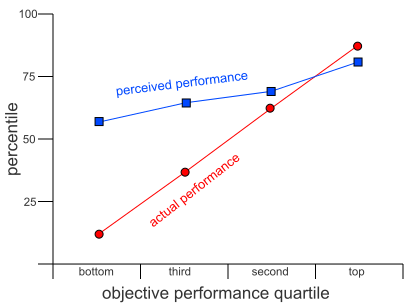
\includegraphics[width=0.95\linewidth]{images/Libro-img001.png}
  \begin{minipage}{\linewidth}
    \caption{By Phlsph7 - Own work, CC BY-SA 4.0, \raggedright\url{https://commons.wikimedia.org/w/index.php?curid=124703870}}
  \end{minipage}
\end{wrapfigure}

L'effetto Dunning-Kruger studiato dagli psicologi David Dunning e Justin
Kruger\endnote{\raggedright\url{https://it.wikipedia.org/wiki/Effetto\_Dunning-Kruger}} è una distorsione cognitiva, dove tendiamo a
sopravvalutare le nostre conoscenze. Sebbene il grafico comunemente associato al fenomeno non provenga dallo studio originale, illustra efficacemente questa percezione distorta iniziale: quando ci cimentiamo in una nuova materia la percezione delle nostre conoscenze (linea blu) è molto più alta delle nostre effettive competenze (linea rossa). Sappiamo quanto sappiamo ma non avendo un quadro completo non sappiamo quanto ancora
c'è da sapere per auto valutare la percentuale del totale della nostra comprensione.

Bertrand Russell "Il problema dell'umanità è che gli stupidi sono strasicuri,
mentre gli intelligenti sono pieni di dubbi"

Più ci si addentra nello studio e nella conoscenza, più ci si rende conto delle innumerevoli ramificazioni del sapere. La
conoscenza diviene pertanto un processo in divenire e mai del tutto esaurito. 

Il nostro cervello per poter fare qualcosa per la prima volta lo simula preventivamente nella mente tramite
l'immaginazione. Vi sarà capitato anche a voi di vedere, un equilibrista, un tuffatore, un
musicista, un influencer e dire, non sembra difficile! Questo perché nella vostra simulazione mentale siete riusciti a farlo senza intoppi! Questa illusione iniziale potrebbe, in certi casi, avere un effetto motivante. Tuttavia, può anche portare a sottovalutare le difficoltà reali e compromettere l’apprendimento o la performance. Ma è anche
un'arma a doppio taglio siccome ci può dare l'illusione di aver acquisito una
certa competenza.

Un fenomeno psicologico spesso considerato speculare è la sindrome dell'impostore, che porta
l'individuo a credere di non meritare i propri traguardi perché crede invece essere dovuti dal
caso, dalla fortuna o dalla sopravvalutazione degli altri. Paradossalmente però, se fossi un vero impostore, difficilmente sperimenteresti la sindrome dell'impostore in quanto non metteresti in dubbio le tue capacità. Non stai cercando di
truffare qualcuno, ma provando solo a fare un buon lavoro. Il fatto di interrogarsi sulle proprie capacità è positivo,
ci porta a migliorare e non finire vittima dell'effetto Dunning-Kruger.

\noindent \textbf{\large Fattore culturale} \\
Nell'Africa sub-Sahariana, in lingua bantu esiste la parola ubuntu. Appellandosi a questa parola si è soliti dire Umuntu
ngumuntu ngabantu, "io sono ciò che sono in virtù di ciò che tutti siamo". L'ubuntu esorta
a sostenersi e aiutarsi reciprocamente, a prendere coscienza non solo dei propri diritti, ma anche dei propri doveri,
poiché è una spinta ideale verso l'umanità intera, un desiderio di
pace\endnote{\raggedright\url{https://it.wikipedia.org/wiki/Ubuntu\_(filosofia)}}. La cooperazione tra umani si è evoluta anche perché, a differenza di molti predatori, la nostra sopravvivenza ha beneficiato notevolmente dalla condivisione di risorse e dall’organizzazione sociale. 
Quindi gli individui che sapevano collaborare e amalgamarsi meglio alle regole
del gruppo venivano premiati dalle risorse condivise, mentre al contrario, chi non aderiva alle norme sociali veniva
ostracizzato e allontanato dal gruppo, condizione che in contesti ancestrali, spesso aumentava drasticamente il rischio per la sopravvivenza dell'individuo.

Anche tra gli esseri umani, alcune ostilità e divisioni possono perpetuarsi nel tempo per via della trasmissione culturale, anche quando si è perso il contesto o la motivazione originaria. In Giamaica nel periodo di lotta per
l'indipendenza dall'Inghilterra si sono formati due partiti in lotta violenta
e armata fra loro: il People's National Party (PNP) e il Jamaica Labour Party (JLP). Nonostante la Giamaica oggi sia
indipendente, la capitale, Kingston, è una delle città più violente al mondo per tasso di omicidi.
Tutt'ora persistono delle zone dove l'accesso è fortemente limitato per chi proviene da territori considerati 'nemici'. Questa divisione, spesso radicata in conflitti passati, si è sedimentata nel tempo, al punto che per molti le ragioni storiche precise possono essere diventate meno chiare, lasciando spazio a una perpetuazione basata sulla tradizione e sull'identità di gruppo.

Secondo una ricerca pubblicata su JNeurosci\endnote{\raggedright\url{https://www.jneurosci.org/content/early/2025/08/18/JNEUROSCI.1018-25.2025}}, l'aggressività può essere contagiosa, principalmente se la si osserva in amici e familiari. Lo studio, condotto su topi maschi, ha osservato che i roditori che assistevano a un attacco da parte di un familiare diventavano a loro volta aggressivi, a differenza di quelli che osservavano l'aggressività in esemplari sconosciuti.

Questo è un ulteriore tassello per comprendere quanto sia importante la consapevolezza. Se facciamo qualcosa e ignoriamo
il momento in cui abbiamo deciso di fare questa scelta e il processo cognitivo che l'ha preceduta, probabilmente è un comportamento appreso da modelli esterni e meno influenzato dal nostro pensiero. Questo può succedere a
tutti, ma è importante ripensare a ciò che facciamo o se possibile accorgerci mentre ci capita e interrogarci,
chiedendoci se questa azione è in linea con i nostri valori, altrimenti potremmo trovarci a seguire direzioni non del tutto allineate con i nostri valori, con il rischio di agire in maniera inautentica.

Per dare alla vita la direzione che vogliamo ed essere più autentici, è talvolta necessario accettare la possibilità di deludere le aspettative altrui.
Dovremmo chiederci: sto agendo in modo coerente con ciò che ho scoperto essere? Con ciò che onestamente credo essere giusto? Non ho danneggiato gli altri? Se le risposte a queste domande sono affermative, allora la critica degli altri, pur restando da considerare, potrebbe assumere un peso differente nella nostra valutazione personale. Tutto questo discorso non vuole sminuire ciò che gli altri mi possono dire, anche questo è importante, ma non rappresenta necessariamente la verità.
L'opinione altrui andrebbe valutata in modo differito, quindi non reagendo a caldo ma prendendoci del tempo, anche giorni, per pensarci su. Tante volte le cose che ci vengono dette, dicono più degli altri che di noi stessi.
Abbiamo detto del come, del quando, ma di chi dare peso alle opinioni? Da chi si è guadagnato la nostra stima.
Noi siamo il risultato delle nostre azioni, delle nostre scelte, quelle giuste e quelle che abbiamo riconosciuto come sbagliate. Non dovremmo sentirci costretti a cambiare per conformarci alle aspettative altrui. Gli altri possono scegliere se stare con noi o no. Questa è la persona che sono oggi, e penso sia giusto fare le mie scelte, e tracciare, con anche gli errori, la mia via.
Prendere in considerazione il parere altrui è positivo, ma poi seguirlo non è un obbligo. 

\begin{mdframed}[linewidth=1pt]
Stigma del fallimento

Noi europei, in particolare gli italiani, spesso viviamo il fallimento con vergogna. Dobbiamo essere sempre
perfetti, informati, produttivi, risolutivi, ma questo è impossibile in un mondo complesso dove
l'asticella continua ad alzarsi. Cosa ci sarebbe di male se non sapessimo fare qualcosa? o se non
conosciamo qualcosa? o se abbiamo bisogno di aiuto? Non solo, è molto difficile fare qualcosa di nuovo senza fallire. Se non fallisci forse non ti stai ponendo obiettivi ambiziosi (e andrebbe bene anche così).

Thomas Edison raccontò che fece numerosi tentativi prima di riuscire ad accendere la prima lampadina. Henry Ford affrontò due crac, poi fondò la Ford Motor Company. Gli esempi potrebbero continuare ad oltranza.

Non avrai mai fallito finché continuerai a provare (Anonimo).

In alcuni contesti imprenditoriali statunitensi, come la Silicon Valley, il fallimento è considerato parte integrante del percorso verso il successo. Nel mondo startup si è diffusa l’idea del ‘fail fast, learn faster’, ovvero sbagliare presto per imparare rapidamente dai propri errori. Ogni
fallimento può essere analizzato e, una volta individuati i problemi, farne tesoro per aggiustare il tiro e, fare
meglio la volta successiva. 

Viviamo la vergogna del fallimento come qualcosa di sociale. Quando sperimentiamo cose nuove infatti, cerchiamo di farlo da soli. Se sbagliamo e, siamo da soli, non è un
problema, perché nessuno si è accorto, è come se non fosse mai successo. Lo stesso identico errore davanti ad altri
invece può essere vissuto con vergogna. La paura costante di fallire può spingere alcune persone a cercare ambienti in cui le proprie idee siano sempre confermate, riducendo l’apertura mentale e la crescita intellettuale. Da piccoli quando inciampavamo,
non stavamo a rimuginare su cosa pensavano gli altri, su come fosse potuto accadere, su cosa avremmo potuto fare,
semplicemente ci rialzavamo e continuavamo, senza giudicarci. In questo modo il male della caduta scorreva via più velocemente e veniva trattenuto meno dai nostri pensieri. 

“Io non perdo mai: o vinco o imparo.” - Nelson Mandela 
\end{mdframed}

\noindent \textbf{\large De-responsabilizzazione} \\
Verso la metà del 900, lo psicologo J. B. Rotter parlò di “Locus of control” (“luogo di controllo”) ovvero, la
percezione di quanto la propria vita sia influenzata dalle proprie azioni o dalla casualità e, di conseguenza, a quali
di questi due fattori si attribuiscono successi e insuccessi. In alcuni casi, le persone tendono ad attribuire i propri successi a fattori interni e i fallimenti a cause esterne, un meccanismo noto come attribuzione auto-protettiva. 
Apparentemente ci stiamo proteggendo la nostra autostima in questo
modo, in realtà ci stiamo privando di avere la percezione di poter agire e intervenire sul mondo. Ovviamente non
possiamo pensare che tutto sia sotto il nostro controllo, se lo credessimo potremmo cadere in altre problematiche, come
detto in precedenza dovremmo pian piano imparare ad accettare l'incertezza. Coltivare un senso di autoefficacia, ovvero la convinzione di poter influire su ciò che ci accade, può aiutarci ad affrontare meglio le difficoltà, purché resti ancorato alla realtà e non si trasformi in un’illusione di controllo totale. Se qualcuno ci tratta male, anche se lui rimane il maleducato, ma
ci chiediamo: come posso pormi prossima volta per evitare questa reazione? O ancora, posso aver agevolato in qualche
modo questa reazione? Questo atteggiamento ci dona una possibilità di cambiamento. Se invece pensiamo che lui ha
sbagliato e basta, cosa che potrebbe anche essere vera, rischiamo di essere in balia degli eventi e meno efficaci a gestire le situazioni che ci accadono.

Una cosa su cui sono piuttosto sensibile è proprio questo tipo di narrazione, sembra che si cerchi un colpevole più che una soluzione. Che si tratti del partner, dell'insegnante, della dirimpettaia,
del governo o delle scie chimiche. Di esempi ce ne sono tanti, un collega o un superiore che incolpa la mancata
consegna di un lavoro mal schedulato da lui. Una mamma che incolpa gli insegnanti per i pessimi voti del figlio,
l'insegnante per il disimpegno degli studenti, gli studenti dicendo che la loro scuola fa schifo,
non argomentando con un generico: “non c'è organizzazione”, manca il lavoro e così via
all'infinito.

È frequente sentire lamentele 'è colpa del governo', in un contesto in cui si verificano comportamenti come l'evasione fiscale, pratiche scorrette sul lavoro (es. timbrare il cartellino per un collega assente), abusi dei permessi di malattia, indebite richieste di invalidità, infrazioni stradali. Alcuni cittadini criticano aspramente la società ma contribuiscono anche al mantenimento di certi problemi.
L’evasione fiscale riduce le risorse disponibili per i servizi pubblici, contribuendo a una percezione di inefficienza del sistema. In questo senso, la responsabilità collettiva gioca un ruolo cruciale.

\noindent \textbf{\large Suggestioni} \\
Effetto Priming\endnote{\raggedright\url{https://it.wikipedia.org/wiki/Priming\_(psicologia)} }: Questo effetto dice che
l'esposizione a uno stimolo può influenzare la tua risposta.
Ad esempio, dopo aver letto la parola ospedale, una persona riconoscerà più rapidamente parole come medico o iniezione. Oppure, vedere immagini legate alla pulizia può indurre le persone a comportarsi in modo più ordinato.

Quanto detto è contrario alla filosofia: fake it until you make it, ovvero, fingi fino a quando non lo ottieni, figlia
di alcuni movimenti motivazionali, che grazie a frasi auto-motivazionali promettono di farti raggiungere certi risultati
personali e farti diventare una persona diversa. Queste tecniche si
utilizzano quando un atleta deve affrontare una gara, in questo caso possono funzionare perché applicate su un soggetto che prima di tutto ha passato tempo ad allenarsi e ad acquisire le competenze per affrontare quel determinato compito. Queste tecniche però possono essere pericolose, perché, se
immaginiamo tante volte noi che riusciamo a superare una difficoltà, quando si presenterà davvero, potremmo abbassare la
guardia e l'impegno perché convinti di saper gestire quella determinata situazione. Essere in uno
stato mentale negativo e credere di non farcela potrebbe portarti a non farcela, ma al contrario, se noi siamo sicuri di
farcela questo non sarà sufficiente a garantirci il successo. Quindi va bene prefigurarsi un nostro stato mentale o le
varie ipotesi, ma tenendo presente che le nostre aspettative potrebbero non realizzarsi. Questo effetto però
agisce solo fino ad un certo punto, probabilmente non cambierà la nostra personalità o il nostro umore sul lungo periodo. Se sei
un atleta e ti influenzi affinché tu ti senta più forte e concentrato, la tua performance sarà migliore, ma è solo la
ciliegina sulla torta, alla base deve esserci un duro allenamento. Non basta ripetersi di essere milionari o felici
per diventarlo. Allo stesso modo vale anche al contrario, se mi dico che sono un imbranato, non è detto che lo diventerò.
L'efficacia di suggestioni e frasi motivazionali possono essere limitate, in quanto consapevole sai che ti stai suggestionando. Le suggestioni funzionano meglio quando sono nascoste e non ne siamo consapevoli, come succede ad esempio in certe pubblicità. 

Un altro effetto interessante che ci condiziona inconsapevolmente è l'effetto placebo e anche il
suo opposto meno noto effetto nocebo. L'effetto nocebo è un condizionamento in negativo, se
diciamo a una persona che questo macchinario potrebbe provocarti del dolore, probabilmente lo farà, anche se si tratta
di una lampada che fa un leggero calore\endnote{\raggedright\url{https://youtu.be/OUdXMoY6fLY}}.

\noindent \textbf{\large Altre distorsioni comuni} \\
Errori di ragionamento chiamate fallacie induttive, ovvero, pensare che se è successo una volta allora succederà sempre.
Se una cosa è vera una volta allora lo sarà sempre. Vediamo alcuni esempi:

\begin{itemize}
\item Generalizzazione indebita: Un uomo ha rubato una mela. Quindi tutti gli uomini sono ladri.
\item Generalizzazione statistica: "tre studenti di matematica sono introversi" e concludere che "tutti gli studenti di matematica sono introversi". Il campione è troppo piccolo.
\item Fallacia del giocatore: Se gioco alla roulette ed è uscito il rosso per cinque volte, molto probabilmente ora
uscirà il nero. Statisticamente invece ogni volta, rosso e nero hanno la stessa probabilità di uscire.
\item Falsa causa: Ho rotto uno specchio e ora va tutto storto. La scaramanzia, ma non solo, rientra in questa
tipologia, quando si cerca di spiegare qualcosa con una causa la quale non è strettamente legata con
l'effetto
\item Fallacia dell'evidenza soppressa: Nelle prossime pagine vedremo alcuni esempi. In sostanza si tratta di omettere
delle informazioni importanti e che quindi daranno una visione della questione anche diametralmente opposta.
\end{itemize}

Si parla di fallacie di presupposizione quando le premesse sono anche le conclusioni della nostra tesi, per indurre
l'interlocutore alla stessa soluzione.

\begin{itemize}
\item Fallacia patetica: Credere che tutto si comporti con una logica umana. Ad esempio agli umani piace essere liberi,
quindi anche l'aria e, per questo esiste la pressione in fisica. O la paura che i robot e
l'intelligenza artificiale un giorno si ribelleranno e conquisteranno il mondo. La conquista del
mondo o la prevaricazione su altre specie, in senso antropocentrico, non sono dinamiche così frequenti in natura, è un ambizione principalmente umana, e non c'è motivo di credere che un robot umanoide abbia i medesimi desideri.
\item Circolarità semplice: Tra le premesse di un'argomentazione figura la tesi che si vuole sostenere. Per esempio: Dio
ha creato il mondo, dunque Dio esiste. Dio esiste, dunque è stato Dio a creare il mondo.
\item Domanda multipla: quando nella domanda si dà per scontato qualcosa che non è stato ancora dimostrato. Esempio: Mi
spieghi come hai fatto a copiare il compito in classe?
\item Fallacia della conclusione sbagliata: Ad esempio dimostriamo che l'inflazione sta scendendo e
ne concludiamo che l'economia sta andando bene. Le premesse però non sostengono la conclusione.
\item Falsa pista: Esempio: Il Paese è sotto la minaccia del terrorismo. Urge acquistare nuovi armamenti sempre più
potenti. Il terrorismo non si combatte necessariamente con l'acquisto di nuovi armamenti. Possono essere efficaci anche
quelli già in dotazione, si può aprire una trattativa, un dialogo ecc…
\item Argomento fantoccio: confutare una tesi apparentemente simile a quella che si vuole negare o confermare così, per
conseguenza logica, cade o viene confermata anche la tesi principale. Esempio: Darwin ha commesso questi errori, quindi
tutta la teoria dell'evoluzione è falsa.
\end{itemize}

Fallacie formali e informali

\begin{itemize}
\item Argomentazione a catena: Si giunge a una conclusione erronea tramite un processo di reazione a catena, come ad
esempio, chi prova le droghe leggere come la cannabis, arriverà a provare anche la cocaina, perché cercherà sempre
qualcosa di più forte.
\item Tu quoque: X sostiene che si dovrebbero pagare le tasse, ma siccome X è un evasore fiscale, le tasse non vanno
pagate.
\item Accusa d'interesse: Se c'è un conflitto d'interesse allora
l'oggetto in discussione è necessariamente falso.
\item Colpa per associazione: X sostiene una testi, ma X è anche amico di spacciatori. Quindi X non è una persona
rispettabile e la sua tesi di conseguenza.
\item Appello all'autorità: Prendere per vera o falsa una tesi perché “l'ha detto X”. Il classico
ipse dixit o “l'ha detto la televisione”.
\item Appello alla modestia: Al contrario dell'appello all'autorità, si è portati a credere a una teoria minore, di
nicchia e, non ancora riconosciuta.
\item Ad judicium: Se lo dicono tutti allora sarà vero. Da qua nascono alcune credenze popolari come: scrocchiare le dita fa venire l'artrite, il freddo fa ammalare, se cade qualcosa per terra per meno di cinque secondi si può mangiare, il cioccolato
fa venire i brufoli, lo zucchero di canna è più salutare di quello bianco. Le affermazioni appena citate sono tutte
false\endnote{\raggedright\url{https://www.focus.it/scienza/salute/bugie-salute}.}
\item Argumentum ad ignorantiam: Si giustifica la propria tesi con la mancanza di prove del suo contrario.
\item Fallacia della brutta china: Fa appello alle conseguenze negative della tesi da rigettare.
\end{itemize}

Altre distorsioni:

\begin{itemize}
\item Bias di conferma: credere a informazioni che confermano ciò che già sappiamo.
\item Effetto incorniciamento: presentare una teoria mostrando solo aspetti negativi o positivi influenza il giudizio.
Anche il contesto è importante, uno sconto a tempo ci farà essere più frettolosi nell'acquisto 
\item Bias del costo sommerso: Portare avanti un lavoro, un progetto, o una relazione solo perché interrompendola si
perderebbero tutti gli investimenti di tempo soldi e energie passate
\item Euristica dell'affetto: valutare un’azione come buona o giusta basandosi sulle emozioni o sentimenti associati, senza analisi analitica delle evidenze
\item Euristica della disponibilità: Ad esempio quando il telegiornale parla spesso di una cosa, che magari è un evento
raro ma ci inizia a sembrare invece molto frequente 
\item Astrazione selettiva: si presta attenzione ad un solo aspetto o a un solo dettaglio della situazione. Gli aspetti
positivi sono spesso ignorati a vantaggio di quelli negativi o viceversa.
\item Pensiero dicotomico: gli eventi sono valutati in forma estrema, del tipo buono / cattivo, nero / bianco, on / off,
etc.
\item Inferenza arbitraria: vengono tratte conclusioni da situazioni non supportate dai fatti, anche quando
l'evidenza è in contrasto con la conclusione.
\item Supergeneralizzazione: si giunge a una conclusione generale partendo da un evento particolare.
\item Ingigantire e minimizzare: si assume la tendenza a esagerare gli aspetti negativi di una situazione, riducendo al
minimo il positivo.
\item Personalizzazione: interpretare erroneamente eventi esterni come causati da se stessi o riferiti a sé, senza evidenze oggettive.
\item Visione catastrofica: si anticipano gli eventi pensando che il peggio accadrà sicuramente.
\item Doverizzazione: ci si auto-impone regole rigide e severe su come le cose dovrebbero andare.
\item Variabili globali: vengono utilizzate etichette generali sugli eventi che non considerano le diverse sfumature.
\item Bias di ancoraggio: propensione a prendere decisioni basandosi sulle prime informazioni trovate, utilizzate come
riferimento per i ragionamenti successivi. Per esempio, il primo prezzo offerto per un'automobile di seconda mano
imposta lo standard per il resto della negoziazione. Un prezzo inferiore sembrerà ragionevole anche se superiore al
vero valore dell'automobile.
\item Apofenia: nota anche come patternicity, o agenticity, è la tendenza umana a trovare spiegazioni, soluzioni,
schermi ricorrenti tra dati casuali e senza una vera spiegazione statistica.
\item Hindsight bias: o bias del senno di poi è la tendenza delle persone a credere, erroneamente, di aver saputo
prevedere un evento correttamente, una volta che l'evento è ormai noto. 
\item Outcome bias: o bias del risultato è la tendenza a rileggere il passato con gli occhi e
l'esperienza di oggi modificando la storia attorno a quell'evento.
\item Bias dei dettagli seduttivi: valutare un argomento credibile solo perché includa dettagli veri, ma irrilevanti per la logica o la robustezza dell’argomentazione\endnote{\raggedright\url{https://www.stateofmind.it/2018/07/distorsioni-cognitive/}}
\endnote{\raggedright\url{https://it.wikipedia.org/wiki/Bias\_cognitivo}}. 
\end{itemize}

Queste sono solo alcune delle fallacie studiate. Abbiamo anche quelle che fanno appello alle emozioni, che portano a
cambiare opinione per paura o compassione, usate molto in televisione\endnote{\raggedright\url{https://it.wikipedia.org/wiki/Fallacia}}.

\noindent \textbf{\large Libero Arbitrio} \\
Prendiamo decisioni attraverso schemi mentali o automatismi fallaci, bias cognitivi, di cui non ci rendiamo conto. I
bias cognitivi che abbiamo visto precedentemente sono comuni, con percentuali più o meno diverse. In più,
ognuno di noi sviluppa degli schemi mentali suoi, che sono unici, ma di cui non sempre ne è a conoscenza, ma da cui può
dipendere la propria vita e le proprie decisioni. Proprio ora, mentre stai leggendo, sei consapevole della tua
posizione? Come sono posizionati i tuoi arti? Qualcuno di voi avrà le gambe accavallate, incrociate, o con una mano che
sorregge la testa ecc… Ora che l'hai letto, sei consapevole della posizione che ha assunto il tuo
corpo, ma fino a un attimo fa no. Eppure è stato il tuo cervello a metterti in quella posizione e, continuava a mandare
impulsi affinché tu mantenessi quella posa. Hai scelto di metterti in quella posa? O l'ha scelto
il tuo cervello? E come mai ha scelto proprio quella e non un'altra? A volte capita che guidando
l'auto per andare al supermercato, siamo sovrappensiero e ci ritroviamo a casa. Oltre a gestire i nostri sistemi, che ci consentono di sopravvivere, come far battere il cuore, respirare ecc… il nostro cervello
è in ascolto dei nostri cinque sensi. Se ci arriva qualcosa in faccia all'improvviso,
chiudiamo gli occhi, giriamo la testa e ci proteggiamo con le mani, senza nemmeno pensarci. Se in una stanza rumorosa
stiamo leggendo, riusciamo a isolarci da tutte le parole e, riusciamo a non seguire i discorsi degli altri, ma se
qualcuno ci chiama, noi ci accorgiamo. Questo vuol dire che in realtà il nostro cervello ha analizzato i vari suoni,
li ha convertiti in parole, li ha analizzati e valutato che tutte le parole non dovevano essere mostrate
alla consapevolezza, alla nostra attenzione, tranne una, che invece poteva interessargli. Questi automatismi, questi
nostri schemi mentali, riguardano solo queste azioni automatiche? In realtà no, come vedremo nel capitolo sui
dibattiti, molte delle nostre decisioni, soprattutto quelle più rapide o complesse, sono fortemente influenzate da fattori emotivi. Tendiamo a valutare ciò che è 'giusto' o 'sbagliato' anche in base alle nostre reazioni istintive e preferenze, e solo in un secondo momento possiamo costruire una giustificazione razionale della nostra scelta, talvolta convincendoci della sua logicità.
Anche quando cerchiamo di prendere una decisione con il ragionamento, mettendoci in discussione, con il massimo
dell'onestà intellettuale, il nostro dialogo interiore, sebbene possa esplorare diverse prospettive, seguirà inevitabilmente un percorso influenzato, se non plasmato, dai nostri schemi mentali preesistenti.

In modo simile a quanto osservato nell'esempio della postura, alcuni studi suggeriscono che, in certi contesti, il cervello possa avviare un'azione prima che se ne divenga pienamente consapevoli. In questi casi, la sensazione di aver preso una decisione cosciente potrebbe emergere solo dopo che il processo è già iniziato a livello neurale. Questo fenomeno, sebbene oggetto di intenso dibattito, ha portato alcuni a postulare che il libero arbitrio, almeno per certi tipi di decisioni, possa essere in parte un'illusione o un'interpretazione a posteriori. Il nostro cervello ha sviluppato quindi questa strategia per
essere più efficiente, prendere decisioni immediate, come i riflessi, senza sottoporle alla coscienza, che è più lenta
nell'elaborazione. Il cervello, per essere veloce, non mette in discussione ogni singola
questione, anzi, non lo fa nella maggioranza dei casi. Il cervello approssima, etichettando, dando un nome a un determinato fenomeno e,
attuando simili soluzioni, che ha visto funzionare in passato, per un evento che reputa dello stesso tipo.
Questa strategia è efficiente in termini di velocità decisionale ma meno nell'accuratezza. Questo pregiudizio, ovvero, giudicato prima, prima di un'attenta, ma lenta analisi, tende a semplificare e trovare pattern anche dove non ci sono (apofenia), il che può favorire la formazione di superstizioni, credenze pseudoscientifiche o credenza in teorie del complotto. La vita
moderna ci sottopone continuamente a una moltitudine di informazioni, di sollecitazioni e il nostro cervello fatica ad elaborare tutto. Così, gli stessi schemi mentali o automatismi, necessari e che funzionano bene per la maggioranza di casi, possono essere applicati anche in altri contesti, inclusi quelli che coinvolgono decisioni etiche e morali, non sempre con gli stessi risultati ottimali. 
Ad esempio, quando controlliamo compulsivamente le notifiche sul telefono, spesso potrebbe non essere una scelta consapevole. Arriva una notifica e in automatico, meccanicamente, tanti di noi guardano il telefono, senza che ci sia un pensiero che ci chieda quanto sia utile in questo momento, questo comportamento. Questi risultati suggeriscono che il libero arbitrio potrebbe essere limitato in compiti semplici automatizzati, ma la sua estensione nella vita reale, più complessa, richiede ulteriori ricerche. Anche se riuscissimo a liberarci dalla dipendenza dal telefono, continueremmo comunque a ricevere incessanti stimoli esterni che possono influenzare le nostre azioni influenzate dai nostri schemi mentali.

Ma come si formano gli schemi mentali? Il nostro cervello e formato da neuroni che sono collegati tra loro da sinapsi. Se dobbiamo
raggiungere un luogo che non conosciamo, per esempio un nuovo posto di lavoro, la prima volta chiederemo informazioni,
guarderemo i cartelli, alla fine riusciremo ad arrivare fino alla nostra destinazione, magari un po' a tentativi anche
e, facendo strade sbagliate. Questa nostra esperienza avrà creato delle nuove connessioni neuronali, delle sinapsi. Ora
abbiamo diversi nuovi collegamenti, anche se deboli. Il giorno dopo ci troveremo a raggiungere nuovamente il posto di
lavoro, abbiamo capito la zona e fino a li ci arriviamo senza problemi, magari sbagliamo ancora un paio di svolte, ma è
comunque andata meglio del giorno prima. Con questa nuova esperienza, inizieremo a rafforzare alcune connessioni
neuronali e abbandonarne altre. I primi giorni impareremo a raggiungere il luogo di lavoro, in più, sperimenteremo
nuove strade, per metterci meno tempo, evitare il traffico ecc… Una volta che troviamo la strada secondo noi migliore,
tutti i giorni percorreremo sempre la stessa strada e quelle connessioni neuronali, che ci permettono di raggiungere il
posto di lavoro, facendo quel preciso percorso, diventano sempre più forti, creando uno scherma mentale forte. Quando
si hanno connessioni forti in un certo contesto si può generalmente sperimentare un'elasticità mentale minore. Per questo può essere utile fare alcuni esercizi come,
cambiare strada per tornare a casa o sedersi a tavola in posti diversi da quelli usuali.

Negli anni alcuni scienziati hanno cercato delle prove circa l'illusione del libero arbitrio.
Benjamin Libet chiese a dei volontari di premere un pulsante che si trovava davanti a loro e, potevano farlo in
qualsiasi momento, quando lo preferivano. I partecipanti all'esperimento sono stati monitorati con
un elettroencefalogramma. Il risultato fu che l'attività cerebrale nota come 'potenziale di prontezza' (Bereitschaftspotential) emerge circa 550ms prima dell’azione, mentre la consapevolezza della volontà nasce circa 200ms prima del movimento.
Forse può sembrare un tempo irrisorio, ma per il sistema nervoso, dove le informazioni viaggiano a centinaia di metri
al secondo è un tempo importante. Nel 2008, uno studio\endnote{C. S. Soon,
"Unconscious determinants of free decisions in the human brain", Nature
Neuroscience} con fMRI ha identificato attività corticali (in corteccia prefrontale e parietale) che permettevano di predire la scelta (pulsante destro o sinistro) fino a 10 secondi prima della consapevolezza della decisione.
 
A seguito di questi esperimenti, psicologi come Daniel Wegner hanno sviluppato teorie secondo cui la percezione della nostra volontà cosciente di agire potrebbe, in alcuni contesti, essere un'esperienza che segue, piuttosto che precedere, l'avvio inconscio dell'azione da parte del cervello.
Il cervello integra stimoli ambientali e predisposizioni biologiche/genetiche (che non possiamo scegliere) nella formazione degli schemi mentali che influenzano le decisioni. Secondo alcune interpretazioni (es. Wegner), il senso di volontà è posteriore alla decisione inconscia; tuttavia Libet stesso ha evidenziato il ruolo del 'veto cosciente' che può inibire un'azione già avviata.

Se hai avuto la fortuna, la casualità, di vivere in un ambiente che ti ha fornito condizionamenti positivi, che ha
permesso lo sviluppo di certe connessioni neuronali, sarai più avvantaggiato rispetto a una persona che, sempre
casualmente, è cresciuta in un ambiente che gli ha fornito uno schema mentale potenzialmente meno adattivo o che può generare maggiore sofferenza. A questo va aggiunto una componente genetica anch'essa ereditata dal caso, su cui non
abbiamo potuto avere controllo. E come vedremo successivamente non accettare questi schemi, ignorarli, fare finta che
non esistano, può portare a problemi.

Anche questo esperimento va visto nella giusta prospettiva, nella sua “via di Mezzo”. Premere un pulsante è un
operazione semplice, molto soggetta ad automatismi e, grazie ai neuroni specchio che permettono al cervello di attivare aree cerebrali simili sia durante l'esecuzione di una determinata azione sia nel momento dell'osservazione o del pensiero di essa, facilitando l'apprendimento e l'empatia. Potete trovare questo esperimento e
molti altri all'interno della serie Mind
Field\endnote{\raggedright\url{https://www.youtube.com/watch?v=lmI7NnMqwLQ}}.

Un altro esperimento interessante è stato svolto in America nel periodo John Kerry e George W. Bush. Sono stati presi
due gruppi di cittadini, democratici e repubblicani, a cui sono stati mostrati dei video, dove i due politici cadevano
in evidenti contraddizioni. I democratici percepivano le contraddizioni del presidente repubblicano. Ma non percepivano
le contraddizioni del politico democratico. E viceversa succedeva per i repubblicani. Non solo perché le persone
sottoposte all'esperimento esprimevano verbalmente questa sensazione, ma anche a livello celebrale
che è stato monitorato grazie all'uso dell'elettroencefalogramma.

Altro esperimento interessante, svolto in un'università americana: Sono state prese delle
matricole, ragazzi appena iscritti, che ancora non conoscevano i professori che avrebbero avuto durante
l'anno. I ricercatori hanno mostrato ai ragazzi brevi video di trenta secondi circa, dei
professori che avrebbero avuto durante l'anno e, in base a questi, di fare una classifica dei
docenti migliori, in base a questa prima impressione. A fine anno, i ragazzi hanno avuto modo di conoscere davvero i
professori visti in quei video, ed è stato chiesto loro di rifare nuovamente la classifica dei professori più bravi.
Questa volta con cognizione di causa. Il risultato fu che la classifica è rimasta sostanzialmente invariata. Anche in
questo caso, la prima impressione, il pregiudizio inconscio ha avuto un influenza sulla mente conscia e la parola. Prima arriva
la sensazione e poi la consapevolezza e la parola\endnote{\raggedright\url{https://www.youtube.com/watch?v=NHB-qw9XlXI}}.
Generalizzando, noi agiamo e successivamente giustifichiamo il nostro agire, come se l'avessimo
scelto noi. Questo fenomeno è stato osservato anche in un esperimento che coinvolgeva un bar dove principalmente si
vendevano bibite gassate. Cambiando la disposizione dei prodotti e dell'arredamento in modo da
favorire il consumo di acqua, si notò che le vendite aumentarono. Così, è stato chiesto alle persone come mai avessero
scelto di comprare l'acqua che risposero: perché ne avevamo voglia. Ipotizziamo che questo sia improbabile, in quanto, prima del cambio di arredamento si preferiva comprare bibite gassate. Questo ci
suggerisce che noi agiamo grazie ad una concomitanza di fattori tra cui quelli ambientali e poi, successivamente,
giustifichiamo questa nostra scelta. Questo effetto può essere usato anche a nostro favore,
infatti, se vogliamo cambiare una nostra abitudine possiamo intervenire sull'ambiente che ci
circonda, in modo da agevolare un certo comportamento.
Ricordiamoci che se ad esempio mettiamo dei post-it che ci ricordino di fare qualcosa, ogni due o tre giorni possiamo cambiargli di posto o cambiare frasi, altrimenti ci abitueremo alla loro vista iniziando ad ignorarli.
per introdurre un abitudine dovrebbe essere a meno di 20 secondi da dove ti trovi
in quel momento
Un ostacolo importante quando si tratta di ottenere un cambiamento nella propria vita, anche se un po' controintuitivo, sono le dipendenze, come suggerisce il dottor Valerio Rosso che conduce un podcast dove affronta questi argomenti. Quando si parla di dipendenze pensiamo alle droghe, all'alcohol, al gioco d'azzardo, ma in realtà sono molte di più, come la dipendenza da smartphone, televisione o più in generale dall'intrattenimento costante, ma anche dagli zuccheri, dal non poter sbagliare, dipendenze affettive e tutto ciò verso cui compulsivamente tendiamo e a cui facciamo fatica a rinunciare. Quindi se non riesci a cambiare stile di vita potrebbe essere pigrizia, mancanza delle giuste informazioni, bassa energia, ma forse no o non solo. Quindi il primo passo è capire quali sono queste dipendenze, che cosa ci sta controllando, dove va la nostra mente quando stiamo cercando di cambiare stile di vita e, non pensate solo alle dipendenze "classiche".

Un giorno, Freud si trovava alla festa di Capodanno organizzata da Jean-Martin Charcot, uno dei suoi mentori a Parigi
durante i suoi studi sull'ipnosi. Charcot, per dimostrare la sua abilità ipnotica, ipnotizza un uomo e gli ordina di
aprire l'ombrello al centro della sala quando scocca la mezzanotte. Freud, incuriosito, segue l'uomo e gli chiede il
motivo dell'apertura dell'ombrello. L'uomo risponde che lo sta facendo perché piove, ma Freud gli fa notare che sono al
chiuso. L'uomo, incapace di rispondere adeguatamente, continua a cercare una spiegazione, dicendo che ne aveva voglia,
senza rendersi conto di essere stato ipnotizzato e di seguire degli ordini. Freud riflette su come questa situazione
possa riflettersi nella vita di tutti i giorni. Si chiede se i suoi problemi derivino dal fatto di essere stato
condizionato dalla cultura familiare e sociale, senza rendersene conto. Capisce che molte volte, quando cerchiamo di
giustificare le nostre azioni, stiamo razionalizzando delle difese psicologiche, piuttosto che
comprendere le nostre motivazioni che stanno alla base. Questo porta Freud a interrogarsi sul ruolo dell'ipnosi nella
formazione dei comportamenti umani e nel processo decisionale.

Quindi dobbiamo arrenderci al destino? Qualsiasi nostro sforzo è inutile perché tutto è già stato scritto?
Fortunatamente no, altrimenti dovremmo aprire tutte le carceri e lasciare a piede libero gli assassini in quanto non
avrebbero colpa. Da una prospettiva più deterministica, alcune interpretazioni potrebbero suggerire che sia effettivamente così. Alcuni studi hanno individuato correlazioni tra tratti antisociali e anomalie in specifiche aree cerebrali (es. amigdala, corteccia prefrontale), suggerendo una componente biologica, ma non esclusivamente genetica o deterministica. 
Alcune persone potrebbero compiere omicidi di massa a
seguito di un tumore al cervello, anch'esso, non deciso e voluto da loro. Alcuni ricercatori,
nelle carceri, dividendo i carcerati per crimine commesso, hanno notato che i vari gruppi presentavano particolari geni
meno frequenti negli altri gruppi. Emblematico il caso del giudice Hannover che ha dato un fortissimo sconto della pena
per lo stupro di una ragazza. La motivazione? Lo stupratore era sardo. "Si deve tenere conto delle
particolari impronte culturali ed etniche dell'imputato. È un sardo. Il quadro del ruolo dell'uomo e della donna,
esistente nella sua patria, non può certo valere come scusante ne deve essere tenuto in considerazione come attenuante".
\endnote{\raggedright\url{https://www.lagazzettadelmezzogiorno.it/news/home/65714/germania-torturo-una-ragazza-sconto-di-pena-e-sardo.html}}

Noi abbiamo la scelta, ma ci comportiamo con schemi seppur complessi, potenzialmente prevedibili, se potessimo leggere
nel cervello. Riprendendo l'esempio della strada per andare al lavoro, i nostri schemi mentali,
diventano automatici dopo un'elaborazione della mente conscia, più
l'influenza della genetica e di altri schemi mentali pregressi, più la casualità degli eventi. Tra questi vari punti abbiamo l'elaborazione della mente conscia su cui possiamo avere un minimo di manovra. Un minimo perché la nostra mente conscia è influenzata dalla mente inconscia, schemi mentali, bias
cognitivi, preconcetti ecc… Quindi non va visto come un destino scritto nelle stelle. È qualcosa di più locale, è la
nostra mente che ci condiziona, che ci da una “tendenza” seppur molto forte a comportarci e pensare in un certo modo.
Uno studio del 2019 (UNSW)\endnote{\raggedright\url{https://www.nature.com/articles/s41598-019-39813-y}}, con risonanza magnetica, ha osservato che modelli di attività cerebrale predittiva delle scelte emergono prima della consapevolezza, suggerendo una predisposizione inconscia, ma l’accuratezza non è mai stata del 100\%.
Questo significa che qualcuno tra i partecipanti ha preso
una decisione a livello inconscio e in quei 200 millisecondi abbia cambiato la
scelta\endnote{\raggedright\url{https://www.focus.it/comportamento/psicologia/scelte-visibili-cervello-prima-volonta}}.

Se diventi consapevole di avere un problema, o che ti stai auto sabotando,
convincendoti di qualcosa solo perché è più comodo, o di non star facendo la cosa giusta, allora puoi intervenire.
Un po' come quando notato che ora stai assumendo una certa posizione. Ora che ne sai consapevole puoi
cambiarla. È anche vero che diventerai consapevole o meno di qualcosa, influenzato dai tuoi schemi mentali,
però parlando con qualcuno, magari in un momento difficile, facendo associazioni libere di pensieri, scrittura
creativa, meditazione ecc... puoi cercare di allentare la presa dei tuoi schemi mentali e,
lasciare che ci sia una fuoriuscita e, che affiori anche alla consapevolezza di alcuni tuoi lati.

La cultura occidentale, teorizzata poi da Freud con il concetto di "io" presuppone che,
tolte tutte le nostre maschere troveremo il nostro vero io. Mentre alcune branche della nuova psicologia non vedono
l'io dietro tutte le maschere, ma l'io come tutte quelle maschere. È difficile trovare un ‘io’ definitivo, perché la vita e, le sue
situazioni, ti potrebbero mostrare un io diverso da ciò che credevi e, successivamente, definito questo tuo nuovo io, potrebbe venire
contraddetto anche quest'ultimo dalle nuove concomitanze. L'io, più che una caratteristica fissa, può essere inteso come un processo in continuo divenire, un'esperienza che si manifesta e si ridefinisce in ogni momento, fortemente legata al contesto e all'interazione con il mondo, in un flusso costante. Il classico panta rei, tutto scorre, non ci si può immergere due volte nello stesso fiume, perché quel fiume
ora si è spostato più a valle.

Questa complessità della nostra rete neurale implica che, anche a fronte di situazioni apparentemente simili, le risposte possano variare leggermente. È fondamentale tenere conto di questa complessità, pur mantenendo un quadro di responsabilità indispensabile per la coesione sociale. In sintesi, sebbene la questione del libero arbitrio resti profondamente dibattuta e alcuni studi ne mettano in discussione l'esistenza nel senso più assoluto, la nostra esperienza e la necessità di una società organizzata ci impongono di agire e di assumerci le responsabilità come se esso fosse pienamente operativo.

\needspace{4cm}
\begin{mdframed}[linewidth=1pt]
Esperimento del piccolo Albert

\begin{wrapfigure}{i}{9cm}
  \centering
  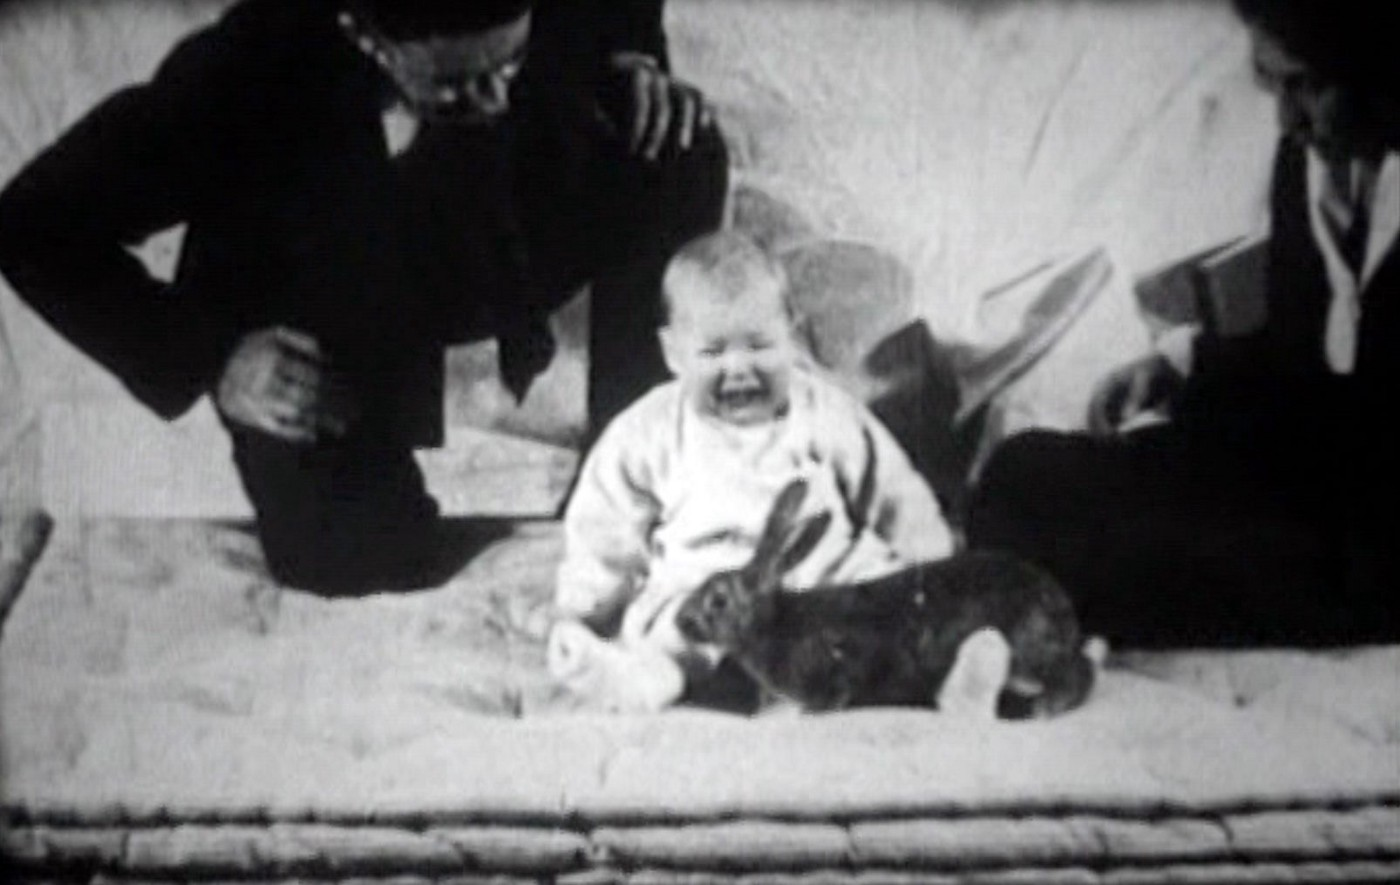
\includegraphics[width=0.95\linewidth]{images/Libro-img002.jpg}
  \begin{minipage}{\linewidth}
    \caption{Un frame estratto dai video girati dal Dr. John Watson e Rosalie Rayner.}
  \end{minipage}
\end{wrapfigure}

Jhon Broadus Watson, nato nel 1878, è conosciuto come il padre del comportamentismo. Voleva dimostrare con un bambino i
cui pattern in risposta agli stimoli sono piuttosto semplici rispetto a un adulto, che si possono indurre, attraverso
il condizionamento ambientale, alcune emozioni come la paura. Albert era un neonato e ha circa 9 mesi quando
affronta il suo primo test. Uno sperimentatore distrae il bambino, mentre un altro colpisce una sbarra di ferro con un
martello. I primi battiti sulla sbarra provocarono un sussulto, mentre un pianto evidente iniziò solo dopo diverse ripetizioni dell’associazione rumore-topo. Dopo pochi giorni vengono mostrati, ad Albert, un topo bianco, un coniglio, un cane, una scimmia,
maschere, della bambagia, un giornale infuocato e molto altro. Durante i test preliminari, Albert mostrò curiosità verso la carta infuocata, suggerendo che non avesse ancora associato il fuoco a dolore o pericolo, almeno secondo quanto riferito dai ricercatori. L'esperimento
cercherà di instillare la paura in Albert alla vista di qualcosa che precedentemente non lo spaventava. I ricercatori
hanno deciso di usare il topo bianco, che sembrava incuriosisce Albert. Ogni volta che il bambino provava ad
avvicinarsi al topo, uno sperimentatore colpiva una barra di ferro con un martello. Le prime volte il bambino
sussultava, ma senza piangere. Le volte successive, però, iniziò a piangere. Dopo una settimana Albert era terrorizzato
alla vista del topo e cercava di scappare in lacrime. Dopo il condizionamento, la paura si generalizzò ad altri oggetti a pelo simile, come pellicce, conigli, mantelli e la maschera con barba bianca (simile a Babbo Natale). Watson e Rayner discussero ipoteticamente la possibilità di una desensibilizzazione, ma in pratica non la realizzarono, poiché Albert e la madre lasciarono l’ospedale subito dopo. 

Sono disponibili su YouTube brevi filmati d’epoca dell’esperimento, ma non si tratta dei video completi del controverso esperimento\endnote{\raggedright\url{https://www.youtube.com/watch?v=FMnhyGozLyE}} condotto nel 1920 dove l'etica sulla ricerca era molto meno scrupolosa rispetto a quella odierna. 
Nel loro report del 1920, Watson e Rayner osservarono che il danno al bambino sembrava “relativamente lieve”, ma non presentarono dati oggettivi sul livello di stress effettivo per il bambino. Il bambino e la madre lasciarono l'ospedale subito dopo, ma purtroppo Albert morì all'età sei anni di
idrocefalia.\endnote{\raggedright\url{https://www.stateofmind.it/2016/01/il-piccolo-albert-esperimento-psicologia/}}
\end{mdframed}

\subsection{Metodo Scientifico}
Siccome ciò che sappiamo sul mondo che ci circonda, su noi stessi, sulle idee che ci siamo fatti, passa attraverso
la mente e, la nostra capacità cognitiva può essere vittima di tante distorsioni, come facciamo ad avere un idea su una
questione?

In aiuto ci viene un metodo, chiamato metodo scientifico. Non mi soffermerò troppo sui vari passaggi che abbiamo
imparato a scuola: osservazione, ricerca, ipotesi, esperimento, analisi ecc… ma del perché sia così efficace. Il metodo scientifico non stabilisce verità assolute, ma produce modelli sempre più precisi e aggiornati. Nuove ricerche possono a volte correggere, raffinare o, più raramente, invalidare risultati precedenti.

Perché Fidarsi del Metodo Scientifico? 

\begin{itemize}
\item Ripetibilità: La scienza invita alla verifica. Se un esperimento può essere ripetuto con gli stessi risultati,
questo rafforza la fiducia nei suoi risultati.
\item Trasparenza: I metodi e i dati sono aperti, permettendo a chiunque di esaminare e contestare le conclusioni.
\item Falsificabilità: Una teoria scientifica deve poter essere dimostrata falsa. Se non può essere messa alla prova, non è scienza. 

\begin{itemize}
\item Esempio di teoria falsificabile: “tutti i cigni sono bianchi”. Questa è una teoria che può essere facilmente messa
alla prova: l'osservazione di un solo cigno nero sarebbe sufficiente a falsificarla.
\item Esempio di teoria non falsificabile: “esistono alieni in una galassia lontana 1000 anni luce dalla Terra”. Questa
affermazione non è attualmente testabile con la tecnologia esistente e non c'è modo di progettare
un esperimento che possa confermare o smentire la presenza di vita aliena in quella specifica galassia.
\end{itemize}
\item Peer Review: Prima della pubblicazione, la ricerca è sottoposta a un rigoroso processo di revisione da parte di
esperti anonimi, con l’obiettivo di filtrare studi metodologicamente deboli.
\end{itemize}
Quest'ultimo punto in particolare da molta forza al metodo. Abbiamo visto spesso durante gli anni,
anche con la pandemia di Covid 19 che alcuni medici, scienziati, premi nobel esprimere opinioni che divergono dal consenso scientifico predominante. Questo per i bias che abbiamo visto prima, un singolo scienziato può commettere errori, mentre
diversi ricercatori, di diverse realtà come laboratori o università, se arrivano alle stesse conclusioni con gli
stessi esperimenti, possono abbattere significativamente l'errore umano. In molte riviste scientifiche viene usato il sistema di peer review double-blind, dove né autori né revisori conoscono le rispettive identità, per ridurre bias e conflitti d’interesse o di corruzione. Tuttavia, non tutte le pubblicazioni adottano questo modello.

\begin{mdframed}[linewidth=1pt]
Paradosso di Fermi

Il paradosso di Fermi nasce da questa domanda: se l’universo è così vasto, perché non abbiamo prove dell’esistenza di altre civiltà evolute? L’equazione di Drake cerca di stimare quante forme di vita intelligente potrebbero esistere, ma molti dei suoi parametri sono sconosciuti. Uno studio dell’Università di Oxford\endnote{\raggedright\url{https://arxiv.org/pdf/1806.02404.pdf}}, ha osservato, provando vari valori tratti da distribuzioni realistiche per i parametri sconosciuti della Drake, che esiste una probabilità non trascurabile di trovaci da soli nell’universo osservabile.

La vita complessa dipende da un equilibrio delicatissimo, rendendo il nostro caso forse unico. Per questo, il paradosso di Fermi oggi cerca non tanto quante civiltà esistono, ma perché non le vediamo.

Una teoria suggerisce che le civiltà aliene possano essersi già estinte o non si siano sviluppate nello stesso periodo storico. Un’altra ipotizza che una civiltà molto avanzata possa inconsapevolmente distruggere le altre emergenti, come accade quando un palazzo viene costruito e uccide insetti senza intenzione.

Anche se molti trovano difficile accettare queste conclusioni, i ricercatori hanno tenuto conto della vastità dell’universo sin dall’inizio. La probabilità non è ignorata: è proprio su questa che si fonda la delusione del risultato. Se l’umanità scomparisse, potremmo lasciare l’universo privo di altre forme di vita complesse.

La credenza nei marziani, risale alla fine dell’Ottocento, quando Giovanni Schiaparelli osservò "canali" su Marte. Un errore di traduzione in inglese (da channels a canals) fece immaginare opere artificiali, alimentando il mito di una civiltà aliena.

Alla domanda “Dove sono tutti?”, alcuni rispondono con foto e video. Tuttavia, la maggior parte di queste 'prove' si è dimostrata frutto di errori di interpretazione, falsificazioni o fenomeni naturali. L’esperto Pablo Ayo, in una trasmissione tv, cercava di validare la veridicità potenziale di un immagine. Così l'ho contattato per avere una stima del numero di falsi online, senza però, purtroppo, ricevere risposta. Così ho condotto un piccolo esperimento personale e ho trovato che l’80\% delle immagini analizzate erano chiaramente false, il restante 20\% troppo sfocato per essere valutato.

\needspace{4cm}
\begin{figure}[H]
  \begin{minipage}{16cm}
    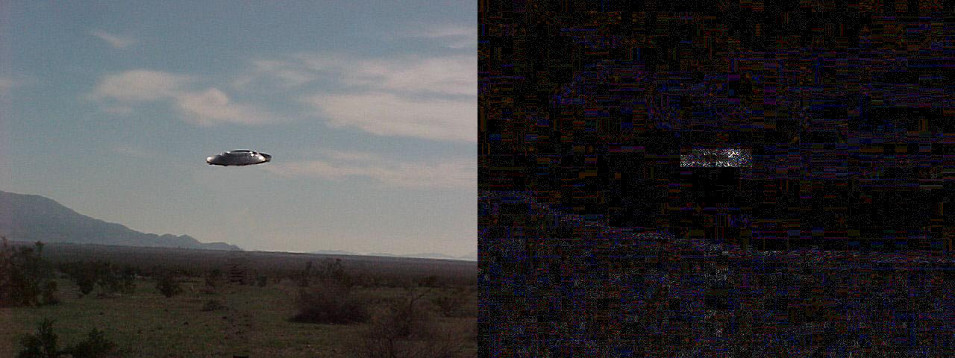
\includegraphics[width=16cm]{images/Libro-img053.jpg}
    \caption{Esempio di come i filtri possono rilevare un falso. Nell'immagine di destra si vede chiaramente un elemento estraneo applicato in un secondo momento all'immagine originaria.}
  \end{minipage}
\end{figure}

Esistono video ufficiali diffusi dall’aeronautica statunitense che mostrano oggetti volanti non identificati (UFO), autenticati come reali. Tuttavia, ciò non implica la presenza di alieni, ma semplicemente che si tratta di oggetti non riconosciuti. Secondo Paolo Attivissimo, noto debunker e membro del CICAP, questi video potrebbero essere un modo indiretto per segnalare attività di spionaggio di altre potenze, senza scatenare crisi diplomatiche. In passato, alcuni avvistamenti inizialmente inspiegabili si sono successivamente rivelati essere legati a progetti militari segreti, come nel caso dell’aereo F-117. Anche i militari spesso non conoscono i dettagli dei progetti top secret. In base ai dati del CUN (database italiano), il 3–5\% delle segnalazioni rimane inspiegabile dopo l’indagine, ma questo non implica che siano confermati UFO di origine extraterrestre.

Esistono studi contrastanti a quello dell’Università di Oxford, come quello dell’Università di Nottingham, rielaborando l’equazione di Drake, stima invece l’esistenza di circa 36 civiltà extraterrestri nella Via Lattea \endnote{\raggedright\url{https://iopscience.iop.org/article/10.3847/1538-4357/ab8225}}.

Dove sta la verità? Difficile dirlo con certezza. A volte dobbiamo accettare che certe domande non hanno (ancora) risposta e imparare a convivere con l’incertezza, piuttosto che cercare informazioni che confermino le nostre idee.
\end{mdframed}

Quindi la scienza non ha bias?

No, anche la scienza li ha, facciamo un esempio: Uno studio intende valutare l'efficacia di un
programma di perdita di peso per persone con diabete. Se lo studio si concentra solo sul numero di partecipanti che
completano il programma senza considerare altri fattori, come il tasso di abbandono o i cambiamenti nel comportamento
alimentare, potrebbe portare a conclusioni distorte. Ad esempio, se i partecipanti che non perdono peso tendono ad
abbandonare il programma e vengono così esclusi dai risultati, mentre quelli che hanno successo continuano, i risultati
potrebbero essere sbilanciati verso esiti più favorevoli.

Un altro esempio potrebbe essere uno studio sull'uso degli smartphone e i sintomi
muscoloscheletrici tra gli studenti delle scuole superiori. Se lo studio si basa su dati auto-segnalati dagli studenti
senza verificare l'accuratezza di tali dati, potrebbe esserci un bias informativo. Gli studenti
potrebbero sovrastimare o sottostimare il tempo trascorso al telefono, influenzando così i risultati dello studio.

Altre volte il campione utilizzato potrebbe essere troppo piccolo o poco rappresentativo perché prende solo una certa fascia di popolazione ad esempio per età, regione, sesso e così via. Chi più chi meno, siamo influenzati da questo provincialismo culturale, ovvero prendere il proprio piccolo mondo e chiamarlo Il Mondo! Affacciarsi dalla propria finestra e credere che quello sia Il Mondo. Se io sono convinto di qualcosa in base alla mia esperienza diretta, ma tu ne hai una percezione diversa, e nessuno dei due sta mentendo, come possiamo trovare un terreno comune di comprensione, se non attraverso un approccio che integri e valuti una molteplicità di esperienze e dati? Questo è parte del metodo scientifico.

Quindi come facciamo a sapere se una ricerca è affidabile? Soprattutto quando andiamo a leggere di una materia di cui
non abbiamo competenze?

Per prima cosa cerchiamo un articolo scientifico e per farlo possiamo affidarci a Google Scholar, fatto da Google e con
il medesimo funzionamento: \url{https://scholar.google.com}

Una volta fatta la ricerca, sulla colonna di sinistra, clicchiamo su “Articoli scientifici”.

I primi risultati tendono a essere quelli che l'algoritmo giudica più pertinenti, e una volta scelto l'articolo che ci interessa esaminiamo
la rivista. Riviste con un rigoroso processo di revisione paritaria sono generalmente considerate più affidabili, ma
questo può essere complicato da valutare anche con delle ricerche su Google per un non addetto ai lavori. Esiste un
indice che ci aiuta in questa analisi che è l'Impact Factor (IF). Questo indice riflette la media
annuale delle citazioni degli articoli pubblicati negli ultimi due anni in una determinata rivista, ed spesso
utilizzato come un indicatore dell'importanza relativa di una rivista nel suo campo; le riviste
con valori IF più alti sono considerate più importanti o prestigiose e potete trovarli su questo sito: \url{https://exaly.com/journals/if/}

Esistono diversi indicatori alternativi all'Impact Factor per valutare l'importanza e l'influenza di una rivista
scientifica. Ecco alcuni dei più noti:

\begin{itemize}
\item SCImago Journal Rank (SJR): Utilizza dati provenienti da Scopus e considera sia il numero di citazioni ricevute
che la prestigio delle riviste da cui provengono le citazioni. \url{https://www.scimagojr.com/journalrank.php} 
\item CiteScore: Calcolato anch'esso su dati Scopus, rappresenta il numero medio di citazioni ricevute in un anno da
articoli pubblicati nei tre anni precedenti.
\item Source Normalized Impact per Paper (SNIP): Misura l'impatto contestualizzato di una rivista, tenendo conto delle
caratteristiche del campo di ricerca.
\item Eigenfactor Score: Basato sul numero di volte in cui gli articoli della rivista sono stati citati negli ultimi
cinque anni, ma anche sulla "qualità" delle citazioni ricevute.
\end{itemize}

Non avendo competenze per valutare autonomamente uno studio, possiamo delegare questa responsabilità alla rivista
scientifica che sceglieremo tramite l'impact score, un indice basato sulle citazioni. Un alto numero di citazioni può indicare che lo studio ha avuto un impatto nel campo, ma non necessariamente che sia stato considerato valido da tutti i ricercatori. Valutare la serietà della rivista può essere un buon primo passo, ma non garantisce da solo l’affidabilità dello studio, poiché anche le riviste autorevoli possono occasionalmente pubblicare ricerche con limiti metodologici. Un altro controllo molto veloce e che aumenta la credibilità di uno
studio è vedere quante volte l'articolo è stato citato da altre ricerche. Se un articolo è stato
citato molte volte in altre ricerche vuol dire che persone competenti in quella materia hanno ritenuto valido questo
studio, analizzandolo, meglio di come potremmo fare noi outsider. Potete vedere le citazioni in Google Scholar, già dai
risultati di ricerca, prima ancora di entrare dentro l'articolo vero e proprio.

\begin{mdframed}[linewidth=1pt]
Giornali
La cronaca andrebbe riformata per ridurre l’enfasi su episodi isolati e aumentare l’attenzione ai dati e ai trend di lungo periodo, così da offrire una rappresentazione più equilibrata della realtà. Ciò che dovrebbe interessarci, e su cui dovremmo concentrare l'attenzione, sono le statistiche e i dati oggettivi riguardanti una determinata area, piuttosto che i singoli episodi di violenza o tragedie personali. Un approccio basato sulle statistiche ci permetterebbe di capire meglio l'andamento della sicurezza pubblica, evidenziando trend e problematiche reali che meritano attenzione collettiva e soluzioni concrete.

I criteri quantitativi possono aiutare a bilanciare la rilevanza delle notizie, ma dovrebbero essere integrati con valutazioni qualitative, come il potenziale impatto sociale o il valore informativo dell’evento. Bisognerebbe chiedersi: quante persone sono realmente coinvolte o interessate da questa vicenda? Se la risposta è solo una manciata di persone (ad esempio, un caso isolato di aggressione), potrebbe essere opportuno modulare lo spazio mediatico, pur riconoscendo il valore intrinseco di ogni singola storia. Al contrario, questioni che toccano la vita di milioni di persone, come casi di corruzione politica o temi d'interesse pubblico, meritano maggiore visibilità.

Si potrebbe obiettare che la cronaca ci informa dei rischi reali che potremmo incontrare. I media però possono talvolta enfatizzare eventi rari ma emotivamente forti, come gli omicidi, dando un’impressione distorta del rischio reale, mentre fenomeni più comuni ma letali, come gli incidenti stradali, ricevono spesso meno attenzione proporzionale.

L’aspetto più subdolo e crudele della cronaca, forse anche in modo involontario, è che finisce per indurre le persone, che vivono in un Paese tra i più sicuri al mondo, a condurre un’esistenza dominata dalla paura.
\end{mdframed}

Altri punti:
\begin{itemize}
\item Ricerca di conflitti di interesse: Solitamente in fondo alla ricerca vengono citati anche i finanziatori. Se tra i finanziatori di uno studio che osserva benefici di un integratore compaiono aziende che lo producono, è importante valutare con maggiore cautela i risultati, poiché potrebbe esserci un potenziale conflitto d’interessi, anche se ciò non invalida automaticamente le conclusioni dello studio.
\item Verifica gli autori: Controlla le qualifiche degli autori e la loro affiliazione istituzionale. Gli autori
rispettabili e le istituzioni rinomate possono aumentare la credibilità della ricerca.
\item Controlla le citazioni: Uno studio che cita fonti pertinenti e attuali dimostra che gli autori hanno considerato il contesto della loro ricerca.
\item Analizza i dati e i risultati: I risultati dovrebbero essere presentati in modo chiaro e supportati dai dati.
Attenzione a qualsiasi affermazione che sembra troppo buona per essere vera o non supportata da prove.
\item Consulta esperti: Se possibile, discuti la ricerca con colleghi o esperti nel campo per ottenere la loro opinione
sulla validità dello studio.
\end{itemize}

Noterai subito che gli articoli scientifici sono numerosi e in continuo aumento di anno in anno, come posso leggere così
tante pagine per ogni dubbio che ho? La scienza sta diventando sempre più accessibile, infatti gli articoli sono
strutturati in modo da mettere all'inizio un abstract, che solitamente è fatto da pochi paragrafi,
che sostanzialmente è un riassunto. Negli ultimi anni sempre più articoli inseriscono gli highlights, che sono i punti
principali, per renderci ancora più facile e veloce avere un idea di massima di cosa parla
l'articolo.

Le meta-analisi sono strumenti particolarmente utili quando si vogliono sintetizzare i risultati di più studi su una stessa domanda di ricerca, offrendo una visione più ampia e una stima complessiva più solida. Questo processo statistico valuta
l'efficacia clinica calcolando una stima combinata ponderata degli interventi, basata su almeno
due studi separati. Le meta-analisi sono strumenti potenti che possono migliorare la precisione e, in alcuni casi, risolvere controversie
derivanti da risultati contrastanti e rispondere a domande che non possono essere affrontate da singoli studi. Inoltre,
aiutano a standardizzare e migliorare la qualità delle revisioni sistematiche attraverso linee guida come la
dichiarazione PRISMA.

Quindi se leggete un articolo su internet che parla di ricerche, controllate se avete gli estremi di questo studio in
modo che possiate analizzarlo. In modo da poter essere critici anche quando si parla di numeri e grafici. Un libro che mi ha aiutato a capire quanto anche dati e numeri, se presentati o visualizzati in modo selettivo, possano suggerire interpretazioni fuorvianti, è stato Factfulness\endnote{\raggedright\url{https://www.amazon.it/dp/B07BMN2N6D/}}, dove anche
valori corretti, se elaborarli o visualizzati in un certo modo, possono far assumere un concetto molto diverso.

\needspace{4cm}
\begin{figure}[H]
    \begin{minipage}{0.3\textwidth}
        \centering
        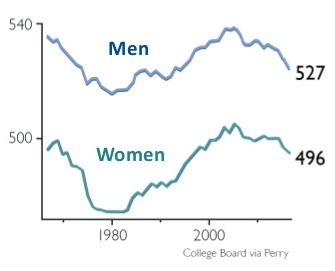
\includegraphics[width=\linewidth]{images/Libro-img003.jpg}
    \end{minipage}
    \hfill
    \begin{minipage}{0.3\textwidth}
        \centering
        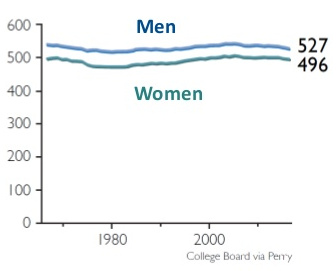
\includegraphics[width=\linewidth]{images/Libro-img005.jpg}
    \end{minipage}
    \hfill
    \begin{minipage}{0.3\textwidth}
        \centering
        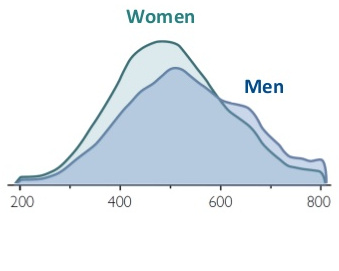
\includegraphics[width=\linewidth]{images/Libro-img004.jpg}
    \end{minipage}
\end{figure}

Questi tre grafici che ritroviamo sul libro mostrano i risultati di test di matematica divisi tra uomini e donne. Se
guardiamo il primo grafico, dove sono mostrate le medie dei test di matematica nei vari anni, vediamo che le donne
conseguono un punteggio decisamente inferiore rispetto agli uomini, ma è davvero così? Spostiamoci sul secondo grafico: i dati sono gli stessi, ma cambiando la scala dell’asse Y da 450–540 a 0–600, la differenza tra i punteggi di uomini e donne appare visivamente molto ridotta. Come vengono presentati i dati può influenzare la percezione, pur non modificando i numeri reali. Factfulness spiega come le medie possano essere fuorvianti. I primi due grafici mostrano i risultati medi di ogni
anno, mentre nel terzo vediamo tutti i risultati, senza medie, di un solo anno, il 2016. Notiamo come i dati sono quasi
sovrapponibili, non mostrando significative differenze tra uomini e donne.

Quando una storia parla di un divario, creando due gruppi separati con uno spazio nel mezzo, fate attenzione! Spesso la
realtà non è polarizzata, non c'è bianco o nero, ma una grande zona grigia. Fate attenzione alle
medie e cercate le dispersioni, potrebbero sovrapporsi e non mostrare le differenze indicate dalle medie. Riconoscete
quando vengono confrontati due estremi, di gruppi, paesi, persone, sesso, ecc… ci saranno elementi in cima e in
fondo, ma la verità sta spesso nel mezzo, dove c'è la maggioranza.

Questo libro inoltre, in controtendenza con l'idea ampiamente diffusa che il mondo sta lentamente andando in
rovina, mostra in realtà una tendenza contraria. Alcuni ricercatori come Max Roser, dell'Università di Oxford tramite
ourworldindata.org, Anna Rosling Rönnlund, Hans Rosling e Ola Rosling, ci mostrano anni di dati che danno una visione
del mondo molto più ottimistica sotto vari punti di vista. Vediamone alcuni:

\begin{table}[H]
\centering
\begin{tabular}{cc}
  \begin{subfigure}{0.5\textwidth}
    \centering
    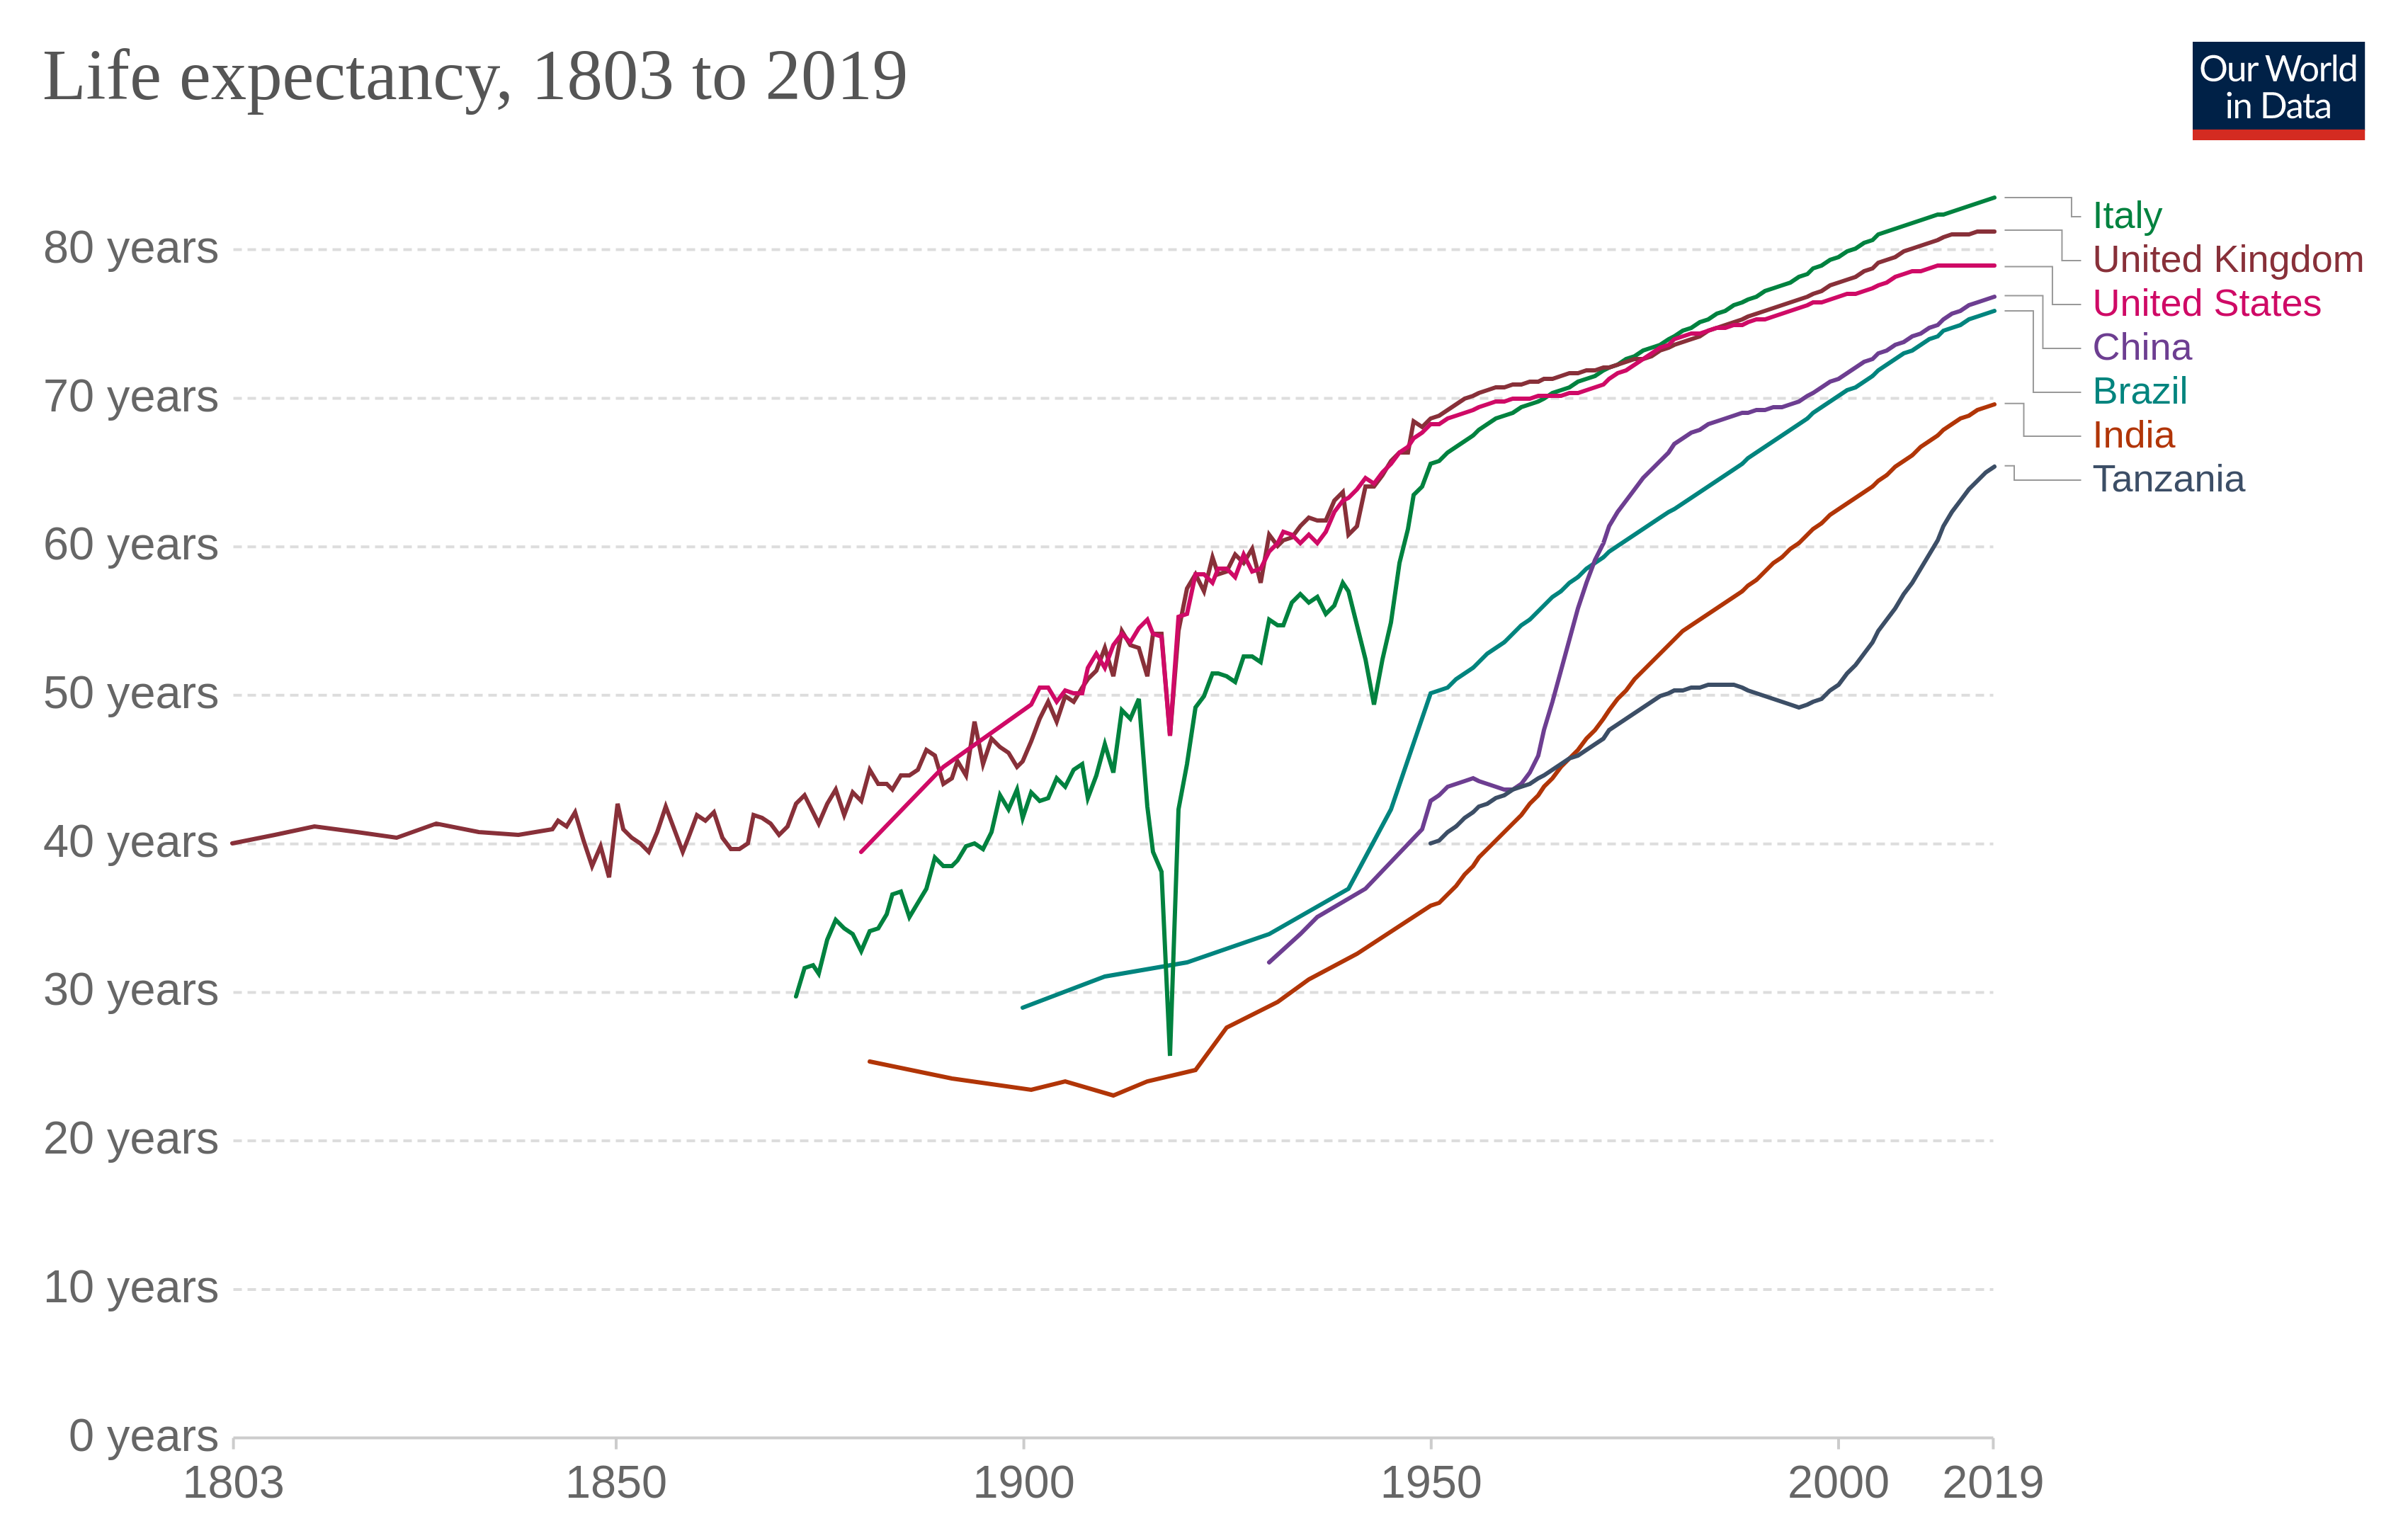
\includegraphics[width=0.8\linewidth]{images/Libro-img006.png}
    \caption{L'aspettativa di vita è raddoppiata dal 1800 al 2011
Credits: \raggedright\url{https://ourworldindata.org/grapher/life-expectancy?country=BRA+CHN+IND+TZA+GBR+USA} Source: Riley (2005), Clio
Infra (2015), and UN Population Division (2019) OurWorldInData.org/life-expectancy • CC BY}
  \end{subfigure}
  &
  \begin{subfigure}{0.5\textwidth}
    \centering
    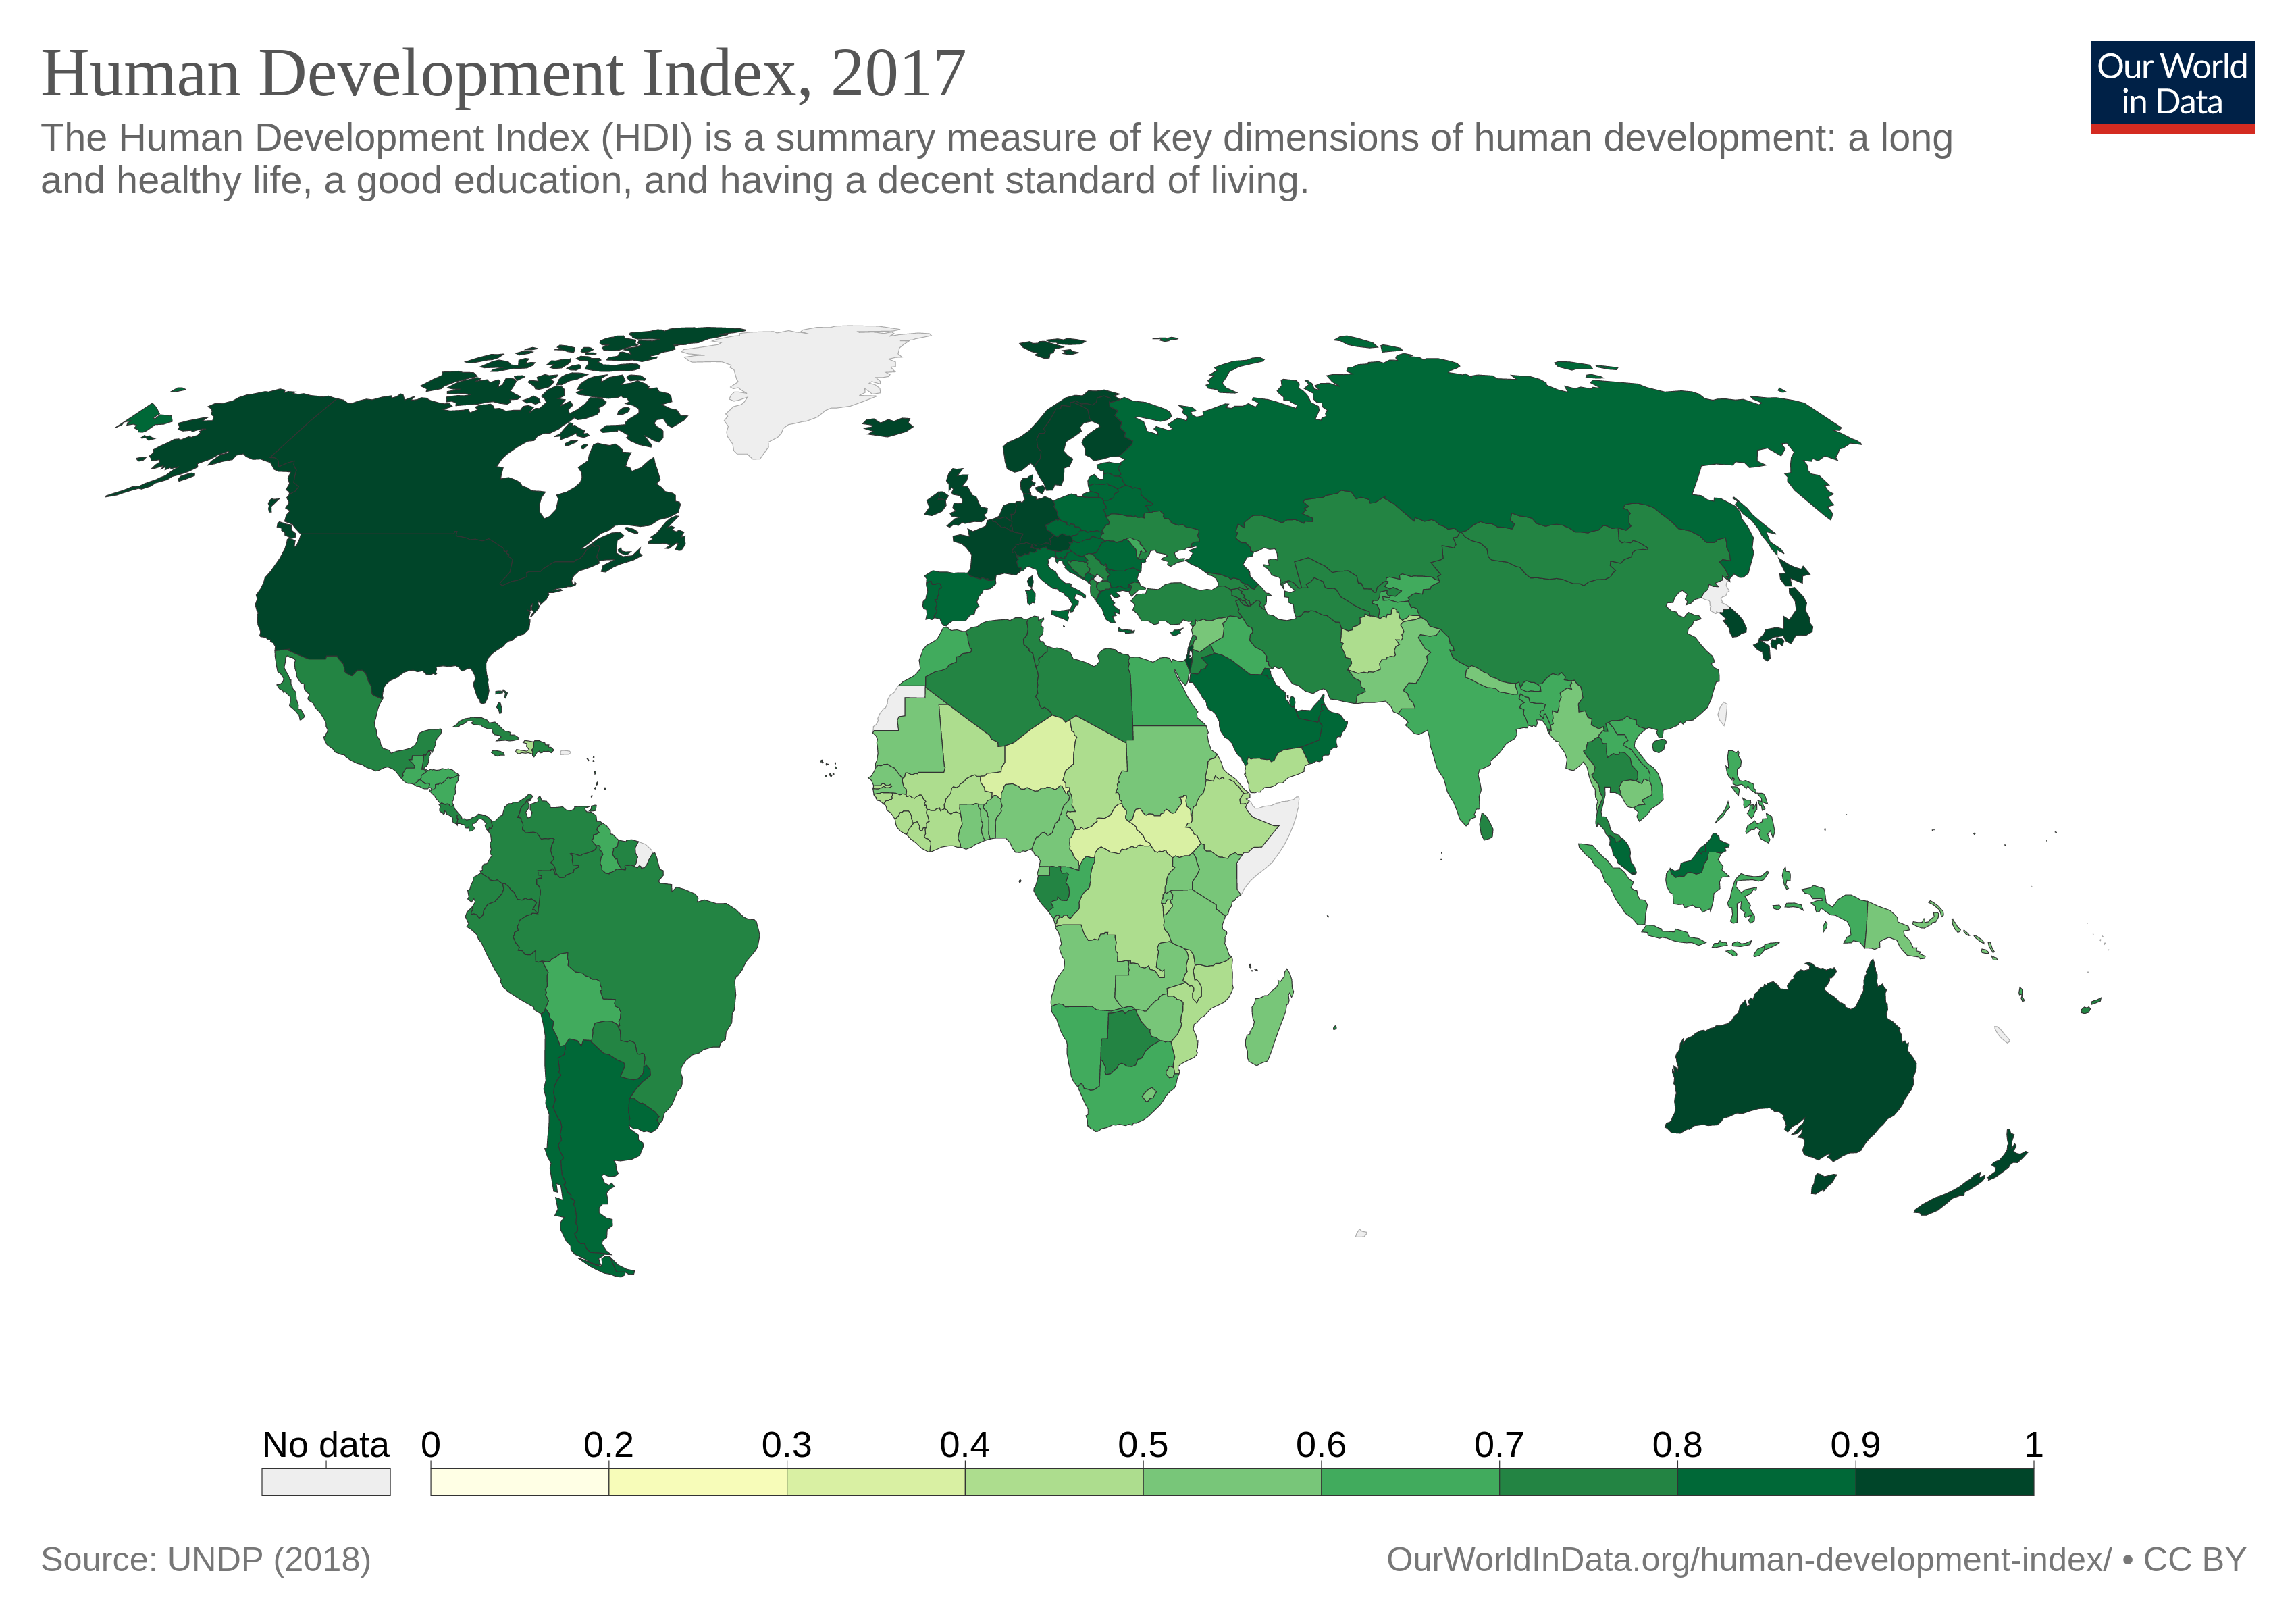
\includegraphics[width=0.8\linewidth]{images/Libro-img007.png}
    \caption{L'indice dello sviluppo umano (HDI) delle nazioni unite è in continua crescita, meno del 10\% delle
persone sulla terra vive in condizioni di povertà assoluta (nel 1900 era l'80\%)
Credits: \raggedright\url{https://ourworldindata.org/grapher/human-development-index?year=earliest}}
  \end{subfigure}
\end{tabular}
\end{table}

\begin{table}[H]
\centering
\begin{tabular}{cc}
  \begin{subfigure}{0.5\textwidth}
    \centering
    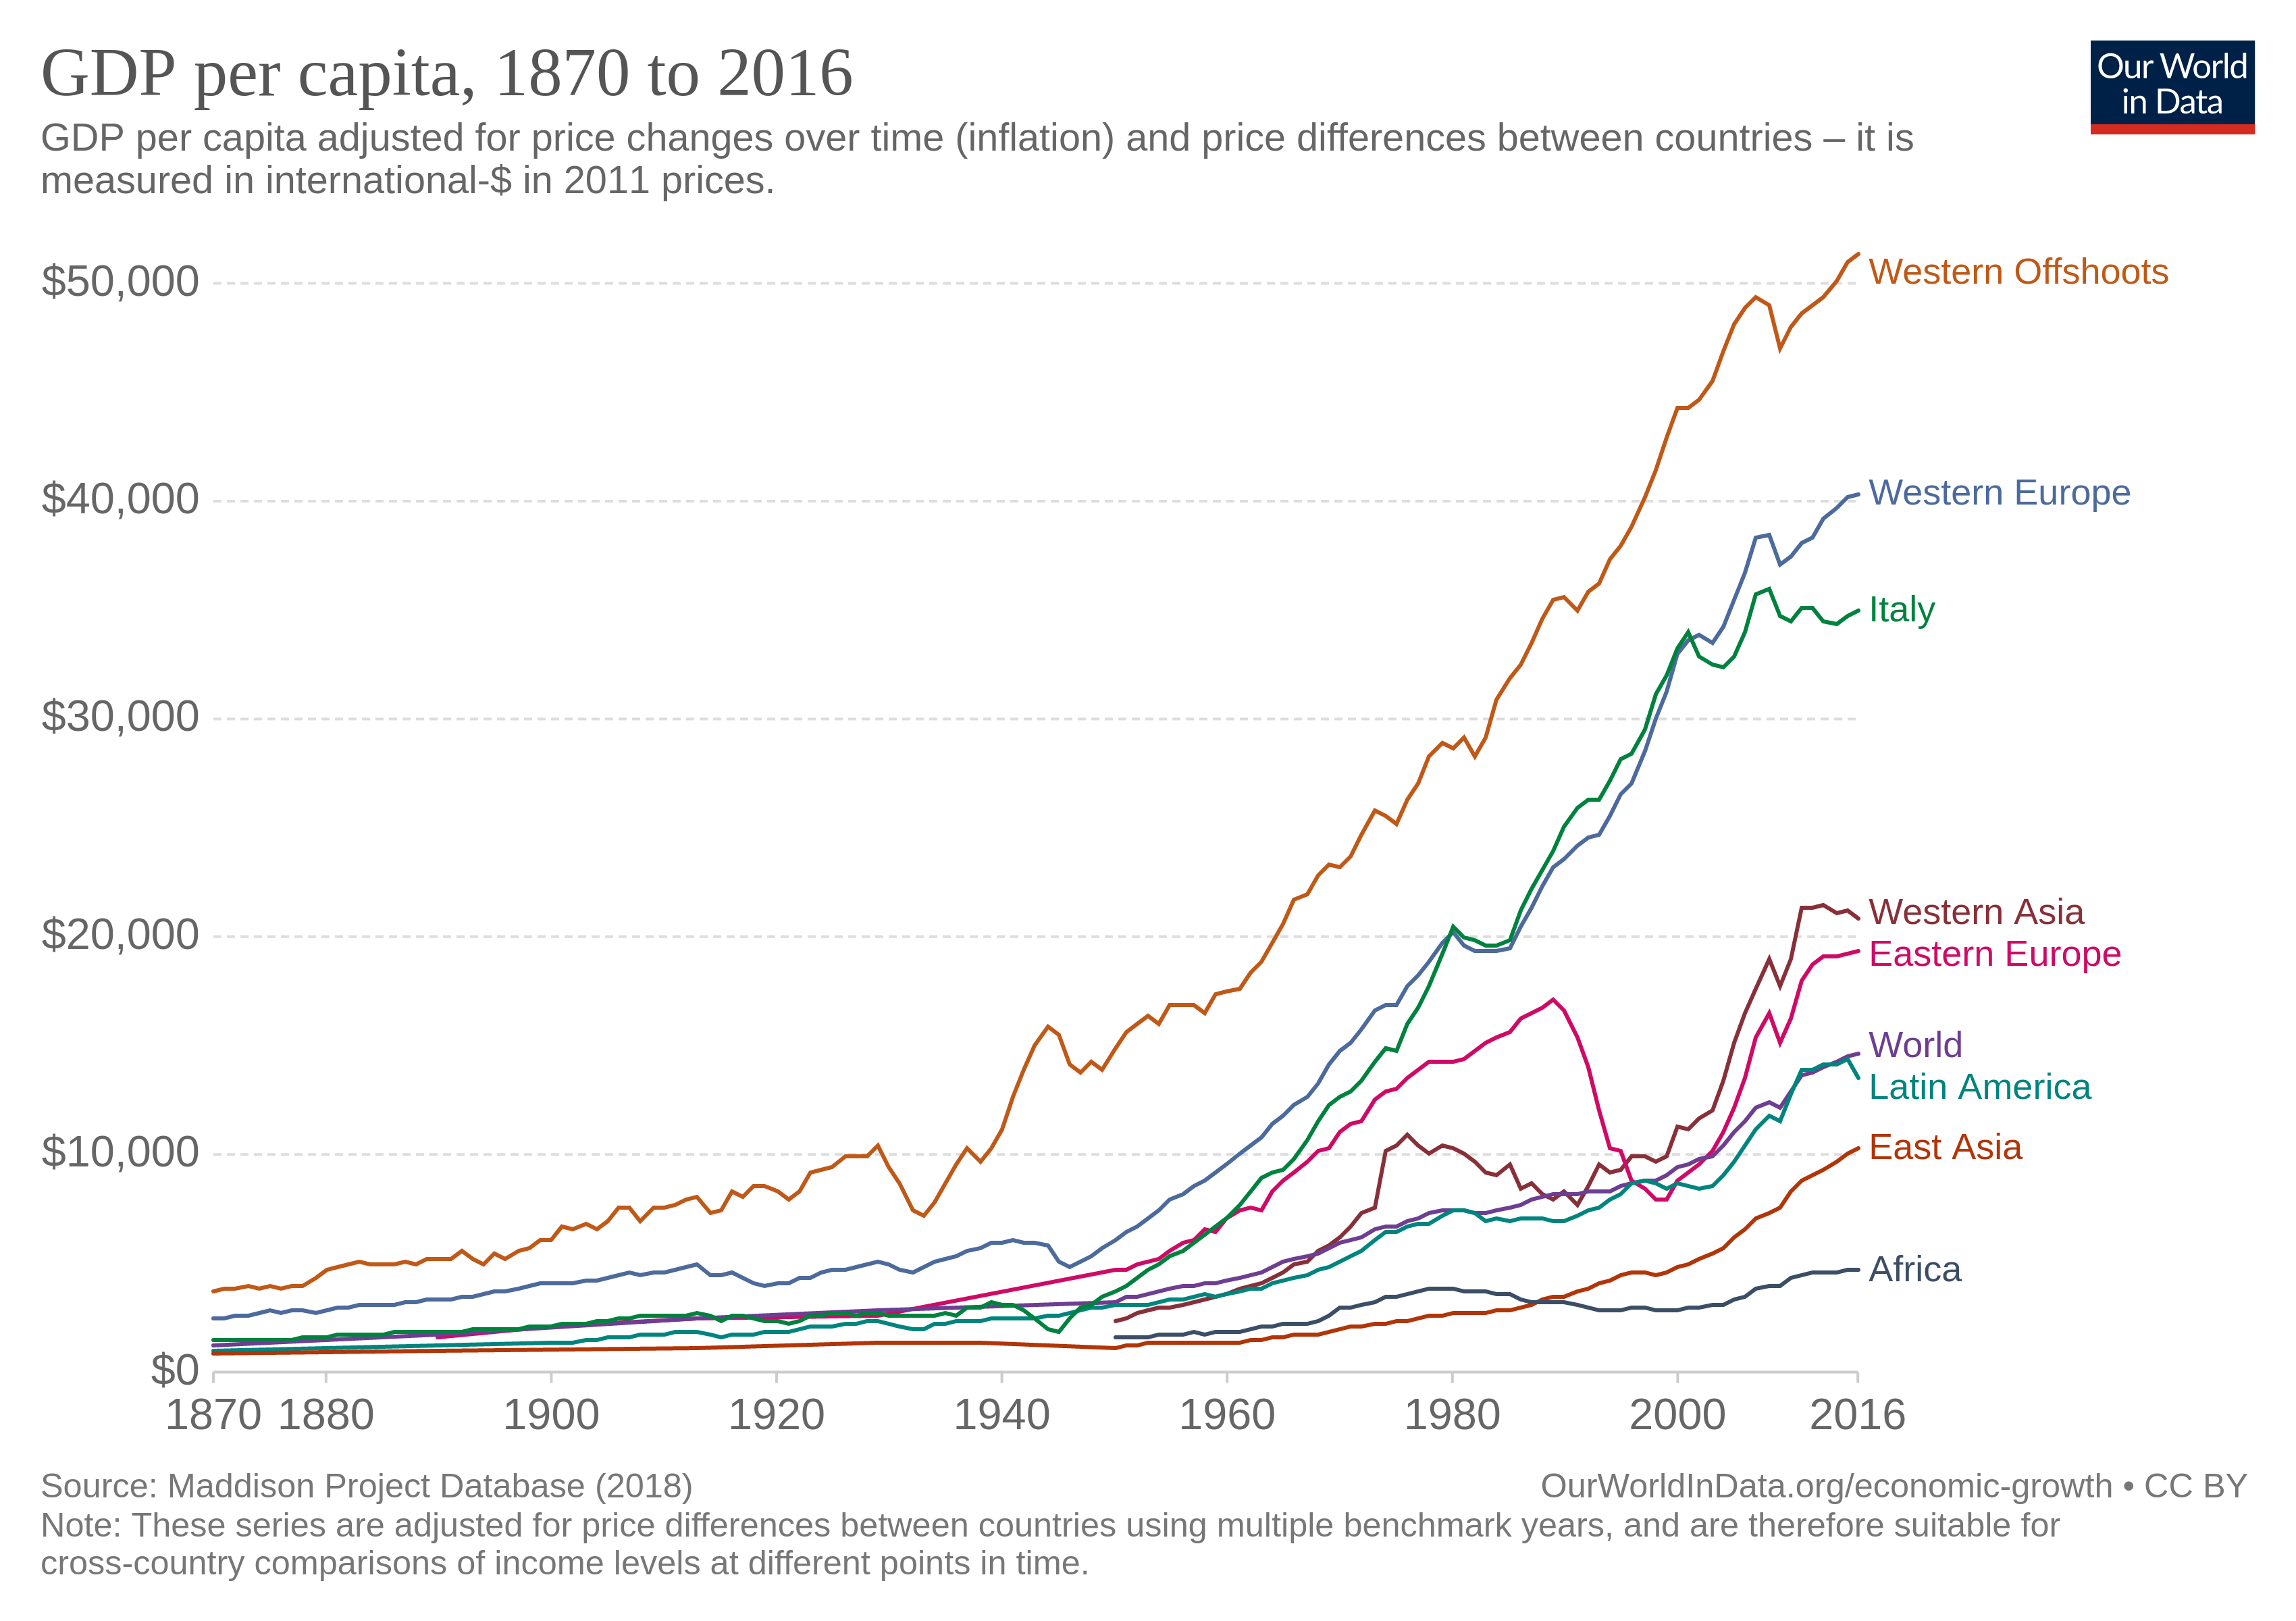
\includegraphics[width=0.8\linewidth]{images/Libro-img008.png}
    \caption{Il PIL è in continuo aumento
Credits: \raggedright\url{https://ourworldindata.org/grapher/average-real-gdp-per-capita-across-countries-and-regions}}
  \end{subfigure}
  &
  \begin{subfigure}{0.5\textwidth}
    \centering
    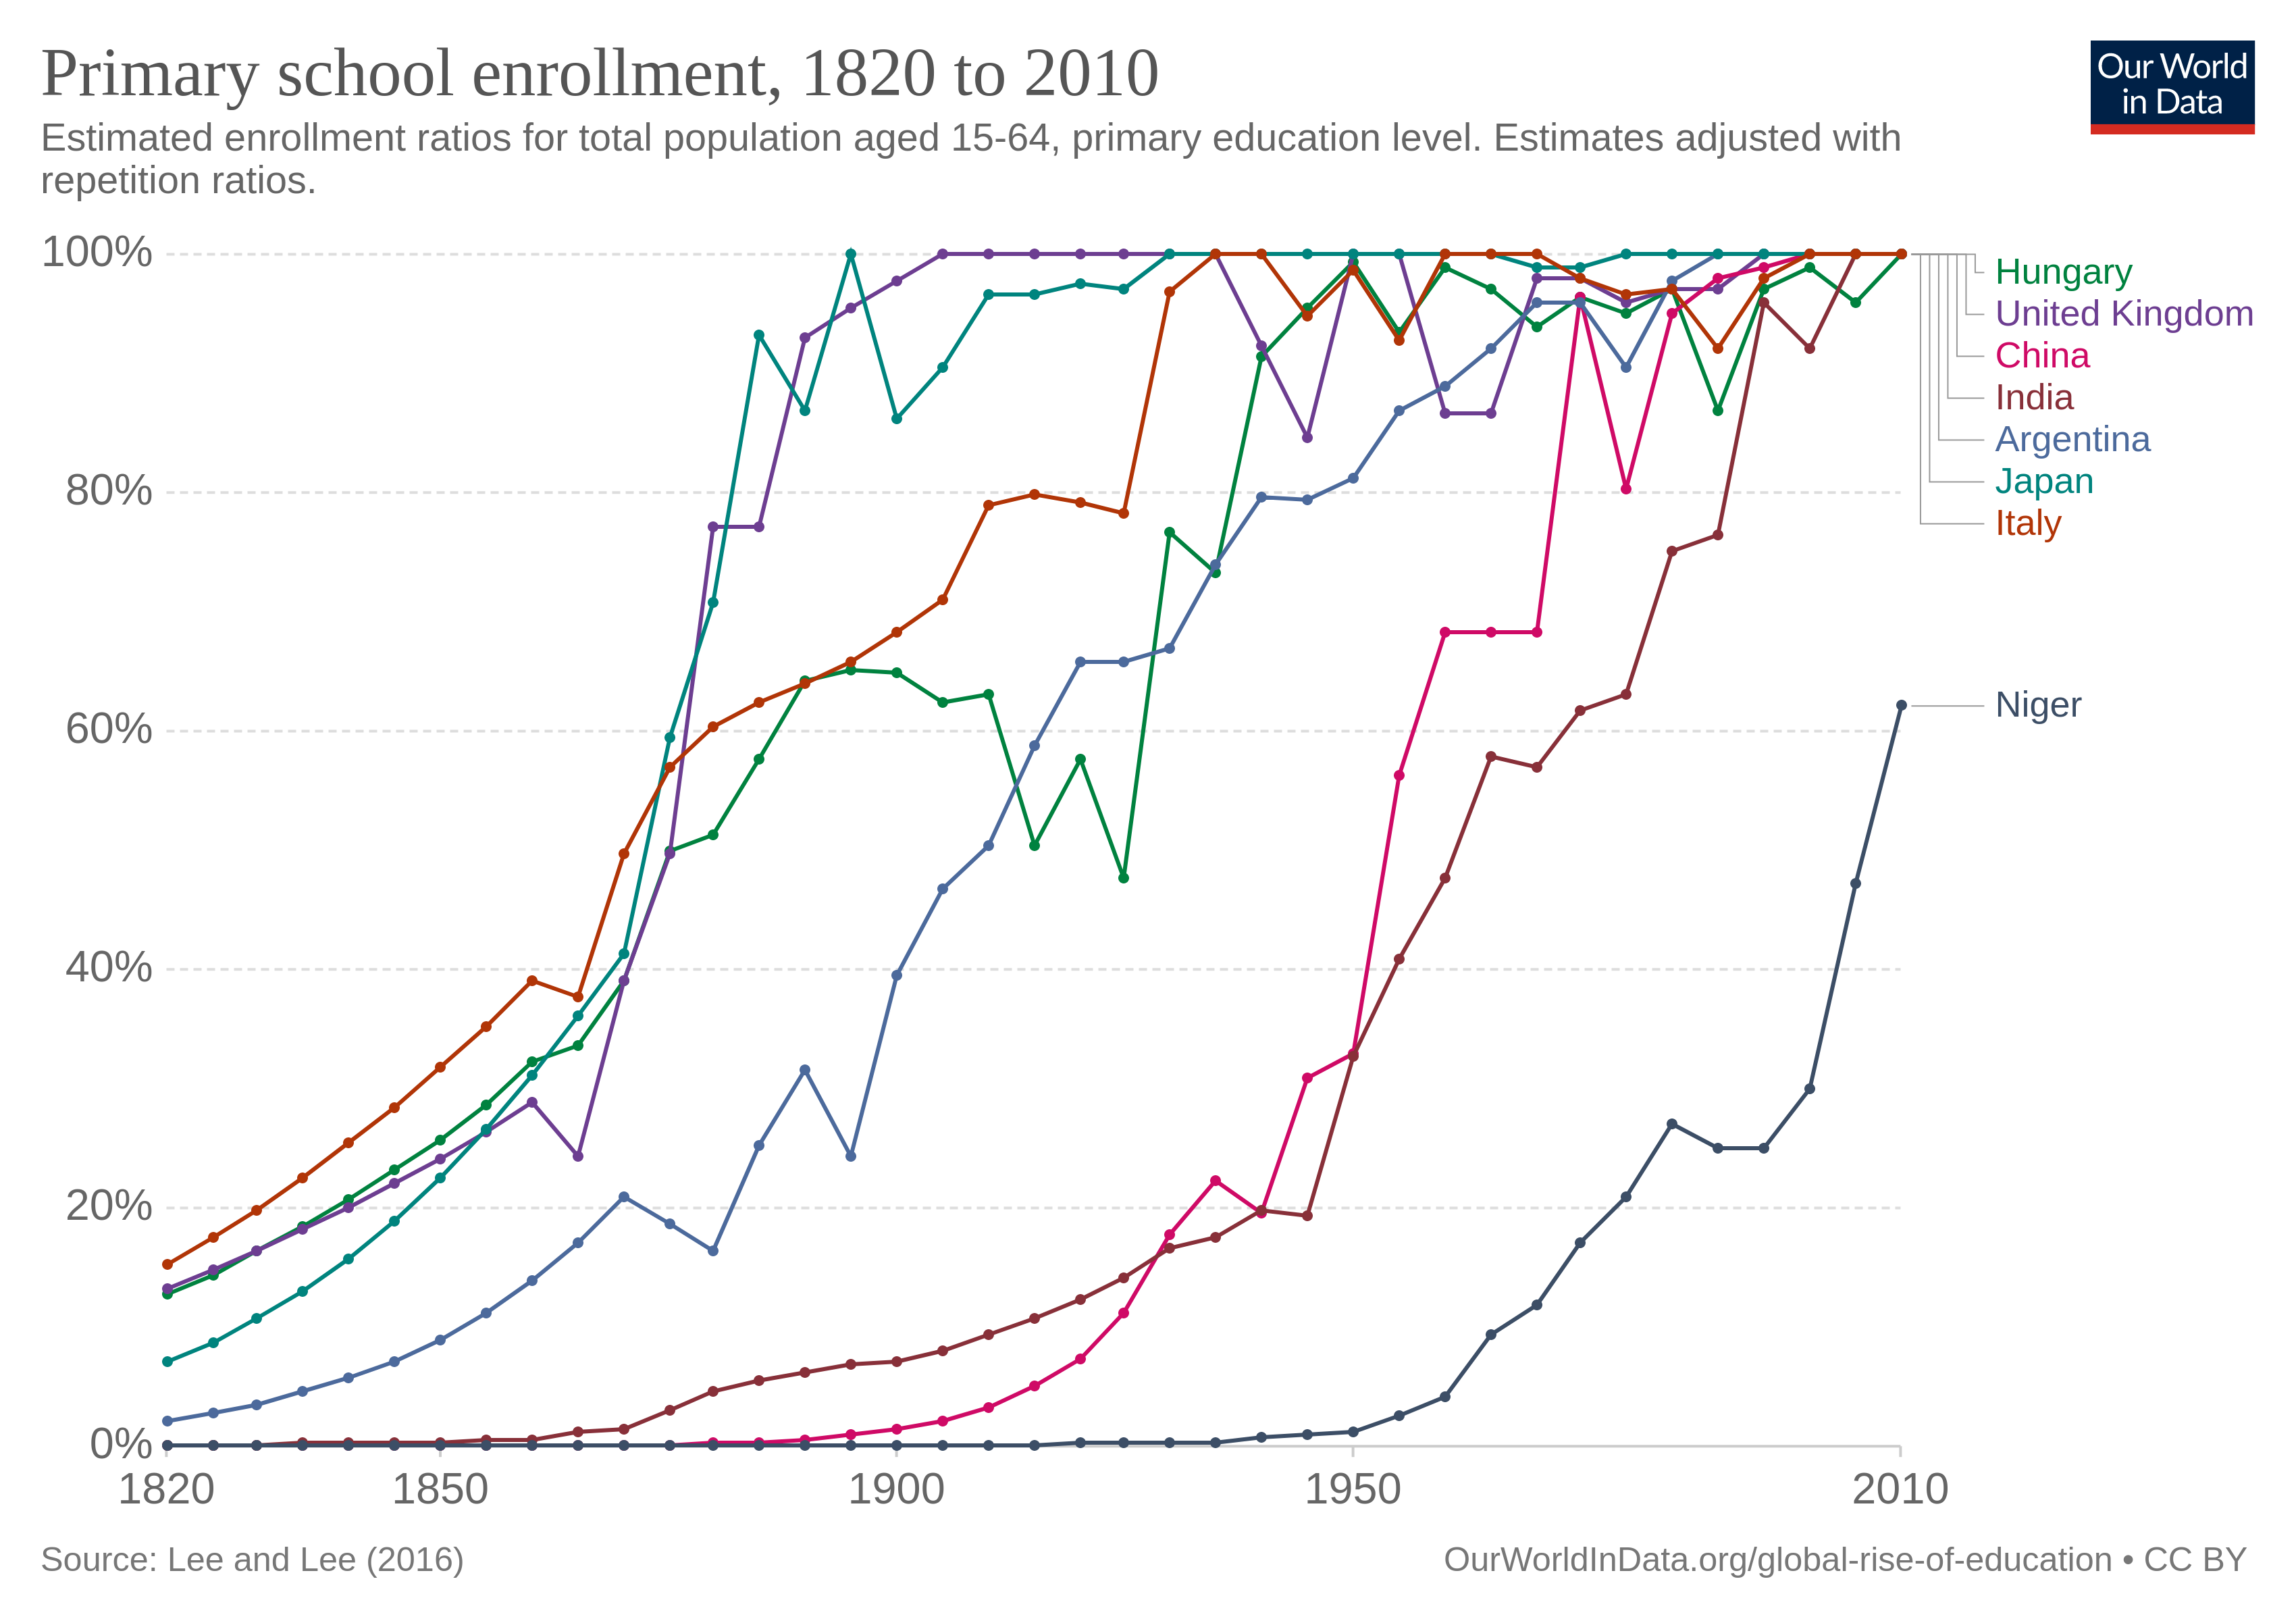
\includegraphics[width=0.8\linewidth]{images/Libro-img009.png}
    \caption{Migliora la ridistribuzione della ricchezza e il conseguente aumento dell'istruzione
Credits : \raggedright\url{https://ourworldindata.org/global-education\#school-enrollment-and-attendance}}
  \end{subfigure}
\end{tabular}
\end{table}

\begin{table}[H]
\centering
\begin{tabular}{cc}
  \begin{subfigure}{0.5\textwidth}
    \centering
    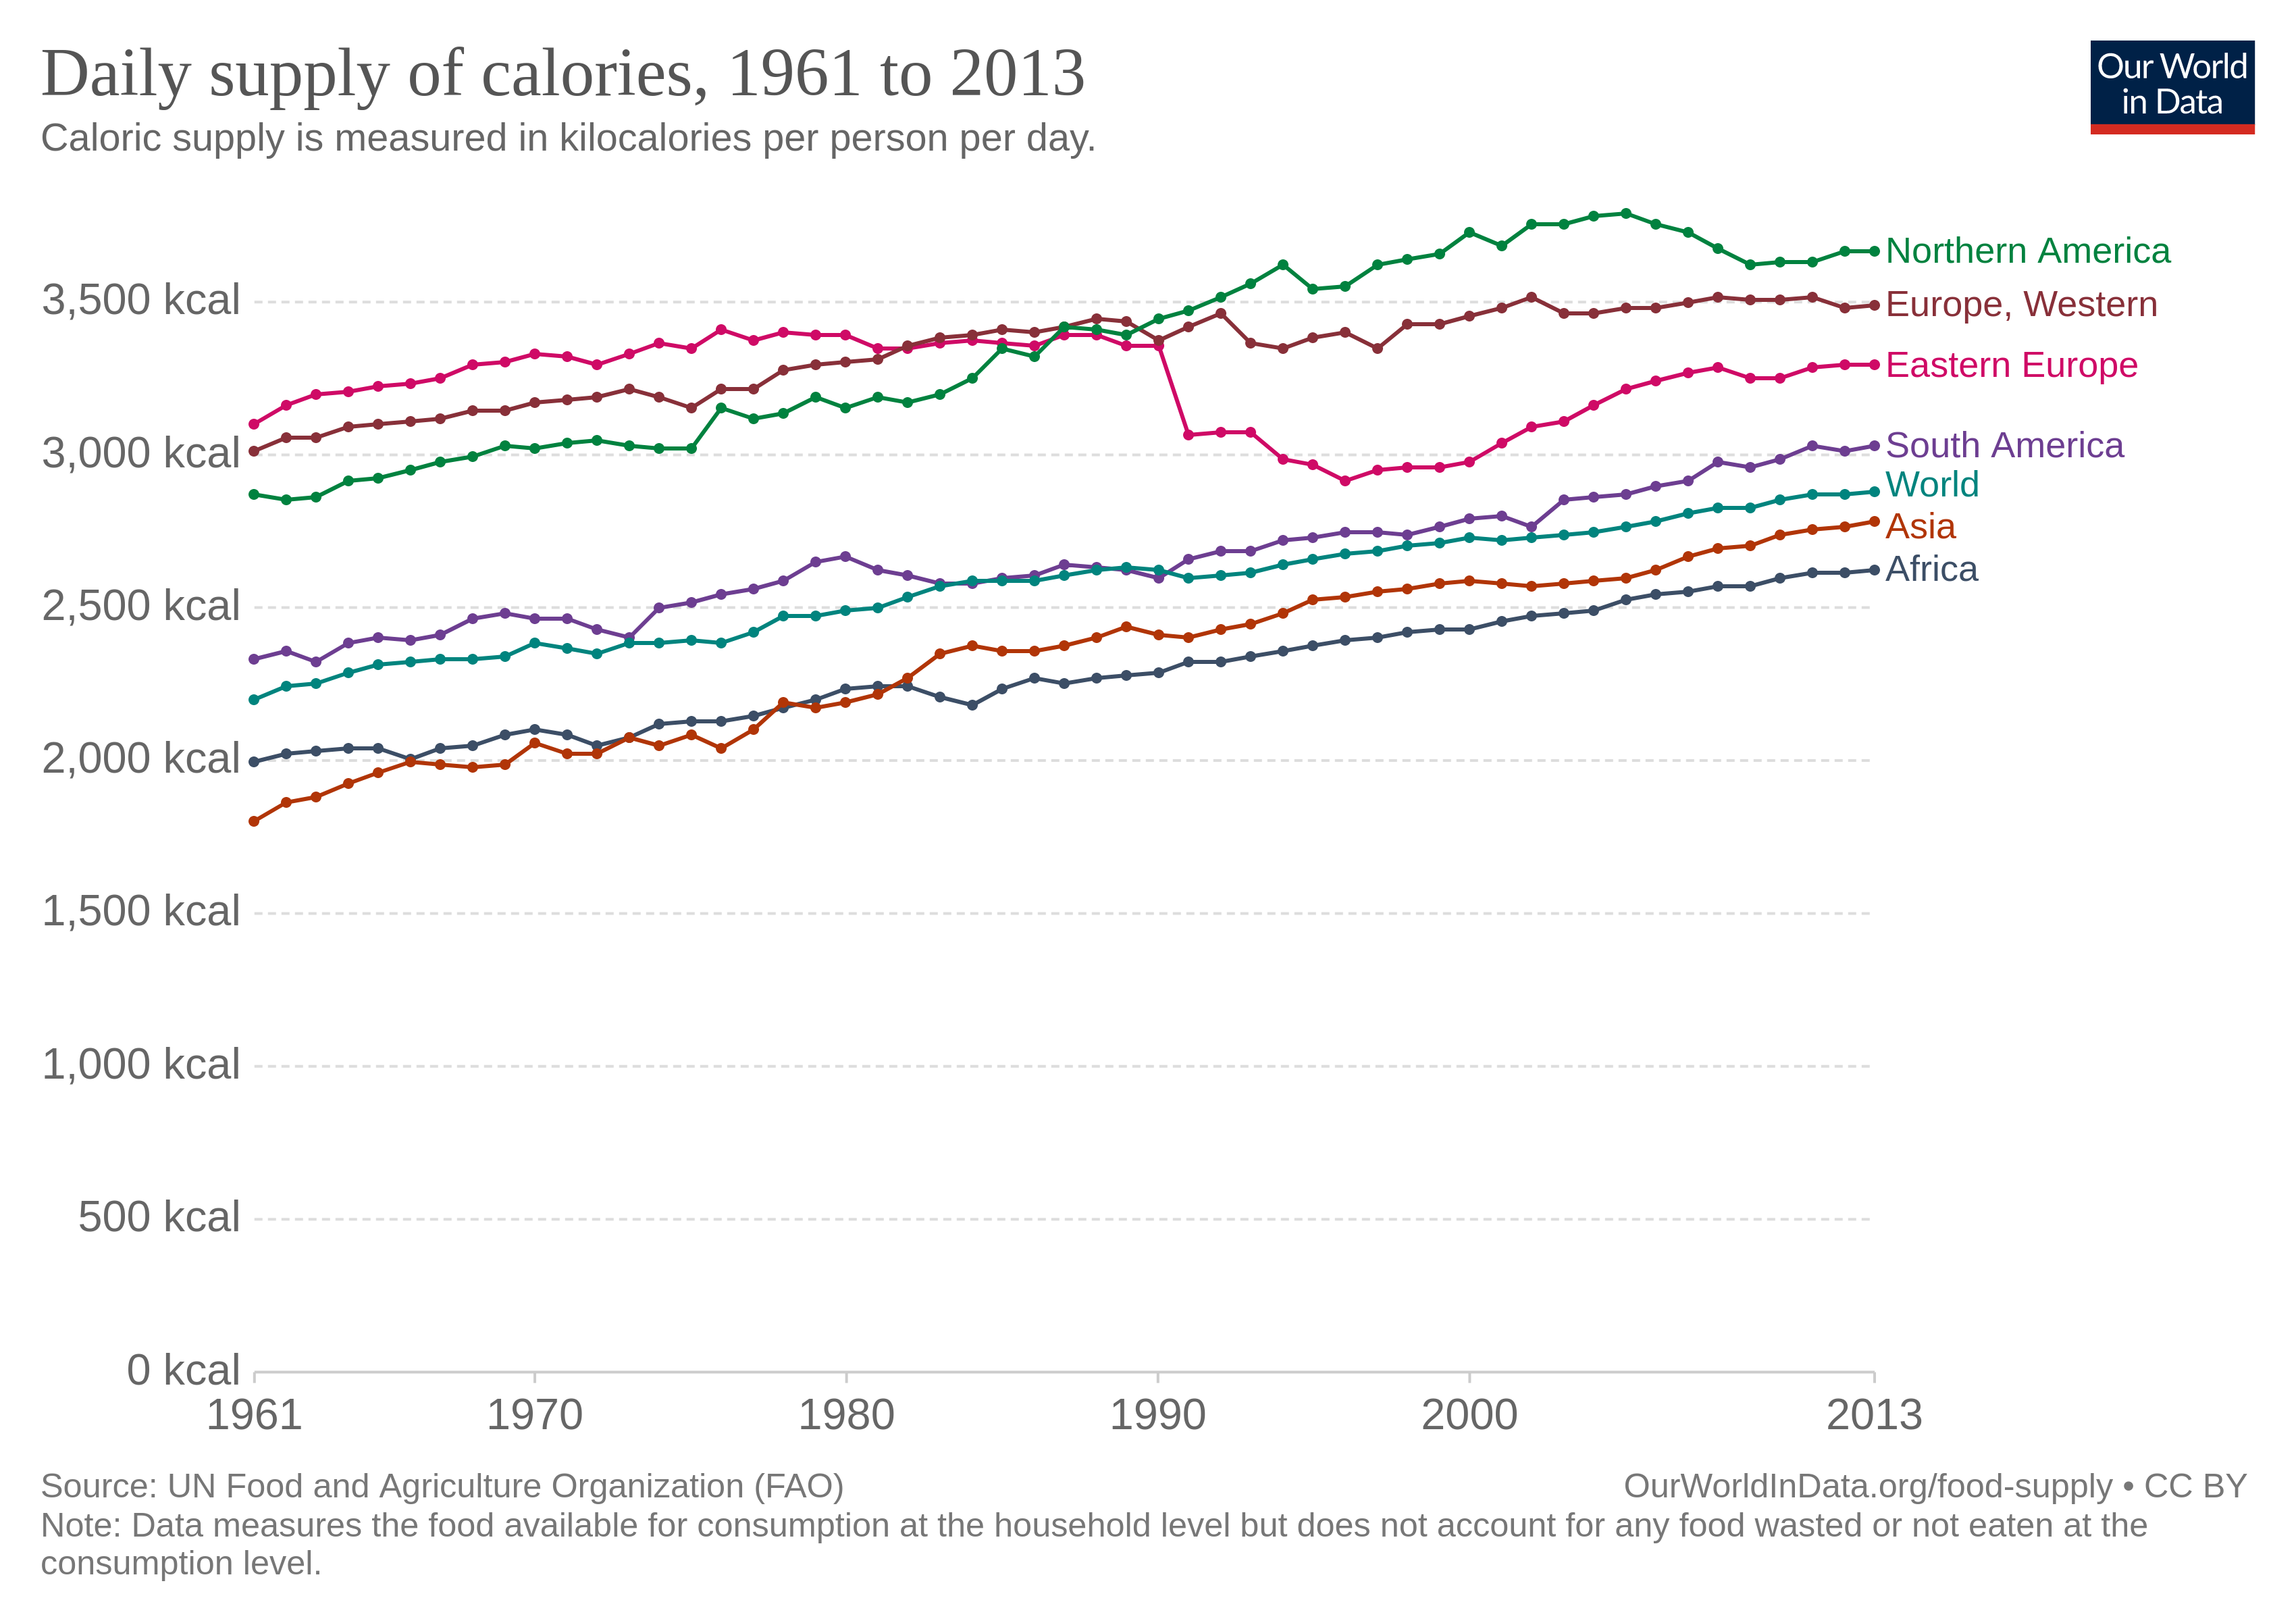
\includegraphics[width=0.8\linewidth]{images/Libro-img010.png}
    \caption{Aumenta la quantità di cibo prodotto
Credits: \raggedright\url{https://ourworldindata.org/wp-content/uploads/datamaps/kcalPerCapita\_since1961\_FAO/kcalPerCapita\_since1961\_FAO.html}}
  \end{subfigure}
  &
  \begin{subfigure}{0.5\textwidth}
    \centering
    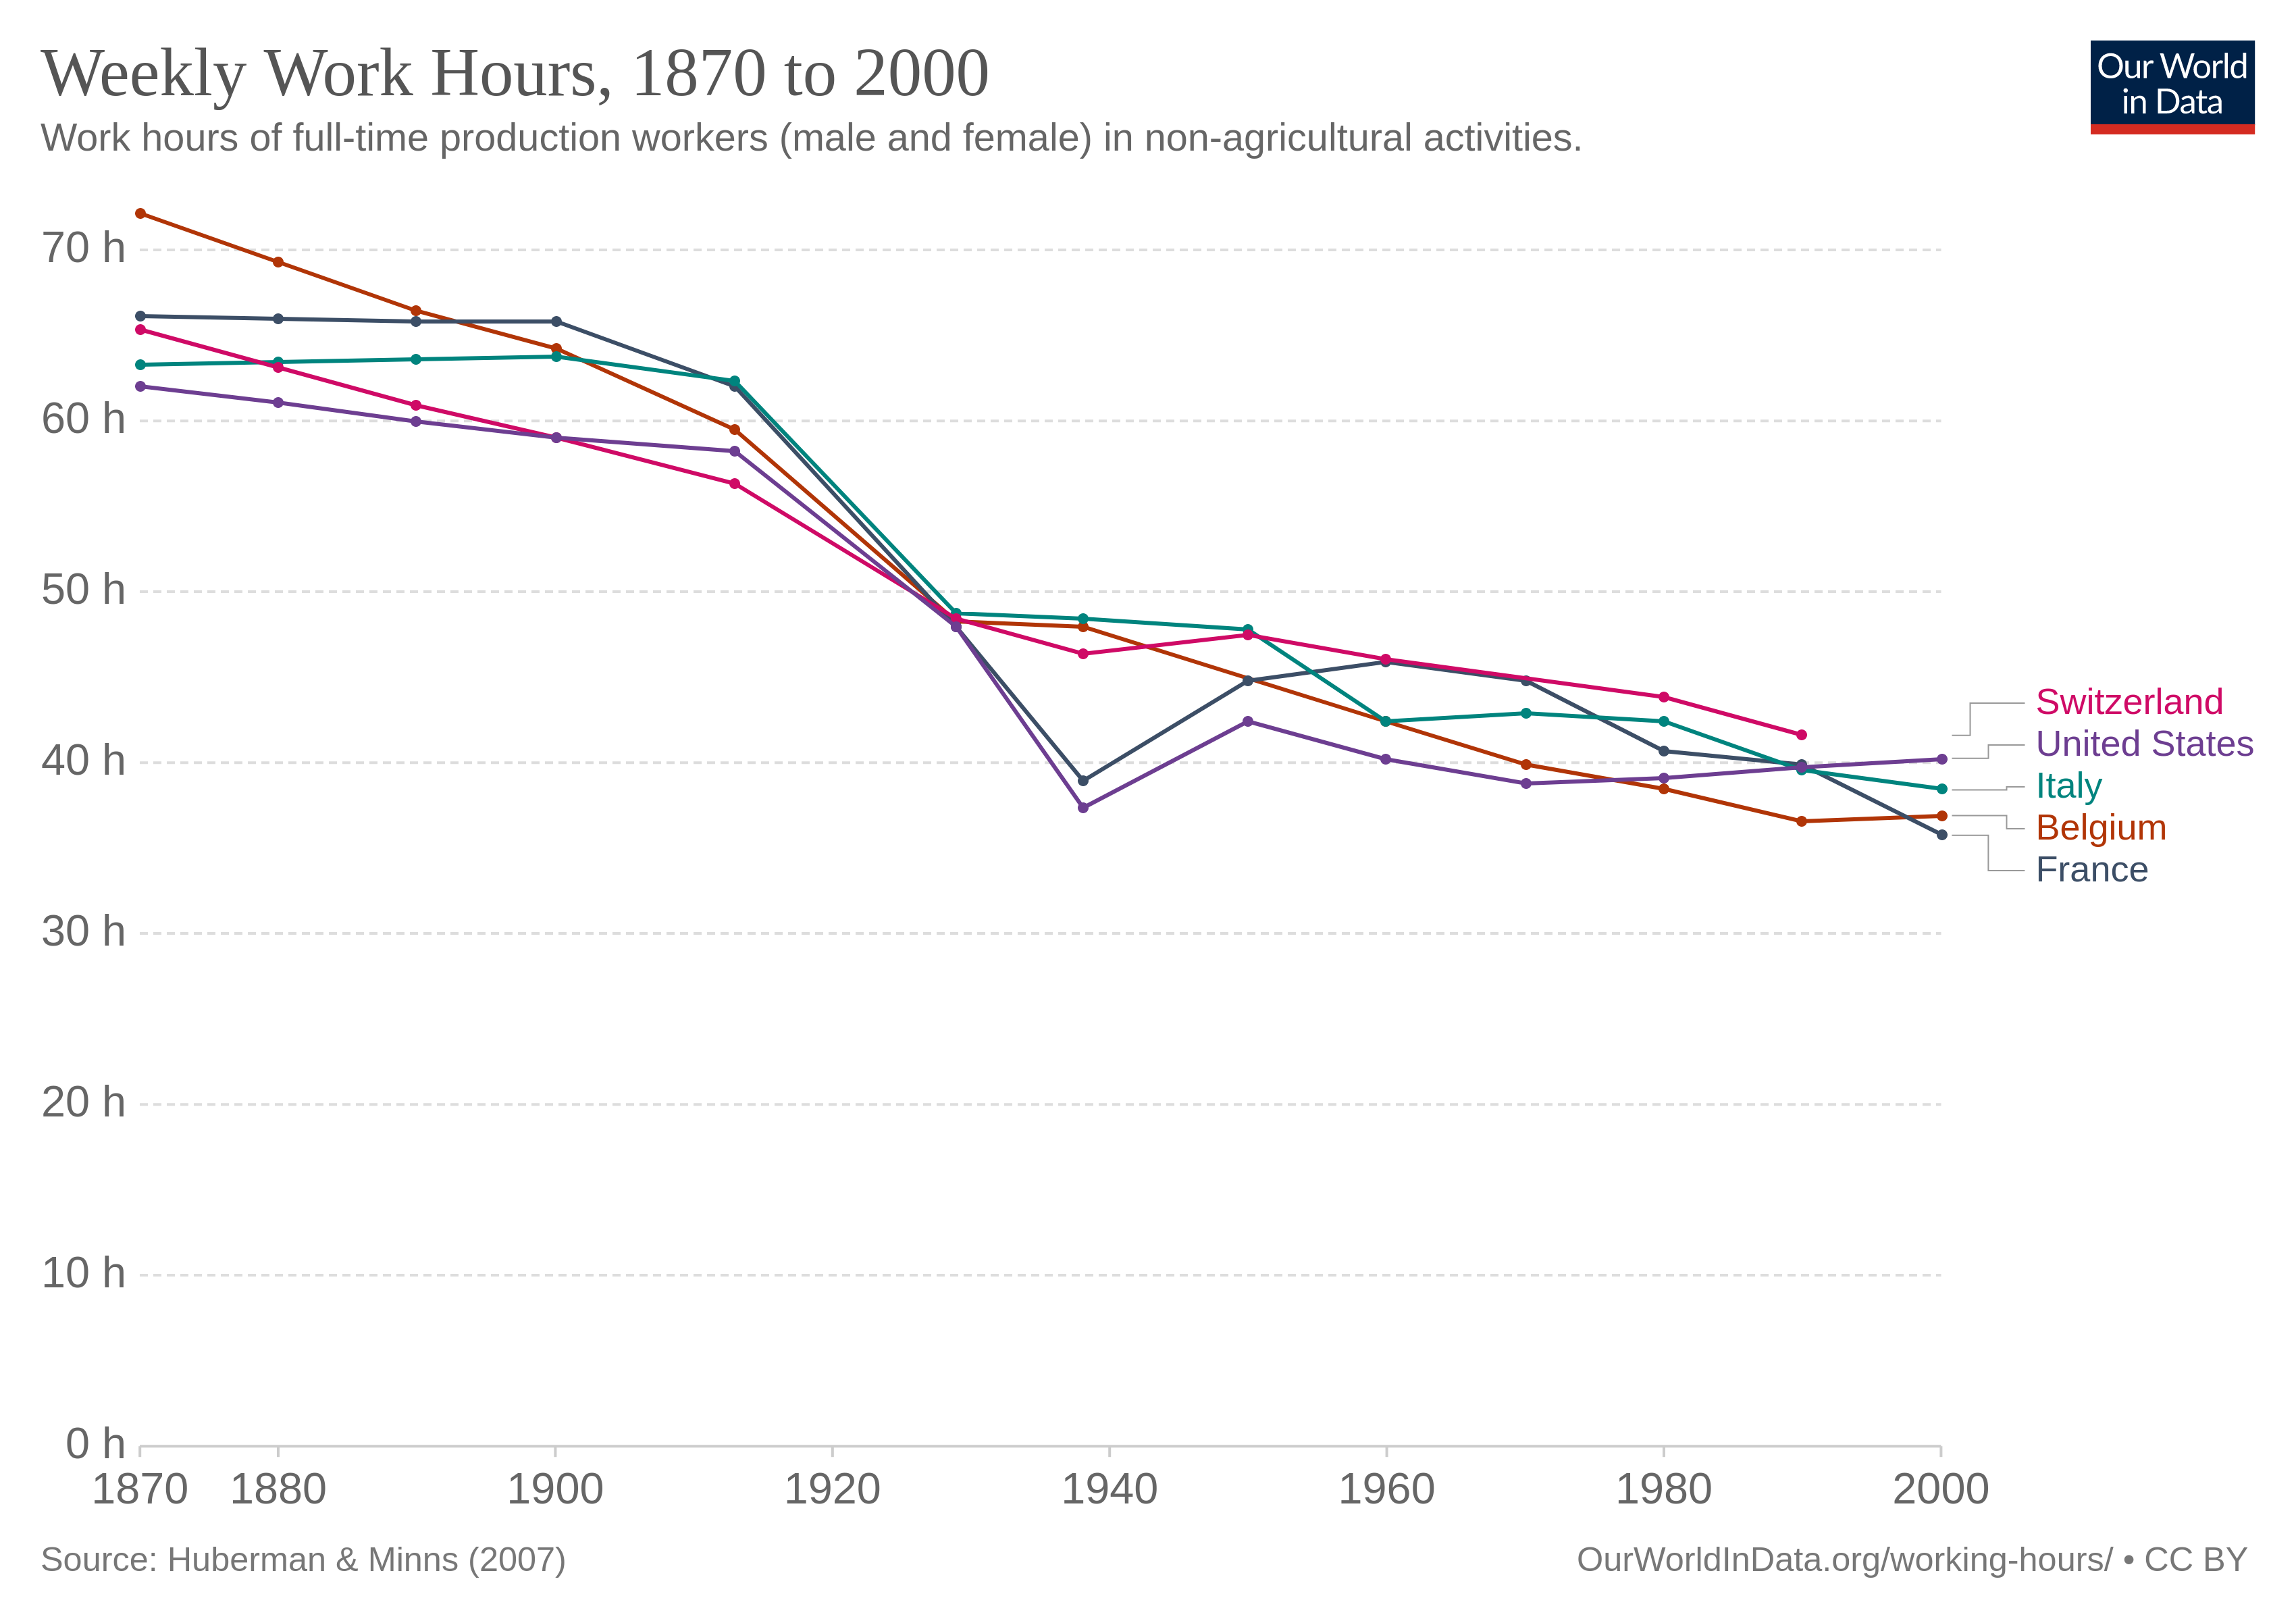
\includegraphics[width=0.8\linewidth]{images/Libro-img011.png}
    \caption{La settimana media di lavoro nel 1900 era di 60 ora mentre adesso è di 40 e, con condizioni e diritti
superiori grazie alle proteste e scioperi visti tra l'800 e il 900 e in seguito
negli anni 60 e 70
Credits: \raggedright\url{https://ourworldindata.org/grapher/work-hours-per-week?time=1870..2000\&country=BEL+FRA+ITA+CHE+USA}}
  \end{subfigure}
\end{tabular}
\end{table}

\begin{table}[H]
\centering
\begin{tabular}{cc}
  \begin{subfigure}{0.5\textwidth}
    \centering
    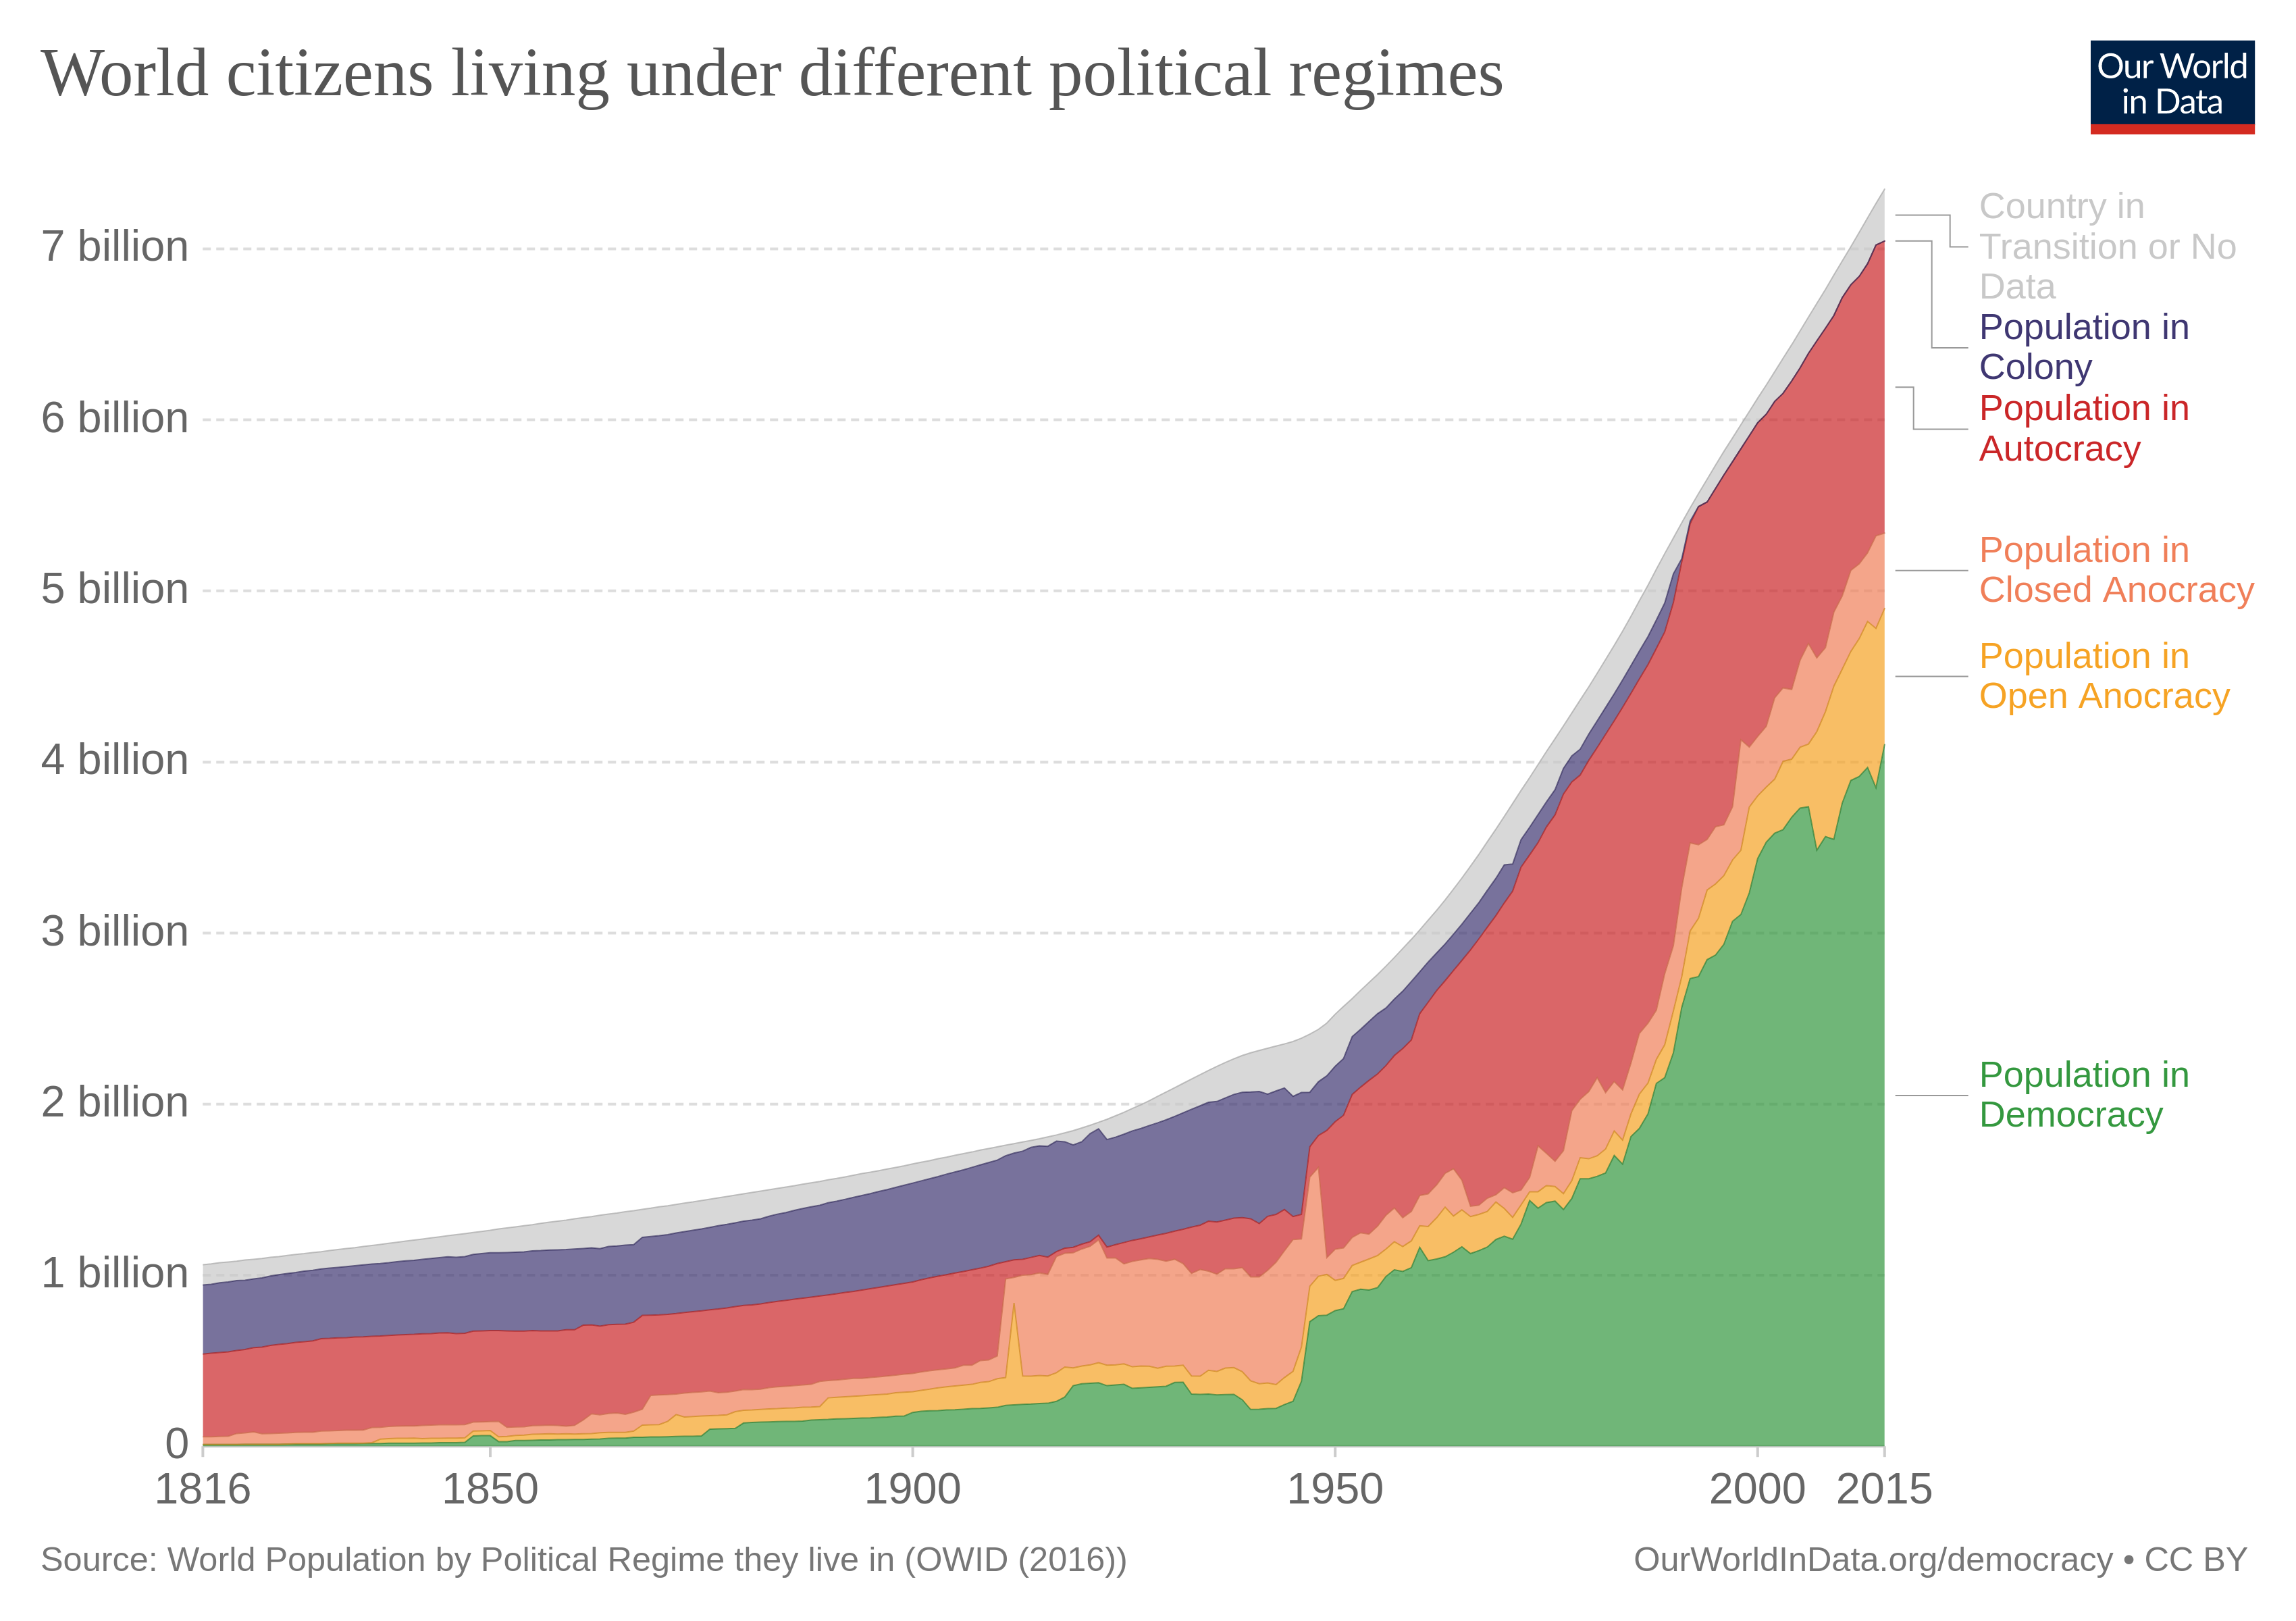
\includegraphics[width=0.8\linewidth]{images/Libro-img012.png}
    \caption{Sempre più persone vivono in governi democratici
Credits: \raggedright\url{https://ourworldindata.org/grapher/world-pop-by-political-regime}}
  \end{subfigure}
  &
  \begin{subfigure}{0.5\textwidth}
    \centering
    \caption{}
  \end{subfigure}
  \\
\end{tabular}
\end{table}

Secondo diversi indicatori raccolti da fonti come Our World in Data, negli ultimi decenni si è osservata una riduzione delle vittime di guerra e atti terroristici su scala globale, e un incremento nella produzione culturale e scientifica. Tuttavia, tendenze come la democrazia e i diritti umani mostrano variazioni significative tra regioni e periodi. Potete trovare numerosi altri indici su
ourworldindata.org. E altri grafici interessanti su:

www.gapminder.org/tools

www.gapminder.org/data

Mentre un'altra risorsa interessante è:
https://books.google.com/ngrams
Ad esempio, cercando il termine ‘omicidio’ su Google Ngram si osserva un aumento della sua frequenza nei testi pubblicati, anche se in molti paesi il tasso reale di omicidi è in calo da anni. Questo suggerisce una potenziale discrepanza tra percezione pubblica e dati oggettivi, anche se le cause di questa discrepanza vanno interpretate con cautela in quanto può essere dovuto anche ad altri fattori (fiction, dibattiti politici, ecc...).

Contrariamente alle aspettative comuni, nonostante le paure moderne, anche la propensione ad aiutare gli sconosciuti è in realtà aumentata negli ultimi cinquant’anni\endnote{\raggedright\url{https://www.eurekalert.org/news-releases/958742}}. Questo fenomeno, potrebbe essere influenzato da altri fattori positivi come l’incremento dell’istruzione, del reddito e  dell’urbanizzazione.

Con questo non intendo negare l'esistenza di problemi, ma sottolineare l'importanza di evitare di trasformare le singole criticità in generalizzazioni assolute e totalizzanti. Seppur ci siano ancora molte sfide da affrontare, è significativo riconoscere che, in diversi ambiti, la tendenza evidenzi un progresso.

\begin{mdframed}[linewidth=1pt]
Fake news e complotti

Anche le cose più semplici, andando a un livello di dettaglio maggiore, sono molto complicate da spiegare o
contro-intuitive, ovvero fenomeni che la logica, anche ragionevole, spiegherebbe in un modo, ma la realtà dimostra essere sbagliato. Ad esempio risulta intuitivo dire che è il sole che si muove attorno alla terra, ma sappiamo non essere così. 
Senza conoscenze di base in astronomia e fisica, può risultare difficile smentire certe teorie complottiste.
Quindi come posso scegliere qual è la versione giusta? 
Devo credere a qualcuno che lo sa verificare con i telescopi, o credere a qualcuno che è andato sullo
spazio o, credere a qualcuno che scrive un post sui social? In qualunque caso mi dovrò fidare di qualcuno. Per questo,
credere per credere, conviene farlo per qualcosa dove non è un singolo a dire qualcosa, ma un gruppo di esperti che
ottengono gli stessi risultati da un esperimento (peer review). Non possiamo solo affidarci alle nostre sensazioni o ai
nostri sensi. Solo con lo sguardo sarebbe difficile dire che siamo noi a girare attorno al sole. Le fake news e le teorie del complotto offrono risposte semplici e immediate a problemi complessi, spesso evitando il percorso più faticoso ma necessario di acquisire basi di pensiero critico e alfabetizzazione scientifica. Inoltre bisogna raccogliere
documentazioni, testimonianze, analisi, per demolire una teoria del complotto, o verificare le fonti. 
Mentre per creare una fake news basta un intuizione o un po' di fantasia.

\needspace{4cm}
\begin{figure}[H]
  \centering
  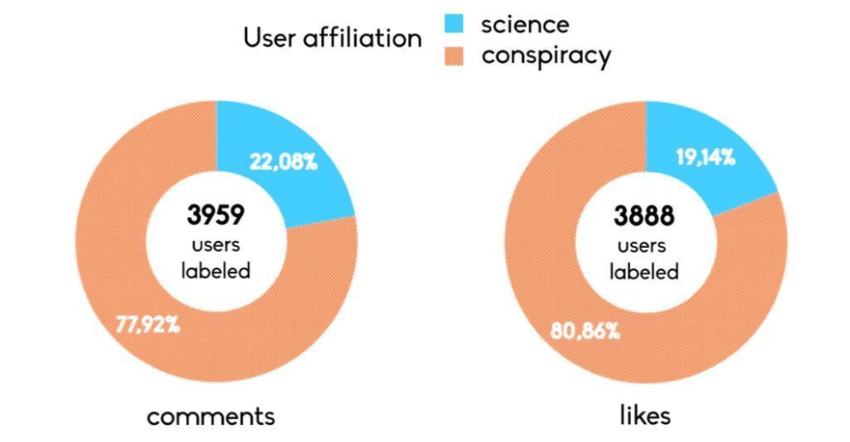
\includegraphics[width=0.95\linewidth]{images/Libro-img013.png}
  \caption{Credits: ResearchGate \raggedright\url{https://www.researchgate.net/figure/interaction-of-polarized-users-with-deliberately-false-information-Trolls-posts-We\_fig6\_33193629}}
\end{figure}

L'analisi riassunta da quest'immagine rappresenta che i post deliberatamente
falsi, fatti per divertimento da troll o semplicemente per ricevere più click e, di conseguenza più guadagni, ricevono
più like e commenti dai complottisti che, paradossalmente, nella ricerca della verità, possono rimanere aggrovigliati in questa
rete di notizie false.

È giusto sottolineare che complotto non significa necessariamente falso. Non possiamo dire cosa sia vero e cosa no in ogni contesto, ma
cosa abbia seguito un processo di analisi scientifico. Se non è scienza è
qualcos'altro, come pseudoscienza, che magari è pure vero e, se così fosse, un giorno forse si riuscirà a dimostrarlo. 
La questione riguarda solo il metodo che vogliamo adottare per indagare la realtà, alla luce di quanto la
nostra mente possa produrre distorsioni e, fin ora, il metodo più solido che l'umanità abbia
prodotto è proprio quello scientifico, per le ragioni viste precedentemente.

Quindi una domanda potrebbe essere: perché i complottisti non pubblicano su riviste scientifiche? Se hanno così a cuore
la divulgazione delle proprie scoperte? Come abbiamo visto prima, per via dell'anonimato sulle
revisioni, la scusa della censura da parte dei poteri forti può risultare così, per alcuni, una spiegazione debole. 


David Grimes ha proposto un metodo statistico per studiare i
complotti\endnote{\raggedright\url{http://journals.plos.org/plosone/article?id=10.1371/journal.pone.0147905}}. Grimes fonda la sua
teoria su una semplice idea: meno persone sono a conoscenza del complotto, più tempo rimarrà segreto.
Analizzando i dati del passato relativi ai complotti che sono stati scoperti, è riuscito a creare un modello matematico
in grado di stimare per quanto tempo un informazione può rimanere segreta in relazione al numero di persone coinvolte,
quindi calcolare la probabilità che ci sia una talpa o la possibilità di fughe di notizie.
Un complotto può restare segreto per 5 anni se ci sono meno di 2521 persone a conoscenza e, 100 anni se i cospiratori
sono meno di 125.
Questa scoperta rende improbabili molte teorie del complotto tra cui il mancato sbarco sulla Luna, cospirazione sui vaccini e l'esistenza di una cura segreta per il cancro.
Anche grandi aziende farmaceutiche (Bad Pharma di Ben
Goldacre\endnote{\raggedright\url{https://www.amazon.co.uk/dp/0007350740}}) o
l'NSA (National Security Agency) non sono riuscite ad eludere questa regola, famoso il caso di Edward
Snowden che denunciò lo stato americano di spiare i cittadini tramite siti come wikileaks.org o arxiv.org dove
possibile pubblicare fughe di notizie.

Riguardo al paranormale, James Randi nel 1996 fondò la James Randi Educational Foundation\endnote{\raggedright\url{https://web.randi.org}} che studia le
affermazioni riguardanti questi fenomeni. La fondazione mette in palio un premio di un milione di dollari per chiunque
possa dimostrare una capacità paranormale in un ambiente controllato (quindi i video non sono ammessi visto la possibilità di essere manipolati). 
Nessuno però è mai riuscito a superare il test preliminare, che viene
stabilito e concordato tra Randi e il candidato. Ad oggi nessuno è ancora riuscito a dimostrare un fenomeno paranormale.
Anche il CICAP opera nello stesso campo e ha stilato una serie di
requisiti\endnote{\raggedright\url{https://www.cicap.org/n/articolo.php?id=273076} } alla ricerca di verificare fenomeni paranormali.
\end{mdframed}


\begin{mdframed}[linewidth=1pt]
Ricerca scientifica non equivale a verità

Sul web e più in generale nel dibattito pubblico sembra essere nata, in alcune bolle, una battaglia tra i sessi. Quelli che dicono che indubbiamente e in ogni circostanza sono più svantaggiati i maschi e chi le femmine, portando dati a favore della propria posizione.
È importante riconoscere che entrambi i sessi affrontano difficoltà significative, ma spesso diverse per natura, visibilità e contesto. L'obiettivo non è sminuire il dolore di nessuno, ma evidenziare come una lettura semplicistica dei dati possa rafforzare polarizzazioni invece di contribuire alla comprensione.
Quello che vorrei fare, più che parlare di questi temi, è usarli come pretesto per mostrare come anche informazioni vere possano essere interpretate e non coincidano necessariamente sempre con una rigida verità. Gli esempi che porterò di seguito sono veri e contemporaneamente contrastanti tra loro. 
Se partiamo dalla fisica che studia i fenomeni del mondo possiamo fondare la chimica che si specializza sulla materia, su cui può sorgere la biologia crea medicinali oltre a studiare gli organismi, per arrivare alla medicina che grazie ai farmaci e non solo può curare gli esseri umani, che necessitano anche di aiuti mentali, grazie alla psicologia i cui effetti dipendono dall'ambiente che la sociologia cerca di conoscere. Più ci allontaniamo dalla fisica e più ci avviniamo all'essere umano prima nelle sue parti biologiche e poi nelle sue parti più astratte mentali fino ad arrivare ai gruppi di persone. Man mano che ci avviciniamo alla sociologia o ancora di più all'antropologia le variabili aumentano esponenzialmente e diventa sempre più difficile trovare una correlazione certa tra causa ed effetto, non potendo avere la sicurezza di aver compreso tutte le variabili. 
In questi esempi si mostrano le argomentazioni a vantaggio di uomini e donne seguite dalle variabili trascurate che rimettono in prospettiva questi argomenti.

Gli esempi che seguono non vogliono suggerire che i problemi degli uomini siano "più gravi" di quelli delle donne, o viceversa. Ogni dato va interpretato con attenzione, consapevoli del fatto che i vissuti individuali non si esauriscono nei numeri. Questo confronto osserva quanto sia difficile isolare la "verità" nei fenomeni complessi, soprattutto quando toccano identità, cultura e relazioni.

\begin{itemize}
\item Argomentazione maschile: Nel 2021 sul posto di lavoro sono morti 1.366 uomini contro 72 casi per le donne\endnote{\raggedright\url{https://www.inail.it/cs/internet/docs/alg-dati-inail-2021-giugno-luglio-pdf.pdf}} \endnote{\raggedright\url{https://nova.ilsole24ore.com/infodata/infortuni-sul-lavoro-1-200-morti-nel-2018-i-dati-settore-per-settore/}}.
Variabili trascurate: Statisticamente, gli uomini, grazie alla loro conformazione fisica possono fare lavori più fisicamente logoranti e pericolosi. 
\item Argomentazione maschile: I senzatetto maschi sono l'84\% e femmine 16\% le femmine\endnote{\raggedright\url{https://it.wikipedia.org/wiki/Senzatetto}}.
Variabili trascurate: gli uomini spesso finiscono per strada per dipendenze o problemi psichiatrici, che a loro volta possono dipendere dalla società e pressioni sugli uomini. Le donne più frequentemente per violenza domestica. Le donne possono sfuggire dalla condizione di senzatetto perché più facilmente trovano chi li ospita, altre finiscono nella prostituzione volontaria o meno, siccome per strada saranno più vulnerabili e non finiranno così in queste statistiche.
\item Argomentazione femminile: La violenza domestica è un fenomeno tragico che colpisce in modo grave migliaia di donne, uomini e bambini. Secondo Amnesty International una donna su tre ha subito violenza\endnote{\raggedright\url{https://www.amnesty.ch/it/news/2007/8-marzo-giornata-mondiale-della-donna}}. 
Variabili trascurate: Nella metà dei casi di coppia, la violenza è reciproca, mentre nell'altra metà il 70\% degli episodi di violenza è commessa dalle donne\endnote{\raggedright\url{https://ajph.aphapublications.org/doi/pdfplus/10.2105/AJPH.2005.079020}}. 
Variabili trascurate: Questo non significa negare la gravità della violenza contro le donne, né ignorare che le conseguenze fisiche e sociali siano spesso più pesanti per loro. Non tutte le violenze infatti sono infatti uguali, bisognerebbe distinguere tre le varie forme di violenza, verbale, fisica grave, minacce, clima di paura, controllo economico e, altre forme di conflitto. 
Variabili trascurate: conseguenze mediche. La violenza femminile, pur esistente, ha generalmente conseguenze meno gravi in termini di danni fisici, ricoveri o morti. 
Variabili trascurate: La vergogna sociale potrebbe portare gli uomini a denunciare meno l'aggressione della partner e così via all'infinito o quasi. Va aggiunto anche il timore sociale che spesso impedisce alle donne di lasciare una relazione violenta.
\item Argomentazione femminile: Nella violenza genitoriale i padri sono i principali responsabili della violenza sui figli.
Variabili trascurate: quasi il 40,0\% delle vittime è maltrattato da una madre che agisce da sola contro il 21,5\% che viene maltrattato da un padre che agisce da perché solo\endnote{\raggedright\url{https://www.acf.hhs.gov/sites/default/files/documents/cb/cm2018.pdf}}. Gli omicidi di bambini sotto l'anno di età sono compiute da donne nell'89,4\% dei casi\endnote{realizzata dall'Istituto di ricerche economico-sociali \raggedright\url{https://www.linkiesta.it/2019/09/maltrattamenti-minori-prevenzione-costi/}}).
Variabili trascurate: Le madri passano statisticamente più tempo con i figli, di conseguenza c'è una maggiore opportunità di conflitto, non si distingue tra diversi tipi di maltrattamento ecc...
Variabili trascurate: questo dato non distingue tra tipo di maltrattamento (psicologico, trascuratezza, abuso fisico grave).
\item Argomentazione maschile: In Italia gli stupri sono molto inferiori rispetto al resto d'Europa e del mondo\endnote{\raggedright\url{https://en.wikipedia.org/wiki/Rape_statistics}} \endnote{\raggedright\url{https://www.morewithdata.net/blog/20250108-Femicide-and-sexual-violence-in-Europe.html}} Regno unito con 117.3 vittime per 100.000 donne, Svezia 84.4, Francia 62.7, Nuova Zelanda 58.6, Islanda 45.4, Stati Uniti 41.4, Italia 12.41.
Variabili trascurate: Una donna potrebbe avere stigmi sociali che le impediscono di denunciare.
\item Argomentazione femminile: I femminicidi sono in aumento.
Variabili trascurate: Obiezioni su come vengono conteggiati:
\begin{itemize}
\item Donne trans
\item Suicidi: difficile provare il nesso con la violenza patriarcale
\item Movente: definizione di femminicidio.
\item Donne uccise da altre donne: difficile provare se il movente è legato a dinamiche patriarcali
\end{itemize}
Variabili trascurate: I dati che seguono non hanno lo scopo di minimizzare un fenomeno così grave come il femminicidio, ma di mostrare come i numeri, se isolati dal contesto, possano dare un’immagine incompleta o fuorviante. L’obiettivo è promuovere un’analisi più rigorosa, non una minimizzazione del problema.
In Italia nel 2020 ci sono stati 91 femminicidi, fenomeno che ha impattato per lo 0,00031\% (~29.5 milioni donne in Italia) nel 2022 sono stati 126, ovvero lo 0,00043\%. Quindi l'aumento dei femminicidi è stato del 38,46\% che sembra tantissimo, ma l'aumento del fenomeno nella sua totalità è del 0,00012\%. Su numeri così piccoli è difficile parlare di una tendenza o di cultura, infatti nel 2024 i femminicidi sono scesi a 113. Il fenomeno, seppur numericamente limitato, ha un forte impatto simbolico e richiede analisi approfondite: inoltre i dati non spiegano la sofferenza, ma servono a costruire risposte più efficaci.
Variabili trascurate: Il dato dei femminicidi nasconde inoltre un altro problema, quello degli omicidi che si potevano prevenire in quanto preceduti da denunce ignorate. I femminicidi sono tragedie che scuotono l’opinione pubblica e meritano attenzione, ma è importante affrontarli con rigore. I dati disponibili osservano che si tratta di eventi gravi ma numericamente limitati, spesso legati a dinamiche relazionali personali, non sempre prevenibili tramite interventi culturali generalizzati.
Non si può negare l’esistenza di relazioni tossiche, disfunzionali o violente, ma attribuire queste tragedie a un’intera cultura maschile, che condanna questi comportamenti, rischia di essere fuorviante. Allo stesso tempo, la società ha il dovere di continuare a impegnarsi nella prevenzione e nel supporto alle vittime, affinché nessuna persona debba vivere nella paura.
\item Argomentazione maschile: In Italia il divario salariale tra uomini e donne in Italia è tra i più bassi in Europa \endnote{\raggedright\url{https://ourworldindata.org/economic-inequality-by-gender}}.
Variabili trascurate: In Italia però la disoccupazione femminile è tra le più alte \endnote{\raggedright\url{https://en.wikipedia.org/wiki/Women\_in\_the\_workforce\#/media/File:Unemployment\_rate,\_women,\_OWID.svg}}.
Variabili trascurate: La disoccupazione dipende anche dalla prevalenza di donne in facoltà umanistiche di cui c'è meno richiesta
Variabili trascurate: La poca rappresentanza di donne nelle facoltà STEM (Scienza, Tecnologia, Ingegneria e Matematica) dipende da fattori culturali, a loro volta influenzati da altre variabili.
Parlare delle difficoltà che alcune donne incontrano nel lavoro non significa accusare gli uomini, ma riconoscere che ci sono ancora ostacoli, che limitano le scelte di tutti. Non sempre si tratta di colpa o di intenzione: fattori culturali, familiari o storici possono pesare sulle decisioni individuali. Affrontarli non è una battaglia tra sessi, ma un modo per permettere a ciascuno di esprimere davvero il proprio potenziale.
Il gender pay gap, è stato a lungo uno dei temi centrali delle battaglie per la parità. E con buone ragioni: in passato e ancora oggi, in molte situazioni le donne si trovano penalizzate da stereotipi, mansioni poco valorizzate o discriminazioni dirette e indirette.
\item Argomentazione femminile: Le donne ottengono generalmente voti più alti degli uomini durante il percorso scolastico e universitario. 
Variabili trascurate: alcuni studi\endnote{\raggedright\url{https://blueprintlabs.mit.edu/research/boys-lag-behind-how-teachers-gender-biases-affect-student-achievement/}} osservano che quando chi valuta non conosce il sesso dello studente, gli uomini tendono a ottenere punteggi più alti. Questo suggerisce che potrebbero esistere bias di genere impliciti nel processo valutativo.
Variabili trascurate: Le donne sono più vittime della sindrome dell’impostore, la minore autostima nelle materie STEM (che vedremo tra poco), ecc...
Riconoscere queste dinamiche non significa sminuire i successi delle ragazze, ma piuttosto promuovere un sistema educativo che valorizzi pienamente le diverse potenzialità di tutti.
\item Argomentazione maschile: Le donne guadagnano il 20\% in meno rispetto agli uomini.
Variabili trascurate: Numerosi calcoli sulla differenza di salario tra i generi vengono fatti semplicemente sommando gli stipendi di uomini e donne in percentuale, senza considerare: tipologia di lavoro (lavori STEM più remunerative e con prevalenza maschile), contratti (part time più diffuso tra le donne), Differenze regionali nel costo della vita ecc… con queste considerazioni la distanza si riduce ad un 5\%\endnote{\raggedright\url{https://www.pewresearch.org/short-reads/2025/03/04/gender-pay-gap-in-us-has-narrowed-slightly-over-2-decades}} \endnote{\raggedright\url{https://www.epi.org/publication/what-is-the-gender-pay-gap-and-is-it-real/}}. In altri indici, la differenza sembra arrivare anche a 0\endnote{An economist explains why women are paid less
\raggedright\url{https://www.weforum.org/agenda/2019/03/an-economist-explains-why-women-get-paid-less/}}.
Variabili trascurate: perché le donne scelgono più spesso il part-time? È davvero una scelta libera o è dovuta alla mancanza di servizi per l'infanzia e alla divisione diseguale del lavoro domestico?
Variabili trascurate: Le donne forse non scelgono materie STEM per condizionamenti sociali. Uno studio intitolato “draw scientists” chiedeva a dei bambini di disegnare uno scienziato. Il 99.4\% dei bambini e delle bambine disegnarono uno maschio, percentuale salita al 28\% nel 2018\endnote{\raggedright\url{https://srcd.onlinelibrary.wiley.com/doi/full/10.1111/cdev.13039}}.
Variabili trascurate: O forse gli uomini si sentono meno liberi di scegliere materie umanistiche che li arricchirebbero maggiormente come persone, sempre per lo stesso motivo, i condizionamenti sociali che richiedono all'uomo di prendersi cura della famiglia o che si sente in dovere di guadagnare più della donna.
Variabili trascurate: Secondo uno studio\endnote{\raggedright\url{https://papers.ssrn.com/sol3/papers.cfm?abstract_id=3048711}}, anche quando non si conosce il sesso dei partecipanti (nei lavori da remoto), le donne guadagnano comunque meno. Questo è un dato, ma non una sentenza. Potrebbe suggerire che non esiste una discriminazione a priori ma, nemmeno che le donne siano meno competenti. Le donne infatti, data la più frequente cura domestica, in remoto risultato più occupate e distratte, così da accettare lavori più semplici e meno retribuiti. Per questo paesi con politiche sociali di congedo parentale, che apparentemente avvantaggiano gli uomini, in realtà portano ad una disoccupazione femminile più bassa. Grazie a questa possibilità una donna orientata alla carriera, con un compagno più orientato alla famiglia, possono avere una vita più incline ai propri desideri. 
\end{itemize}

Quindi cercare di comprendere fenomeni complessi è una perdita di tempo, perché tanto non si riusciranno mai a contemplare tutte le variabili e le cause delle cause? No, è importante cercare di tentare di dare ordine al mondo per cercare di prevederlo, al meglio possibile trovato fino ad ora e fornire le migliori soluzioni, seppur non definitive o perfette.
Continuando a fornire nuove spiegazioni e trovando nuovi errori, pian piano, con cambiamenti purtroppo forse troppo lenti, si riuscirà ad avvicinarsi sempre di più a qualcosa che assomigli alla verità.
Questi esempi mi servono sono per dire che è importante continuare a informarsi, ma senza avere la certezza di aver trovato la verità definitiva, evitando di schierarsi in qualche gruppo. Quando ci schieriamo e ne facciamo parte della nostra identità, possiamo rischiare di arrivare a difendere quelle idee come noi stessi, portandoci ad assumere comportamenti esagerati e una rigidità mentale.
\end{mdframed}

\clearpage\section{Felicità}
\begin{mdframed}[linewidth=1pt]
Nota: Premetto che non sono uno psicologo e questo, quindi quello che segue deve essere preso in
quest'ottica. Io ho cercato di essere preciso con le note e i riferimenti ma ogni caso è a se, ad
esempio, se dovessimo trovarci davanti a una persona in crisi, potremmo essere portati a dare un consiglio ragionevole
come: fai dei bei respiri profondi e pensa a qualcosa di bello. Per alcune persone ansiose, questi consigli potrebbero
farli stare ancora peggio o provocare una fame d'aria che li farà sentire ancora più ansiosi.
In certi casi, offrire consigli non richiesti può essere percepito come invalidante e rischia di rinforzare un senso di inadeguatezza, soprattutto se non accompagnato da ascolto empatico. O ancora, se non si conosce il trauma e si va a scavare, il rischio è quello di far rivivere alcune esperienze e recare
un danno. Da non psicologo, preferisco ascoltare e non dare consigli non richiesti.
\end{mdframed}

\begin{mdframed}[linewidth=1pt]
Riassunto: Impariamo ad osservare i nostri pensieri, quando ci accorgiamo che stanno andando in una direzione che non ci è utile in questo momento, ritorniamo a ciò che stiamo facendo e alle nostre sensazioni fisiche, senza incolparci per non essere riusciti a rimanere concentrati. Anche perché questo sarebbe un altro pensiero inutile. Questo potrebbe essere un importante ingrediente della felicità: osserva ciò che c'è, non ciò che vorresti ci fosse. Una semplificazione può vedere una mente felice differire da una triste quando non sta etichettando o giudicando come infelice il suo mondo interiore. Noi non siamo i nostri pensieri. Non siamo tristi, stiamo provando tristezza, non siamo arrabbiati, stiamo provando rabbia. Accettare i pensieri negativi è parte del processo, senza cercare di reprimerli. Per questo è importante accorgersi dei giudizi e non alimentarli, cosa che spesso facciamo senza nemmeno rendercene conto.
Quando notiamo un pensiero che non ci serve in questo momento, mettiamolo da parte e dedichiamo un momento nella nostra giornata, anche 15 minuti, dove pensiamo solo a quello. Vietato pensare ad altro! In questo modo non sarà una fuga da noi stessi, ma un pensarci dopo, nel momento più opportuno, utilizzando anche la scrittura se vogliamo. Questo può essere utile per tornare a stare bene, ma se vogliamo fare qualcosa in più, iniziamo a sorridere e a guardare con meraviglia tutto ciò che solitamente diamo per scontato, a questo scopo è utile pensare, a fine giornata, a tre cose di cui siamo grati, anche cose piccole.
Giudicare non è il male, è importante fare valutazioni. Tuttavia, è utile imparare a sospendere il giudizio sui nostri pensieri interni, mentre è fondamentale mantenere un'attenta valutazione delle nostre azioni, assicurandoci che non causino danno ad altri.
Per fare questo serve attenzione. Da una parte ci permette di concentrarci sulle cose delle della vita, senza che ci passi davanti distrattamente e evitare la tendenza forse naturale a vedere principalmente i problemi. Allo stesso tempo ci permette di chiederci: perché faccio quello che faccio? perché per me è importante fare questo in questo momento? So ricostruire il processo decisionale che mi ha portato ad avere queste idee? Se non siamo consapevoli del processo che ha formato le nostre convinzioni, rischiamo di agire per abitudine o imitazione, piuttosto che secondo valori realmente riflettuti, non sto dando alla mia vita la forma che io reputo essere giusta per me, rischiando di non essere autentico.

Qualche esempio nella speranza di trovare quello giusto per te:
\begin{itemize}
    \item \textbf{Osservare i pensieri:} 
    \begin{itemize}
        \item \textbf{Situazione:} Stai lavorando e ti distrai pensando a un litigio avuto con un amico.
        \item \textbf{Azione:} Noti il pensiero e ti dici: "Questo non è il momento giusto per pensarci. Torno a lavorare e ne rifletterò alle 18."
    \end{itemize}

    \item \textbf{Gestire i pensieri inutili:} 
    \begin{itemize}
        \item \textbf{Situazione:} Ti senti in colpa per non essere riuscito a finire tutto quello che avevi programmato oggi.
        \item \textbf{Azione:} Scrivi su un quaderno: "Oggi non ho fatto tutto, ma ho comunque portato avanti X e Y. Domani mi concentrerò su Z."
    \end{itemize}

    \item \textbf{Non giudicare i pensieri:} 
    \begin{itemize}
        \item \textbf{Situazione:} Ti accorgi di pensare "Non sono abbastanza bravo in questo."
        \item \textbf{Azione:} Riconosci che è un giudizio e lo lasci andare, dicendoti: "È solo un pensiero, non definisce la mia realtà."
    \end{itemize}

    \item \textbf{Giudicare le azioni:} 
    \begin{itemize}
        \item \textbf{Situazione:} Hai passato troppo tempo sui social invece di studiare.
        \item \textbf{Azione:} Valuti il tuo comportamento e decidi di impostare un timer per limitare il tempo sui social il giorno dopo.
    \end{itemize}

    \item \textbf{Rimandare i pensieri:} 
    \begin{itemize}
        \item \textbf{Situazione:} Durante una passeggiata pensi a un problema finanziario.
        \item \textbf{Azione:} Ti dici: "Ne penserò dopo cena, ora mi concentro sul panorama e sul mio respiro."
    \end{itemize}
\end{itemize}

Troviamo un esempio: ripensa a quando è stata l'ultima volta che sei stato un po' triste? Come hai reagito?
\end{mdframed}

Il popolare corso di Yale sulla felicità intitolato “The Science of
Well-Being”\endnote{\raggedright\url{https://www.coursera.org/learn/the-science-of-well-being} } spiega già dai primi minuti, grazie
alla dottoressa Laurie Santos che avere un buon lavoro, guadagnare tanti soldi, trovare il compagno della vita, avere
un bel corpo, fama e status, non vi renderà felici. 
La felicità duratura difficilmente dipende solo dalla realizzazione di desideri o dall’approvazione esterna; questi fattori possono offrire soddisfazione temporanea, ma possono tendere a perdere effetto nel tempo.

La felicità dipende al 50 percento da fattori genetici\endnote{{}- Lyubomirsky, S. (2007). The How of Happiness: A New
Approach to Getting the Life You Want. Penguin books - Goldsmith, H. H. (1983). Genetic influences on personality from infancy to adulthood. Child Development, 54(2),
331–355. \raggedright\url{https://doi.org/10.2307/1129695}
{}- Nichols, R. C. (1978). Twin studies of ability, personality, and interests. Homo, 29, 158-173.}, al 10 dalle
circostanze della vita e al 40 da azioni, abitudini, intenzioni. La percezione che abbiamo è invece molto diversa,
probabilmente attribuiamo un 90\% ai fattori esterni. Anche eventi dolorosi, come la perdita di una persona cara, tendono a diminuire d’intensità nel tempo, grazie alla naturale capacità di adattamento dell’essere umano, anche se il processo può variare notevolmente da persona a persona. L'essere umano infatti ha una forte resilienza, ma in alcune situazioni, ci sforziamo di trattenere le emozioni, stati d'animo e pensieri auto sabotando e impedendo un
normale ritorno del benessere. Quindi, sebbene il 40\% attribuito alle nostre azioni e abitudini rappresenti l'ambito di intervento più diretto e consapevole, è importante riconoscere che anche gli altri fattori possono essere influenzati, seppur indirettamente, dalle nostre scelte e strategie. Se vogliamo
essere felici non possiamo sperare di avere il massimo fattore genetico e ambientale dalla nostra. Anche in presenza di condizioni ottimali, il nostro impegno attivo gioca un ruolo cruciale. In realtà, alcuni
studi\endnote{{}- Agnoletti, M. (2022). L'Epigenetica ed il Microbiota osservano quanto il
contributo genetico della Felicità sia stato finora largamente sovrastimato.
\raggedright\url{https://www.medicalive.it/il-contributo-genetico-della-felicita-agnoletti/} - Agnoletti, M. (2020). L'epigenetica e la sovrastima della componente genetica negli studi
gemellari \raggedright\url{https://www.medicalive.it/epigenetica-e-sovrastima-della-componente-genetica-negli-studi-gemellari/} - Agnoletti, M. (2021). La stima della componente genetica alla luce dell'Epigenetica e della
microbiota revolution
\raggedright\url{https://www.medicalive.it/la-stima-della-componente-genetica-alla-luce-dell-epigenetica-e-della-microbiota-revolution/} - Wong, A. H., Gottesman, I. I., Petronis, A. (2005). Phenotypic differences in genetically identical organisms: the
epigenetic perspective. Hum. Mol. Genet.,14, 11–18
\raggedright\url{https://academic.oup.com/hmg/article-abstract/14/suppl\_1/R11/560905}
{}- Fraga, M. F., Ballestar, E., Paz, M. F., Ropero, S., Setien, F., Ballestar, M. L., Heine-Suner, D., Cigudosa, J. C,
Urioste, M., Benitez, J., et al. (2005). Epigenetic differences arise during the lifetime of monozygotic twins. Proc
Natl Acad Sci U S A, 102, 10604–1069 \raggedright\url{https://www.pnas.org/doi/abs/10.1073/pnas.0500398102} - Yet, I., Tsai, P. C., Castillo-Fernandez, J. E., Carnero-Montoro, E., Bell, J. T. (2016). Genetic and environmental
impacts on DNA methylation levels in twins. Epigenomics, 8, 105–117.
\raggedright\url{https://www.futuremedicine.com/doi/abs/10.2217/epi.15.90}}, hanno messo in luce errori metodologi circa queste
ricerche in cui hanno trovato un valore del 50\% come fattore genetici della felicità. Sembra infatti che questo valore
sia sovrastimato, il che lascia spazio alla possibilità che comportamenti, abitudini e contesto abbiano un’influenza maggiore di quanto ritenuto in passato.

Possiamo misurare i nostri progressi grazie al test PERMA (acronimo di Positive emotions, Engagement, Relationships,
Meaning, Accomplishment) che potete trovare su permahsurvey.com 

\begin{mdframed}[linewidth=1pt]
Studi di felicità 

Alcuni studi suggeriscono che comportamenti come sorridere più spesso\endnote{\raggedright\url{https://www.eurekalert.org/pub\_releases/2011-02/msu-sfa022211.php}}, seguire una dieta ricca di verdure\endnote{\raggedright\url{http://journals.plos.org/plosone/article?id=10.1371/journal.pone.0171206}} e adottare condotte prosociali\endnote{\raggedright\url{http://journals.plos.org/plosone/article?id=10.1371/journal.pone.0051380}} possano contribuire, in misura variabile, a migliorare il benessere soggettivo. Il contatto fisico positivo, come gli abbracci, può aumentare il rilascio di ossitocina e favorire il benessere\endnote{\raggedright\url{http://www.ted.com/talks/paul_zak_trust_morality_and_oxytocin}}. Inoltre si raccomandano sette ore di
sonno e, mezz'ora di esercizio fisico al giorno per minimo tre volte la settimana, meglio se
all'aria aperta in quanto si tende a fare più pensieri positivi rispetto allo stare al
chiuso\endnote{Schertz, Kathryn E., et al. Environmental influences on affect and cognition: A study of
natural and commercial semi-public spaces. Journal of Environmental Psychology 83 (2022): 101852.
\raggedright\url{https://www.sciencedirect.com/science/article/abs/pii/S0272494422000974}}.

Un'indagine del Regno Unito condotta da Carrington nel 2016 osservò che tre quarti dei bambini
trascorrevano all'aperto meno tempo dei detenuti nelle carceri, mentre per il 20\% dei bambini era
normale non uscire neppure una volta in un'intera giornata! Credo che anche per gli adulti non si
otterrebbero risultati troppo diversi.

Spendere o risparmiare? I soldi fanno davvero la felicità? Uno studio di Kahneman e Deaton (2010) ha rilevato che, negli Stati Uniti, il benessere emotivo tende a stabilizzarsi oltre i 75.000 dollari annui. Tuttavia, ricerche più recenti osservano che il rapporto tra denaro e felicità è più complesso e può variare in base al contesto e alla personalità. Uno studio canadese ha suggerito che spendere per gli altri
garantisce una maggiore felicità che spendere la stessa cifra per sé. 
Per molte persone, i soldi possono contribuire alla felicità quando vengono utilizzati per acquisire più tempo libero, ad esempio delegando compiti come la cura del giardino o le pulizie, piuttosto che solo per l'acquisto di beni materiali. Anche il tempo da trascorrere da soli non va
trascurato, alcune ricerche suggeriscono che un certo intervallo di tempo trascorso in solitudine significativa, ad esempio tra le 2 e le 5 ore al giorno, potrebbe essere associato a livelli più elevati di benessere per alcune persone. Si ipotizza che questo tipo di solitudine sia distinto dal tempo trascorso in famiglia. I ricercatori hanno notato che con meno di 2 ore tendenzialmente è più difficile raggiungere un buon livello di benessere, ma con più di 5 ore non ci sono aumenti significativi\endnote{\raggedright\url{https://youtu.be/9j5m3EoFoe8} }
\endnote{\raggedright\url{https://www.huffpost.com/entry/free-time-happier\_l\_61422730e4b0ab42329f3d4e}
} \endnote{\raggedright\url{https://www.cnbc.com/2022/09/08/too-much-free-time-wont-make-you-happier-says-psychologist-how-many-hours-you-really-need-in-a-day.html}
} \endnote{\raggedright\url{https://www.psychologytoday.com/us/blog/psychology-money-and-happiness/202303/research-shows-how-much-free-time-you-need-to-be-happy}}.
Un sondaggio chiamato Rest Test, che ha coinvolto 18000 volontari in 135 paesi diversi, ha sottolineato come lo stare con gli altri non è arrivato nella top 10, è stato interpretato suggerendo che anche gli estroversi possono trovare riposo nella solitudine. Le attività considerate riposanti, inoltre, non sono state quelle meno faticose, ma quelle in solitaria, la classifica vede infatti: Lettura 58\%, stare nella natura 53,1\%, stare da soli 52,1\%, ascoltare musica 40,6\%, non fare nulla in particolare 40\%\endnote{\raggedright\url{https://www.sciencedaily.com/releases/2016/09/160928153541.htm}}. Va precisato che queste non sono necessariamente le attività che ci rendono più felici, ma solo più riposati.

Altri studi mettono in relazione il tempo trascorso all'aria aperta con un maggiore benessere psico-fisico. Chi vive in
città è più incline a sviluppare disturbi d'ansia e dell'umore, ma tendenzialmente ha un cervello che tollera meglio lo stress. Può
essere più soggetto a malattie polmonari, ma ha spesso a disposizione maggiori stimoli cognitivi, e più situazioni per
appagare la propria vita sociale. Alcuni studi suggeriscono che una socializzazione frequente, come quella quotidiana, possa essere associata a una maggiore longevità rispetto a una socializzazione meno assidua\endnote{\raggedright\url{https://www.focus.it/scienza/salute/vuoi-vivere-a-lungo-socializza-meglio-se-tutti-i-giorni}}.
Alcuni studi sul cosiddetto ‘blue space’ osservano che vivere vicino all’acqua, come coste o laghi, può essere associato a livelli maggiori di benessere psicologico, probabilmente per via dell’effetto calmante dell’ambiente naturale. Una ricerca inglese condotta su 15.000 persone in 14 diversi Stati europei ha osservato che coloro che hanno trascorso parte della loro infanzia o hanno vissuto lungo le coste marine o grandi laghi ottengono punteggi di benessere più alti da adulti\endnote{International survey - BlueHealth\raggedright\url{https://bluehealth2020.eu/projects/bluehealth-survey/}} \endnote{BlueHealth - University of Exeter\raggedright\url{https://bmjopen.bmj.com/content/7/6/e016188.abstract}}.

In un importante studio del 2018 pubblicato su The Lancet (Chekroud et al.,
2018)\endnote{\raggedright\url{https://www.sciencedirect.com/science/article/abs/pii/S221503661830227X}}, è stato chiesto a 1,2 milioni
di soggetti di compilare un questionario che mettesse in relazione attività fisica, reddito e disagio psicologico, come
ansia, stress o umore basso. I risultati hanno osservato che le persone fisicamente attive riportavano mediamente 1,49
giorni emotivamente negativi in meno ogni mese, quindi, 18 giorni di disagio in meno all'anno,
rispetto alle persone inattive ma più ricche. Quindi, più ci si allena e più si sta bene? No, troviamo anche in questo
fenomeno un andamento gaussiano, quindi se ci si allena troppo, o troppo poco, il benessere diminuisce. Il picco di
questa curva, ideale per il benessere mentale, è rappresentato da 3/5 giorni di allenamento a settimana di circa 45
minuti, allenarsi in eccesso (oltre le tre ore giornaliere), invece, è stato associato a livelli più bassi di benessere psicologico, rispetto a un’attività moderata. Tuttavia, questo effetto potrebbe dipendere anche da fattori come stress da prestazione o sovraccarico fisico\endnote{\raggedright\url{https://journals.plos.org/plosone/article?id=10.1371/journal.pone.0285041}}. 
Inoltre, i benefici maggiori tendono a vedersi in sport di gruppo.

Alcuni studi preliminari suggeriscono che le rughe e l’invecchiamento cutaneo possono influire anche su altri organi, rendendo importante mantenere la pelle sana non solo per motivi estetici, ma anche per la salute generale. Le creme antirughe e la biostimolazione, possono essere utili. In uno studio su volontari over 40, l’applicazione cutanea di rapamicina, un senomodulatore, ha ridotto i marcatori di senescenza cellulare. Un esperimento sui topi ha inoltre osservato che l’eliminazione delle cellule senescenti con un senolitico stimola la proliferazione delle cellule staminali nei follicoli piliferi, suggerendo un potenziale effetto ringiovanente. Tuttavia, serviranno ancora molti anni prima che tali sostanze possano essere usate in sicurezza\endnote{\raggedright\url{https://www.frontiersin.org/journals/physiology/articles/10.3389/fphys.2023.1297637/full}} \endnote{\raggedright\url{https://link.springer.com/article/10.1007/s11357-019-00113-y}} \endnote{\raggedright\url{https://www.nature.com/articles/d41591-024-00067-5}} \endnote{\raggedright\url{https://theglowmemo.com/retinol-and-vitamin-c}}.
\end{mdframed}

\needspace{4cm}
\begin{mdframed}[linewidth=1pt]
Felicità e social

\begin{wrapfigure}{i}{9cm}
  \centering
  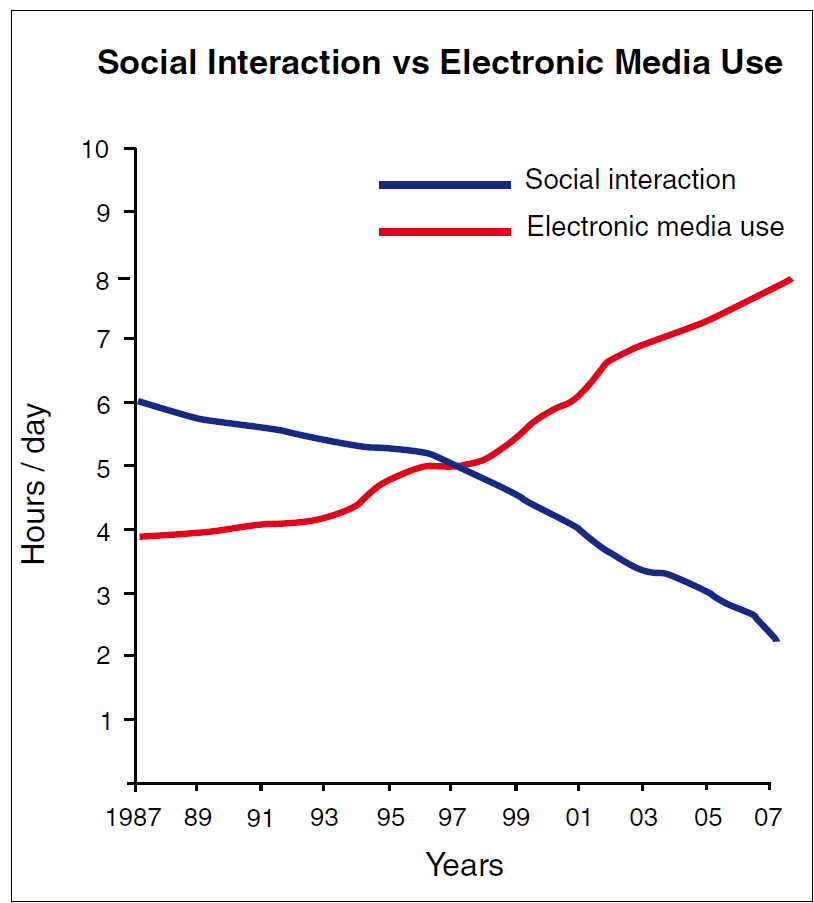
\includegraphics[width=0.95\linewidth]{images/Libro-img056.png}
  \caption{Analisi storica: le interazioni faccia a faccia sono diminuite, mentre sono aumentate quelle digitali (TV, radio, social media)\protect\endnote{Well connected? The biological implications of ‘social networking’ \raggedright\url{https://www.aricsigman.com/IMAGES/Sigman_lo.pdf}}}
\end{wrapfigure}

Chi usa i social network in modo attivo, ovvero pubblicando contenuti, può trarne benefici, anche se esiste il rischio di sviluppare comportamenti narcisistici. Al contrario, un uso passivo, cioè limitarsi a fruire dei contenuti altrui, è stato associato a una minore soddisfazione nella vita\endnote{Passive social network usage and life satisfaction among Vietnamese university students: a moderated mediation model of self-esteem and gender\raggedright\url{https://www.semanticscholar.org/paper/Passive-social-network-usage-and-life-satisfaction-Nguyen-Dang/7151b8ecc33af2a0b81e2244420be2f48937db75}}. Il problema è che ciò che viene condiviso online tende a rappresentare principalmente momenti eccezionali e positivi, creando una distorsione: si ha la falsa impressione che gli altri vivano costantemente esperienze straordinarie, mentre noi siamo fermi davanti a uno schermo.

Inoltre, i social costruiscono delle “para-relazioni” che possono illudere il cervello di avere una vita sociale appagante. Questo può ridurre la motivazione a impegnarsi in relazioni autentiche e offline, spesso più faticose da mantenere. Per chi sta attraversando un momento difficile, queste scorciatoie digitali, come community online, videogiochi o i social stessi, rischiano di diventare rifugi che impediscono di sviluppare strumenti per affrontare la realtà. Tuttavia, in altri casi, questi strumenti possono offrire supporto emotivo e senso di appartenenza. Alcuni studi suggeriscono che l’uso intensivo dei social media, soprattutto in modalità multitasking, potrebbe essere associato a una ridotta capacità di attenzione sostenuta. Tuttavia, le evidenze non sono ancora univoche. Quel che è certo è che il tempo dedicato ai social è tempo sottratto ad altre attività come lavorare, studiare o conversare. Se però l’uso resta contenuto, possono offrire anche momenti di svago e rilassamento.
La comunicazione ormai passa in gran parte attraverso gli smartphone. In un contesto altamente digitalizzato, un gruppo che scegliesse di rinunciare completamente ai dispositivi mobili potrebbe incontrare difficoltà a comunicare con il resto della società circa la sua rivoluzione.

Usare attivamente i social non ci rende comunque immuni ai problemi: Ogni volta che pensiamo di pubblicare qualcosa, difficilmente non penseremo all'effetto che potrebbe avere su chi lo guarderà, quale inquadratura usare, che testo scrivere ecc... così la nostra attenzione si allontana dal momento presente e si concentra sulla percezione che vogliamo generare negli altri. In questo modo, si rischia di vivere esperienze non per piacere personale, ma prevalentemente per mostrarci agli altri. Alcune attività potrebbero venire trascurate perché non “instagrammabili”. In certi casi, ciò può compromettere il valore esperienziale, attivando dinamiche mentali che finiscono ridurre la propria autenticità.

Il rischio è ancora più evidente negli adolescenti. Diversi studi hanno trovato una correlazione tra un uso molto prolungato dello smartphone (oltre 4 ore al giorno) e un aumento di sintomi psicologici negativi tra gli adolescenti, anche se non è chiaro se il tempo online sia causa o conseguenza di queste difficoltà. Alcuni studi suggeriscono che un uso moderato dei social (1–2 ore al giorno) possa essere associato a migliori indicatori di benessere rispetto a un uso nullo, probabilmente perché permette di mantenere contatti sociali e senso di appartenenza\endnote{\raggedright\url{https://www.focus.it/scienza/salute/adolescenti-e-smartphone-dopo-quanto-e-a-rischio-la-salute}}. Tuttavia, gli studiosi avvertono che non c’è una prova diretta di causalità: è possibile che siano proprio i giovani già vulnerabili a rifugiarsi più facilmente nei social.

Quindi i social fanno male? Dipende! Uno studio\endnote{The Impact of Using Mobile Social Network Applications on Students' Social-Life \raggedright\url{https://www.semanticscholar.org/paper/The-Impact-of-Using-Mobile-Social-Network-on-Abdelraheem-Ahmed/0868edadf30ebb8cac8a812a3deb27d3e8f65bde}} mostra che un uso moderato dei social può migliorare le relazioni sociali, familiari e la consapevolezza delle questioni attuali. Tuttavia, se l’uso è eccessivo, il benessere psicologico e le relazioni reali possono risentirne. Altri studi\endnote{Comparing the Happiness Effects of Real and On-Line Friends \raggedright\url{https://journals.plos.org/plosone/article?id=10.1371/journal.pone.0072754}} \endnote{3 Reasons Real-Life Social Support Is Best for Mental Health \raggedright\url{https://www.psychologytoday.com/us/blog/the-athletes-way/202105/3-reasons-real-life-social-support-is-best-mental-health}} suggeriscono che il numero di amici reali è correlato positivamente con il benessere soggettivo, mentre la dimensione delle reti online non ha effetti significativi.
Come ha osservato Matthias Mehl dell'Università dell'Arizona, non è solo il tempo passato
insieme a essere importante, ma come lo si passa. Osservando gruppi di adulti ha notato che è il tempo impiegato in
conversazioni significative con un'altra persona a essere correlato con la soddisfazione di vita, meno invece il tempo trascorso in chiacchiere superficiali. 
\end{mdframed}

Dagli anni 70 Nazioni Unite e Organizzazione per la cooperazione e lo sviluppo economico creano un rapporto sulla
felicità su worldhappiness.report ma uno studio pubblicato su Nature Human
Behaviour\endnote{\raggedright\url{https://www.nature.com/articles/s41562-019-0750-z}} ha sviluppato un modello per generare dati
precedenti agli anni 70 di Stati Uniti, Regno Unito, Germania e Italia, ma come? Analizzando libri e giornali raccolti
in Google Books, dal 1820 al 2009, un software tenendo conto dell'evoluzione del linguaggio ha
potuto analizzare l'umore percepito dell'epoca, quello che è emerso è che la
nostra resilienza del benessere soggettivo aumenta e diminuisce a seconda di cosa si sta vivendo, ma spesso temporaneamente. Una guerra tende a ridurre il benessere soggettivo, ma secondo alcuni modelli di adattamento, nel tempo molte persone tornano a livelli simili di felicità, anche se la velocità e la probabilità di questo recupero variano da individuo a individuo. Questo fenomeno si chiama habituation, può funzionare in grandi gruppi, come uno
stato, e anche per i singoli. In molte persone, anche dopo eventi traumatici come la perdita di una persona cara o un’invalidità, si osserva un progressivo adattamento, che può portare nel tempo a un recupero parziale o totale del benessere percepito. Stesso discorso vale anche
al contrario, l'aumento di salario potrebbe darci felicità per un periodo, ma poi si tende ad abituarcisi\endnote{\raggedright\url{https://www.focus.it/comportamento/economia/felicita-nazionale-livello-secoli-passati}}.

“La felicità è come una farfalla; più cerchi di inseguirla, più ti eluderà. Ma se sposti la tua attenzione su altre
cose, si siederà dolcemente sulla tua spalla.” - Henry David Thoreau.

Locke: "Non sono più sperduto." 
Sun:" E come ci sei riuscito?" 
Locke: "Nel modo in cui si ritrovano le cose perdute: ho smesso di cercare…
Tratto dalla Serie TV Lost Stagione 2 episodio 5 (Oggetti smarriti)

La parola felicità, in molte lingue, come l'inglese (happiness) ha una radice che significa
“accadere”, “per caso” (happen). Mentre solitamente le persone la ricercano e poi tentano di tenerla stretta, in questo
modo perde la sua eventualità e la relativa sorpresa, novità e meraviglia. Non è soltanto una questione linguistica,
paradossalmente, se noi volessimo cercare la felicità, tra le cose da fare c'è proprio lo smettere di cercare.
Esattamente come sforzarsi di essere spontanei: è un errore intrinsecamente logico. Una volta che iniziamo a cercare ce
lo aspettiamo, come un pacco regalo di cui sappiamo già il contenuto, non sarà più una sorpresa. Forse vi sarà
capitato di aver organizzato una serata con delle vecchie amicizie, dove avere riso e vi siete divertiti più che mai.
Così, organizzate nuovamente quella serata, ma vi accorgete che l'incantesimo si è spezzato. Vi
sareste aspettati che ricreando le stesse condizioni, la gioia si sarebbe ripresentata allo stesso modo e, invece, non
è successo. Abbiamo diverse esperienze di questo fenomeno, sarà capitato a tutti di aver difficoltà a dormire qualche volta e, di notare che il sonno difficilmente arriva con lo sforzo. E così anche la felicità. 
E così, spesso si osserva un effetto paradossale anche con la felicità: un tentativo eccessivo di calmarsi può aumentare l'ansia, un eccessivo sforzo di motivazione può ridurne la spontaneità, e una ricerca ossessiva della felicità può paradossalmente renderla più elusiva.
Se ti dico di non pensare a un elefante bianco, probabilmente ci penserai. Allo stesso modo, se ti ripeti di non provare ansia, paura o preoccupazioni, potresti finire per provarle. Abbiamo imparato erroneamente che bisogna fare l'opposto (scacciare le cose brutte con le cose belle) mentre invece può essere vincente imparare a utilizzare quella energia.
Cerchiamo di non essere schiavi della felicità.

Come scritto in "Pensaci ancora"\endnote{\raggedright\url{https://www.amazon.it/dp/8823838312}}, più le persone danno valore alla felicità, ed è meno probabile che riescano a vivere una vita felice\endnote{Iris B. Mauss et al., «Can Seeking Happiness Make People Unhappy? Paradoxical Effects of Valuing Happiness», Emotion, 11, 2011, pp. 807-815}. Questo fenomeno interessa sia chi è naturalmente incline a cercare la felicità, sia chi viene invitato a riflettere sull'importanza di essere felice. Esistono anche evidenze che attribuire troppa importanza alla felicità possa aumentare il rischio di depressione\endnote{Brett Q. Ford et al., «Desperately Seeking Happiness: Valuing Happiness Is Associated with Symptoms and Diagnosis of Depression», Journal of Social and Clinical Psychology, 33, 2014, pp. 890-905}. Una spiegazione potrebbe essere che, nella ricerca costante della felicità, siamo così intenti a valutare la nostra vita da non riuscire a viverla autenticamente. Anziché godere dei momenti di gioia, ci troviamo a riflettere su cosa ci manchi per essere ancora più felici. Inoltre, un’altra possibile ragione è che trascorriamo troppo tempo a inseguire il massimo livello di felicità, dimenticando che questa dipende più dalla frequenza delle emozioni positive che dalla loro intensità\endnote{Ed Diener, Ed Sandvik, William Pavot, «Happiness Is the Frequency, Not the Intensity, of Positive versus Negative Affect», in Fritz Strack, Michael Argyle, Norbert Schwartz (eds), Subjective Well-Being: An Interdisciplinary Perspective, New York, Pergamon, 1991}.

«Sono felici solo le persone che hanno la mente fissa su qualche oggetto diverso dalla propria felicità; sulla felicità degli altri, sul progresso dell’umanità o su qualche forma di arte o di ricerca, perseguita non come un mezzo, ma come un fine ideale. Mirando a qualcos’altro, finiscono per trovare la felicità» - John Stuart Mill

In uno studio\endnote{\raggedright\url{https://psycnet.apa.org/doiLanding?doi=10.1037\%2Fa0022010} } i partecipanti sono stati divisi in
due gruppi. In uno si faceva leggere un falso articolo che illustrava i vantaggi della felicità.
L'altro gruppo, quello di controllo, invece leggeva un articolo che non faceva riferimento alla
felicità. In seguito, entrambi i gruppi hanno guardato dei videoclip che avevano per argomento la felicità o la
tristezza. I partecipanti che hanno letto l'articolo che dava valore alla felicità si sentivano
meno felici rispetto al gruppo di controllo che aveva guardato lo stesso video. Dare troppo valore alla felicità ha
aumentato le loro aspettative riguardo al modo in cui le cose “sarebbero dovute essere” e, quindi, li ha predisposti
alla delusione. Un altro
studio\endnote{\raggedright\url{https://www.researchgate.net/profile/Jonathan-Schooler/publication/303158395\_The\_explicit\_pursuit\_and\_assessment\_of\_happiness\_can\_be\_self-defeating\_study\_1/links/58b480a692851cf7ae941179/The-explicit-pursuit-and-assessment-of-happiness-can-be-self-defeating-study-1.pdf}
}, è giunto alla stessa conclusione. I partecipanti hanno ascoltato una canzone disarmonica: La saga della primavera di
Stravinsky. Ad un gruppo è stato chiesto di "provare a sentirsi quanto più possibile
felici" durante l'ascolto. Successivamente, sono stati valutati e
riconosciuti come meno felici rispetto al gruppo di controllo che non stava inseguendo lo uno stato
d'animo felice. 

Abbiamo risultati che osservano come sfogare la rabbia raramente aiuta a liberarcene e, che nei report dei paesi più felici i manuali di self help non hanno più successo,
né la psicoterapia è più diffusa. Quindi forse la ricerca della felicità non aiuta a rendere più felici, anzi, forse il
contrario. Alcuni studi osservano che dare troppa importanza alla felicità può paradossalmente ridurre la percezione di benessere, specialmente se si creano aspettative irrealistiche o si tende a valutare costantemente il proprio stato emotivo. 

Chiediti se sei felice e cesserai di esserlo - John Stuart Mill.

\subsection{Come funziona la nostra mente?}
Questa è una domanda a cui probabilmente nessuno sa rispondere in assoluto, ma forse, relativamente al benessere ne sappiamo già
abbastanza. Anzi, la cosa strana è come mai se ne parli così poco nonostante certe cose si conoscano da sempre! Alcuni concetti espressi da filosofi antichi, come quelli dello stoicismo o del buddismo, risultano sorprendentemente coerenti con aspetti del benessere psicologico indagati oggi dalla scienza.

“Ciò che turba gli uomini non sono le cose, ma le opinioni che essi hanno delle cose”. Epitteto.

Il nostro benessere è strettamente correlato ai giudizi e alle aspettative, che sono una forma di giudizio. Noi siamo
turbati quando abbiamo aspettative sul mondo, il futuro, le persone, ma anche giudizi sui nostri pensieri, in quanto molto spesso crediamo di essere i nostri pensieri.

Il compito del cervello non è quello di generare verità, su di noi o sul mondo, ma quello di fare ipotesi e contro
ipotesi. Il nostro cervello pensa a tutto e pure al suo contrario, per questo motivo fatica a dire chi siamo senza ripensamenti. Ma perché
è così contraddittorio? Il nostro organismo è costruito per farci sopravvivere, e il cervello, attingendo dal
passato prova a creare ipotetici scenari sul presente e sul futuro nel tentativo di farci trovare pronti anche alle
eventualità più remote e improbabili. Non dovremmo preoccuparci se la nostra mente è insicura. Ci
dovremmo preoccupare se mostrassimo una totale assenza di dubbi (vedi bias cognitivi).

Facciamo un gioco, ora ti chiederò di fare una cosa, sei pronto?

NON pensare a un elefante bianco. 

Cos'è successo? Scommetto che nella tua immaginazione è appena apparso un bellissimo elefante
bianco! Ma perché? Eppure ti è stato chiesto di non fare proprio quello, avresti potuto fare altro e pensare a
qualsiasi altra cosa ma non quello! Come dicevamo, il compito del cervello non è fare quello che gli diciamo, non è
quello di dire la verità su cosa sentiamo su di noi, gli altri o le cose in generale, non è quello di dirci cose carine
o motivarci, ma semplicemente simulare ipotesi e il loro contrario. Se crediamo di essere delle cattive persone, la
nostra mente che può generare di tutto e, anche il suo contrario, saprà trovare episodi in cui siamo stati cattivi, o
potrebbe reinterpretarli alcuni neutri, ma in una luce negativa. Se ci convincessimo che siamo cattivi la nostra
mente potrebbe iniziare a dirci: No, non è vero, in questi episodi sei stato bravo! In altri casi invece la nostra mente tenderà a selezionare ricordi e interpretazioni coerenti con quella visione, rinforzandola. Se cerchiamo qualche pensiero,
molto probabilmente lo troveremo (rebound effect) e possiamo fare anche il contrario. Per questo frasi come “dai… Cerca di
non pensarci!” difficilmente potranno funzionare. Non possiamo non pensare, ma pensare ad altro. Quando ci accorgiamo di un pensiero
possiamo ritornare su quello che stavamo facendo, con gentilezza, senza punirci per aver fatto quel pensiero. È un
po' come fare qualcosa mentre si ascolta la radio, se ci sforziamo di non ascoltarla, succede
proprio l'opposto. Mentre se ci concentriamo sul nostro compito senza sforzarci di non ascoltare
la radio, quest'ultima diventerà un suono di sottofondo.

Quando cerchiamo di non pensare a qualcosa, come un elefante bianco, la nostra mente periodicamente dovrà chiedersi:
come sta andando il mio tentativo di non pensare a un elefante bianco? E in quel esatto istante dovrà per forza
rievocare questa immagine. Una tecnica nota come “intenzione paradossale” aiuta in questo, in quanto intenzionalmente
portiamo attenzione al pensiero che stiamo cercando di evitare. In alternativa siccome non possiamo non pensare,
possiamo però pensare ad altro e, portare l'attenzione su ciò che stavamo facendo. 

Ma se sono troppo indulgente con me, ricadrò sempre negli stessi pensieri negativi! 

Se siamo troppo severi con noi stessi, le probabilità che in futuro ci potremmo accorgere nuovamente di
questi pensieri, diminuiscono, perché il nostro cervello potrebbe ammonire qualcosa che ci fa stare male. 

Ma allora il giudizio, anche quello sui nostri pensieri è sempre negativo?

No, il giudizio è fondamentale per prendere decisioni. Il problema è quando lo facciamo inconsapevolmente, senza
l'aver scelto consapevolmente di indirizzare la nostra attenzione e i nostri giudizi verso la
risoluzione di un problema. Giudicare i nostri pensieri può diventare disfunzionale come abbiamo visto, per la natura stessa del
cervello. Mentre giudicare le nostre azioni invece è molto proficuo. Noi non siamo i nostri pensieri ma anche e significativamente con le nostre azioni. Aristotele diceva che siamo quello che facciamo ripetutamente, non ciò che diciamo di essere. Anche qua però, anche se ci accorgiamo di non aver agito come avremmo voluto, non dobbiamo metterci in croce, perché altrimenti le probabilità che commetteremo nuovamente quell'errore aumenteranno. 

Ma quindi chi siamo? Il nostro corpo è un accumulo di cibo, può essere tuo ma non può essere te. I tuoi pensieri sono un
accumulo di cose che hai visto, cose che ti hanno detto, ragionamenti, quindi possono essere tuoi ma non possono essere
te. Alcuni filosofi hanno detto che noi siamo le nostre azioni, Quindi chi siamo\endnote{“Conosci te stesso” può
diventare un ossessione \raggedright\url{https://www.youtube.com/watch?v=V61SSJL-gLo} }? Qual è il senso della vita? Queste sono domande
potenzialmente pericolose perché probabilmente non troveranno una risposta certa e si potrebbe finire in una spirale infinita. Tuttavia, se esplorate con consapevolezza e supporto, possono anche promuovere una maggiore autenticità e crescita personale. Cerchiamo quindi di non tenerle troppo nella nostra testa, possiamo scrivere o parlarne con qualcuno per non rischiare di rimanere intrappolati. Quando pensi, pensi a tutto e al contrario di tutto, mentre quando si scrive, si prendono piccole decisioni. Scrivere domande esistenziali può aiutare a chiarire pensieri e stati d’animo. Tuttavia, in alcune situazioni, se usata come forma di ruminazione senza guida o per lenire dei dolori, può generare ulteriore confusione o angoscia. 
Secondo Gennaro Romagnoli la maggioranza delle persone che vanno in analisi da uno psicologo è perché si fanno domande irrisolvibili come queste.

Un esercizio interessante potrebbe essere quello di
chiedersi: sono i miei vestiti? Sono i miei figli? Sono il mio corpo? Sono i miei pensieri? Sono la mia casa? Ci
accorgeremo che è impossibile trovare il nostro io fisso e immutabile. Il nostro io ci accade. A volte ci accorgiamo di aver reagito ad un
certo avvenimento in maniera inaspettata da quello che avremmo pensato, positivamente o negativamente; è capitato a
tutti. L'io è il rapporto tra la nostra genetica, la nostra storia e, il momento attuale. Possiamo
essere testimoni del nostro io e vedere come sta accadendo, come si sta manifestando. Questo ragionamento non serve a
deresponsabilizzarci e giustificare le nostre azioni come se compiute da un io che non siamo noi e non riconosciamo, ma
al contrario! Serve a non negare nessuna parte di noi, nemmeno le più inaspettate e, sapendo quindi che ci sono e
possono manifestarsi, saremo in grado di farci trovare più pronti a gestire questi lati che possono essere
disfunzionali o dannosi per gli altri e noi stessi.

Non siamo i nostri pensieri! I nostri pensieri nascono senza il nostro controllo, come abbiamo visto con
l'esercizio dell'elefante, vanno presi come ipotesi che il nostro cervello
porta alla luce, ma sta poi a noi valutare se prenderle in considerazione o scartale, consapevoli che tutti noi
abbiamo dei bias cognitivi, e che le nostre valutazioni, anche le più attente, possono essere deformate e potrebbero quindi non
essere vere, possiamo così cercare di non giungere a conclusioni troppo affrettate su di noi e sul mondo. Esistono tecniche
ipnotiche poco supportate, per poter parlare con il proprio inconscio e fargli domande, come ad un'entità più saggia e separata da noi.
Seppur sia affascinante, il nostro inconscio è molto bravo a rispondere a domande come: siamo affamati? Mentre domande
come: dovrei stare o lasciare questa persona? Potrebbe non produrre le decisioni migliori per noi. 

In alcune strategie, come
l'ACT (A = Accetta i tuoi pensieri e le tue emozioni C = Connettiti con i tuoi valori T = Traduci
i tuoi valori in azioni efficaci) non si cerca di capire se un pensiero sia vero o falso, ma se è utile o no. Se
prestiamo attenzione a questo pensiero, potrà esserci utile a costruirci la vita che vogliamo?

Quando prendiamo i pensieri come dei fatti reali, senza distinzione, si parla di “fusione”. In questo stato crediamo ai
nostri pensieri, ci sembrano realtà o degli ordini e, che stiano accadendo veramente. Quando la mente
partorisce un pensiero che ci disturba, del tipo “io sono X”, come “io non valgo abbastanza”, dovremmo accorgercene e
trasformarlo in “sto avendo il pensiero che io sono X”. I pensieri non sono ordini, possiamo distinguerli noi tra utili e inutili e, in questo secondo caso, ci accorgiamo e notiamo il pensiero ma non gli diamo retta. Non è un
problema il pensiero negativo, può diventarlo quando ci fondiamo con esso; è nel momento in cui ci crediamo che può diventare un
problema. Come abbiamo visto, non possiamo scegliere i pensieri che ci passano per la testa e anche leggendo libri,
facendo seminari, diventando bravi ad applicare tutte le tecniche, i pensieri negativi continueranno ad esserci, solo
che non gli daremo più troppo peso. Lo scopo non è eliminare un pensiero. Molti pensieri che generano sofferenza non sono fatti, ma interpretazioni o ipotesi formulate dalla nostra mente. Riconoscerli come tali può aiutare a non reagire impulsivamente e ad agire in modo più coerente con i propri valori. 

Quindi la fusione o i pensieri negativi sono il problema? Quando sei assorto in un progetto, nella risoluzione di un
problema, in una conversazione, sogni ad occhi aperti, dalla lettura di un libro o dalla visione di un film, sono tutte
attività che implicano la fusione, ma possono migliorare anche la tua vita. La fusione diventa un problema se ti impedisce di vivere pienamente la tua vita. Lo stesso discorso vale per i pensieri negativi, che posono servire per non farci
trovare impreparati o per farci capire che quella non è la nostra strada, o che il rischio è troppo alto. 

Possiamo dividere la nostra esperienza come vissuta da due sé, quello pensante e quello osservante. Il sé pensante è la
parte di te che pensa, pianifica, giudica, confronta, crea, immagina, visualizza, analizza, ricorda, sogna a occhi
aperti e fantastica, o più in generale la “mente”. Il sé osservante invece è consapevole, ma non pensa, ed è
responsabile della concentrazione, dell'attenzione e della consapevolezza. Può osservare o
prestare attenzione ai tuoi pensieri, ma non li produce. Ad esempio se stai giocando a tennis e sei completamente
concentrato sulla pallina, senza pensare a nient'altro, allora sta operando il tuo sé osservante.
Se invece, mentre giochi, stai pensando: “non sto impugnando bene la racchetta”, “devo concentrarmi di più”, “il
prossimo punto è decisivo”, “ora farò un bel tiro” ecc… allora qua è il tuo sé pensante che sta operando e probabilmente non ti sta
facendo giocare al meglio. Possiamo rimanere concentrati su quello che stiamo facendo e contemporaneamente sulle proprie sensazioni perché sono due sistemi leggermente separati. All'inizio è complicato ma con l'allenamento ci si può riuscire.


\subsection{Come gestire il proprio mondo interiore?}
“Ciò che turba gli uomini non sono le cose, ma le opinioni che essi hanno delle cose” scriveva Epitteto 2000 anni fa.
Una frase semplice, forse addirittura banale da comprendere ma molto difficile da applicare, perché come detto in precedenza i
nostri pensieri sorgono spontaneamente portando con se le relative opinioni e giudizi. Ma come possiamo interrompere
questo automatismo? Non possiamo smettere di pensare e non sarebbe nemmeno questo il problema. 
Il problema nasce quando giudichiamo i nostri pensieri in modo automatico e inconsapevole, alimentando un dialogo interno negativo che può aumentare la sofferenza emotiva. O meglio, saper giudicare qualcosa è uno strumento importante e ogni tanto è
fondamentale valutare le nostre azioni, anche se questo non ci fa stare sempre bene. Il problema non è il giudizio, il
problema può essere il giudizio inconsapevole. Il problema è quando più o meno costantemente durante la giornata siamo messi
sotto inquisizione dal nostro giudice interiore. Se lo facciamo consapevolmente, dedicando un momento durante la
giornata, magari in maniera strutturata con la scrittura espressiva che vedremo più avanti, possiamo contenere questo
giudizio ed eventuali emozioni negative in un lasso temporale, se rimane inconsapevole, invece, tende a mancare di limiti o strutture che possano contenerlo, rendendo difficile percepirne una conclusione naturale. Programmare un momento preciso della giornata per riflettere su ciò che ci preoccupa può aiutare a contenere il rimuginio. Con il tempo, potremmo accorgerci che i contenuti si ripetono o perdono intensità, riducendo l’urgenza di tornarci continuamente con la mente, mentre se non diamo una struttura al nostro rimuginio, rischiamo di produrre
e rimasticare gli stessi contenuti all'infinito, non producendo nulla di nuovo. Stesso materiale,
stesse informazioni, stessi schemi mentali, difficilmente produrranno nuove soluzioni. 
La riflessione può essere utile anche per problemi interiori, ma quando diventa ruminazione difficilmente porta a nuove soluzioni. Per affrontare questi ultimi, può essere utile esternarli in modo strutturato, preferibilmente con l’aiuto di uno psicologo o attraverso la scrittura espressiva.

I problemi non possono essere risolti allo stesso livello di conoscenza che li ha creati - Albert Einstein

Follia è fare sempre la stessa cosa e aspettare risultati diversi - Albert Einstein.

Quindi se stiamo lavorando, passeggiando, studiando, giocando o qualsiasi altra cosa, appena ci accorgiamo che stiamo
facendo un pensiero che non riguarda l'attività che stiamo svolgendo, riportiamo gentilmente
l'attenzione a ciò che stiamo facendo. 

Come dicevo precedentemente è facile da capire ma non da applicare. Questa operazione contiene tre concetti chiave:
consapevolezza, giudizio, gentilezza.

\textbf{Consapevolezza}. Quante volte ci capita di pensare a qualcosa e rincorre per minuti o ore questo contenuto mentale
riempendolo di ulteriori parole e giudizi? E dopo qualche ora ci accorgiamo che la mente ha vagato per tutto questo
tempo mentre stavamo facendo altro? Magari litighiamo con un collega e tutto il viaggio di ritorno ci abbiamo pensato e
ad un certo punto ci troviamo a casa, quasi come se ci fossimo teletrasportati, come se ci fosse un blocco di memoria
cancellata. A volte rischiamo così di perderci dei momenti importanti. Appena ci accorgiamo di non essere concentrati
sul presente, diventiamo consapevoli e possiamo intervenire in qualche modo, avere un margine di manovra sul nostro
mondo interiore. Se non diventiamo consapevoli, difficilmente riusciremmo ad intervenire, rintrovandoci ancora a rincorrere quello a cui
stavamo pensando. Ma come possiamo diventare consapevoli più spesso? Uno degli esercizi più importanti per allenare la consapevolezza può essere la meditazione, che vedremo tra poco.

\textbf{Giudizio}. Questo punto è quello più comprensibile apparentemente, ma in realtà contiene dei tranelli al suo interno. Se
ci accorgiamo che stiamo facendo un giudizio su una cosa negativa, è intuitivo che dovremmo gestirlo, ma il tranello è
la gestione anche dei giudizi su cose positive. Ad esempio, se ci accorgiamo che non eravamo concentrati su quello che
stavamo facendo, è una cosa positiva, ma potremmo trasformarla in una cosa negativa se ci giudichiamo negativamente per
non essere riusciti a rimanere concentrati (è quasi impossibile rimanere sempre concentrati). E se dovessi sforzami di
provare emozioni positive? Sto comunque dando un giudizio a ciò che provo e potrebbe sfociare in un pensiero negativo,
perché molto spesso poi si incappa in pensieri tipo: sto provando sensazioni abbastanza positive? Dovrei provarne di
più? Eppure non mi manca niente, perché non sono euforico? Forse dovrei ottenere altro dalla vita? La ricerca di una questa "pienezza" assoluta rischia di diventare infinita, perché potenzialmente non c'è un limite, potrebbe non esserci qualcosa di oggettivo che ti farà dire: sì ora è abbastanza. L’insoddisfazione nasce spesso proprio dal continuo confronto con un ideale irraggiungibile.
Se sei triste e provi a scacciare la tristezza, finirai per chiederti continuamente se è andata via: "E adesso? Sto meglio? È passata?" Ma questa è una domanda potenzialmente impossibile, perché quando ci pensi, potresti trovare qualcosa che non va o che potrebbe andare meglio.
Quindi è sbagliato interrogarsi sulla felicità, il vero
amore o il senso della vita? No, ma queste domande senza risposta è meglio non tenerle nella propria testa, perché sono
potenzialmente infinite e angoscianti, meglio dargli una struttura e, farle uscire dalla nostro
pensiero parlandone con qualcuno o scrivendo. 
Come dice Raffaele morelli: le domande sono nemiche della felicità.
Alcune domande, se lasciate a ruminare nella mente senza una struttura o un confronto esterno, possono diventare nemiche della serenità.

Quanto ti senti felice, su una scala da 1 a 10? Forse sei a 6. Ma cosa ti servirebbe per trasformare quel 6 in un 7?
E qual è il punteggio minimo per potersi definire davvero felici? Basta un 7? No? Perché no?
E se invece sì… allora forse sei già felice, anche adesso.

Solitamente mentre stiamo facendo un'attività
piacevole, l'effetto di questa domanda può portare al blocco immediato delle sensazioni piacevoli, perché la
nostra attenzione verrà spostata dall'esperienza che stiamo vivendo alla domanda e questo
intellettualmente potrebbe non avere fine, non avendo una risposta. Riflettere sul senso profondo di ogni cosa che si sta
vivendo, infatti, è una delle istruzioni per rendersi infelici secondo Paul Watzlawick. Come scrive George
Leonard in Mastery: L'essenza della noia si trova nella ricerca ossessiva di novità. Probabilmente
siamo spesso felici, nel senso più realistico e che dovremo dare a questo termine. Potremmo quasi dire che siamo quasi sempre felici, tranne nel momento in cui ce lo chiediamo.
La vera domanda é: perché ho bisogno di rispondere a questa domanda? La vita è così com'è, sia che gli applico un etichetta oppure no. Sappiamo già cosa ci piace fare e cosa ci rende felici senza continuare ad interrogarci. Quindi cosa resta di questa felicità? Come dice Wesa, sembra più un pagellino che ti auto-compili e lo fai vedere agli altri. 

\textbf{Gentilezza}. Diventa così chiaro perché è importante questo punto. Se non lo faccio con gentilezza sto giudicandomi
negativamente. Essendo impossibile non pensare e far sorgere i giudizi che sono le opinioni sulle cose che creano
turbamento di cui parlava Epitteto, la cosa giusta da fare e ritornare a ciò che stavamo facendo senza aggiungere un
ulteriore giudizio. Se reagiamo con severità ai nostri momenti di distrazione o debolezza, la mente può imparare ad associare la consapevolezza a emozioni spiacevoli, riducendo così la nostra disponibilità a osservare i pensieri nel futuro.

Questi concetti li ho presi in prestito da Gennaro Romagnoli uno psicologo e psicoterapeuta che conduce il podcast
di Psinel e autore dei libri Facci caso\endnote{\raggedright\url{https://www.amazon.it/dp/B08BQZ7Q8F}} e Restare in piedi tra le onde\endnote{\raggedright\url{https://www.amazon.it/dp/880476628X}}.

Ma quindi si può essere felici? Siccome giudicando la felicità difficilmente sarà abbastanza? Io eviterei di chiedermelo e se
sorge questa domanda ritornerei a ciò che stavo facendo, godendomi il momento e concentrandomi sulle mie sensazioni
corporee. Questo approccio può favorire un maggiore senso di benessere e soddisfazione, anche senza l'esplicita etichetta verbale di 'felicità'.

Alcune correnti di pensiero, come il taoismo, evidenziano come l'emozionarsi non sia poi così importante, né che vi sia qualcosa di intrinsecamente nobile in questo. Le forti emozioni appartengono alla giovinezza, mentre con l'età adulta e la maturità, l'esperienza tende a renderle meno frequenti. perché tra tutte le cose abbiamo stabilito che provare forti emozioni sia legato ad una buona vita? Perché sono preferibili rispetto ad altri obiettivi? perché cerchiamo su tanti aspetti di prendere le distanze dalla giovinezza e, per molti versi anche ragionevolmente e, su altre cose no?

Qualcuno potrebbe dire: se uno non si sente di fare una cosa, non dovrebbe farla.
Io direi che dipende, ma di certo non userei questo come principio di valutazione.
Qualcuno potrebbe dire: questo spinge le persone a conformarsi e a diventare come tutte le altre, a fare quello che culturalmente tutti ritengono che debba essere fatto. Al contrario, l'obiettivo è proprio quello di promuovere l'autenticità individuale.
Intanto non sappiamo se una persona non fa qualcosa perché lui o lei sono davvero così nel loro profondo. Magari si ha paura del giudizio, del fallimento, vergogna, stigmi o pressioni sociali che possono bloccare.
Uno dovrebbe chiedersi: che direzione voglio dare alla mia vita? Ed è qui che, per quanto possibile, dovremmo cercare di essere onesti, non influenzabili da ciò che la società chiede, non omologati e conformi. Anche se, difficilmente potremmo avere la certezza che la nostra risposta sia davvero genuina al 100\% e non sia stata influenzata da amici, genitori, parenti, contesto culturale ecc. Ma mettiamo che riusciamo, con un forte lavoro di onestà intellettuale, a dare la migliore risposta possibile e, ciò che ne è emerso richieda uno sforzo. Per me in questi casi, lo sforzo va fatto, per dare una direzione autentica, unica, non conforme o convenzionale alla nostra vita. 
Non lavorare può sembrare bello, ma senza soldi la vita potrebbe essere più dura e con meno comfort di una con lavoro. Se ho una dipendenza e non mi sforzo, potrei rimanere nella dipendenza, e la vita sarà più dura ancora e, così via...
L’ossessione per il benessere può diventare essa stessa una fonte di malessere

Più ti sforzi di stare continuamente bene e meno sarai soddisfatto - Alan Watts

\begin{mdframed}[linewidth=1pt]
Noia

In un esperimento sono state lasciate delle persone sole per quindici minuti in una stanza vuota, con solo un pulsante
rosso che dava delle scosse (sopportabili). La metà dei partecipanti, per combattere la noia, preferivano premere il
pulsante e, prendersi la scossa, piuttosto che non far nulla. In condizioni di totale inattività mentale, il cervello umano può preferire anche stimoli spiacevoli pur di ‘sentire qualcosa’, come è stato osservato da molti partecipanti che hanno scelto volontariamente una scossa pur di non rimanere con i propri pensieri. Addirittura un partecipante ha premuto il pulsante 190 volte in quei 15
minuti\endnote{\raggedright\url{https://www.bbc.com/news/science-environment-28130690}}. Uno studio dell'università della Pennsylvania
ha osservato che un aumento della noia può essere associato a una minore soddisfazione nella vita. Possono bastare circa due ore di noia per
percepirlo. Allo stesso tempo però la noia può capitare ed è importante imparare a gestirla.
Spesso la noia non piace anche perché, in certi momenti, affiorano dei contenuti che non vogliamo affrontare. 
A volte il tempo presente può anche sembrarci pieno e tuttavia nel ricordo vuoto. La noia viene vissuta come mancanza
di significato, dinanzi a un tempo vuoto l'animo umano prova orrore, pena e disgusto.

Secondo lo Anna Gosline\endnote{\raggedright\url{https://www.scientificamerican.com/article/the-science-of-boredom/}}, la noia non è né positiva, né negativa, è solo uno stato, ma se protratto nel tempo può portare a depressione. La noia non sembra nemmeno essere correlata alla creatività. 
I ricercatori non dicono di cercare la noia ma anche di non evitarla, con metodi di intrattenimento passivi, come TV, social network ecc…

Secondo Adam Grant, l'antidoto contro il languore, ovvero quella sensazione dove non ci sia nulla che in quel periodo ti
entusiasmi, non dev'essere qualcosa di produttivo, ma di divertente, che faccia sentire concentrati e competenti con le
persone amate, anche giocando ad un videogame\endnote{\raggedright\url{https://www.ted.com/talks/adam_grant_how_to_stop_languishing_and_start_finding_flow}}. Alcuni studi suggeriscono che attività ludiche cognitivamente coinvolgenti, inclusi alcuni videogiochi, possono favorire la neuroplasticità. Se giocare ti fa sentire in colpa, ma al
contempo ti piace anche farlo, semplicemente nota come ti comporti e cosa pensi. In generale, per riaccendere la curiosità bisogna provare cose nuove, accedere a nuovi stimoli. Statisticamente è probabile che prima o poi troverai qualcosa che ti accende.

Anche gli animali si annoiano? Sì! Secondo lo studio del Royal Veterinary College di Londra condotto da Charlotte Burn e
pubblicato sulla rivista Animal Behaviour. I test effettuati su topi, cani, cavalli e muli hanno osservato che se
impegnati in attività sgradite o nessuna attività, gli animali si comportano in modo anomalo come l'iperattività, una
forte sensibilità agli stimoli esterni o con azioni ripetitive. Non è ancora chiaro come gli animali percepiscano lo
scorrere del tempo, ma i topi da laboratorio ad esempio giocano con gli interruttori della luce, continuando a
spegnerla e accenderla. 
\end{mdframed}


\textbf{Rimuginio e Domande senza risposta}

Per la nostra crescita personale un approccio costruttivo è quello di valutare i pensieri non tanto in termini di giusti o sbagliati, buoni o cattivi ma piuttosto come utili o inutili, produttivi o improduttivi. Possiamo quindi cercare la resilienza e non la resistenza. La resilienza è la capacità di adattarsi positivamente alle difficoltà, mantenendo o ritornando a uno stato di benessere. Mentre il dolore fisico o emotivo legato agli eventi della vita può capitare inevitabilmente, la sofferenza psicologica prolungata è spesso amplificata dal modo in cui interpretiamo e reagiamo a tali eventi. 
Numerosi studi osservano come i dubbi appaiono e scompaiono in maniera naturale, ma chi rimugina sui propri pensieri non permette questo naturale
flusso di coscienza di scorrere normalmente. Siamo quindi noi a trattenere questi pensieri che ci fanno soffrire e
che altrimenti in maniera naturale tenderebbero a diminuire. Il rimuginio, ovvero l'attività di pensare e
ripensare in maniera ripetitiva, pur nascendo dall’intento di trovare soluzioni, spesso blocca il problem solving e amplifica emozioni negative senza portare a risultati utili, a volte creando nuovi problemi. Per esempio, un collega dimentica di fare un lavoro (problema 1), così gli scrivo per
ricordarglielo (risolvo il problema 1), ora però penso che il mio messaggio potrebbe farlo sentire sotto controllo,
sotto osservazione (problema 2). È un cane che si morde la coda, trovo soluzioni e poi altri dubbi.

Quando succede qualcosa, ad esempio qualcuno che non ci saluta, abbiamo due modalità di reazione. Una dove ci diamo delle spiegazioni: è un maleducato, non mi ha visto, è fatto così, io sono fatto così, ecc… l'altra modalità, consapevole che non siamo i nostri pensieri ci porta a pensare: non so perché non mi abbia salutato, sto solo cercando di dare senso a questo evento, quindi posso lasciarlo andare, non mi illudo di aver capito o non mi sforzo di dare una spiegazione.

Con questo non voglio dire che non bisogna pensare più, sarebbe impossibile, o che la nostra mente non sappia risolvere
i problemi. In un video\endnote{\raggedright\url{https://youtu.be/6IkCqEKmZLQ}} Sadhguru dice che il problema non è il pensare troppo, anzi, secondo lui non si pensa abbastanza. Il problema è l'attrito che hanno questi pensieri. La sera quando andiamo a letto dovremmo essere sfiniti, sia mentalmente che fisicamente così da sfruttare a pieno il tuo corpo e il tuo potenziale per rendere al massimo la tua vita in un costante miglioramento e crescita esteriore e interiore\endnote{\raggedright\url{https://youtu.be/hF0XSrtEW5I}}.

Possiamo accorgerci quando avviene questo fenomeno e cercare di vedere le cose per come realmente
sono, non per come la mente ci mostra. La mente non mostra verità, ma supposizioni che la nostra attenzione potrà
valutare senza trarre conclusioni troppo affrettate. Che il nostro collega possa sentirsi controllato è una
supposizione futura, non un dato oggettivo. Per interrompere il rimuginio è utile accettare che non è realistico. Allontanare i pensieri negativi è come cercare di non pensare ad un elefante bianco. La nostra mente deve scandagliare se stessa alla ricerca di
quel pensiero per assicurarsi che non ci sia e per farlo deve avere davanti quell'oggetto in continuazione. Questo
avviene non perché hai degli auto-sabotaggi inconsci, ma perché il naturale funzionamento del cervello, simulare,
valutare, ipotizzare ecc…

Allo stesso modo potremmo sentirci felici, cercare conferme attraverso il pensiero e smettere di esserlo in quel preciso
istante. 

In sostanza la sofferenza può nascere con un dubbio e si mantiene nel tentativo di risolverlo, facendosi domande a cui non
possiamo dare una risposta. Nel libro “cogito ergo soffro”\endnote{\raggedright\url{https://www.amazon.it/dp/B00652JE68}} di Giorgio
Nardone, parla della storia di questo ragazzo con un grande acume, in cerca della definizione di “sanità mentale”. La
sanità mentale non ha un confine chiaro e netto, dove, oltre quella soglia bisogna considerarsi malati e, invece, se si
è dentro, sani. Non trovando quindi una definizione netta e chiara che mettesse d'accordo tutti
gli psicologi, ne diventa ossessionato, dubitando pure della sua stessa sanità mentale in quanto non poteva esserne
certo non avendone definizione. La sua ossessione diventa così forte da farlo diventare patologico. Inizialmente era
sano, ma è diventato patologico per essersi posto la domanda sbagliata in modo ossessivo; una domanda senza risposta. Dovremmo
imparare a chiederci e, cercare di farlo diventare automatico: può esistere una risposta al mio dubbio? Altrimenti cerchiamo di astenerci dal
giudizio e se proprio non ci riusciamo, tra due pensieri opposti e altrettanto indimostrabili, scegliamo quello che ci
rende più felici. La sfida quindi non si gioca sul darsi le giuste risposte, ma sul porsi le giuste domande. Possiamo porci domande infinite con una risposta ma prima o poi potremmo incontrarne una impossibile. Una
buona domanda può essere: Di che risposta avrei bisogno per stare bene? Quando si è afflitti da dubbio non
possiamo evitare di farci domande\endnote{\raggedright\url{https://www.amazon.it/dp/B00D8BHM18}}, ma possiamo imparare ad evitare di darci delle
risposte affrettate in modo inconsapevole. Il sabotatore interno, anche di fronte a un'azione di successo, si critica dicendo che
avrebbe potuto comportarsi ancora meglio o che avrebbe potuto agire prima, contribuendo a generare insoddisfazione. Un altra domanda utile da porsi è: di quali conferme avrei bisogno per farmi
smettere di avere questo dubbio? È possibile ottenere questa informazione? Se non è possibile, ne diventiamo consapevoli e con il tempo, la frequenza e l'intensità delle domande correlate possono diminuire, man mano che si accetta la loro irrisolvibilità.

“Sposati e te ne pentirai, non ti sposare e te ne pentirai lo stesso; sposarsi o non sposarsi, te ne pentirai comunque;
sia che ti sposi o che non ti sposi rimpiangerai tutto. Ridi delle assurdità del mondo, e te ne pentirai; piangi sulle
assurdità del mondo, e te ne pentirai; ridi o piangi, te ne pentirai lo stesso; sia che tu rida di esse o che tu pianga
per esse lo rimpiangerai comunque. Dai fiducia ad una ragazza e te ne pentirai; non dare fiducia a una ragazza e te ne
pentirai ugualmente; le dai fiducia o non le dai fiducia te ne pentirai in entrambi i casi; sia che le dai fiducia o
che non le dai fiducia lo rimpiangerai. Impiccati e te ne pentirai; non ti impiccare e te ne pentirai, ti impicchi o
non ti impicchi, lo rimpiangerai; sia che ti impicchi o che non lo fai, lo rimpiangerai comunque. Questo, signori, la
personificazione di tutta l'umana saggezza.”

Søren Aabye Kierkegaard

Una strategia che si usa per ridurre il rimuginio, ansia o altre sensazione negative è l'uso di sostanze come l'alcol,
che possono alleviare l’ansia o il rimuginio, ma non risolvono le cause sottostanti.
In questo modo si rischia di attribuire la riduzione dei pensieri a fattori esterni, che livello inconscio possono rafforzare la percezione di non avere le risorse interne per gestire il rimuginio in autonomia. Un'altra strategia dannosa è l'evitamento. Se ad esempio ho l'ansia di dare un esame e decido di non andare più in università, potrei riuscire a non provare più ansia, ma in questo modo rischiamo di inaridire la nostra vita.. Togliendo
l'ansia ma anche l'opportunità che l'affrontare il problema mi avrebbe dato, in questo caso il conseguimento della
laurea. Ancora una volta non imparerei ad acquisire le risorse per poter gestire il mio rimuginio interno.
Anche restare nel qui ed ora potrebbe diventare un evitamento se ti sta allontanando dal pensare o affrontare ciò che ti fa paura. 
Tutto potrebbe essere un evitamento, anche azioni positive. Ad esempio, anche leggere o fare sport possono essere positivi per qualcuno o un evitamento da noi stessi per altri.

\begin{mdframed}[linewidth=1pt]
L'alcol in piccole dosi fa bene?

Anche piccole quantità di alcol fanno male perché l’etanolo è una sostanza tossica per le cellule: danneggia il DNA, aumenta il rischio di cancro e interferisce con il funzionamento del cervello e del fegato. Non esiste una soglia sicura: anche un bicchiere al giorno, o ogni tanto, produce effetti nocivi. L’idea che "un po’ faccia bene" è un mito superato dalla ricerca scientifica più recente\endnote{\raggedright\url{https://www.who.int/europe/news/item/04-01-2023-no-level-of-alcohol-consumption-is-safe-for-our-health}} \endnote{\raggedright\url{https://www.cancer.gov/about-cancer/causes-prevention/risk/alcohol/alcohol-fact-sheet}} \endnote{\raggedright\url{https://pmc.ncbi.nlm.nih.gov/articles/PMC10867516/}} \endnote{\raggedright\url{https://jamanetwork.com/journals/jamanetworkopen/fullarticle/2795595}}.
\end{mdframed}

Possiamo decidere però di dedicare un tempo rimuginio, decidiamo magari di farlo dopo il lavoro, quando rientriamo a
casa e, con un timer impostiamo venti minuti e, allo scadere dei quali, smettiamo di rimuginare e torniamo alle nostre
attività. Può essere utile utilizzare la scrittura espressiva, che vedremo più avanti in questo lasso di tempo.

Mentre bisogna fare attenzione a domande come: “Perché mi sento così?”, “Cosa ho fatto per meritarmi questo?”, “Perché
sono così?”, “Non dovrei sentirmi così”, “Vorrei avere più fiducia in me stesso”, “Vorrei non essere così ansioso”,
sono pensieri che ci portano a passare in rassegna tutte le nostre convinzioni alla ricerca di quello che ha causato
l'emozione, illudendoci che una volta trovato, troveremo una soluzione. Non sempre è importante
sapere l'origine delle emozioni, ma è invece importante come si reagisce ad essi, principalmente con l'azione o l'accettazione.

Impariamo a porci le domande con il “come” piuttosto che con il “perché”. Ad esempio chiedersi: come posso fare una
certa cosa? Piuttosto che dirsi: Perché non riesco a fare una certa cosa? In questa seconda modalità si tende a focalizzarsi sulla ricerca di una causa piuttosto che su una soluzione. Chiedersi: che importanza do alla cosa che sto facendo in questo momento?
Invece di chiedersi perché sto facendo questa cosa? Perché non sono altrove? 

Possiamo imparare a diventare osservatori dei nostri pensieri, non giudici severi di quest'ultimi. Non dovremmo
attaccarci e identificarci coi nostri pensieri perché come abbiamo visto noi non siamo i nostri pensieri. Diventando
testimoni, spettatori dei nostri pensieri impariamo a diventare consapevoli di chi siamo, iniziamo a conoscere noi
stessi. Non possiamo controllare le nostre emozioni e i nostri pensieri, ma possiamo cercare di regolarli. Fare brutti
pensieri non significa essere brutte persone, possiamo però controllare il nostro agire e cercare di indirizzare i pensieri
sui quali vogliamo concentrare la nostra attenzione e quali no, perché non li riteniamo funzionali in quel momento. Se pensi di
voler staccare la testa alla persona che ti ha rubato il posto nella fila al supermercato, non vuol dire chi sei una
brutta persona, ma semplicemente che il cervello, in quanto ha il compito di simulare e proporre soluzioni, ha
ipotizzato questa opzione, ma sta a te poi decidere se agirla o meno. Valutiamoci quindi in base alle nostra azioni
invece che sui nostri pensieri. Anche qui evitando di diventare estremisti, perché tutti sbagliamo ogni tanto.
Cerchiamo di agire come l'individuo che vorremmo essere. Senza consapevolezza rischiamo di muoverci con il pilota automatico e non in maniera autentica e intenzionale.

Apparentemente le persone meno riflessive potrebbero quindi essere più felici, ma allo stesso tempo potrebbero essere anche quelle più influenzabili, credere alle fake news e passare da una paura all'altra.

\begin{mdframed}[linewidth=1pt]
Un'altra serie di esercizi molto interessanti, che non necessariamente in questo caso vanno
praticati tramite la scrittura, sono quelli delle logiche paradossali. Se una coppia litiga sempre, può provare ogni sera a litigare volontariamente per 10 minuti ciascuno.
Paradossalmente dopo un po' potrebbero riuscire a dirsi tutto riducebdo gli argomenti di litigio. O ancora, se una
persona ha la tendenza a lamentarsi, giudicarsi o giudicare gli altri, potrebbe, ogni giorno, provare a lamentarsi o
giudicare, volontariamente, per 30 minuti. Non sarà facile continuare per così tanto tempo, ma imponiti lo stesso di
farlo. Ad un certo punto potrebbe succedere che, quando ci diciamo che non valiamo niente, le voci potrebbero invertirsi e, ancora una volta, fare il contrario di quello che vorremmo che facessimo, tanto che potremmo dirci: ma no dai, non è vero che non valgo niente, un po' di cose belle le ho fatte nella mia vita.

Giorgio Nardone propone, in chiave paradossale, che chi è a dieta scelga un regime non troppo rigido e, se sgarra, mangi cinque porzioni invece di una. O nulla, o cinque. Una strategia efficace per spezzare automatismi, ma da usare con cautela, evitando in caso di disturbi alimentari o senza guida esperta. Sembra che in questo modo si inviti a sgarrare ma in genere chi lo fa
dichiara che stranamente non era più la stessa cosa e così hanno smesso. O anche, mangiare quello che si vuole, senza
limiti di quantità, nei tre pasti principali della giornata. L'effetto paradossale che si cerca di ottenere è la riduzione delle abbuffate e del desiderio per i cibi percepiti come proibiti, il che può contribuire a una gestione più sana dell'alimentazione e, in alcuni casi, alla perdita di peso.

L'unico modo per superare una tentazione è cedervi - Oscar Wilde

Un paziente che lamentava della sua depressione coi parenti, gli è stato chiesto di non parlarne per tutto il giorno,
però, ogni sera, doveva pararne per mezz'ora e i parenti dovevano ascoltarlo. Se il paziente
sentiva l'esigenza di comunicare il suo disagio durante la giornata bisognava bloccarlo e fargli
rimandare tutto alla sera stessa. I parenti hanno raccontato che i primi giorni si è lamentato molto, descrivendo come
ci si sente con la depressione, ma poi ha smesso perché non sapeva più cosa dire, aveva già detto tutto le sere prima,
risultandogli difficile arrivare alla fine della mezz'ora. Un'altra volta
invece, davanti ad una paziente depressa, Nardone ha iniziato a confermare, rincarando la dose, di quanto nella vita ci
sia solo sofferenza, una valle di lacrime, è che se per caso capita una piccola gioia poi la si pagherà ancora più cara
e così via. A questo punto dottore e paziente è come se si scambiassero i ruoli, infatti,
quest'ultima, passa da un atteggiamento negativo ad uno consolatorio, dicendo quello che il
dottore dovrebbe dirle, ma dicendolo lei stessa diventa suo, non un consiglio esterno. In questo modo non è il dottore
a dire al paziente come si dovrebbe vedere la vita ma è il paziente stesso ad arrivarci da solo.

Una coppia reduce da molte terapie, continua a litigare. Invece di dir loro di smettere di farlo, li si incoraggia
ancora di più, ma non in modo casuale. Così viene stabilita la “stanza del litigio” dentro casa loro e, ogni volta che si sta per
litigare, bisogna andare un questa camera. L'effetto è stato che, ogni volta che andavano in questa stanza si sentivano un po' ridicoli e scoppiavano a ridere per questioni che prima invece li avrebbero fatti arrabbiare. Viceversa, per le
coppie dove regna il silenzio, dedicare un quarto d'ora al giorno a turno dove si deve esternare
tutto ciò che di negativo si pensa sul partner. Questo sistema funziona anche se scriviamo cosa non ci piace del nostro
partner o di qualsiasi altra relazione, come genitore figli, di amicizia o professionale. Non serve nemmeno che il
diretto interessato la legga. Se pensi che tutti ce l'abbiano con te, prova a porti come se invece fossi una persona
ben voluta e stimata, provando a fare un'azione concreta in questa direzione. 

Se un atleta non performa più come un tempo, invece di motivarlo, può essere applicata una strategia paradossale che consiste nel 'demotivarlo', suggerendogli che la sua miglior stagione potrebbe essere tramontata. Per alcuni atleti, questo approccio può innescare una reazione motivazionale volta a dimostrare il contrario.

Quello che accomuna tutte queste strategie non è combattere il disagio, ma manifestarlo in maniera “scomoda” (in
particolari finestre temporali quotidiane, recandosi in un certo luogo, estremizzandolo, reiterandolo eccetera).

Quindi per vincere l'intenzione forzata e patogena (ad esempio non riuscire a prendere sonno) una strategia è quella dell'intenzione paradossa (sforzarsi di non prendere sonno), analogamente un'iper-riflessione patogena (pensare di essere impotenti o frigide) può richiedere come correttivo una de-reflessione (smettere o ridurre i pensieri).

Queste e altre tecniche sono tratte da Psicosoluzioni\endnote{\raggedright\url{https://www.amazon.it/dp/B008HRMDK8}} di Giorgio Nardone. 
Quando evitiamo un problema e ci facciamo aiutare dagli altri, implicitamente rischiamo di confermare l'incapacità di non saper affrontare e superare autonomamente quelle difficoltà. Anche nelle relazioni, se abbiamo paura di essere feriti, e ci poniamo con diffidenza, potremmo indurre il
nostro interlocutore a fare altrettanto, confermandoci i nostri sospetti (profezia che si auto-realizza). Ma come si
trova il coraggio per affrontare le proprie paure? Affrontandole, esponendosi gradualmente allo stimolo senza evitarlo.
\end{mdframed}

\begin{mdframed}[linewidth=1pt]
Umberto Galimberti ne i miti del nostro tempo\endnote{\raggedright\url{https://www.amazon.it/dp/B006E0ICY6/}} scrive di quanto
l'assistenza psicologica in molti casi sia diventata esagerata. Studenti che si apprestano a
conseguire l'esame di maturità che si definiscono “stressati” dopo aver svolto un anno con una
media di studio di un'ora al giorno. Una persona che è stata licenziata ha bisogno davvero di
un'assistenza psicologica? Il suo disagio nasce da una malattia della sua psiche o si risolverebbe
con un nuovo posto di lavoro? La tristezza, lo stress, l'insoddisfazione, sono sentimenti naturali che le persone vivono, non significa essere necessariamente depressi. Non dovremmo cercare di fuggirli siccome anche da questi
sentimenti può nascere attività e movimento verso la nostra realizzazione. Da una ricerca riportata ne il nuovo
conformismo\endnote{\raggedright\url{https://www.amazon.it/dp/8807720205}} di Frank
Furedi emerge che la parola “sindrome” non compariva sui giornali degli anni settanta. Nel 1985 invece iniziava a fare
la sua presenza in 90 articoli, che diventarono 1000 nel 1993 e 8000 nel 2003. Un discorso analogo per la parola
“autostima”, sconosciuta negli anni settanta nei giornali e nel linguaggio quotidiano, mentre oggi è un concetto frequentemente richiamato in relazione a problematiche quali insuccessi scolastici, professionali, familiari, depressione e dipendenze, benché questi fenomeni abbiano cause ben più complesse e molteplici. Kim Hill è un
antropologo che ha trascorso molti anni con gli ache, una tribù dell'Amazzonia. Ogni anno, al suo
ritorno, segnalava di non aver quasi trovato tracce di depressione, nonostante la vita dure e le malattie infettive. Al
decimo anno, dopo molte interviste e spiegazioni circa la depressione a queste tribù, molte persone hanno iniziato a
lamentare pessimismo e sintomi depressivi.
\end{mdframed}

\textbf{Dalla paura nasce il coraggio}

In teoria, eliminare la tristezza in toto sembra un'idea fantastica, ma in realtà sarebbe terribile. Felicità e
tristezza sono legate in maniera indissolubile. In senso figurato, l’ossessione per la felicità potrebbe portarci a rifiutare o reprimere la tristezza. Potrebbe quindi essere un errore fuggire dalla tristezza,
rifugiandosi nel lavoro, nelle distrazioni, nelle droghe ecc… che spesso non offrono strumenti per affrontare la tristezza che ogni
tanto tornerà a farci visita.. Per me è stato un sollievo sapere che potevo anche essere triste, da quel momento sono
stato molto più sereno, la tristezza ogni tanto arriva, anche senza apparente motivo, ma se non stiamo ad alimentarla
con pensieri, ma la accettiamo, questa sensazione spesso se ne andrà via prima di quanto avremmo immaginato. Accettiamo
l'emozione e la situazione, non per arrenderci ad essa, ma al contrario per non negarla e poterla quindi gestire.
Non esistono emozioni negative, ma alcune possiamo imparare a regolarle e incanalarle in maniera profiqua.

Noi viviamo le emozioni come belle e brutte e, se iniziamo ad etichettarle come “brutte” è normale iniziare a
combatterle, spiega Luca Mazzucchelli. Il disagio nasce più dalla lotta che dall'emozione in sé
per sé. Possiamo imparare a vedere le emozioni come dei messaggeri, che spesso ci dicono che non stiamo vivendo in
linea coi nostri valori e che quindi ci vogliono spingere ad agire in una direzione diversa. Attraverso la paura
infatti, impariamo la riflessività e il coraggio, tramite la rabbia impariamo la grinta, come talvolta si può osservare nei grandi cambiamenti sociali. Quindi la rabbia non è un problema di per sé, dipende cosa te ne fai di questa emozione: puoi
reprimerla, o sfogarla in maniera violenta su qualcuno o trasformarla in energia e grinta per qualcosa di positivo.

Spesso, quando analizziamo la nostra rabbia, scopriamo che non nasce da un torto oggettivo, ma dal fatto che gli altri non la pensano come noi. Questo tipo di rabbia, legata al nostro ego, raramente ci fa stare bene. Ciò non toglie, ovviamente, che esista una rabbia giusta e necessaria: quella che nasce di fronte a una vera ingiustizia e che diventa il motore per difendere i nostri valori e i nostri confini.

Allo stesso modo anche la gioia non è sempre positiva. Dalle distrazioni fino alle droghe, abbiamo più che mai modi per
sentirci bene nel breve termine, rischiando però di allontanandoci dai nostri obiettivi e non riuscendo così ad essere efficaci e
dare alla nostra vita la forma che vorremmo. A volte riusciamo a raccontarcela in modo più “romantico” e quindi
difficilmente criticabile. Ci diciamo che abbiamo agito ascoltando il nostro cuore, le nostre emozioni, la nostra
pancia, in modo naturale e spontaneo, credendo che la nostra spontaneità farà sempre la cosa giusta e non quella più
semplice, abituale, per mantenere una certa identità, per non uscire dalla nostra comfort zone, per paura di sbagliare,
per non cambiare, per i bias o per altri infiniti motivi. Ad esempio, può essere capitato a tutti, quando ci invitano ad
uscire il sabato sera, che appena arriva quella data, non si ha voglia di uscire, ma poi, decidiamo comunque di vedere i
nostri amici e, a fine serata, siamo contenti di aver fatto questa scelta anche se inizialmente, le nostre emozioni, ci avrebbero
fatto restare a casa.

Ciò che etichettiamo come negativo dipende in gran parte dal non voler sentire quella cosa - Gennaro Romagnoli

Tra le emozioni base che madre natura ci ha donato, non abbiamo il coraggio, però, abbiamo la paura. Se impariamo ad
affrontare le paure, questo sentimento potrebbe trasformarsi in coraggio, mentre se non le affrontiamo, la paura potrebbe crescere, auto dimostrandoci di non saper affrontare queste situazioni. E qui troviamo un paradosso: per vivere una vita piena e
realizzare quello che sono le nostre inclinazioni, serve il coraggio, che però deriva dalla paura; Quindi se seguiamo
questa linea logica, senza paura non c'è felicità, anche se non è l’unico o indispensabile fattore per sperimentare questo stato d'animo. Questa è chiaramente una generalizzazione ma, la capacità di affrontare la paura può contribuire al benessere e alla soddisfazione di vita, anche se non è l’unico o indispensabile fattore per sperimentare la felicità. Per questo, Tibor Scitovsky ha identificato una differenza tra
piacere e benessere: il piacere è legato a emozioni o atti non durevoli. Il benessere, invece, è una piattaforma
strutturale di condizioni utili per poter essere felici, ma non necessariamente genera piacere. 
Il piacere e il divertimento non sono la felicità. Il piacere è comodità. E una volta che sei comodo? Che sei in poltrona tutta la vita con qualcuno che ti nutre? credi che saresti felice?
Il piacere può contribuire al benessere soggettivo, ma da solo non basta a generare una felicità duratura. L’equilibrio tra gratificazione immediata e realizzazione personale è ciò che sostiene il benessere profondo.
Più cerchiamo il piacere più potremmo impigrirci. Quando troviamo qualcosa che ci piace arriva un picco di piacere e oltre quello non va. Questo potrebbe ridurre la nostra tolleranza all'attrito e alle inevitabili difficoltà che la vita presenta.

La felicità esiste, ma la tristezza non se ne andrà e, se attualmente non stai soffrendo, non è detto che non soffrirai in futuro, per cui possiamo cercare di imparare a essere grati, anche quando le cose non vanno come vorremmo. 

Una persona intelligente fa ciò che gli piace, un genio Impara a fare con gioia ciò che è necessario - Sadhguru

Nessun albero può crescere fino al paradiso se le sue radici non scendono fino all'inferno - Carl Gustav Jung


\begin{mdframed}[linewidth=1pt]
Permalosità

Quando ci sentiamo feriti da qualcuno, vale la pena chiederci: Quali erano davvero le sue intenzioni?
Voleva ferirci? Oppure stava cercando di comunicarci un suo bisogno? Magari voleva solo farci notare qualcosa di noi che non vediamo.

Possiamo imparare a riconoscere e ringraziare le persone che hanno il coraggio e l’onestà di dirci verità scomode. Spesso sono proprio quelle cose che, in fondo, vorremmo sapere ma che nessuno ci ha mai detto, per evitare conflitti. Ma non tutte le “verità scomode” meritano accoglienza: è importante anche saper valutare il contesto e la qualità della comunicazione.

Se ti accorgi di voler sempre avere ragione, prova ogni tanto, volontariamente, a dare ragione all’altro.
E se sei permaloso, quando qualcuno ti prende in giro, gioca d’anticipo: sorridi, ironizza su te stesso, rincara la dose. Disinnesca con leggerezza.
\end{mdframed}

\textbf{Taoismo}

A tutte queste conclusioni erano già giunte le antiche filosofie orientali, come il taoismo.
Che cos'è il tao? La tua vita di ogni giorno è tao. Sforzarsi di adattarti ad esso ti allontanerà. Se cerchi di trovare il tao, stai già presupponendo una separazione tra te e il tao. Si sta presupponendo che possa esistere una via, un modo senza tao. Per questo motivo, i maestri zen, solitamente non danno indicazioni su come raggiungere l'illuminazione o comprendere il tao. Vivilo semplicemente, senza sprecare energie pensando a come farlo. È come leggere un libro: difficilmente riesci a leggerlo se pensi a te stesso che cerca di concentrarsi. Bisogna solo leggere.
Il tao chiede di essere spontanei. Se vuoi mangiarti un dolce, da una parte penserai che è buono, dall'altra che non fa bene. Per l'occidente l'azione spontanea è quella di andare contro le resistenze e quindi mangiare il dolce. Per il tao, nessuna delle due lo è un azione spontanea, perché entrambe le azioni sono precedute da un pensiero. Il taoismo invita alla spontaneità naturale, che non coincide con l’agire impulsivo, ma con un'azione armoniosa, non forzata, e consapevole. Difficilmente ci libereremo dalle nostre compulsioni, ma questo non è necessariamente un problema, guardale con meraviglia.
Va bene informarsi sui metodi, le tecniche e i supporti per la contemplazione, ma questo rischia di farci rimandare la vita. Per concentrarsi l'unica cosa da fare è concentrarsi. Se ti chiedo di passarmi il sale, tu lo fai semplicemente, senza pensare alla tecnica. Se vuoi concentrarti sul momento presente, potresti pensare di impostare un timer, ma quello che va fatto è concentrarti solo per un istante alla volta, e poi per un altro istante. Quindi, se vuoi fumare una pipa, fuma e basta; se vuoi stare seduto, siediti e basta. Siediti immobile, senza cercare di fissare qualcosa, pensare a quello o non pensare a quell'altro, solo siediti immobile\endnote{\raggedright\url{https://youtu.be/F6HzxcpibSI}}. Se vuoi pensare a un problema, pensa e basta, senza riflettere in modo eccessivo o compulsivo per pura abitudine nervosa.

\needspace{4cm}
\begin{wrapfigure}{i}{6cm}
  \centering
  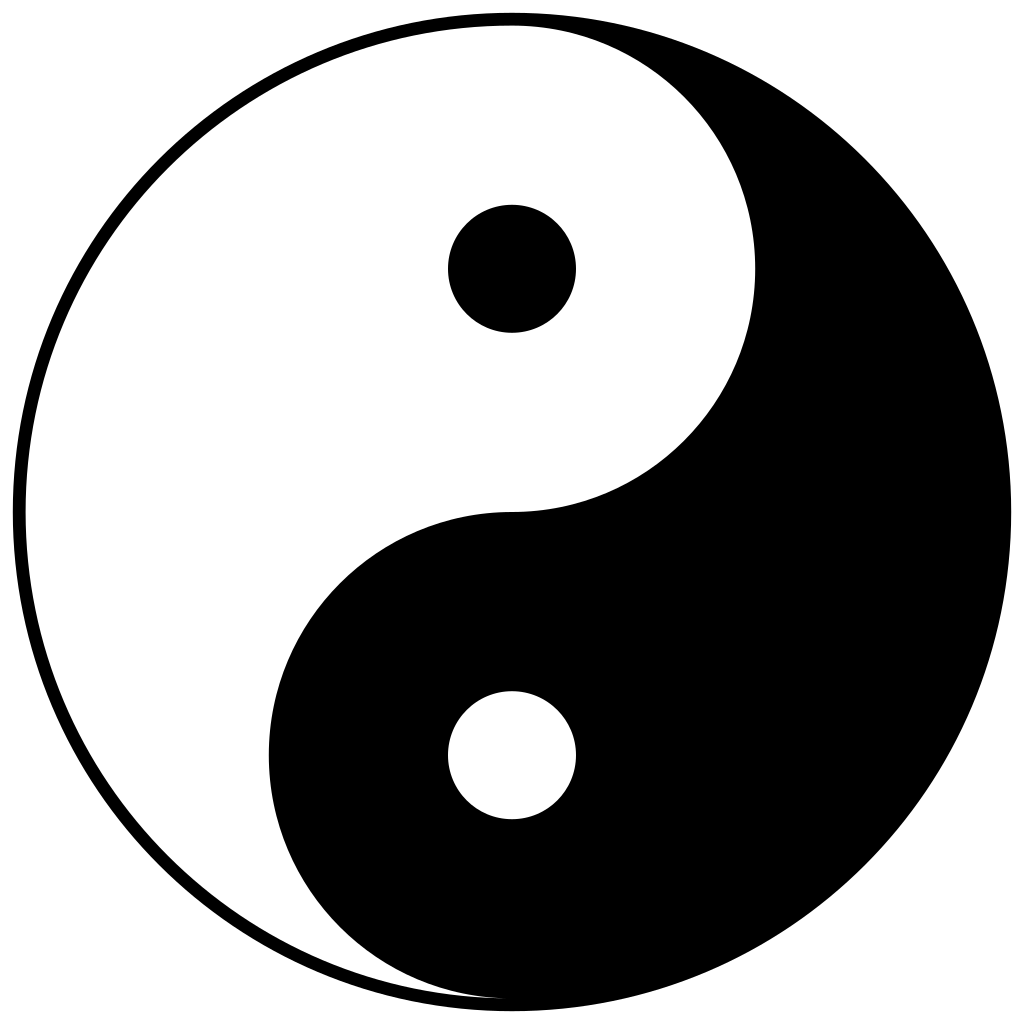
\includegraphics[width=0.95\linewidth]{images/Libro-img058.png}
  \begin{minipage}{\linewidth}
    \caption{Di Gregory Maxwell - From File:Yin yang.png, converted to SVG by Gregory Maxwell., Pubblico dominio, \raggedright\url{https://commons.wikimedia.org/w/index.php?curid=364239}}
  \end{minipage}
\end{wrapfigure}
Secondo il Wu Wei, il non agire, tutto è yin o yang. In questo simbolo, nel punto massimo delle due facce c'è un puntino opposto. Tutto si espande e si contrae, ciclicamente, come un onda. Nelle arti marziali cinesi, non solo si aspetta, ma si da forza al lato sfavorevole per accelerare il cambio di paradigma. Se una persona è molto più forte di noi e ci sta dando un pugno, ci spostiamo e tiriamo il suo pugno nella direzione in cui sta andando in modo che sia ancora più forte e, così da cercare di farlo sbilanciare. Quando si parla di tao, credo si parla di questioni piscologiche ed esistenziali e meno di questioni pratiche. 
Alcuni vivono senza perdersi nei pensieri e nei sentimenti sulla vita, mentre altri vengono travolti dalle circostanze, così tanto da non avere più nulla di autenticamente proprio. Ben presto potresti non riuscire più a distinguere se i vostri pensieri provengono davvero da voi o se è stata la vita a instillarli dentro di voi senza una vostra valutazione consapevole. 
Il tao appartiene ai Principi della non-dualità: non si può né trovare né perdere. Mentre ogni dualismo esclude qualcosa, il tao è un'unica realtà che include tutto. Anche quando pensi al passato o al futuro, lo fai sempre nel presente. Non esiste un modo giusto o sbagliato di vivere in accordo con il tao: siamo sempre parte di esso. La fuga fuori di sé è fuga verso di sé.
È composto da coscienza e mente, desiderio e pace, rabbia e amore, virtù e vizio, sentimenti di gioia e paura, riflessioni profonde e preoccupazioni quotidiane, beatitudine e tormento, compassione e disagio. Vivere è questo, e non c’è un modo corretto o scorretto. Bisogna solo vivere come si è sempre vissuto.
Non va confuso però con la falsa libertà del “fare ciò che si desidera”: la vera libertà include la capacità di fare anche ciò che non si desidera. Essere liberi solo di fare ciò che ci piace significa essere ancora legati al dualismo, prigionieri dei nostri capricci.
Se desideriamo il piacere, una volta raggiunto avremo bisogno di un piacere ancora maggiore per continuare a chiamarlo tale. Nel taoismo, il piacere è legato alla sofferenza e alla miseria. Così si cerca di liberarsi dal desiderio, ma anche questo può diventare un desiderio. Più abbiamo e più cose e pensieri abbiamo da gestire.

Favore e disgrazia non sono da desiderare: la disgrazia per ragioni evidenti, e il favore perché ci potrebbe esporre alla paura di perderlo, che si tratti di reputazione, identità, corpo, sé, denaro o qualsiasi altra cosa.
Dove non c'è attaccamento, non c'è afflizione.
In un saggio, egoismo e altruismo coincidono spontaneamente: l’altruismo nasce senza sforzo, perché privo di ambizione.
Proprio per questo, il saggio è colui a cui si può affidare il mondo, o persino un impero, perché agirà secondo giustizia, non secondo interesse.

Desiderio e non-desiderio non sono opposti: sono la stessa cosa, proprio come l’onda e il mare.
Laozi non invita semplicemente a smettere di identificarsi con l’onda per riconoscersi nel mare, nella propria vera natura. La sua affermazione è più sottile.
Laozi ci dice: vivi pienamente nel mondo della manifestazione, nel regno delle cose e del desiderio, ma con consapevolezza. Vivi nel mistero, nell’indivisibile, in quello stato che è oltre il desiderio e, al tempo stesso, non separato da esso.

Nel momento in cui non credi alle persone, le rendi bugiarde.
Nel momento in cui perdoni le persone, le hai prima rese colpevoli.
Una persona nella pratica può essere davvero colpevole o meno, ma se siamo precipitosi nei giudizi, un ipotesi, nel nostro mondo interiore, la percepiamo come la vera realtà.

Se cerchi di essere umile, rischierai di non esserlo. L’atto stesso di cercare l’umiltà nasce da una forma sottile di orgoglio.
E anche il desiderio di eliminare il desiderio non è esso stesso un desiderio, che può contribuire ad alimentare la sofferenza.

Ogni atto di definizione o valutazione non si limita a descrivere la realtà: la altera, la trasforma, la ricrea a propria immagine nella nostra percezione.

Se cerchi il nirvana come non-desiderio, non lo stai veramente perseguendo, ma lo vedi come una nuova forma di piacere, lontana dalla sua vera natura. Perciò, il taoismo è come un occhio che tenta di guardarsi da sé, o una bocca che prova a mordersi, tentativi impossibili. Il Tao non può essere pienamente compreso con la mente razionale, ma può essere vissuto e percepito intuitivamente.

L’attaccamento alla vita, inteso come brama di possesso e paura della perdita, è il suo peggior nemico.
Vivere con frenesia e bramosia ti fa scivolare via l’esistenza tra le dita, come sabbia. Si rischia così di perdere la pienezza del presente e di giungere alla fine del percorso senza averlo pienamente vissuto con consapevolezza.

\begin{mdframed}[linewidth=1pt]
L’autentico uomo dei tempi antichi non si ribellava contro la povertà, non si inorgogliva dell’abbondanza e non faceva progetti. Un uomo così fatto poteva commettere un errore e non rimpiangerlo, poteva incontrare il successo e non curarsene... L’autentico uomo dei tempi antichi dormiva senza sogni e si svegliava senza preoccupazioni. Mangiando era indifferente ai sapori e il suo respiro veniva dal profondo. Respirava con i calcagni, mentre la massa degli uomini respira solo con la gola... L’autentico uomo dei tempi antichi non amava la vita né odiava la morte. Veniva al mondo senza esultanza, se ne andava senza protestare. Con il cuore leggero arrivava e con il cuore leggero se ne andava, questo era tutto. Non dimenticava donde era venuto, né cercava di sapere quando vi sarebbe ritornato. Allegramente accettava la vita e pazientemente ne aspettava la fine. Questo si chiama non permettere alla mente di deviare dal Dao e non cercare di sostituire l’umano alla natura. Un uomo così fatto si può chiamare un uomo autentico...

Testo tratto da Zhuangzi di Zhuang Zhou 
\end{mdframed}

Il maestro Linji diceva di non sforzarsi ad essere qualcuno, ma di diventare una persona semplice, che non ha impegni, libera da vincoli. Chiunque, anche una persona impegnata, può imparare a notare la bellezza che lo circonda. Tuttavia, la semplicità e il rallentare possono facilitare questa apertura. Questa è una visione forse troppo radicale per noi occidentali, ma più che mai attuale! Se dovessi rileggerla ai tempi nostri, attraverso la lente della non dualità, dove vediamo la persona impegnata come più meritevole di quella non impegnata, possiamo vedere che in realtà sono giuste entrambe le cose e se vogliamo avere solo alcuni impegni e altri no, va bene ancora una volta.
Qualunque cosa allora farai, come tu la vuoi, sarà sempre bene, se non nuoce agli altri o all'ambiente. Più in generale, nel taoismo, l’armonia nasce da azioni spontanee e naturali e, queste si manifestano quando l’individuo è in equilibrio interiore e in connessione con il tutto, non semplicemente quando fa ciò che vuole.
Ma allora quando è giusto fare uno sforzo e quando no? Studiare o allenarsi possono essere attività impegnative, a seconda del piacere che si prova nel farle. Per questo ha senso il consiglio di svolgere le cose senza forzature, includendo anche attività faticose che, nel complesso, si affrontano volentieri. Se qualcuno frequenta l'università, non tutti gli esami saranno piacevoli, ma talvolta abbandonare il percorso di laurea sarebbe uno sforzo ancora maggiore rispetto al superare un esame poco gradito.
Possiamo abbandonare l'idea di mirare a un risultato. Se un taoista prende l'autobus è chiaro che ha una destinazione fisica. Qui si parla di risultati nella sfera morale e spirituale: qualità come bontà, pace, equilibrio mentale, felicità, carattere, coraggio, e così via.
Sull'accettazione dei sentimenti: quando siamo troppo orgogliosi per piangere o troppo spaventati per innamorarci, quale di questi sentimenti dovremmo accogliere? Il dolore o l'orgoglio? La paura o l'amore?
La stessa domanda vale per l'accettazione o il rifiuto del sé: quale parte dovremmo ascoltare? Secondo il taoismo, non dovremmo scegliere, perché è una scelta impossibile. Di fronte a un pericolo, è naturale agire, ma nelle domande esistenziali senza risposta, prendere una decisione non è sempre possibile.
In questo senso, possiamo comprendere la "morte dell'ego" quando riconosciamo che, non ostacolando la saggezza dei sentimenti, possiamo permettere che, come il dolore della nascita apre alla vita, anche la sofferenza porti a nuove scoperte.
Meditazione, psicoanalisi, yoga, buddhismo zen, scienza della mente… tutte queste pratiche ci salveranno dal nostro destino ultimo nel nulla? Secondo la filosofia orientale, comprendere che non possiamo fare nulla, può essere un punto di partenza. E ora, cosa succede? Guarda semplicemente. Non provare a ottenere nulla, non aspettarti nulla, non sperare né cercare. Cerca di rilassarti e osserva senza un obiettivo. L’invito è a non attaccarsi alla speranza come desiderio futuro, ma a vivere pienamente l’esperienza presente, lasciando che la trasformazione emerga spontaneamente.
Anche la meditazione va praticata senza troppa intensità, senza la ricerca di un risultato, va fatto solo nella misura in cui ci dà piacere. Questo dice la versione tradizionale, o ciò che ho compreso. Io aggiungerei anche che dobbiamo guardare ogni cosa nella sua interezza, magari sul momento non ci piace, ma sul lungo periodo invece sì o comunque non farla potrebbe essere peggio. Allo stesso modo, se il distacco dalle cose materiali ci provoca sofferenza, probabilmente non siamo sulla strada giusta, o almeno in quel momento.
Siamo soliti pensare che il saggio sia colui che riconosce il divino in ogni cosa, ma se ogni cosa è divina, allora anche l'uomo comune, vedendole, non fa nulla di diverso dal saggio. Questa affermazione è corretta, ma la differenza tra il saggio e l'uomo comune sta nel fatto che quest'ultimo non ne ha consapevolezza. 

Quando tutto il mondo riconosce la bellezza come tale, nasce la bruttezza.
Quando tutto il mondo riconosce il bene come tale, nasce il male.
Lao Tzu

Per comprendere le cose, tendiamo a separarle: difficilmente comprenderemo il corto senza avere un riferimento del lungo. Con alcune questioni più spirituali, filosofiche ed esistenziali non è sempre possibile. 
Se cerchi di unirti con la realtà, il tuo stesso atto di cercare è già parte della realtà. Quindi, possiamo vivere come desideriamo? Se rispondiamo sì o no, rimaniamo intrappolati nella logica dualistica, quella del "tu" che deve raggiungere l'illuminazione.
perché il tao insiste sulla non dualità? Perché non può esserci una dualità? il Tao come la psicologia e la filosofia hanno la problematica di essere oggetto e soggetto, ovvero la mente studia se stessa. 
Così come una lama non può tagliare se stessa, il pensiero, essendo uno strumento per definire, non può definire se stesso.
Se un'onda cercasse di scoprire la sua vera natura, rimarrebbe sorpresa nel sentirsi dire che è fatta d'acqua. Non saprebbe cosa sia l'acqua, perché questo è il contesto in cui può esplorarsi, ma allo stesso tempo lei stessa è parte di quel contesto.

Del Dao non si può parlare, così come non si può parlare della realtà: ciò di cui parliamo non è la realtà stessa, ma soltanto una sua rappresentazione.
La realtà è solo ciò che è. Tutto ciò che conosciamo, descriviamo o crediamo di sapere è una proiezione, una rappresentazione, una descrizione, una mappa, un'immagine, mai il territorio.
È come nel celebre quadro che raffigura una pipa con la scritta: “Questa non è una pipa”. Perché, appunto, non è una vera pipa, ma solo il disegno di una pipa.
Quando il Dao parla del “non-sapere” e dell’imparare a disimparare, ci invita a riconoscere che ciò che chiamiamo “sapere” non è che un perdersi nel labirinto dei nomi e delle forme. Non coglie la realtà, ma solo la sua ombra.
La vera conoscenza (interiore) non si raggiunge accumulando concetti, ma vivendo pienamente. Eppure, nel momento stesso in cui cerchiamo di afferrarla con il pensiero, essa ci sfugge, trasformandosi ancora una volta in rappresentazione. 

Se qualcuno critica il taoismo, sostenendo che non porta a miglioramenti, ci troviamo ancora di un pensiero dualistico, in cui migliorare è visto come positivo e non migliorare come negativo. Al contrario, nel non dualismo non ci sono queste divisioni: se desideri migliorare, va bene; se non lo desideri, va bene comunque.
Non tutti sono destinati a diventare eroi morali o santi celebrati, né tutti possono vagare senza gli obblighi legati alla famiglia. Allo stesso modo, non è dato a tutti essere una moglie generosa o un marito esemplare. E ancora, non tutti hanno la capacità di accettarsi pienamente come farebbe un fatalista sereno, contento di essere una semplice erbaccia senza ambire a diventare una rosa. Alcuni di noi cercheranno, con risultati limitati e forse frustranti, di migliorarsi in qualche modo, senza mai sentirsi appagati con la semplice auto-accettazione. Accettarsi completamente o cercare di cambiare rinunciando all'io, sono scelte ugualmente sterili, perché non garantiscono che il risultato rappresenti davvero la nostra essenza.
Allo stesso tempo, sia l’auto-accettazione che il desiderio di cambiare possono essere strumenti validi di crescita personale.
Non c'è nulla da cercare, siamo già il Buddha, lo siamo già in questo momento.
Si racconta che il Buddha riuscì a trasformare un assassino in un monaco, e un giorno gli chiese di dire che non aveva mai ucciso nessuno. L'ex assassino replicò che non poteva affermarlo perché non era vero, ma il Buddha gli rispose che poteva farlo: da quando aveva iniziato una nuova vita, infatti, non aveva più ucciso nessuno. Questo per farci comprendere che non dovremmo darci delle etichette fisse, poiché siamo in continuo cambiamento e diversi a ogni istante.
Forse avrete sentito dire: "Se incontri il Buddha per strada, uccidilo!" Il senso di questa frase è che non bisogna venerare il Buddha come un’entità separata da noi. Significa uccidere l'idea fissa che ci siamo fatti del Buddha.
Dopo aver fatto colazione, possiamo dedicare tutta la nostra attenzione al lavare i piatti, anziché perderci in riflessioni su concetti distanti come il vivere bene o il senso della vita. Quanto tempo passiamo concentrati su noi stessi e, quanto invece, sul mondo che ci circonda? Vivere il tao significa vivere in armonia con il mondo circostante.

\begin{mdframed}[linewidth=1pt]
Esiste una legge morale dentro di noi?

Immanuel Kant sosteneva l’esistenza di un senso morale innato nell’essere umano. Ma si tratta davvero di una predisposizione naturale, o è la cultura a modellare il nostro giudizio morale?

Uno studio pubblicato su Nature Human Behaviour da Yasuhiro Kanakogi e colleghi dell'Università di Otsuma (Giappone)\endnote{Third-party punishment by preverbal infants. Yasuhiro Kanakogi, Michiko Miyazaki, Hideyuki
Takahashi, Hiroki Yamamoto, Tessei Kobayashi \& Kazuo Hiraki. Nature Human Behaviour volume 6, pages 1234–1242 (2022)
\raggedright\url{https://www.nature.com/articles/s41562-022-01354-2}} ha cercato di esplorare questa domanda coinvolgendo bambini di appena otto mesi, troppo piccoli per aver appreso norme sociali in modo consapevole.
Nel loro esperimento, i bambini osservavano una scena su schermo in cui alcune forme geometriche interagivano: in certi casi una forma “aggrediva” un’altra, facendola fuggire. I ricercatori hanno osservato che i bambini tendevano a focalizzare l’attenzione sulla figura aggressiva e a selezionare (ad esempio tramite tocco o sguardo) la sua rimozione dallo schermo, comportamento interpretato come possibile preferenza per l’eliminazione dell’agente antisociale.

Secondo gli autori, questo comportamento potrebbe riflettere una sensibilità precoce verso atti percepiti come antisociali o ingiusti. Tuttavia, l’interpretazione richiede cautela. È possibile che tali reazioni siano guidate da meccanismi cognitivi generali, cioè processi mentali di base che non implicano necessariamente un giudizio morale. Ad esempio, già nei primi mesi di vita, i neonati tendono a mostrare preferenza per il volto della madre o per suoni familiari: si tratta di reazioni apprese o innate, ma non necessariamente legate a un giudizio di tipo morale.
\end{mdframed}

\subsection{Altri esempi}
Il capitolo potrebbe concludersi qui, ma ho notato ch, anche quando comprendiamo concetti a livello razionale, può essere difficile integrarli nella nostra esperienza quotidiana e nei comportamenti. La ripetizione e l'esposizione prolungata possono facilitare questo processo.
Di seguito vorrei rivedere questi concetti sotto forme diverse. Una cosa che a me ha aiutato oltre a leggere libri sull'argomento è stato iscrivermi a
canali di Youtube, ascoltare podcast di crescita personale. Riascoltare contenuti può favorire l’apprendimento, soprattutto se associato a riflessione attiva e applicazione concreta dei concetti. I libri li trovate sparsi nel libro, tra le note, mentre di seguito le fonti
audio e video che più apprezzo in ordine alfabetico.

\begin{itemize}
\item Daily Cogito con Rick Du Fer: \raggedright\url{https://www.spreaker.com/show/daily-cogito} 
\item Edizioni Riza con Raffaele Morelli: \raggedright\url{https://www.youtube.com/user/EdizioniRiza}
\item PSINEL con Gennaro Romagnoli: \raggedright\url{https://www.spreaker.com/show/audio-newsletter-anl} 
\item Sadhguru: \raggedright\url{https://www.youtube.com/channel/UCVoo2xW\_PFFpdkh9vjexLTg} 
\item Wesa Channel: \raggedright\url{https://anchor.fm/wesapodcast} 
\end{itemize}
E poi sicuramente una menzione speciale per Massimo Recalcati, Tiziano Terzani, Umberto Galimberti e tanti altri che mi
hanno influenzato molto ma non hanno un canale (credo) dove periodicamente pubblicano contenuti. Quindi, vediamo altri
punti di vista su quello che abbiamo detto.

\subsubsection{Consapevolezza}
Quando si parla di consapevolezza credo si parli principalmente di quella che abbiamo verso noi stessi, verso le nostre azioni e
verso i nostri pensieri. Siamo sempre sicuri che i nostri pensieri e le nostre azioni siamo davvero noi stessi? O sono
solo il prodotto di come crediamo che dovremmo comportarci, secondo noi, in una certa situazione o in un certo ambiente? 

Iniziamo a notare: come ci mostriamo agli altri? Come vorremmo che gli altri ci percepissero? Cerchiamo di fare
interventi per sembrare intelligenti, colti? O che vogliono sembrare sprezzanti e spietati sui vari argomenti? Marco
Aurelio ogni sera si prendeva del tempo per rivedere i modi in cui ha agito, per chiedersi, perché ho fatto ciò che ho
fatto? Qual è il bisogno che sta dietro alle mie azioni? 

Spesso sono i gruppi di appartenenza a richiederci certi comportamenti e pensieri,
dall'appartenenza sportiva, musicala, politica, religiosa ecc…

Io per esempio fin dalle scuole superiori ho fatto parte di tanti gruppi, ma in modo marginale, per esempio,
ascolto musica rap ma ero l'unico a non bere alcol e fumare, anzi, sono un salutista,
questo perché sono anche un appassionato di sport, mi piacciono tutti, ma allo stesso tempo faccio un lavoro sedentaio, dove ci sono alcuni classici “nerd” che nell'immaginario collettivo non fanno attività fisica, giocano alla play station, a Dungeons \& Dragons e giochi di ruolo, attività che non pratico. Così in maniera contraddittoria passo dal ragazzino tossico disadattato quando
vado in skate, a pedante moralista quando scoprono che sono vegetariano, a fanatico esaltato quando esco dalla palestra
e, nerd solitario quando è il lato informatico a venire fuori.
Anche quando le nostre azioni, come delle scelte alimentari, non creano problemi agli altri, spesso ho sentito pressioni perché le cambiassi.
Le scelte non convenzionali possono destabilizzare gli altri poichè tendono a mettere discussione le loro scelte.

Il fenomeno della conformità sociale è stato osservato da alcuni esperimenti, uno dei primi esempi è stato realizzato nel 1962 da Candid Camera, un programma televisivo americano che faceva scherzi nascosti ai malcapitati. In una sala d'attesa, tutti gli attori si alzavano al suono di un campanello, tranne una persona ignara. Dopo qualche minuto, anche la vittima si alzava, seguendo il gruppo. Poi, gli attori uscivano uno per uno, lasciando la vittima da sola. Alla fine, anche quando non c'era più nessuno nella stanza, la vittima continuava ad alzarsi al suono del campanello.

Ad esempio nella politica, è improbabile trovare un partito che in tutte le sue proposte rispecchino, nella loro totalità,
 tutti i nostri pensieri e le nostre idee. I veri seguaci di un partito però difenderanno spesso quei pensieri, come se
fossero i loro, è quello in cui credono, talvolta nascondendo così tanto a loro stessi la vera idea che hanno a riguardo. Se si
dovesse fare loro un discorso simile, ponendo l'ipotesi che potrebbero non essere
d'accordo con tutte le idee promosse dal partito, potrebbero rispondere che loro sono davvero così, che
credono davvero a tutti i punti proposti. Questa risposta sarebbe anche realmente genuina, perché nella loro parte
conscia è davvero così. Anche per questo sarebbe meglio non darsi etichetta, sono di destra, sono di sinistra o
qualsiasi altra. La mancanza di consapevolezza ci porta a pensare e comportarci nel modo appreso
dall'esterno, dalla società, senza esserci interrogati se andasse bene anche a noi o se lo ritenessimo giusto.
Se qualcuno dovesse mangiarsi una pizza all'ananas, non sarebbe infrequente assistere ad un scena di sfottò generale verso quella persona. Anche persone della tavolata che hanno appena conosciuto, potrebbero partecipare alla presa in giro, perché si può fare, perché su questo siamo tutti d'accordo che è legittimo canzonare. Ma perché? che problema ti da? di esempi se ne potrebbero fare tanti, ma la domanda è: quante sono le cose che ci agiscono? Se non si fa un ragionamento semplice come: perché è un problema? di quante altre cose re-agiamo senza che ci sia a separare stimolo e azione un nostro filtro, un nostro ragionamento, la nostra persona o quella che vorremmo diventare?

Sul web si nota un'esplosione di etichette di appartenenza che da una parte sono positive, per chi le sa dare, come ad esempio i medici, ma dall'altra parte possono essere negative perché ci deresponsabilizzano dalla ricerca, potremmo dire: mi hanno trovato, io appartengo a questo!
A volte non vogliamo trovare la nostra identità, ma appartenere. 

A volte succedono cose più sottili, come la frase che spesso si sente dire: “io dico quello che penso!” Frase che porta
con se un immaginario collettivo positivo fatto di onestà, verità, coraggio, integrità e non aver paura di fare la cosa
giusta. Siamo tutti d'accordo su questo no? L'ideale è mettere in discussione
anche una verità così assodata e infatti, come spesso accade, la risposta è: dipende. Poche cose sono assolute, sempre
vere o false. Per esempio potremmo avere a che fare con una persona, prendiamo il caso di un collega o di un assessore
comunale da cui attendiamo certi documenti, o una firma. Questa persona potrebbe essere supponente, arrogante,
maleducata e irritante. La relazione che abbiamo con questa persona è solo di natura professionale, una volta che ci
avrà fornito quello di cui abbiamo bisogno, magari non la sentiremo mai più nella vita, quindi ha senso dire quello che
pensiamo? Qual è il fine? Riuscire a sistemare un rapporto che tanto non ci interessa avere? O forse serve solo a
sfogarci? O per poter dire a noi stessi che non abbiamo paura di dire le cose in faccia alla gente? Ma
l'obiettivo non era ricevere una documentazione firmata? In quale modo dire che lui non è una
persona che ci va a genio può velocizzare la produzione e la firma di questi documenti? Questi sono i casi in cui entra
il pilota automatico dell'inconsapevolezza, rischiando di non essere più noi al comando.

Quindi anche una verità che diamo per assodata come questa, ovvero il dire sempre e comunque quello che pensiamo, può
essere controproducente al nostro obiettivo finale. Questa persona potrebbe offendersi, arrabbiarsi, anche se
oggettivamente abbiamo ragione e, per rappresaglia dichiararci guerra e metterci i bastoni fra le ruote. In questo caso
forse sarebbe meglio fare buon viso a cattivo gioco, ottenere i documenti e, poi comunque, tenerci le nostre opinioni
personali per noi, perché in un futuro potremmo ancora avere bisogno di quella persona.

l'Io non è padrone in casa propria. - Sigmund Freud

Ma perché c'è questa discrepanza tra il mondo reale, interiore e esteriore, e quello che crediamo
essere il mondo? Perché il nostro cervello non ha un accesso diretto a questi mondi, trovandosi intrappolato nella
scatola cranica può fare ipotesi interpretando le informazioni che gli arrivano attraverso i cinque sensi. 
Se sentiamo una sensazione allo stomaco,
potrebbe essere fame, ulcera, ansia, un trauma, nostalgia, amore o mille altre cose. Ad esempio eccitazione e ansia
provocano sensazioni corporee molto simili. Per cui quando sentiamo l'ansia potrebbe trattarsi di eccitazione. Quindi il nostro cervello potrebbe dare un'interpretazione errata magari perché va in contrapposizione con
dei valori sociali e di conseguenza potrebbe influenzare un malessere come l'ansia. Questo può contribuire, ma non è l’unica causa, alla comparsa dell’ansia. Allo stesso modo quando ci innamoriamo
potremmo provare angoscia e il malessere nel non conoscere i desideri dell'altra persona nei nostri confronti. 
Così, in quel momento noi potremmo scambiare queste sensazioni e credere che se proviamo angoscia e, non amore e, che quindi non sia la persona giusta per noi. Viene chiamata granularità emotiva quando il cervello cerca di dare un senso alle sensazioni 
fisiche\endnote{\raggedright\url{https://youtu.be/v5hWwUBrv0o}}. 

\begin{mdframed}[linewidth=1pt]
Consigli per dormire

Il dormire bene è diventato un argomento molto attuale date le screscenti difficoltà legate al
sonno. Solitamente la grossa difficoltà nel prendere sonno è legata ai pensieri, dove si
organizza la giornata successiva, si pianifica e ripensa alle cose successe. Questo ci attiva mentalmente e,
quando ci accorgiamo, iniziamo a pensare che se non riusciremo a prendere sonno velocemente, non riusciremo a riposare
a sufficienza e l'indomani saremo stanchi. Questo però ci attiverà ancora di più, entrando così in
un loop dove più ci sforzeremo di dormire e più difficilmente ci riusciremo. Come sappiamo non possiamo pensare di smettere di
pensare, ma possiamo pensare ad altro, come ad esempio portare l'attenzione sul nostro corpo o sul
nostro respiro. 

Quello che funziona per me, è portare l'attenzione sulle immagini. Quando chiudiamo gli occhi vediamo nero, ma se
facciamo un po' di attenzione, almeno nel mio caso, vedremo delle macchie, delle forme irregolari, bianche o
leggermente colorate. Osservando queste forme, come si muovono e come mutano, con un po' di tempo
e pazienza diventeranno sempre più complesse, assumendo forme razionali di persone e paesaggi. Si potrebbero sentire anche
dei dialoghi senza molto senso ad un certo punto. Se riusciamo ad osservare queste immagini e suoni senza cercare di
controllarli per dargli una forma prima del tempo, ma osservandoli semplicemente come un film, non so il perché, ma
questo mi aiuta a prendere sonno in poco tempo.

L'esercito americano utilizza una tecnica che li aiuta ad
addormentarsi rapidamente anche in luoghi e situazioni difficili. Può richiedere un paio di settimane di pratica ed è stato
sviluppato da Lloyd Winter. Fase 1: rilassare ogni parte del proprio corpo, partendo
dal viso (lingua compresa) fino alle gambe, respirando lentamente. Fase 2: ripulire la mente immaginandosi sdraiati in
una canoa su un lago calmissimo, sotto il cielo blu e senza nulla intorno, oppure avvolti da un'amaca di velluto nero
in una stanza completamente buia\endnote{\raggedright\url{https://www.focus.it/scienza/salute/meglio-dormire-insieme-o-da-soli}}.

Un consiglio che ritrovo spesso è quello di
fare attività rilassanti una o due ore prima di andare a letto. Si consiglia anche di non utilizzare schermi prima
di andare a letto e preferire attività come la lettura. Se l'addormentamento non avviene entro circa 20 minuti, può essere utile alzarsi e dedicarsi a un'attività rilassante fuori dal letto. L'obiettivo è evitare che il letto venga associato alla veglia o ad attività diverse dal sonno.

Meglio dormire con qualcuno o da soli? Sembra che chi dormi con
il partner riesce a farlo più velocemente, non ha risvegli frequenti durante la notte, né si sveglia troppo presto al
mattino, dorme di più e ha un minor rischio di insonnia. Queste sono le conclusioni a cui è giunto Brandon Fuentes
dell'Università dell'Arizona, inoltre sono stati registrati un minor grado di depressione, ansia e stress e una
maggiore soddisfazione della vita in generale. 

Quello che poi rende difficile addormentarsi è lo sforzarsi di dormire, il pensare a come riuscirci, preoccuparsi che il giorno dopo saremo stanchi. Sembra che il rimanere sdraiati con gli occhi chiusi, comunque riposi il nostro corpo, il sonno serve fondamentalmente per permettere al cervello di rielaborare e fissare ciò che è successo nella giornata. Il sonno è comunque una fase di importanza primaria, ma magari sapere questa informazione ci può consentire di stare più sereni e pensare meno al sonno in modo che arrivi più facilmente. 
Infine se si ha dormito male, secondo uno studio pubblicato sulla rivista Physiology \& Behavior\endnote{\raggedright\url{https://www.sciencedirect.com/science/article/pii/S0031938423003347}}, possono aiutare 20 minuti di movimento per recuperarsi.

Cose da NON fare prima e durante la messa a letto:

\begin{itemize}
\item Pianificare la giornata di domani e avere pensieri attivanti
\item Guardare uno schermo (Tv, smartphone, tablet ecc… nei 30 minuti prima di dormire)
\item Riposini pomeridiani
\item Attività stimolanti
\item Bevande alcoliche, caffeina, thé, energizzanti o alimenti ricchi di zuccheri
\item Valeriana e camomilla non hanno forti evidenze sulla loro efficacia
\item Fumo
\item Sport
\end{itemize}

Cose da fare prima e durante la messa a letto:

\begin{itemize}
\item Rimuovere luci dalla stanza, anche con una mascherina
\item Rimuovere i rumori dalla stanza, anche con dei tappi o del rumore bianco
\item Andare a letto e svegliarsi più o meno alla stessa ora, dormendo circa 7/8 ore
\item Bere del latte caldo o fare un bagno caldo può favorire il sonno
\item La temperatura della stanza dovrebbe stare tra i 18 e i 21°
\item Mangiare leggero e due ore prima di andare a letto
\item L'attività fisica regolare favorisce il sonno, ma evitandola di sera
\item Avere un letto comodo 
\item Nascondere orologi e sveglie, che mettono pressione sul dormire in fretta
\end{itemize}
\end{mdframed}

\subsubsection{Desideri}
In un intervista di Carl Gustav Jung a un capo indiano, emerse da quest'ultimo che guardando i
bianchi, notava spesso sui loro volti un espressione di tensione e ansia, come se fossero sempre alla ricerca di
qualcosa, senza però sapere di cosa sono in cerca. Secondo il Buddha, la radice della sofferenza si trova nell’attaccamento e nella bramosia (tanhā), ovvero nel desiderio compulsivo e nel volere che le cose siano diverse da come sono.

Il problema è che senza desiderio, senza quella scintilla, quella voglia di fare, forse non ci sarebbe vita ma solo
sopravvivenza. Il paradosso è che il desiderio sorge spontaneo, non decidiamo di avere
un desiderio. L'altra contraddizione è che il desiderio porta angoscia ma senza desiderio non c'è vita perché è uno dei motori che ci muove e ci fa agire. 

Il desiderio, una volta appagato, spesso lascia spazio al bisogno di un nuovo oggetto da desiderare. Secondo alcune prospettive filosofiche, il desiderio è fine a se stesso.
L'oggetto del desiderio è il desiderio stesso. Quando ti innamori desideri che anche
l'altra persona ti desideri. Non bisogna quindi sentirsi inadeguati né quando non desideriamo più
un oggetto né quando ci sentiamo inquieti\endnote{\raggedright\url{https://www.youtube.com/watch?v=sMReYx6qrfo}}.

Sembra che siamo quindi in trappola, senza possibilità di scappare, ma forse una via di fuga c'è.
Spesso trattiamo il desiderio come un bisogno. Con questo non voglio dire che il desiderio sia meno importante del
bisogno, anzi, è una spinta vitale importante.

Tutto quello che facciamo nella vita non è un modo per essere amati un po' di più? - Dal film “Prima dell'alba”

\begin{mdframed}[linewidth=1pt]
Gli scimpanzé risentono dell’“effetto pubblico”?

Negli esseri umani, la presenza di spettatori può influenzare le prestazioni, migliorandole o peggiorandole. Un gruppo di ricercatori dell’Università di Kyoto ha indagato se anche i primati non umani fossero soggetti a questo fenomeno, spesso legato al desiderio di mantenere una buona reputazione.

Per scoprirlo, hanno analizzato migliaia di sessioni in cui, nell’arco di sei anni, degli scimpanzé hanno svolto compiti al computer tramite touch screen. I risultati hanno osservato che la loro performance variava in base al numero di persone presenti ad osservarli.

In particolare, quando il compito era semplice, gli scimpanzé ottenevano risultati peggiori se osservati da più sperimentatori o da individui a loro familiari. Al contrario, se il compito era più complesso e richiedeva maggiore concentrazione, le loro prestazioni miglioravano progressivamente con l’aumento del numero di spettatori, portando anche a una maggiore gratificazione.

Gli studiosi hanno osservato che l'influenza della presenza di un pubblico potrebbe essersi evoluta prima della comparsa delle società umane.
\end{mdframed}

Possiamo vedere il desiderio come un viaggio piacevole, ad esempio potremmo affezionarci
 all'andare in palestra e non all'avere i muscoli o al piacere della scoperta più che al mostrare di
 sapere tante cose. Anche se il nostro desiderio non è soddisfatto in quel momento, va bene lo stesso, anche perché, una volta soddisfatto un desiderio, potrebbe sorgerne uno nuovo. Siamo noi, come ci suggerisce Epitteto
che diamo un certo significato alle cose: sarò felice solo quando avrò soddisfatto quel desiderio. Mentre in realtà
quando raggiungiamo un obiettivo siamo soddisfatti e non va quindi necessariamente confusa con la felicità. Anche
l'ammirazione degli altri, che è qualcosa di esterno a noi, è un miraggio, ci appaga ed è
importante sentirsi apprezzati, difficilmente ci dona la felicità. I sogni sono dei motori per la nostra vita ma non vanno
trasformati in aspettative, pretese e condizioni necessarie alla felicità.

“La mancanza di qualcosa che si desidera è una parte indispensabile della felicità” - Bertrand Russell

Spesso il desiderio nasce dalla tendenza della mente a cercare appagamento nel futuro o in qualcosa di esterno a sé. Tuttavia, alcuni desideri possono anche essere espressione consapevole e presente dei propri bisogni autentici. Se
credo di essere i miei pensieri, rischio di diventare questi desideri, questi bisogni, mancanze, attaccamenti e avversioni. Anche il
desiderio di trovare l'illuminazione rischia di diventare un ulteriore brama di appagamento o completamento nel
futuro. A volte è bello sognare ad occhi aperti su come vorremmo la nostra vita e, ricordare i bei momenti passati, ma può essere
pericoloso se fatto inconsapevolmente, questo perché potremmo cadere nella nostalgia, o in aspettative e desideri che potrebbero non realizzarsi, attaccamento su qualcosa che non ritornerà, idealizzazioni di qualcosa che ormai esiste solo nella nostra mente e forse non è mai esistito. Magari abbiamo creato un immagine attorno a una certa cosa, una certa persona, un certo momento della nostra
vita che abbiamo idolatrato e, mitizzato, a tal punto da creare una distorsione che nella realtà non era così perfetta.
Altre volte invece ottieni quello che volevi, ma non era come te lo immaginavi, nel tuo sogno era più bello e questo
porta a un forte sconforto. Porta l'idea erronea che quindi non riusciremo ad essere felici e, invece, possiamo esserlo già ora, anche se le condizioni non sono perfette. Ridefiniamo il modo in cui chiamiamo le emozioni:
quello che provo adesso magari è felicità, quando sono agitato magari è eccitazione e così via…

Il passato e il futuro
esistono solo nella nostra mente, se noi prestiamo attenzione al passato o al futuro, difficilmente riusciremo a prestarla al presente. Con questo non voglio dire che non si debba pensare più al futuro. Portare la propria attenzione al futuro serve a pianificare. Nel futuro, le nostre proiezioni possono suscitare cose che possono andare bene o male, quindi speranza o ansia. Spesso i sentimenti negativi non sono legati a una minaccia immediata nel presente, ma piuttosto a pensieri sul passato o sul futuro. È giusto ripensare a quello che è successo per evitare che in futuro si ripeta. Ma ho scelto di pensarci o la mia compulsione mi sta facendo pensare?
Poche cosa sono definitive, irrisolvibili, se sentite che al lavoro o la società
vi sta chiedendo troppo e, avete paura di non riuscire a tenere il passo, chiedetevi, cosa succederebbe se mollaste?
Tante volte le risposte che ci diamo, non sono sicuramente piacevoli, ma nemmeno così terribili o irrisolvibili. Se si riesce a ottenere un minimo di sollievo da questa concezione si
riuscirà ad affrontare le varie sfide che la vita ci pone davanti con più serenità a probabilmente senza arrivare
nemmeno a mollare. Alcune volte abbiamo paura di avere paura, dell'ansia, dello stress, di non
essere felici in quel particolare momento, credendo che sarà per sempre, più che del motivo vero che ci sta dando
preoccupazioni.

Uno studio condotto su persone con ansia generalizzata ha osservato che circa il 91\% delle loro preoccupazioni non si è mai realizzato. Questo suggerisce che gran parte delle paure mentali possono essere sproporzionate rispetto alla realtà, anche se il dato non si applica automaticamente a tutti.\endnote{\raggedright\url{https://www.sciencedirect.com/science/article/abs/pii/S0005789419300826}}

“Se c'è soluzione, perché ti preoccupi? Se non c'è soluzione, perché ti preoccupi?” - Aristotele.

Immagina di continuare a vivere la vita nel modo in cui hai sempre vissuto, ma senza tutta l'eccessiva importanza e tutta l'ansia, lo stress, la preoccupazione, ecc… La cose alla peggio andrebbero come sono sempre andate e, hai dimostrato di saperle gestire. Forse accettando questo, prendendoci meno sul serio, senza tutta questa premura, dovere e obbligo di trovare la serenità potremmo davvero riuscire a vivere sereni.

Dovremmo cercare di rimuovere quell'obbligo di uno scopo. Quando camminiamo, ad esempio, potremmo sentirci parte del panorama che ci circonda e dell'azione che stiamo compiendo.
Non siamo qualcuno che va da qualche parte: siamo noi stessi immersi nel l'atto del camminare. 
Cerchiamo di fare le cose più lentamente del normale.

\begin{mdframed}[linewidth=1pt]
La distrazione sul posto di lavoro può avere effetti benefici. Alcuni studi suggeriscono che brevi pause con contenuti piacevoli, come video divertenti, possono migliorare l’umore e facilitare il ritorno al lavoro dopo situazioni stressanti, con possibili benefici indiretti sulla produttività. Questa è la conclusione di un team internazionale di ricercatori provenienti dal Trinity College di Dublino, dall'Università della Florida e da diverse istituzioni accademiche tedesche e austriache\endnote{Why silly distractions at work can actually be good for you \raggedright\url{https://www.tcd.ie/news_events/articles/why-silly-distractions-at-work-can-actually-be-good-for-you-/}} \endnote{Workplace distractions are good for you. - Trinity College Dublin \raggedright\url{https://www.tcd.ie/business/news--events/2022/workplace-distractions-are-good-for-you-/}}.

Secondo lo studio, l'indulgere in attività divertenti durante la giornata lavorativa può fungere da antistress. L'analisi ha osservato che quando l'attività di distrazione è piacevole, come guardare un video divertente su YouTube, il carico cognitivo derivante da compiti stressanti viene alleviato. Durante uno studio condotto su un campione di 85 dipendenti per 12 giorni consecutivi, i partecipanti hanno ricevuto occasionalmente video o testi dal contenuto allegro. È emerso che questi "distrattori", quando visionati subito dopo eventi stressanti come email fastidiose o conflitti con superiori o colleghi, contribuivano a migliorare l'umore e a riprendere il lavoro con rinnovato slancio.

Lo studio suggerisce che brevi pause con stimoli positivi possono aiutare a gestire momenti stressanti. Questo potrebbe, in teoria, favorire anche un maggiore coinvolgimento e relazioni più armoniose.

Numerosi studi scientifici internazionali hanno osservato che l’aumento del rumore nei luoghi di lavoro è correlato a un incremento dei livelli di stress tra i lavoratori e a un peggioramento delle loro performance. La letteratura sottolinea come il rumore ambientale, soprattutto quando supera certi livelli, possa provocare una risposta fisiologica di stress, con effetti negativi sia sulla salute mentale che fisica. Allo stesso tempo, il rumore influisce negativamente sulle capacità cognitive, riducendo in molti casi, la concentrazione, aumentando gli errori e abbassando la produttività. Questi effetti sono stati osservati sia in ambienti industriali che in uffici, e risultano particolarmente marcati nei compiti che richiedono attenzione sostenuta e precisione. In sintesi, la ricerca scientifica suggerisce che ambienti di lavoro più rumorosi sono associati a maggiori livelli di stress e a una diminuzione delle prestazioni lavorative \raggedright\url{https://www.ncbi.nlm.nih.gov/pmc/articles/PMC8511314/} \raggedright\url{https://www.sciencedirect.com/science/article/pii/S0160412021002268} \raggedright\url{https://www.frontiersin.org/articles/10.3389/fpsyg.2018.01354/full} \raggedright\url{https://www.ncbi.nlm.nih.gov/pmc/articles/PMC6503768/}.
\end{mdframed}

Per essere felici bisogna credere anzitutto nella possibilità di esserlo: Io adesso ci credo - Lev Tolstoj 

Anche qua, credo che la verità stia nel mezzo. Entrambe le teorie sono vere, credo che la vera discriminante sia la
consapevolezza. L'essere umano tende ad avere desideri infiniti per sua stessa natura e, agevolata
dall'ambiente. Tante volte ci diciamo che per essere felici dobbiamo trovare un partner, poi
quando lo troviamo diciamo, no, per essere felici, non serve solo un partner, serve anche un bello stipendio, poi
ottieni anche quello e dici, per essere proprio davvero felici, serve anche una nuova casa e poi
qualcos'altro ancora potenzialmente all'infinito. Nonostante abbiamo sperimentato più
volte tutti noi non essere cosi. Molte esperienze ci mostrano come la felicità non possa derivare solo da fattori esterni. I desideri non sono il problema, secondo Sadhguru la differenza sta nella consapevolezza, quando i tuoi
desideri sono inconsapevoli potremmo chiamarli avidità o compulsione. 

Arthur Schopenhauer diceva che la vita è come un pendolo che oscilla tra dolore e noia.
Quando desideriamo qualcosa, viviamo il dolore e la frustrazione di non avere questo oggetto del nostro desiderio. Così
ci adoperiamo per ottenerlo e quando ci riusciamo, la sensazione di benessere dura solo per poco fino a che non sarà la noia a soppiantarla. La noia può emergere quando si è privi di obiettivi o stimoli, ma anche questa condizione dipende da come si struttura il proprio rapporto con il desiderio e la motivazione.
Secondo questa visione possiamo solo vivere il dolore della noia o quello di un desiderio inappagato o, invece
possiamo, diventando consapevoli di questo aspetto intrinsecamente legato all'essere umano, 
comprendere che non c'è soluzione e, accettarlo… come sappiamo però
l'accettazione non è un processo passivo e, infatti, anche in questo caso, utilizziamo
l'accettazione come processo trasformativo di noi stessi. Ora che sappiamo quanto sia difficile
liberarci da questo meccanismo e, che non siamo sbagliati noi, siamo liberi dall'etichettarlo in
maniera negativa e possiamo ridefinirlo e, sapendo che è normale, possiamo “smascherarlo” e vedere che può essere necessario e
positivo per noi, in quanto il desiderio può utilizzare la frustrazione per portarci all'azione, a
raggiungere i nostri obiettivi e a diventare noi stessi, quando i nostri desideri sono allineati coi nostri valori. Possiamo ridefinire la nostra idea iniziale del tipo: soffro a fare questa cosa
nell'attesa di raggiungere questo obiettivo ed essere felice; in: viaggiare pieni di speranze sia
meglio dell'arrivare. Oscar Wilde dice che "Non c'è nulla di più terribile di
una serie prolungata di giorni felici" proprio perché ci sarebbe la noia, che è di gran lunga
peggiore della frustrazione di un desiderio inappagato. Per questo anche dare troppo ai bambini potrebbe non essere
positivo.

Numerosi studi hanno evidenziato come i musicisti professionisti e V.I.P., le quali vite vengono viste come perfette, soffrano di depressione in percentuali significativamente maggiori rispetto alla media della popolazione, con valori che possono variare da circa il 36\% fino al 69\%. Questi dati osservano una prevalenza di depressione nei musicisti che può essere fino a tre volte superiore rispetto a quella riscontrata nel pubblico generale. Per la popolazione non V.I.P. risulta la prevalenza di depressione si aggira tra il 13\% e il 20\% \endnote{\raggedright\url{https://www.ncbi.nlm.nih.gov/pmc/articles/PMC6472461/}} \endnote{\raggedright\url{https://www.ncbi.nlm.nih.gov/pmc/articles/PMC6361838/}} \endnote{\raggedright\url{https://www.who.int/news-room/fact-sheets/detail/depression}}.

Possiamo trovare questi concetti, trattati da un punto di vista irriverente nel libro: La sottile arte di fare quello
che c***o ti pare\endnote{\raggedright\url{https://www.amazon.it/dp/8822707451}}. Mark Manson spiega che internet e la cultura popolare
tende alla felicità cercando di colmare e portando l'attenzione su ciò che ci manca e non sulla gratitudine di ciò che abbiamo.

Desiderare un'esperienza più positiva è spesso un'esperienza negativa. 
E, paradossalmente, accettare la propria esperienza negativa è spesso un'esperienza positiva.

Il filosofo Alan Watts ha coniato la “Legge d'inversione” che dice proprio questo: 
più ti sforzi di stare continuamente bene, più difficilmente sarai soddisfatto, perché inseguire qualcosa ne rinforza la sua mancanza. Più cerchi di mostrarti forte più rischi di sembrare e sentirti debole, più cerchi sembrare intelligente più rischi di sembrare e sentirti stupido. Se cerchiamo di evitare il dolore, gli stiamo dando troppa importanza. Se diamo importanza a tutto e a tutti, crederemo di
meritare sempre la felicità e che tutto vada come vorremmo, così potremmo vedere ogni avversità come un ingiustizia o
un'offesa personale. Così il ricco può soffrire a causa delle sue ricchezze e il povero per la sua
povertà. Chi insegue i piaceri mondani rischia di soffrire a causa di tali piaceri e, chi si astiene da essi può soffrire per la loro
mancanza. Non tutte le sofferenze sono uguali ma provare un po' di sofferenza è frequente e normale.
Questo non ci deve far cadere nel nichilismo, perché se mi abituo a vedere tutto come senza importanza, anche le cose belle, le potrei vedere in questo modo, rischiando di renderci meno sensibili.

Il segreto sta nella risoluzione dei problemi, non nella loro assenza. Per essere felici, spesso, abbiamo bisogno di qualcosa da
risolvere. La felicità è una forma di azione, non qualcosa che ci viene donata passivamente, o che scopriamo come per
incanto. Per vedere se le nostre azioni sono ben indirizzate, possiamo saper valutare correttamente i feedback. Se
ricevo pochi messaggi dal mio partner e ne deduco che questo sia sintomo di una brutta relazione, dovrei, prima di
trarre questa conclusione affrettata, domandarmi se questo metro di giudizio e significativo. Il piacere può essere un
indicatore pericoloso. L'esperienza di chi sviluppa dipendenze, ad esempio, dimostra come la ricerca ossessiva del piacere possa portare a esiti distruttivi anziché al benessere. Chi concentra la propria energia sui piaceri superficiali può rischiare di diventare più ansioso, più emotivamente instabile e più depresso. Delegare il nostro benessere a elementi esterni a noi può essere disfunzionale, in quanto fuori dal nostro controllo, come il piacere sempre e a tutti. Se invece tendo a migliorare la mia vita sociale, posso continuare a fare buone azioni,
indipendentemente da cosa gli altri avrebbero preferito e dalla loro interpretazione o reazione. In generale, gli
obiettivi esterni o al di fuori della nostra influenza, possono essere più pericolosi. Alcuni dei valori più stabili e salutari sono quelli che consentono gratificazione già nel percorso, non solo nel traguardo.

Per Karl Popper: "La vita è una serie di problemi da risolvere". Questa
caratteristica umana da cui è difficile prendere le distanze, non va vista quindi come qualcosa da accettare con rassegnazione,
come abbiamo visto, è grazie a questa qualità che rende viva l'esistenza, ci da infinite
possibilità di agire, conoscerci, sviluppare nuove abilità, fiducia in sé, va quindi visto con entusiasmo e non come
una condanna.

Agostino d'Ippona diceva di imparare ad amare quello che si ha già, in modo da svuotare di significato il continuo
desiderio. Per amare ciò che si ha, possiamo imparare a vederlo come qualcosa di sempre nuovo, come se fosse la prima volta. Nota cinque cose attorno a te a cui non hai mai prestato grande attenzione e osservale come se fosse la prima
volta. Notare davvero quello che abbiamo intorno, può ridurre il pilota automatico.
Può non essere facile la serenità, per la tendenza che abbiamo ad abituarci. Qualcuno potrebbe pensare che la soluzione sia cambiare continuamente: comprare di più, fare nuove amicizie, andare spesso in vacanza, e così via. Ma proprio questo approccio può essere parte del problema: invece di gestire il meccanismo dell'abitudine, lo assecondiamo. Per questo dovremmo imparare a concentrarci, con gratitudine, su ciò che già abbiamo.
Esiste un disallineamento tra ciò che sarebbe utile per il nostro benessere e ciò che la società ci richiede. Se, per esempio, una persona fa un lavoro umile, rischia di essere giudicata negativamente, quasi fosse un fallimento. Questo tipo di mentalità rende ancora più difficile coltivare la gratitudine.

L'umanità ha sempre barattato un po' di felicità per un po' di sicurezza - Sigmund Freud

Questo aforisma sintetizza bene quello che è stato scritto da Freud ne “Il disagio della civiltà”.
L'uomo, per massimizzare le sue possibilità di sopravvivenza, ha scelto di vivere in società, con
delle regole, che possono andare contro la propria spinta naturale, e la felicità. 
Per questo Freud diceva che per stare nella società bisogna saper vivere il suo disagio. 
Spesso questo percorso attraversa un po' di dolore, di sofferenza, di inquietudine, di disagio, di ansia, di frustrazione e senso di
colpa e, avere l'onestà intellettuale di essere a volte deludente per gli altri, senza scorciatoie,
senza pillole che ti facciano sentire meglio, stando dentro la tristezza, guardandola da vicino, convivendoci e
passando un po' di tempo assieme. Con questa consapevolezza non andiamo a rimuovere i nostri pensieri, le
nostre paure o i nostri bias, ma quando ci accorgiamo dei nostri schemi mentali possiamo imparare a gestirla.

Quando sentiamo sorgere un malessere, non dovremmo fuggire, perché questa condizione forse sta cercando di
parlarci, che c'è una parte di noi che stiamo reprimendo. Sta preparando il terreno per far emergere
questo lato di te, ci sta indicando una strada, ci sta portando dove dobbiamo andare. È opportuno quindi imparare a osservare le nostre emozioni senza giudizio. Vengono perché ti voglio ricordare di te, di cose che ti sei
dimenticato, lati di te messi a tacere. Gli Stati d'animo che definiamo negativi a volte possono venire per cancellare il personaggio
che stiamo recitando. A volte crediamo di voler migliorare, ma quel desiderio potrebbe nascere da aspettative sociali o dal nostro ego, e non da un bisogno autentico.

Possiamo imparare a vivere secondo i nostri valori, non
quelli culturali. Possiamo imparare a non sentirci in colpa o a giudicarci quando non rispettiamo alcune regole
sociali, ma vedendo se danneggiamo oggettivamente qualcuno. 

Nella cultura orientale è molto presente il concetto dell'abbandono dell'ego.
Tu non sei solo chi ti sei definito di essere, il lavoratore, il professionista, il marito, la mamma, il timido,
l'introverso, una persona che non si scompone, ecc.. 

Una metafora della corrente stoica paragona la relazione tra
l'uomo e l'universo a quella di un cane legato ad un carro. Il cane ha due
possibilità: seguire armoniosamente la marcia del carro o resisterle. In entrambi i casi la strada sarà la stessa,
perché il carro è molto più forte del cane. Quindi, secondo questa visione, è difficile scegliere la strada, mentre seguirla in maniera
armoniosa è preferibile. Potremmo affrontare ogni cosa, come se l'avessimo scelta.

Il destino guida chi lo accetta, e trascina chi è riluttante – Seneca

sopporta e astieniti – Epitteto

Al punto 26 del “Manuale” dice che se alla morte del figlio di qualcuno reagisci
dicendo: “è nel destino umano”, dovresti allo stesso modo reagire così se fossi tu a perdere un figlio. Accogli
serenamente il tuo destino, cercando di non farsi sopraffare emotivamente anche di fronte a sfide difficili come gli insulti, la malattia o la perdita, cercare il lato bello di ogni cosa e vedere il bicchiere mezzo pieno.

Possiamo ricordarlo quando abbiamo dei rimpianti o pensiamo di avere fatto scelte sbagliate. Non hai fatto la scelta
sbagliata! Una parte di te ha preso la decisione che gli serviva per andare in quella direzione. La tua maturazione forse
aveva bisogno di quelle scelte. Ci troviamo così a rimuginare sul passato tenendo vivi alcuni blocchi che a livello
inconscio forse non esistono già più. Se continui a ripensare ai tuoi errori, criticandoti aspramente, con rimorsi e sensi di
colpa, rischi di trasformare l'errore in qualcosa che ti appartiene, nella tua identità.
Crediamo che per risolvere un problema interiore dobbiamo pensarci costantemente, ma lacune ricerche\endnote{\raggedright\url{https://pmc.ncbi.nlm.nih.gov/articles/PMC3679190/}} sulla mindfulness hanno osservato che i pensieri che mettiamo da parte, dedicando la nostra attenzione ad altro, si autoregoleranno da soli.
Un trauma lo vivi una volta sola, ma quando ci ripensi, rischi di riviverlo infinite volte. Noi facciamo le scelte che facciamo, coi
nostri errori e con le nostre contraddizioni. I pensieri emergono per un motivo sconosciuto, ma è importante lasciarli
fluire. Osserviamoli senza giudicarli, senza giudicarci e senza caricarli di significati e emotività. 
Se senti di voler fare qualcosa è perché sei pronto a fare quella cosa, o meglio: il desiderio di fare qualcosa può essere un segnale importante da ascoltare, ma va anche valutato alla luce della nostra consapevolezza, delle nostre capacità e delle circostanze.

Ancora prima i greci, con la parola “eudaimonia” che vede la felicità come il fine naturale della vita umana.
L'etimologia della parola deriva dal greco e si compone di due parole: bene (èu) e demone
(dàimōn), non inteso negativamente, ma più come uno spirito guida. Verso cosa tendiamo? Possiamo leggerlo come “essere
in compagnia del proprio spirito”. Diventa quindi importante conoscere se stessi per realizzare la propria “vocazione”,
il proprio “demone” e non quello di un altro facendo un'altra felicità e non la tua. Possiamo imparare quindi a fare bene il nostro demone come se ci avessse scelto. Bene significa farlo “nella giusta misura” (katà métron) come
diceva l'oracolo di Delfi. Se la tua attitudine è fare il pittore, ma non sei bravo come
Caravaggio, cerca di apprezzare il tuo percorso e la tua espressione artistica senza l'ossessione di eguagliare tali maestri, per evitare profonda frustrazione o delusione.

In noi troviamo una distinzione, una separazione di più parti che vivono e bisogna far convivere dentro di
noi. Noi non siamo buoni o cattivi, educati o maleducati, egoisti o generosi, violenti o mansueti, siamo tutte queste
cose. Siamo buoni E cattivi, educati E maleducati, egoisti E generosi, violenti E mansueti, ma soprattutto razionali E
irrazionali. È difficile parlare di una persona coerente e screditare chi non lo è in senso assoluto.

La consapevolezza quindi ci aiuta a vivere la nostra vita e non quella di un altro.
Per Epitteto ci sono due tipi di persone, quelle reattive e quelle creative. Quelle reattive reagiscono immediatamente
agli stimoli esterni, mentre quelle creative, di fronte a uno stimolo, si fermano, riflettono e, poi agiscono. Quando
sei reattivo rischi di essere manipolabile, di non essere te stesso, autentico, perché potresti essere come lo stimolo ti vuole in quel momento. Quante volte abbiamo acquistato un oggetto impulsivamente e che poi non abbiamo usato? Quante volte
abbiamo fatto una discussione con una persona di cui non ci importava cosa pensasse? Quante volte ci siamo arrabbiati
per il traffico? Che nemmeno poteva sentirci e di conseguenza venirci in contro? Se uno ci pensa, questi sono esempi,
dove una persona a mente lucida, difficilmente si attiverebbe. Bisognerebbe chiedersi: questa cosa a cui sto dando
attenzione, è una cosa a cui voglio dedicare il mio tempo, limitato, in quanto un giorno morirò? O invece questa cosa
mi ha “innescato” e ha rapito la mia attenzione quasi contro il mio volere? Perché se così fosse, se sto facendo una
cosa che normalmente non farei, allora è molto probabile che io non stia vivendo la mia vita ma quella suggerita
dall'esterno, perché ho visto reagire altri in questo modo. Se non conosci quali sono i meccanismi che ti attivano, allora potresti trovarti maggiormente influenzato dalla casualità e dagli eventi esterni, rischiando che questi ultimi indirizzino le tue azioni e il corso della tua vita più di quanto tu stesso vorresti.

Quindi va bene anche guardare un video o scorrere il feed dei social network, a patto che sia stato pianificato o scelto intenzionalmente e non guardato compulsivamente, senza pensarci. Allo stesso modo, svolgere un’attività produttiva come controllare le email di lavoro non è appropriato se in quel momento avevamo programmato di rilassarci. Discorso parallelo, circa la pianificazione del proprio tempo, come spiegato nel libro "Come diventare indistraibili" \endnote{\raggedright\url{https://www.amazon.it/dp/B08778S93W}} le interruzioni alle nostre attività, da elementi distraenti ma anche da persone, sia sul lavoro che in famiglia, sono dannose. Nell'elenco delle interruzioni va aggiunto il "phubbing," ossia ignorare gli altri per guardare il telefono che rappresenta una forma di interruzione delle relazioni, e si dovrebbe prestare attenzione anche alle interruzioni da parte dei figli durante le conversazioni dei genitori o con i loro amici, cercando strategie per bilanciare le esigenze di tutti.

Possiamo fare una guerra, anche metaforicamente, ma con la pace nel cuore. Possiamo sviluppare le giuste abilità. Se capita fatica troverai resistenza, se
capita un'ingiuria troverai pazienza. Non ti fa violenza chi ti insulta ma la tua opinione
sull'accaduto. Se qualcuno dice qualcosa che troviamo ingiusto, possiamo pensare che lo fa perché
è comodo a lui, o perché non ha tutte le informazioni per valutare correttamente la situazione, o magari lo sta facendo a fin di bene, crede di farci un favore e, raramente lo farà per fare un torto. Probabilmente sta facendo il meglio che ha imparato a fare. 
Così, quando qualcuno dirà qualcosa di ingiusto, potresti non prenderla sul personale e semplicemente ti dirai: “così è sembrato a lui”.

Secondo alcune prospettive filosofiche, una fonte significativa di sofferenza umana è che il mondo non sta accadendo come credi che dovrebbe accadere. Ma quindi la domanda giusta sarebbe: è più facile cambiare il mondo o il nostro modo di pensare? Se il mio mondo interiore è in pace, anche quando la realtà non coincide con i miei desideri, posso comunque inseguirli, ma in modo gioioso.

Quando sentiamo crescere la rabbia, è importante riuscire a diventare consapevoli e, se anche voi siete come me, chiedersi:
Se litigo con questa persona, rimarrò arrabbiato tutto il giorno, ne vale la pena? O ho solo la sanità mentale da perderci?
Spesso la risposta è no, perché magari non ho questo gran rapporto con la persona, altre volte invece ci si arrabbia solo perché talvolta pretendiamo che gli altri la pensino come noi. A meno che non ci sia un reale problema o un ingiustizia che realmente impatterebbe sulla nostra vita, spesso è meglio lasciar perdere. 
A volte se qualcuno ti provoca e, tu "subisci" e basta è possibile che dall'altra parte la persona si sentirà in colpa di averlo fatto o comunque si stuferà nel non riuscirti a far arrabbiare. Altre volte può essere utile avere compassione della persona che ha avuto bisogno di provocarti, questa sua azione molto spesso dice più qualcosa di lui che di te, che bisogno ha avuto per farlo? Quali incertezza sta cercando di colmare? Poi rivolgi anche un pensiero a te, perché ti senti infastidito? Quali bisogni senti violati?
Un'altra strategia ancora, può essere prendere in giro chi ti sta provocando, cercando di portare l'oggetto della discussione da te, alla discussione stessa, in modo da metterlo di fronte all'evidenza del bisogno che sta cercando di soddisfare. A volte basta anche solo dire: \newline
hai visto? Che ridere! \newline
Ma dai?! bravo, wow! \newline
Non giustificare e non contrattaccare, entrambe le strategie rischiano di dare troppo peso alla questione.
Anche nel web, i troll vogliono farti arrabbiare, quindi per trollare i troll, una strategia potrebbe essere quella di non arrabbiarsi.
Se ti fanno uno scherzo e ti senti umiliato mentre tutti ridono, possiamo dire: vi voglio bene bastardi!
Non cerchiamo però di evitare le persone che ci fanno arrabbiare, perché possiamo evitare lui o lei ma non tutti quelli che sanno toccare quei tasti che ci attivano. Se ci invitano da qualche parte e sappiamo che c'è una persona che ci irrita possiamo dire: "Quello è uno stronzo, oggi non uscirò, così non lo vedo" o invece "So che il modo di scherzare di quella persona mi irrita e sta sera non ho voglia di farmi irritare". Entrambi possono sembrare un evitamento, ma nel secondo caso è consapevole, so perché lo faccio e in questo modo diventa solo momentaneo, so che oggi non mi va, ma che la responsabilità di come mi sento è mia e pian piano imparerò a gestirla.

Quando Epitteto era ancora uno schiavo, il suo padrone, per mettere alla prova le sue teorie, ha cercato di rompergli
una gamba per vedere se si sarebbe arrabbiato o avrebbe urlato dal dolore. Epitteto si limitò semplicemente a dire, che
se avesse continuato così, la gamba si sarebbe rotta. Il padrone continuò finché non gli provocò una lesione che lo
rese zoppo per tutta la vita. In questo esempio davvero estremo Epitteto ha voluto osservare che anche se avesse
urlato la gamba si sarebbe rotta lo stesso, lui però ha potuto scegliere di non vivere emozioni negative né durante
l'accaduto, ne per i suoi restanti giorni da zoppo, anche se questa prospettiva è forse utopistica da applicare. Qua troviamo la differenza tra dolore e
sofferenza. Il dolore è fisiologico, naturale e con una sua utile funzione, quella di scoraggiarci a farci del male. La sofferenza mentale può derivare da interpretazioni e giudizi interiori. Sebbene alcune forme di sofferenza abbiano una funzione evolutiva o riflessiva, possono diventare disfunzionali quando si cronicizzano o non vengono comprese.

La felicità è diversa per ciascuno di noi. Per Victor Hugo felicità è essere amati per ciò che si è, per Oscar Wilde non
è felice chi ha ciò che desidera ma chi desidera ciò che ha, per Lev Tolstoj la felicità è vivere per gli altri, per
Winston Churchill è condivisione e per Gilles Deleuze è accontentarsi. La stessa ricerca della felicità non è
universale: quasi tutti desiderano stare bene ed essere felici, ma alcuni danno priorità all'essere produttivi, altri utili, altri
ancora stare da soli\endnote{Felicità cercasi: Pratiche individuali e collettive \raggedright\url{https://www.amazon.it/dp/B09CDLJRJH/}}.

\subsubsection{Responsabilità}
Quando critichiamo, pretendiamo, ci
lamentiamo, o puntiamo un dito fuori da noi contro qualcosa o qualcuno, molto spesso ne stiamo puntando uno
ancora più grande verso di noi. È colpa degli altri, le condizioni sono avverse, non ho abbastanza tempo, ecc… e
così ci giustifichiamo a non agire e, viviamo in modo passivo. La percezione che abbiamo del mondo riflette spesso i nostri stati interiori: ciò che notiamo fuori può dirci molto su come stiamo dentro. Se nel mondo vediamo rabbia, potremmo essere arrabbiati, se vediamo tutti felici, probabilmente siamo
felici, se vediamo paura potremmo esere spaventati e così via. Potrebbe anche essere che non riguarda strettamente noi ma abbiamo avuto molto a che fare con quell'aspetto. Ad esempio chi ha lavorato molto con i balbuzienti\endnote{\raggedright\url{https://youtu.be/p6DifBcX83s}}, riesce a notare velocemente alcuni tratti che possono essere tipici di queste persone. Se certi tratti altrui attirano la tua attenzione o ti irritano, può essere che li possiedi anche tu, o che in passato tu abbia avuto a che fare con persone simili e stia reagendo a quelle esperienze.

Prova a prendere tre foto di gente del tuo stesso sesso, che non conosci, completamente a caso dal web e prova ad attribuire degli aggettivi a queste persone. 
Prova a farlo prima di continuare a leggere.
Alcuni studi hanno osservato che i giudizi che tendiamo a dare agli altri sono quelli che tendiamo a dare anche a noi stessi. Possiamo fare questo esercizio anche più volte per avere un indizio di come ci sentiamo in quel momento, stando attenti però a non vedere nelle foto l'espressione degli aggettivi che vorremmo che ci venissero attribuite. Ricorda che tu non sei questi tratti ma sei anche questi tratti, o hai dovuto gestire questi tratti, ma che sei molto di più di questi tratti.

“Qualunque cosa diciamo, parliamo sempre di noi stessi.” - Alison Bechdel

Sii il cambiamento che vuoi vedere nel mondo - Mahatma Gandhi

Cambiare sé stessi richiede tempo e fatica. Per questo, talvolta, può essere più efficace modificare il contesto in cui ci muoviamo, creando ambienti che facilitino i comportamenti desiderati.

Epitteto dice: è da uomo non addottrinato nella filosofia l'addossare agli altri la colpa dei
travagli suoi propri, da mezzo addottrinato addossarla a sé stesso, da addottrinato il non darla né a sé stesso né agli
altri. Non va confusa la colpa con la responsabilità, magari quello che sta succedendo è davvero colpa di qualcun altro, ma se non agiamo, difficilmente cambierà qualcosa. Quindi non si parla di un atteggiamento più giusto o più sbagliato, ma soltanto di quello più
costruttivo. Considerarci causa delle cose che non vanno come vorremmo spesso é costruttivo, in quanto, ci porta a trovare soluzioni. 

Non è corretto dire: “lui mi fa arrabbiare”. La rabbia è sua e te la dà? O è tua? Le azioni degli altri possono essere fattori scatenanti, ma non sono necessariamente la causa dei nostri sentimenti. Erano già dentro di noi. A volte troviamo inconsapevolmente un pretesto esterno per farle uscire. Quindi sarebbe più corretto dire “Sono arrabbiato con te”, invece
di “Mi hai fatto arrabbiare”. Anche se è oggettivamente colpa dell'altra persona, possiamo assumerci la responsabilità delle nostre emozioni. Anche se tronchiamo i rapporti con la persona che ci ha fatto arrabbiare, potremmo avere ancora quel nervo scoperto, quei pulsanti e quelle corde che ci attivano se toccate e, prima o poi qualcun'altro potrebbe usarle. Inoltre se pensiamo che il nostro stato d'animo sia in mano degli altri non possiamo fare molto, invece se rimettiamo in mano nostra, grazie all'assunzione di responsabilità questo potere, allora possiamo avere un margine di intervento sulle situazioni, le parole, le persone che ci fanno arrabbiare.
Nella psicologia adleriana si parla di “teleologia” per esprimere questo concetto.
Secondo Adler il passato e i traumi non influenzano così rigidamente il presente. Se uno se ne sta chiuso in casa non è detto che sia per i traumi
passati, ma talvolta per agire in linea coi propri scopi presenti (che potrebbe essere l'evitare il confronto
con gli altri, come prevenzione alla sofferenza, o perché in questo modo viene compatito e si sente apprezzato).
A volte possiamo agire anche in maniera apparentemente contraddittoria, anche se ami l'ordine, potresti avere casa in disordine. In questi casi abbiamo un obiettivo secondario, ovvero fare qualcosa che punta ad un obiettivo positivo? Ad esempio il risparmiare più tempo, fare altro in quel momento ecc…
Molti comportamenti che oggi ci sembrano disfunzionali hanno avuto, in passato, una funzione adattiva: ci hanno protetto, rassicurato o permesso di andare avanti in un momento difficile.

Jean Paul Sartre ha portato questo concetto all'estremo. Ad esempio, se ci fosse una guerra, non dovremmo dare la colpa al conflitto, ma solo a noi stessi, in quanto ho sempre una scelta, posso decidere di sottrarmi
dal combattimento, fuggire o addirittura togliermi la vita, ma non avendolo fatto, ho scelto la guerra. Questa è
responsabilità all'ennesima potenza. Questa visione spinge a riflettere sull’autonomia individuale, ma va contestualizzata e non intesa in modo assoluto.
Questo esistenzialismo, nella sua forma più estrema, ci provoca con un'idea radicale: anche di fronte a una guerra, la responsabilità ultima resterebbe nostra... Questa visione, sebbene possa apparire estrema e quasi crudele, ci spinge a riflettere sul nostro margine di agenzia anche nelle situazioni più disperate.

L'essere umano è così costretto alla libertà e all'angoscia
della scelta, perché idealmente possiamo diventare qualsiasi cosa e, in queste infinite potenziali persone che possiamo diventare, dovremmo rinunciarne ad altre e, non potendo sapere a priori quale sia la scelta giusta, potremmo provare nausea. Per
Sartre, noi siamo ciò che ne facciamo della nostra vita. 
Ogni scelta comporta una rinuncia. 

Un tagliacarte serve per tagliare le carte, nasce per quello, anche se poi lo si può utilizzare per altri scopi, come un
arma impropria ad esempio, ma nasce con uno scopo, con una funzione, la sua essenza precede l'esistenza. Possiamo fare
questo discorso per l'essere umano? Per l'uomo esiste una natura a cui rispondere rigidamente, una funzione, uno scopo?
Per l'uomo non c'è un naturale, può essere di tutto, rispetto ad altri animali che sono
guidati dall'istinto. Socialmente non è più malvisto non seguire delle dottrine religiose, per cui non abbiamo né
natura né cultura a dirci rigidamente cosa fare, possiamo scegliere di seguirle o meno. 

Gli Hibakusha, ovvero i sopravvissuti alla bomba atomica, non volevano essere chiamati in questo modo. Non volevano che
un evento cambiasse ciò che erano. Questo è un pensiero dove la responsabilità è centrale, portandoli a prendere le
redini della loro vita e non lasciando che un evento decida per loro, togliendogli potere e rischaindo di farli andare nel vittimismo, nonostante ne abbiano tutto il diritto, visto la gravità di ciò che gli è capitato. 

Nel libro la nausea\endnote{\raggedright\url{https://www.amazon.it/dp/8806219197}} il protagonista è uno storico che sta scrivendo,
senza un particolare trasporto emotivo e con passione spenta, la tesi su un libertino del XVIII secolo, il signor de
Rollebon. Ad un certo punto scrive: "Non m'accorgevo più che esistevo; non
esistevo più in me, ma in lui (signor de Rollebon): era per lui che mangiavo, per lui che respiravo, ognuno dei miei
movimenti trovava la sua giustificazione al di fuori, là, di fronte a me, in lui; non vedevo più la mia mano che
tracciava le parole sulla carta, e nemmeno la frase che avevo scritta – ma dietro, al di là della carta, vedevo il
marchese, che aveva reclamato questo gesto e del quale questo gesto prolungava e consolidava
l'esistenza. Io non ero che un mezzo di farlo vivere, lui era la mia ragion
d'essere, mi aveva liberato da me stesso. Cos'avrei fatto,
ora?". Con la morte del signor de Rollebon, il protagonista scopre la propria Esistenza:
"Non è niente: la Cosa sono io. L'esistenza liberata, svincolata, rifluisce
in me. Esisto". 

A volte le idee socialmente diffuse sono state problematiche, pensiamo alla condizione della donna e a quanto l'ha resa schiava,
soprattutto nel passato. Regole rigide definivano come doveva essere una donna per definirsi tale e che, altrimenti sarebbe seguito un severo giudizio e emarginazione nei casi peggiori. Definire cos'è un uomo o una donna o qualsiasi altra cosa, può essere e un limite per
la sua essenza. Secondo l’esistenzialismo, l’essere umano non ha una natura predefinita da realizzare, ma si costruisce attraverso le sue scelte. Questa libertà, però, è accompagnata dal peso della responsabilità. Avendo tutta questa scelta però, l'uomo
si ritrova buttato nel mondo e disorientato.

L'uomo, secondo la concezione esistenzialistica, non è definibile in quanto all'inizio non è niente. Sarà solo in
seguito, è sarà quale si sarà fatto. […] l'uomo non è altro che ciò che si fa. Questo è il principio primo
dell'esistenzialismo.

L'uomo, dice Sartre, è condannato a essere libero. Condannato perché non ha nulla che gli dica cosa fare ma è comunque
responsabile di quello che fa, anche se le azioni riguardano se stesso.

Per l’esistenzialismo, la libertà è inseparabile dall’angoscia, perché scegliere implica rinunciare e vivere nel dubbio. È una condizione umana intrinseca, ma può essere trasformata in consapevolezza e crescita. Così il fascismo, la religione, i complotti e
altri movimenti dogmatici risultano molto seducenti perché possono appagare quel desiderio di liberarsi dal peso della
responsabilità, perché si ha una guida: se io seguo queste regole, questi dogmi, sono nel giusto. Le scelte
possono far sorgere dubbi e questo può portare ad inquietudine. Nell'odio può manifestarsi il meccanismo della proiezione, attraverso cui si attribuiscono all'altro le proprie impurità percepite, nel tentativo di preservare un'immagine di sé più pura.

Conoscere sé stessi significa soprattutto affrontare i lati che tendiamo a nascondere. Le qualità positive ci piacciono e ci definiscono volentieri, ma è nei tratti che rifiutiamo che spesso si nascondono le chiavi della nostra evoluzione.

Raffaele Morelli parla spesso di come l'immaginazione abbia poteri curativi e di pazienti a cui gli è stato fatto immaginare, senza regole, quello che volevano, senza trovare analogie o parallelismi con la vita che stavano vivendo. Chiediamoci, cosa ci piace immaginare, cosa ci piaceva fare e immaginare da piccoli? Quando emerge un disagio, invece di rifletterci sopra, può essere utile distrarsi, lasciando spazio alla fantasia con immagini di paesaggi, animali e figure del passato, ed elementi che possono richiamare le nostre radici più profonde. In questi esercizi non si fa riferimento a fantasie consolatorie, come immaginare di arricchirsi improvvisamente e fuggire su un’isola con qualcuno di affascinante. Chiudiamo solo gli occhi e permettiamo alle immagini di apparire da sole, senza forzarle. Immaginare di compiere gesti antichi, come arare, cucire, seminare o raccogliere, coinvolgendo tutti i sensi e rimanendo completamente presenti in quel gesto, come se nient’altro esistesse.
Il disagio ci segnala che una parte di noi è stata trascurata. Per ritrovare il benessere, con l'immaginazione e la visualizzazione di quel lato della nostra personalità che tendiamo a mettere da parte possiamo fare un primo passo importante, senza necessariamente cambiare vita. Chi raggiunge un buon equilibrio interiore tende a proiettare meno il proprio disagio sul mondo esterno, e può sentirsi meno spinto a cambiarlo per trovare pace.

Se ti definisci iracondo potresti trovarti a recitere quella parte, comportandoti di conseguenza. Se ti definisci abbandonato, allo stesso modo potresti agire da abbandonato e così via. 
Se mi definisco come quello in cerca della felicità, o triste, depresso; la mente tende a mantenere coerenza tra ciò che pensiamo di essere e come ci comportiamo: se ci definiamo tristi o falliti, potremmo rischiare di reiterare quei vissuti.
Quando siamo consapevoli di qualcosa possiamo gestirla, ma quando non ne siamo consapevoli, questo nostro lato potrebbe prendere il sopravvento.

Etichettarci rigidamente può portare a comportamenti automatici o esagerati. Meglio riconoscere le nostre tendenze senza trasformarle in identità fisse.
Se ci definiamo romantici potremmo diventare gelosi, attaccarci morbosamente, e recitare quella parte, a san Valentino fare certe cose, in queste circostanze bisogna reagire così, altrimenti non è vero amore. Se ci definiamo buoni e dovessimo sbagliare, come capita a tutti e, qualcuno dovesse farcelo nuotare, probabilmente andremo troppo sulla difensiva. 
Inoltre come facciamo a definirci buoni? Come stabiliamo la linea della bontà se non in relazione agli altri? Quando ci definiamo buoni, talvolta, abbiamo stabilito che gli altri lo sono meno di noi o, noi più di loro. Ritroviamo lo stesso funzionamento per altro: la realizzazione, il successo o anche un tatuaggio. Un tatuaggio è solo un tatuaggio ma se lo riempiamo di significati, per qualcuno sarà quasi come una religione, sacro, intoccabile, qualcosa di indiscutibile. Non c'è nulla di problematico nei tatuaggi, macchine, gioielli e per noi possono avere un significato, ma vanno comunque visti per ciò che sono, evitando di diventare dogmatici o troppo romantici e poetici per non avere reazioni troppo esagerate.
Perché viene visto come più nobile il volontariato rispetto ad avere una bella auto per essere felici? Uno magari si annoia ad aiutare gli altri mentre gli piacciono le auto, perché dovrebbe esserci qualcosa di moralmente migliore? Infatti non c'è.
Un oggetto però ha lo svantaggio che difficilmente riuscirà a rinnovare il suo interesse, è statico, lo compri, sei contento, poi pian piano ti ci abitui. Le attività invece, come una passione, un hobby, una relazione, possono continuamente rinnovarsi. Lo sport può essere l'esempio più chiaro dove si hanno obiettivi, nuove sfide, desideri di migliorare, evolvere ecc... Non c'è nulla di male, anche negli oggetti prettamente estetici, ma consapevoli di questo loro limite, potremmo valutare meglio se questo è un investimento che davvero vogliamo fare e, soprattutto, se necessitiamo di un prestito. Così se il fine è lo stare bene, è preferibile investire il proprio tempo e il proprio denaro in attività.

Come leggiamo in “facci caso” quando durante la giornata ti accorgi di pensieri che ti sottraggono
molta attenzione e energie da quello che stai facendo, dai a quei tuoi lati dei nomignoli simpatici, tipo il
dormiglione, brontolone, permaloso ecc… in modo da dire al
cervello, il cui compito è elaborare informazioni: ho già preso in carico questa informazione, l'ho riconosciuta, ora
possiamo continuare a dedicarti a quello che stavamo facendo prima. È importante distinguere che non stiamo scappando
dai contenuti, ma li stiamo riconoscendo! Quando sentiamo queste voci giudicanti, possiamo farle parlare con una voce
divertente, tipo quella di Paperino, o canticchiare il pensiero con le note di jingle bells in modo da prendere la cosa
con più leggerezza e distacco, siccome non siamo quei pensieri. Un altro modo è immaginare qualcosa che ci fa stare
male come se fosse alla TV. Cambiate i colori, velocità di riproduzione, fatelo andare al contrario, cambiate colonna
sonora, magari una più leggera e spensierata. Tutto questo non per ridicolizzare un problema, ma per vedere i pensieri
come un semplice susseguirsi di suoni che se osservati con distacco, perdono gran parte del loro potere di causare sofferenza, permettendoci così di smettere di lottare contro di essi.. Lo scopo
dev'essere quello di creare uno spazio tra noi e i pensieri e guardarli con un certo grado di
distacco consapevole. Se pratichi la de-fusione dai pensieri con l'intenzione di liberartene, forse non li stai ancora accettando veramente.

\subsubsection{Accettazione}
Per capire se qualcosa è può essere oggettivo, possiamo chiederci: altre persone, in una situazione simile, tenderebbero a percepirla o valutarla in modo analogo al mio?

Non possiamo eliminare completamente i nostri pensieri e le emozioni, ma possiamo imparare tecniche per influenzarli e modulare le nostre risposte ad essi. Quello che possiamo fare è decidere le nostre azioni!

Coraggioso non è chi non ha paura, anzi, il contrario. Coraggioso è chi, nonostante la paura, riesce ad agire, altrimenti, forse, è semplicemente mancanza di paura.
Allo stesso modo, una persona gentile è capace di violenza, ma semplicemente, decide di non usarla.

Quando parlo di accettazione non vorrei che venisse confusa con rassegnazione. Il rischio altrimenti sarebbe quello di
non cambiare, giustificando i propri atteggiamenti con frasi tipo “sono fatto così” o non agire per cambiare le
cose, lamentandosi, deresponsabilizzandosi. Accettare significa riconoscere
che le cose ora stanno così, devo riconoscere se l'oggetto in questione rientra in un area dove
posso intervenire o no. Una volta fatta questa analisi posso agire o accettare, lamentarsi non aiuta. Se ci
troviamo imbottigliati nel traffico, non possiamo intervenire in nessun modo. Molte persone si arrabbiano, suonano il
clacson, ma la situazione difficilmente cambierà. L'unica scelta che hai è quella di passare i prossimi
minuti o le prossime ore nervoso o sereno, impiegando al meglio il proprio tempo, magari con un audio libro. 

È sbagliato ciò che limita ingiustamente la libertà e il benessere altrui. Quindi è sbagliato non stare
nel presente? Giudicare? Farsi le seghe mentali? Pensare al passato o al futuro? Essere preoccupati? No! Ognuna di queste tendenze può avere una sua utilità; l'obiettivo è imparare a far sì che questi meccanismi si avviino il meno possibile in modo inconsapevole, attivandoli piuttosto quando ne decidiamo consapevolmente il bisogno. Per farlo possiamo cercare di fare attenzione ai nostri
pensieri e chiederci non se è un pensiero mi fa bene o male, ma se è un pensiero utile o inutile, se può avere una
risposta/soluzione o meno e, se indispensabile in questo momento o possiamo destinargli un altro momento della
giornata. Anzi, se il vostro cervello manifesta un'intensa angoscia per il futuro, in certi casi potrebbe indicare che, nel presente, le minacce immediate sono meno pressanti, permettendo alla mente di proiettarsi su preoccupazioni più astratte

Per cambiare possiamo chiederci: Quali sono i principali cambiamenti che faresti nella tua vita (lavoro, relazioni,
sport e tempo libero) se le emozioni e i pensieri difficili non fossero più un ostacolo?

Agostino d'Ippona diceva che se fai del bene, ma lo fai controvoglia, allora quello non è bene. Dovremmo aspirare a rispettare i nostri principi interiori autentici e, se agiamo in accordo con essi, possiamo considerare le nostre azioni eticamente valide per noi stessi. Noi non siamo obbligati a essere responsabili della felicità altrui. Anche
Epitteto dice una cosa simile, ovvero, le nostre azioni devono avere come fine noi stessi e la nostra libertà e, quando
non c'è possibilità di scelta, possiamo trovare del bene in quella circostanza. É dai momenti difficili che impariamo qualcosa, se tutto va bene quale insegnamento utile per il futuro possiamo trarre?

Quindi come abbiamo visto accettazione è l'opposto della resa. Non significa sopportare, reprimere.
Accettazione è azione, è cambiamento, ma senza farsi governare dai propri pensieri, ma anzi, li usiamo come uno
strumento, dei suggerimenti per risolvere problemi. La nostra mente ci dirà tante cose, sta a noi valutare se quello
che ci dice è solo un giudizio, nato dalla paura di cambiare, o un idea per risolvere un problema. Accettazione senza
azione invece potrebbe essere interpretata come arrendevolezza o rassegnazione. Accettare non vuol dire nemmeno che dobbiamo farci piacere certe cose,
significa solo smettere di lottarci.
Raffaele Morelli dice che se quello che vuoi non accade, non ostinarti. Secondo questa prospettiva, ciò potrebbe indicare che la strada intrapresa non è la più adatta, o che il desiderio autentico potrebbe celare altre aspirazioni più profonde o percorsi alternativi inconsci. \endnote{\raggedright\url{https://youtu.be/uSpLVi_TSNY}}

E' nel momento in cui mi accetto così come sono che divento capace di cambiare - Carl Rogers

Luca Mazzucchelli dice che se ti stressa ti interessa. Anche lo stress è un campanello che possiamo usare per conoscere
meglio noi stessi. Mazzucchelli spiega che le feste di compleanno dei figlio lo stressano e non lo rendono
particolarmente felice, ma per lui è importante rendere felici i suoi bambini, avere un legame con gli altri genitori
ecc… Non si tratta di sconfiggere lo stress, ma dandogli un significato lo si vive meglio, lo si comprende e lo si
accetta. Se si ha ansia di parlare in pubblico, non è consigliabile cercare di superare questo ostacolo soltanto di sforzo e
sofferenza, ma trovando un valore, una motivazione per fare ciò che si vorrebbe fare.

Se, ad esempio, abbiamo una forte tendenza a procrastinare e ci raccontiamo che non è così, questo aspetto potrebbe influenzarci, ma in modo inconscio, rendendo più difficile affrontare responsabilità e obiettivi. Riconoscendolo possiamo iniziare a trasformarlo. Prendete l'esempio
di una persona che di costituzione tende a ingrassare. Se sei consapevole di questa tua caratteristica puoi stare
attento all'alimentazione, andare in palestra ecc… se invece non l'accetti potresti mangiare come sempre, che magari è già un buon regime alimentare, ma magari no. Sarebbe come essere in
balia della casualità e dagli eventi. Un altro esempio potrebbe essere una persona che non ci sta simpatica.
Se lo accettiamo, possiamo intervenire in diversi modi, ad esempio cercando di tagliare corto i discorsi. Se non lo
accettiamo, ci sforziamo di parlare, ci carichiamo di pressione e ad un certo punto esploderemo.

Se ti permetti di fare certi pensieri è più facile non agire quei pensieri.

Prima dell'illuminazione ero depresso, ora lo sono ancora, ma non ci soffro più - Anthony de Mello.

“La cosa importante è accettare se stessi. Se la condizione in cui mi trovo è causa di malessere, è segno che la
rifiuto. Allora, più o meno coscientemente, tento di essere diverso da come sono; in definitiva non sono io. Se, al
contrario, accetto pienamente il mio stato, troverò la pace. Non mi lamento del fatto che dovrei essere più santo, più
bello, più puro rispetto a quello che sono ora. Quando sono bianco, sono bianco, quando sono nero, sono nero, punto e
basta. Questo atteggiamento non impedisce che continui a lavorare su di me per poter diventare uno strumento migliore;
l'accettazione di sé non limita le aspirazioni, al contrario, le nutre. Perché ogni miglioramento
partirà sempre da ciò che si è realmente.” 

Alejandro Jodorowsky

Il dolore può agire come una forza destabilizzante per la nostra identità, spingendoci a riconsiderare e ridefinire chi crediamo di essere. Altre volte, il disagio si manifesta sotto forma di stanchezza, che può essere un segnale che stiamo dedicando energie a qualcosa che non risuona più con i nostri bisogni autentici o che ci sta prosciugando. Il disagio può manifestarsi sotto diverse forme, spesso come un richiamo da parte di una nostra dimensione più autentica, che ci invita a riconsiderare le definizioni che ci siamo dati e le azioni che stiamo compiendo. Quando ci
arrabbiamo, lo facciamo perché non ne possiamo più, molto raramente lo facciamo per educare, per far capire qualcosa o per principio. Tante volte
trattiamo noi stessi come un bambino da punire, che deve cambiare, ma spesso capita che le cose che ci diciamo non
andare bene, sono innocue per gli altri. Quindi al posto che punire questo nostro “bambino” dovremmo aiutarlo a
crescere, a farlo sviluppare e smetterla di punirlo. 
Immagina di non stare male tu, ma una
persona cara o il tuo animale domestico, faresti di tutto per farlo stare meglio. Alcune persone non vanno mai dal
medico ma invece seguono scrupolosamente le prescrizioni del veterinario per il proprio cagnolino. Dovremmo imparare a
prenderci cura di noi stessi, tanto quanto come faremmo con gli altri.

Non sei un progetto, non sei qualcosa da aggiustare; Sei una
persona di valore per come sei adesso e quindi meriti la tua gentilezza. La nostra cultura ha preso l'abitudine di
pensiero che quello che viviamo dentro di noi dev'essere vagliato dall'esterno, mentre quello che
guarda la mia interiorità è solo affar mio. La felicità molto spesso non viene dallo sforzo e nemmeno dal
progetto, bisognerebbe vivere senza pensieri inutili. Quali sono i pensieri inutili? Quasi tutti! Soprattutto quelli
che si presentano come domande che  non possono avere una risposta certa: è il lavoro giusto? È la persona giusta? Sono una persona
buona?\endnote{\raggedright\url{https://www.youtube.com/watch?v=c5k9J30bOPA}} 
Per Giulio Cesare Giacobbe, autore di "Come smettere di farsi le seghe mentali e godersi la vita"\endnote{\raggedright\url{https://www.amazon.it/dp/8862209975}}, ogni pensiero che non da luogo ad un'azione potrebbe essere una sega mentale! Ma questo non è necessariamente un problema. Se un pensiero non porta all'azione e peggiora il nostro stato mentale, allora è una sega mentale dannosa!
Cambiare aspetti pratici della propria vita può migliorare il benessere, ma la felicità dipende anche da significati interni e da uno scopo congruente ai nostri valori, non a quello che generalmente gli altri hanno stimato renderà tutti felici. Se tu sei una persona irrequieta forse resterai per sempre una persona irrequieta. Vogliamo
essere buoni senza contraddizioni e questo ci tormenta, ma noi siamo buoni e cattivi. Abbiamo visto come i disagi difficilmente possono essere affrontati con la logica e nemmeno coi ricordi. 
Come ci ricorda il pensiero cinese: senza scopo si va alla meta, un inno alla distrazione\endnote{\raggedright\url{https://www.youtube.com/watch?v=0j1wGf6Cjzk}}. E qual è la migliore distrazione? Quella da me stesso! Per cui se proprio un lavoro volete fare, anziché concentrarvi esclusivamente sul 'dover cambiare' aspetti del vostro carattere o delle vostre relazioni, provate a stare con voi stessi con l'intenzione di portare la vostra autentica presenza nelle attività che svolgete. 

\begin{mdframed}[linewidth=1pt]
Alcuni studi suggeriscono che giocare a Tetris dopo un trauma possa avere benefici neurologici. Nel 2009 uno studio dell’Università di Oxford\endnote{\raggedright\url{https://journals.plos.org/plosone/article?id=10.1371/journal.pone.0004153}} ha osservato che, in partecipanti sani esposti a film traumatici, giocare a Tetris subito dopo riduce le intrusioni nella settimana seguente. Studi successivi dal 2017 hanno confermato che giocare a Tetris per 10-40 minuti subito dopo un evento traumatico riduce le "intrusioni" di memorie dolorose in soggetti che hanno subito traumi come incidenti, traumi post-parto, o veterani di guerra. Tuttavia, le prove sono limitate e sono necessarie ulteriori ricerche per comprendere appieno gli effetti neurologici del gioco.
\end{mdframed}

La mente che fa riaffiorare i ricordi non è la stessa che li ha vissuti. 
Mentre si vive la vita che scorre, ti trascina, spesso si ha poco tempo per guardarla. 
Quando la ricordiamo possiamo dare un ordine a ciò che è successo e anche un giudizio e un senso che non
c'era nel momento in cui accadeva. Inoltre le neuroscienze spiegano come nel cervello non esiste
un “archivio” dove attingere, ma per ricordare cerchiamo di ripercorre lo stesso percorso neurale che li ha vissuti.
Per questo è anche molto difficile accettare subito, serve spesso un po' di tempo prima di
riuscire a farlo davvero. Possiamo vederlo anche in un altro modo: Possiamo anche considerare che ogni atto di ricordare è in parte una ricostruzione: i nostri ricordi non sono ripescati come file da un archivio, ma ricreati, e l’immaginazione può influenzare questo processo. Così, ogni volta che ricordiamo qualcosa, rischiamo di modificarla. Modifichiamo i suoni, le
parole, i colori, le persone, i colori e soprattutto le sensazioni e i significati. Poiché tendiamo a fidarci troppo dei nostri ricordi, potremmo finire per credere a versioni distorte o parzialmente errate di ciò che è realmente accaduto.

Non vogliamo essere buoni a tutti i costi per poi esplodere violentemente.
Possiamo scoprire di essere violenti ma se impariamo a riconoscere e accettare questa energia, possiamo incanalarla in modi costruttivi, come attraverso la pratica sportiva, senza causare danno agli altri.

Pensiamo ai vip, alle rockstar, alcune volte si sente che sono in depressione, che si suicidano, nonostante hanno
raggiunto tutti i loro obiettivi e abbiano apparentemente tutto ciò che vogliono. A pensarci bene fa anche strano dire dobbiamo accontentarci per noi
occidentali. Accontentarsi di questo tanto che abbiamo!
Spesso abbiamo diverse opportunità. Non possiamo lasciare il lavoro perché abbiamo un mutuo e dei figli? Non dico di
lasciarlo ma di cercarne un altro, fai qualcosa per la tua vita, consapevole che comunque è un lavoro, ci saranno
sempre problemi e non ti riempiranno di soldi, quindi, relativamente a quest'ottica dovremmo "accontentarci". Non dico che non sia importante avere obiettivi e ambizioni, è giusto averle, ma nel viaggio per
raggiungerle accontentarsi di tutte le belle cose che avete e, ne avete! Se pensate di no, vi invito a riflettere più a fondo! Siccome accontentarsi ha ormai preso una connotazione negativa, forse è meglio dire: essere grati.

Spero che tutti possano diventare ricchi e famosi ed avere tutto quello che hanno sempre sognato, così scopriranno che
quella non è la risposta che stavano cercando - Jim Carrey.

L'unica gioia di molte persone è che stanno facendo meglio di qualcun altro. Se gli togli questo, possono percepire un grande vuoto. l'unica gioia è qualcuno sta facendo peggio di te. Quanto è malato tutto ciò? Fai qualcosa perché è magnifico, non perché qualcuno non lo fa bene come te\endnote{\raggedright\url{https://www.youtube.com/watch?v=HeX9kuhSLkE}} - Sadhguru

Il confronto con gli altri può rivelarsi problematico, perché non riusciamo a confrontare tutta la nostra vita con quella
degli altri, ma solo aspetti particolari. Quindi troveremo quello migliore di noi in quello sport, un altro più bravo a
fare quell'altra cosa, un altro ancora più fortunato in quell'ambito e così
via; spesso poi ci si paragona con eccellenze in quel particolare ambito, ignorando però le fatiche fatte da questa persona ma anche i suoi lati negativi o ciò su cui invece è carente. Risulta invece essere più costruttivo il paragone
con i noi stessi del passato. 
Se ci alleniamo a notare ciò che già realmente abbiamo, ci sarà meno spazio per sentirsi
insoddisfatti di ciò che non abbiamo. Imparare a vedere il bicchiere mezzo pieno insomma! 
Anche questo va preso nella giusta misura, non va confuso con l'ottimismo
incondizionato, come una fuga dai problemi o dalle sensazioni negative. Sarebbe meglio guardare tutto il bicchiere. Non
scappando ma accettando il mezzo vuoto ed essere grati, al contempo del mezzo pieno. Allo stesso modo le aspettative, è
impossibile non averle e non va confusa con l'essenza di speranza. Quindi grandi speranze ma basse
aspettative o quantomeno, non trasformarle in pretese.

Non sappiamo se esiste il paradiso, forse ci siamo già vivendo e stiamo rovinando tutto - Sadhguru

I disagi quando iniziano a migliorare, possono essere raccontati in due modi:
Guarda! Stanno andando via!
Oppure:
Non sono ancora andati via del tutto…

Questa seconda modalità, se continuamente raccontata, potrebbe interferire con il processo di guarigione, rischiando di calcificare e confermare quelli che sono i nostri disagi.

Paul Watzlawick in Istruzioni per rendersi infelici, Ci fornisce
numerosi esempi: se vi concentrate sulle vostre scarpe, vi accorgerete che in alcuni punti possano essere scomode,
troppo strette, vi sfregano, sentite le dita ricurve, il piede rimane troppo freddo o troppo caldo, nonostante fino ad
ora vi sembrassero comode, perché non ci avevate mai pensato. O ancora, avrete già notato di come i semafori rimangano
verdi finché non vi avvicinate, per poi diventare arancioni e poi rossi, nell'esatto momento in
cui diventerebbe troppo rischioso arrestarvi bruscamente. Se non pensate, o rifiutate la ragionevole idea che troverete
anche il verde e il rosso con la medesima o superiore frequenza, inconsapevolmente, per ogni semaforo arancione
aggiungerete un "punto", rischiando di ignorare quelli verdi, falsando il conteggio, che potrebbe dare voce all'idea di essere più sfortunati degli
altri. La profezia che si auto avvera: ci adoperiamo (inconsciamente) in modo che quello che crediamo sia vero lo
diventi. Se riempiamo le strade di cartelli di stop, aumenteranno le infrazioni, che potremmo pensare di risolvere
mettendo altri cartelli. Se pensiamo che a breve ci sarà una recessione che svuoterà i supermercati, correremo ad
arraffare tutto, rischiando davvero la scarsità di prodotti. Se pensiamo che la gente parli male di noi, potremmo interpretare 
ogni segnale in questa direzione, in modo da avere delle “prove” che ci diano questa conferma. È come se indossassimo
delle lenti deformanti che alterano le percezioni, rischiando di farci vedere ciò che conferma le nostre sensazioni ed
esclude il resto. A volte ci rimane in mente per ore la risposta sgarbata di un
barista, ma dimentichiamo subito il gesto gentile di chi ci ha lasciato il posto sul tram e, così il mondo potrebbe sembrarci
più brutto di quello che è.

La persona fortunata più che dalla statistica spesso è aiutata dalla psicologia. Una persona che racconta eventi drammatici
andati a buon fine potrebbe dire: che fortuna che ho avuto. Qualcun altro dirà: che sfortuna che ha avuto. 
Alcuni studi hanno osservato che nella ricerca di un parcheggio in un posto affollato, le persone
che si reputano sfortunate, potrebbero scoraggiarsi in fretta nella ricerca e troveranno posto altrove. Chi si ritiene fortunato,
invece, ci prova e, se un posto davvero c'è, è probabile che lo troverà! Confermando a se stesso di essere fortunato, mentre il suo
collega si convincerà dell'opposto. Quindi se non puoi controllare gli eventi, puoi controllare
come li interpreti.

Non esiste il piacere o il dolore in una vita, ma il piacere e il dolore. Bisogna imparare a fare stare, a trovare quel
che ci piace attraverso le burrasche emozionali.

La felicità è realtà senza aspettative (Mondo Marcio – Adderall)

Le cose che vogliamo, diventano cose che dobbiamo avere, dobbiamo ottenere grandi risultati e che gli altri ci debbano
trattare bene. Siccome crediamo che queste cose debbano accadere, quando questo non succede lo vediamo come una cosa
terribile. A volte quindi tendiamo a vedere in modo terribile delle cose che forse sono solo un po'
brutte. Tante di queste le percepiamo come terribili di comune accordo culturale, come l'essere
single, non essere qualcuno, essere preso in giro, non aiutare gli altri, avere le corna, non vivere una vita piena di
emozioni costanti, o l'essere soli. Bisogna imparare a distinguere i desideri dalle necessità. È
normale essere contrariati, moderatamente tristi, ma sull'auto diagnosticarsi ansia o depressione, ci andrei più cauto. L'approccio mentale dovrebbe
essere: la mia ragazza mia ha lasciato, mi piacerebbe ritornare con lei, ma questa è la realtà e posso essere felice
anche così. Sarebbe bello che le cose andassero sempre bene, ma questa è la realtà e non ne ho bisogno per essere
felice. Sarebbe bello che tutti mi trattassero bene, ma questa è la realtà e sono felice ugualmente. Potremmo cercare di
abbandonare queste irrealistiche e immature idee di perfezione. La creazione di necessità artificiali può produrre un
malessere emotivo, perché se rimangono insoddisfatti siamo infelici, se li soddisfiamo, o se ci aspettavamo che sarebbe
stato migliore, o potremmo perdere questa conquista o comunque, presto o tardi, avremmo in mente una nuova necessità. I
desideri sono infiniti, l'importante è non trasformarli in necessità. I desideri dovrebbero essere visti come elementi che possono arricchire una vita già percepita come felice, piuttosto che come requisiti indispensabili per la felicità stessa. Se
dovessero consegnarti una valigetta piena di soldi e, il giorno dopo, queste persone si accorgessero dell'errore e
te la portassero via, potresti provare delusione, ma è utile ricordarsi che non ti è stato sottratto nulla che possedevi prima. Ma perché
continuiamo a preoccuparci allora? Dal futuro al fare abbastanza per gli altri? Le persone temono che se smettessero di
preoccuparsi finirebbero nel menefreghismo, tuttavia questa percezione può compromettere il nostro benessere. Il
secondo “mito”, come già detto è credere di essere i nostri pensieri. Se mi sento a pezzi perché mia moglie mi ha
lasciato, va bene che io mi senta così, in quanto i sentimenti sono i miei e ho tutto il diritto di provarli. Sicuramente
è giusto che tu possa sentirti libero di provare tutti i sentimenti, ma questo non significa che sia logico o giusto.
Se abbiamo sentimenti o reazioni esagerate o illogiche dovremmo accorgerci e trovare una moderazione. Ci sta sentirsi
un po' giù o contrariati, ma è cruciale distinguere queste reazioni temporanee da stati di malessere più persistenti, come la depressione. Ma come
facciamo a sapere cosa per cosa è giusto cadere nello sconforto? Possiamo chiederci: tutte le persone del mondo
percepirebbero questo problema allo stesso modo? O per qualcuno sarebbe indifferente? E per altri sarebbe solo un
imprevisto? Ci accorgeremo che la maggioranza delle cose, non sono negative di per sé, in assoluto e, quindi,
se qualcun altro può avere reazioni più moderate al medesimo problema, possiamo riuscirci anche noi. Bisogna imparare a
godersi la vita nonostante le avversità che possono presentarsi. Possiamo anche visualizzare situazioni in cui mi prendono in giro ma sto bene;
vengo licenziato ma sto bene; rimango solo ma sto bene… La persona equilibrata tende a non attribuire a ogni evento un valore catastrofico, ma piuttosto a inquadrarlo in una prospettiva più ampia, gestendo le reazioni in modo proporzionato.

Tra i desideri confusi per necessità più problematiche ci sono quelle immateriali, rispetto a quelle materiali, perché
più difficili da definire e rischiano di farci fantasticare maggiormente. In alcuni casi sono addirittura delle virtù, come il
sapere amare, ma possono diventare psicologicamente problematici se si trasformano in necessità ossessive, similmente a come un'avidità incontrollata può esserlo. Tra queste abbiamo
l'amore sentimentale, il successo, essere intelligenti, essere rispettati, non avere problemi,
avere un compagno, non annoiarsi, che la vita abbia un senso, essere sicuri e in salute oltre limiti ragionevoli. Tra
questi troviamo anche la comodità, che viene e va e non è fondamentale per la felicità. Anzi, un eccesso di comodità è spesso 
incompatibile con la felicità perché potrebbe subentrare la noia. Se ti proponessero di vivere tutta la vita su una poltrona
comodissima, alla giusta temperatura, senza rumori, con tutte le comodità, accetteresti? 
Una vita fatta solo di comodità potrebbe portarci, col tempo, a sperimentare noia o insoddisfazione. Alcuni filosofi, come Nozick, sostengono che una vita piena abbia bisogno anche di sfide e coinvolgimento attivo. Ma anche fare l'opposto potrebbe essere un problema:
riempire la vita di attività nella speranza di stare bene, può condurre alla compulsione, perché si agirà con
il timore di annoiarsi e non con amore e passione per arricchire la propria vita. Queste persone solitamente stanno
male quando arrivano le vacanze perché, soprattutto in un luogo diverso dal solito, non riescono a trovare abbastanza
impegni con cui riempire le giornate. Non temiamo la noia, che alla peggio è solo un
po' scomoda, ma non troppo, anzi, saperla tollerare è uno dei requisiti, anche se
controintuitivo, per avere una vita emozionante.

La produttività è la vera procrastinazione. La procrastinazione dal vivere davvero - Wesa \endnote{\raggedright\url{https://www.youtube.com/watch?v=upJSoOrRAhI}}

Se in coppia il vostro partner si è dimenticato caricare la lavastoviiglie, potreste anche avere tutti i diritti di lamentarvi e fare discussione, sapendo che potreste passare il resto della
serata arrabbiati e frustrati, ne vale la pena? Potreste caricare voi la lavastoviglie o aspettare fino a quando non
lo farà il vostro partner, che non è giusto in relazione agli accordi presi, ma è una scelta che vi porta via solo due
minuti contro quella che vi priva della serenità per tutta la serata. Al contrario, se un vostro amico o una vostra
amica ha l'abitudine di venire a casa vostra, senza avvisare e poi non se ne vanno più via, può
essere giusto spiegare che devono chiamare prima e spiegate con calma le vostre ragioni. Bisognerebbe valutare in base
alla vostra scala di valori, di priorità, di costi e guadagni emotivi. In linea generale credo che dovremmo lamentarci
meno, ma non zero. Tante persone, talvolta, si lamentano per questioni che, a una valutazione più distaccata, potrebbero sembrare di scarsa importanza, finendo per rovinare l'umore a loro stessi e agli altri.

È meglio suggerire un cambiamento negli altri che pretenderlo. Se vogliamo ottenere qualcosa dagli altri, è meglio
sedurli per convincerli a farlo, piuttosto che imporre la nostra volontà.

Con scala di valori intendo l'insieme dei nostri valori ma ordinati in una sorta di
classifica. A volte etichettiamo o veniamo etichettati come incoerenti. La prima obiezione potrebbe essere: perché
questo dovrebbe essere un male? La seconda è che è inevitabile. Infatti i nostri valori, in certe condizioni possono
divenire contraddittori tra loro e in base a questa classifica immaginaria ne assecondiamo uno a discapito
dell'altro. Ad esempio, uno potrebbe avere tra i suoi valori l'ambientalismo
e lo stare insieme e fare gruppo. Questa persona si trova a casa di qualcuno e viene invitato a restare per la cena,
visto che è già pronta in tavola una bella pasta al ragù. I padroni di casa non sanno che il suo ambientalismo
comprende anche il non mangiare carne (nei prossimi capitoli vedremo perché). Quindi, chi nella sua scala di valori
avrà in una posizione più alta l'ambientalismo dovrà declinare l'offerta,
mentre chi l'avrà in una posizione secondaria accetterà di mangiare carne. Questi due valori in
questa situazioni sono inconciliabili. Per questo è molto difficile non essere incoerenti e va bene così.
L'importante è ricordarselo quando lo utilizzeremo in maniera negativa verso noi o gli altri.
Questa scala possiamo anche usarla per prendere decisioni, inserendo i pro e i contro per ogni alternativa.

Nella nostra società, l'idea di dover essere sempre al massimo delle nostre possibilità è ancora
troppo forte, sfiancante alle volte: accettare i propri limiti fisici e mentali, invece, è qualcosa di liberatorio. Ti
rende quello che sei: umano, quindi alle volte incostante, contraddittorio tanto con te stesso quanto nel rapporto con
gli altri. Dovremmo ricercare più
leggerezza e semplicità, a volte sembra quasi che alcune persone si sforzino di mostrarsi indignate, tristi,
raccontandoti di avere un sacco di problemi, poco tempo, ma cosa vogliono esternare veramente? Parlo di quelle persone
che utilizzano questo modo come costante comunicativa. Mi sembra che venga utilizzato sempre più spesso. Siccome la vita
a parte rari casi non va sempre male, sono portato a pensare che sia un loro modo di porsi indipendente dalle
circostanze. Ma allora perché? per essere compatiti? Sembrare interessanti? Indaffarati? E perché necessitano che gli
altri pensino questo di loro? La nostra cultura ha la tendenza a vedere come meritevoli le persone con mille problemi,
stressate, in burnout, che lavorano tanto e, viceversa, immeritevoli le persone che vivono anche dei momenti per loro
stesse.

Molte persone non accettano di essere “normali”, vogliono essere speciali. Se non dovessero riuscire a diventare speciali
nel bene, potrebbero tentare di riuscirci nel male, facendo diventare vanto qualcosa che invece li svilisce. Finché si
continua a sfruttare la disgrazia per essere speciali, potremmo cadere nel bisogno di voler quella disgrazia, anche se vorremmo
liberarcene. Accettando di essere normali possiamo provare ad uscire da questo meccanismo, inoltre, potrebbero ridursi
diverse forme di ansia legate al piacere agli altri. 

L'essere umano spesso aspira a essere costantemente qualcosa di più di quello che è ora, senza che vi sia fine.

Penso a un adolescente, come fa a non sentirsi disorientato? Ci sono talmente tante scelte da fare! Scegliere la scuola
in linea con le proprie passioni ma con pochi sbocchi lavorativi? O scegliere quell'altra che non
piace tanto ma offre molte opportunità? Scegliere quella compagnia di persone, che sono simpatiche e ti fanno stare
bene, ma forse sono poco raccomandabili e possono portarmi sulla brutta strada? Quali posizioni politiche e morali prendere?  Hai dubbi su come vivere l'amore, vedi qualcuno che ha tanti partner e lo invidi.
Vorresti anche tu essere così, ma allo stesso tempo ti sembra sbagliato. Insomma, è normale farsi prendere
dall'ansia e dallo sconforto. Ho preso l'esempio degli adolescenti perché sono spesso più spontanei. Quando si
diventa grandi cambiano i problemi e talvolta si tende a metterli in una forma più subdola e difficile da individuare. Possiamo accettare
tutti i nostri pensieri, tanto non siamo noi quelli, vivere gli stati d'animo fino in fondo, sebbene possano attivare emozioni forti, il loro potere su di noi può essere significativamente influenzato dal modo in cui decidiamo di relazionarci ad essi.

Se sale troppo la rabbia o l'ansia, possiamo prendere una pausa per dieci minuti. Sembrerebbe un evitamento ma non lo è,
stiamo solo facendo una pausa, non una fuga. Indicativamente è meglio starci dentro alle sensazioni, ma solo se non
diventano troppo insopportabili. Se non lo facciamo sempre, ma solo quando il livello di stress è difficilmente
sopportabile, allora è ok. Va fatto con l'idea che poi, finita la pausa, le sensazioni spiacevoli ritorneranno, ma
forse saranno più gestibili. Alcuni studi hanno osservato che nei litigi, quando il cuore supera i 100 battiti al
minuto, può essere positivo fare una pausa di 20 minuti per poi ritornare. Questo aiuta ad affrontare meglio la
discussione in maniera più costruttiva. 

Tiziano Terzani disse in un intervista radiofonica che, quando non si ha scelta si è liberi. Sembra un controsenso,
siamo portati a pensare che possiamo essere liberi solo quando possiamo scegliere! Io credo, conoscendo un
po' il suo pensiero, si riferisse più che da un punto di vista pratico, ad uno mentale, di
pensieri. Forse vi sarà capitato che al lavoro fosse stata introdotta una novità e che potesse portare a voi nuove
mansioni, nuovi compiti da svolgere, magari ripetitivi, noiosi, poco stimolanti e che non volevate fare. Però
c'era la possibilità che questa novità non partisse o che venisse data al vostro collega. Questo
nuovo lavoro è una cosa lunga, che vi porterà via tante ore al giorno, ci pensate e, sperate che il progetto salti,
siete irrequieti, angosciati e preoccupati perché potreste essere voi ad occuparvi di quella faccenda. Passano mesi e
ancora è tutto incerto, poi alla fine succede quello che non volevamo, tocca proprio a voi quel compito. Passano i
mesi, gli anni e alla fine è entrato nella vostra routine, l'avete accettato, è la vostra
normalità, la vostra quotidianità e non ci pensate più. Paradossalmente ci soffrivate prima, quando non avevate ancora
iniziato a fare quella mansione e quindi non poteva pesarvi, rispetto ad ora che avreste motivo di lamentarvi siccome
sentite realmente la fatica di quel lavoro.

Quando non hai scelta sei più libero. Perché puoi concentrare la tua soddisfazione maggiormente su ciò che possiedi, riducendo l'attaccamento a ciò che ti manca. Se hai la possibilità di avere qualcosa, puoi essere triste perché potresti averla, ma ora non ce l'hai. Se
non hai nemmeno la speranza di avere qualcos'altro, non ne sarai frustrato e, quello che resta, è la possibilità di gioire di ciò
che si ha. Si chiama anche paradosso della scelta, che vedremo a breve e può portare ad ansia e depressione.
Quindi, in alcune situazioni, l’assenza di alternative può ridurre l’ansia decisionale, permettendoci di accettare più facilmente ciò che abbiamo. Tuttavia, il senso di autonomia e la possibilità di scelta restano elementi fondamentali per il benessere psicologico.

Lamentarsi esprime spesso una mancata accettazione del presente e, di ciò che è. Quando ti lamenti, rischi di fare di te una vittima. Un certo tipo di
vittimismo serve solo a fare gruppo, a dare identità, a colmare insicurezze o sembrare interessanti o a giustificare i
propri insuccessi delegandoli a fattori esterni. Fare la vittima e lamentarsi può essere un tranello che ci porta a non agire. Tuttavia, esprimere il proprio disagio può anche essere un primo passo verso la consapevolezza e il cambiamento.

\begin{mdframed}[linewidth=1pt]
Quando si parla di lamentela? (secondo me)

Se uno condivide un disagio con un amico o con un familiare, questa persona si sta lamentando? Quando si può parlare di
condivisione e quando di lamentela?

Non è lamentela quando, chi condivide non inserisce il "dramma" nel suo racconto, e si concentra sull'espressione del disagio piuttosto che sull'attribuzione esclusiva di colpe o sulla costruzione di un ruolo di vittima passiva. 
Un problema se esposto una volta o comunque di rado, può essere uno sfogo. Se ridondante nel tempo, potrebbe diventare una lamentela.

La lamentela, la pretesa e l'accusa spesso vanno di pari passo. Quando vengono offerte diverse soluzioni da diverse
persone, ma vengono costantemente rifiutate, è possibile che questa persona non voglia risolvere il problema, ma solo
sfogarsi e portare il suo punto di vista. Ogni tanto è normale lamentarsi, a patto che sia saltuaria e che ad un certo punto si esaurisca, altrimenti rischiamo di rafforzare il senso di impotenza e vittimismo.

In alcuni casi chi si lamenta cerca qualcuno che gli dia contro, in modo da poter argomentare e rafforzare ancora di più le sue
posizioni. Quindi, anziché dire "non lamentarti più", potremmo approcciare la situazione
dicendo "hai ragione, e ora? Cosa vuoi fare?". In questo modo, incoraggiamo a passare dalla
lamentela all'azione, a trovare soluzioni concrete anziché restare intrappolati nel ciclo infinito delle lamentele. 
Chi ascolta può scegliere diverse strategie, come accettare, ridurre il coinvolgimento emotivo, porre dei limiti o proporre gentilmente un cambio di registro, in base alla relazione e al contesto.

Ma c'è anche da prendere in considerazione che forse non esiste una linea guida oggettiva. Forse
semplicemente percepiamo come lamentela l'esternazione negativa di una persona che non ci piace e, come condivisione,
l'esternazione negativa di una persona che ci piace.

Ogni sera potremmo scrivere su un diario le nostre lamentele e notare se, giorno per giorno
aumentano o diminuiscono. In un esperimento alcuni scienziati hanno diviso i partecipanti in due gruppi. Ad
un gruppo è stato chiesto di scrivere i momenti in cui si sentivano grati, all'altro i momenti in
cui si sentivano infastiditi. Alla fine della giornata, il gruppo della gratitudine evidenziava livelli inferiori di stress.
Un altro esercizio è pensare ad ogni nostro desiderio, scriverlo, e a fianco aggiungere qualcosa tipo: anche quando lo otterrò, potrei sentirmi uguale, anche se non lo otterrò, poteri sentirmi uguale.
Spesso pensiamo che ottenuto un certo lavoro, casa, macchina saremo felici, ma l'abbiamo provato infinite volte questo sentimento, ma poi spesso ritorna tutto come prima. Questo non deve portarci alla staticità, ma alla consapevolezza. Se decidiamo di laurearci, in futuro potremmo accedere a condizioni di vita più agevoli, ed essere soddisfatti dei nostri traguardi ecc…

A volte, la nostra disponibilità all’ascolto può contribuire a mantenere certe dinamiche. Inoltre, non dare adito alla lamentela, oltre ad essere utile per noi, cercando di preservarci da questo stato d'animo, è funzionale anche per il nostro interlocutore, per la stessa ragione.
\end{mdframed}

Credo che Tiziano Terzani parlasse proprio di questo, dell'accettazione, il capo ha detto che devi
fare tu quel compito, le hai pensate proprio tutte per non farlo, non c'è via di scampo, non hai
più scelta, puoi solo accettarlo. La fase di accettazione può essere dolorosa, ma una volta raggiunta la mente potrebbe placarsi, paradossalmente perchè non ha scelte, non deve trovare più soluzioni.

La vita si alterna di momenti tristi e poi felici. Di sconforto e di coraggio. Grazie alla
spinta che trovi nella disperazione puoi ritrovare la serenità. Quando conosci una ragazza o un ragazzo, tanto più sarai
nell'incertezza di quello che prova per te, tanto più intensa sarà l'emozione
quando vi frequenterete. Se si toglie quest'incertezza potrebbe ridursi anche il pathos. 
Le lezioni apprese quando sbagli possono portarti a fare bene la volta successiva e potremmo andare avanti
all'infinito. 
Nella vita esperienze positive e negative sono spesso intrecciate: accettare anche le emozioni spiacevoli ci permette di vivere con maggiore pienezza quelle positive. Non esiste un
modo o una strategia per vivere solo la felicità. Possiamo accettare che la tristezza ci accompagnerà per tutta la vita, assieme
alla felicità. È l'armonia degli opposti che ritroviamo anche dentro di noi. 
Il lato bugiardo da forza a quello sincero, la
solitudine alla compagnia, il silenzio alla parola. Seneca quando veniva accusato di incoerenza rispondeva che un
filosofo fa filosofia in virtù della sua incoerenza. Proprio perché consapevole di alcune sue lacune faceva filosofia.
Ciò che dice non è un elogio della propria vita, ma un modo per dire in primis a se stesso come si dovrebbe vivere. La
storia è piena di esempi, da Re Salomone noto per la sua saggezza e preziosi consigli che sapeva dare, nonostante la
sua vita fosse un susseguirsi di pessime decisioni e passioni smodate. Fino a Nietzsche che viveva in solitudine e
allo stesso tempo scriveva del super uomo. Le loro azioni invalidano quello che hanno detto? No. Sono solo umani, con i
loro difetti, come tutti, ma che hanno detto cose importanti.

Facendo filosofia, dice Rick Du Fer, non elimini l'angoscia ma ottieni strumenti in più per comprenderla. L'angoscia
umana talvolta nasce dal volersi sentire più grandi di ciò che realmente siamo, più immortali della nostra morte, più ampi dei
nostri limiti. Per quanto studieremo, impareremo, lavoreremo difficilmente supereremo questi limiti. Prendete con le pinze se qualcuno
vi dice che la vostra angoscia dipende da qualcosa su cui non avete potere, qualcosa al di fuori di voi.

Una volta ho sentito parlare Walter Rolfo che raccontava di essere stato a una cena di lavoro su una nave da crociera Ad
un certo punto sente un forte rumore, la nave si scuote un po' e per sbaglio si è rovescia addosso del vino macchiando
la sua camicia bianca. Sarà successo a tutti noi una cosa del genere e, quando capita siamo arrabbiati, frustrati, non
riusciamo a distrarci, a pensare ad altro, la nostra attenzione rimarrà fissa sulla nostra macchia, alimentandola di
pensieri, ci chiediamo se andrà via, ecc… passano undici minuti e si sente nuovamente quel forte rumore. Era il 13
gennaio 2012 e la nave in questione si chiamava Costa Concordia. Il naufragio ha cambiato immediatamente i suoi
pensieri, in quel momento la sua priorità era salvarsi la vita. In quelle ore sarebbe potuto morire e i suoi ultimi
minuti di vita avrebbe potuto passarli preoccupandosi di una piccola macchia.

Quante sono le piccole macchie che abbiamo nella vita di tutti giorni?

Se morissi tra 11 minuti quello che mi sta turbando ora, resta ancora così importante?

La felicità è anche una scelta. La scelta di spostare in avanti di 11 minuti il nostro orologio
interiore, nel futuro, quando quella preoccupazione non sarà più un problema.

C'è un tranello però che possiamo incontrare nell'accettazione, ovvero verbalizzare. I pensieri e
le emozioni nascono spontaneamente e, altrettanto naturalmente se ne vanno. Se la verbalizzazione diventa un modo per controllare o valutare costantemente il proprio stato mentale, può interferire con un’accettazione autentica. Perché poi cercherò un feedback: come sta andando il mio tentativo di accettazione? E a questo punto il cervello si adopererà per trovare, non solo, ma anche
delle risposte negative. Tuttavia, esprimere i propri pensieri può anche aiutare a elaborarli meglio. Qui sta la “trappola”. La ricerca di una vita priva di dolore è rischia di fallire. 

Quando senti un disagio non devi fare per forza qualcosa. Magari bisogna solo accettare quella sensazione, osservare che
questa situazione ti fa stare così.

\begin{mdframed}[linewidth=1pt]
Il paradosso della scelta

I ricercatori Sheena Iyengar e Mark Lepper hanno condotto “L'esperimento della marmellata”, sono
state offerte due diverse selezioni di marmellata, da un lato 6 tipologie, dall'altro 24. La
selezione più ristretta ha portato il 40\% dei clienti al negozio, mentre la selezione più ampia ne ha portati il 60\%.
Durante l'esperimento però, il 12\% dei soggetti della selezione ristretta ha acquistato una
marmellata, mentre nella selezione più ampia solo il 2\%. Avere tante scelte può sembrare allettante, ma può anche
avere un effetto paralizzante per paura di fare la scelta sbagliata. Anche una volta presa una decisione potremmo avere ancora
il dubbio che avremmo fatto meglio a scegliere un'altra cosa. Questo vale per qualsiasi scelta, dai prodotti, alle
serie tv, a cosa fare la domenica, o che lavoro fare. Nasce così la paura di non aver
fatto la scelta migliore. In passato le scelte disponibili erano molto meno rispetto a quelle attuali. Essendoci così
tante variabili diventa molto difficile fare la scelta migliore, portandoci a vivere il dubbio che forse non sia
stata una decisione eccellente. Forse quindi, la via d'uscita è fare una scelta sufficientemente
buona, abbastanza buona, e cercare di accettare la propria scelta invece di rimuginarci troppo.

Quando ero piccolo c'erano tanti cartoni animati, ma in quel momento solo uno o due erano quelli di cui parlavano tutti. Questa condivisione portava ad affezionarsi di più a quella storia e speravi non finisse mai. Ora mentre guardi una storia, che sia un fumetto, un videogioco, un film, una serie tv o un libro, sarà più difficile trovare qualcun'altro che l'ha vista con cui scambiare le proprie condivisioni.
\end{mdframed}

\subsubsection{Identificazione}
Quello che ci può allontanare dal benessere è la paura: della perdita, del fallimento,
dell'essere feriti, ma in realtà alcune di queste paure, sono la morte dell'ego, della nostra identità o, di quello che crediamo esserlo. A volte sentiamo
resistenza a toglierci delle etichette, dei ruoli o cambiare idea, anche se non ci fanno stare bene, perché siamo
sempre stati quella cosa lì. Anche durante i litigi, sarà capitato a tutti, di rendersi conto che la propria idea fosse
sbagliata, ma siccome i toni si sono scaldati la si difende a spada tratta. Se i toni non si fossero scaldati forse
avremmo potuto cambiare idea o comunque non passare al contrattacco! Quindi cosa stiamo difendendo? La nostra idea o la
nostra persona? Magari siamo dei militanti di
un partito politico, le persone sanno che abbiamo certe idee e, si aspettano che le difenderemo, perché noi
siamo quella cosa lì. Ma perché in una discussione, dove il suo esito non cambia la nostra vita nella pratica, se
l'altro ha un idea diversa a volte il nostro stato emotivo si altera? Perché la prendiamo sul personale? Perché sentiamo il bisogno di avere ragione in un litigio e dimostrare che l'altro aveva torto? Perché
è così difficile ammettere di sbagliarsi? Può succedere quando ci identifichiamo in un idea. Non è più solo
un idea come tante altre che abbiamo, noi quasi diventiamo quel pensiero. L'ego è fatto di pensieri
e quando ci accorgiamo che non abbracciamo più qualcuno potrebbe opporsi perché sarebbe un po' come mutilarlo, per questo molte volte
dovremmo imparare a prenderci un po' meno sul serio. Se ti identifichi in un certo ruolo, in un
certo tipo di persona, molte energie saranno orientate al mantenimento di questa immagine inconsapevolmente. Accorgendosi di non essere i nostri pensieri, possiamo ridurre la difesa di qualcosa che non ci
appartiene come il nostro ego. Possiamo continuare a spiegare la nostra posizione, le nostre idee
e quello in cui crediamo con fermezza ma senza il bisogno di mettersi sulla difensiva o di prevaricare.

Il potere sugli altri è debolezza mascherata da forza - Eckhart Tolle

Sii almeno altrettanto interessato alle tue reazioni come lo sei alla situazione o alla persona che ti spinge a
comportarti così. - Eckhart Tolle

Quindi possiamo cercare di avere una forza estrema nelle discussioni nel ricordare che anche le critiche non vanno prese
sul personale, perché le persone non stanno attaccando noi, ma semplicemente difendendo le loro idee e il loro stile i
vita anche quando utilizzano parole forti. Le critiche sono come delle frecce scoccate verso di noi, ma
senza che ci colpiscano, si conficcano nel muro che sta dietro di noi. Se ci sentiamo feriti è perché abbiamo staccato
la freccia dal muro e ce la siamo conficcata nel petto. Possiamo imparare a gestire meglio le critiche, evitando di interiorizzarle completamente, ma è naturale che alcune ci feriscano, soprattutto se toccano aree sensibili. Se riusciamo a guardare le cose per come realmente sono ci
accorgiamo che molto spesso i commenti e le critiche anche se rivolte a noi, non parlano di noi. Critiche soggettive,
mal argomentate, di qualcosa che non è successo, ipotesi senza fondamento, stanno celando e ci danno molte più
informazioni su chi sta facendo le critiche piuttosto che su chi le sta ricevendo. Quando qualcuno ti accusa di
qualcosa che non hai fatto, alla mente come appare l'io che stai difendendo? Perché non è
sufficiente dare la propria versione ma dobbiamo anche arrabbiarci? Perché ci alteriamo anche quando sappiamo che le
critiche mosse, che riguardano la persona che ha compiuto il fatto incriminato, di cui non siamo responsabili e quindi
quella persona non siamo noi? La freccia della critica non è quindi stata scagliata verso di noi, ma solo verso il
responsabile, di cui noi siamo stati designati perché probabilmente l'accusatore è in balia del
suo stress e delle sue emozioni. Un altro esempio: Magari siamo amanti del basket e quando qualcuno critica il nostro
sport del cuore ci arrabbiamo. Ma perché? Stanno criticando uno sport, non noi. Ma tutti ci conoscono come quello, tra
le altre cose, è quello che gioca a basket. Quindi noi ci identifichiamo con il basket, se criticano lui, criticano
anche noi. Quando ci arrabbiamo e ci difendiamo così estenuamente, chiediamoci se è per qualcosa di cui ne vale davvero la pena. Questo non serve per farci prendere meno sul serio ciò che facciamo, ma prendere noi
stessi un po' meno sul serio. 
Le ricerche osservano che più frequentemente riusciamo a prenderci in giro, più tendiamo ad essere felici\endnote{«Self-Defeating Humor Promotes Psychological Well-Being, Study Reveals», ScienceDaily, 8 febbraio 2018, www.sciencedaily.com} \endnote{Jonathan B. Evans et al., «Gender and the Evaluation of Humor at Work», Journal of Applied Psychology, 104, 2019, pp. 1077-1087}.

\begin{mdframed}[linewidth=1pt]
Pensate a cosa c'era esattamente qui, dove siete seduti ora, 100 anni fa e poi 3000 anni fa e cosa ci sarà fra 3000 anni? Cercate traccia del vostro passaggio. Non troverete nulla molto probabilmente. Ha senso affannarsi per lasciare un segno che non rimarrà per qualcuno che non conosciamo ancora?
\end{mdframed}

Ci costruiamo quindi queste trappole, su come dovremmo vivere, come dovremmo reagire, rispondere, su come dovremmo
essere. Questa nostra identità ci protegge, ci fa sentire al sicuro, perché non dobbiamo metterci in discussione con
troppe domande ma allo stesso tempo ci imprigiona.

Molti momenti di felicità profonda sono accompagnati da una sensazione di presenza e minore attività mentale riflessiva, come accade negli stati di flow o mindfulness. La mente, dice Sadhguru, può essere vista anche come un
coltello, ovvero uno strumento che serve per incidere e dividere e, nel nostro caso particolare per discernere la
realtà, permettendoci di distinguere una cosa da un'altra. Un coltello appiccicoso è un utensile inefficace.
Se tagli una torta, poi una cipolla, poi un mango, poi della carne e ogni volta rimangono appiccicati dei residui,
rovinerai ogni piatto. Quando l'intelletto si identifica con qualcosa, rischia di rimanere incatenato alle
sue identificazioni e restituire un esperienza del mondo distorta.

Felice è colui che dalla vita non esige più di quello che essa spontaneamente gli offre, facendosi guidare dall'istinto
dei gatti, che cercano il sole quando c'è il sole e quando non c'è il sole, il caldo, dovunque esso sia. - Fernando
Pessoa

Abbiamo visto di come siamo inconsapevoli e di come mettere in dubbio i nostri comportamenti per interrogarci del perché abbiamo agito in quel modo, anche se non avevamo dubbi, anche se tutta lo società è
d'accordo riguardo quella questione. Abbiamo anche detto di non giudicarsi. Ma queste due
affermazioni sembrano in contrasto tra loro.

Un conto però è mettere in dubbio le proprie idee, un conto invece è etichettarsi e identificarsi con quelle idee. La
consapevolezza non mira necessariamente a una soluzione, in alcuni casi però, può rappresentare già una parte significativa della soluzione. Una volta consapevole di ciò che sei e, lo accetti, é piú facile che il cambiamento avverrà
naturalmente, abbandonando quello che eri prima e che ti sei accorto non essere più ciò che senti di voler essere. È importante quindi non
etichettarsi, tu non sei il dottor Rossi, il professionista, uomo tutto d'un pezzo, che non può
permettersi di farsi vedere in mezzo al pogo di un concerto rock metal, perché altrimenti: chissà cosa penseranno le
persone di me?! Devo avere un certo decoro, un certo rigore! Ma per quale principio? Fai del male a qualcuno? Nuoce
alla quotidianità o la libertà di qualcuno? Tu sei tu e basta, con tutte le tue contraddizioni, incoerenze sociali e
non. Bisogna essere pronti a lasciare andare tutte le definizioni che ci siamo costruiti con fatica negli anni e essere
consapevoli che non siamo impermutabili, continuiamo a cambiare. 

Una volta consapevoli possiamo imparare a convivere e gestire i nostri comportamenti, possiamo fare attenzione a quali
eventi possono scatenare in noi un certo stato d'animo, così da non farci cogliere impreparati in
futuro e cercare di reagire nel modo migliore. 

Ci piace stare con gli altri ma abbiamo anche bisogno di stare da soli? Se non siamo consapevoli, rifiuteremo
l'idea di essere anche solitari e in una vacanza potremmo diventare scontrosi. Se ne siamo
consapevoli possiamo gestirla, ad esempio svegliandoci presto, prima degli altri, potremmo passeggiare da soli e al
ritorno portare le brioches per tutti, in questo modo avremmo lavorato sia sulla relazione con gli altri che alla
nostra, soddisfando i vari bisogni.

Quando parlo di accettazione parlo dei pensieri, degli stati d'animo, di se stessi, non delle
proprie azioni o comportamenti. La consapevolezza e l'accettazione non vanno confuse con la
rassegnazione. Accorgersi di essere solitari non serve a rinchiudersi in casa, anzi, sapendo quanto faccia bene stare
con gli altri, cerchiamo di tendere un pochino di più alla socialità. Se ci accorgiamo che non riusciamo a stare da
soli, proviamo ogni tanto a stare con noi stessi, sapendo quanto anche questo sia importante. Se siamo troppo irascibili cerchiamo di mantenere la calma o se, viceversa gli altri di solito ci prevaricano, proviamo a imporci, stando attendi a non iper-compensare, ovvero, diventare una persona che inizia a litigare per ogni cosa. Quindi rimuoviamo il concetto
di “dovrei”: Dovrei essere più estroverso, più socievole, più ambizioso, perché non esiste il giusto o lo sbagliato su
come viviamo il nostro mondo interiore e che numerose modalità sono necessarie.

\begin{mdframed}[linewidth=1pt]
Introversione

In Quiet\endnote{\raggedright\url{https://www.amazon.it/dp/8845294064}} di Susan Cain si evidenzia come molti comportamenti tipici degli introversi, pur essendo comuni, sembrino rari solo perché non se ne parla frequentemente. Ad esempio un introverso potrebbe sentirsi inadeguato per aver rifiutato un invito a cena o per restare a casa a leggere. In eventi dove
viene richiesto di fare gruppo, con balli, canti, o giochi/esercizi di team building, che dovrebbero trasmettere un
legame comunitario, nell'introverso suscitano l'effetto opposto. Per gli
introversi sono invece le situazioni intime e private a farli sentire in rapporto.

Di solito non è difficile essere comprensivi con un partner che ha dormito poco e che torna a casa, dopo una lunga
giornata di lavoro, troppo stanco per parlare. Per un introverso la sovra-stimolazione sociale può essere altrettanto
stancante, ma questa fatica è spesso meno riconosciuta o compresa rispetto ad altre forme di stanchezza. Dall'esterno si potrebbe avere la percezione è che questa persona ce l'abbia con noi o che sia scorbutico. Viceversa, può risultare difficile per gli introversi capire quanto possa ferire il proprio silenzio. 

A tal proposito nel libro viene riportata la storia di Sarah, un'insegnante di inglese, sposata con Bob, un introverso
preside di Giurisprudenza che dedica le proprie giornate alla raccolta fondi per la facoltà e che poi, tornato a casa,
crolla dalla stanchezza. Tutti dicono che quando Bob lavora è una
persona entusiasmante e divertente. La sera però, dopo cena, mette a posto la cucina per poi leggere il giornale da solo e
dedicarsi, sempre in solitudine, ai suoi hobby. Verso le nove, si dirige in camera da letto, vuole
guardare la TV e stare con la moglie, anche se, nemmeno in quel momento, sembra davvero con Sarah.

Una storia simile la ritroviamo nell'Audacia della speranza, di Barack Obama, dove racconta, mentre lavorava al suo primo libro: 
“trascorrevo spesso la serata rintanato nel mio studio in fondo al nostro
appartamento. Ciò che io consideravo normale spesso faceva sentire sola Michelle”. Obama attribuisce il proprio
atteggiamento all'impegno richiesto dalla scrittura e al fatto di essere stato allevato perlopiù come figlio unico, ma
aggiunge che lui e Michelle hanno imparato, negli anni, a riconoscere le esigenze reciproche e a vederle come legittime. 

La tendenza a valorizzare l’estroversione è particolarmente diffusa in alcune culture occidentali, come quella statunitense, mentre in altre culture, come alcune asiatiche, si tende a valorizzare di più la riservatezza e l’armonia sociale. Per loro socializzare è una parte
minore delle loro vite e possono preferire di subire il torto per non destabilizzare l'armonia del gruppo. Entrambe queste
polarizzazioni, se portate all'eccesso non sono vantaggiose.

Non sempre le persone introverse sono riconoscibili con lo stereotipo di una persona timida e taciturna. Capita spesso
che persone che sembrano estroverse, in realtà, non lo siano e, quando sono a casa si chiudono in loro stessi. 
Le persone si ricaricano di energie stando da soli, sono generalmente introverse e, viceversa per gli estroversi. Quindi un introverso assieme agli altri,
può essere l'anima della festa, ma poi ha bisogno di stare da solo per ricaricarsi di energie. Questo
comportamento non è sbagliato, se per loro è un valore stare in un certo modo con gli altri, o fare un lavoro a contatto
con il pubblico, ha senso mostrarsi estroversi anche se non lo si è e, potrebbe sorgere in modo naturale. Come potrebbe essere naturale poi trovare
degli spazi di solitudine dove ricaricarsi.
\end{mdframed}

\subsubsection{Giudizio e definizioni}
Eric Wilson, professore alla Wake Forest University e autore di Against Happiness: In Praise of Melancholy, dice che il
modo in cui viene diagnosticata la depressione è diverso rispetto ad anni fa. "Quella che una volta
sarebbe stata considerata un po' di tristezza per la perdita di un proprio caro, ora, se dura un po' più del normale,
viene subito chiamata depressione clinica. Ci mettiamo pochissimo, a produrre una diagnosi di
depressione."

Uno studio pubblicato nel 2023 sulla rivista Behaviour Research and Therapy\endnote{\raggedright\url{https://www.sciencedirect.com/science/article/pii/S0005796723001560}} ha esaminato la salute mentale di due gruppi di studenti delle scuole superiori nell’area metropolitana di Sydney, coinvolgendo un totale di 1.071 studenti osservati tra febbraio 2017 e ottobre 2018. Un gruppo ha partecipato al programma WISE Teens, che mira a sviluppare abilità come la gestione delle emozioni, la costruzione di relazioni e la presa di decisioni per aiutare i giovani a navigare situazioni difficili e stressanti durante l’adolescenza. Mentre l’altro ha seguito le normali lezioni di educazione fisica e salute. I risultati hanno osservato che, otto mesi dopo la conclusione dell’esperimento, gli studenti del primo gruppo presentavano livelli più elevati di depressione, ansia e difficoltà nella gestione delle emozioni rispetto al secondo gruppo, oltre a peggiori rapporti con i genitori. Uno studente su otto del gruppo WISE Teens mostrava segni clinici di depressione, contro uno su tredici dell’altro gruppo.
Studi precedenti sui programmi di sensibilizzazione sulle malattie mentali nelle scuole, inclusa una ricerca più ampia condotta su oltre 8.000 studenti nel Regno Unito, avevano ottenuto risultati simili\endnote{\raggedright\url{https://mentalhealth.bmj.com/content/25/3/99}}.

Viviamo in un epoca per cui la felicità, o quello che noi diamo come significato a questa parola, sembrano obbligatorie.
A volte siamo esortati ad essere sempre felici, da persone che fingono di esserlo e, può capitare di sentirci frustrati nel vedere che
sembra che tutti ci riescano tranne noi. Eric Wilson: "Nella nostra cultura esiste uno stigma sulla tristezza."

Forse anche qua, come per la parola “amore” diamo un significato che è irrealistico, impossibile da soddisfare,
confondiamo la felicità con l'euforia. A volte siamo tristi solo perché pensiamo che non dovremmo esserlo, più
che per il sentimento che stiamo realmente vivendo in quel momento.

La parola “felice” viene dal latino felix la cui radice è fecundus, ovvero fertile. Sei felice sei fecondo o ricco di
frutti, realizzi la tua natura, tirando fuori ciò che c'è in te. Spesso diciamo di essere felici in vacanza che  invece significa periodo vacuo. 
La parola “contento” deriva dal latino contentus che possiamo tradurre con contenere e, indica l'essere pieni, riempiti. Spesso
quindi invertiamo i termini, diciamo di essere felici quando abbiamo tutto e siamo pieni di cose, come una
scorpacciata, quando invece questo è il significato di contentezza. È molto difficile però ridefinire delle parole così
radicate in noi. Forse sarebbe più sostenibile ricercare la serenità, la contentezza, realizzazione, coinvolgimento o forse è proprio sbagliata la
ricerca? Forse più che la ricerca è la scoperta, la riscoperta della felicità. Con questa parola iniziamo a percepire
la felicità, non come qualcosa che ancora dobbiamo trovare fuori da noi, ma che abbiamo già trovato, è già dentro di
noi, e va solo riscoperta. Contentezza diventa così un altro termine che mi
piace, perché racchiude in sé il significato di contento e accontentarsi o meglio ancora, essere grati. Ci sarà già capitato, di
dire, quando otterrò questa cosa, quando raggiungerò questo traguardo, allora sarò felice, poi succede di ottenerlo e, in poco, tornare a sentirci come prima. Le aspettative che abbiamo di felicità, se troppo alte, possono farci
cadere in uno sconforto profondo se pensiamo che, non essendo riusciti a essere felici nemmeno con questo
traguardo, allora non lo saremo mai. Immaginare ripetutamente scenari futuri positivi può, in alcuni casi, ridurre la novità percepita nel momento in cui essi si realizzano, attenuando il senso di sorpresa o gratificazione. 

Spesso, se abbiamo la tendenza essere molto critici verso noi stessi, in alcuni casi, saremo giudicanti verso gli altri, nel
confronto tra sé e gli altri e tra sé e il nostro se ideale, che vorremmo essere. Se ci accorgiamo di dire o pensare,
“sono troppo…” o “sono poco…” lo sono rispetto a cosa? E li capisco che nel mio inconscio ho un modello, qualcosa o
qualcuno a cui mi paragono. E perché per me questo rappresenta un modello da seguire? E qualcosa di importante perché
in linea con i miei valori, o per valori in cui la società crede? E se sono valori in cui non credo io ma solo la
società, ha senso sentirsi in colpa o inadeguati? Perché facciamo il paragone con quello che di più hanno gli altri se
noi abbiamo già tutto quello che per noi è importante?

Spesso alla domanda: “quali sono i tuoi valori?” vediamo che molte persone non ci hanno ancora pensato e, potrebbero rispondere,
l'amicizia, l'onestà, l'amore ecc… tutte cose molto
importanti, ma anche piuttosto generiche. Provate a pensate di essere al vostro funerale,
cosa vorreste che le persone dicessero di voi? Per cosa vorreste essere ricordati? Cosa ti piacerebbe che pensassero i
presenti, del ruolo che hai avuto nella loro vita? Se sapessi che ti resta soltanto un anno di vita, che tipo di
persona ti piacerebbe essere e cosa vorresti fare in questo tempo? Se rimanessi intrappolato sotto le macerie di un
edificio e ti rimanessero pochi minuti di vita, chi chiameresti al telefono e cosa diresti? Ecco, questo dice molto sui
vostri valori. State vivendo secondo i vostri valori? State facendo le cose per cui vorreste essere ricordati?
Altre domande possono essere:
Cosa ti rende felice e perché?
Cosa ti reca dolore e perché?
Ripensa a 20 decisioni che hai preso negli ultimi 5 anni e perché?

Un altro esercizio è pensare ai momenti da bambino in cui eri più soddisfatto, mettendo più dettagli possibili e le
emozioni che provavi. Poi pensare ai momenti difficili e quali qualità hai dovuto sviluppare. Ora pensa alle passioni
che hai e quali emozioni provi. Per concludere unisci in una sola frase i punti chiave dei precedenti punti per aiutarti a trovare
il tuo scopo.

Ci sono altri esercizi con questo scopo, alcuni meno tetri, come ad esempio, immaginare che un giornalista trovi un
baule con dentro i vostri ricordi e decidesse di scrivere la vostra biografia, cosa vorreste che venisse scritto? Altre
domande sono:

\begin{itemize}
\item Cosa attrae il mio interesse?
\item Quali sono le qualità delle persone che ammiro?
\item Come posso cambiare il mondo?
\item Come posso migliorare la mia vita e quella di chi mi sta attorno? 
\item Quando devi decidere della tua vita, chiedersi: sul letto di morte, che scelta ricorderei con orgoglio? 
\item Cosa mi direbbe il mio me stesso 10/20 anni più grande?
\end{itemize}
Se vogliamo andare più nello specifico possiamo utilizzare questo esercizio, sviluppato dallo psicologo svedese Tobias
Lundgren che parte da una base simile a quelle viste in precedenza. Immagina di avere ottant'anni
e di ripensare alla tua vita com'è oggi. Ora completa le seguenti frasi:

\begin{itemize}
\item ho passato troppo tempo a preoccuparmi di… 
\item ho dedicato troppo poco tempo a… 
\item se potessi tornare indietro, quello che farei diversamente d'ora in avanti è…
\end{itemize}

Ora rispondi a questi 4 gruppi di domande

Relazioni:

\begin{itemize}
\item Che tipo di relazioni vuoi costruire? 
\item Come vuoi comportarti in queste relazioni? 
\item Quali qualità personali vuoi sviluppare? 
\item Come tratteresti gli altri se tu fossi il "te ideale" in queste
relazioni? 
\item In che agire continuo ti impegneresti con alcune di queste persone?
\end{itemize}
Lavoro:

\begin{itemize}
\item Quali qualità personali ti piacerebbe portare nel tuo posto di lavoro (o di studio)? 
\item Come ti comporteresti con i tuoi colleghi/dipendenti/utenti/clienti/compagni di studio se tu fossi il
"te ideale"? 
\item Che tipo di relazioni vuoi costruire sul posto di lavoro o a scuola? 
\item Quali abilità, conoscenze o qualità personali vuoi sviluppare?
\end{itemize}
Crescita personale:

\begin{itemize}
\item Che agire continuo ti impegneresti a intraprendere o a continuare? 
\item Quali gruppi o centri vorresti frequentare? 
\item Quali cambiamenti vorresti apportare al tuo stile di vita?
\end{itemize}
Tempo libero: 

\begin{itemize}
\item A che tipo di hobby, sport o attività di svago vuoi dedicarti? 
\item Quali attività continue vorresti praticare regolarmente per rilassarti, allentare le tensioni o divertirti in modo
da migliorare la tua vita e la tua salute?
\end{itemize}
Se le risposte appena date si avvicinano alla nostra vita attuale, mettiamo una X vicina al centro,
nell'area corrispondente, del bersaglio che troviamo qui sotto. Viceversa, se stiamo vivendo
lontano dai nostri valori e obiettivi, inseriremo una X in una posizione più esterna. Si ottiene un buon risultato quando si hanno 4 X vicino al centro.

\needspace{4cm}
\begin{wrapfigure}{i}{9cm}
  \centering
  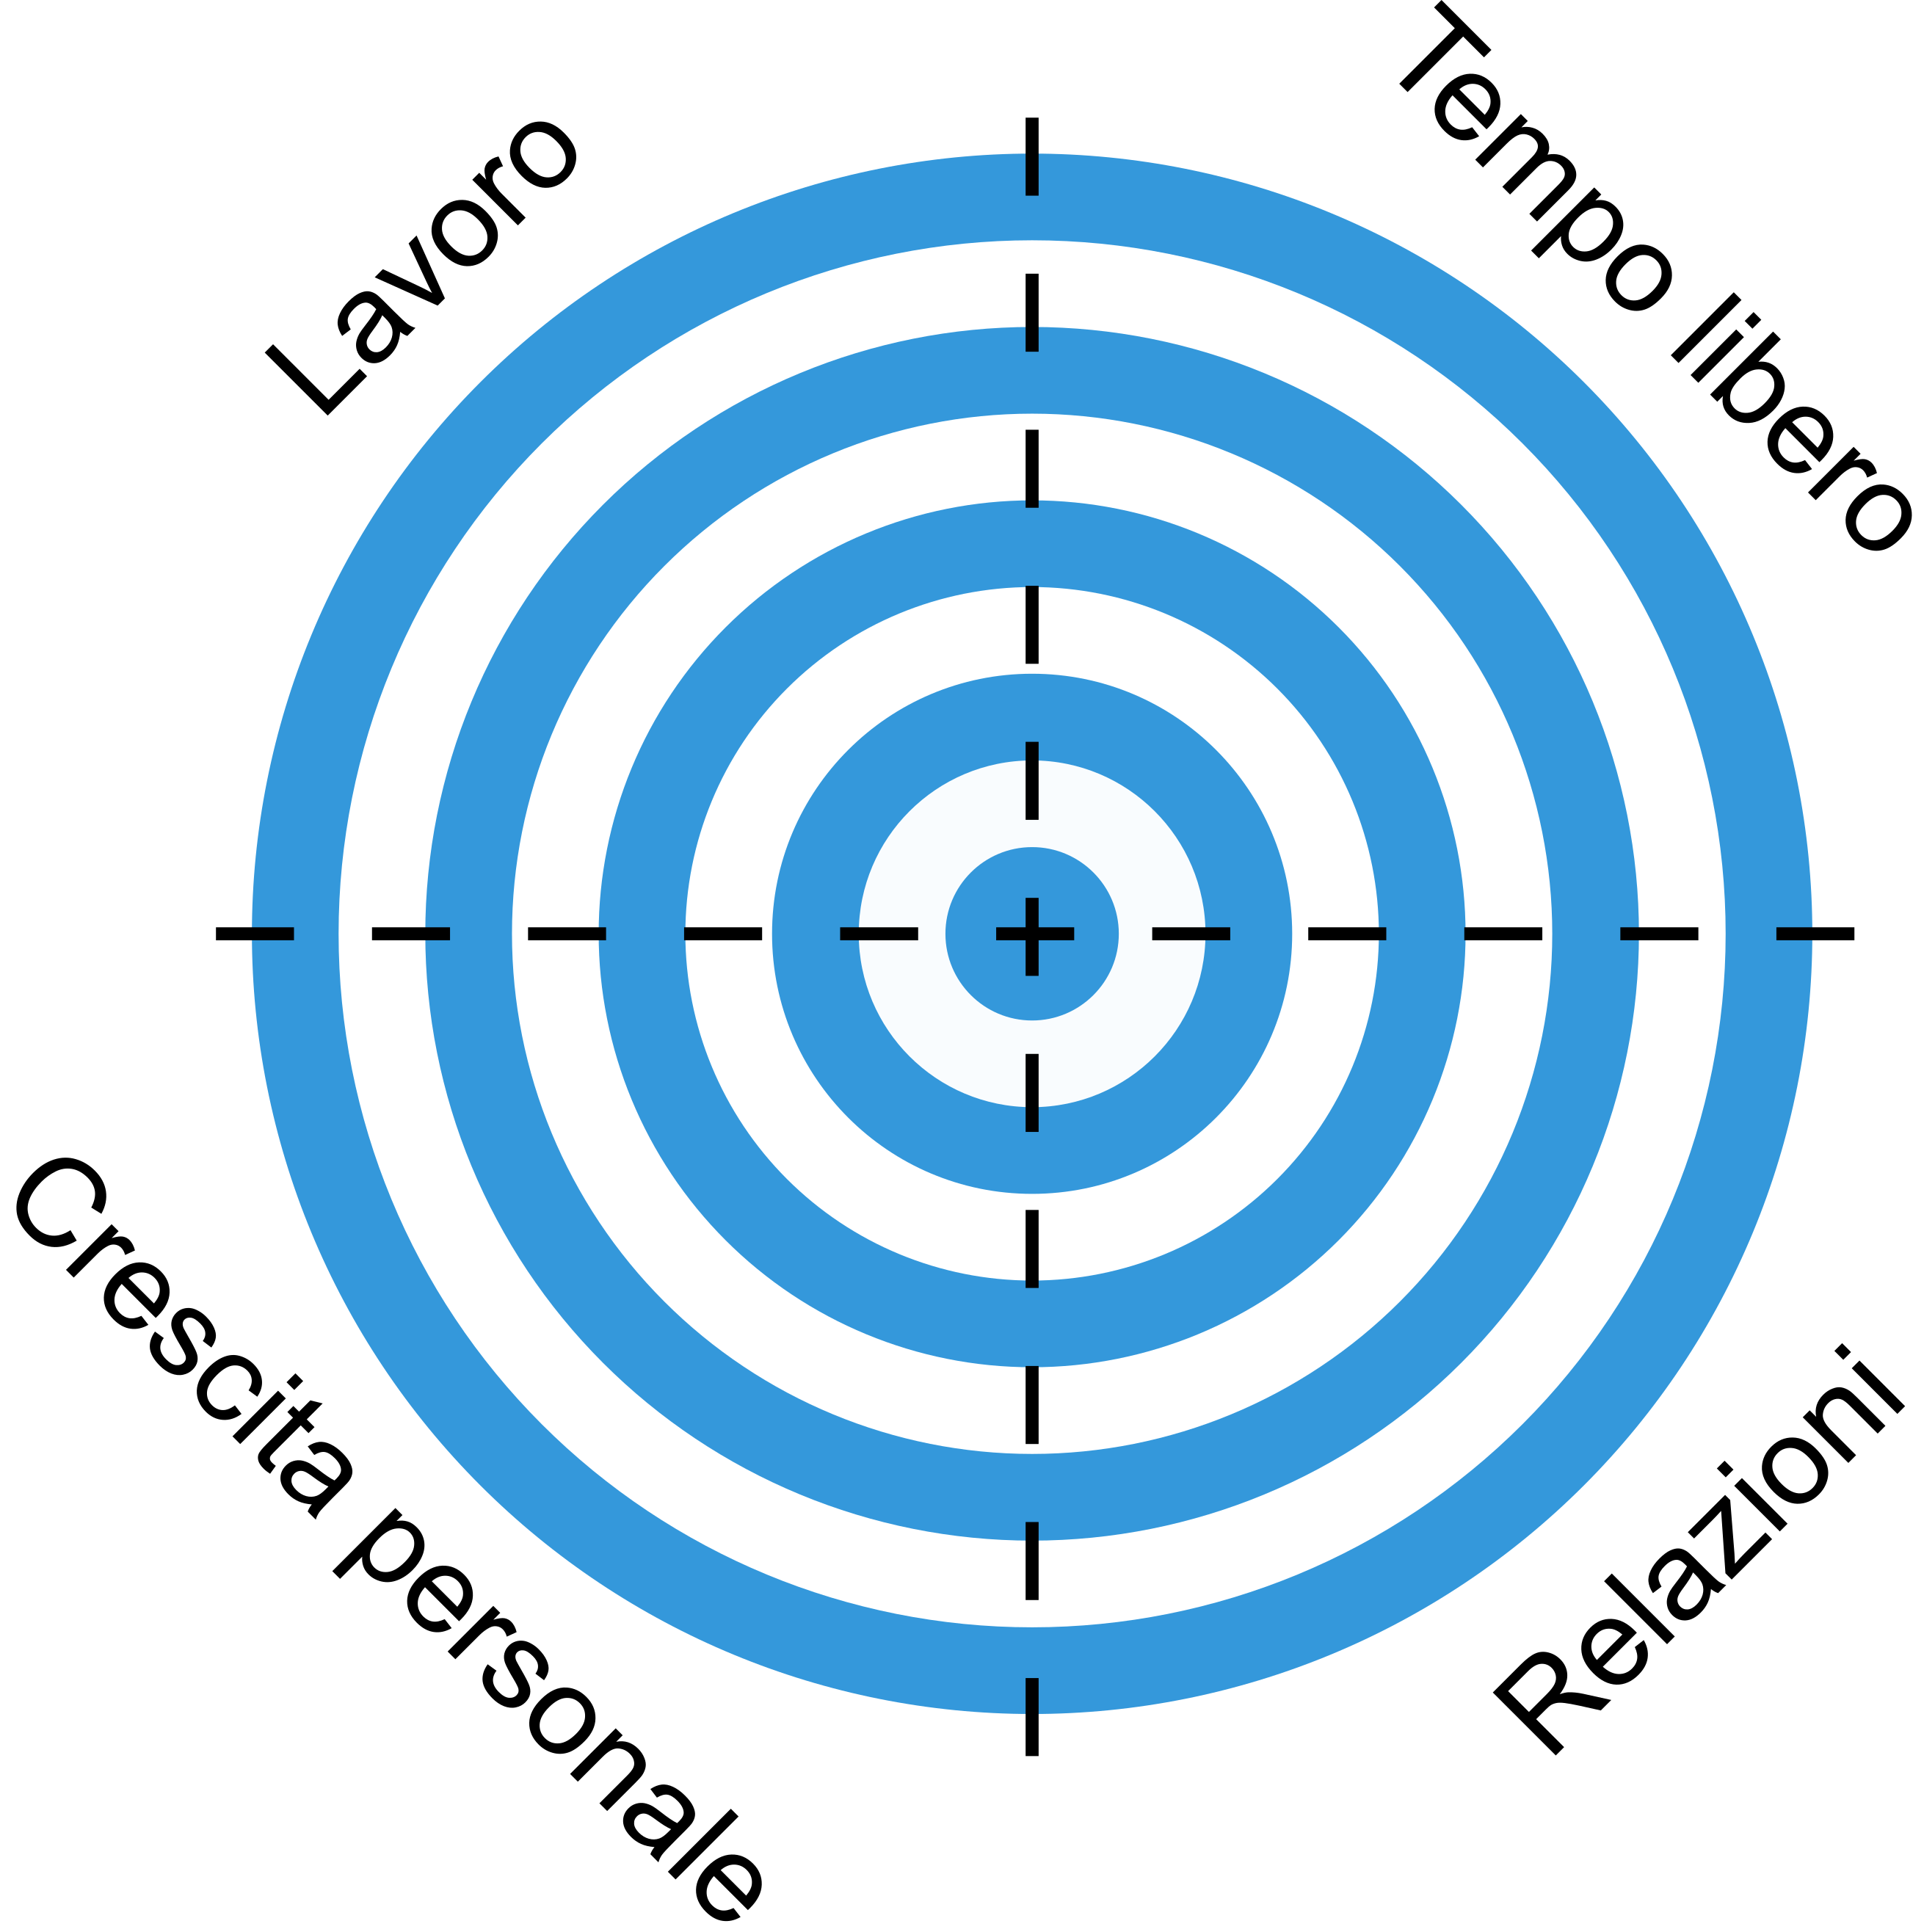
\includegraphics[width=0.95\linewidth]{images/Libro-img014.png}
\end{wrapfigure}

Possiamo fare anche un lavoro che non ci piace e, farlo con piacere se riusciamo a portarci dentro i nostri valori, se
riusciamo a farlo in linea coi nostri valori. I valori giustificano la fatica perché ne vediamo il senso. Se tra i
nostri valori c'è l'ambiente per noi varrà la pena faticare per avere uno
stile di vita più sostenibile. Se nei nostri valori c'è la famiglia, per noi varrà la pena
dedicare del tempo a giocare coi figli. Se nei nostri valori c'è la salute, per noi varrà la pena
lo sforzo di una regolare attività fisica. Potresti chiederti: se non facessi/sentissi/pensassi più in un certo modo, come impiegherei il mio tempo? Se potessi premere un pulsante che mi darebbe la piena approvazione di
tutte le persone che per me contano, quindi, non cercando di impressionare o compiacere nessuno, cosa farei della
mia vita e, che tipo di persona vorrei essere? Altre volte potremmo chiederci: “Ma i miei valori sono in
contraddizione tra loro”. Può capitare di avere valori che vadano in direzioni diverse, ma non lasciare che questo ti
impedisca di agire, si tratta solo di trovare un compromesso o concentrarsi più su un valore rispetto a un altro, dando
quindi una priorità più alta.

A volte sentiamo che bisogna fare quello che si sente, in maniera spontanea, ed è vero! Ma non basta! Questo pensiero,
presuppone erroneamente che tutti gli uomini agiscano in maniera coerente con i propri valori, ma se così fosse sapremmo
già tutti cosa fare per essere felici e lo faremmo. Il nostro cervello tende a essere più sensibile ai pericoli e alle minacce che alle emozioni positive, per ragioni evolutive. Per questo motivo, coltivare la felicità può richiedere intenzionalità e direzione. Senza regole rischiamo di essere preda delle passioni, dei desideri insaziabili, finito uno ne inizia un altro all'infinito. Inoltre, alcune scelte che rappresentano
uno sforzo o qualcosa che non vorremmo fare, possono rivelarsi utili per il futuro, che presto o tardi verrà e ne
potremmo giovare. Una volta che avremo coltivato un maggiore equilibrio interiore e una direzione chiara, potrà emergere un maggiore spazio per la spontaneità.

Concentrati sul significato che dai alla tue azioni e, non sulla felicità. Non chiederti cosa ti faccia felice, ma cosa
fornisca senso alla tua vita.
Se cerchi un significato, quest'ultimo lo potrai trovare sia nei momenti felici che in quelli tristi. Nei momenti tristi chiediamoci: qual è il significato di questo momento? A cosa mi servirà sopportare certe fatiche?
Quando ci fissiamo rigidamente sull’idea di dover essere sempre felici, rischiamo di reagire con evitamento o disagio ai momenti di difficoltà, perdendo l’opportunità di dargli un senso.
Se invece cerchi un senso, anche nella tristezza, non sarai frenetico nell'attesa che questo momento passi, perché anche quel momento potrebbe acquisire un suo significato.

\begin{mdframed}[linewidth=1pt]
Motivazione Vs Metodo

Lo studio di Cheung et al. (2014) suggerisce che la differenza tra individui con alto o basso autocontrollo è in gran parte dovuta alle strategie adottate per raggiungere gli obiettivi piuttosto che al tentativo di sopprimere gli impulsi. Il benessere è legato in un certo modo a delle regole, a mettere in atto strategie funzionali e comportamenti desiderati, adottando approcci che, pur mirando a obiettivi a lungo termine, non escludano la possibilità di godere dei piaceri momentanei. Ma come
riuscirci in un mondo pieno di tentazioni o quando i nostri obiettivi confliggono tra loro? 

Quando riusciamo ad avere delle routine o delle buone abitudini diventiamo in grado di mettere in atto comportamenti
desiderati con meno sforzo in quanto automatiche. Il perseguimento di un obiettivo risulta quindi facilitato
dalla messa in atto di abitudini, piuttosto che dalla soppressione degli impulsi indesiderati, che potrebbero prosciugare le
risorse di autocontrollo rischiando il fallimento, lasciandoci quindi più energie per le nostre
attività\endnote{\raggedright\url{https://www.stateofmind.it/2021/05/autocontrollo-impulsi/} }. Anche il prendersi delle pause, seppur
sia vista come una cosa opposta alla produttività, possono invece ridarci nuove energie e farci ritornare più motivati,
se fatte entra una certa misura. In Diventa chi sei\endnote{\raggedright\url{https://www.amazon.it/dp/B079TLH7PK} }, Emilie Wapnick
consiglia 40 minuti, ma possono essere di più o di meno a seconda della persona. Un altro consiglio per trovare la
motivazione è: iniziare!
Uno studio\endnote{\raggedright\url{https://www.sleepfoundation.org/sleep-hygiene/coffee-nap}} ha confermato che un breve pisolino di 15-20 minuti può essere più efficace del caffè per aumentare l’energia e la concentrazione.
Lo studio “Close, and ye shall find: eye closure during thinking enhances creativity”\endnote{\raggedright\url{https://www.nature.com/articles/s41599-018-0138-0.pdf}} suggerisce che chiudere gli occhi per due minuti durante il pensiero può stimolare la generazione di idee più creative e flessibili.

Frasi come: trova il lavoro che ami e non lavorerai nemmeno un giorno, non sono del tutto vere in quanto la scintilla,
la musa, la voglia, la motivazione, arrivano e si esauriscono, quello che resta poi è l'essere organizzati,
disciplinati e lavorare. Anche godersi il processo o il viaggio invece del traguardo, va preso in maniera relativa.
Questo perché è improbabile che ci piaceranno tutte le cose del processo e, se dovessimo mettere in dubbio la scelta
del nostro viaggio perché non ci sta piacendo tutto, dall'inizio alla fine, rischiamo di mettere le basi per la nostra insoddisfazione. Come al solito uno sguardo va alle aspettative perché possono frenate la
motivazione. Se io mi dico: devo arrivare la, ottenere quella cosa entro X tempo, potrei non farcela, perché ci sono
fattori indipendenti dal mio agire che possono interferire e demotivarmi, facendoci sentire non all'altezza.

Non esiste una formula che vada bene per tutti. Per qualcuno l'ideale è trasformare la propria
passione in lavoro, mentre per altri è fare un lavoro remunerativo o che lasci abbastanza tempo libero proprio per
poter coltivare le proprie passioni fuori dal lavoro.

Altre volte siamo demotivati perché non riusciamo a completare le cose che ci siamo prefissati. Come spiega Chris
Guillebeau, “[noi] sopravvalutiamo quello che possiamo realizzare in un solo giorno, ma sottovalutiamo quello che
possiamo fare in un anno”. Non hai bisogno della motivazione per fare le cose ma di metodo. Spesso dimentichiamo che la
parola Motivazione è formata da motivo e azione. Un invito all'azione. La passione è molto forte all'inizio ma col tempo potrebbe diminuire e allora
non sarà più quest'ultima a farci muovere ma un metodo, una struttura.

Sulla motivazione ci sono due teorie: 
Dire a tutti dei tuoi obiettivi, così sarai spronato per mantenere la coerenza davanti ai loro occhi.
L'altra teoria invece dice di non dirlo in giro, per evitare che la gente ti demotivi. Queste teorie sono vere entrambe, l'ideale è usare un mix di queste due tecniche e dire i propri obiettivi solo alle persone vicine a noi che sappiamo che non ci feriranno.
Anche le teorie tipo fake it until you make it, ovvero, fai finta finché non diventa vero, possono talvolta funzionare aumentando la fiducia, ma in altri casi possono portare a una falsa percezione di aver già raggiunto il traguardo, riducendo la motivazione ad agire.

Scott Adams dice che per aver successo o sei il migliore di tutti a fare una certa cosa, ma è quasi impossibile, o hai
un set di due o più abilità in cui sei nel gruppo dei 25\% dei più bravi, così da creare una competenza molto specifica
in cui sei tra i migliori. La maggioranza della gente ha come passioni arte e sport, attività difficilmente
convertibili in lavoro, per questo non dovremmo sentirci inadeguati se non riuscissimo a convertire le nostre passioni
in un lavoro.

Secondo Robert J. Vallerand, la passione ha due principali connotazioni: armoniosa o ossessiva. Quelli che provano una
passione armoniosa si impegnano nel lavoro perché ne traggono una gioia intrinseca, e la loro professione convive in
armonia con le altre attività della loro vita. Al contrario, con la passione ossessiva, si ha
un'incontrollabile urgenza di lavorare vivendo in maniera conflittuale la passione e le altre
attività presenti nella loro vita.

La necessità di un lavoro che assecondi le proprie passioni come requisito di una vita ben spesa potrebbe essere un bisogno nato dalla
generazione Y, ovvero quella nata tra gli anni 80 e 2000. Questa ricerca sembra aver portato più stress e
insoddisfazione rispetto alle generazioni precedenti che sceglievano un qualsiasi lavoro potesse dar loro stabilità
economica. Con questo non voglio dire che un lavoro in linea con le nostre passioni sia da evitare, al contrario, ma se la ricerca o il lavoro vengono vissuti in maniera ossessiva, potrebbe essere più salutare un approccio di accettazione, anche di un lavoro meno appagante, piuttosto che persistere in una dinamica distruttiva. A volte non aver scelta dona più libertà.

Per alcune persone è più funzionale dedicare tutta la vita a un progetto, per persone multipotenziali no. Passare da un tema
all'alto, in maniera lenta, dandosi il tempo di approfondire un argomento finché suscita interesse
in noi, che può durare anni, si chiama slow motion multitasking (in quanto il multitasking simultaneo nello stesso
momento, non esiste). Questo saltellare da un tema all'altro, verrebbe visto negativamente, come
una persona con le idee poco chiare. Ma questo ha diversi vantaggi, oltre all'annoiarsi meno,
quello che si apprende in una materia lo si può portare nella risoluzione di problemi in ambiti completamente diversi
e, questa contaminazione, si può anche chiamare in un altro modo:
creatività\endnote{\raggedright\url{https://www.youtube.com/watch?v=O3YFD9T7fTc} }.

Solitamente viene malvisto lasciare a metà le cose e saltare da un progetto all'altro. Ma dipende
qual è l'obiettivo. Spesso per i multipotenziali l'obiettivo è imparare
qualcosa, quindi quando questo viene raggiunto si passa a qualcos'altro anche se la parte pratica
non è stata ultimata. Sembra che queste persone mollino quando l'attività diventa troppo
complicata, al contrario, questo avviene quando quest'ultima non ha più nulla di stimolante da
offrire. Bisogna stare attenti però a non darsi questa scusa per giustificare la scarsa concentrazione.

Routine, abitudini e creatività non sono infatti in contraddizione. Come diceva Kobe Bryant la creatività ha origine
dalla struttura. Quando hai certi parametri e una struttura, puoi essere creativo al loro interno. Se non hai struttura
rischi di fare solo cose a vanvera. Per fare un discorso, ad esempio, difficilmente sarai spontaneo. Se lo prepari bene, puoi usare quello come punto di partenza per fare delle variazioni ed essere spontaneo. Regole e routine alleggeriscono il fardello cognitivo garantendoci lo spazio mentale
necessario alla creatività.

Se non sei pronto rischi di muoverti a caso, facendo confusione e penserai solo a sistemare il problema rendendoti difficile la spontaneità.

Anche nella coppia, le abitudini sono spesso demonizzate. Raffaele Morelli racconta di
questa donna sposata che è a conoscenza dell'amante di suo marito. La donna racconta che da
qualche anno, anche lei ha trovato un amante con cui c'è molta passione. Dopo tre anni l'amante di lei le
chiede di diventare la sua compagna e lasciare il marito. La donna però ha preferito continuare a stare con il suo
marito e, si sentiva in colpa di questa decisione, di aver rifiutato l'amante con cui andava tutto
bene, per restare nella vecchia relazione fatta di silenzi. Secondo Morelli invece questa non è una scelta sbagliata,
perché nessuna scelta lo è per la psiche. Se hai fatto quella scelta è perché in quel momento, per la tua crescita, per
la tua maturazione, avevi bisogno di fare quella scelta, poi dal punto di vista pratico, col senno di poi potrebbe
risultare positiva o negativa, ma per la tua psiche era necessaria e giusta proprio quella che hai fatto, eventualmente
per non ripeterla più. Se potessimo tornare indietro nel
passato, con le stesse conoscenze, nella stessa situazione, nello stesso ambiente, faremo probabilmente le stesse scelte.
La passione non è fatta per durare, mentre le abitudini si. Questa dinamica può aver influenzato la scelta della signora del racconto.
Il suo disagio, ancora una volta, non era legato all'evento in sé, ma al giudizio che è stato dato.

Un altro esempio è la pigrizia. Secondo i ricercatori della Ohio State University analizzando gruppi di studenti che si
rilassavano su un divano, hanno osservato che i partecipanti che pensavano fosse sbagliato impiegare il tempo senza
"produrre" si godevano meno il relax . Al contrario l'idea cambiava se
si pensava che l'attività svolta nel tempo libero potesse portare ad un beneficio a lungo termine. Non è sbagliata
l'attività in sé, ma piuttosto il pensare che sia tempo sprecato è dannoso per la salute. La sensazione
di sprecare il tempo, ci dice qualcosa di fondamentale su di noi, non ci dice qualcosa sulla realtà. Forse non stiamo
vivendo in linea coi nostri valori o forse il nostro giudice interno è troppo esigente. Semplicemente possiamo notarlo. Non
fare niente non è mai fare niente: ti obbliga a riflettere e a compiere libere associazioni, che si possono rivelare
utili. Gennaro Romagnoli nella puntata 81 consiglia di allenarsi a non fare niente, per non avere il pilota automatico sempre sul "fare".
\end{mdframed}

In psicologia si osserva spesso una relazione bidirezionale tra autostima e azione: se non agiamo, falliamo, e questo può abbassare l’autostima; viceversa, una bassa autostima può ostacolare l’azione. Quindi l'autostima può essere l'effetto, non la causa e, questo può essere osservato in diverse abilità psicologiche.

Il nostro benessere e la nostra felicità dipendono da come interpretiamo la realtà, che significato e definizione gli
diamo e quali aspettative avevamo a riguardo. Noi non possiamo vedere la realtà, ma solo interpretarla e probabilmente deformandola. Studi sulla psicologia del linguaggio suggeriscono che il framing linguistico può influenzare le emozioni e la percezione: esprimersi con parole diverse può modellare il nostro stato emotivo.

Persone che parlano in modo diverso della stessa cosa, vivono in modo diverso e la realtà per loro è diversa. c'è
differenza infatti tra dire:\newline
“che freddo” o “si congela”\newline
“ho mal di testa” o “mi scoppia la testa”\newline
“sono stanco” o “sono distrutto”\newline
“mi urti” o “mi fai uscire di matto”

Le parole ci suggestionano. Se diciamo “non ho mai tempo” difficilmente riusciremo a introdurre qualcosa di nuovo nella nostra vita.
Se siamo abituati a dire spesso “sono stanco”, tenderemo a sentirci stanchi davvero. Con questo non vorrei che passasse l'idea che se mi ripeto una cosa diventa realtà, altrimenti basterebbe dire: sono pieno di energie! Riuscendoci a concentrare solo su una cosa per volta, se ci concentriamo solo sulla stanchezza, nella nostra esperienza interna, esisterà solo questo, se ricordiamo solo i momenti della giornata in cui eravamo impegnati e non quelli dove stavamo sui social, potremmo pensare di non avere mai tempo e così via. Se diciamo agli altri: “sei pallido…” o “ti senti bene?” potrebbe portare le persone a indagare dentro di sé la presenza di problemi e spesso qualcosina si riuscirà a trovare e a ingigantirla, quindi se chiedo a qualcuno: "sei arrabbiato", anche se prima non lo era, potrebbe diventarlo. Per questo fare una cosa alla volta è un modo straordinario di meditare e di restare consapevoli.

Altro esempio, dire: “non sono capace” porta con se una giudizio, un limite, che porta alla “profezia che si
auto-avvera” rendendoti davvero incapace di compiere quella cosa. Mentre dire “non sono ancora capace” da una
potenzialità completamente diversa all'atto che stai per compiere. Alcuni studi (es. Rosenthal, 1968) evidenziano che le profezie che si auto-avverano tendono a essere più forti nei contesti negativi, dove le aspettative limitanti influenzano il comportamento, quindi ha molto più effetto quando ci scoraggiamo rispetto a quando ci incoraggiamo. Il pensiero positivo volontario può risultare paradossalmente controproducente se non supportato da strategie realistiche: l’effetto placebo funziona meglio quando le suggestioni sono inconsce, non imposte consciamente. Quando utilizziamo
volontariamente il pensiero positivo, avviene un effetto paradossale, ovvero: Se sono triste e mi sforzo di pensare
positivo, la sensazione resterà ma, non essendo in linea con il pensiero, la mente vedrà questo come un problema e,
come sappiamo, il compito del cervello è risolvere i problemi. Questo ci portebbe portare a chiederci cosa
c'è di sbagliato in noi, cosa dovremmo cambiare e altre domande potenzialmente disfunzionali. Il
pensiero positivo, che all'apparenza sembra una buona idea, può portare all'effetto
opposto, peggiorando lo stato d'animo. Pensare ai propri disagi è sempre sbagliato? La tristezza può arrivare per portarci a cambiare qualcosa, altre
volte invece va tutto bene, ma possono essere le nostre domande a farci diventare tristi, soprattutto quando ci concentriamo su
quello che non abbiamo e che magari è un desiderio indotto dall'esterno.

La “positività tossica” si riferisce alla convinzione che si debba mantenere un atteggiamento positivo e ottimista in ogni situazione, ignorando o svalutando le emozioni negative. Uno studio condotto dalla Tilburg University\endnote{Perceiving societal pressure to be happy is linked to poor well-being, especially in happy nations \raggedright\url{https://www.nature.com/articles/s41598-021-04262-z}} nei Paesi Bassi, che ha coinvolto circa 7.443 persone provenienti da 40 diversi paesi, ha esaminato l’impatto della pressione sociale per la felicità sul benessere individuale.
Il paradosso scoperto è che l’incoraggiamento sociale a mantenere un atteggiamento positivo può avere effetti negativi, portando talvolta a esperienze di emozioni positive meno frequenti e meno intense, mentre potrebbe intensificare quelle negative. Questo studio che ha coinvolto soprattutto in paesi con alto indice di felicità, mostra una correlazionee e non causalità. L’idea di dover essere costantemente felici, che è irrealistica, può far sentire le persone inadeguate e l’atto di reprimere le emozioni negative può paradossalmente intensificarle.

Ellen Langer ha condotto un esperimento con degli anziani. La ricercatrice ha condotto diverse misurazioni sulla
pressione sanguigna, ossigenazione del sangue, frequenza respiratoria, livelli di attenzione, ansia, benessere ecc…
poi li ha portati in un villaggio a tema anni 60 e, ha chiesto loro di parlare al presente, come se fossero davvero gli
anni 60, con i modi di dire, le situazioni, vestiti, insomma comportandosi e facendo tutto come se fossero ritornati
indietro nel tempo. Dopo un periodo ha ricondotto le misurazioni sugli anziani e ha notato un miglioramento generale.
Alcuni di loro, privi di qualsiasi potere decisionale sulla propria vita, non avevano nemmeno il controllo su ciò che
mangiavano. Tuttavia, una volta che è stata loro concessa la possibilità di prendere decisioni su alcuni aspetti della
propria esistenza, si è notato un ulteriore ringiovanimento nelle misurazioni. Tuttavia va precisato che lo studio era piccolo e senza un controllo rigoroso, quindi richiede ulteriori repliche.

Pensate alla differenza, in una conversazione, di queste due espressioni: “non hai capito” o “mi sono spiegato male”.
Nella prima forma una persona suppone di essersi spiegata bene e che il problema sia l'altro, ma non ne ha nessuna
certezza, mentre nel secondo caso, si mette in dubbio la propria esposizione invece della comprensione dell'altro.

In realtà le cose, la vita, le persone sono quello che sono ma il modo in cui noi le definiamo può influenzare significativamente la nostra esperienza, come mostrano gli studi sul framing e la percezione interpretativa. Abbiamo visto sia irrealizzabile cercare in una relazione di coppia, anche dopo molti anni, le
emozioni dei primi mesi. Ma se noi definiamo come “amore” i sentimenti dei primi tempi, potremmo interrogarci sul fatto
che non amiamo più. Se dopo diverse relazioni ci troviamo a fare sempre la stessa domanda potremmo arrivare a
interrogarci sul fatto di non essere in grado di provare amore. O la “felicità”. Se trovo la felicità potrei sperimentare paura dal perdere le condizioni che mi ci hanno portato. Se pensiamo che una volta ottenuta la stabilità economica, una
compagna o un compagno, un lavoro, famiglia e figli otterremo una felicità perpetua, immutabile, senza più provare
tristezza, ecco che stiamo dando alla felicità un significato irrealizzabile. Ma noi potremmo continuare a cercare quella
felicità impossibile che ci causa frustrazione. Noi possiamo diventare tristi appena pensiamo di essere tristi, anche se magari non lo
siamo veramente. Possiamo sperimentare tristezza appena nascono pensieri tristi e il nostro dialogo interiore continua a parlare di
questa tristezza, alimentandola. Gli studi sul coping emotivo, ad esempio quelli di Nolen‑Hoeksema, suggeriscono che la ruminazione continua può intensificare e prolungare stati emotivi come la tristezza.

Non siete sbagliati voi, gli altri, la vita, le circostanze, semplicemente in quel momento, vi sentite così, ne prendete
atto e lo accettate, consapevoli che tutto passa e che potreste sentirvi tristi della tristezza, aver paura della
paura, più che della tristezza o della paura in sè. Spesso siamo afflitti per il giudizio che queste cose non dovrebbero
andare così, per la definizione che abbiamo dato di come dovrebbero andare le cose. 

La felicità dipende anche da aspetti legati alla cultura ed al posto in cui viviamo. In Nordamerica la felicità viene
definita con la realizzazione personale (compreso il piacere), mentre in Asia orientale la felicità è generalmente associata
all'armonia sociale. 
Essere felici in una determinata cultura dipende tanto da quanto le vostre emozioni sono sincronizzate con la
definizione di felicità espressa in quel contesto sociale. 
Su quale principio ci sentiamo in dovere di essere sempre allegri?

Quando il saggio indica la luna lo stolto vede solo il dito (proverbio cinese). 

Trovare continuamente difetti sul proprio aspetto fisico, per esempio dire delle proprie mani: “sembrano quelle di un
vecchio” oppure dire “sono con me da tutta la vita e grazie a loro ho fatto un sacco di cose” farà vivere queste due
persone in una maniera diversa. Questo può succedere per tutto, il lavoro, il meteo, i suoceri, genitori,
figli. Il Wabi-sabi, filosofia estetica giapponese, da cui deriva l'arte di riparare i vasi rotti evidenziando le crepe con dell'oro,
cerca di vedere il bello nelle imperfezioni, apprezzare il tempo che passa, le
rughe e la saggezza. Pensando al tempo che passa, non portiamo l'attenzione su ciò che abbiamo perduto, ma alla gratitudine di ciò che abbiamo conquistato.

Sulla relazione con gli altri e con noi stessi è giusto essere critici verso i comportamenti, distinguendoli il più possibile verso la persona tra cui noi stessi. 
Possiamo additare un pedofilo, un assassino
come un mostro e poi scoprire che per anni, nell'innocenza di bambino che è stato, senza colpe, ha
subito le peggiori violenze. Comprendere queste origini non attenua la gravità delle loro azioni, ma ci invita a riflettere sulla complessità del comportamento umano. Nei giusti contesti anche noi potremmo diventare dei mostri come abbiamo visto
nell'esperimento del carcere di Stanford, seppur presenti limiti metodologici e non testimoni cambiamenti individuali inevitabili.
Se siamo persone che hanno la tendenza a criticare gli altri
probabilmente critichiamo anche noi stessi. Non dovremmo etichettare negativamente o come insicuro chi cerca i
plausi, ma riconoscere che tutti noi abbiamo queste tendenze umane in modalità diverse. Questo della sicurezza è solo
un esempio, pensiamo ad ogni critica e notiamo come possiamo applicare questo ragionamento.

Quando giudichiamo qualcosa lo definiamo. La parola definire deriva dal latino e significa limitare, stabilire dei
confini. Quando noi definiamo qualcosa o qualcuno stiamo stabilendo delle regole sui suoi confini, stiamo limitando ciò
che è o può essere. In altre parole, stiamo confinando qualcuno o qualcosa in una definizione molto stretta che può diventare una 
trappola sia per noi che per l'altro, svilendo e appiattendo il lavoro di crescita personale che questo individuo può aver fatto.
Può avvenire in maniera più esplicita con il razzismo o in modo più velato con il segno zodiacale.

Quando definiamo una persona, in qualche modo, dentro di noi, ci siamo messi dalla parte del giudice, ed emesso
una sentenza, una condannata a delle conseguenze. 
A volte siamo molto bravi a creare delle trappole da cui gli altri o noi stessi fatichiamo ad uscire.
Ad esempio, se accuso qualcuno di narcisismo, la persona, nel tentativo di giustificarsi, potrebbe focalizzarsi su se stessa, alimentando involontariamente l'accusa. O ancora, se dico che sei permaloso con insistenza, una reazione di rabbia potrebbe essere interpretata come una conferma dell'accusa, creando una situazione difficile per l'accusato.
Noi siamo quello che siamo,
indipendentemente dai giudizi, ma definendoci faremo più fatica ad esserlo. Per questo ogni tanto ci
sentiamo inadeguati verso certe situazioni, verso noi stessi, verso gli altri o i sentimenti. O meglio, ci sentiamo inadeguati verso il giudizio, la sentenza, la definizione che abbiamo dato a tutte queste cose, che spesso sono basate su standard irrealistici o idealizzati.

Prendiamo un esempio più ambiguo:
una persona che arriva in ritardo. Noi ci diciamo che è una mancanza di rispetto per
il nostro tempo, perché noi siamo arrivati puntuali e siamo stati costretti ad aspettare, senza poter fare niente,
annoiandoci, se avessimo saputo che ci fosse stato questo ritardo potevamo stare a casa a finire di fare alcune commissioni.
Questa persona però non ci ha messo delle catene, noi potremmo mandare un messaggio e
scrivere: Troviamoci in libreria, così intanto guardo se è uscito quel libro che cercavo, o altrimenti, io entro al
cinema, così non mi perdo l'inizio e te lo racconto, ecc… Quindi perché rimaniamo lì ad aspettare,
immobili, pieni di pensieri su come tutto questo sia sbagliato? Perché se abbiamo una scelta non facciamo niente?
Perché le nostre definizioni ci dicono che, primo, si arriva all'orario prefissato e secondo, si
aspetta nel punto prestabilito. Non abbiamo delle catene fisiche, ma catene mentali, anche se il risultato può essere lo
stesso. Con questo non voglio dire che sia giusto arrivare in ritardo, ma dico che se potessimo entrare nella testa
della persona, probabilmente lei voleva arrivare in orario, non voleva farci rimanere
male, ma purtroppo non c'è riuscita e magari non ci riesce molto spesso. Troviamo studi anche su questo e ci sono diverse motivazioni. Tra le teorie più diffuse sembra che alcune persone non abbiano una
buona memoria temporale e percepiscono lo scorrere del tempo in maniera diversa. Ad esempio, quando si
preparano, o fanno il tragitto in auto, se impiegano venti minuti, hanno la percezione di averci messo meno tempo, portandole a sottostimare i tempi, rischiando di farle arrivare in ritardo. Se sappiamo che
non era intenzione della persona farci stare male, avremmo ancora buone ragioni per avercela con lei?

Ora io ho fatto l'esempio del ritardo, ma se ne potrebbero fare tantissimi altri. Per trovare
l'esempio giusto per voi, ripensate a tutte le volte in cui avete subito un'ingiustizia o
che qualcuno si sia comportato male con voi. Ora però provate a
cercare le motivazioni che hanno portato quella persona a fare quella cosa, è possibile che non troverete il volervi
ferire.

Quando sentiamo un giudizio possiamo vederla come la mente che ci sta
dando dei suggerimenti (non delle condanne), prendiamo in considerazione quello che ci dice in un secondo momento, ora torniamo a fare quello che stavamo facendo e poi lo valuteremo.

Se ci sentiamo
sbagliati e secondo noi, secondo il nostro giudizio, dovremmo cambiare. Non è consigliabile forzare se stessi e farsi
violenza, possiamo cercare di essere ciò che siamo e eventualmente cambiare coi giusti tempi. La mindfulness e la
meditazione non hanno il fine di cambiare le cose ma si limita ad osservarlo, senza intervenire, accettando senza giudicare i
propri lati di sé, anche quelli che ci piacciono meno. Questo non vuol dire sedersi sulle proprie cattive abitudini
giustificandosi dietro la frase “sono fatto così, non ci posso fare niente”. Se riconosciamo di avere un certo lato
di noi, accettandone l'esistenza, aumentiamo le probabilità di diventarne consapevoli, che è una delle vie più efficaci per gestire questo lato prima di agirlo.

Se hai poca autostima forse no sarai contento ma se ne hai molta, potrebbe portare ad uno sforzo continuo per paura di perderla. Come
sarebbe la tua vita senza autostima e i relativi giudizi di come dovresti essere? Questa idea non basterà a bloccare la
tua mente dall'emettere giudizi, ma potresti iniziare a vederli per ciò che sono, semplici pensieri.
Quindi, la prossima volta, tra pochi secondi, che etichetterai qualcosa o qualcuno con qualche definizione, non fare
niente. Semplicemente annotalo, osservalo, prendine atto, sii
testimone\endnote{\raggedright\url{https://www.maxfuria.com/le-parole-che-ti-cambiano-la-vita-e-quelle-che-la-peggiorano/}}
\endnote{\raggedright\url{https://amico-in-affitto.com/2017/08/14/le-parole-che-cambiano-la-vita/}}.

\begin{mdframed}[linewidth=1pt]
Nel libro l'illusione della memoria\endnote{\raggedright\url{https://www.amazon.it/dp/8868334313} } di Julia Shaw abbiamo numerosi esempi
e spiegazioni di come, il nostro principale oggetto riguardante la nostra identità, sia fallibile. La nostra mente
potrebbe ricordare delle cose mai vissute e tutti facciamo esperienza di questo errore, solo che non possiamo saperlo.
Sembra infatti impossibile avere ricordi avvenuti prima dei nostri 3 anni di età, eppure, la maggior parte degli adulti, potrebbero giurare
di aver delle immagini di quel periodo. Ma com'è possibile? Questa tipologia di memorie si
chiamano ricordi indotti. Probabilmente i nostri genitori ci hanno raccontato di quell'episodio,
magari mostrandoci anche delle foto e, mentre parlavano, la nostra mente ha iniziato a produrre delle immagini. Siccome
quel racconto riguardava noi, l'abbiamo fatto nostro. La memoria infatti non è consultabile direttamente, ma è un processo ricostruttivo del cervello: per accedere a un ricordo tendiamo a ricrearlo mentalmente, un po’ come immaginare una scena. Quando vogliamo accedere ad un ricordo lo possiamo immaginare e, questo processo, spesso deforma anche i nostri veri ricordi. Più
ripensiamo ad un episodio e più rischiamo di deformarlo. Un’esperienza può diventare traumatica in relazione alla percezione soggettiva e alla reazione emotiva; la reinterpretazione può modulare l’impatto. Se una persona vive un trauma e riesce a gestirlo bene, se si confrontasse con altre persone che hanno
vissuto la stessa esperienza e sono in lacrime, questa persona potrebbe rivalutare il giudizio dato all'esperienza. Un
modo per avere ricordi più veritieri potrebbe essere quello di tenere un diario.

La nostra memoria è vittima di numerosi bias. Spesso tendiamo a lasciare nella nostra memoria una traccia
maggiore circa le cose positive che facciamo. Per questo molte persone pensano di essere più brave a guidare rispetto
alla media, o più intelligenti o più attraenti o di fare più faccende domestiche rispetto al nostro partner. I
poliziotti pensano di saper individuare un criminale, un insegnante di essere chiaro nelle spiegazioni e, gli studenti di aver capito tutto. 
L’effetto ‘above average’ o illusione dell’abilità, documentato da Svenson (1981), mostra che molti si vedono sopra la media, ma per ovvie ragioni la metà non potrà esserlo.
Sui ricordi invece, alcune ricerche\endnote{\raggedright\url{https://science.sciencemag.org/content/339/6115/96}} suggeriscono che le persone tendono a sovrastimare gli eventi negativi futuri, ma il fenomeno dipende dal contesto e dalla predisposizione individuale.

Se pensiamo a Steve Jobsh, Mark Zuckerberg e altri, che hanno lasciato l'università e hanno avuto successo, possiamo pensare di farlo
anche noi, ignorando a quante persone invece è andata male. Stesso discorso vale per gli investimenti economici. Quando
ci si trova davanti a qualcosa di miracoloso, per la nostra salute fisica, mentale, finanziaria potremmo essere
entusiasti finché non consideriamo chi invece ha fallito. Quando mi è stato proposto qualcosa di rivoluzionario sono sempre rimasto molto deluso e, ha senso, altrimenti l'avrebbero già fatto in molti.

Queste nuove scoperte hanno cambiato alcuni approcci come quello dell'ipnosi, utilizzata per accedere a ricordi rimossi.
Oggi si teme che possa invece generare nuovi falsi ricordi. 
Anche nella psicoanalisi, se il terapeuta ti fa immaginare un ricordo traumatico potrebbe creare una falsa memoria. Anche certe modalità di interrogatorio, possono addirittura portare una persona innocente a credere di
aver commesso anche cose gravi, come un omicidio o uno stupro. Esami del DNA hanno infatti smentito numerosi confessioni di testimoni oculari.

Julia Shaw spiega come la generazione di ricordi richieda attenzione, quindi l'autosuggestione
passiva o ascoltare audio mentre si dorme per rendere lo studio meno faticoso, si dimostrano strategie poco efficaci.
Anche i giochi per migliorare la memoria sembrano avere un impatto limitato. La ricercatrice spiega anche come la percezione del
tempo sia influenzata dalla memoria. Se abbiamo tanti ricordi di un certo periodo, la percezione che abbiamo è più
lunga rispetto a quando abbiamo pochi ricordi. Secondo l’effetto reminiscenza, la maggior parte dei nostri ricordi autobiografici si forma tra i 10 e i 30 anni, con un picco nell’adolescenza/giovane età adulta (Rubin et al., 1998); dopo il tempo soggettivamente scorre più veloce perché ci sono meno nuovi ricordi.
Nota che quando ti focalizzi le cose durano di più… Quindi se vuoi massimizzare un momento piacevole, potresti prestarci maggiore attenzione.
\end{mdframed}

Concludo dicendo che il giudizio non è il male. Il giudizio è necessario per valutare e prendere decisioni. Seriusciamo ad accorgerci di ub giudizio possiamo chiederci: quale bisogno ci sta dietro?
Perché abbiamo sentito il bisogno di dare questo giudizio? Mentre invece è molto utile il giudizio, quando siamo noi a
volerlo, in maniera consapevole.
Nulla è sbagliato in assoluto, anche il mind wandering, ovvero quando la mente inizia a vagare. Possiamo darci degli spazi, ad
esempio quando siamo sotto la doccia, per lasciare vagabondare la mente, ma allo stesso tempo possiamo invece scegliere
di essere presenti alle nostre sensazioni, non esiste un giusto o uno sbagliato. Mentre lasciare che la mente vada
nella sua default mode network, ovvero la sua modalità standard, dove è libera di vagare, è poco funzionale quando
stiamo lavorando o in qualsiasi situazione necessiti della nostra presenza mentale o attenzione. 
La default mode network e il mind wandering permettono infatti di essere creativi, non vanno quindi
demonizzati\endnote{\raggedright\url{https://www.psicologianeurolinguistica.net/2016/06/mindwandering-meditazione.html} }.
L'ideale sarebbe riuscire a scegliere noi, grazie alla nostra consapevolezza, in quale modalità
portare la nostra mente, in base al nostro scopo in quel momento.

Non bisogna essere sempre presenti, nemmeno cercare di passare la maggior parte del tempo in questo stato. Se ti viene
voglia di essere più presente, puoi essere più presente. Se vuoi far vagare la mente, puoi far vagare la mente. è come
la palestra. Dovresti fare esercizi tutto il giorno? No! Anche se fa meglio camminare che stare seduti, non è sempre
possibile, né funzionale per ciò che vogliamo diventare. Non vivere l'attimo con ansia. Altrimenti il carpe diem diventa una prigione.

Quando sei felice, facci caso!
Matt Killingsworth di Track yourhappiness.org ha condotto uno studio in cui oltre quindicimila partecipanti
documentavano il proprio stato d'animo e ciò che stavano facendo. Sulla base di oltre 650.000
testimonianze la ricerca ha scoperto che, a prescindere dalle loro attività specifiche, le persone si dichiaravano
significativamente più felici quando erano completamente immerse nel presente. L'effetto non dipendeva da ciò che stavano pensando. Potevano essere impegnate in un pensiero piacevole, neutro o sgradito.
Quand'erano concentrate su elementi esterni al presente erano meno felici. 

\subsubsection{Aspettative}
Ne parlo spesso all'interno del libro. Molto spesso capita che soffriamo perché avevamo delle
aspettative su un certo oggetto, sul futuro, su una persona e poi, quando le cose si sono mostrate diverse da come le avevamo
immaginate, ci soffriamo, anche se, nulla ci avesse dato modo di pensare che sarebbe potuto essere così, ci avevamo
sperato. Va da se che quando abbiamo aspettative su qualcosa, soprattutto sulle persone, spesso possono diventare pretese. È spesso
la nostra mente a preparare il terreno fertile per il nostro malessere.
Ci sta avere delle aspettative, ma bisogna stare attenti a non farle diventare delle pretese. 
Per essere deluso prima ti devi illudere con frasi come: Sarà così per sempre, mi/ti conosco bene, a me non accadrà mai, ecc…

Possiamo chiederci: ogni volta che proponiamo qualcosa a qualcuno, se quest'ultimo dice no, come reagiremo? In base a
questa possiamo capire se si tratta di una aspettativa o una pretesa. Anche qua, non esiste un bianco o un nero, anche
la pretesa non è sempre sbagliata, nel caso ci siano dei patti impliciti o espliciti ad esempio.

Notate che ritroviamo il pensiero dicotomico, o bianco/nero (parole come tutto, niente, mai, sempre, ogni volta ecc..).

Per lo stoicismo, in controtendenza con l'idea comune, il pensiero pessimista diventa un utile
esercizio per la felicità. Più che immaginare che una cosa andrà bene, si ipotizza che una cosa andrà male, il praemeditatio malorum, per farsi
trovare pronti e reagire concretamente e facendosi trovare psicologicamente preparati. Secondo Seneca, l'ira nasce in chi ha una visione razionale del mondo e si arrabbia perché nutre aspettative eccessivamente ottimistiche. Prendiamo ad esempio un
camionista, una persona che a viaggia tanto su strada. Può capitare di vedere qualcuno che fa qualcosa di stupido,
taglia la strada ecc… Non è quindi strano arrabbiarsi per qualcosa che sappiamo che probabilmente succederà? Non è
ottimismo credere che in 8 ore o più di guida tutte le persone che incontreremo saranno automobilisti modello? Ci si dovrebbe
arrabbiare per qualcosa di ingiusto e sorprendente. Uno che ci taglia la strada è ingiusto, ma non così
sorprendente. Non per questo dobbiamo accettare delle cose ingiuste che però sono entrate nella quotidianità. Sempre
Seneca ci viene in aiuto dicendo che grazie al raziocinio possiamo distinguere tra eventi che possiamo cambiare da
quelli che non possiamo cambiare, mentre solitamente agiamo spesso allo stesso modo, trattando tutte le situazioni nella stessa maniera, come se fossero tutte modificabili. Quando la situazione non si può cambiare, come il comportamento degli altri, forse è meglio cambiare il nostro atteggiamento verso essi. L'accettazione. Dove accettazione non significa rassegnazione o non avere più obiettivi.

Secondo Epicuro, la felicità (atarassia) consiste nell’assenza di dolore fisico e turbamento mentale, cercata attraverso piaceri moderati e la virtù. Se mangi, dormi, bevi e non 
stai male in generale allora sei felice. Per altri il contrario della felicità non è il dolore, ma la noia. Pensa a
come stai ora, probabilmente sei seduto, rilassato, la tua vita non è in pericolo, non c'è dolore.
Ora forse ti staranno venendo in mente tutti i problemi che hai, ma forse sono cose che non esistono ora, riguardano ipotetici scenari per il futuro o errori fatti nel passato, in questo momento forse non ci sono
problemi. I problemi spesso sono vivi solo nella nostra testa, siamo noi a tenerli vivi e spesso non riguardano il
momento presente. Va bene pensare ai problemi anticipatamente, solo se siamo noi a deciderlo. Mentre va notato quando la nostra mente torna ai problemi in maniera "automatica" e compulsiva, quando non l'abbiamo deciso noi, quando di default, la nostra mente torna su questi pensieri.
Quindi ridefinendo le sensazioni della felicità possiamo dire che quello che stai provando ora possiamo chiamarla felicità. 

Le persone più felici sono quelle che tendono a pensare meno alla felicità.

Recenti teorie psicologiche ritengono essere piuttosto raro avere un trauma che rimane così nascosto alla nostra parte conscia come
suggeriva Freud da non conoscerlo. I traumi che hai avuto, probabilmente li conosci. In certi contesti, può risultare più efficace un approccio orientato al presente, come quello offerto dall'ACT, dalla DBT o dalla psicoterapia breve strategica. Questi modelli, focalizzati sulla risoluzione dei problemi e supportati da evidenze scientifiche, possono fornire strumenti utili per il cambiamento, pur senza la necessità di un'esplorazione approfondita e prolungata del passato.

Mi è piaciuto molto un pezzo letto su “Una gran voglia di vivere”\endnote{\raggedright\url{https://www.amazon.it/dp/8804707275} } di
Fabio Volo: Dalla strada guardavo la finestra della cucina e cercavo di ricostruire perfettamente
l'appartamento. Ho realizzato che in quegli anni ero felice, più di quanto mi rendessi conto
allora. Forse, invece che desiderare di essere felice, sarebbe bastato imparare a riconoscere quando lo ero. Avrei
voluto indietro uno di quei giorni, avrei voluto incontrare il ragazzo che ero. L'avrei
abbracciato, gli avrei detto di stare tranquillo e che tutto sarebbe andato per il meglio, nonostante le paure e le
difficoltà. 

Tutto è buono… Tutto. L'uomo è infelice perché non sa di essere felice. Solo per questo. Questo è tutto, tutto! Chi lo
comprende sarà subito felice, immediatamente, nello stesso istante. […] Tutto è bene per colui che è consapevole che
tutto è bene. Se sapessero di stare bene, starebbero bene; ma, finché non sapranno di stare bene, staranno male. Ecco
tutta l'idea! Tutto! E non ce n'è un'altra.“ - Fëdor Dostoevskij, libro I demoni

Quindi è tutto qua? Questa è la felicità? Ti aspettavi qualcosa di meglio? Delle sensazioni più forti? Il problema a volte è questo, ci aspettiamo qualcosa di troppo elevato, irraggiungibile e irrealistico ma se non riusciamo a
realizzarlo potremmo stare male. Quello che tanti cercano è una vita come quella dei film, coi i soldi, fama, successo,
sempre in spiaggia e sempre in viaggio come fine per sentire quelle forti emozioni di euforia. Potresti anche riuscire
a raggiungere tutti questi obiettivi, avere belle macchine, soldi, fama, successo, questo seppur sia difficile non è
irrealizzabile, ma lo è la impermutabile sensazione di euforia per come la intendiamo. Il mondo è pieno di esempi, di
documentari, biografie di persone di successo andate in depressione e, questi racconti hanno in comune la
sensazione di aver raggiunto tutto quello che serviva per essere felici ma non esserlo. Se ti dici: sarò felice quando
avrò tot milioni in banca, hai una speranza di felicità. Quando poi raggiungi questo obiettivo, che ti da accesso a
tutto il mondo materiale e, ti accorgi che non sei ancora felice, ma con la differenza di non avere più una speranza per la felicità, potresti cadere in depressione.

Nelle ricerche di Jutta Heckhausen su donne in premenopausa senza figli, è stato osservato che, abbandonata l’illusione della maternità, alcuni indicatori di distress emotivo diminuivano; tuttavia lo studio va interpretato con cautela per campione, durata e fattori di supporto sociale. A volte alla base della depressione, può esserci la speranza. 

Nel libro "Troppo comodi"\endnote{\raggedright\url{https://www.amazon.it/dp/8836201474}} viene spiegato il concetto di adattamento edonico (Brickman \& Campbell, 1971) che ha osservato che quando le condizioni ci sono favorevoli, potremme abbassarsi la soglia di ciò che consideriamo un problema, il che può portare a focalizzare l'attenzione su un numero maggiore di preoccupazioni. Il libro consiglia, tra le varie cose, possiamo passare 20 minuti nella natura, tre volte a settimana, per fare una pausa e staccare e, durante questo tempo, i livelli di colesterolo tendono a ridursi\endnote{\raggedright\url{https://www.frontiersin.org/articles/10.3389/fpsyg.2019.00722/full}}. Uno studio ha osservato questo fenomeno anche nei film: se solitamente guardi commedie sarai più coinvolto da situazioni tese rispetto a chi guarda thriller, perché meno abituato\endnote{\raggedright\url{https://www.frontiersin.org/journals/behavioral-neuroscience/articles/10.3389/fnbeh.2024.1396811/full}}.

\begin{mdframed}[linewidth=1pt]
Capita che quando desideriamo qualcosa stiamo cercando la sensazione che crediamo ci darà. 

C'è un'antica storia taoista su un contadino il cui cavallo scappa.
"Che sfortuna" gli dice suo fratello. Il contadino scrolla le spalle.
"Un bene, un male, chissà" dice. Una settimana dopo il cavallo torna,
portando con sé una bella cavalla selvatica. "Che meraviglia" dice il
fratello. Ancora una volta, il contadino resta impassibile. "Un bene, un male,
chissà" dice. Alcuni giorni dopo, il figlio del contadino salta in groppa alla cavalla sperando di
domare la bestia selvaggia, ma viene disarcionato e cade a terra, rompendosi una gamba.
"Terribile!" esclama il fratello. "Un bene, un male,
chissà" risponde il contadino. Il giorno dopo i giovani del villaggio sono chiamati al servizio
militare, ma poiché il figlio del contadino ha la gamba rotta, viene esonerato. Il fratello dice al contadino che
quella è senza dubbio la notizia migliore di tutte. "Un bene, un male,
chissà" ripete lui. Il contadino in questa storia non si perde nel “che cosa succederebbe se” ma
si concentra su “ciò che è”, senza giudicare il momento.

Molto simile anche la parabola zen che racconta:
Un giovane monaco si reca dal suo maestro e gli dice, preoccupato:
"Maestro, la mia meditazione è un disastro! La mia mente è agitata, mi distraggo continuamente, mi sento frustrato e non riesco a trovare pace."

Il maestro, con calma, lo guarda e risponde:
"Passerà."

Dopo qualche tempo, il monaco ritorna, questa volta raggiante di gioia:
"Maestro, la mia meditazione è meravigliosa! Mi sento in pace, concentrato, pieno di beatitudine!"

E ancora una volta il maestro, con la stessa calma, risponde:
"Passerà."


Possiamo pensare di tenere un piccolo quaderno dei desideri, con  anche le piccole cose:
ho bisogno di finire questo, di comprare quest'altro, di organizzare quello ecc…
A fianco di ogni voce aggiungere: anche quando lo avrò ottenuto, potrebbe rimanere tutto come prima.
In modo da ridurre le illusioni che il futuro sarà necessariamente migliore e vivere il presente.
E anche se riuscissi a vivere il presente, forse non mi cambierà nemmeno questo.
Capita spesso di avere la tendenza a voler essere un pochino di più di ciò che già siamo.

Come consiglia Jay Shetty in Pensa come un monaco\endnote{Pensa come un monaco
\raggedright\url{https://www.amazon.it/dp/B08DLDBTPM}}, quando state prendendo una
decisione, discutendo con qualcuno, programmando il fine settimana, quando siete spaventati, turbati, arrabbiati o
smarriti, ponetevi questa domanda: Che cosa farebbe un monaco in questo momento? 

Ne “Il lupo e il filosofo”\endnote{\raggedright\url{https://www.amazon.it/filosofo-Lezioni-dalla-natura-selvaggia/dp/8804679336/} } Mark
Rowlands Spiega come gli esseri umani siano creature del tempo mentre i lupi creature del momento. Quando si ha un
tumore ci sono alcuni momenti dove ci si sente bene e altri no. Un lupo nei momenti in cui si sente bene si comporta
come se tutto andasse bene e può uscire per andare a correre. Un essere umano no, prenderebbe quel tempo per riposarsi.
Anche un momento dove potrebbe sentirsi bene, verrà vissuto comunque come il momento di una persona che ha un tumore.

A differenza degli esseri umani, un gatto o qualsiasi altro animale non ha progetti da portare avanti, un percorso di studi da completare o relazioni da sistemare. Non ha alternative, non ha scelte, nemmeno quella di annoiarsi. Le loro vite sono spesso dominate dall'istinto e dalla reazione al momento presente, il che permette loro di vivere con una pienezza sensoriale che a noi a volte sfugge. 
\end{mdframed}

Abbiamo sempre di più, ma non sembriamo più felici. Alcuni esempi quando guardiamo i vip o i nostri amici sui
social network sembra che tutti stiano facendo una vita perfetta, viaggi, esperienze, amici, mare, montagna mentre noi
siamo lì sul divano a non fare niente e ci sembra che sia davvero così. Sembra che tutti siano in vacanza quando siamo sui social, ma se
ci pensiamo sappiamo che le persone generalmente fanno una o due settimane all'anno di vacanza e
probabilmente anche loro per il resto dell'anno si troveranno sul divano con la percezione che
tutti stiano facendo un sacco di cose interessanti. Quando guardiamo i social network, la
televisione, le riviste di moda ecc… la nostra insoddisfazione potrebbe aumentare se facciamo il paragone con noi e persone
più ricche, belle, in forma, con più soldi e che si stanno divertendo. L'insoddisfazione dipende dai paragoni che
facciamo, che dipendono da definizioni e aspettative. Se ci paragoniamo verso l'alto pensiamo che gli altri siano
migliori di noi, ma anche paragonarsi verso il basso, con persone che crediamo peggiori di noi non ci aiuterà.

Quindi come facciamo a cercare la felicità? 
La felicità è difficile da cercare. Se la cerchi, la stai immaginando, ti ci stai abituando e, spesso gli stai dando delle aspettative. La felicità non possiamo programmarla! Nel momento in cui lo facciamo, rischiamo di toglierli forza. Forse è meglio non chiedersi se siamo felici, perché spesso abbiamo una definizione insostenibile di felicità che difficilmente cambieremo e, anche se ci riuscissimo, forse non la percepiremo mai come "abbastanza". Questo "abbastanza" è potenzialmente infinito e incolmabile. 

Possiamo dire che il giusto e lo sbagliato non esistono in assoluto, cosa dovremmo essere noi e gli altri è soggettivo. Un principio fondamentale è non danneggiare il regolare corso della vita e dell'ambiente dove le nostre vite si svolgono. Spesso ci sentiamo di non essere abbastanza per gli altri e, tale disagio può manifestarsi quando un'eccessiva focalizzazione sul pensiero altrui ci allontana dal contatto con noi stessi.
Il nostro unico compito è di occuparci di noi stessi. Non abbiamo alcun obbligo sociale imposto in modo assoluto. Forse può sembrare un
discorso egoista, ma anche sull'aereo ci dicono che in caso di pericolo prima dobbiamo
metterci noi la mascherina per l'ossigeno e poi aiutare a metterla a chi ci sta vicino, anche se
si tratta di bambini o anziani, perché se sveniamo non possiamo essere d'aiuto a nessuno. 
Un conto e il voler fare qualcosa per qualcuno e un altro conto è sentire il
dovere di essere altruisti per non sentirsi giudicati dagli altri. Distinguere tra ciò
che vuoi e ciò che secondo qualche tua regola dovresti essere, fare o sentire/percepire. Quello che sei e quello che
senti e che provi è già giusto così. 
Quando sentiamo il nostro giudice interno dare sentenze, dovremmo invertire i ruoli e iniziare a fargli delle domande. Questa
cosa per cui mi stai giudicando è giusta in assoluto? È giusta per i miei valori? O è identificata come giusta perché
la società la ritiene tale?

Rischiamo di soffrire quando cerchiamo una soluzione a quello che probabilmente non è un problema e, la soluzione la cerchiamo tramite il
pensiero, cosa difficile per questioni esistenziali e non solo , perché il cervello troverà ipotesi e contro-ipotesi. Dentro
di noi ci sono tantissime figure, anche contraddittorie, c'è un io solitario, un io compagnone, un io aggressivo, un io
amorevole, ma solitamente mi identifico in maniera polarizzata con uno solo di questi. 
Quando sentiamo di esserci comportati in maniera aggressiva non ha senso mortificarsi, perché noi
non siamo aggressivi, siamo anche aggressivi, il nostro comportamento è stato aggressivo, non noi in assoluto. Anche il
comportamento opposto non è costruttivo, ovvero dirsi che abbiamo fatto bene a comportarci così e che sono gli altri a
sbagliare. È importante invece riconoscere che siamo stati aggressivi, senza giudicarci e trovare delle strategie per
riconoscere quando scatta questa cosa in noi e gestirla. 

\begin{mdframed}[linewidth=1pt]
\textbf{Cosa fare se qualcuno sta per aggredirti fisicamente?}

Se ti trovi in una situazione in cui qualcuno sta per aggredirti fisicamente, è fondamentale evitare lo scontro fisico per molte ragioni. Non solo per evitare lunghe battaglie legali e possibili sanzioni che possono superare le diverse migliaia di euro, ma anche per non compromettere la tua fedina penale.

Come evitare lo scontro?\endnote{\raggedright\url{https://www.youtube.com/watch?v=Y7be57VAiIU}}
\begin{itemize}
\item Mantieni la calma: Usa una voce calma, lenta e pacata. Cerca di apparire piccolo, ma non troppo, e guarda l’aggressore negli occhi senza fissarlo troppo intensamente. È importante essere calmi, ma evita di dire “calmati”, poiché questo potrebbe irritare ulteriormente la persona.
\item Mantieni la distanza: Mostra le mani in alto per far vedere che sei disarmato e non intendi attaccare. Questo gesto può anche essere utile per difenderti rapidamente, come nel pugilato, ma deve essere fatto solo in casi estremi. Altrimenti, potrebbe sembrare che tu sia pronto allo scontro, il che potrebbe metterti dalla parte del torto legalmente.
\item Non gridare genericamente 'aiuto': a causa dell'effetto spettatore, è più efficace rivolgersi direttamente a una sola persona, indicandola chiaramente (es. 'Tu con la giacca blu, chiama la polizia!')
\end{itemize}
Seguendo questi consigli, puoi cercare di disinnescare la situazione e proteggerti senza ricorrere alla violenza.
\end{mdframed}

Sarebbe meglio evitare identificazioni troppo rigide, perché il giusto e lo sbagliato non esistono in assoluto e anche quando
proviamo a definirlo, la nostra definizione è filtrata da mille cose, dai miei schemi mentali,
bias, fattori culturali, stati emotivi in cui ci troviamo ecc… Insomma, una miriade di errori che non riconosciamo e che
danno un risultato troppo deformato per poter fare affidamento e attribuirci una cosa così importante come la nostra identità.

\subsubsection{Morte}
\paragraph{Immortalità}

Ma se esistesse l'immortalità siamo sicuri che sarebbe una cosa positiva?

La percezione che abbiamo del tempo e l'importanza che gli diamo può cambiare, per una persona
di 10 anni, ogni anno rappresenta il 10\% della sua vita, mentre per la madre quarantenne il 2,5\% portando con se
sensazioni diverse. Se arrivassimo a 82 anni avremmo vissuto 30.000 giorni, viceversa se vivessimo 30.000 anni, ogni
anno per noi avrebbe il peso di un giorno. Già per com'è fatta ora la vita molti di noi hanno la
tendenza a procrastinare, nonostante il nostro tempo su questa terra sia limitato. Immaginate quindi se un anno intero
avesse il peso di un solo giorno.

Le persone più curiose troveranno più facilmente cose che le appassionano, rendendo questa eternità più sopportabile, ma
prima o poi dovranno scontrarsi con la noia e soprattutto con il perdere tutte le persone care e quelle che si è amate,
certo, incontreremo nuove persone, che però dovremmo perdere e, in quest'ottica, per preservarci dalla tristezza forse faremo più fatica a creare forti relazioni. Un eventuale prolungamento indefinito della vita solleverebbe interrogativi sulla sostenibilità ambientale e sociale, specialmente in contesti dove la crescita demografica è già critica o scarsamente gestita.

Il tema dell'immortalità sembra relegato alla fantascienza e al futuro ma già oggi stanno studiando
diverse strade per raggiungere questo obiettivo, da quelle biologiche a quelle tecnologiche, anche se entrambe potrebbero non realizzarsi mai. 

Esiste in natura un animale chiamato Turritopsis nutricula, nota anche come medusa immortale. Questa medusa è in grado
di tornare allo stato di polipo dopo aver raggiunto la fase di medusa adulta in un ciclo potenzialmente infinito rendendola immortale.
Questo processo la rende potenzialmente biologicamente immortale, anche se può comunque morire per cause esterne.
Sfortunatamente sono animali in fondo alla catena alimentare e non sono immuni a malattie. Ci sono attualmente studi su
questo animale per conoscere i meccanismi unici che permettono a questo animale di ritornare giovane e vedere se
c'è la possibilità di applicare questa strategia anche all'essere umano.

Sul punto di vista tecnologico e biotecnologico esiste Il transumanesimo, movimento culturale che sostiene l'uso delle scoperte scientifiche e tecnologiche per aumentare le capacità fisiche e cognitive, oltre che per sconfiggere l'invecchiamento e la
malattia. In che modo i transumanisti vogliono raggiungere questo traguardo? Ci sono diverse strade, tra cui
l'ingegneria genetica, dove è stata già applicata sugli esseri umani ed è in continua evoluzione.
Alcuni esperimenti hanno esplorato la modifica genetica sull’essere umano, soprattutto in ambito terapeutico. Tuttavia, l’applicazione su larga scala di tecniche come CRISPR è ancora oggetto di studio e solleva importanti questioni etiche. Altra tecnica attualmente utilizzata è la
Crionica, ovvero l'ibernazione, la conservazione a bassissime temperature. Esistono attualmente
delle aziende che offrono questo servizio con due piani principali, la conservazione di tutto il corpo o solo del
cervello in attesa di un futuro dove la tecnologia forse potrà riportare in vita questi individui. Alcune aziende offrono la conservazione del cervello con la speranza che, in futuro, possa essere possibile estrarne e trasferirne le informazioni in un sistema artificiale. Tuttavia, non esistono attualmente tecnologie in grado di mantenere in vita un cervello isolato o di collegarlo a una macchina. Una delle ipotesi più speculative riguarda il trasferimento della mente: creare una copia digitale del cervello che includa ricordi ed esperienze. Tuttavia, non esistono prove che questo processo sia possibile, né che una copia digitale possa replicare coscienza o identità. Una sorta di Matrix dove il corpo fisico non serve più una
volta completata la copia digitale. Argomento trattato nella serie televisiva Black Mirror, episodio intitolato "San Junipero".

\paragraph{Percezione del tempo}

La percezione soggettiva del tempo, nota anche come cronocezione, non è una misura oggettiva ma un’esperienza personale profondamente influenzata dalla memoria. Il modo in cui ricordiamo e ricostruiamo gli eventi passati determina in gran parte la nostra sensazione del tempo trascorso: certi momenti ci sembrano vicinissimi, altri remoti, anche se cronologicamente distanti solo di pochi giorni. Questa distorsione dipende da numerosi fattori, come l’intensità emotiva, la novità dell’esperienza, il significato che vi attribuiamo e il contesto in cui la evochiamo.
Uno degli aspetti più incisivi in questo senso è la capacità di introdurre novità nella propria vita quotidiana. Esperienze nuove e inaspettate creano una cronologia di ricordi più ricca  e, nel tempo, contribuiscono a farci percepire i periodi vissuti come più densi e significativi. In uno studio è emerso che gli anziani che si impegnavano consapevolmente in eventi non di routine, come semplici uscite insolite, erano in grado di ricordare tali esperienze con più dettagli rispetto ai giorni scanditi da attività ripetitive. 

\begin{itemize}
\item Pianifica una nuova attività a settimana: visita un posto nuovo, prova un nuovo hobby, impara una nuova abilità o prendi un percorso diverso per andare al lavoro. Queste deviazioni dalla norma non solo hanno generato ricordi più ricchi, ma possono anche migliorare l’umore generale e ridurre la noia.
\item Ma non basta solo vivere esperienze nuove: è altrettanto cruciale il modo in cui le assaporiamo. Quando ci immergiamo consapevolmente in un momento positivo, un tramonto, una conversazione piacevole, un gesto gentile, e ci soffermiamo sulle sensazioni e sulle emozioni che suscita, ne amplifichiamo la memoria. È stato osservato che le persone che adottano strategie di assaporamento durante esperienze quotidiane sono in grado di ricordarle con maggiore vividezza anche a distanza di tempo\endnote{\raggedright\url{https://link.springer.com/article/10.1007/s10902-024-00721-2}}. 
\item Nota l'ambiente circostante, il respiro o le sensazioni senza giudizio. Trasforma le attività di routine (ad esempio, mangiare, camminare, fare la doccia) in esercizi di mindfulness prestando piena attenzione ai dettagli sensoriali. In questo processo, strumenti semplici come un diario della gratitudine, fotografie o memo vocali possono aiutare a cristallizzare l’esperienza e a renderla più facilmente accessibile in futuro. Rivedere le immagini, ascoltare brevi appunti o rileggere le proprie annotazioni favorisce il richiamo di dettagli sensoriali, emozioni e contesti che altrimenti potrebbero svanire nella massa indistinta della routine. Durante un'esperienza piacevole, annota consapevolmente ciò per cui sei grato\endnote{\raggedright\url{https://www.nature.com/articles/s41598-024-80591-z}}.
\item Un’altra pratica particolarmente efficace è la reminiscenza deliberata. Quando ci prendiamo il tempo per ricordare attivamente eventi del passato, la nostra percezione della durata soggettiva di quei periodi cambia. Uno studio ha osservato che le persone a cui veniva chiesto di richiamare alla mente almeno quattro eventi distinti degli ultimi cinque anni riferivano che quel periodo era trascorso più lentamente, rispetto a chi non faceva lo stesso esercizio\endnote{\raggedright\url{https://pubmed.ncbi.nlm.nih.gov/30660997}}. Ricostruire la propria narrazione personale, anche solo una volta a settimana, attraverso il ricordo di momenti significativi rafforza la coerenza della memoria autobiografica e contribuisce a un senso di continuità e densità nel tempo vissuto.
L’effetto è ancora più marcato quando i ricordi non vengono evocati semplicemente come una sequenza di fatti, ma esplorati a un livello più astratto. Chiedersi, ad esempio, perché un evento sia stato importante, cosa abbia significato nel quadro della propria vita o in che modo abbia influenzato scelte successive, aiuta a collocarlo in un sistema più ampio di significati. Questa astrazione contribuisce a far apparire l’evento più distante nel tempo, accentuando la sensazione del tempo trascorso\endnote{"Reconstruction of things past: Why do some memories feel so close and others so far away?" (Kyung, Menon, \& Trope, 2010) \raggedright\url{https://pmc.ncbi.nlm.nih.gov/articles/PMC3152818/}}. Analogamente, collegare un singolo ricordo ad altri eventi correlati, come, per esempio, riflettere su un colloquio di lavoro avvenuto due anni fa e poi ripercorrere tutti i cambiamenti lavorativi seguiti, rafforza la struttura temporale e rende l’esperienza più ricca e stratificata\endnote{\raggedright\url{https://psycnet.apa.org/record/2009-22332-005}}. Quindi è preferibile ricordare i dettagli concreti invece di elementi astratti come i significati.
\end{itemize}

\paragraph{Morte e Senso della vita}

Morte e senso della vita nello stesso capitolo può sembrare un controsenso. Morte e vita sono iconicamente le cose più
opposte tra loro eppure intimamente connesse. La consapevolezza della morte può aiutarci, secondo molte filosofie esistenziali, a riflettere più profondamente sul senso della vita. Se pensiamo
a tutti i nostri obiettivi, le nostre battaglie, i nostri affanni, i problemi quotidiani e, li relazioniamo con la
morte, che cosa resta? Che cosa resterà di tutto quello che abbiamo dovuto superare? Tutte le fatiche? Tutti i
successi? Probabilmente niente. Tra 100, 200, 1000 anni, se potessimo ritornare in vita, alla ricerca di una nostra traccia, attorno
al luogo dove sei seduto ora, in questo momento, probabilmente non troveremo niente.
Tra 100 anni probabilmente non sarà nemmeno più in vita nessuna delle persone che ci ha
conosciuto e che in qualche modo, con il suo ricordo potrà tenerci in vita. Ma anche se riuscissimo a creare una storia
attorno a noi che verrà tramandata nelle generazioni future, è quello che vogliamo veramente? Che i posteri pensino
quotidianamente a noi con ammirazione? Ma quante volte noi abbiamo questo tipo di pensiero verso i personaggi della
storia? Noi pensiamo a qualcuno in modo in cui vorremmo anche noi essere ricordati in futuro? È possibile che tra 200 anni la maggior parte delle vite individuali non avrà lasciato un’influenza riconoscibile o ricordata. Allo stesso tempo quello che succederà in quel futuro non avrà nessun peso
per la mia vita attuale. Quindi cosa dovremmo fare per poter dire di aver vissuto pienamente se qualsiasi cosa faremo
ha i giorni contati e non esisterà più un giorno? Questo “niente” non trova una sua dimensione se contrapposta
all'assolutistico “tutto” presente dentro la parola “senso”. Ma, al contempo, se nulla trova un
senso assoluto, tutto può trovare un senso relativo. Relativo a noi stessi. Il senso della vita può diventare la vita stessa. 
In quest'ottica cercare il senso della vita in gesti che resteranno immortali nel futuro è difficilmente realistico o funzionale. 
Visto la finitezza della vita, uno potrebbe allora decidere
di lasciare gli studi, perché questi sono orientati alla possibilità futura di fare un lavoro appagante. Ma questo
futuro diventerà un presente un giorno e, le scelte di oggi possono consentirci di vivere quel presente in modo più
preferibile. Ricercare la verità così a fondo da scoprire che non c'è alcuna verità, alcun senso, alcun
significato, rendendo superflua l'esistenza è un pensiero nichilista. Ma possiamo essere dei
nichilisti attivi o passivi. Arrendersi a questa visione è nichilismo passivo, mentre la ricerca di nuovi
valori a discapito di quelli vecchi è nichilismo attivo.
Proprio Nietzsche parla dell'eterno ritorno, ovvero, immaginare di essere costretti a rivivere la nostra vita infinite volte senza poter cambiare nemmeno una virgola, saremmo contenti? Se no dovremmo intervenire, in modo da vivere una vita autentica e significativa. L'eterno ritorno è un test di come dovremmo valutare le nostre azioni e decisioni. Se un'esperienza o un'azione ci sembra insopportabile da ripetere all'infinito, allora potrebbe essere un segnale che qualcosa nella nostra vita deve cambiare. Nietzsche utilizza questa idea per spingere le persone a riflettere profondamente sulla propria esistenza e a cercare di vivere con pienezza e integrità, rendendo ogni momento degno di essere vissuto all'infinito.

In L'uomo in cerca di senso\endnote{\raggedright\url{https://www.amazon.it/dp/8891741558}} di Viktor E. Frankl, sopravvissuto ai campi di
concentramento, spiega com'è riuscito a trovare uno scopo, nonostante le scarse prospettive di
sopravvivenza. Essendo uno dei fondatori della logoterapia, spiega che la preoccupazione dell'uomo non è raggiungere il
piacere o evitare le sofferenze ma piuttosto dare un significato alla propria vita. Solo riuscendo a dare un
significato alla nostra vita l'essere umano è capace di sopportare la sofferenza. Altrimenti,
soffrire senza un significato diventa insopportabile. Chiaramente la sofferenza non è necessaria a trovare un
significato e sarebbe sempre preferibile evitarla quando possibile, semplicemente, il significato è possibile anche se c'è sofferenza.

Potremmo interrogarci, ad ogni nostra azione e chiederci: siccome un giorno morirò, ha senso per me investire
il mio tempo limitato in questa attività? Tra 10, 20, 30, 40, 50 anni sarò contento di quello che sto facendo ora?
Per questo, ancora una volta, torna il “conosci te stesso”. 

Viktor Frankl durante l'internamento ad Auschwitz racconta, ripensando a sua moglie: Se la persona
amata sia viva o no, io lo ignoro, né lo verrò a sapere, ma in questo momento ciò non ha alcuna importanza. Che la
persona amata sia viva o no, non ho quasi bisogno di saperlo: tutto questo non riguarda il mio amore, il mio pensiero
amoroso, la contemplazione amorosa della sua immagine spirituale. Se avessi saputo che mia moglie era morta, credo che
questa consapevolezza non avrebbe fatto perdere di significato: avrei continuato nell'amorosa contemplazione, i miei dialoghi
spirituali sarebbero stati ugualmente intensi, m'avrebbero dato la stessa pienezza. 

Secondo alcune tradizioni spirituali del Bhutan, contemplare la morte quotidianamente (circa 5 volte al giotno) può favorire una maggiore gratitudine e consapevolezza della vita. Questa idea è molto
presente nella filosofia, da quella orientale a quella occidentale, imparando a rendere grazie di quello che si ha.
Come una preda che non sa se arriverà a sera e, quando il predatore si presenterà, potrà accettare soltanto il suo
destino. Tutto quello che si ha oggi potrebbe sparire in ogni momento. 
Se questa mattina ti svegli, fai un bel sorriso, se a mezzo giorno sei ancora vivo, un altro bel sorriso, i tuoi cari sono tutti vivi? un bel sorriso! Non tutti avranno questa fortuna oggi.

Nell'Hagakure, Il codice segreto dei samurai di Yamamoto Tsunetomo e pubblicato nel
1716\endnote{\raggedright\url{https://www.amazon.it/dp/B07DGQ1LZC}} troviamo questo
estratto che secondo me sintetizza bene il messaggio del libro:

Sia che siamo di stirpe nobile o di umili origini, ricchi o poveri, vecchi o giovani, illuminati o non illuminati, siamo
tutti destinati a morire. Sappiamo che ciò è ineluttabile, ma ci illudiamo raccontandoci che gli altri moriranno prima
di noi, che saremo gli ultimi. La morte sembra sempre lontana. Non è un modo di pensare ingannevole e futile? Non è
un'illusione, un sogno? Dovremmo essere coraggiosi e prepararci, perché presto o tardi la morte verrà a bussare alla nostra porta.

Per l'Hagakure la morte è una presenza costante nella vita del samurai, un compagno silenzioso
appoggiato sulla spalla che un giorno, non sappiamo quando, interagirà con te per la prima e ultima volta. 

Ogni tanto immagina le stanza dove sei ora, vuota, con solo gli spiriti del passato di tutti quelli che hanno calpestato quel luogo. 
Immagina poi di aver la possibilità di rivedere i tuoi affetti, per un ultimo saluto. Come vivresti? Cosa apprezzeresti?
Così vive un samurai. Se parliamo con una persona, potrebbe essere l'ultima volta che la vediamo, una tragedia potrebbe
portarcela via. Quando parliamo con qualcuno, cerchiamo di essere gentili, per ridurre il senso di colpa in caso di perdita.
Pur sapendo razionalmente di essere mortali, spesso evitiamo di confrontarci emotivamente con questa consapevolezza, vivendo come se la morte fosse lontana o non ci riguardasse. Se avessimo una malattia terminale, quello che prima ci preoccupava ora, probabilmente, non lo farà più. 
A volte la tristezza può essere amplificata da un senso implicito di mancanza di significato, che può essere legato anche alla rimozione del pensiero della morte dalla nostra quotidianità.

Secondo Raffaele Morelli, per uscire da un lutto, dovremmo immaginare la persona persa al proprio fianco, mentre si fa
colazione, mentre si lavora, mentre si fa la spesa. La soluzione non è quindi scappare dalla morte e farla diventare un
tabù come sta succedendo oggigiorno, ma abbracciarla e farla entrare nel quotidiano, senza che ne diventi un ossessione. Anche durante un lutto si possono sperimentare momenti di gratitudine o senso, perché la sofferenza non esclude necessariamente esperienze positive.
Tra gli aborigeni del nord dell'Australia o in Ghana il funerale di una persona che ha vissuto una vita lunga e felice, viene
vissuto come una festa dove si balla e si canta. Questo non significa che non ne sentiranno la mancanza, non sono
contenti della sua morte, ma si festeggia la vita che è stata. Questo accade anche nei funerali jazz a New Orleans o
con il Famadihana in Madagascar, dove ogni circa sette anni si riesumano i cadaveri e si danza con loro per qualche
giorno. Probabilmente anche noi reagiremmo così alla morte se fossimo cresciuti in questi paesi.

In tantissimi si sono espressi sull'illusione di inesauribilità della vita, concetto spiegato molto
bene nel film “Il tè nel deserto” (The Sheltering Sky) del 1990 di Bernardo Bertolucci, tratto dall'omonimo romanzo di
Paul Bowles. Dove nel monologo finale sentiamo:

Poiché non sappiamo quando moriremo si è portati a credere che la vita sia un pozzo inesauribile, però tutto accade solo
un certo numero di volte, un numero minimo di volte.

Quante volte vi ricorderete di un certo pomeriggio?

Un pomeriggio che è così profondamente parte di voi che senza, neanche riuscireste a concepire la vostra vita, forse
altre quattro o cinque volte, forse nemmeno.

Quante altre volte guarderete levarsi la luna, forse venti.

Eppure, tutto sembra senza limite.

Cos'è che cerchiamo nella vita dopo la morte? Quando pensiamo alla vita dopo la morte, riducendo il desiderio all'essenziale, a mio avviso è il mantenere i propri ricordi. Tuttavia, dal punto di vista strettamente biologico, questo è molto improbabile, poiché le nostre memorie sono legate a strutture fisiche nel cervello, che cesseranno di funzionare con la morte. Allo stesso tempo mi chiedo: è tutto qua? Ho bisogno solo di questo? Non perdere i miei ricordi? è una cosa così importante? Già ora i miei i ricordi si stanno deteriorando e, come abbiamo visto le nostre memorie non sono certe e, anche quelle che "credo" di ricordare bene, non le rievoco così tanto spesso. Sembra come l'aver bisogno di qualcosa che già  ora, che potrei, non uso molto. Alla fine è un po' come se i ricordi fossero un po' il testimone dell'aver vissuto, che tutto questo non sia stato sprecato, ed è per questo che anche tanti uomini nella storia hanno cercato di lasciare qualcosa, che seppur non potesse appagali da morti, sapevano così sarebbe rimasto un ricordo di loro ai posteri.

Se abbracciamo la morte e la facciamo
entrare nel quotidiano, potremmo averne meno paura, invece ora, con questa promessa, abbiamo potuto stigmatizzarla,
allontanarla, rifiutarla, farla diventare un tabù, ma rendendoci spaventati dell'unica nostra
certezza.
In alcuni casi, pensare alla morte, potrebbe essere addirittura un evitamento, un po' come non pensarci.
L'ideale sarebbe farlo in maniera strutturata, con l'aiuto di uno psicologo o in un momento specifico della giornata, magari aiutandosi con la scrittura espressiva (che vedremo più avanti). Possiamo farlo pensando alla propria morte, a quella dei propri cari e, anche, trovando un significato.

Dal punto di vista evolutivo, la selezione naturale favorisce i tratti che migliorano la sopravvivenza e la riproduzione. La felicità individuale non è necessariamente al centro di questo processo. La morte è la misura definitiva, è il limite
definitivo. Se hai desideri infiniti ma non hai la capacità di raggiungerli potresti dover preparare alla tua tristezza. 
La felicità è l'autorealizzazione, di noi stessi, mentre oggi si cerca di assomigliare a
modelli vincenti, il tronista, il calciatore, l'imprenditore e così via. Questo rischia di allontanarci da noi, come il peggior nemico, per realizzare modelli che sembrano vincenti, per poi volerli mostrare all'inverosimile, senza limiti. La rimozione di questi limiti rischia di coincidere con la rimozione della misura definitiva, ovvero la morte. Se dopo questa vita non c'è più niente, probabilmente mi comporterò diversamente rispetto a una
visione dove, la mia vita continuerà in eterno. Senza questo senso di misura, che un po' si sta perdendo nella nostra società che tende all'illimitatezza e all'accessibilità, i desideri possono diventare infiniti e di conseguenza irraggiungibili.

Gli antichi greci sostenevano che quando la vita ti è favorevole, espandila il più possibile, quando ti è sfavorevole
sostienila senza metterla in mostra (substine et abstine). Per noi sembra quasi che la felicità ci sia dovuta, da una
qualche forza superiore.

Gli animali, che presumibilmente non hanno la pretesa che la propria vita sia così importante per qualcuno, per un Dio o che verrà
ricordata. Lo sapevano gli
antichi, quando dicevano sub specie aeternitatis, che significa: dal punto di vista dell'eternità. Tante cose rischiano di perdere di
significato e di importanza di fronte all'eternità. Anche l'uomo cerca la felicità, ma non come quella degli animali.

Noi esseri umani cerchiamo il senso della vita, ma possiamo anche rinunciare alla presunzione che la nostra
vita possa essere così importante da avere un senso e, smettere di trovare appagamento da
quest'ultimo. I bisogni della specie possono confliggere dai bisogni individuali.

\begin{mdframed}[linewidth=1pt]
Qual è l'età in cui siamo più lucidi?

Tra i 35 e i 40 anni secondo lo studio dell'Università Ludwig Maximilian di Monaco pubblicata su Proceedings of the
National Academy of Sciences. I ricercatori analizzando più di 24000 partite di scacchi, paragonandole con quelle che
il computer indicava come “ottimali”, hanno osservato che in queste fasce d'età si riscontrano i risultati migliori. Le prestazioni degli scacchisti aumentavano dai 20 anni in su raggiungendo il picco a 35 anni, per poi tendere a declinare dai 45 anni in poi. 

Altri studi invece sono ancora più ottimisti, infatti la storia è piena di personaggi che hanno avuto successo dopo i 40 anni. Uno studio del MIT ha rilevato che i fondatori di startup di maggior successo hanno in media circa 45 anni, suggerendo che l’esperienza accumulata può avere un impatto positivo nelle fasi iniziali di un’impresa. Anche nell'arte e
nella scienza notiamo che i giovani sono sì più produttivi, ma difficilmente producono i loro capolavori.

Altri studi osservano che gli anziani, mediamente sono più soddisfatti della vita e fanno meno errori sul lavoro
rispetto ai colleghi più giovani con le stesse mansioni. Inoltre lo studio fa emergere come vari aspetti del pensiero e
della memoria migliorano con l'età\endnote{\raggedright\url{https://psycnet.apa.org/record/2003-05349-016}
\raggedright\url{https://psycnet.apa.org/buy/2004-21181-008}
\raggedright\url{https://www.tandfonline.com/doi/abs/10.1080/09658210701754351}}.

Uno studio (Becca Levy et al., JPSP 2002) ha osservato che un atteggiamento positivo verso l’invecchiamento può essere associato a una maggiore longevità, anche fino a 7 anni, ma la relazione è complessa e non necessariamente causale. Se sei anziano e pensi di aver dimenticato
qualcosa potresti credere che sia per la tua età, o invece pensare che ogni tanto capita a tutti di dimenticare le cose. Altrimenti rischia di diventare una profezia che si auto avvera, perché allenerai meno la tua memoria, siccome sei
convinto che tanto tutto sia inutile. Tanti stereotipi funzionano così. Se sei donna
e pensi che le ragazze non siano brave in matematica, probabilmente non ti impegnerai e magari andrai peggio in questa materia.

Rispetta l'anziano che sarai - Anonimo

Anche fisicamente, dove sappiamo che il corpo ha un declino con l'avanzare degli anni, spesso
sovrastimiamo la gravità. Come accadde per Edoardo
Vaghetto\endnote{\raggedright\url{https://www.lastampa.it/milano/2018/04/07/news/storia-di-edoardo-l-uomo-che-con-le-maratone-sconfigge-la-vecchiaia-1.34002313/}
}, che ha iniziato a correre per la prima volta a 60 anni, perché voleva fare la maratona di New York! E ci è riuscito
diverse volte! All'età di 80 anni riesce a correre anche per 100km! Anche il metabolismo, non
sembra cambiare così tanto con l'età secondo uno studio della Duke
University\endnote{\raggedright\url{https://www.science.org/doi/10.1126/science.abe5017} } che ha analizza le calorie medie bruciate
quotidianamente da oltre 6.600 persone di 29 Paesi in tutto il mondo, con un'età variabile da appena 8 giorni a 95
anni. I ricercatori hanno individuato che nel primo anno e mezzo di vita il metabolismo è molto veloce perché ancora
impegnato nella formazione dei vari organi, dopodichè si verifica un primo rallentamento che dura fino ai 5 anni di
età. A questo punto inizia a rallentare piano piano e dai venti ai sessant'anni resta stabile. 
Il vero declino è stato riscontrato a novant'anni, dove il metabolismo è del 26\% più basso
rispetto alla mezza età. L’aumento di peso è legato principalmente al bilancio calorico, ma può essere influenzato anche da fattori individuali come livelli di attività, composizione corporea e condizioni ormonali.
\end{mdframed}

Per la nostra specie, per la terra, per l'universo: è la stessa cosa ubriacarsi in solitudine o guidare i popoli - Sartre 

É sempre intrattenimento, anche quando facciamo filosofia - Wesa

Meglio vivere con un obiettivo o un valore?
Un obiettivo è legato al tempo, una volta raggiunto possiamo eliminarlo dalla nostra lista delle cose da fare e passare
ad altro. I nostri valori, invece, ci fanno agire, sentire, pensare verso una certa direzione, slegati al tempo, anche
una volta raggiunto un obiettivo la nostra tendenza sarà quella e, ci guiderà verso una certa direzione.
Quindi i nostri obiettivi vengono generati dai nostri valori, altrimenti si rischia che siano valori indotti da
qualcosa di esterno. Immaginate di fare una partita di calcio, siete 2 a 2 e ci fosse un genio della lampada che
possa farci vincere la sfida. L'esempio non è un test finalizzato a vedere la nostra onesta. Se diciamo al genio di
volere vincere, allora noi abbiamo l'obiettivo di vincere, non il valore di diventare bravi in quello sport.

Quindi, invece di rincorrere soldi, potremmo perseguire la libertà personale. Invece di cercare di piacere a tutti,
potremmo essere grati di una cerchia di amici ristretta che ci apprezza davvero. 
Invece di cercare di vincere sempre, potremmo focalizzarci sul dare il meglio di noi stessi. 

Se il nostro valore principale è avere tanti soldi, allora ne vorremo sempre di più. Se, invece, il valore principale è la libertà
personale, allora i soldi non saranno così determinanti. 

Qual è quindi lo scopo? Essere felice o essere te stesso? Potrei uscire con gli
amici e rilassarmi o fare qualcosa di faticoso ma che faccio con piacere. Con questo ovviamente non voglio dire che non
bisogna rilassarsi, basta averlo scelto consapevolmente.

Alcuni saggi nella storia avevano un carattere pessimo, le due cose non devono andare per forza in contraddizione. 
Se tutta la società ci dice: non essere triste! Non essere arrabbiato! Impariamo che la rabbia o la tristezza sono sbagliate e, quando arriveranno, cercheremo di combatterle, così oltre ad essere tristi, rischiamo di essere tristi per essere tristi.

Se una cosa ti entusiasma, falla. Se ti prosciuga, smetti di farla.
Derek Sivers 

Non aspettare di essere appagato al conseguimento di un obiettivo, chiediti qual è il valore
che sta dietro. Magari vorresti comprarti una casa per prenderti cura della tua famiglia, ma l'accudimento puoi già farlo già ora in altri modi, senza casa.
Magari studi medicina per prenderti cura delle persone, ma magaru puoi farlo già ora con altre modalità. Una vita
concentrata sui valori sarà spesso più appagante di una concentrata sugli obiettivi, perché potrebbe farti apprezzare
il viaggio. Non possiamo sapere se raggiungeremo o meno i nostri obiettivi, l'unica cosa certa
sarà il viaggio per raggiungerli. Se invece riuscirai a raggiungere i tuoi obiettivi, sarai appagato due volte, una per
il viaggio e una per il risultato.

\begin{mdframed}[linewidth=1pt]
Storia tratta dal libro “Il caffè alla fine del
mondo”\endnote{\raggedright\url{https://www.amazon.it/dp/B07QX97V5B}}

Un affarista chiede a un pescatore come passa le giornate\newline
Pescatore: faccio colazione con la mi famiglia, pesco, poi la sera passeggio con mia moglie guardando i figli nuotare
nell'oceano.\newline
Affarista: riusciresti a pescare molto più pesce di quanto hai bisogno?

Pescatore: sì ma perché? \newline
Affarista dice: per fare soldi. \newline
Pescatore: soldi per cosa? \newline
Affarista: per fare quello che ti piace! \newline
Pescatore: potrò ancora pescare?\newline
Affarista: si ma ci sarà meno pesce\newline
Pescatore: e vedere i miei figli nuotare?\newline
Affarista: si, ma forse saranno troppo grandi allora.\newline
Il pescatore lo ringrazia e declina gentilmente l'offerta 
\end{mdframed}

Quante volte abbiamo pensato a quali sono i nostri valori?
Sappiamo rispondere davvero a questa domanda? O ci ritroveremo a dire la famiglia, il lavoro,
l'amicizia, l'onestà, tutte cose giuste, ma un po' troppo generiche e impersonali, infatti difficilmente troverete qualcuno che prenderebbe le distanze da questi esempi.

Ottenere una risposta, chiedendoci chi siamo? Quali sono i nostri valori? Attraverso un grande sforzo introspettivo, è
davvero molto difficile. Forse nessuno è davvero così onesto intellettualmente con se stesso per rispondere a una
domanda del genere. 

Un modo che potrebbe aiutare questa scoperta è guardare le nostre azioni. Il nostro pensiero è soggetto al nostro
dialogo interiore e può essere molto deformato, le nostre azioni invece possono offrirci alcuni spunti più genuini.
Possiamo dire di essere ambientalisti e poi andare in giro con un SUV che inquina molto. Possiamo
dire che i social network non vanno usati e poi non resistere dal guardare le notifiche sullo smartphone durante una
cena. Quando ci innamoriamo, non succede perché abbiamo fatto
un'attenta valutazione da ritenere che i caratteri estetici, caratteriali e culturali di una persona siano
adeguati al provare certi sentimenti e ad intraprendere una certa relazione. Ci innamoriamo e basta, senza un nostro
controllo o ragionamento. Però questo può dirci qualcosa di noi. Non abbiamo scelto di innamorarci di quella persona,
però è successo, quindi questo può dirci qualcosa di noi stessi. Può dirci che siamo attratti da certe caratteristiche, fisiche o caratteriali.
Stesso discorso per le passioni. Il fatto che noi ci siamo appassionati del ballo, dirà qualcosa di noi stessi. Se ci appassioniamo di golf, ci dirà qualcos'altro e così via. 

Per capire meglio i nostri valori possiamo anche porci alcune domande:

\begin{itemize}
\item Se, qualsiasi cosa tu decida di fare, le persone ti ammirassero, cosa vorresti fare nella tua vita?
\item Se potessi assistere al tuo funerale, come vorresti che le persone ti ricordassero?
\item Immagina di ereditare un enorme patrimonio economico, cosa faresti? E con chi?
\item Come hai reagito in momenti difficili, di dolore, di paura, ansia ecc?
\item Cosa disapprovi o ti irrita nel comportamento degli altri? Cosa faresti di diverso, se fossi nei loro panni?
\item Chi ammiri? Quali sono punti di forza e qualità che ti ispirano in queste persone?
\end{itemize}

Queste domande potrebbero mostrarti che tu vuoi essere ricordato come “curioso”, “amante della libertà”, “coraggioso” ecc… 
Prendi nota di almeno due o tre valori che emergono dalla descrizione, quelli che ti piacciono di più,
scegli quelli che ti sembrano risuonare maggiormente in quel momento, senza pensarci troppo. Nel corso dei prossimi giorni
prendi uno dei valori scelti e, scrivi per dieci minuti un piccolo tema su quel valore, evita di preoccuparti, nessuno
lo leggerà o lo correggerà. Scrivi a ruota libera su ciò che pensi, senti e immagini di quel valore. Fai questo
esercizio per tutti i valori, anche in giorni diversi, ci aiuterà a chiarire i nostri valori e aiutarci a capire se
stiamo perseguendo quello sbagliato per riuscire a individuare la strada da prendere. Anche qua ritorna la via di
mezzo: se il nostro valore è la forma fisica e sabato sera ci invitano a mangiare una pizza, potremmo decidere di
rinunciare, proprio per seguire i nostri principi. Così facendo però, i nostri valori diventano dei limiti, a dei
nostri altri bisogni, come la socialità.

\begin{mdframed}[linewidth=1pt]
Meglio una vita con o senza scopo?

Sembra che sia meglio vivere una vita con scopo. Però non deve essere necessariamente qualcosa come salvare il mondo, può essere qualsiasi cosa, anche piccola ma che per noi è importante. La questione dello scopo nella vita è un tema profondamente complesso e dibattuto sia in filosofia che in psicologia. Le diverse prospettive offrono visioni interessanti su come interpretare e affrontare l'esistenza umana. 
Filosofie come il taoismo e il buddismo enfatizzano l'importanza di accettare la vita così com'è, senza cercare di imporsi uno scopo rigido. L'idea è che la pace e il benessere derivino dal fluire con la vita, accettando l'impermanenza e non cercando di forzare le cose. Questo approccio può aiutare a vivere in modo più rilassato e sereno, evitando l'ansia derivante dal non raggiungere un obiettivo specifico.
D'altra parte, molte correnti della psicologia moderna, come la psicologia positiva, suggeriscono che avere uno scopo e obiettivi chiari nella vita possono dare un senso di direzione, motivazione e soddisfazione. Avere uno scopo può aiutare a superare le difficoltà, creare un senso di appartenenza e migliorare la salute mentale. Viktor Frankl, con il suo libro "Uno psicologo nei lager", ha sostenuto che la ricerca di significato è essenziale per la sopravvivenza e il benessere umano, soprattutto nei momenti più difficili.

Non dovremmo rifuggire o essere spaventati da una vita ordinaria e all'interno di essa trovare quindi il nostro scopo. Alcuni esercizi propongono di cambiare il nostro punto di vista e la narrazione che ne diamo. Possiamo anche utilizzando carta e penna interpretare la nostra vita come un viaggio eroico, dove ogni sfida e cambiamento contribuiscono a un percorso di crescita personale. Come un eroe che lascia il conosciuto per affrontare l’ignoto, anche noi affrontiamo nuove esperienze e difficoltà con l’aiuto di familiari e amici, nostri alleati preziosi. Le sfide, spesso interiori, richiedono coraggio e forza, ma superarle ci trasforma, rendendoci più forti e consapevoli. Infine, ogni obiettivo raggiunto lascia un’eredità: un segno nelle vite degli altri, un contributo che dà significato alla nostra storia e rende ogni giorno un capitolo importante del nostro racconto personale.

La ricerca scientifica ha osservato che avere uno scopo nella vita è strettamente legato a benefici per la salute fisica e psicologica. Studi come il progetto MIDUS (Midlife in the United States) e meta-analisi evidenziano che le persone con un forte senso di scopo tendono a vivere più a lungo e mostrano una maggiore resilienza emotiva, affrontando meglio stress e difficoltà. Questo orientamento verso un obiettivo può ridurre il rischio di depressione e migliora la regolazione delle emozioni, agendo come fattore protettivo contro disturbi dell’umore. Alcuni studi neuroimaging osservano che un forte senso di scopo è associato a una minore reattività dell’amigdala a stimoli negativi e a una regolazione più efficiente grazie all’interazione con la corteccia prefrontale, suggerendo possibili meccanismi di recupero emotivo \endnote{\raggedright\url{https://journals.plos.org/plosone/article?id=10.1371/journal.pone.0080329}} \endnote{\raggedright\url{https://centerhealthyminds.org/join-the-movement/purpose-in-life-and-a-long-term-view-on-well-being}}. Tuttavia, alcune prospettive sottolineano anche i benefici delle attività "senza scopo" o prive di obiettivi precisi. Queste attività, come il gioco, la spontaneità e l’espressione creativa, possono promuovere un senso di benessere e libertà interiore. Studi suggeriscono che dedicarsi ad attività come passeggiare senza meta o suonare uno strumento senza la ricerca della perfezione permette di rilassarsi, esprimersi liberamente e alleviare le tensioni. Sebbene uno scopo nella vita possa favorire la longevità e la resilienza, anche momenti di spontaneità e attività non finalizzate contribuiscono significativamente al benessere psicologico e fisico, offrendo pause rigeneranti dalla pressione degli obiettivi quotidiani.

Personalmente, credo che entrambe le visioni abbiano valore. Trovare uno scopo nella vita può dare energia e direzione, ma è altrettanto importante non farsi sopraffare dall'idea di dover necessariamente avere uno scopo "grande" o ben definito. Potrebbe esserci una via di mezzo: accettare la vita con apertura e adattabilità, ma anche essere in grado di riconoscere e coltivare ciò che ci appassiona e ci dà un senso di significato. In fondo, forse lo scopo non deve essere una ricerca ossessiva, ma un qualcosa che emerge spontaneamente dal nostro vivere quotidiano, dalle nostre relazioni e dalle nostre esperienze. Parte del nostro scopo, dipende anche dall'impatto che abbiamo sugli altri. Già ora la nostra vita ha un impatto sugli altri. Quindi la ricerca di scopo non deve essere necessariamente nel fare qualcosa di nuovo, ma cercare l'impatto che ha sugli altri, quello che già facciamo. Anche lavori umili come lo spazzino, il contadino, il lavapiatti, il manovale ecc… immaginate come sarebbe il mondo se non ci fossero\endnote{\raggedright\url{https://www.youtube.com/watch?v=aF2MdZjS-0M}}.
\end{mdframed}

Se pensiamo al lavoro, non è realistico credere che ci
divertiremo tutto il tempo, tutti i giorni, anche se lavoriamo con la nostra passione, inoltre potrebbe privarci del risposo, 
del tempo libero, del tempo con gli altri.
Quando rinunciamo a qualcosa è fondamentale per noi esseri umani sentire che quella perdita, ha un senso, che abbiamo
qualcosa di altrettanto importante sull'altro piatto della bilancia. La differenza tra una vita
sopportabile e possibilmente felice o insopportabile è influenzata dal modo in cui percepiamo ciò che facciamo: come un
sacrificio volto ad uno scopo superiore, o come un'oppressione. Uno sportivo, per raggiungere un
certo livello, dovrà sopportare sforzi e sacrifici enormi e, non difficilmente potrebbe farcela per un periodo troppo a lungo se non
amasse quello che fa. Per alcuni, il “perché” del proprio lavoro è quello di rendere il mondo un posto migliore. Ma per
altri è semplicemente la possibilità di pagare le bollette o di prendersi cura della famiglia. Il significato non è per
forza uno “scopo superiore”. Ma la sua presenza è spesso correlata al benessere. 

“C'è un dolore che ha bisogno di una soluzione, e un dolore che ha bisogno di una storia” \endnote{\raggedright\url{https://www.valentinapetricciuolo.it/come-trovare-i-propri-valori-e-vivere-una-vita-appagante-prima-parte/}}.

\begin{mdframed}[linewidth=1pt]
Ho contato i miei anni ed ho scoperto che ho meno tempo da vivere da qui in avanti di quanto non ne abbia già vissuto.

Mi sento come quel bambino che ha vinto una confezione di caramelle e le prime le ha mangiate velocemente, ma quando si
è accorto che ne rimanevano poche ha iniziato ad assaporarle con calma.

Ormai non ho tempo per riunioni interminabili, dove si discute di statuti, norme, procedure e regole interne, sapendo
che non si combinerà niente…

Ormai non ho tempo per sopportare persone assurde che nonostante la loro età anagrafica, non sono cresciute.

Ormai non ho tempo per trattare con la mediocrità. Non voglio esserci in riunioni dove sfilano persone gonfie di ego.
Non tollero i manipolatori e gli opportunisti. Mi danno fastidio gli invidiosi, che cercano di screditare quelli più
capaci, per appropriarsi dei loro posti, talenti e risultati.

Odio, se mi capita di assistere, i difetti che genera la lotta per un incarico maestoso. Le persone non discutono di
contenuti, a malapena dei titoli. Il mio tempo è troppo scarso per discutere di titoli. Voglio
l'essenza, la mia anima ha fretta… Senza troppe caramelle nella confezione…

Voglio vivere accanto a della gente umana, molto umana. Che sappia sorridere dei propri errori. Che non si gonfi di
vittorie. Che non si consideri eletta, prima ancora di esserlo. Che non sfugga alle proprie responsabilità. Che difenda
la dignità umana e che desideri soltanto essere dalla parte della verità e l'onestà.

L'essenziale è ciò che fa sì che la vita valga la pena di essere vissuta. Voglio circondarmi di
gente che sappia arrivare al cuore delle persone… Gente alla quale i duri colpi della vita, hanno insegnato a crescere
con sottili tocchi nell'anima. Sì… ho fretta… di vivere con intensità, che solo la maturità mi può
dare.

Pretendo di non sprecare nemmeno una caramella di quelle che mi rimangono… Sono sicuro che saranno più squisite di
quelle che ho mangiato finora. Il mio obiettivo è arrivare alla fine soddisfatto e in pace con i miei cari e con la mia
coscienza. Spero che anche il tuo lo sia, perché in un modo o nell'altro ci arriverai…

Mário de Andrade
\end{mdframed}

\begin{mdframed}[linewidth=1pt]
Aforismi sulla morte


\bigskip

Quando le persone sanno che stanno per morire, il loro ultimo anno è spesso il più amorevole, il più consapevole e il
più premuroso, anche in condizioni di scarsa concentrazione. Non aspettare di morire finché non muori. Inizia a
praticarlo ora.

Stephen Levine


\bigskip

Se vengo ucciso, posso morire solo una volta; ma vivere nel terrore costante di ciò, è morire ancora e ancora.

Abraham Lincoln 


\bigskip

Per uscire dalla rabbia, puoi chiudere gli occhi e visualizzare le altre persone tra 300 anni. Cosa diventeranno?
Cenere. E anche tu.

Thich Nhat Hanh


\bigskip

Pensa a te stesso come morto. Hai vissuto la tua vita. Ora prendi ciò che resta e vivilo correttamente.

Marco Aurelio


\bigskip

Spesso nulla ha un buon sapore e le voglie vanno e vengono.

Ospizio della Contea di Santa Cruz


\bigskip

La culla del tuo amore per la vita … è la morte.

Stephen Jenkinson


\bigskip

Ogni momento della vita è l'ultimo, ogni poesia è una poesia della morte.

Matsuo Basho


\bigskip

L'altro lato del sacro è la vista della tua amata negli inferi, grondante di vermi.

Gary Snyder


\bigskip

Tali frutti come questi 

Nessun uomo può trasportare: 

Metà della loro fioritura volerebbe, 

Metà della loro rugiada si asciugherebbe, 

Metà del loro sapore sarebbe passato. 

Siediti e festeggia con noi, 

Sii il benvenuto ospite con noi, 

Christina Rossetti


\bigskip

Oggi mi comporterò come se fosse il giorno in cui sarò ricordato.

Dr Seuss

\bigskip

Non aspettare di vivere.

Seneca


\bigskip

L'aria sarà sempre troppo carica di qualcosa. Il vostro corpo sempre indolenzito o stanco. Vostro
padre, sempre troppo ubriaco. Vostra moglie sempre troppo fredda. Avrete sempre una qualche scusa per non vivere la
vostra vita.

C. Palahniuk.


\bigskip

Il male, dunque, che più ci spaventa, la morte, non è nulla per noi, perché quando ci siamo noi non c'è lei, e quando
c'è lei non ci siamo più noi. 

Epicuro

\bigskip

Se sei triste e vorresti morire, pensa a chi è triste e vorrebbe vivere ma sa di dover morire.

Jim Morrison

\bigskip

Morire significa separarti non solo da quello che eri, ma anche da quello che non hai potuto diventare. Quest’ultimo aspetto della morte è il più inquietante.

Gheorghe Gricurcu

\bigskip

Vivi come se dovessi morire domani. Impara come se dovessi vivere per sempre.

Gandhi

\bigskip

Ho avuto paura della morte in passato, continuo ad averla nei confronti delle persone a cui voglio bene, ma quando sei così vecchia la morte impari a vederla come qualcosa di giusto ed inevitabile. La morte spaventa davvero solo quando è prematura. 

Alfia Distefano\endnote{\raggedright\url{https://www.vice.com/it/article/7k9a7x/donna-centenaria-domande}}
\end{mdframed}

\subsubsection{Socialità}
Abbiamo visto come l'essere umano sia ancora molto legato ai bisogni primitivi di muoversi, stare nella natura e, stare con
le altre persone. L'uomo primitivo infatti, non avendo pelliccia, artigli e zanne, avrebbe rischiato la vita senza una comunità. Se oggi ci sta molto a cuore il giudizio degli altri è anche per questo motivo, la nostra
sopravvivenza è dipesa anche in gran parte dall'essere riusciti a integrarci in una comunità e, questa caratteristica è stata selezionata nell'evoluzione. 
Uno studio longitudinale della Harvard Study of Adult Development, durato circa 85 anni\endnote{\raggedright\url{https://www.cnbc.com/2023/02/10/85-year-harvard-study-found-the-secret-to-a-long-happy-and-successful-life.html}} ha osservato che le relazioni profonde e significative risultano tra i fattori con la più forte correlazione con longevità e felicità.
Secondo il National Institute on Aging e il Surgeon General degli Stati Uniti, l’isolamento sociale e la solitudine sono associati a un aumento del rischio di mortalità comparabile a quello derivante dal fumare circa 15 sigarette al giorno, sebbene si tratti di correlazione e non di causalità diretta. Metanalisi suggeriscono che, in casi di isolamento sociale o solitudine cronica, la vita potrebbe accorciarsi fino a circa 15 anni, anche se si tratta di una stima massima osservata in contesti specifici\endnote{\raggedright\url{https://extension.unh.edu/blog/2022/05/prolonged-social-isolation-loneliness-are-equivalent-smoking-15-cigarettes-day}}.

Già Epicuro aveva intuito che l'amicizia e l'appartenenza di un gruppo fossero
necessari per raggiungere la felicità, identificandolo come desiderio naturale e necessario. 
Immaginate di poter stringere un patto con un demone che vi promettere di avere tutto! Tutto il mondo e ogni cosa al suo interno,
oltre a essere belli, intelligenti e simpatici, ma se accettate il mondo verrà svuotato di ogni essere umano.
Accettereste? Probabilmente no ed è per questo che, buona parte dei nostri pensieri ruota attorno alle nostre relazioni.
A volte temiamo di non aver fatto una prima buona impressione, altre volte che non abbiamo un gran peso nella vita
degli altri.

Quindi è probabile che tutti abbiamo bisogno di relazioni sociali, alcuni però hanno bisogno solo di una cerchia ristretta di amici,
altri di gruppi più numerosi. A volte abbiamo bisogno di stare da
soli e, non c'è nulla di male in questo, anzi, trascorrere anche solo
15 minuti al giorno, in solitudine, può ridurre irritabilità ed emozioni negative, se fatto per scelta. Altre volte invece,
pensiamo di voler stare da soli, restiamo a casa e ci sentiamo peggio o, un amico ci convince a uscire con lui e, anche
se inizialmente non avevamo voglia, poi ci ritroviamo contenti di averlo fatto. La psicologia ha coniato il termine affective
forecasting (previsione affettiva) ed è stato osservato essere una capacità che gli esseri umani difficilmente
padroneggiano, ovvero facciamo fatica a prevedere come ci sentiremo e, spesso con risultati errati.

Seppur precedentemente abbiamo detto che possiamo cercare di slegarci dal giudizio altrui e dal fattore culturale, anche
qua, la chiave è la moderazione, la giusta misura, la via di mezzo. Se eccediamo, da una parte o
dall'altra rischiamo di compromettere il nostro benessere. Sta alla nostra
sensibilità valutare da cosa e quanto ci vogliamo distanziare. Andare contro l'opinione popolare non è
certo una strada facilmente percorribile, non tutti hanno la forza di farsi promotori di rivoluzioni culturali, anche
se necessarie. Dall'altra parte invece, l'essere troppo accondiscendenti
rischia di farci mettere da parte inostri bisogni, le nostre inclinazioni, bisogni e desideri non facendoci
vivere la nostra vita ma quella che gli altri vorrebbero che vivessimo. La nostra autostima infatti, come dice
Galimberti, non è qualcosa che abbiamo semplicemente perché esistiamo o perché siamo vivi.
L'autostima è qualcosa che ci viene donato dalla collettività, come feedback che riceviamo dagli
altri. Abbiamo in qualche modo il bisogno di essere visti.

L'autostima è spesso sopravvalutata e dovrebbe essere gestita con equilibrio. Il suo concetto può essere insidioso, perché per valutarci abbiamo bisogno di un punto di riferimento, proprio come per misurare un oggetto serve un metro con le sue unità di misura. Questo significa che la nostra autostima è influenzata dal confronto con la cultura e, in generale, con gli altri, il che potrebbe implicare, talvolta, il bisogno di sentirci superiori.
Tuttavia, possiamo stare bene con noi stessi senza doverci sentire migliori degli altri.

I ricordi che abbiamo, sono principalmente con delle persone. Se ci succede qualcosa di importante e siamo da soli, la prima cosa che ci viene naturale fare è dirlo a qualcuno. Il tempo trascorso da solo, meno frequentemente lo ricorderò. Questo non significa che bisogna stare sempre in compagnia. Abbiamo bisogno di stare da soli, studiare e fare attività che ci arricchiscono e che indirettamente ci renderanno migliori quando staremo con gli altri. Così gli introversi ogni tanto possono fare uno sforzo per stare un po' più con gli altri e, viceversa, gli estroversi.

Jean-Paul Sartre diceva: L'inferno sono gli altri
Gli altri con il loro giudizio e le loro etichette, dal segno zodiacale, allo stile di vita, a come gestiamo le relazioni, al nostro orientamento sessuale o al genere sessuale, in entrambe le direzioni, possono sottrarci cosa vogliamo essere, o ci mostrano cosa non credevamo di essere. Così il nostro sforzo diventa quello di convincere gli altri, per riprendere il significato che vogliamo per noi, per non rimanere intrappolati nella definizioni che gli altri ci danno, ma allo stesso tempo, senza gli altri rischiamo di essere vulnerabili e isolati…

Serve quindi un giusto equilibrio, non dobbiamo essere schiavi del giudizio altrui ma nemmeno isolarci. Queste due
tendenze si chiamano auto-diretta o etero-dirette, ovvero se tendiamo a fare cose per noi o per gli altri. Nessuno di
noi è al 100\% una delle due modalità ma tutti abbiamo una tendenza. Un piccolo test ideato da Richard Wiseman può
aiutarci a capire quale sia. Fate questo esercizio, istintivamente, senza pensarci, e poi continuate
la lettura del risultato, siete pronti?

Mettete un dito sulla fronte e disegnate la lettera “G”.

Fatto? Ora notate se avete scritto questa lettera. Era scritta in modo da essere letta per voi? O era scritta in modo che
fosse leggibile per gli altri? Nel primo caso potrebbe essere che la vostra modalità principale è fare ciò che fate per voi
stessi, mentre nel secondo caso, quello che fate è fatto in modo che sia visibile dagli altri.

Stare da soli viene vista come una cosa negativa, invece per Epicuro, che diceva “vivi nascosto”, era una virtù da
ricercare. Fare le cose che ci piacciono, senza che nessuno veda, senza il bisogno del riconoscimento altrui, può aiutare a renderci liberi.

“…quando il testimone e lo spettatore se ne sono andati, scompaiono i vizi, il cui piacere deriva dall’essere mostrati e osservati”. - Seneca

“Chi ha mai posto in un piatto d’oro un cibo nascosto alla vista? Chi disteso sotto l’ombra di un albero campestre, esibisce da solo lo sfarzo della sue ricchezza? Nessuno si fa bello per il piacere dei propri occhi, e neppure di pochi o dei familiari, ma dispiega l’apparato dei suoi vizi in proporzione alla folla che lo guarda” - Seneca

Alcune volte però abbiamo delle aspettative verso gli altri, che ci possono fare sentire soli. Quando
l'aspettativa diventa pretesa, mi aspetto che gli altri si comportino in un certo modo e, se non
lo fanno, potrei allontanarmi, facendomi sentire ancora più solo in una sorta di profezia che si auto avvera. Quando siamo
in gruppo capita che ogni tanto non veniamo ascoltati, perché a turno qualcuno e, altre volte noi, riusciremo a
catturare più l'attenzione degli altri. Se però poniamo l'attenzione solo a
quando l'interesse è sugli altri, potremmo avere la percezione che gli altri ci stiano ignorando. Quando
riconosci che sta succedendo, ricorda che l'attenzione del gruppo va a turno su tutti, anche su di
te, allora dagli un etichetta a questa voce, un nomignolo, ad esempio: ecco lo Iacopo abbandonato, e ritorni sulla
conversazione.

Nessun uomo è un'isola, completo in se stesso; ogni uomo è un pezzo del continente; una parte del tutto - John Donne 

\begin{mdframed}[linewidth=1pt]
Interrompere qualcuno mentre lavora può far male alla sua salute?

Sì. Telefonate e messaggi che arrivano mentre si è concentrati oltre a peggiorare la concentrazione e di conseguenza la
produttività, aumentano anche il cortisolo, l'ormone dello stress. Sono giunti a questa conclusione un gruppo di
ricercatori del Politecnico Federale di Zurigo (Svizzera), spiegando che le due cause principali di stress sul lavoro
sono la pressione sociale (la richiesta di impegni extra) e le continue interruzioni. Jasmine Kerr, psicologa
responsabile dell'indagine, ha fatto lavorare ad un progetto alcuni volontari mentre veniva misurata la loro frequenza
cardiaca. Ogni tanto venivano interrotti per misurare la concentrazione di cortisolo nella saliva. Questa breve
interruzione è bastata per far aumentare i livelli di stress. Anche quando i partecipanti venivano interrotti con un
messaggio che chiedeva loro la massima attenzione, i livelli di cortisolo aumentavano in modo misurabile e statisticamente significativo. Uno studio di Leslie
Perlow ha confermato questa teoria migliorando l'efficienza di alcuni ingegneri, attorno al 65\%, implementando il “quiet time” (momento di silenzio) tre mattine a settimana, fino a mezzogiorno. Alcune ricerche osservano che tecniche individuali (es. brainstorming nominale) generano idee più originali e di qualità rispetto ai gruppi, in certi contesti.
\end{mdframed}

Ogni volta che succede qualcosa nella nostra vita, possiamo
renderci conto di come abbiamo reagito, vedi ad esempio i litigi e le discussioni. Perché quel comportamento rompe il
nostro equilibrio? Forse sta dicendo qualcosa di noi! Puoi anche allontanarti da queste persone che rompono il tuo
equilibrio, ma se non impari a gestire questo TUO lato, che loro sono in grado di attivare, prima o poi è probabile che troverai qualcuno capace di innescarti. Non è sempre necessario dare una spiegazione ai nostri
comportamenti o modificarli, ma è molto importante farci caso e diventarne consapevoli. Accoglierli senza cacciarli.

A volte ci sentiremo incompresi, qualcuno cercherà di tirarci giù, di sminuirci, ci dirà che non si fa così, ma la
verità è che nessuno è cattivo, o comunque, sono pochissimi al mondo ad essere intrinsecamente malvagi. Le persone
fanno ciò che fanno per qualche motivo che non sappiamo e, forse non lo sanno nemmeno loro, perché pensano che per loro
sia giusto fare così in quel momento, più che per fare qualcosa contro qualcun altro.

Quando ci lamentiamo di una persona, proviamo a scrivere i suoi lati positivi. Ci accorgeremo che spesso i lati positivi
sono più di quelli negativi. Se ci abituiamo a fare questo esercizio tenderemo a essere meno critici verso gli altri e verso
noi stessi. Come non vorremmo essere giudicati dalle nostre azioni nei momenti peggiori, non dovremmo farlo neanche noi
con gli altri.

Un esperimento condotto alcuni anni fa dai ricercatori della Banca mondiale Karla Hoff e Priyanka Pandey su bambini
appartenenti a varie caste indiane, ha osservato che non vi erano differenze tra loro nell'abilità di risolvere
indovinelli finché ai ragazzini non veniva chiesto, prima del test, di quale casta facessero parte. Dopo la
dichiarazione, le performances degli appartenenti alle caste inferiori peggioravano. Il motivo? La paura di confermare
uno stereotipo, come “i poveri sono meno intelligenti”, ostacola la capacità di emergere già dai primi anni di scuola.
Il che significa non che i poveri siano meno dotati o studiosi, ma che essere considerati “inferiori” li pone in una
condizione di svantaggio. 

Si chiama effetto Pigmalione osservato in un esperimento di Rosenthal e Jacobson. Il ricercatore ha comunicato, a
diversi insegnanti, il nome di alcuni bambini della classe che hanno ottenuto punteggi elevati
all'Harvard test of Inflected Acquisition. In realtà questo test non esiste e i nomi sono stati
scelti in maniera casuale. Analizzando il rendimento di questi bambini per i primi due anni di scuola è emerso che
quest'ultimi hanno superato di oltre 15 punti l'andamento dei compagni di
classe. I risultati hanno osservato come le aspettative verso gli altri possono diventare profezie che si auto-avverano. O
forse gli insegnanti, una volta appreso il potenziale dei bambini hanno iniziato a comportarsi diversamente,
incoraggiandoli, seguendoli, rispiegando e credendo in loro. L'esperimento non ha isolato specificamente le azioni degli insegnanti; non è chiaro fino a che punto cambiamenti comportamentali dell’insegnante abbiano determinato il miglioramento
\endnote{\raggedright\url{https://www.stateofmind.it/2016/02/effetto-pigmalione-esperimento/}}.

Entrando in relazione con le persone della impariamo a conoscerle con pregi e difetti.
L'amico che si ricorda di fare gli auguri a tutti i compleanni probabilmente è una persona
metodica abituata ad andare a letto presto e, pretendere che possa consolarti alle tre di notte perché il partner ti ha
lasciato è un aspettativa irrealistica. Viceversa, l'amica che ti consola alle tre di notte
potrebbe non ricordarsi il suo compleanno e, ancor meno quello degli altri. Tutti abbiamo pro e contro e dovremmo
valutare se il rapporto tra quello che noi reputiamo pregi e difetti é vantaggioso, e vedere se la relazione ci fa crescere e ci appaga.

Nelle relazioni (con persone, cose, situazioni ecc) ci focalizziamo su quello che abbiamo o su quello che ci manca? Su cosa gli altri
dovrebbero fare per noi o su cosa noi possiamo o avremmo potuto fare per gli altri?
Ci focalizziamo sulle similitudini che abbiamo con l'altro oppure sulle differenze? Le relazioni spesso non funzionano
da sole, ma costano impegno, ma se sappiamo vedere le cose belle che ci sono,
l'impegno non costerà più così tanta fatica. Possiamo imparare a prendere del tempo per far crescere
quella relazione in maniera disinteressata, ascoltando quella persona e facendo il tifo per lei.

Per Adler, la felicità è influenzata dal senso di contributo che diamo agli altri. Non sei tu a decidere se il tuo contributo
è stato di giovamento, ti serve soltanto la sensazione soggettiva di essere utile a qualcuno, ma non per piacere agli
altri.

Quindi dovremmo fare della beneficenza? Lavorare bene e prendersi cura degli amici? Dipende, non conta solo quello che
fai, ma la motivazione con cui lo fai e se in linea coi tuoi valori. Se fai beneficenza solo per allontanare il
dubbio di essere un egoista o ti dedichi alle amicizie per paura del rifiuto, allora difficilmente si riuscirà a trarre
soddisfazione da queste azioni. La motivazione dovrebbe essere fare qualcosa che ci piace, non fare qualcosa che ci
allontani da qualcosa che non ci piace. Per essere apprezzati, bisogna apprezzare; per essere sostenuti, bisogna
sostenere; per avere più amore, bisogna amare di più. Fin da bambini, chiediamo continuamente ai genitori di essere
guardati mentre facciamo qualcosa e, anche da adulti abbiamo bisogno di “essere visti”. 

A volte si sente dire che noi siamo la somma delle cinque relazioni più importanti. Questo ci suggerisce che dovremmo
circondarci di persone positive. A volte però questo non è possibile e, possiamo imparare a gestire anche le relazioni
quando diventano complicate. Può succedere con i colleghi, i quali non possiamo sceglierli o allontanarli, ma può
succedere anche con le persone che ci stanno più vicine e con cui vogliamo mantenere un buon rapporto. Il filosofo
Arthur Schopenhauer con il dilemma del porcospino vuole farci riflettere su questo: immaginate un gruppo di porcospini
che trovano un posto per affrontare la notte gelida. Se stanno troppo vicini si feriranno con i loro aculei, se invece
stanno troppo lontani non potranno godere del calore altrui nelle notti invernali. Questo dilemma ci mostra come le
relazioni possono cambiare e di quanto sia importante lo stare assieme ma senza soffocarsi e limitarsi, lasciando
quindi libertà all'altro. Non bisogna farsi imbrigliare dalle logiche sociali, se ci sono persone
che si vedono tutti i giorni e litigano, mentre, se si sentono solo al telefono riescono invece ad avere un rapporto
bellissimo, di primo impatto ci verrebbe da chiedersi, che razza di rapporto sia, ma perché? Se loro hanno saputo
trovare una modalità funzionale per stare assieme e stare bene, è solo questo quello che conta. Se fai una telefonata a
una persona, dovresti farla perché hai voglia di sentirlo, non perché se non lo fai senti di poterlo/a perdere.
Allo stesso modo se uno ti dice: guarda, ora non posso, tu potrai riattaccare il telefono serenamente, dicendo: non c'è
problema, richiamami tu quando sei libero/a.

\begin{mdframed}[linewidth=1pt]
Lo stress è contagioso?

In determinate situazioni osservazionali, può verificarsi una trasmissione di stress attraverso risposte fisiologiche condivise. È stato osservato da una ricerca del Max Planck Institute di Lipsia e dell'Università di
Dresda: gli osservatori dovevano monitorare altre persone durante una situazione di stress, poi anno misurato i loro livelli
di cortisolo, l'ormone dello stress ed era aumentato nel 26\% fino ad arrivare addirittura al 40\% nel caso in cui la
persona osservata fosse una conoscenza intima.
\end{mdframed}

Più in generale, anche parlando di relazioni che non sono così vicine per noi, dovremmo imparare a lasciar in pace gli
altri\endnote{\raggedright\url{https://www.amazon.it/dp/B07D7X233K}}. Capita spesso che le conversazioni abbiano il fine di persuadere gli altri. Se andiamo a vedere il nocciolo, la radice di forse ogni litigio, è la pretesa che gli altri abbiano le nostre idee.
Se discuto con qualcuno, spesso voglio che lui o lei pensi che io abbia ragione.
La maggioranza delle cose che etichettiamo come negative deriva spesso dalla delusione di aspettative o dal fatto che qualcuno non abbia agito come desideravamo. Se sono pacifico probabilmente non mi interesserà cosa pensa la gente, e forse non avrò la pretesa che l'universo sia come dico io\endnote{\raggedright\url{https://youtube.com/watch?v=nHlEOQUWQcw}}.

Non dovremmo volere che gli altri si adeguino a quello che
riteniamo più appropriato, sul loro stile di vita, il loro comportamento, le loro decisioni ecc… perché dovremmo
volerlo se per noi non cambierebbe niente? Questa è una domanda interessante da porsi. Potrebbe anche essere, che i
nostri suggerimenti siano migliori di quello che gli altri stanno proponendo di fare, ma non è questo il punto. Anche
se il suggerimento è giusto, è interessante sapere che cosa ci ha mosso a dare questo consiglio. In una certa misura
c'è dietro una credenza di sapere meglio degli altri che cosa sia giusto e, ci aspettiamo anche
che venga seguito il nostro consiglio. Questo si vede bene quando riceviamo consigli da sconosciuti, 
o che ci conoscono poco e, che quindi è probabile che abbiamo un interesse relativo verso di noi, così talvolto, quello che resta è solo il mostrare agli altri e a sé stessi quante cose giuste si sanno. Non dovremmo dare consigli non richiesti, perché in queste parole si può nascondere la presunzione di
sapere cos'è giusto, anche se fatto con le migliori intenzioni. Inoltre aleggia anche il pensiero:
ti aiuto perché da solo non saresti in grado.
Le persone hanno il diritto all'ignoranza se non vogliono sentire informazioni potenzialmente
dolorose. Quindi anche un matrimonio che potrebbe essere salvato, dovrebbe essere lasciato alla responsabilità della
coppia, se vediamo che non c'è il desiderio di un confronto. Il miglior modo di comunicare è dire
poco e con cautela, osservando se nell'altra persona c'è l'interesse e la disponibilità ad ascoltare di più.
Cerchiamo di dire solo un 20\% circa di un argomento in quanto l'attenzione della gente è limitata. In questo modo non rischiamo di annoiare il nostro interlocutore e, se l'argomento invece gli interessa, sarà lui a farcele. Se invece siamo persone che parlano poco, cerchiamo di parlare di più in modo da arrivare a questo 20\%.

Ichiro Kishimi e Fumitake Koga in Il coraggio di non piacere\endnote{\raggedright\url{https://www.amazon.it/dp/8851169918}} parlano
della psicologia adleriana e di come capire di cosa occuparti senza interferire con gli altri. Se un bambino non studia
dovremmo chiederci, di chi è il colpito? Del bambino o dei genitori? Ovviamente del bambino. Quindi non porterebbe
nessun vantaggio al bambino se studiassero i genitori. Obbligare il figlio a studiare non gli farà nascere l'amore per
lo studio. C'è un modo semplice per stabilire di chi sia il compito: chiedersi chi sia il
destinatario del risultato prodotto dalla scelta fatta. Possiamo spiegare che lo studio è un suo compito e che siamo
disposti ad aiutarlo ogni qual volta ne senta la necessità.

Puoi condurre il cavallo all'acqua ma non puoi obbligarlo a bere.

Allo stesso modo possiamo impedire agli altri che si intromettano nei nostri compiti. Anche lo stare simpatici agli
altri non è compito nostro, perché non ne abbiamo il potere.

\begin{mdframed}[linewidth=1pt]
Anche gli scimpanzé maturano con l'età? 

Sembra di sì. È stato notato, in 20 anni di
osservazione, che i maschi di scimpanzé, con il passare degli anni iniziano ad avere poche amicizie ma più strette e
importanti e mostrano una riduzione delle interazioni aggressive rispetto ai giovani. Le ricercatrici Zarin Machanda e Alexandra Rosati si sono concentrate sui maschi, perché le femmine sono più legate al gruppo famigliare. 
\end{mdframed}

Le relazioni abbiamo visto essere importanti, ma non per questo dobbiamo cercare di far funzionare tutte le relazioni. A
volte potremmo avere nella nostra vita amicizie che non sono positive per noi.
Come capire se tagliare un rapporto? A volte basta solo domandarsi: sono più le volte che sto male o sto bene con questa persona? Oltre alla quantità, qual è la qualità del benessere o del malessere?

A volte una persona che fa un grave torto a un'altra per un piccolo favore a se stessa è vista come
determinata, ambiziosa ed essere spietati è incoraggiato in alcuni ambienti, anche se tutto
l'ambiente ci continua a dimostrare che da soli, senza cooperazione, un individuo singolo non può
fare molto, soprattutto in un mondo complesso come quello attuale.

\subsection{Esercizi}
\subsubsection{Scrittura}
Quando ci accorgiamo che la nostra mente torna sempre su certi pensieri, su certe preoccupazioni future o episodi
passati, possiamo fare in modo di fare uscire questi pensieri ed evitare che restino ancorati dentro di noi con la
scrittura espressiva. Una volta scelto il tema, prendi carta e penna, o un
computer, smartphone, tablet ecc… Trova un posto tranquillo dove poter scrivere per almeno 15 minuti consecutivi.
Puoi anche scrivere per ore, ma l'importante è superare i 15 minuti di scrittura continua su quel
tema. Scrivi a ruota libera, senza curati delle regole grammaticali, della punteggiatura e di tutto ciò che potresti
scrivere, senza auto censurarti. Un'altra regola è cancellare quello che si è
scritto una volta che terminiamo di scrivere. In questo modo puoi scrivere con più leggerezza, senza la paura che
qualcuno possa leggerlo, anche tu stesso, notando gli errori e contenuti che non vorresti che altri conoscessero.
Inoltre, il nostro scopo è quello di fare uscire tutto quello che c'è dentro, se lo rileggessimo
rischiamo di riportarlo dentro di noi. Ti renderai conto che non è facile, perché scrivendo tenderai ad andare su altri
argomenti, proprio come fa la nostra attenzione. Ogni volta che succede ritorna sul tema principale, anche se
riscriverai cose già dette. Ripeti questo esercizio per almeno tre giorni, sempre alla stessa ora, fino ad un massimo
di cinque, restando sul tema scelto. 
Se stiamo Ripensando a degli episodi della nostra vita, scriviamo come li definiamo e successivamente pensiamo ad una nuova definizione più funzionale. Se però noti che la sofferenza non cala, non insistere, forse la
ferita è ancora troppo fresca, si consiglia di aspettare almeno due mesi dall'accaduto o rivolgersi a uno psicologo.

Se una situazione del passato ci tormenta e sentiamo che c'è ancora qualcosa di irrisolto con qualcuno, se possiamo
chiarirci direttamente con quella persona, facciamolo, altrimenti possiamo scrivergli una lettera e poi, decidere se
inviarla o meno. In questa lettera trova una conclusione con quella persona o situazione.
Questa si chiama la tecnica della lettera mai inviata. Anche quando abbiamo l'intento di inviare questo messaggio, spesso ci accorgeremo di non averne più bisogno.

Abbiamo detto che se sì continua a parlare di un certo disagio si rischia di calcificarlo e renderlo cronico. Al contempo sappiamo
che tenere tutto dentro fa male, quindi, qual è la strada giusta? Sì se ci lamentiamo e basta, senza un minimo di
autocritica, rischiamo di calcificare e fomentare l'odio verso l'oggetto in questione. Se notiamo
che i nostri scritti sono spesso rivolti verso qualcosa di esterno a noi possiamo porci delle domande: Perché sto
scrivendo in questo modo? Come mi fa sentire quello che sto scrivendo? Perché pensare all'altra
persona mi infastidisce tanto? Posso trovare un lato positivo in quello che è successo (la risposta spesso è sì)?
Se il problema è (troppo spesso) qualcos'altro, allora il problema potremmo essere noi.

Per approfondire: Il potere della scrittura\endnote{\raggedright\url{https://www.amazon.it/dp/8848135366}}

Esistono altri approcci alla scrittura oltre a quella espressiva. Possiamo essere più metodici e, una volta individuato
un problema, possiamo indagare su che cosa sia, definirlo, vedere chi ne è coinvolto, dove e quando si verifica ecc…
successivamente scriviamo le “tentate soluzioni”, ovvero, tutte le azioni che abbiamo intrapreso per risolvere il
problema ma che non hanno funzionato. A volte attuiamo delle soluzione che intuitivamente sono giuste, ma
poi nella pratica non funzionano. Ad esempio, quando tentiamo di controllare le nostre sensazioni in una situazione di
paura o ansia, nel tentativo di tornare calmi, controllando il battito cardiaco o la respirazione, provochiamo un effetto
contrario e, più si cerca di assumere il controllo e più si rischia di perderlo, portando la persona a essere sempre meno in grado
di autoregolarsi. Quando abbiamo la lista delle tentate soluzioni, proviamo a scrivere una storia assurda, dove
cerchiamo tutti i metodi per peggiorare il più possibile la situazione. In questo modo avremo altri spunti su tutto ciò
che non dovremmo fare. Ora immaginiamo come sarebbe la nostra
situazione una volta risolto il problema. Ora che sappiamo quale sarà il nostro punto d'arrivo, possiamo capire quali sono i passi necessari per
raggiungerlo. Questo risulta molto difficile, perché abbiamo infinite strade e non sappiamo quale scegliere. Qua ci
giunge in aiuto la “tecnica dello scalatore”. Immaginiamo di essere ai piedi della montagna e che la risoluzione del
problema sia la vetta. Noi stiamo cercando un percorso che parta dai piedi della montagna dove ci sono tantissimi
sentieri, ma non tutti portano alla vetta. Ragioniamo al contrario, guardiamo la vetta e guardiamo pochi metri sotto se
troviamo un passaggio, appena lo troviamo guardiamo ancora un pezzettino più in basso e così via, fino ad arrivare dove
siamo noi ora. Pensiamo quindi a quale sarà la nostra ultima azione, che ci condurrà alla soluzione del
problema e, poi al penultimo passaggio, poi al terzultimo e così via. 
Per approfondire questo metodo vi invito a leggere “Problem Solving strategico da
tasca”\endnote{\raggedright\url{https://www.amazon.it/dp/B00D8BHM18}} di Giorgio
Nardone.

Altri esercizi con la scrittura

\begin{itemize}
\item Scrivere tre cose al giorno di cui siamo grati
\item Se avessi la certezza al 100\% di avere successo, in quale attività di lanceresti?
\item Completa la frase: La vita è meravigliosa anche se… (Aspettarsi di avere una vita sempre meravigliosa rischia di rovinarcela)
\item Riconosci il valore e i punti di forza delle persone, anche e soprattutto quelle che non ti stanno simpatiche. 
\item Fare un diario dei propri successi 
\item Fare un diario delle proprie lamentele 
\item Per guardare con distacco emotivo la nostra attività mentale possiamo pensare a un episodio negativo, che non ci fa stare bene, che ci provoca rabbia, paura, disagio ecc… Lascia che spontaneamente emergano le sensazioni, resta un po' con loro, vivile, cerca di stare a tuo agio anche con questi sentimenti. Ora descrivi la scena come se la stessi vedendo al cinema, cambiano le sensazioni se le guardi da esterno? Ora possiamo pensare a cosa avrebbe potuto fare di diverso il nostro protagonista e, infine cosa potrebbe fare nel futuro.
\item Che cosa ho fatto oggi che fornisce un significato alla mia vita? è in linea coi miei valori? 
\item Cercare il positivo in un evento passato scrivendolo con la scrittura espressiva. Mentre scrivi, potresti mettere
questa esperienza in relazione con la tua infanzia, il rapporto che hai con i genitori, con le persone che hai amato o
che ami al momento o anche con la carriera. Come si riflette quella data esperienza sulla persona che vuoi diventare,
sulla persona sei stata in passato o su quella che sei ora?
\item Pensa a come sarebbe se potessi amare ogni lato di te, soprattutto i difetti
\item Pensa a tre grandi decisioni che hai preso nella vita e, che hai fatto fatica a fare. Ripensandoci ora, sapevi già
che in quel passato, razionalmente, dovevi prendere quella decisione, ma cosa te lo impediva? Oggi nel presente
potresti essere ancora sabotato da questo impedimento?
\item Scrivere su un taccuino portatile tutte le volte che siamo giudicanti verso noi e gli altri
\item Cos'ho paura di perdere?
\item Dare un voto da 1 a 10 alla propria vita. Mettiamo caso di aver scritto 7. Ora chiedersi: perché non ho messo 6? E
cosa mi servirebbe per mettere 8? 
\end{itemize}

\subsubsection{Meditazione}
Spesso la meditazione viene associata
ad una pratica new wave, orientale, da figli dei fiori, qualcosa di poco oggettivo, poco concreto, poco scientifico. Le
ricerche e le pubblicazioni in merito sono diventate numerose come possiamo vedere ad esempio da Google Scholar.

La meditazione è una pratica che associamo all'oriente, ma in realtà idee simili le troviamo anche in occidente già dall'antichità con gli stoici, gli
gnostici, Plotino, i neoplatonici fino ad arrivare alla filosofia tedesca del novecento. Sextus Empiricus descriveva l’epoché, la sospensione volontaria del giudizio sui non‑evidenti per raggiungere atarassia (tranquillità interiore); concettualmente piuttosto simile all’osservazione imparziale dei pensieri presente in alcune pratiche meditative orientali. La mindfulness, secondo la definizione del suo inventore Jon kabat-zinn e portare l'attenzione al momento presente in maniera intenzionale e non giudicante.
La meditazione è sentire ciò che c'è e non ciò che vorresti che ci fosse. Osservare ogni pensiero e notare che non siamo noi.

Legate alla meditazione, inoltre, ci sono molte teorie e molta confusione. La domande più classiche sono: Su cosa mediti? Ci si riesce a rilassare?
Non tutte le meditazioni servono a rilassarsi. 
Quando poi si cercano informazioni sulla meditazione sembra invece che il suo scopo sia quello di non pensare mai. 
I pensieri ci fanno soffrire quindi cerchiamo di non pensarci, ma come abbiamo visto, oltre a essere impossibile è un modo di scappare dal problema.

Il fine della meditazione non va ricercato nei dieci minuti in cui stiamo seduti con gli occhi chiusi, ma nel resto della giornata. Gli scopi sono quelli di diventare più
resilienti, più consapevoli e presenti alla vita che spesso scorre in automatico senza che ce ne rendiamo conto. Lo scopo è non avere scopo, accettare. Accettare i nostri pensieri, i nostri
schemi mentali, i lati brutti di noi ed essere a proprio agio con ogni aspetto della nostra persona, consapevoli che
non siamo i nostri pensieri e, che quindi possiamo smettere giudicarli e giudicarci.
Dobbiamo solo sederci e osservare i pensieri che nascono e lasciarli andare, senza giudicarli, senza inseguirli, senza attaccarsi, senza caricarli di altre parole.
Questo è il concetto di: metacognizione, pensare che stiamo pensando, la capacità di distanziarsi, auto-osservare e riflettere sui propri
stati mentali. Se mi viene sete penso a me che sto bevendo, con la metacognizione osserviamo
noi stessi mentre stiamo pensando a noi che vorremmo bere. Sebbene non possiamo eliminare del tutto i pensieri spontanei, possiamo imparare a gestire l’attenzione e le nostre azioni. Possiamo quindi imparare ad accorgerci quando sorge un pensiero e decidere
intenzionalmente se dagli attenzione o meno, in base al fatto che riteniamo utile o meno un certo pensiero, quindi non
buono o cattivo, ma utile o inutile. Questa analisi va fatta quando non siamo in meditazione. Quando meditiamo non
dobbiamo fare alcuna analisi sui pensieri, ma soltanto osservarli, esserne testimoni per poi lasciarli andare.

Gurdjieff notò che dicendosi "io sono" portava la sua mente a completare la frase. In questo esercizio cerchiamo invece di restare nel presente e accorgerci di cosa emerge. Dire "io sono" e basta, senza completarlo con qualcosa.

Nella meditazione cerchiamo di evitare l'attaccamento, sia dalle sensazioni positive che quelle negative. Se vedo un film mi fa ridere o piangere, ci sta esprimere queste emozioni, o nel caso di un lutto, se volessimo intrattenerci per scappare dal dolore, se fatto solo per un periodo iniziale, potrebbe essere una scelta giusta.
Non bisogna restare costantemente nel presente, ma praticare la meditazione in modo che i frutti di questo esercizio emergano spontaneamente durante la giornata. Durante la giornata invece, se emergono pensieri negativi possiamo metterli da parte, quelli positivi invece possiamo viverli appieno. Se invece stiamo meditando dovremmo mettere da parte sia i pensieri negativi che quelli positivi, per tornare gentilmente al nostro respiro.

Non solo in oriente si cercava questo scopo, non scopo. Sant'Agostino diceva di vedere i pensieri come uccelli a cui
permettiamo di girare liberamente nella nostra testa, ma a cui vietiamo di fargli fare il nido. 

\begin{mdframed}[linewidth=1pt]
Storia dello yogi impaziente: uno yogi indiano, ritiratosi lontano da tutto e da tutti su una montagna, inizia a
meditare per trovare la pace interiore. Un monaco, con molta insistenza, si reca in cima ala montagna per fargli
domande su quello che ha imparato. Lo yogi si recò in cima alla montagna per non avere distrazioni e non essere
interrotto dalla sua pratica meditativa. Il monaco però è desideroso di ricevere i suoi insegnamenti, così lo
interrompe una, due, tre volte fino a quando lo yogi, a un certo punto, perde le staffe e va su tutte le furie. La
morale della storia è proprio questa! Lo scopo della meditazione è riuscire a essere in uno stato meditativo per il
maggior numero di momenti durante la giornata, più che durante la meditazione in sé.
\end{mdframed}

Quante volte mangiamo di fretta, magari in pausa pranzo, continuando a lavorare, senza aver assaporato il cibo che
avevamo nel piatto. Quante volte non godiamo del piacere di farci una bella doccia, ma usiamo quel tempo ancora una
volta per alimentare il turbinio frenetico dei nostri pensieri? Quando ci troviamo a leggere per la ventesima volta le
scritte sulla scatola dei cereali, ci troviamo in uno stato in cui la mente cospira per rimanere occupata e
distoglierci dal momento presente. Lo scopo della meditazione è portarci in uno stato contemplativo, dove anche quando
ci laviamo i denti siamo presenti, siamo consapevoli, prestiamo attenzione sulle sensazioni corporee, la temperatura, i
profumi, le sensazioni ecc… Si tratta solo di dare la vostra piena attenzione a qualsiasi cosa stiate facendo in quel
momento. In questo modo, In questo modo, la vostra attenzione sarà pienamente rivolta al presente, riducendo la tendenza a disperdersi in pensieri su dove vorreste essere, cosa vorreste fare o come vorreste che le cose fossero diverse, pensieri che spesso alimentano stress e frustrazione, perché sarete invece attenti a ciò che state vivendo. Invece di sprofondare nel cattivo umore appena vi ricordate che dovete andare a lavoro, che avete una
riunione, che uno vi ha rubato il parcheggio ecc.. limitatevi a essere testimoni della vostra reazione. 
Osservate la sensazione arrivare e poi andarsene. Se inciampate nel gatto, invece di prendervela con il vostro
amico felino, accertarvi che stia bene invece di concentrarvi sulle vostre frustrazioni. Dimenticando il vostro disagio
con questo semplice gesto di altruismo, inizierete la giornata daccapo. E così di seguito, passando da
un'attività alla successiva con un senso di scopo, attenzione e consapevolezza.

La meditazione serve a creare uno spazio tra noi e i nostri pensieri. 
Quindi non è un fine, ma un mezzo, come la palestra, che è un mezzo per raggiungere il fine della forma fisica. La meditazione
è un mezzo per raggiungere il fine di non identificarsi coi nostri pensieri e accorgersi dei propri schemi mentali,
diventare più consapevoli, oltre a dirigere intenzionalmente la nostra attenzione. Solitamente quando sorgono i
pensieri, li seguiamo, li riempiamo di altre parole, ne siamo intrappolati. Con la
meditazione, i pensieri continueranno a sorgere come prima, ma noi possiamo cercare di accorgerci e prendere i pensieri per
ciò che sono, un insieme di parole e non sentenze certe, in modo da poter ritornare a dare la nostra attenzione a ciò che
stavamo facendo. Quindi non serve nemmeno a rimanere concentrati tutto il giorno sul nostro respiro. 
Serve a dare attenzione a ciò che per noi è importante in quel momento. L'obiettivo della meditazione non è
nemmeno cercare di restare tutto il tempo nel presente, è semplicemente accorgerti di ciò che capita.

La meditazione non va vista come una cura ma una prevenzione. Non andiamo in palestra con il mal di schiena, ma l'andare in palestra può aiutarci a essere meno soggetti a vari acciacchi.

Un modo per iniziare la meditazione è quello di cercare un'app che vi possa guidare nella pratica o audio che potete trovare su YouTube e infine i libri. Tra le letture più interessanti ho trovato "Libera la mente"\endnote{\raggedright\url{https://www.amazon.it/dp/885112552X}}. 
Per meditare possono bastare 10 minuti per iniziare, dove stare seduti. Meglio non sdraiati siccome si rischia di addormentarsi.
Il nostro scopo infatti, non è rilassarsi ma restare concentrati. Ora portiamo la nostra attenzione su qualcosa, solitamente è il respiro ma possono essere anche mani, piedi e bocca per via della loro sensibilità. 
Vi accorgerete che spontaneamente, senza che ve ne rendiate conto, nasceranno dei pensieri e a quel punto
sarete concentrati su essi e non più sul respiro. È normale e probabilmente succederà sempre. Lo
scopo non è non pensare, ma accorgersi di quando non siete più concentrati e, riportare l'attenzione sul pensiero, con gentilezza, senza colpevolizzarsi per non essere riusciti a mantenere la concentrazione. Se nella nostra testa parte una canzone, non tentare di fermarla, esattamente come per gli altri contenuti, ti accorgi e ritorni sul respiro, lasciando la canzone sullo sfondo della nostra attenzione.

La gentilezza è la chiave della consapevolezza, anche al di fuori della meditazione. quando notiamo un lato di
noi che non ci piace non dobbiamo punirci. Questo non per deresponsabilizzarci, ma per aumentare le probabilità di
accorgersene anche la prossima volta di essere tornati a questo pensiero. Se ci puniamo, il nostro cervello assocerà questa capacità a qualcosa di doloroso
e lui, non volendo soffrire, tenderà a notarlo sempre meno. Una meditazione ben riuscita non è quando riusciamo a restare più tempo
senza pensare, ma al contrario, quante più volte pensiamo e ne diventiamo consapevoli riportando poi
l'attenzione sul nostro respiro e, sui nostri sensi. Questo è proprio il momento di massima
consapevolezza. 
La gentilezza con sé stessi o self kindness non è indulgenza. Se invece scappi e non ritorni più su quel contenuto allora si, è auto indulgenza.

\begin{mdframed}[linewidth=1pt]
In uno studio\endnote{\raggedright\url{https://guilfordjournals.com/doi/abs/10.1521/jscp.2007.26.10.1120}} è stato indagato se l’auto-compassione potesse ridurre la tendenza a mangiare eccessivamente dopo aver infranto una dieta. Un gruppo di studentesse ha mangiato un dolce (donut) e poi alcune di loro sono state incoraggiate a riflettere in modo auto-compassionevole, mentre altre no. I risultati hanno osservato che chi aveva ricevuto l’induzione all’auto-compassione mangiava meno caramelle successivamente e si sentiva meno in colpa.
\end{mdframed}

Al contrario invece, anche mantenere troppo la concentrazione e non pensare non è positivo. Lo scopo è allenarsi a notare quando sorgono i pensieri e, se siamo troppo concentrati, difficilmente gli permetteremo di sorgere. 
Non dobbiamo concentriamoci troppo, cerchiamo di mantenere in primo piano le sensazioni corporee e in secondo piano i pensieri. 
Non dobbiamo cercare di annullare i pensieri.
La meditazione non è concentrazione ma ascolto.
Con la pratica, inoltre, vi accorgerete che i vostri pensieri avranno un pattern, uno schema, una sorta di ricorrenza. 
Alcune tipologie di pensieri frequenti possono essere:
\begin{itemize}
\item Pensiero ricorrente
\item Giudizio verso me o gli altri
\item Paragone con altre persone
\item Pensiero dicotomico (Bianco o nero)
\item Pensiero generico
\end{itemize}

Mentre meditiamo cerchiamo di
essere consapevoli dei nostri pensieri e, farla diventare un abitudine che prosegue anche nel resto della giornata.
Esistono anche delle app, che in diversi momenti della giornata fanno un suono per ricordarci di prestare
attenzione al momento presente e ai nostri pensieri. 

Piuttosto che cercare di non pensare, stai in attesa del prossimo pensiero, come un gatto che attende che il topo esca dalla tana, come dice Eckhart Tolle.

Attenzione però a non far diventare la meditazione un obiettivo. Se inizi a praticare meditazione, frequentare seminari,
leggere libri, forse stai ancora cercando all'esterno di te qualcosa che ti
possa aiutare. Speri che nel prossimo seminario ti daranno la tecnica definitiva, ma stai delegando il tuo benessere a
qualcosa che sta fuori di te o nel futuro. Libri, seminari, corsi ecc sono molto utili, ma lo
scopo della meditazione è non avere scopi. Non cercare la pace. Non cercare nessun'altra
condizione diversa da quella in cui ti trovi ora. Ma anche in questo caso si può diventare ossessionati dal fare
attenzione alle nostre sensazioni corporee e sforzarsi di essere sempre nel qui ed ora. 
Credo che la chiave stia nell'intenzionalità. Una volta che sei
consapevole dei tuoi pensieri, sei tu che scegli se seguirli o meno, se vuoi portare l'attenzione
sulle tue sensazioni, sul respiro, sul panorama o su altro. Se invece non ne sei consapevole, rischi che siano i pensieri a
decidere per te l'oggetto di dove andrà la tua attenzione e, la meditazione potrebbe diventare l'ennesima di queste compulsioni.

La presenza è corporea, è sentire il corpo, come viene spiegato nella puntata
70 del podcast di Psinel\endnote{\raggedright\url{https://www.spreaker.com/user/psicologianeurolinguistica/70-presenza-vs-vigilanza}}) da non confondere con l'attenzione che è mentale. Questo non significa analizzare le proprie sensazioni corporee minuto
per minuto. Bastano anche pochi minuti al giorno. Basta farlo di tanto in tanto, quando ti senti troppo nella mente,
portando attenzione sui piedi ad esempio. Questo non significa essere concentrato solo sul corpo ma
avere una sottile connessione con lui, tenerlo sullo sfondo della nostra attenzione.

Sarebbe come visitare un museo e sentirsi dire: se vi fermate a guardare ogni cosa non vedrete nulla. Ma non è forse
meglio guardare solo alcune cose e, provare piacere e curiosità da esse, piuttosto che non vederne nessuna anche se ci
siamo passati davanti? Quando la velocità diventa fretta è un veleno. Possiamo provare a impiegare più tempo per
arrivare nel luogo in cui dobbiamo andare, o mangiare lentamente e, rimanere presente in quei momenti. Il giorno in cui
smetteremo di correre, arriveremo.

Forse parlando di meditazione ti aspettavi di provare una sensazione meravigliosa, di mistica trascendenza, invece è
tutto qui e, preferibile rispetto a qualcosa di così estraniante. Quindi se ti stai chiedendo se stai meditando bene la
risposta è si, ogni volta che ti accorgi di non essere più presente.

\begin{mdframed}[linewidth=1pt]
Flow
Essere così tanto dentro un'esperienza da non accorgerci di quello che ci capita attorno e lo scorrere del tempo

Lo psicologo Mihály Csíkszentmihályi, ideatore del termine flow, individua due fattori per lo sviluppo di questa
condizione, ovvero, la difficoltà della sfida e la quantità di preparazione. Se c'è poca difficoltà nella sfida e poche abilità proveremo apatia. Una sfida molto difficile affrontata con poca preparazione ci
potrebbe portare ad ansia e agitazione. Se facciamo sempre le stesse cose, la sfida sarà poco difficile rispetto alla nostra
preparazione e, potremmo percepire rilassamento e noia. Quando la sfida è al limite un po'
più alta rispetto alla nostra competenza, possiamo entrare nel “flow” e, percepire sensazioni di profondo benessere,
sia durante la prestazione sia dopo. Per questo motivo molte persone suonano, ballano o si cimentano in sport estremi.

Quindi dovremmo sempre cercare il flow o stare nel qui ed ora? 
Esattamente come per la default mode network e la task positive network, non ce né una migliore. È grazie alla default mode network che possiamo essere creativi, ma anche entrare in un vortice di rimuginii negativi. Viceversa, con la task positive network non possiamo essere creativi, ma siamo più concentrati su
quello che stiamo facendo nel momento presente.

I problemi psicologici di solito emergono quando il pensiero e l'azione non sono allineati. In questo sono bravi i bambini che mentre giocano difficilmente pensano a cosa faranno dopo. Lo stato di flow, non va confuso con la presenza. Quando sei presente sei consapevole dei tuoi pensieri e sensazioni fisiche, quando sei nel flow, sei fuso con l'attività che stai facendo, non c'è metapensiero, tanto che non puoi accorgerti di essere nel flow, puoi solo accorgerti di esserci stato. Entrambi gli stati sono positivi, se stiamo cercando una performance è preferibile il flow, mentre per godere di un'attività è preferibile lo stato di presenza mentale. Ma entrambi ci faranno stare bene in quanto pensiero e azione sono allineati.
\end{mdframed}

Noi occidentali siamo portati a pensare che la rabbia vada sfogata in contrapposizione alla repressione della stessa.
C'è però la via dell'accettazione. Alcuni esperimenti hanno osservato che la
distruzione di oggetti non aiuta a far passare la rabbia, o meglio, funziona solo per poco tempo, poi, non appena finisce la stanchezza, spesso ritorna con più forza. I soggetti hanno invece reagito positivamente stando seduti e respirando o sfogando la propria rabbia in maniera
ordinata, come per esempio con lo sport\endnote{\raggedright\url{https://youtu.be/zD68reVP0Ek}}

Quando si inizia a meditare la preoccupazione è di star perdendo tempo, ma invece ne stiamo guadagnando in quanto faremo più attenzione ai momenti della giornata, quindi, a parità di tempo saremo più presenti. Un po' come guardare un film senza essere distratti.

Secondo uno studio dell'università di Göttingen in Germania circa l'efficacia
dei trattamenti contro
l'ansia\endnote{\raggedright\url{https://docksci.com/efficacy-of-treatments-for-anxiety-disorders-a-meta-analysis\_5a4e928fd64ab2f284b251eb.html}
} la mindfulness raggiunge punteggi molto alti. Dal grafico sottostante ho preso solo alcuni dei trattamenti in esame.
Vediamo che i punteggi più alti li raggiungono i farmaci, ma è anche vero, che le sole pillole placebo raggiungono
livelli simili alla terapia psicologica.

\needspace{4cm}
\begin{figure}[H]
  \centering
  \begin{tikzpicture}
    \begin{axis}[
      ybar,
      ylabel={Efficacia},
      xtick=data,
      xticklabel style={rotate=45,anchor=north east},
      symbolic x coords={
      	Gruppo di controllo,
		Psicologo placebo,
		Esercizio,
		Pillola placebo,
		Psicologo,
		Mindfulness,
		Medicine,
		CBT+Medicine},
      ]
      \addplot coordinates {
      (Gruppo di controllo,0.2) 
      (Psicologo placebo, 0.83) 
      (Esercizio, 1.123) 
      (Pillola placebo, 1.29)
      (Psicologo, 1.3) 
      (Mindfulness, 1.56) 
      (Medicine, 2.02) 
      (CBT+Medicine, 2.12)
      };
    \end{axis}
  \end{tikzpicture}
\end{figure}

Studi clinici controllati suggeriscono che una singola dose di psilocibina, assunta in un contesto terapeutico protetto, possa promuovere riduzioni durature nel craving da fumo o alcol, ma si tratta di evidenze preliminari e la pratica clinica è ancora in fase sperimentale\endnote{\raggedright\url{https://www.ncbi.nlm.nih.gov/pmc/articles/PMC5641975/}}.

\subsubsection{Sorridi}
Mente e corpo non sono slegati. In un esperimento è stato chiesto ai partecipanti di mettere in ordine crescente una
decina di cani con un numero al collo. Il compito era abbastanza semplice: ai partecipanti veniva chiesto di tenere in bocca un bastoncino in due modi diversi. Un gruppo doveva tenerlo tra i denti, forzando un sorriso, mentre l'altro gruppo doveva tenerlo tra le labbra, impedendo così il sorriso e producendo un'espressione più seria. In seguito, ai partecipanti veniva chiesto di valutare quanto trovassero divertenti alcune vignette o barzellette su una scala da uno a dieci. I risultati mostrarono che le persone che tenevano il bastoncino tra i denti (e quindi sorridevano) davano voti più alti rispetto a quelle che lo tenevano tra le labbra, supportando l'ipotesi che anche un sorriso forzato possa influenzare positivamente l’umore\endnote{\raggedright\url{https://youtu.be/WY0j1cZtnp0}} \endnote{Inhibiting and facilitating conditions of the human smile: A
nonobtrusive test of the facial feedback hypothesis, 1988 \raggedright\url{https://psycnet.apa.org/record/1988-25514-001}} \endnote{A
multi-lab test of the facial feedback hypothesis by the Many Smiles Collaboration, 2022
\raggedright\url{https://www.nature.com/articles/s41562-022-01458-9}} \endnote{\raggedright\url{https://www.focus.it/comportamento/psicologia/sorridere-puo-davvero-aiutare-a-migliorare-l-umore}}.
Alcune linee guida auto-sperimentali suggeriscono di provare a sorridere intenzionalmente per brevi momenti nel corso della giornata, anche solo 20 secondi. State attenti però a non abusare di questo esercizio e utilizzatelo
con consapevolezza. Non dev'essere un modo per scappare dalla tristezza o evitare di sentirci in
un certo modo. Anzi, in questi casi si rischia di ottenere l'effetto opposto. Stesso discorso può essere esteso per diverse tentate soluzioni
della stessa tipologia, come la musica. “A volte chi è ansioso ascolta apposta musica rilassante, ma ottiene il
risultato di diventare ancora più ansioso. È perché la musica non va d'accordo con il suo stato
d'animo.” Jessica Pouranfar dice che la cosa migliore è trovare una musica che rispecchi per bene
il tuo umore e il tuo corpo e poi cambiare in modo graduale per migliorare il proprio stato
psicofisico\endnote{\raggedright\url{https://www.vice.com/it/article/m7j8gq/ascoltare-musica-lockdown}}. 
Oltre a sorridere e alla musica, anche fischiettare sembra capace di portarci in uno stato d'animo positivo.

Secondo uno studio condotto tra il 2014 e il 2015 dal neuroscienziato Jacob Jolij dell'Università di Groningen\endnote{Music changes perception \raggedright\url{https://www.rug.nl/news/2011/04/058_jolij}} nei Paesi Bassi, la musica che ascoltiamo ha un impatto significativo sul nostro stato d'animo. La musica con un ritmo allegro potrebbe aiutarci a individuare più facilmente espressioni felici e sorridenti tra le persone che ci circondano, o a interpretarle come tali anche se non lo sono, mentre una melodia malinconica potrebbe portarci a concentrarci su sentimenti di tristezza. Il professor Jolij ha sviluppato una formula specifica, chiamata 'Feel Good Formula', per determinare quali brani hanno il maggior impatto positivo sul nostro umore, valutando il ritmo di numerose canzoni. Questa formula, sulle canzoni analizzate ha prodotto la seguente classifica, sulle canzoni che influenzano positivamente l'umore: 1. Don't Stop Me Now (Queen); 2. Dancing Queen (Abba); 3. Good Vibrations (Beach Boys); 4. Uptown Girl (Billy Joel); 5. Eye of the Tiger (Survivor); 6. I'm a Believer (The Monkees); 7. Girls Just Wanna Have Fun (Cyndi Lauper); 8. Livin' on a Prayer (Bon Jovi); 9. I Will Survive (Gloria Gaynor); 10. Walking on Sunshine (Katrina and The Waves).

Se abbiamo un problema grave, sorridere, probabilmente non funzionerà, anzi, potrebbe peggiorare la situazione, ma tante volte tendiamo a vedere
cose ordinarie molto più gravi di ciò che sono in realtà. Impariamo a ad apprezzare ciò che abbiamo con un sorriso e
con gratitudine.

\subsubsection{Gratitudine}
Altri esercizi utili a limitare il ciclo infinito
di desideri sono quelli che ci insegnano ad apprezzare ciò che abbiamo e ad esserne grati. Tutte le sere, a fine
giornata, prendiamoci qualche minuto per ripensare a di tre cose di cui siamo grati.
Non devono essere per forza grandi cose o importanti, basta anche un sorriso ricevuto o aver potuto bere un bicchiere
d'acqua dissetante dopo una passeggiata sotto il sole. Anzi, più
sono cose piccole e meglio è, in questo modo impariamo a essere grati delle piccole cose. 

Una persona grata, generalmente è una persona felice. 

In questo modo impariamo a portare la concentrazione sulle tante cose che già abbiamo e non su quelle che non abbiamo.
Ora provate a pensare come sarebbe la nostra vita senza partner, famiglia, amici, lavoro, smartphone ecc… Durante la
giornata proviamo a riguardare tutte queste cose come se fossero la prima volta. Quando guardiamo le persone attorno a
noi mettiamo un impronta della nostra mente, etichettiamo quella persona come amico, parente, collega, genitore, figlio
e così facciamo per tutto, prova a guardare le cose come se fosse la prima volta, proviamo ad emozionarci per tutto.
Per provare quel senso di amorevolezza verso se stessi. Gennaro Romagnoli consiglia di parlare o sorridere agli
sconosciuti oltre al fare gesti di cortesia.

A volte sperimentiamo gratitudine quando sentiamo storie di persone che hanno perso tutto, malattie improvvise, incidenti,
perdita di affetti ecc… in quel momento proviamo quasi vergogna per quelle volte che ci siamo sentiti afflitti dalle
nostre preoccupazioni, che però, sotto questa luce, difficilmente li chiameremo ancora problemi. O anche,
banalmente, quando abbiamo il raffreddore, ci sembra incredibile di quanto abbiamo dato per scontato anche il solo
respirare. Però poi in poco tempo spesso dimentichiamo queste intuizioni. Ogni attimo che viviamo è un dono di cui
essere grati non sapendo cosa ci riserverà il futuro. Quindi, quando non abbiamo il raffreddore, pensiamo a quando l'avevamo e ringraziamo di riuscire a respirare.

Focalizziamo l'attenzione sul poco che ci manca e la distogliamo sul tanto che abbiamo. Tutti i
giorni possiamo mangiare, siamo istruiti, sani ma non abbiamo solo beni di prima necessità, possiamo concederci diversi
lussi, come viaggiare, acquistare beni, vedere amici ecc…
Si potrebbe ipotizzare che, in alcuni contesti rurali, la minore esposizione a stili di vita alternativi possa influenzare la percezione della felicità, riducendo le aspettative e i desideri legati a ciò che non si conosce.

Un altro studio ha chiesto alle persone di scattare foto di attività quotidiane piacevoli e di riflettere sulle emozioni positive provate; ciò ha portato a un aumento dell'effetto positivo nel gruppo di trattamento rispetto ai controlli\endnote{\raggedright\url{https://bmcpsychology.biomedcentral.com/articles/10.1186/s40359-023-01225-z}}.
Altra tecnica è la riformulazione cognitiva, o rivalutazione positiva, è una strategia psicologica che consiste nel reinterpretare una situazione in modo da modificarne l’impatto emotivo. In questo modo, anche eventi stressanti o negativi possono essere visti sotto una luce più costruttiva e gestibile.

\begin{mdframed}[linewidth=1pt]
Viaggiare

Secondo Jost Krippendorf, psicologo del turismo dell'Università di Berna in Svizzera, il motivo principale che ci porta
a viaggiare è la necessità di scappare dalla vita quotidiana e dalla routine. Spesso ci sentiamo intrappolati,
schiacciati fra impegni e doveri su cui sentiamo di non avere alcun controllo. Così,spesso, la spinta maggiore al viaggio è la
fuga da qualcosa che percepiamo essere sbagliato nella vita quotidiana. 

Viaggiare è la felicità per gli inquieti - Camus

Perché se la libertà non è in me non la troverò da nessuna parte - Pessoa

La monotonia del lavoro, l'impoverimento dei contatti umani, l'allontanamento dalla natura possono farci trovare nel viaggio
una via d'uscita dall'ordinario.
\end{mdframed}

Se chiediamo al pesce: quando è immenso l'oceano? Lui si guarderà intorno chiedendosi, dov'è? Io
vedo solo acqua! Allo stesso modo l'uomo vede il sole, gli alberi, le nuvole,
l'architettura, la tecnologia chiedendosi: dov'è la bellezza? La bellezza non è una cosa, ma un
modo di vedere le cose.

Durante la giornata possiamo ritagliarci dei momenti e immaginare di essere morti, in una bara, con il corpo ricoperto
di vermi. Notiamo che il mondo andrà avanti lo stesso, senza nessuna complicazione. Con questo esercizio qualcuno
sentirà svanire la pressione che sente, altri saranno grati di essere vivi.
Possiamo esercitarci a coltivare un senso di felicità e serenità interiore anche di fronte a circostanze avverse, riconoscendo la nostra capacità di adattamento e la possibilità di trovare pace anche quando le condizioni esterne, come la salute o la libertà, sono compromesse, o quando le relazioni non rispecchiano i nostri desideri.

Immaginiamo di essere anziani e completiamo le frasi: "Vorrei aver passato più tempo a…" e "Vorrei aver passato meno tempo a…". 

Sadhguru consiglia di passare 5 minuti al giorno verso qualcosa che per noi non ha alcun valore, come un albero, un
insetto, un sasso, per notare che si può provare amore anche per lui. L'amore non è una reazione a qualcosa di esterno,
ma un modo di guardare il mondo. O ancora, possiamo pensare o scrivere con l'intento di trovare il
lato bello in qualcosa che ci preoccupa o la riteniamo negativa.

La felicità non è avere quello che si desidera, ma desiderare quello che si ha - Oscar Wilde 

La “tecnica del momento perfetto” è un altro esercizio che prevedere, durante la giornata, di fermarsi e dirsi: questo
momento è perfetto così com'è. Non c'è niente da aggiungere!

Un esercizio complementare è quello di notare due colori attorno a te, poi chiudi gli occhi e ascolta due rumori attorno a te e nota due sensazioni corporee. Infine riapri gli occhi, nota dove sei e cosa stai facendo.

\subsubsection{Ricercare i bisogni}
Un grande esercizio per conoscere noi stessi, che potremmo applicare ad ogni nostra azione, come un litigio, un qualcosa che abbiamo detto o fatto, chiedersi: Qual è il bisogno che sta dietro? Qual è il  bisogno che mi ha portato a fare questo?

Dobbiamo fare attenzione però a non confondere i desideri coi bisogni. Prendiamo l'esempio di una
ragazza che chiede al suo compagno di rinunciare ad andare a giocare a calcetto con gli amici. Lei ovviamente può
sopravvivere anche se lui vai a giocare a calcetto, ma non per questo motivo, il desiderio che viene alla luce è meno
importante. Grazie a questo desiderio noi possiamo ricercare il bisogno che sta dietro, che potrebbe essere quello di
una richiesta di maggiore vicinanza con il proprio partner. Per questo è importante conoscersi, perché altrimenti i nostri interventi
potrebbero andare nella direzione sbagliata. In questo caso il nostro fine non era vietare il calcetto, ma avere maggiore
vicinanza. Se la persona avesse rinunciato al calcetto per stare a casa a guardare un film in maniera passiva con la
sua compagna, covando del risentimento, lei continuerebbe a provare il disagio della sua distanza, in più, anche lui,
sarà infelice per la sua rinuncia. Quindi una richiesta più mirata, più consapevole, più chiara, avrebbe potuto
risolvere meglio il problema, lui avrebbe continuato con il calcetto, in quanto questa rinuncia non è utile al problema
di lei, ma avrebbero potuto ritagliarsi altri momenti o trovare soluzioni che potessero appagare questo sui bisogno.

Le emozioni, infatti, anche quelle che non ci piacciono svolgono funzioni importanti. La rabbia spesso nasconde un
bisogno e una richiesta di allontanamento da ciò che non ci piace.
L'invidia e la gelosia, che in misura diversa, tutti abbiamo, può servire a darci uno scossone, a non
dare le cose per scontato, a farci fare qualcosa in più. La tristezza può nascere quando stiamo mettendo a
tacere un lato di noi, magari per piacere agli altri. 
Ora fermati e pensa ai lati che non vorresti e, accoglili, perché hanno la loro utilità, ci
vogliono parlare e dirci qualcosa di noi e per noi, accettali, senza modificarli, contempla che potresti non cambiare
mai e essere così per sempre e ciò non ti fa soffrire. Se ad esempio senti al telegiornale di una rapina e, questo ti
provoca rabbia, quest'emozione, probabilmente sta dicendo qualcosa di te, forse hai un forte
valore della giustizia. Può essere utile quindi, a fine giornata, segnarsi i momenti più emotivamente coinvolgenti per
cercare di trovare indizi su chi sei. Non ti fa soffrire essere irascibile, introverso, solitario, poco disponibile ma
l'idea erronea che hai, secondo la quale una persona secondo te “normale” non dovrebbe avere queste caratteristiche.

Facciamo un esempio: Individuiamo un evento che ci procura malessere: “Il mio partner non mi telefona mai”. Ora
individuiamo il significato che diamo a questo episodio: “se non mi chiama significa che non mi ama”. Ora troviamo
almeno altri cinque significati che può avere questo evento, come ad esempio: “forse ora è impegnato/a”.

Durante o dopo un conflitto proviamo a recitare la parte dell'altra persona in modo da mettersi davvero nei suoi panni e capire
i suoi bisogni. In questo modo cerchiamo di vedere la situazione attraverso gli occhi del nostro interlocutore e non i
nostri. Cerchiamo di farlo abbattendo le nostre difese senza voler trovare la ragione in noi ad ogni costo.
Altrimenti, se la mia compagna mi vuole più affetto penserò che è dipendente e piena di esigenze, ma se invece siamo noi a
volere più affetto potremmo pensare che il nostro partner è distaccato e insensibile. O ancora, se un nostro collega si cura
molto dei dettagli penseremo che è puntiglioso e, quando siamo noi ad essere meticolosi potremmo credere che gli altri sono
superficiali e approssimativi. Oltre a cercare di capire gli altri, dovremmo cercare anche di far capire i bisogni che
stanno dietro alle nostre richieste. Nel libro “Le parole sono finestre (oppure
muri)”\endnote{\raggedright\url{https://www.amazon.it/dp/8887178100}} viene riportato un episodio in cui una donna, comunicando con sincerità e vulnerabilità, è riuscita a evitare un’aggressione. Si tratta di un caso particolare, non generalizzabile, ma che mostra come, in certe circostanze, anche il contatto empatico possa influenzare l’altro. Le persone vittime di violenza, spesso non vengono viste come esseri umani dai propri aggressori, vengono
disumanizzate e appaiono solo come strumenti per i propri fini. La donna del racconto è riuscita a evitare lo stupro
perché comunicava come si sentiva e i suoi sentimenti, inoltre chiedeva al suo aggressore se lo volesse davvero fare,
anche se lei si sentiva malissimo e che avrebbe preferito che sui se ne andasse. 

Altro metodo di indagine per individuare i propri bisogni e la distinzione tra i doveri e i voleri. Le cose che fai, le
vuoi fare o credi di doverle fare? Anche qua, la linea può essere sottile, a volte possiamo trasformare i devo in
voglio. Ad esempio se “voglio” stare in forma e “devo” andare in palestra, indirettamente “voglio” andare in palestra.
Per ogni scelta che facciamo, ci potremmo chiedere: per chi
lo stiamo facendo? È una cosa che davvero voglio fare o devo fare? Questo non significa che dobbiamo defilarci dai
nostri doveri. Un esempio classico è quello di scegliere la scuola superiore o il percorso universitario che hanno
scelto i nostri genitori e non noi. Durante il giorno chiediamoci: le cose che ho fatto vanno nella direzione della
mia felicità? Mi fanno sentire una persona migliore? Mi realizzano? 
Oltre a chiederci perché facciamo ciò che facciamo, possiamo anche chiederci, per chi lo facciamo?
Quale bisogno ci sta dietro? Quale pretesa ci sta dietro?

Dentro di noi, come abbiamo visto ci sono varie parti e possiamo scoprirle notando le nostre azioni e le nostre
sensazioni. Quando sentiamo un disagio, rabbia, paura, cerchiamo quale parte di noi emerge e qual è il bisogno che sta
dietro. Ad esempio, quando ti senti sotto stress al lavoro per una nuova mansione che ti è stata affidata, forse il bisogno che sta dietro è quello dell'essere apprezzati.

Pensa a cosa ti piaceva fare da bambino o da ragazzo, non per far riaffiorare la nostalgia ma per rifare quelle cose che
ti facevano sentire vivo e che ora tra mille impegni hai abbandonato. Se non fosse possibile, prova a trovare comunque
qualcosa di bello nel momento presente. Trovare il bello nelle insoddisfazioni e nelle sfide che affrontiamo è parte
integrante del nostro percorso di crescita.

Nel caso di un problema relazionale, una volta trovati i nostri bisogni possiamo comunicarli all'altro, senza la pretesa che ci debbano essere concessi.
Allo stesso modo, cerchiamo di stare attenti a non cascare nel modo di pensare del: “dovrebbe arrivarci da solo”, “dovrebbe capirlo da solo”, senza che noi glielo comunichiamo, perché non è scontato e non è un dovere del nostro interlocutore, anzi, quest'ultimo potrebbe vedere il nostro silenzio come una
conferma che come si sta comportando vada bene, in quanto potrebbe pensare: “se gli/le desse fastidio questa cosa, me
lo direbbe”. Una volta comunicati, vanno difesi. Se si dice: non chiamarmi tutte le sere, ma la persona anche dopo
essersi scusata continua a farlo, noi possiamo, per esempio, smettere di rispondere. Se rispondiamo, forse non stiamo
difendendo i confini dati. Non dovremmo aver paura di comunicare i nostri bisogni per timore della reazione dell’altro: se la relazione è sana, ci sarà spazio per il confronto, anche nel disaccordo. Se invece l’altro cerca sistematicamente di farci sentire in colpa per i nostri bisogni, allora potremmo trovarci di fronte a una dinamica manipolativa. Noi non
possiamo pretendere che i nostri bisogni vengano esauditi, ma viceversa, nemmeno gli altri possono imporci come vivere. 

Cercare di capire il bisogno alla base di una persona, che l'ha portata a comportarsi in un certo,
ci può portare a comprenderla (ma magari non a giustificarla) e forse riusciremmo a non
arrabbiarci. Allo stesso modo, se noi ci sforziamo a capire l'altro, ma il nostro interlocutore non sembra notare i
nostri sforzi, anche qui, dovremmo cercare di non arrabbiarci, ma semplicemente comunicare il nostro bisogno, ovvero,
che i nostri tentativi di comprensione vengano notati, ma senza pretese. Quando siamo consapevoli dei nostri bisogni, è più semplice
trovare un compromesso, perché sappiamo su quali aree possiamo rinunciare e su quali no.

A volte, dire di sì agli altri può significare dire no a noi stessi, soprattutto quando lo facciamo per compiacere o per paura di dispiacere, senza ascoltare i nostri reali bisogni.
Un modo per dire no è dire qualcosa del tipo: vorrei, ma non posso per questo motivo di forza maggiore. In
ogni caso è una buona idea prendere tempo, almeno inizialmente, quando si fa fatica a dire di no, sforzarsi almeno di
non dire di sì. Possiamo dire, ti faccio sapere tra poco, devo controllare l'agenda, forse ho già
un altro impegno che devo controllare ecc… In questo tempo pensiamo a cosa sacrificheremmo se dicessimo di sì. Potrebbe
farci sentire più a nostro agio offrire un'alternativa come: Non sono molto esperto a fare questo
lavoro particolare, ma ti giro il contatto di una persona che invece è molto in gamba in questo ambito. Riuscire a dare
qualcosa, rende più facile per noi e per l'interlocutore accettare un no. Non usare scuse,
altrimenti l'interlocutore potrebbe risolvere questo nostro impedimento e potremmo ritrovarci con le
spalle al muro. Piuttosto spiega che sei in difficoltà a dire no e come ti farebbe sentire il dire di sì, riconoscendo
però anche il punto di vista altrui. In alternativa, se proprio non riusciamo a dire di no in prima battuta possiamo
dire: Sì! ti ringrazio, ma purtroppo non posso venire. Se la persona che hai davanti è un amico, probabilmente capirà e, Con la pratica, si può notare che stabilire confini in modo rispettoso raramente danneggia i rapporti significativi. Nel caso in cui la persona davanti a noi
dovesse offendersi, spieghiamogli che non abbiamo nulla contro di lui o lei, semplicemente stiamo solo rifiutando la
loro proposta. Non siamo responsabili di come si sentono gli altri quando decliniamo in maniera educata.

\subsubsection{Allenamento fisico}
L'allenamento muscolare, mirato all'aumento della massa, offre numerosi benefici fisici. È importante sottolineare che i vari tipi di allenamento hanno i loro vantaggi e dovrebbero essere alternati per un benessere completo. Tuttavia, l'allenamento muscolare, specificamente quello volto all'ipertrofia, presenta numerosi vantaggi.

Su internet possiamo già trovare tutte le informazioni, anche troppe, infatti trovando il tutto e il suo contrario, può risultare difficile capire quali sono le nozioni più efficaci. Ma il principale consiglio di cui non si parla molto, è come riuscire a far diventare regolare l'allenamento, perché, anche se conosciamo tutta la teoria, tutte le metodologie ma non le applichiamo con costanza, non vedremo i benefici. Spesso capita che, soprattutto all'inizio, grazie alla motivazione riusciamo ad allenarci anche più del necessario, ma presto o tardi questa spinta potrebbe finire e ciò che resta sarà una struttura, se abbiamo investito un po' di tempo per crearla. L'ideale sarebbe riuscire ad appassionarsi all'allenamento, ma spesso non è semplice. Nel mio caso, non sono mai riuscito a diventare uno a cui piace l'allenamento, ma sono riuscito a trovare un modo per non renderlo troppo traumatico e, sono tanti anni che riesco a non saltare nemmeno un giorno nella settimana, nel senso che se per qualche motivo devo saltare un giorno, riesco comunque a recuperarlo.

\paragraph{Costanza}

Come diventare costanti?
Ci sono tante variabili che possiamo considerare:

\begin{itemize}
\item \textbf{Quando}: Per me questa è la variabile che più di tutte le altre è riuscita a rendermi meno traumatica l'idea di incominciare un allenamento. Inizialmente mi allenavo la sera, dopo mangiato e la probabilità che poi andassi in palestra erano davvero basse. Quando ho cambiato orario, allenandomi subito dopo il lavoro, prima di tornare a casa, la mia regolarità è cresciuta molto. Questo perché appena entravo a casa, mi sedevo sul divano, c'erano tutti i miei comfort e le cose che mi intrattengono, per la mia mente era come se la giornata fosse giunta al termine.
Per fare questo, preparavo il borsone della palestra il giorno prima (non la mattina stessa), lo mettevo davanti alla porta di ingresso, in modo da ricordarmi di prenderlo e caricarlo in auto. 
Durante le giornate in cui mi sarei dovuto allenare però, ricordo che spesso nella mia mente sorgeva il pensiero che mi ricordava che dopo il lavoro non mi sarei potuto rilassare, ma sarei dovuto andare in palestra e questo un po' mi affaticava. Così ho provato ad allenarmi come prima attività della giornata, mettendo la sveglia mezz'ora prima. Inizialmente è stato leggermente più traumatico, ma mi sono abituato in fretta e soprattutto durante la giornata non avevo più pensieri che mi ricordavano che mi sarei dovuto allenare. Con questo non voglio dire che allenarsi prima sia meglio, per qualcuno potrebbe essere meglio allenarsi di notte. Anche questo è un processo che maturerà facendo prove che vi porteranno a conoscere cosa funziona meglio per voi. 

\item \textbf{Dove}: Dove allenarsi? Ci sono molte alternative ma le principali sono, in palestra o a casa (o nei parchetti che stanno spuntando in tutti i paesi). Nel mio caso mi ero accorto che il pensare di uscire di casa, mettermi in macchina, trovare parcheggio, poi ritornare, mi faceva perdere un sacco di tempo e di motivazione, così ho iniziato ad allenarmi a casa. Anche qua, non è detto che sia la soluzione migliore per voi, la palestra è più economica almeno nelle fasi iniziali, abbiamo più attrezzi e di conseguenza poter fare allenamenti più mirati senza compromessi, in più ci sono le altre persone, con cui potremmo avere un appuntamento e fornirci quindi una motivazione ad andare ad allenarsi.
Per allenarsi a casa o nei parchetti, serve un investimento iniziale. Il mio consiglio è di comprarsi un trx, che sono due corde con maniglie, con cui possiamo allenare tutto il corpo. Potete cercare su internet gli esercizi e che gruppi muscolari allenano. Se volete fare un upgrade potete comprare due manubri e infine, anche una panca, magari che si possa inclinare. Con questo potete allenare proprio tutto.

\item \textbf{Come}: Scegliere gli esercizi che ci piacciono di più può aiutare a rendere la palestra più piacevole. Spesso sentiamo di persone che si allenano ore, ma se pianifichiamo bene i nostri allenamenti possiamo ridurre notevolmente le nostre sessioni. Mezz'ora di allenamento sembra possa essere il minimo per una forma fisica sufficiente o per non peggiorare, invece con queste tempistiche è possibile avere un ottima forma fisica e migliorarsi.
\end{itemize}

Le righe successive si concentreranno su questo, come massimizzare ogni minuto di allenamento, riposo e dieta, che sono i tre pilastri dell'allenamento.

\paragraph{Allenamento}
\begin{itemize}
\item \textbf{Quale allenamento?}
Muscolare, di forza o cardio?
Il numero di ripetizioni influenza il tipo di allenamento:
Più di 15 ripetizioni: Promuovono resistenza muscolare ed effetti metabolici, ma possono comunque indurre ipertrofia se condotti fino a un adeguato stimolo metabolico o cedimento.
Meno di 6 ripetizioni: Si allena maggiormente la forza, stimolando il sistema nervoso e reclutando un numero maggiore di fibre muscolari.
Tra le 6–15 e le ripetizioni è la zona ideale per l'ipertrofia, in quanto stimola sia la crescita muscolare che la resistenza. Un classico è restare attorno alle 10 ripetizioni.

Allenamenti come pilates, zumba, gag,  corsi di gruppo ecc... sebbene offrano dei benefici, come il miglioramento della flessibilità, coordinazione e salute cardiovascolare, potrebbero non essere la scelta più efficiente per chi desidera risultati significativi in termini di ricomposizione corporea.

L'allenamento più efficace risulta quello in palestra con i pesi, o allenamento di resistenza anche per chi non vuole diventare troppo muscoloso/a.
I muscoli infatti sono dei tessuti energivori, che cercando di rimanere voluminosi, necessitano di calorie, il che può aumentare il metabolismo basale, aiutando a bruciare più calorie anche a riposo.
Allenamenti che coinvolgono tanti muscoli e durano molto tempo tendono ad essere meno intensi su ogni singolo muscolo. O meglio, sono esercizi piuttosto duri per il fiato, ma dopo poche sessioni i muscoli si saranno abituati, perché non ci sono progressioni di carichi, che vedremo a breve. Se noi camminiamo, anche quando siamo stanchi, avremo sempre la forza per fare un passo ulteriore, anche dieci, forse anche cento. Se ci alleniamo in palestra, arriveremo al punto che alla fine di una serie, non riusciremo più a fare nemmeno una ripetizione, o anche nel caso in cui ci riuscissimo, di certo non potremmo farne altre dieci.

L'allenamento di resistenza rafforza non solo i muscoli, ma anche le ossa e i tessuti connettivi, contribuendo a prevenire osteoporosi e infortuni. 

Il vantaggio principale è il tempo, possiamo ottenere più risultati e in un tempo più breve. È importante sottolineare che l'allenamento con i pesi non porta necessariamente a un aumento eccessivo della massa muscolare. Sarebbe bello che il corpo si modificasse velocemente, sia per la perdita di peso o l'aumento di muscoli.

A questo proposito, quando si dice di non avere tempo per allenarsi, può essere utile verificare quanto se ne trascorre ogni giorno sullo smartphone, ad esempio consultando le statistiche di utilizzo. Spesso si scopre che il tempo c’è, ma è distribuito in modo inconsapevole.

Tuttavia, ciò non significa che i corsi di gruppo siano inutili. L'ideale sarebbe avere una base di allenamento coi pesi sia per la massa che la forza e integrare allenamenti cardio, sia ad alta che a bassa intensità in modo da avere più fiato in generale, ma anche per quando ci si allena.

Spesso pensiamo che dovremmo fare attività motoria per avere un fisico più esteticamente bello, ma non è solo questoSS. Oltre al benessere fisico e la riduzione di malattie legate allo stile di vita, sia l'allenamento con i pesi che gli esercizi cardio offrono numerosi benefici per la felicità e il benessere generale.

Diversi studi hanno evidenziato che l'allenamento di resistenza può significativamente diminuire i livelli di ansia e migliorare l'umore generale\endnote{\raggedright\url{https://huntnewsnu.com/70665/editorial/op-ed-could-weightlifting-benefit-student-wellbeing}}, inoltre è associato a miglioramenti nelle funzioni cognitive, come una maggiore attenzione e memoria. È stato osservato inoltre che l'allenamento muscolare è una delle cose che più rallenta la demenza.
L'attività aerobica stimola la produzione di endorfine, neurotrasmettitori che agiscono come analgesici naturali e migliorano l'umore, oltre ad abbassare i livelli di ormoni dello stress, come il cortisolo, favorendo una sensazione di rilassamento e benessere\endnote{\raggedright\url{https://www.health.harvard.edu/staying-healthy/exercising-to-relax}}.
Infine l'attività fisica regolare è correlata a un sonno più profondo e riposante, il che contribuisce al benessere mentale e fisico. 

\item \textbf{Quali esercizi?}
Un modo per rendere più efficienti gli allenamenti è quello di privilegiare gli esercizi multiarticolari. Questi esercizi coinvolgono più articolazioni contemporaneamente, come la spalla e il gomito, e permettono di allenare più gruppi muscolari nello stesso momento. Ad esempio, esercizi come la panca piana o le trazioni alla sbarra coinvolgono sia il petto che i bicipiti, oppure la schiena e i bicipiti.

Un'altra tecnica per ottimizzare l'allenamento è quella delle super serie, che consistono nell'eseguire due esercizi di fila senza riposo tra di loro, per poi riposare prima di iniziare la serie successiva. Solitamente vengono scelti esercizi che non allenano lo stesso muscolo. L'idea è che mentre alleniamo un muscolo, l'altro si riposa. Quindi possiamo scegliere muscoli antagonisti, come bicipiti e tricipiti o anche muscoli della parte superiore del corpo e inferiore del corpo.

\item \textbf{Quante ripetizioni?}
Per attivare il processo di ipertrofia, diversi studi suggeriscono che un numero di ripetizioni ottimale si aggiri intorno al 10 (indicativamente. Per alcuni esercizi può essere qualche ripetizione in più o in meno). Questo significa che dovremmo eseguire esercizi con un carico che ci permetta di raggiungere le 10 ripetizioni e poi sentirci così stanchi da non riuscire a farne un'undicesima.
Queste sono indicazioni che vorrei fornire in poche righe, quindi perdonate alcune imprecisioni, è importante precisare infatti, che non sempre si arriva al completo cedimento muscolare. Esistono approcci come l'allenamento a buffer, in cui ci si tiene un margine di una o due ripetizioni per preservare la freschezza muscolare e ridurre il rischio di infortuni.
Fare 3 o 4 serie da 10 ripetizioni per ogni esercizio è un classico che funziona bene. Tra una serie e l'altra solitamente si fanno tra i 60 e i 120 secondi di pausa. Con 60 secondi non si ha un recupero completo, cosa che si avrebbe con 120, però ci si potrebbe rilassare troppo, quindi 90 secondi possono essere un buon compromesso per la massa e recuperi più lunghi per la forza.

Il volume minimo di serie settimanali per l'ipertrofia è di circa dieci serie per ciascun gruppo muscolare. Tuttavia è preferibile stare tra le 20 e le 25 serie a settimana per gruppo muscolare. Dividere queste serie in almeno due volte a settimana per ciascun distretto muscolare, si è dimostrata una strategia con una maggiore efficacia nel promuovere lo sviluppo ipertrofico.
\end{itemize}

\textbf{La chiave del miglioramento.}

Il nostro corpo si abitua a tutto e quando succede è perché è adatto ai compiti che gli stiamo dando e di conseguenza potrebbe non aver motivo di migliorarsi.
Per evitare che questo succeda possiamo dargli sempre stimoli nuovi e sfidanti e questo si può declinare in un paio di punti:

\begin{itemize}
\item \textbf{Cedimento}:
C'è un errore che fanno in tanti all'inizio: credere di essere a cedimento.
Spesso, all'inizio, si tende a sottostimare i propri limiti e si pensa di aver raggiunto la decima ripetizione quando in realtà se ne potrebbero fare altre.
L'ipertrofia viene attivata soprattutto nelle ultime ripetizioni. Si potrebbe dire, perdonando la semplificazione, che le prime otto ripetizioni non sono altrettanto efficaci quanto le ultime due, perché è in quel momento che si crea il massimo stress metabolico e il danno muscolare necessario per stimolare la crescita. Non è necessario raggiungere il cedimento muscolare in ogni serie: lavorare vicino al cedimento permette efficaci adattamenti, soprattutto se ben gestito col volume totale.
L'ipertrofia è un processo in cui si va a creare dei piccoli danni al muscolo con un forte stress dato dalla resistenza ai pesi. Questo, oltre a spingere l'organismo a riparare i muscoli, gli comunica che nella nostra vita sono cambiate le nostre esigenze e necessitiamo di una struttura muscolare più robusta.

Come possiamo capire se siamo a cedimento?
Possiamo iniziare con un approccio graduale, ad esempio eseguendo un 10x3 (10 serie ripetute 3 volte) più un ultima serie dove arrivare allo sfinimento. Se si riesce a superare la decina, la settimana successiva si può aumentare il carico, ovvero i pesi che mettiamo sui manubri o bilanciere.
Spesso si vedono schede di allenamento infinite con mille esercizi per un singolo gruppo muscolare, credendo che così ci si allenerà di più. Ma se abbiamo più di 4 esercizi per gruppo muscolare, probabilmente non ci stiamo allenando abbastanza intensamente. Infatti se riusciamo a portare a termine più di 4 esercizi è perché abbiamo l'energia per farlo. Anche questa è una semplificazione, ma come linea generale può andare bene per iniziare.

\item \textbf{Progressioni}:
Ogni settimana si dovrebbe fare più rispetto alla settimana precedente, aumentando le serie o riducendo i tempi di riposo o aumentando i carichi.
Io cerco di aumentare di carico, anche solo 1kg, ma se non riesco, diminuisco i tempi di recupero, da 90 a 75 a 60. A questo punto solitamente è probabile che si riuscirà ad aumentare il carico.
Non tutte le progressioni chiaramente sono facili allo stesso modo, nelle alzate laterali è più difficile che sulla pressa. Ad esempio se con le alzate fai 10kg e con la pressa 100kg, aumentare di 1kg o di una ripetizione, nella prima, rappresenterà una percentuale di progressione molto più alta.

\item \textbf{Varietà}:
Se non dovessimo più riuscire a progredire, possiamo cambiare esercizi o fare per 6/12 settimane, una scheda di forza. Dopo uno o due mesocicli di forza, potremmo affrontare la scheda di massa con carichi superiori. Lo svantaggio delle schede di forza è che la sessione di allenamento avrà un volume minore date le minori ripetizioni, seppur con un carico maggiore, e il rischio di infortuni potrebbe aumentare se non stiamo attenti.
\end{itemize}

\textbf{Allenarsi in sicurezza}

Farsi male quando ci si allena è molto più facile di quanto si creda, potrebbe bastare una ripetizione fatta male. Per questo è consigliabile almeno per un periodo andare in palestra e imparare bene la tecnica degli esercizi.

Le regole minime sono:
\begin{itemize}
\item \textbf{Core}: Contrarre i muscoli addominali stabilizza la colonna vertebrale e il bacino.
\item \textbf{Scapole}: Durante gli esercizi, assicurati che le scapole siano leggermente retratte (tirate verso la colonna vertebrale) e depresse (abbassate). Questo posizionamento favorisce la stabilità delle spalle e riduce il rischio di infortuni.
\item \textbf{Esecuzione}: Esegui gli esercizi con movimenti lenti e controllati. La fase di sforzo può essere più esplosiva, mentre quella di ritorno in posizione sarà più lenta.
\end{itemize}

\paragraph{Dieta}
I muscoli sono fatti di proteine, quindi è essenziale assumerne a sufficienza attraverso l'alimentazione. Le proteine si trovano in prodotti animali (carne, pesce, uova, latticini) e vegetali (legumi, tofu, seitan).
Ogni particella del nostro corpo è fatta da cibo. Noi convertiamo il cibo in pezzi del nostro corpo. Quindi, per aumentare la massa muscolare, possiamo mangiare un po' di più, non necessariamente in quantità ma in calorie.

Come calcolare il fabbisogno calorico?

Per sapere quanto mangiare di più, dobbiamo prima sapere quanto mangiamo abitualmente. Possiamo utilizzare delle app per smartphone per segnare scrupolosamente tutto ciò che mangiamo per una settimana, senza andare a memoria. Alla fine della settimana, calcoliamo le calorie totali e dividiamo per 7 in modo da ottenere la media giornaliera.

Se il peso è rimasto stabile questa la settimana, possiamo considerare quelle calorie come il nostro riferimento per il mantenimento del peso.

Come ripartire i macronutrienti?

Una linea guida generica è quella di assumere tra 1,5 e 2,5 grammi di proteine per chilo corporeo (2.2–2.5 g/kg è solitamente raccomandata in deficit calorico, durante la dieta, per preservare massa muscolare). Mentre tra 0,8 e 1,2 grammi per chilo di peso corporeo al giorno per i grassi. Le restanti calorie vanno in carboidrati.

Se vogliamo dimagrire invece riduciamo le calorie di circa un 10\% ma tenendo una ripartizione dei macro nutrienti bilanciata. Non pensate di ridurre i grassi, perché questi sono fondamentali per avere un buon assetto ormonale come l'ormone della crescita, il testosterone ed altri legati alla sessualità. Non è consigliabile scendere sotto i 0.6–0.8 g/kg.

Ci si accorgerà presto, soprattutto chi si allena, che ridurre le calorie, mantenendo 2 grammi di proteine per peso corporeo, è qualcosa di estremamente difficile. Questo perché non esiste un cibo solo fatto di proteine, ma avrà anche grassi e carboidrati e tutti assieme concorreranno nell'aumentare le calorie totali. Un modo efficace è mangiare cibi molto proteici e poco calorici come pollo, alcuni pesci, tofu, yogurt greco, fiocchi latte, albume. Se si vuole un po' più di varietà o di sapore, si possono utilizzare le proteine in polvere. Si può fare anche senza, io la prima volta le ho prese più di 10 anni dopo che mi allenavo. Ancora più tardi ho preso la creatina, stranamente non tanto per i benefici fisici, aumentando la disponibilità di energia nei muscoli, ma anche per i benefici cognitivi e mentali. La creatina infatti è uno degli integratori più studiati e sicuri e aiuta il cervello in situazioni di fatica mentale, stress, può migliorare memoria, concentrazione e attenzione. Ci sono studi che suggeriscono anche un ruolo nel supportare il tono dell’umore.
Volendo non serve nessuna integrazione, ma questi prodotti possono aiutare, mentre per le altre cose starei molto attento o eviterei. Sui social vengono sponsorizzati tanti prodotti miracolosi, ma nessun prodotto lo è. Sempre sui social dobbiamo stare attenti a personaggi che dicono di aver raggiunto i loro risultati in modo naturale, senza anabolizzanti. Questo può portare frustrazione a chi ci crede finendo per prendere anabolizzanti per riuscire a ottenere un fisico che la natura non può offrire. Questi prodotti possono compromettere il tuo corpo per sempre, in maniera irreversibile, potete fare una breve ricerca su internet per capire meglio. Sono numerosi i casi di ragazzi giovani nel mondo del bodybuilding che soffrono di impotenza o nel peggiore dei casi hanno un infarto in giovane età. Una regola approssimativa dice che il peso che puoi raggiungere in modo naturale è la tua altezza più dieci, quindi se sei alto 1.80m puoi raggiungere gli 80+10kg con una bassa percentuale di grasso. Non tutti possono raggiungere questo peso, dipende dalla tua genetica.

Anche in questo caso dare più stimoli al corpo può essere una buona idea per non farlo adattare. Possiamo mangiare di più nei giorni in cui ci alleniamo e meno in quelli di riposo. Possiamo concederci un giorno a settimana di "sgarro" non esagerato. Possiamo anche modulare su base settimanale, alternando una dieta ipocalorica per tre settimane, seguita da una settimana a calorie di mantenimento. Durante diete prolungate in deficit calorico si osserva spesso un adattamento metabolico (riduzione del dispendio energetico), ragione per cui perdere peso può diventare più lento col tempo. In ogni caso, la cosa migliore è sempre andare da un nutrizionista per non rischiare di fare errori.

Perché le diete drastiche non funzionano?
Le diete drastiche e l'eccessivo allenamento cardio possono essere controproducenti perché il corpo va in una sorta di protezione. Il nostro organismo è fatto per sopravvivere e non sa che stiamo facendo una dieta e, potrebbe pensare erroneamente ad una carestia. Quello che vede è che stanno entrando meno calorie, quindi inizia a conservare i grassi e a bruciare le proteine, ovvero i muscoli. In questo modo, si perde massa muscolare e si rallenta il metabolismo, per massimizzare la sopravvivenza in un periodo di potenziale carestia. Quindi si vedrà sulla bilancia un calo di peso, ignorando che sarà più per la perdita muscolare che di grasso. Presto o tardi finirà anche questo calo e demotivati dal non aver raggiunto l'obiettivo desiderato, nonostante gli sforzi, si ritornerà alla dieta di prima. In teoria quindi si ritornerà al peso di prima, ma avendo modificato il metabolismo che conserverà più grassi, prenderemo il peso di prima con l'aggiunta di altri chili.
Per questo è importante dimagrire lentamente.

Dieta nell'antica Grecia significava stile di vita, non periodo di sacrificio dove si mangia poco. Quindi bisogna pensare ad una dieta che sia sostenibile nel tempo e che si possa fare per tutta la vita. Come detto non si tratta di mangiare meno, ma solo meno calorico. Potenzialmente si potrebbe dimagrire mangiando pure più quantità.

Quindi gli allenamenti cardio non servono per perdere peso?
L'allenamento cardio è importante per l'apparato cardiovascolare, avere più fiato e resistenza e anche per perdere peso. La dieta però ha un impatto più forte sulla perdita di peso rispetto all’esercizio fisico da sola. Facciamo qualche esempio:

Tagliare 500 kcal al giorno dalla dieta equivalgono a perdere circa 0,5 kg a settimana ed è facile da ottenere se togliamo ad esempio cornetto e cappuccino (~350 kcal) o riducendo l'olio a pranzo/cena passando ad da 3 cucchiai a 1 solo (~240 kcal), portando a quasi 600 kcal, senza muovere un muscolo.

Raggiungere questi risultati con l'allenamento è molto più difficile:\\
HIIT intenso 30 min: ~350-450 kcal\\
Corsa 30 min: ~300-400 kcal\\
Camminata veloce 1 ora: ~250-300 kcal\\
Allenamento in zona 2 1 ora: ~300 kcal

Per “compensare” una pizza margherita da ~800 kcal servono quasi 3 ore di cammino.

L'ideale però, per i motivi citati prima, sarebbe integrare tutto, una buona dieta, allenamenti di resistenza e allenamenti in zona 2 e/o HIIT.

Gli allenamenti HIIT (High-Intensity Interval Training) sono molto brevi, durano dai 4 minuti (Tabata) fino a 15 minuti. Se durano di più, probabilmente non li stiamo facendo abbastanza intensamente.
Essendo a intervalli un esempio potrebbe essere: 30 sec di corsa veloce seguiti da 30 sec camminata, ripetuto più volte. Quando si corre, va fatto al massimo, più forte che si può, senza risparmiarsi.

Allenamenti in Zona 2, ovvero a circa il 60–75\% della frequenza cardiaca massima, che potete monitorare con uno smartwatch. Se non avete uno smartwatch potete fare esercizio respirando solo con il naso e mai con la bocca. Questi allenamento comprendono esercizi come: camminata veloce, bici leggera, jogging tranquillo per 45–90 min.

Entrambi i tipi di allenamento sono efficaci per la perdita di peso. L'HIIT offre risultati rapidi ed è efficiente in termini di tempo, mentre l'allenamento in Zona 2 è meno stressante e può essere sostenuto per periodi più lunghi.

\paragraph{Riposo}
È importante non allenare due giorni di fila lo stesso gruppo muscolare. Una buona idea è alternare i giorni di petto e tricipite con i giorni di schiena e bicipite, oppure gli esercizi di spinta e gli esercizi di tirata.
Soprattutto, è fondamentale il sonno. Senza un numero sufficiente di ore di sonno, faticheremo a mettere massa muscolare.

Infine una settimana di scarico o riposo è consigliata ogni 4-8 settimane di allenamento. Ascolta sempre il tuo corpo: se noti un calo persistente delle prestazioni, fatica cronica, dolori articolari o muscolari che non passano, potrebbe essere il momento giusto per un deload. 

Dopo una settimana di scarico potresti avvertire una leggera diminuzione della forza nelle prime sessioni. Generalmente, bastano 1-2 allenamenti per tornare ai carichi abituali. Mentre la perdita di massa muscolare si verifica solitamente dopo 2-3 settimane di inattività totale. Una singola settimana di stop non è sufficiente a causare una perdita rilevante.

\subsection{Riassumendo}
Riassumendo, come si raggiunge la felicità? Qua si aprono tante domande, ad esempio: perché proprio la felicità e non la
serenità? La contentezza? Il vivere in linea con i propri valori? O ancora: Cos'è la felicità? So
cosa non è, ovvero quella sensazione, vicina all'euforia, immutabile, che una volta raggiunta,
durerà per sempre. Oltre a non essere possibile, non sarebbe nemmeno desiderabile, perché le emozioni primarie, che
sono: gioia, approvazione, paura, sorpresa, tristezza, disgusto, rabbia e aspettativa; e solo due di queste sono
positive, tutte le altre invece sono negative o meglio, le etichettiamo come negative. Ma tramite queste
emozioni che etichettiamo come negative che agiamo, impariamo e ci miglioriamo. Se abbiamo paura possiamo reagire
paralizzandoci o con coraggio, se abbiamo rabbia possiamo reagire con violenza oppure con grinta. Quindi, non esistono
emozioni negative, dipende tutto da cosa ne facciamo. Passiamo dire che quello che abbiamo conquistato ha una relazione con cosa ne
abbiamo fatto di queste emozioni che chiamiamo negative. Quando siamo felici, spesso non abbiamo il bisogno di fare altro, ce lo godiamo così com'è e va bene, ma sono le emozioni
“negative” a farci conquistare i nostri traguardi e farci avvicinare a ciò che siamo. Se pensiamo agli uomini
primitivi, è probabile che siano stati gli individui più insoddisfatti a inventare nuovi metodi di caccia, nuovi metodi di
coltivazione, allevamenti, nuovi modi per vestirsi, costruire abitazioni, ecc… Oltre agli aspetti più pratici e
materiali sono proprio queste emozioni a guidarci, come una bussola a diventare ciò che siamo. Siamo portati a vedere
come negative le nostre cure. Quando prendiamo un virus, il nostro corpo aumenta la temperatura per ucciderlo. Quando
la nostra temperatura è elevata stiamo male, ma è proprio quest'ultima a curarci. Allo stesso modo
quando ci sentiamo tristi, vediamo questa emozione come il problema e invece possono essere la nostra cura. La tristezza e altre
emozioni cosiddette negative, vengono a trovarci quando non stiamo vivendo in linea coi nostri valori, quando non
stiamo assecondando la nostra attitudine, le nostre inclinazioni, il nostro daimon. Quindi il problema non è la paura,
la rabbia o la tristezza ma essere tristi di provare paura, essere tristi di provare rabbia, essere tristi di provare
tristezza. Quando arriva la tristezza è il sentimento primario, quando poi inizio a pensare: come mai sono triste?
Quali sono le ragioni? Cosa posso fare? Magari sono sbagliato? Perché non sono come gli altri? E se dovesse peggiorare?
Ecc… Questi sono i pensieri secondari, che possono portare a un turbinio vorticoso di pensieri disfunzionali da cui è
difficile uscire. Quindi spesso siamo più tristi perché secondo noi non dovremmo provare tristezza, piuttosto che della
tristezza in sé che provavamo. Altre volte cerchiamo di analizzare i nostri stati d'animo cercando
una spiegazione nel passato, come ci ha insegnato la psicoanalisi. Ma spesso come accade in molti ambiti, è più
semplice risolvere un problema che capirne le cause. Ad esempio, se ho paura dei cani, lo scoprire che il motivo è
stata una brutta esperienza da bambino, probabilmente non mi farà scomparire la paura. Possiamo notare i nostri schemi, senza
spiegarli, in modo da prendere famigliarità con le parti di noi che abbiamo sempre evitato, in modo che quando
emergeranno non ci sembreranno così aliene ed estranee a noi. Per gestire questi pensieri secondari, ne dobbiamo essere
consapevoli, quindi esercitare la metacognizione, ovvero, pensare ai nostri pensieri, diventare osservatori della
nostra attività mentale. Uno degli esercizi per sviluppare questa abilità è la meditazione. Spesso non decidiamo di
ragionare circa la nostra condizione, lo facciamo senza renderci conto, in maniera automatica, reattiva, non appena si
presenta un certo stato d'animo. Quando reagiamo a una condizione interna o esterna, senza che ci
abbiamo pensato, probabilmente non siamo stati autentici, perché non lo abbiamo scelto, non lo abbiamo deciso consapevolmente. Quindi il primo passo è
accorgersi che ci stiamo trovando a inseguire i nostri pensieri e a quel punto possiamo chiederci: è un pensiero
funzionale o disfunzionale? Mi è utile per quello che sto facendo in questo momento? Se non è utile o funzionale,
possiamo dirci: ok, sto facendo questo pensiero e, senza giudicarmi e in maniera gentile, ritorno a fare quello che
stavo facendo (non possiamo non pensare, ma possiamo pensare ad altro). 
Perché in maniera gentile? Perché il nostro cervello cercherà di evitare le situazioni che lo fanno
stare male, così, in futuro, allo stesso modo, cercherà di evitare la consapevolezza e la metacognizione. Quando
ritorniamo con gentilezza a quello che stavamo facendo, possiamo anche dirci: non voglio evitare o scappare da questo
contenuto mentale, lo voglio affrontare, ma non ora, più tardi, per esempio oggi alle 17.30. Una buona idea è scrivere
circa il nostro pensiero, l'importante è farlo per almeno venti minuti per almeno quattro giorni
di fila. Anche se non sappiamo più cosa dire, sforziamoci di portare a termine questo esercizio. Ci accorgeremo che
dopo un po' potremmo non sapere più cosa dire anche al di fuori di questa esercitazione. Ancora una volta, il segreto sta
nella consapevolezza. Questo può aiutarci a mitigare i pensieri negativi, mentre per aumentare quelli positivi un buon esercizio è quello di elencare tre cose di cui siamo grati a fine giornata.

Per quanto riguarda la relazione con gli altri ricordiamo:
\begin{itemize}
\item Non scendere troppo velocemente a conclusioni, potremmo aver capito male o non aver preso in considerazione tutti
i casi che renderebbero legittimo quel comportamento
\item Non pretendere che gli altri la pensino come te.
\item Prova a pensare alle intenzioni della persona. Voleva davvero ferirti? O è stato un effetto non voluto a cui non
aveva pensato?
\item Potresti decidere di non voler frequentare più quella persona, ma le corde che tocca questa persona,
che ti sanno attivare, che ti sanno far arrabbiare, le potrebbe toccare qualcun altro, per cui questa persona potrebbe
essere la tua salvezza alla gestione di questo lato di te.
\item Buttala sul ridere, cerca di non prenderti sul serio. Se qualcuno ti critica rispondi semplicemente, ok mamma, scusa capo!
\end{itemize}

Libri da cui ho tratto questo capitolo:

\begin{itemize}
\item La trappola della felicità\endnote{\raggedright\url{https://www.amazon.it/dp/B01G3UCPVM}}
\item L'arte di non amareggiarsi la vita\endnote{\raggedright\url{https://www.amazon.it/dp/B00B0ZN91G}}
\item La legge del contrario\endnote{\raggedright\url{https://www.amazon.it/dp/B015P8AD8K}}
\item Psicosoluzioni \endnote{\raggedright\url{https://www.amazon.it/dp/B008HRMDK8/}}
\item Istruzioni per rendersi infelici\endnote{\raggedright\url{https://www.amazon.it/dp/880788254X}}
\item Psicotrappole\endnote{\raggedright\url{https://www.amazon.it/dp/883331054X}}
\item Cogito ergo soffro\endnote{\raggedright\url{https://www.amazon.it/dp/B00652JE68}}
\item Facci caso\endnote{\raggedright\url{https://www.amazon.it/dp/8804728833}}
\item L'era del cuore\endnote{\raggedright\url{https://www.amazon.it/dp/B08BLQ6114}}
\item Agilità emotiva\endnote{\raggedright\url{https://www.amazon.it/dp/8809990315}}
\item Il manuale della felicità\endnote{\raggedright\url{https://www.amazon.it/dp/B07Q2H8P44}}
\item Risveglia la vita che sei\endnote{\raggedright\url{https://www.amazon.it/dp/8894842568}}
\end{itemize}

\clearpage\section{Comunicazione}

\begin{mdframed}[linewidth=1pt]
\begin{itemize} 
\item Ascolto attivo: Ascolta davvero, non pensare a cosa rispondere mentre l'altra persona parla. Prendi seriamente in considerazione che potresti non avere ragione. 
Riformulare quello che abbiamo capito dell’altro è un modo efficace per mostrare ascolto autentico e chiarire possibili malintesi. Se criticano le nostre idee, evitiamo di pensare che ci stiano criticando come persona. Noi non siamo le nostre idee, possiamo cambiarle come cambiamo delle vecchie scarpe. 
\item Uso del dialogo Socratico: fai domande invece di affermazioni, per far emergere le lacune di un pensiero. Come ad esempio: 
\begin{itemize}
\item puoi definire cosa intendi con questa parola?
\item Qual è il bisogno che ci sta dietro? o in altre parole, qual è il sottotesto di quello che stai cercando di dimostrare? 
\item Quali soluzioni proponi? 
\end{itemize}
\item Ammettere di non sapere: difficilmente riusciremo a comunicare bene se siamo in forte reazione emotiva. A volte la cosa più utile è prendersi tempo prima di rispondere. 
\item Distinzione tra persona e idea: Nelle discussioni capita spesso di andare fuori dal tema principale. Bisogna fare attenzione costante e, richiede un grosso sforzo, perchè è molto facile ritrovarsi a rincorrere inconsapevolmente questo nuovo tema scelto dall'interlocutore. 
Ad esempio potresti sentirti dire: Tu sei X: Sei troppo rigido mentalmente, sei troppo giovane, troppo vecchio, non vivi questa realtà ecc...
Risposta possibile: Critica quello che ho detto e non quello che credi che io sia
\item Generalizzazioni: Attenzione a parole come tutti, nessuno, sempre, mai ecc.. Apparentemente generalizzare sembra semplificare, ad esempio tutte le persone di questo paese, etnia, sesso, religione sono tutte criminali. Si crea una regola semplice e chiara. Questo però svia dal focus della questione, e senza ci sarebbe più chiarezza e meno rumore. Infatti anche se stabilissimo che un gruppo di persone è in un certo modo, alla fine per il diritto, ogni singolo individuo dovrà rispondere della legge e, l'appartenenza ad un gruppo non potrà essere nè un attenuante né un aggravante, diventando così irrilevante il gruppo al fine della conversazione.
\end{itemize}

Possiamo imparare tutto il manuale delle fallacie argomentative, i bias, le tecniche di retorica, ma alla fine, possiamo riassumerle nella domanda: da A ne consegue necessariamente B?
\end{mdframed}

L'obiettivo della comunicazione non è quello di far cambiare idea al nostro interlocutore, perché dovremmo avere questo bisogno?
Molto più edificante è dare profondità a quello che conosciamo, scambiando nuovi punti di vista. Dobbiamo essere pronti a cambiare idea.

Spesso siamo portati a pensare che un argomentazione logica, con dati, fonti e statistiche sia una strada vincente, ma
spesso noi cambiamo idea quando passiamo attraverso l'aspetto emotivo e valoriale. Quando
noi parliamo a una persona per persuaderla delle nostre argomentazioni, evidenziamo i punti che per noi sono
importanti, in base alla nostra sensibilità. Il nostro interlocutore però avrà valori diversi dai nostri ritenendo
quindi le nostre argomentazioni non fondamentali, che non vanno a fare luce sui punti davvero importanti della
questione, ovvero quelli riguardanti i suoi principi fondamentali.
Ad esempio, spiega Robb Willer, psicologo dell'Università di Stanford i liberali sono più favorevoli ad accettare argomentazioni
che fanno leva su l'uguaglianza e l'equità, mentre per i conservatori è più vantaggioso orientare la discussione su
posizioni di rispetto per l'autorità.

Quando ci accorgiamo che il nostro interlocutore non ci ha
compresi, possiamo dire: non hai capito! O: non sono riuscito a spiegarmi bene. In entrambi i casi notiamo che il
messaggio non è arrivato a destinazione, ma il secondo approccio ci da a noi la responsabilità di non aver saputo
comunicare correttamente. Se quando parliamo non siamo compresi e ce ne prendiamo la responsabilità, anche se non fosse
vero, ci stiamo dando la possibilità di intervenire, mentre se invece deleghiamo la comprensione
all'altro ci stiamo rimuovendo potere nel cambiare le sorti della conversazione. Bisognerebbe
cercare di tenere la conversazione su una linea positiva, idealmente anche se non riceviamo la stessa cortesia, siccome due cose
sbagliate non ne fanno una giusta. Anche alzare la voce è una pratica che andrebbe evitata. Molte persone lo fanno
senza accorgersi e senza cattiveria, ma dall'altra parte, il vostro interlocutore, se siete in un
ambiente silenzioso, dove entrambe le parti possono ascoltarsi agevolmente e, quindi, senza un reale motivo tecnico per
cui è necessario aumentare il volume, il messaggio che comunicherete potrebbe essere rabbia, tensione, o di voler sovrastare
l'altro. Per essere sicuri di aver compreso il punto di vista altrui, quando ha finito, proviamo a
riassumere la sua posizione e chiediamo conferma di aver capito correttamente prima di esporre il nostro punto di
vista. Questo stratagemma consente a noi di verificare di aver capito e all'altro la conferma di
essere stato compreso e ascoltato. Anche un semplice cenno affermativo con la testa può aiutare a creare questa connessione. 

Uno studio pubblicato su Science\endnote{\raggedright\url{http://science.sciencemag.org/cgi/doi/10.1126/science.aad9713}} sostiene che
possono bastare circa 10 minuti per ridurre in modo significativo i pregiudizi di una persona contraria ai diritti dei transgender. Come? si chiede alle persone di condividere esperienze personali e di mettersi nei panni dell’altro, non semplicemente di ascoltarle passivamente.

Durante i dibattiti, invece di chiedere alle persone semplicemente quale sia la loro idea, è più efficace chiedere loro
come sono giunti a questa idea. Le persone sono più propense ad accettare un concetto quando riescono a raggiungerlo
autonomamente, attraverso il proprio ragionamento e la propria esperienza. Pertanto, è preferibile adottare un
approccio in cui ci poniamo come ascoltatori, chiedendo alle persone di condividere le loro esperienze e interrogandole
senza sembrare inquisitori. In questo modo, le guidiamo a riflettere sui punti in comune tra la loro esperienza e la
nostra idea, permettendo all'interlocutore di giungere autonomamente a simili conclusioni tramite una ricerca
attiva. Fare domande che mostrino il perimetro della sua idea, dove il confine è grigio e non più bianco o nero, ma
soprattutto lasciare parlare e argomentare il nostro interlocutore permette di metterlo di fronte alle zone più
lacunose della sua teoria. Potrebbe anche accadere che il
nostro interlocutore ha già affrontato queste domande e offrirci validi punti di vista su cui riflettere. Delle domande
utili possono essere: cosa intendi dire con…? cosa proporresti di fare in questa situazione?

Gran parte delle buone regole per un dialogo erano già state pensate da Socrate. Il dialogo socratico che, 
semplificando al massimo, sono una serie di botta e risposta tra affermazioni del nostro interlocutore e
di successive nostre domande. Si differenzia quindi dai dialoghi che più frequentemente vedono le due parti usare
ulteriori affermazioni in risposta all'interlocutore. Ad esempio se una persona ci dice: “non è
giusto”, invece di spiegare perché secondo noi si sbaglia, potremmo chiedere: “cosa intendi con giustizia?” o “che
cos'è la giustizia?”, o ancora: “Come mi sarei dovuto comportare secondo te?” Questa è
un'ottima domanda per far mettere nei propri panni l'altro e fargli capire
che magari non c'era una scelta migliore, seppur non fosse quella ideale.
Chi domanda comanda! Se vuoi cambiare discorso può bastare una domanda, ad esempio: cos'ha fatto ieri questa squadra di calcio?
Se vuoi spostarti da dove siete ora, puoi dire: Dov'è aperta ora una buona birreria in zona? Questa domanda farà indagare le persone, in modo da chiedersi se anche loro hanno voglia di birra.

Va detto che il metodo socratico non serve a dimostrare che gli altri hanno torto e noi ragione, ma serve a cercare la
verità. Potremmo accorgerci di essere noi a dover cambiare idea.

In questo modo possiamo capire anche da dove provengono le sue convinzioni, potrebbero dipendere
all'appartenenza a une fede politica o religiosa. Cambiarle può significare rinunciare a un pezzo della
propria identità, e questo non è facile per nessuno. Perfino gli scienziati, pur in presenza di prove eclatanti,
faticano a cambiare opinione se a quell'idea hanno dedicato la loro vita. Così, prima di proporre
i vostri dubbi esprimete tutto il rispetto possibile per il suo credo, sportivo, etnico, religioso, politico ecc…
Questo punto è davvero delicato e lungo, la probabilità che comunque si fallisca, anche con le migliori accortezze può essere
alta e, a quel punto il nostro interlocutore potrebbe informarsi ancora di più sulle cose che già conosce, per avere
nuovi punti di vista e successivamente “armi” per contrastare le vostre posizioni. In questo caso, avremo ottenuto l'effetto opposto a quelle sperato.

Quando un idea è legata alla propria reputazione o alla propria persona pubblica o siamo legati ad una ideologia, è più difficile che qualcosa ci farà cambiare idea. 
Parlando dei dibattiti abbiamo visto quanto sia difficile per chiunque cambiare idea e quanto possa influire il fattore culturale in una decisione.

Una ricerca dell’Università di Colonia suggerisce che le persone indecise potrebbero essere meno inclini ai pregiudizi, poiché tendono a sfidare le proprie convinzioni cercando prove contrarie. Questo approccio analitico li rende più resistenti al “pregiudizio di conferma” e più attenti al contesto che può influenzare il comportamento altrui, evitando di trarre conclusioni affrettate. Inoltre, mostrano una maggiore apertura verso opinioni diverse dalle proprie, evitando di scartarle senza un’adeguata considerazione\endnote{\raggedright\url{https://www.frontiersin.org/journals/psychology/articles/10.3389/fpsyg.2021.710880/full}}.
Diversi studi hanno cercato di trovare correlazioni tra caratteristiche caratteriali e di stile di vita e la flessibilità mentale. Ad esempio la solitudine può portare a un aumento di idee estremiste, poiché l’isolamento sociale tende a rinforzare i pregiudizi e a ridurre la tolleranza verso chi è percepito come “diverso”. Lo studio di John Cacioppo\endnote{\raggedright\url{https://www.theguardian.com/science/2016/feb/28/loneliness-is-like-an-iceberg-john-cacioppo-social-neuroscience-interview}} ha evidenziato come la solitudine non solo generi insicurezza, ma attivi anche una serie di risposte fisiologiche che possono compromettere il benessere psicofisico, come l’aumento della pressione sanguigna e degli ormoni dello stress. La solitudine è associata a stress psicofisiologico e insicurezza, cedendo terreno a visioni semplificate del mondo: in alcune condizioni può favorire anche l’adesione a spiegazioni ingannevoli o complottiste.

Un altro studio condotto da John R. Alford, Carolyn L. Funk, John R.Hibbing nel 2005 pubblicato su Apsa e edito da
Cambridge University
Press\endnote{\raggedright\url{https://www.cambridge.org/core/journals/american-political-science-review/article/abs/are-political-orientations-genetically-transmitted/C6D3A60FBE6779C8E6E798600785A4C9}
} ha analizzato le opinioni politiche di 12.000 gemelli negli Stati Uniti e in Australia. I dati hanno messo in luce
che i gemelli identici hanno maggiori probabilità di concordare su questioni politiche rispetto ai gemelli fraterni.
La genetica rappresenta solo uno dei molti fattori che influenzano l'orientamento politico, poiché le scelte e le preferenze sono fortemente plasmate anche dall'ambiente sociale, culturale e dalle contingenze storiche.\endnote{\raggedright\url{https://www.stateofmind.it/2019/06/orientamento-politico-genetica/}}.

Importante è prendere consapevolezza di quanto tempo ci potrà volere. Tutti hanno bisogno di tempo per abituarsi a
un'idea nuova, per raccogliere più elementi possibili e valutare i pro e i
contro\endnote{\raggedright\url{https://www.focus.it/comportamento/psicologia/come-litigare-meglio-secondo-la-scienza}}.

Sottraiamoci dal dover parlare del trend del momento, dai Ferragnez, al COVID, Israele, San remo ecc… Prendiamoci tempo per riflettere e, per non aumentare ulteriormente questo rumore. Quando viviamo qualcosa, anche guardare una serie TV, godiamocela, riflettiamoci su se ne abbiamo voglia. Questo dovrebbe essere il fine e non l'input per farci riflettere su cosa possiamo dire a riguardo in modo da farlo vedere agli altri.

A volte sentiamo il bisogno di esprimerci, soprattutto se siamo ferrati sul tema o lo sentiamo molto vicino a noi. I concetti espressi dal nostro interlocutore possono diventare uno spunto su cui vogliamo dare la nostra opinione, con il rischio di interromperlo. Un errore comunicativo molto frequente è credere di sapere dove il nostro interlocutore sta andando a
parare, anche se la persona non ha finito di esporlo. Ci sono alcune conversazioni dove una persona tenta di
rispondere, l'altra pensa a cosa crede stia per dire, non ascolta più e pensa a cosa rispondere.
Una sorta di botta e risposta mentale, dove uno cerca di rispondere e l'altro ribatte a quello che
secondo lui l'interlocutore starà per dire. Spesso non lo si fa con cattiveria o intenzione di
ferire, ma è normale, che per l'altro, questa conversazione potrebbe non essere stimolante ne rispettosa e forse
cercherà di defilarsi o reagirà in maniera scontrosa. Questo succede perché proiettiamo noi stessi
sull'altro. Anche nei concetti che sono stati espressi senza interruzioni, ma non ci sono chiari,
tentiamo di dare una spiegazione, cercando di dirottare, incanalare, deformare, selezionando pezzi del discorso su
quello che è vero anche per noi o che pensiamo che dirà. Quando invece ascoltiamo davvero il nostro interlocutore, non
abbiamo bisogno di pensare ad una risposta, perché quest'ultima, probabilmente, verrà fuori in maniera spontanea.

Molto diffusi sono anche i libri che parlano del linguaggio del corpo, come se fosse una tecnica segreta e infallibile
per conoscere la mente del nostro interlocutore. O ancora più in generale con il linguaggio paraverbale. Numerosi studi
scientifici hanno osservato che in maniera inconscia facciamo dei movimenti che hanno un loro significato, ma è
sbagliato vedere certi atteggiamenti come una correlazione certa con il mondo interiore del nostro interlocutore.
Magari la persona accavalla le gambe per trovare una posizione più comoda o si gratta il naso perché semplicemente gli
prude. O ancora, magari non ci sta ascoltando, sta pensando ad altro e il suo linguaggio del corpo sta reagendo al suo
dialogo interiore e non al nostro.

Imparare a porsi nel modo giusto è importante anche per gestire le diatribe. A volte si instaurano dei meccanismi
strani, dove non è più importante il chiarirsi ma il vincere la discussione. 
In tanti casi non si litiga per il contenuto, è solo uno scontro tra gli ego per vedere e far vedere qual è il più forte. 
Per uscire da questo meccanismo va prima di tutto riconosciuto e poi facendoci caso quanto
succede. Come dicevamo il primo passo è cercare davvero di comprendere l'altro per riuscire a dare
una risposta più efficace. Mettersi nei panni dell'altro. 
Mostrare rabbia raramente genera rispetto: più spesso può provocare paura o risentimento, a meno che non sia usata in modo controllato e assertivo. Ripensa a quando qualcuno si è infuriato con te e a quando, invece, qualcuno ti ha risposto con calma alla tua rabbia: quale delle due persone ti è sembrata degna di rispetto? 
Perché poi dovremmo arrabbiarci? Di cosa ci stiamo arrabbiando? Molto spesso ci arrabbiamo solo perché l'altro non la pensa come noi.
Se l'altra persona dovesse arrabbiarsi o la conversazione dovesse sfociare in un litigio, chiedersi: cos'ho fatto per favorire o evitare questa
situazione? Perché l'altro ha reagito così? 
Questo non significa che il litigio dipenda sempre da noi, infatti altre domande efficaci da porre al nostro interlocutore sono:
Perché hai bisogno di prendertela con me? Quali sono i bisogni che stanno dietro a questo gesto?
Cosa dice dell'altro questo suo commento?
Questo approccio può aiutare a sentirsi meno offesi perché non riguarda noi, ma l'altro e, quindi riuscire a prendere una giusta distanza.
Inoltre dovremmo presupporre che l'altro non dica quello che dice per farci del male ma per comunicare una certa cosa, magari non nel modo migliore possibile. 
Forse può suonare strano, ma credo che la gente faccia sempre del suo meglio. Un approccio più equilibrato è presumere che spesso le persone agiscano con le risorse e le conoscenze che hanno in quel momento, senza necessariamente voler ferire. Forse ci ha trattato male, ma forse non ha mai visto altre modalità di risoluzione, forse non ha una buona intelligenza sociale, ma ha comunque fatto il meglio con ciò che aveva a disposizione.
A volte poi, quando si discute, se l'altro "cede" a volte ci si sente in colpa e allo stesso modo, se "cediamo" noi potremmo sortire lo stesso effetto nell'altra persona.
Queste domande opposte servono a prendere le cose in maniera più equilibrata possibile, non per colpevolizzarci o deresponsabilizzarci.
Quando una persona si sta arrabbiando, inoltre, può essere vincente deviare la conversazione dall'oggetto del dibattito e portarlo sulla meta-comunicazione, ovvero su come si sta comunicando, che possono essere i toni, l'essere andati sul personale, essere usciti dal tema principale ecc… 
A volte portare esplicitamente il discorso sulla meta-comunicazione può farci passare per pesanti, per cui possiamo cercare di sdrammatizzare. Se uno ti dice un modo autoritario: passami quella penna! E tu rispondi: certo capo! Agli ordini! Gli fai capire che si è posto in modo da capo anche se non lo è, proprio perché probabilmente nemmeno lui se ne era reso conto. Come se dicessi: guarda che volontariamente o involontariamente hai cercato di abbassare il mio status e io te lo faccio notare.

Quando si discute capita spesso che dopo una nostra osservazione ci siano risposte circa la nostra persona e non la nostra argomentazione, come ad esempio: tu sei troppo quadrato/rigido, hai sempre bisogno di avere ragione, non riesci mai a vedere le cose da un altro punto di vista ecc... tutte queste cose non dicono nulla sulla critica appena mossa, ma solo su ciò che il nostro interlocutore crede di noi e non dell'oggetto del dibattito. Quando succede dobbiamo essere molto lucidi a non farci trascinare in questa nuova discussione, diversa da quella originaria, e non iniziare a difenderci, dicendo perché secondo noi non è così e far notare che la discussione ha perso il focus originale. Uno può fare una buona critica ad un film, senza essere un regista e allo stesso modo se dico cose giuste o sbagliate saranno quest'ultime a parlare e ad essere valutate per quello che sono e non chi le ha dette. Se io mi occupo di altro nella vita, forse le mie argomentazioni saranno meno efficaci di una persona più esperta, che saprà subito scorgere le criticità del mio ragionamento. Perché uno dovrebbe scegliere di criticare la persona se ha possibilità di criticare il ragionamento? Questo potrebbe far supporre che forse non ci sono altre carte vincenti da giocare in quella mano.

Dovremmo quindi evitare i litigi? Si, ma non le discussioni, infatti, la differenza tra questi due sta
nell'intenzione di ferirsi intenzionalmente. Le
discussioni invece, anche nella coppia, sono necessarie e non dovremmo evitarle. Anche se queste conversazioni
potrebbero comunque ferirci, ma l'importante è appunto che non c'è l'intenzionalità.

\begin{mdframed}[linewidth=1pt]
Se ti arrabbi è perché sei colpevole

Le persone tendono spesso a interpretare una reazione rabbiosa a un'accusa come prova di colpevolezza. Secondo uno studio del team di DeCelles (Università di Toronto), chi è innocente tende a reagire con più rabbia a un'accusa ingiusta. Tuttavia, reagire con calma non garantisce innocenza né è necessariamente un indicatore affidabile. I ricercatori hanno condotto alcuni giochi di ruolo e
tra i partecipanti c'erano anche dei poliziotti. Gli studi sperimentali condotti in contesti simulati (anche con partecipazione di agenti e altri professionisti) mostrano che gli osservatori tendono a interpretare come colpevoli le persone che reagiscono con rabbia — anche se spesso sono innocenti secondo le evidenze dello studio. 

Attenzione alle giustificazioni. Spiegarsi va bene quel tanto che basta, ma se tendiamo continuamente a giustificarci, ad un certo livello ci dimostreremo fragili o debole, perché implicitamente stiamo creando dei ruoli dove l'altro può porsi a giudice, o comunque la persona a cui dare spiegazioni e, noi come sottoposti. 
Difendersi eccessivamente ci pone nel ruolo di "giustificatore", elevando l'altra persona a "giudice" e implicando la sua superiorità. 
Nelle relazioni quando teniamo fermamente una posizione, invitiamo il nostro interlocutore alla posizione complementare. 
Se io faccio la vittima potrei indurre il mio interlocutore a fare il carnefice. E viceversa.
Se uno dice che siamo stupidi, più ci giustifichiamo eccessivamente e più dimostriamo di avere paura che il nostro interlocutore abbia ragione.
Usa la tecnica delle "buone intenzioni": Cerca una possibile intenzione positiva dietro l'attacco dell'altra persona, anche se non ci credi. Il nostro interlocutore si troverà spiazzato e la dinamica relazionale muterà.
La vera forza risiede nel comunicare senza il bisogno di difendersi, dimostrando sicurezza del proprio valore\endnote{\raggedright\url{http://www.youtube.com/watch?v=tib49miBBww}}.
\end{mdframed}

Di seguito alcuni consigli\endnote{\raggedright\url{https://theconversation.com/how-to-be-more-persuasive-according-to-science-87196}}:

\begin{itemize}
\item Offri qualcosa per primo: Tendiamo a sentirci in debito con una persona che ci offre qualcosa, che può essere un
aiuto, un oggetto, una confidenza ma anche valorizzare i punti buoni di un idea, di un ragionamento, o comprenderlo,
mostrare stima, apprezzamento. In questo modo il nostro interlocutore si sentirà accettato e considerato, invece che
sfidato e, sarà più disposto a rivedere le sue posizioni.
\item ripetere spesso il nome dell'interlocutore\endnote{\raggedright\url{http://www.tandfonline.com/doi/abs/10.1080/03637758409390188}
}.
\item imitare la sua posizione corporea, postura, gesti, espressioni, linguaggio, riprendendo le stesse parole (senza
esagerare), evitando però di sembrare dei professori\endnote{\raggedright\url{http://psycnet.apa.org/record/1999-05479-002}}.
\item guardarlo spesso negli occhi\endnote{\raggedright\url{http://psycnet.apa.org/record/1986-27160-001}} ma senza fissarlo insistentemente.
\item Chiedi anche qualcosa che non ti interessa: Questa tecnica, nota come 'porta in faccia', può rendere più probabile che l'interlocutore accetti una successiva richiesta più modesta. Alcuni studi suggeriscono che questo può indurre un senso di reciprocità o di necessità di compromesso.
\item Discutete di persona: Il confronto diretto può spesso favorire un dialogo più costruttivo rispetto agli scambi online. Le piattaforme digitali, pur offrendo opportunità di connessione, possono talvolta facilitare toni meno civili e rendere più difficile per gli individui rivedere pubblicamente le proprie posizioni, data la natura persistente dei contenuti.
\item Usa un cronometro: Se il vostro interlocutore parla prima che abbiate finito, usate un cronometro, impostato a 2
minuti con la regola ferrea che in questo lasso di tempo non si può essere interrotti.
\item Gratifica: Prima di esporre critiche, stimolate l'autostima dell'altro, valorizzando i punti buoni dei suoi
ragionamenti. Se una persona si sente accettata, sarà più propensa a rivedere le sue posizioni.
\item Esempi: Usate esempi tratti dall'esperienza dell'interlocutore, come dimostrazione delle criticità della sua
teoria, piuttosto che la spiegazione di teorie complesse.
\item Mettersi in discussione: Quando qualcuno è particolarmente resistente, occorre chiedersi: non è che per caso siamo
noi, con il nostro tentativo di fargli cambiare idea, gli artefici del suo irrigidimento?
\end{itemize}

\noindent \textbf{\large Argomentazione} \\
Perché è importante argomentare quando si parla? Perché l'alternativa sarebbe il: è così e
basta, fidati, te lo dico io, per me è così. Ovviamente non si può argomentare tutto, a volte non è nemmeno necessario
sviscerare dei presupposti che sono già chiari per entrambi o quando la complessità tecnica diventa troppo alta da
portare fuoristrada il discorso. Ma se non si argomenta la propria posizione potrebbero sorgere due effetti
controproducenti principali.

Il primo è che forse non abbiamo ancora affrontato abbastanza con gli altri o con noi stessi, nel nostro dialogo
interiore questo argomento. Questa fase è molto importante perché abbiamo modo di rivedere, rimettere in discussione le
nostre credenze quando non abbiamo una risposta o quando le nostre argomentazioni non sono più così solide se poste
davanti a una nuova prospettiva. 

Non hai veramente capito qualcosa fino a quando non sei in grado di spiegarlo a tua nonna (Albert Einstein).

L'altro problema, più pericoloso sorge quando, messi alle strette e, non abbiamo una risposta,
diventiamo evasivi o aggressivi e ci rifugiamo in frasi come, fidati, te lo dico io ecc… Può succedere, un po' per orgoglio, un po'
perché nella società in cui viviamo dobbiamo essere sempre al massimo, sapere sempre tutto, essere sempre sul pezzo,
sempre attivi e un po' perché, se l'argomento è a noi caro, lo sentiamo molto nostro, potremmo
identificarci, diventando difficile metterlo in discussione. La vera sfida è riconoscere quando succede, quando siamo
evasivi e, con umiltà e mente aperta, prendersi del tempo per mettersi in discussione, senza vergognarsi e ammettere di
aver sbagliato. 

Le persone si identificano con le idee e le difendono a spada tratta, perché stanno difendendo loro stessi. Nelle discussioni infatti capita spesso di vedere attaccate le altre persone invece che essere critici verso le loro idee.

Gli psicologi osservano che riconoscere i propri errori non riduce la nostra competenza agli occhi degli altri\endnote{Adam K. Fetterman, Kai Sassenberg, «The Reputational Consequences of Failed Replications and Wrongness Admission Among Scientists», PLoS ONE 10, 2015, e0143723}. Al contrario, mostra sincerità e desiderio di migliorarsi\endnote{Adam K. Fetterman et al., «On the Willingness to Admit Wrongness: Validation of a New Measure and an Exploration of Its Correlates», Personality and Individual Differences, 138, 2019, pp. 193-202}. Inoltre, altri studi osservano che, nelle aule di tribunale, periti e giurati risultano più credibili e convincenti quando esprimono una sicurezza moderata, piuttosto che bassa o eccessiva\endnote{Robert J. Cramer, Stanley L. Brodsky, Jamie DeCoster, «Expert Witness Confidence and Juror Personality: Their Impact on Credibility and Persuasion in the Courtroom», Journal of the American Academy of Psychiatry and Law, 37, 2009, pp. 63-74; Harvey London, Dennis McSeveney, Richard Tropper, «Confidence, Overconfidence and Persuasion», Human Relations, 24, 1971, pp. 359-369} \endnote{Mike Allen, «Meta-analysis Comparing the Persuasiveness of One-Sided and Two-Sided Messages», Western Journal of Speech Communication, 55, 1991, pp. 390-404}.
Non argomentare la propria posizione è un limite per la propria crescita personale ma anche al fine del
dialogo e del rapporto. Non possiamo pretendere che il nostro interlocutore prenda per vero quello che diciamo solo perché è uscito
dalla nostra bocca. Anche se stiamo parlando con un profano, di una materia in cui non è molto competente, dobbiamo
offrire qualcosa di credibile al nostro interlocutore. Dobbiamo persuaderlo delle nostre argomentazioni. Sempre con
l'amor proprio e il rispetto per se stessi, se vediamo che non c'è nessuna
possibilità di comunicare con quella persona è meglio non insistere. L'argomentare richiede molta
energia, sia dal punto di vista emotivo, soprattutto quando l'argomento ci è caro, che da quello
mentale, per cercare di costruire un discorso, mettere in luce i punti critici del nostro interlocutore, analizzandoli,
fornendo esempi, provando altre strade comunicative e, questo richiede tempo, mentre per rispondere senza argomentare ci vuole
un secondo, non servono prove, non serve logica, ragionamenti, studi ecc… Questo è molto logorante e deleterio per la
persona, se vedete che non c'è possibilità di parlare, allora probabilmente non c'è nessuno
scopo alla conversazione, che sia il fare cambiare idea, a lui o a noi o il semplice piacere del dibattito, quando non ci sono più i
presupposti per continuare quello che resta è solo la frustrazione e la delusione. 
Quando il dialogo si svuota di argomentazioni e si riduce all'imposizione di un punto di vista, si rischia di cadere in forme di prevaricazione comunicativa. Se non si cerca di persuadere l'interlocutore attraverso il ragionamento, si può involontariamente comunicare la pretesa che la propria parola sia vera per definizione, il che può essere percepito come una forma di autoritarismo. Il pretendere, senza un compromesso, senza uno scambio potrebbe essere già violenza, una prepotenza, anche se si tratta di parola. Questo è il terreno fertile per
l'autoritarismo e il dogmatismo. Quindi allo stesso modo, quando ci troviamo in una ambiente, dove
fiutiamo il dogmatismo, possiamo con pazienza, fare un grande lavoro di rimessa in discussione di tutto quanto. 

Quando la critica diventa insulto? Il fatto che ci siamo sentiti offesi non è sufficiente a definire un insulto.
L'insulto si differenzia dalla critica spesso per la volgarità e la mancanza di argomentazioni, è
gratuito, senza motivazioni concrete e obiettive ed è personale. Detto questo, possiamo sentirci ugualmente offesi e feriti da una
critica ben argomentata, soprattutto se ha un fondo di verità e ci tocca su qualcosa per noi molto importante. Ma a quel
punto è probabilmente un problema nostro e non dell'interlocutore, legittimo, naturale e forse ci capiterà sempre. 
Anche usare il determinismo non è una buona argomentazione. Dire che in quel contesto del passato ad esempio era normale un determinato comportamento, mi può anche trovare d'accordo, ma allora anche oggi è così perché è normale così. Posso essere d'accordo che non esiste il dualismo e il libero arbitrio, ma allora tanto vale che andiamo al mare o a fare una passeggiata e non parliamone più.

Quando sbagliamo è meglio ammettere il proprio errore ed eventualmente spiegare quali circostanze
ci hanno portati a sbagliare, non nel tentativo di essere giustificati ma per essere compresi. Se
invece, diciamo: non dovevi dirmi questa cosa (ovvero farmi notare il mio errore) perché
mi ha ferito, nel tentativo di combattere uno sbaglio con un altro sbaglio, forse inconsapevolmente, stiamo cercando di far insorgere sensi di colpa non dovuti, invece di premiare l'onestà dell'interlocutore. Ma questo è solo un esempio estremo, non c'è molta differenza ogni volta
che non c'è argomentazione ma si vuole avere ragione solo per il semplice fatto che ci sentiamo
offesi. Non c'è una correlazione logica tra il come ci sentiamo e i fatti o la ragione.

Qualcuno farà ricorso alla tua empatia, chiedendoti inconsapevolmente di non ragionare in modo pragmatico, ma di usare il cuore come lo stabilisce lui o lei. Se critichi qualcosa vieni definito qualcosa-fobico, invidioso, buonista. Anche qua, non siamo in presenza di argomentazioni, inutile dirlo, e allora la domanda da fare sarebbe: come posso essere critico argomentando qualcosa senza essere etichettati?

L'offesa molto spesso è soggettiva, io mi posso offendere perché non ti piace il mio gruppo musicale preferito o la mia
squadra del cuore e, la mia sofferenza può essere sincera, perché da piccolo ho avuto dei trascorsi che mi hanno
portato a reagire in questo modo. Sono io quindi a stabilire quando e se sentirmi offeso. Se socialmente iniziamo a
stabilire che la ragione la detiene chi si dichiara offeso, può diventare un problema, perché questa persona in modo
arbitrario e autoritario potrà decidere cosa gli altri potranno fare o non fare, dire o non dire.

Vediamo questo atteggiamento tra chi litiga sui social e non, ma anche quando si parla di linguaggio inclusivo. Il
linguaggio non modifica la realtà, ma è la realtà a modificare il linguaggio. Se rimuovessimo tutte le parole
discriminanti per un etnia, non faremmo diventare un razzista meno razzista, ma anzi, forse queste persone
potrebbero inventare nuove parole per offendere e per rappresentare la loro realtà.
Spesso chi è contrario a questa teoria porta alcuni esempi come: gli eschimesi hanno 20 parole per dire neve, quindi, il loro modo di parlare ha cambiato il loro modo di vedere, rendendolo più accurato. In realtà il loro ambiente, rappresentato nella sua prevalenza da neve, gli ha richiesto di avere un attenzione maggiore e di conseguenza, creare un linguaggio che lo rappresentasse.

Allo stesso tempo, alcuni linguisti e psicologi sostengono che modifiche nel linguaggio inclusivo possono influenzare la percezione sociale e ridurre pregiudizi, sebbene non risolvano da sole atteggiamenti profondi. Il linguaggio e la realtà si influenzano reciprocamente in molti ambiti culturali e cognitivi.

Se vogliamo fare una critica a una persona possiamo usare il “sandwich della critica”. Si tratta di mettere una critica
all'interno di due fette di cose positive. Quindi, si inizia dicendo qualcosa di positivo che
riguarda il nostro interlocutore, dopodiché si continua con la critica e si conclude con ancora con qualcosa di buono.
Secondo Gennaro romagnoli però quest'ultimo passaggio andrebbe sostituito con un incoraggiamento. 
Quando si introduce la critica, meglio evitare parole come “ma” o “però”, perché potrebbero invalidare la cosa
positiva appena detta. Quando arriva il momento della critica, siate fermi e decisi, senza indorare la pillola,
altrimenti si rischia di essere poco chiari e un po' fumosi; in fondo, i momenti per dire le cose
positive e cercare di ferire il meno possibile il nostro interlocutore, già ci sono. Se non riesci proprio a trovare
due pregi della persona che hai davanti, allora forse il problema sei tu; il rapporto si è troppo logorato e sei
diventato troppo scarico.

Le critiche sono importanti, se siamo troppo dentro a una cosa, difficilmente riusciremo ad auto valutarci. 
Se qualcuno ci fa notare un nostro comportamento, è oro! Sarà capitato a tutti di esserci comportati
in un certo modo in una situazione e, dall'esterno, qualcuno ci ha fatto notare lo sbaglio.
All'inizio ci avrà fatto male, non sarà stato facile ammettere che avesse avuto ragione, ma una
volta superata questa fase, siamo stati grati dell'onestà e del coraggio di questa persona, che avrebbe potuto scegliere la strada più facile e non dirci nulla.
Dicendoci una cosa scomoda ha portato consapevolezza dei nostri atteggiamenti a cui presteremo più attenzione in
futuro. Allo stesso modo, quando saremo noi a trovarci a dover fare una critica, non attacchiamo la persona ma solo il
comportamento che vogliamo segnalare, in maniera oggettiva, senza commenti personali e il più circostanziato possibile,
ad esempio: quella volta, in quella particolare occasione sei stato maleducato. Invece di dire: sei un maleducato. Se
si ha una richiesta invece è meglio formala in positivo, ad esempio: vorrei che tu arrivassi in orario. Invece di: Non
arrivare più in ritardo. Non sono d'accordo con le tue idee, invece di: non capisci niente! ecc…

In generale possiamo tenere la conversazione molto semplice, se pensi di aver fatto qualcosa di male, chiedi scusa, che problema c'è a dirlo? Se le argomentazioni sono valide ma non sei ancora convinto del tutto, puoi dire che vorresti rifletterci un po' su. Se il discorso va in una direzioni in cui non sei molto ferrato, puoi dire che non conosci abbastanza questo campo ecc…
Per questo non mi piace tanto la modalità in cui uno dei due dice: ok, la pensiamo in modo diverso, va bene così. A volte può sembrare un altro modo di dire, io non voglio cambiare idea ma non so come ribattere. A parte su questioni estetiche, penso che si possa sempre arrivare ad un punto nella questione, è chiaro però che se i due hanno idee diverse, uno dovrà cambiare opinione, o forse entrambi trovando una terza strada a metà.

\noindent \textbf{\large Manipolazione} \\
Se una moglie, sperimentando una nuova ricetta che non dovesse riuscire nel migliore dei modi,
ponesse al marito la domanda: ti è piaciuta la minestra? Il marito si troverebbe davanti a due possibilità: nelle
relazioni possiamo avere un punto di vista personale e uno relazionale. La risposta dal punto di vista personale
dovrebbe essere “no”, mentre dal punto di vista relazionale potrebbe essere “si”. Entrambe sono risposte giuste e
percorribili. Una risposta da manuale di psicologia potrebbe essere: la minestra non mi è piaciuta ma ti ringrazio
perché so con quanto sforzo e quanto amore è stata preparata. Purtroppo, nella realtà, questa risposta, probabilmente ferirebbe
comunque il nostro partner. O ancora, alla domanda: hai voglia di portarmi in aeroporto domani mattina? Se si
rispondesse: no ma lo faccio volentieri, siccome so che ti fa piacere; l'altra persona porterebbe rispondere dicendo:
accetterei solo se tu lo facessi volentieri. O ancora chiedere: perché sei arrabbiato/a con me? Questa domanda
può fare percepire che chi la pone abbiamo già stabilito come ci sentiamo e, se la risposta dovesse essere che non siamo
arrabbiati, verrà talvolta vista come una menzogna, un tentativo di evasione per non rispondere, inoltre, il sentirsi attribuire
sentimenti negativi, ci fa spesso perdere la pazienza, portando, come conseguenza paradossale, il nostro
interlocutore ad irritarsi, anche se prima era sereno. Anche se la persona non dovesse arrabbiarsi, si interrogherebbe
sul proprio stato d'animo o di cosa ha fatto per comunicare questo stato d'animo. 
Forse la persona che ho davanti ha visto qualcosa che io non ho notato,
forse sono davvero arrabbiato per qualcosa? Inizio a farmi domande e a sondare ogni punto della mia mente fino a che
non troverò qualche stato d'animo negativo, trovando magari davvero la rabbia che prima non
c'era. Interpretare il comportamento degli altri rischia di mettere nelle loro teste idee
sbagliate, perché non possiamo sapere cosa c'è nella testa dell'altro, siccome spesso tendiamo a generalizzare e
interpretare allo stesso modo, a volte indipendentemente dal contesto. 

Il termine manipolazione ha spesso un accezione negativa, ma non è sempre così. Quando è manipolazione e quando persuasione?
Le manipolazioni potenzialmente dannose sono quelle che portano vantaggio a
chi le fa, ma anche qua possiamo distinguere due tipologie. Quelli che lo fanno consapevolmente o inconsapevolmente.
I manipolatori inconsapevoli sono la maggioranza, si aspettano che gli altri soddisfino alcuni loro desideri, che però
vanno indovinati, in quanto non manifestati chiaramente. Nel caso l'interlocutore non dovesse
assecondare questi bisogni, questa tipologia di manipolatori spesso ammutolisce, rimprovera, accusa, giudica, colpevolizza,
o circuisce. Spesso il senso di colpa è un campanello d'allarme della manipolazione esterna ma
anche interna del nostro giudice interiore. Questo modo di comunicare risulta particolarmente prepotente e lesivo delle
persone seppur inconsapevole. Altrettanto violente possono essere frasi come: “So di poter contare su di te per tutta
la vita”, o “Ho deciso di iscriverti a questo corso; ti farà bene”. 

Abbiamo poi, come accennato prima, il manipolatore benevolo che agisce per il nostro bene. Utilizza il dialogo evitando
l'uso della forza, della coercizione, del ricatto e del senso di colpa. Ad esempio un genitore che
chiede a suo figlio di scegliere se fare la doccia subito o dopo la merenda, è una manipolazione, perché lo illudiamo
di avere una scelta, ma quest'ultima è limitata, infatti, tra le due opzioni, non
c'è la possibilità di non fare la doccia. Il fine però non è un tornaconto personale del genitore,
ma siccome spesso, quello che ci sentiamo di fare non è la scelta più giusta, si indirizza il figlio
all'opzione più salutare, è quest'ultimo infatti a beneficiare della
manipolazione. Anche gli psicologi possono essere visti come dei manipolatori benevoli, perché tramite il linguaggio cercano di farti
arrivare ad una soluzione funzionale per il tuo benessere.

Di seguito alcune tipologie di manipolazione. Lo scopo non è tanto quello di poterle utilizzare a nostro vantaggio, ma
riuscire a riconoscerle per non cadere vittime di questi stratagemmi comunicativi. Ma anche, accorgersi se
inconsapevolmente anche noi le utilizziamo.

\begin{itemize}
\item Contrattazioni: “Se farai il bravo, avrai una ricompensa”. 
\item Colpevolizzazioni: “I tuoi brutti voti mi hanno fatto piangere”. 
\item Lusinghe: “Tu sì che sei intelligente, farai Ingegneria!”. 
\item Ricatti o minacce: “Se non finisci i compiti, niente gelato!”. 
\item Ingiunzioni paradossali: “Vorrei che tu imparassi a suonare il piano, perché i miei genitori mi hanno negato questa opportunità”. 
\item Illusioni della libera scelta: “Vuoi andare in vacanza al mare o in montagna?”
L'interlocutore non può scegliere di non andare in vacanza.
\item Tecnica della porta in faccia: “Mi presteresti 1000 euro? E 200?” Fare una prima proposta esagerata, che verrà
rifiutata, in modo che l'interlocutore si sentirà più a disagio a rifiutarvi una seconda volta. La
vostra prima richiesta, non deve essere il vostro obiettivo finale, ma è la seconda invece ad esserlo.
\item Tecnica del piede nella porta: “Mi presteresti 50 euro? Potresti darmene altri 150?” fare una piccola richiesta
che facilmente verrà accettata, per poi successivamente farne una più grande e coerente con la precedente.
\item Contatto fisico e contatto oculare: Imitare il modo di parlare, di muoversi, modi di dire, vocabolario e l'umore del nostro interlocutore.
\item Tecnica dell'addescamento: si omettono informazioni importanti nella richiesta o addirittura si mente.
\end{itemize}

Mentre di seguito le manipolazioni inaccettabili:

\begin{itemize}
\item Menzogna (anche per una buona causa) 
\item Eccesso di ottimismo senza elementi concreti: “Sei un combattente nato, non puoi che avere successo in questo progetto”. 
\item L'interrogatorio e le molestie verbali: “Prendiamoci un pomeriggio per parlarne e ti caverò le parole di bocca; così ti sentirai sollevato”. 
\item Le diagnosi psicologiche
\item Consigli non richiesti
\item Minimizzare: “Ti crei problemi per piccole cose”
\item Colpevolizzare
\item Ricatto emotivo: “Mi rattrista vedere che tu…”. 
\item Appello morale: “Tua sorella resta tua sorella”. 
\item Giudizi : “Tu non hai orgoglio, manchi di volontà, non hai spina dorsale”. 
\item Riesame di un giudizio dato: “Pensavo che tu fossi diverso”. 
\item Ordini. 
\item Minacce
\end{itemize}

Diventa quindi importante chiedersi se la persona che ci sta manipolando, o noi stessi, siamo consapevoli o meno e quali
sono i bisogni che stiamo tentando di soddisfare.
Quando dobbiamo compiere una scelta, per ridurre al minimo la possibilità di essere manipolati, possiamo farci
alcune domande, rispondendo in maniera positiva (evitando i “non”), inserendo più dettagli possibili:

\begin{itemize}
\item È questo il momento di prendere questa decisione? 
\item Quale sarebbe l'occasione perfetta?
\item Serve a me o lo faccio solo per compiacere qualcun altro? 
\item Che cosa ho da perdere, o da guadagnare? 
\item Quali sono gli indicatori specifici che mi permettono di essere sicuro della mia scelta? 
\item Quali sono i passaggi intermedi e le possibili conseguenze? 
\item Se tale decisione si rivelasse errata, avrò la possibilità di cambiarla? E sarò disposto a farlo?
\end{itemize}

Come possiamo sapere se la nostra manipolazione è moralmente accettabile? Il cosiddetto ‘test dei tre filtri’ (verità, bontà, utilità), spesso attribuito a Socrate, è in realtà un’invenzione moderna della missionaria Amy Carmichael negli anni ’30–’40, poi diffusa come ‘Socrate’: 

\begin{itemize}
\item Verità: la nostra manipolazione si fonda su informazioni vere che abbiamo verificato direttamente? Siamo certi che
il nostro interlocutore agisca contro i propri bisogni o interessi personali? Se l'informazione ci
è stata riferita da altri, o è un'impressione o una supposizione, rispondiamo no. 
\item Bontà: Il nostro obiettivo è il benessere del nostro interlocutore? Se anche solo marginalmente, il nostro intento
riguarda i nostri interessi rispondiamo no. 
\item Utilità: la manipolazione sarà veramente utile alla persona? O questo cambiamento è solo di ordine estetico o che
fa comodo a noi? In questo caso, rispondiamo no. 
\end{itemize}

Quando abbiamo una richiesta, che non viene espressa in modo diretto, ma passa attraverso qualcos'altro potrebbe trattarsi di manipolazione. Forse tutto ciò che esce dalla nostra bocca ha il fine di
incontrare qualcuno, di sedurre e persuadere qualcuno.

Se qualcuno si sacrifica per te, dev'essere perché desidera farlo davvero, non perché poi può
manipolarti arrabbiandosi o facendoti sentire in colpa. Un utile domanda potrebbe essere: Se rifiutassi di farlo, la
mia relazione come cambierebbe? Ma anche, al contrario: Se l'altra persona si rifiutasse di fare
quello che voglio, la nostra relazione come cambierebbe?. Se la risposta è che un rifiuto causerebbe rabbia, allora
potremmo essere nel campo della manipolazione.

Tratto da: Le armi nascoste della manipolazione\endnote{\raggedright\url{https://www.amazon.it/dp/8807892529}}

\begin{mdframed}[linewidth=1pt]
Come si smaschera una bugia?

Una ricerca dell'università britannica di Portsmouth ha trovato un modo che può aiutare a scoprire chi sta mentendo grazie alla distrazione. 
I ricercatori hanno suddiviso 164 volontari in tre gruppi per simulare interviste in cui si
esprimevano opinioni su argomenti neutri, scegliendo di dire la verità o di mentire. Nel primo gruppo, ai partecipanti fu assegnato un compito consistente nel ricordare una targa automobilistica a 7 cifre che era presentata come importante (solo per metà del gruppo). Il secondo gruppo aveva
un altro incarico, ma indicato come non rilevante, il terzo nessuno. Alla fine dell’esperimento, i bugiardi sottoposti al compito importante furono percepiti dagli intervistatori come meno plausibili e meno chiari. Gli autori concludono che lo sforzo cognitivo richiesto per mentire mentre si svolge un altro compito rende le bugie meno plausibili e meno chiare, facilitando la loro individuazione.
\end{mdframed}

\noindent \textbf{\large Cambiare idea al pubblico} \\
Continuiamo con alcune strategie usate da persone abituate a parlare in pubblico ad esempio nei dibattiti televisivi,
non tanto per utilizzarle a nostra volta, ma piuttosto per riconoscerle e non esserne vittime. Alcuni dei seguenti
punti sono contraddittori con quanto detto precedentemente. Queste strategie sono pensate per il dibattito pubblico,
quindi lo scopo non è necessariamente cambiare idea al proprio interlocutore ma alle persone che assistono. 

Molti di questi trucchi sono un po' “sporchi”, però è importante conoscerli per poterlo far notare, nel
caso in cui ci trovassimo sotto attacco, ma anche solo per guardare i talk show in altro modo\endnote{\raggedright\url{https://www.focus.it/comportamento/psicologia/trappole-della-logica}}.

\begin{itemize}
\item Falsa causa: Supporre che, se due eventi si verificano insieme o in successione, uno debba necessariamente essere la causa dell’altro.
\item Eccezioni speciali: Quando un'affermazione si rivela errata o un evento la smentisce, giustificare il tutto sostenendo che si tratta di un'eccezione alla regola.
\item Dicotomia rigida: Ridurre un problema a sole due opzioni opposte, escludendo la possibilità di alternative intermedie.
\item Pregiudizio d'origine: Valutare un'idea o una persona basandosi esclusivamente sulla sua provenienza o sul contesto di origine.
\item Ragionamento circolare: Affermare che qualcosa è vero semplicemente perché viene dato per scontato come tale, senza fornire reali prove a supporto.
\item Domande tendenziose: Formulare una domanda in modo da contenere un'implicita accusa o un presupposto ingannevole, costringendo l’interlocutore a difendersi.
\item Effetto gregge: Sostenere che un'azione o un’idea sia giusta solo perché molte persone la seguono.
\item Appello all’autorità: Presentare l’opinione di una persona influente come verità assoluta e incontestabile.
\item Manipolazione emotiva: Suscitare emozioni come rabbia, tristezza o orgoglio per convincere qualcuno di una tesi, invece di basarsi su argomentazioni razionali.
\item Screditamento totale: Ritenere che, se una persona commette un errore in un'affermazione, tutto ciò che dice sia automaticamente falso o privo di valore.
\item Generalizzazione indebita: Supporre che ciò che è vero per una parte di una questione debba necessariamente valere per l’intero insieme.
\item Uso di aneddoti: Ricorrere a un’esperienza personale o a un caso isolato per smentire un argomento più ampio e supportato da prove.
\item Dati manipolati: Selezionare o distorcere informazioni statistiche per creare collegamenti di causa-effetto che avvalorino una determinata tesi.
\item Appello all’incredulità: Sostenere che qualcosa debba essere falso solo perché appare troppo complesso o difficile da comprendere.
\item Spostamento dell’onere della prova: Affermare qualcosa e pretendere che sia l'interlocutore a dimostrare il contrario, quando in realtà chi fa l'affermazione dovrebbe fornire le prove.
\item Attacco personale (ad hominem): Criticare la persona invece di rispondere ai suoi argomenti, colpendo il suo carattere o le sue caratteristiche personali/fisiche.
\item Pendenza scivolosa: Sostenere che un piccolo evento porterà inevitabilmente a una catena di conseguenze disastrose.
\item Appello alla natura: Credere che qualcosa sia giusto, inevitabile o preferibile solo perché viene considerato "naturale".
\item No True Scotsman: Definire un gruppo in modo arbitrario per escludere coloro che contraddicono la regola generale: "Tutti i napoletani amano cantare". "Io sono napoletano e non canto". "Allora non sei un vero napoletano".
\item Tu quoque ("Anche tu!"): Evitare di rispondere a una critica accusando chi la esprime di commettere lo stesso errore.
\item Straw man (Uomo di paglia): Distorcere le posizioni dell’avversario, esagerandole o semplificandole, per renderle più facili da attaccare.
\item Falsa equidistanza: Assumere che la verità si trovi sempre nel compromesso tra due posizioni opposte, quando in realtà potrebbe essere solo da una parte.
\end{itemize}

A tutte queste strategie si può rispondere chiedendo i dati, le fonti, ricordando che uno scienziato da solo, anche se è un premio nobel, non fa la Scienza. A chi dovesse minimizzare il valore dei dati, spiegate perché il metodo scientifico è così fondamentale. Fate costante attenzione a quando il discorso vira in un'altra direzione, facendolo notare e riportandolo dov'era.

\begin{mdframed}[linewidth=1pt]
Studio sull'obbedienza di Milgram

Nel 1961 Stanley Milgram della Yale University studia l'obbedienza. Milgram si chiedeva come regimi autoritari, come quello nazista, avessero potuto spingere persone comuni a obbedire ordini disumani.
L'obbedienza può portare una persona a comportarsi contro la sua etica e la sua morale.

Charles Percy Snow nel 1961 scrive: Quando pensi alla lunga e cupa storia dell'uomo, scopri che
sono stati commessi crimini terribili in nome dell'obbedienza, in misura maggiore di quanti ne
siano stati commessi in nome della ribellione.

Milgram crea un esperimento per provare la sua teorica. Crea una finta sedia elettrica con voltaggi che vanno da 15 a 450
volt. La persona che andrà su questa sedia è un collaboratore dello studioso. A seconda delle risposte Milgram ordinerà
di dare la scossa e il voltaggio dovrà aumentare di volta in volta fino ad arrivare a livelli indicati sull'apparecchio
come "altamente pericolosi". Se un soggetto arriva a disobbedire l'esperimento termina.

Vengono chiamati a partecipare all'esperimento 40 uomini, dai 20 ai 50 anni, convinti di partecipare a uno studio sulla
relazione tra punizione e apprendimento. Ci sarà un "insegnante" e uno
"studente", la scelta di questi ruoli verrà detto loro che sarà casuale, in realtà il
collaboratore sarà sempre lo studente sulla finta sedia elettrica e il soggetto dell'esperimento l'insegnante.

Ai partecipanti viene fatta provare una carica da 45 volt per avere un paragone sulle scosse che indurranno. Ogni volta
aumenterà il voltaggio e al raggiungimento dei 300 volt si sentirà un colpo provenire dalla stanza dove si trova lo
studente. Da questo momento in poi, la vittima non fornirà più alcuna risposta alle domande.

Ogni volta che il partecipante avrà dei dubbi sul dare la scossa o meno, Milgram risponderà: Per favore, vada avanti.
L'esperimento richiede che lei vada avanti. È assolutamente necessario che lei proceda. Non ha
scelte, deve andare avanti.

A fine esperimento sono stati intervistati i soggetti che confermarono di essere consapevoli del dolore che stavano
infliggendo. 

I risultati sono stati: Tutti i partecipanti arrivarono ad almeno 300V, e circa 26 su 40 (65\%) somministrarono la scarica massima di 450V.

Nel 2012, Haslam e Reicher reinterpretano gli studi tramite il concetto di ‘engaged followership’: mostrano che le persone obbediscono non per ignoranza, ma quando si identificano con l’autorità\endnote{\raggedright\url{https://www.youtube.com/watch?v=VoGMMMkv6lQ}}
\endnote{\raggedright\url{https://www.stateofmind.it/2016/04/esperimento-obbedienza-milgram}}. 
\end{mdframed}

\clearpage\section{Amore}
\noindent \textbf{\large Il problema della definizione} \\
La definizione di parole come 'felicità' e 'amore' si è evoluta nel tempo, assumendo significati diversi in contesti culturali e storici differenti. Questa evoluzione può generare aspettative poco realistiche e, talvolta, frustrazione.

Spesso confondiamo l'amore con l'infatuazione. Le sensazioni che proviamo nelle fasi iniziali di una relazione, spesso le chiamiamo amore mentre invece è un innamoramento o fase luna di miele. Questa fase iniziale, caratterizzata da forte attrazione e idealizzazione del partner, tende fisiologicamente ad attenuarsi nel tempo, in media tra i 6 mesi e i 2 anni, a causa di cambiamenti neurochimici. Quando finisce la passione, il desiderio, siamo meno gelosi, non sentiamo
l'esigenza di passare tutto il nostro tempo libero con l'altro/a, potremmo provare persino
noia e pensiamo che sia finito l'amore. Così, molte persone in amore si sentono
in colpa perché non provano ciò che dovrebbero/vorrebbero provare, o ancora, perché dopo 3 o 4 anni non si fa più sesso come all'inizio; mentre invece è comune e normale.

Nela fase luna di miele tutto sembra perfetto. Questo meccanismo può essere interpretato come un adattamento evolutivo che favorisce le probabilità di accoppiamento, in quanto non vedremo motivi per non farlo. Dopo l'infatuazione iniziale, dove il partner ci crede perfetti, presto o tardi potremmo talvota essere deludenti verso di lui o lei, quando inizieranno ad emerge i difetti che tutte le persone hanno. Quando
i nostri difetti iniziano ad essere noti, nel caso in cui vengano anche accettati, possiamo assistere a una fase
importante, ovvero quella dove passiamo dall'innamoramento all'amore, dove lo
stare con l'altro diventa uno scegliersi quotidianamente. 

In alcune dinamiche relazionali, può accadere che si cerchi inconsciamente di modificare l'altro quando si percepisce un conflitto tra desideri emotivi e criteri razionali nella scelta del partner. Anche quando decidiamo di dare retta alla testa, spesso facciamo
l'errore di scegliere il partner in base agli interessi comuni invece che ai valori comuni. 
Come dice il proverbio: Chi si somiglia si piglia, in contrapposizione con "gli opposti si attraggono", ora uno studio ha osservato non essere solo un proverbio\endnote{\raggedright\url{https://www.sciencedirect.com/science/article/abs/pii/S109051382300051X}} \endnote{\raggedright\url{https://www.theguardian.com/science/2023/sep/04/opposites-dont-attract-couples-more-likely-to-be-similar-than-different-study-shows}}. 
Ne Il segreto dell'amore felice\endnote{\raggedright\url{https://www.amazon.it/dp/B00GH162G2}}, ci sono molti esempi dove
accade questa cosa. Ad esempio, una ragazza potrebbe lamentare di trovare sempre e solo ragazzi che vogliono un
avventura, mentre lei vorrebbe costruire una relazione duratura. Il terapeuta in questi casi può portare la paziente ad
interrogare sé stessa del fatto che forse, lei trova persone che vogliono solo un'avventura, forse perché è lei stessa a
volerla e, così, la sofferenza nascerebbe dal fatto che, forse per la famiglia, forse per la cultura
popolare, forse per un ideale di romanticismo o di come dovrebbero andare le cose, lei ha dato un significato negativo a questa sua tendenza che ha portato a questa conflittualità.

Possiamo fingere per noi stessi, o anche per risultare più attraenti per l'altro, sul web è pieno
di corsi che promettono di farti conquistare qualsiasi persona e, sul breve periodo potrebbe anche funzionare, ma
fingere a lungo risulta impossibile, presto o tardi, con il tempo. tenderanno a emergere aspetti più autentici della propria personalità, rendendo difficile mantenere comportamenti artefatti.

\begin{mdframed}[linewidth=1pt]
Le dating app funzionano?

Secondo BBC Science\endnote{BCC Science (2014). The Science of Flirting
\raggedright\url{https://www.bbc.co.uk/science/hottopics/love/flirting.shtml} }, l'incontro face to face offre
diverse informazioni. Ci occorre un tempo che va dai 90 secondi ai 4 minuti per stabilire se una persona ci piace e,
valutando con meno importanza i contenuti del dialogo.

Secondo uno studio dell'Università scientifica della Norvegia pubblicato su Personality and Individual Differences, lo
psicologo Leif Edward Ottesen Kennair intervistando 641 studenti tra i 19 e i 29 anni ha riscontrato che 1 su 5 usava
Tinder o altre app d'incontri. Da questi sondaggi è emerso che chi cercava partner tramite il digitale non aveva più
partner sessuali rispetto a chi utilizzava strategie tradizionali. "lo studio ha osservato che alcune donne dichiaravano di essere più interessate alla conferma del proprio potere seduttivo piuttosto che alla ricerca di un partner occasionale, ma si tratta di una tendenza non generalizzabile.

La dating app sono un campo ancora nuovo e non si conoscono tutti i risvolti positivi e negativi. Tra i vari lati
problematici troviamo il paradosso della scelta. Avendo così tanta disponibilità nella scelta di un potenziale partner
il dubbio di aver fatto la scelta giusta o che, se avessimo continuato a cercare, avremmo potuto trovare di meglio,
potrebbe rappresentare una criticità. Inoltre, queste app semplificano l'accesso a molti partner,
sia perché non dobbiamo aspettare il sabato sera ma possiamo farlo in qualsiasi momento, sia per
l'ampia scelta che mette a disposizione, rendendo così disponibile questa risorsa, similmente alla
legge della domanda e dell'offerta, questo “bene” perde di valore. Così, quando ci troveremo a
gestire un attrito con il nostro partner, l'impegno a sistemare le cose potrebbe risultare minore,
perché abbiamo l'impressione di poter trovare un altro partner velocemente.

Ad oggi la maggioranza delle relazioni nascono dagli amici in comune, nel 42.8\% dei casi per la Generazione Z e nel
41.6\% per i Millennials, seguito dal posto di lavoro 11,9\%, scuola o università 10.4\%. Le relazioni che nascono
online sono più difficili da stimare, secondo qualche ricerca online sembrano andare dal 30 al 40\%.

Appuntamenti online

Anche questa è un opzione percorribile e valida oggi giorno, ma con moderazione. Secondo gli psicologi dell'università
olandese di Tilburg, la  tendenza a guardare tanti profili, può contribuire a un senso di insoddisfazione e indecisione, rendendo più difficile costruire connessioni significative (Finkel et al., 2012; D’Angelo \& Toma, 2017). Questo dipende dall'enorme mole di opzioni disponibili, che possono accrescere i sentimenti di insoddisfazione e pessimismo nella ricerca di un partner. Più tempo si passava a guardare profili e più cresceva il
pessimismo sull'essere accettati loro stessi, che a sua volta era collegato alla tendenza al rifiuto.
\end{mdframed}

\begin{mdframed}[linewidth=1pt]
Come capire se piaci a qualcuno?

Esistono diversi segnali che possono suggerire se una persona prova un interesse nei tuoi confronti, anche se nessuno di essi costituisce una prova assoluta. Uno dei modi più semplici per testare il livello di gradimento che qualcuno ha nei tuoi confronti è osservare le sue reazioni a un complimento. Ad esempio, se dici a una persona: "Ti sta molto bene questa maglietta", presta attenzione a vedere se nei giorni o nelle settimane seguenti la indossa con maggiore frequenza. Questo potrebbe indicare che il tuo apprezzamento ha avuto un impatto positivo su di lei, portandola inconsciamente a voler rafforzare quella percezione positiva ai tuoi occhi.

Sfrutta le sue reazioni fisiologiche: Se volete creare una connessione emotiva al primo appuntamento, potreste considerare un'attività che generi eccitazione, come un film horror. L'attivazione fisiologica indotta dal film (battito cardiaco accelerato, ecc.) potrebbe, in alcuni casi, essere erroneamente attribuita, alla vostra presenza, intensificando la percezione di interesse. Questo fenomeno si chiama
attribuzione erronea dell'arousal, una teoria secondo cui spesso sbagliamo a individuare la provenienza della
sensazione di attivazione percepita dal nostro corpo: il battito cardiaco accelerato e le mani sudate dei momenti di
stress sono gli stessi dell'eccitazione positiva\endnote{\raggedright\url{http://psycnet.apa.org/record/1982-05734-001}}.

Un altro possibile segnale di interesse si manifesta nel linguaggio del corpo. Se qualcuno è attratto da te, potrebbe spontaneamente assumere una postura frontale quando vi parlate, orientando il proprio corpo direttamente verso di te invece di tenersi di lato o distanziarsi. Inoltre, una persona interessata potrebbe cercare di ridurre lo spazio fisico tra voi, avvicinandosi più spesso o trovando pretesti per un contatto fisico leggero, come sfiorarti il braccio o toccarti con una scusa apparentemente casuale.

Tuttavia, è fondamentale ricordare che nessuno di questi segnali è una garanzia certa di interesse romantico o attrazione sessuale. Le persone possono avvicinarsi, allontanarsi o modificare il proprio comportamento per una moltitudine di motivi che potrebbero non avere nulla a che fare con i loro sentimenti nei tuoi confronti. Il contesto, la personalità individuale e la situazione specifica giocano un ruolo cruciale nell’interpretazione di questi segnali.
\end{mdframed}

Sebbene oggi l’anello di fidanzamento sia considerato un gesto quasi obbligatorio, la sua diffusione capillare è in gran parte dovuta a campagne pubblicitarie sviluppate nel corso del Novecento, in particolare a partire dagli anni ’30. Il
cinema, la musica e i media, in pochi decenni, sono riusciti a costruire tutta una serie di significati e di norme che
definissero come deve essere una coppia per essere felice. Uno degli aspetti fuorvianti principali di queste forme di
comunicazione è il fatto che la storia non ci fa vedere cosa succede dopo il lieto fine e, ci sta, perché stiamo
parlando di film o di canzoni, non di manuali di vita e, vanno quindi presi per quello che sono. Il problema non è
quindi dei film o delle canzoni, ma di come li guardiamo. Non possiamo smettere di avere aspettative, ma possiamo
diventare più consapevoli da dove arrivano.

Secondo Giorgio Nardone come scrive in Gli errori delle donne (in amore)\endnote{\raggedright\url{https://www.amazon.it/dp/8833311198/}}: le persone
che stanno assieme per tutta la vita hanno la caratteristica di continuare a corteggiarsi nel tempo, come se fossero
sempre nella fase iniziale della loro relazione. John Gottman dice che se non fai nulla per migliorare il tuo
matrimonio e non fai nulla per peggiorarlo, allora tenderà a peggiorare.
In "la versione di barney" si dice che l'amore è quotidianità, al contrario di come ama il giovane Werther e spesso anche noi, che cerchiamo sempre qualcosa di più della normalità.

Possiamo credere di aver un buon carattere e che sia facile convivere con noi, ma la verità è che siamo tutti
complicati, tutti strani ed è difficile convivere con chiunque. In amore ci basiamo molto di più sull'impulso e
sull'istinto piuttosto che sul pensiero. Questo è il romanticismo, credere che amare non sia un abilità ma venga da se,
senza un impegno, altrimenti non è amore vero.

La prima esperienza di amore che sperimentiamo, è quella dei genitori. Loro ci danno amore, cure, attenzioni senza
volere nulla in cambio, inoltre cercano di capire i nostri bisogni e i nostri desideri senza che noi li diciamo. Da
adulti cerchiamo la stessa cosa, ma siamo diventati molto più complicati del bambino che eravamo e, pretendiamo che
gli altri ci arrivino da soli a capirci e che si comportino in un certo modo se ci amano veramente. Nessuno di noi è
perfetto, ma spesso cerchiamo la perfezione negli altri\endnote{\raggedright\url{https://youtu.be/-EvvPZFdjyk}}. Amore romantico (ti amerò per sempre) e amore convergente (ti scelgo ogni giorno).

Un esempio di conversazione di una coppia sposata da anni riportato da John Gottman: "Ehi, guarda
quella barca", la moglie alza gli occhi dalla rivista e risponde: "Già,
assomiglia a quel grande yacht che abbiamo visto l'altra estate, ricordi?" e
il marito borbotta qualcosa. Questa non sembra la conversazione di una coppia che funziona, invece, i partner che si
impegnano in futilità di questo genere, hanno buone probabilità che il loro matrimonio sarà felice.
Hollywood ha distorto il concetto di romanticismo costringendolo solo alle emozioni che fanno ardere la passione. Nella
vita reale è alimentato da un approccio molto più normale, quello di rimanere più semplicemente in contatto. 

Da un esperimento ideato dallo psicologo Arthur Aron nel 1997, sono state ideate le 36 domande per innamorarsi, con l'obiettivo di creare intimità tra due persone e aiutare a conoscersi meglio e sviluppare una connessione emotiva significativa. 

1. Se potessi scegliere tra qualsiasi persona al mondo, chi inviteresti a cena?
2. Vorresti essere famoso? Come?
3. Prima di fare una telefonata, fai le prove di quello che dirai?
4. Definisci qual è «Il giorno perfetto» per te?
5. Qual è l’ultima volta che hai cantato da solo? E per qualcun altro?
6. Se potessi vivere fino a 90 anni e per gli ultimi 60 anni avere o il corpo o la mente di un trentenne, quale dei due sceglieresti?
7. Pensi mai al modo in cui morirai?
8. Tre cose che tu e il tuo partner avete in comune.
9. Qual è la cosa nella tua vita di cui sei più grato?
10. Se potessi cambiare qualcosa nel modo in cui sei stato allevato, quale sarebbe?
11. Racconta la storia della tua vita al tuo partner in 4 minuti nel modo più dettagliato possibile.
12. Se potessi svegliarti domani con una particolare qualità, quale sceglieresti?
13. Se una palla di cristallo potesse dirti la verità su te stesso, sulla tua vita o sul futuro o su qualsiasi altra cosa, che sceglieresti?
14. C’è qualcosa che hai a lungo sognato di fare? Perché non l’hai fatta?
15. Qual è il più gran risultato della tua vita?
16. Per te cosa conta di più in un’amicizia?
17. Qual è il tuo ricordo più caro?
18. E il più terribile?
19. Se sapessi che nel giro di un anno morirai cosa cambieresti nella tua vita?
20. Cosa significa l’amicizia per te?
21. Che ruolo gioca l’amore nella tua vita?
22. Condividi con il tuo partner almeno cinque qualità positive reciproche.
23. Quanto è stata affettuosa la tua famiglia? Ritieni che la tua infanzia sia stata in media più felice delle altre?
24. Che rapporto hai con tua madre?
25. Tu e il tuo partner fate tre affermazioni vere con il «noi». Per esempio: «Siamo entrambi in questa stanza e sentiamo…».
26. Completa questa frase: «Vorrei aver avuto qualcuno con cui condividere…»
27. Se tu diventassi amico del tuo partner quale segreto dovrebbe sapere di te?
28. Dì al partner cosa ti piace di lui.
29. Dividi con il partner un momento imbarazzante nella tua vita.
30. Quand’è stata l’ultima volta che hai pianto davanti a qualcuno? E da solo?
31. Sottolinea al tuo partner qualcosa che ti piace particolarmente di lui.
32. Che cosa è troppo serio per scherzarci su?
33. Se tu dovessi morire questa sera, qual è la cosa che rimpiangi di più di non aver detto a qualcuno?
34. La tua casa brucia, hai tempo per salvare solo un oggetto, cosa sceglieresti e perché?
35. Fra tutte le persone della tua famiglia, la morte di chi ti colpirebbe di più?
36. Condividi un problema personale con il tuo partner e chiedigli aiuto per risolverlo.

\begin{mdframed}[linewidth=1pt]
Cultura della principessa

Lo studio di Koontz et al. (2017)\endnote{\raggedright\url{https://journals.sagepub.com/doi/full/10.1177/0265407517735694}} ha esaminato
come le giovani donne percepiscono le rappresentazioni dei media delle principesse e dell'idea che
si costruiscono sulla vita di coppia. I ricercatori esprimono la preoccupazione che le favole possano spingere le
ragazze a cercare relazioni romantiche basate su beni mercificati e/o su un “principe azzurro” che si prenda cura di
loro. I film come quelli Disney hanno contribuito a mantenere in piedi diverse idee, come: Si può essere “per sempre
felici” trovando un compagno e, che la relazione andrà bene perché c'è stato
l'amore a priva vista, e anche, delle differenze di potere che favoriscono gli uomini sulle donne.
Così, le rappresentazioni mediatiche idealizzate dell'amore potrebbero perpetuare complicazioni
tra aspettative ed esperienze vissute. Lo studio però, osserva anche che le donne si stanno distaccando da questo
immaginario\endnote{\raggedright\url{https://www.stateofmind.it/2021/11/cultura-principessa-amore/}}.
\end{mdframed}

La psichiatra tedesca Adelheid Kastner che dirige il dipartimento psichiatrico della Kelper University Clinic di Linz,
ha osservato essere più semplice staccarsi dal partner che dai propri ideali romantici, dalle proprie fantasie, definizioni
e aspettative. In molti casi potrebbe non essere sbagliato il nostro partner ma solo quello che secondo noi dovrebbe
esserci in una relazione (anche di amicizia). Viviamo in un mondo in cui anche le
amicizie del cuore sono romanticizzate senza misura dai media, il che può farti sentire inadeguato se per qualsiasi
ragione non riesci a costruire una rete simile nella tua vita. 

Ci sono solo due tipologie di coppie al mondo: quelle che litigano e quelle che non conosci molto bene (Russ Harris)

Siamo abituati a buttare via le cose quando non funzionano più e comprarne delle nuove invece di aggiustarle. Allo
stesso modo, talvolta, facciamo con le relazioni. Pensiamo che fare sempre la stessa cosa sia noioso e appena qualcosa si
affievolisce ricerchiamo quell'entusiasmo iniziale con una nuova relazione. Ma questo bias di
generalizzazione, anche in questo caso porta a un errore e, di esempi ne abbiamo tanti, ad esempio con le nostre
passioni che anche a distanza di anni ci emozionano e ci appagano ancora. I consigli di Adelheid sono: non imbarcatevi
in una relazione perché volete sperimentare qualcosa di emotivamente nuovo. E rompete il meno possibile per esercitarsi
e provare a far funzionare le cose e per non farlo diventare
un'abitudine\endnote{\raggedright\url{https://www.vice.com/it/article/bnwwnz/perch-la-tua-prossima-relazione-non-sar-meglio-di-questa}}.

Quindi possiamo vivere male il rapporto di coppia per le aspettative e le definizioni che diamo a questo status, ma è
possibile vivere male anche la condizione di single, per le stesse ragioni.

\begin{mdframed}[linewidth=1pt]
Meglio dormire assieme o separati? 

Secondo alcuni studi dormendo con un altra persona interferiamo con il sonno e viceversa. Questi
disturbi involontari che possono andare dal cambiare posizione o andare in bagno fino al fare rumori con la bocca,
possono causare frequenti risvegli, che seppur brevi in alcuni casi, influenzano comunque sulla qualità del sonno rendono
stanchi e più irritabili con il partner il giorno seguente. Inoltre, dormire separati ci aiuta a dar meno per scontato
il contatto fisico con il partner che ne fa aumentare il desiderio. Secondo la ricerca una coppia su 4 decide di non
dormire nello stesso letto.

Secondo uno studio del 2022 riportato da ScienceDaily, su oltre mille adulti, dormire insieme è associato a minori sintomi di insonnia, affaticamento, depressione e ridotto e tempi di addormentamento più rapidi; si è riscontrata anche una minore incidenza di disturbi respiratori notturni nel campione. La vicinanza fisica favorisce anche la produzione di ossitocina, l'“ormone dell'amore” un neuropeptide associato a riduzione dello stress e miglioramento del tono dell’umore. Questo effetto si verifica anche con un animale domestico accanto.

Mentre invece, secondo uno studio dell'Università dell'Arizona pubblicato sulla rivista scientifica
Sleep\endnote{\raggedright\url{https://academic.oup.com/sleep/article/45/Supplement\_1/A4/6592562}}, dice il contrario, chi
dorme con il proprio partner riferisce meno episodi di insonnia, meno affaticamento, ci si addormenta prima, meno apnee
notturne, minori probabilità di stress, depressione, ansia, maggiore soddisfazione personale e relazionale e a una più
solida rete di supporto sociale sulla quale poter contare. 

Insomma, per ognuno è diverso. Mentre dormire con i figli peggiora la qualità del sonno in quanto più fragile e porta a frequenti risvegli.
\end{mdframed}

\noindent \textbf{\large Single o coppia o poliamore?} \\
Secondo uno studio longitudinale su oltre 24.000 persone in Germania ha rilevato che il matrimonio generalmente porta solo un piccolo e temporaneo aumento della felicità, con i livelli di soddisfazione che tendono a ritornare alla normalità dopo l'iniziale entusiasmo. Avere una buona rete relazionale da coltivare anche durante il matrimonio e che resterà anche nel caso di divorzio impatta maggiormente sul nostro benessere complessivo\endnote{\raggedright\url{https://www.apa.org/news/press/releases/2003/03/married-happy}}.

L'ideale sarebbe essere a proprio agio sia da soli che in relazione, cercare di essere il più indipendenti possibili, senza perdere le tue passioni e le tue amicizie che comporterebbe una perdita identitaria di ciò che sei. 
Secondo Raffaele Morelli, si capisce di essere nella giusta relazione quanto
l'altro non è più indispensabile, ma diventa un compagno di
viaggio\endnote{\raggedright\url{https://youtu.be/hjvw31kY4Dw}}. Se abuso con l'alcol, sostanze stupefacenti o
gioco d'azzardo, si dice che ho una dipendenza, se invece dipendo da qualcuno, la nostra società ci ha abituato a chiamare questa dipendenza con i sentimenti più alti, come amore. Ma resta una dipendenza e come tale ci renderà difficile vivere una vita equilibrata. 
Tuttavia, l’attaccamento emotivo in sé non è patologico, è una componente sana dell’amore e della connessione umana, purché non comprometta l’autonomia individuale.
Frasi come: senza di te io muoio, ti faranno comportare in modo esagerato o claustrofobico. Se sto bene da solo e decido di trovare una
compagna/o, sarà una scelta, non un bisogno e, probabilmente, non utilizzerò strategie comunicative che
all'apparenza costringano il mio partner a stare con me, come i ricatti emotivi e non, comunicazione violenta o ossessiva.

Secondo Giorgio Nardone la coppia trova il suo equilibrio fra intimità e distacco, indipendenza, autonomia e condivisione,
legame. Quando una relazione è sbilanciata si potrebbe avere da una parte freddo distacco e, dall'altra
coinvolgimento morboso. Una coppia equilibrata alterna un armoniosa complementarietà tra i momenti di piena
condivisione, e simmetria, quelli nei quali ognuno dei due agisce in piena indipendenza. 

\begin{mdframed}[linewidth=1pt]
Curiosità sulla vita da single e in coppia

Numerosi studi osservano che le persone sposate hanno un minore rischio di sviluppare malattie cardiovascolari, diabete
e problemi respiratori (soprattutto per gli uomini).

Di contro le persone sposate in una relazione frustrante che non li appaga hanno un maggiore rischio di sviluppare
malattie cardiovascolari, diabete e problemi respiratori.

Alcune ricerche suggeriscono che le persone single tendono a mantenere una rete sociale più ampia rispetto a quelle sposate, anche se ciò può variare molto in base a fattori culturali ed età. Dal punto di vista economico, le coppie possono beneficiare di economie di scala, ma questo non implica necessariamente una maggiore soddisfazione personale.

Alcune ricerche, come quella condotta dalla Open University\endnote{\raggedright\url{http://www.open.ac.uk/choose/change/?KWCAMPAIGN=RAPP\_BAU\_England\_-\_Brand\_Exact\&keywordid=ggluk\_open\_university\&mkwid=sr8DYsIV3\_dc\%7Cpcrid\%7C34082700022\&gclid=CIfiyLm8-7sCFYFe3godJT0AXg}}, osservano che le coppie senza figli possono avere più tempo per dedicarsi agli interessi comuni, con benefici per la relazione. Tuttavia, la presenza di figli può contribuire al benessere in modo diverso, offrendo senso e gratificazione personale, specialmente per chi desidera la genitorialità. Al contempo diversi studi mostrano che la maternità può essere fonte di gratificazione profonda per molte donne, anche se comporta alti livelli di stress e carico mentale. Gli effetti della genitorialità sulla soddisfazione personale e relazionale variano molto da persona a persona e sono influenzati da fattori culturali, economici e relazionali.
\end{mdframed}

Se guardiamo al mondo animale, tra i mammiferi e soprattutto tra le scimmie antropomorfe, ovvero, quelle più simili
all'uomo, è diffusa la regola dell'harem. Nell'harem i
maschi lottano tra loro e quello più forte ne diventa il capo, ottenendo il diritto di accoppiarsi con tutte le femmine
del branco. Tra gli esseri umani che non hanno istinti così invalicabili, è la cultura a dirci come fare. Ad
esempio nella cultura cristiana c'è la monogamia e tra i mussulmani e i mormoni c'è la poligamia. Quindi come facciamo a sapere
cosa è giusto fare? Non esiste un giusto e uno sbagliato, ma, tornando all'evoluzione
della monogamia ci sono diverse teorie. Notiamo che nel mondo animale, la monogamia è presente più negli uccelli che
nei mammiferi, quindi come mai l'uomo ha sviluppato questa peculiarità? Probabilmente per lo
stesso motivo: perché da soli non riuscirebbero a crescere la prole. Le uova infatti hanno bisogno di essere costantemente scaldate, quindi
mamma uccello morirebbe di fame se non ci fosse papà uccello a darle il cambio e, viceversa. Uso mamma e papà per semplificare,
infatti in alcune specie, come i pinguini, sono principalmente i maschi a covare le uova. Nei mammiferi i cuccioli,
dopo poche ore riescono già a camminare da soli, mentre gli esseri umani ci mettono un anno, diventando totalizzanti in
termini di tempo richiesto alle madri. Ma come mai gli esseri umani, rispetto alle altre scimmie, ci mettono così tanto
a diventare sufficientemente autonomi? Il primo grande passo evolutivo che ci ha staccato dalle scimmie è
l'aver iniziato a camminare in modo eretto, da qui, a cascata, si sono sbloccate una serie di
caratteristiche. 

Ad esempio, il camminare in piedi ha permesso di poter utilizzare delle armi, le quali, gli hanno permesso di andare a
caccia. Per far fronte a un ambiente complesso e competitivo, i nostri antenati hanno sviluppato strategie cognitive più raffinate. Questa crescente complessità sociale e ambientale ha contribuito allo sviluppo di un cervello più grande
Un grande cervello comporta un grande cranio e quest'ultimo,
passando dal bacino della donna durante il parto, avrebbe dovuto portare all'evoluzione di fianchi
più larghi, ma questo non è successo. Un bacino più largo avrebbe compromesso la capacità di camminare su due zampe,
così l'evoluzione ha selezionato il miglior compromesso che ha trovato, ovvero, facendo nascere
i cuccioli con le ossa del cranio non ancora fissate tra loro, in modo da potersi schiacciare durante il parto. Anche
per questo motivo il parto è così doloroso per le femmine della specie umana rispetto agli altri animali. 

Quindi, il nostro cervello di grandi dimensioni, fa nascere figli prematuri che necessitano di molte cure, portando via
molto tempo alla madre che necessita dell'aiuto del maschio. Questo è un motivo per cui la monogamia è stata vantaggiosa nella nostra evoluzione.

Tanti animali, come i mammiferi, hanno un periodo in cui tanto tempo ed energie della madre, dipendono dal figlio, per esempio perché deve
allattare. Di conseguenza potrebbe evitare altri rapporti sessuali per non rischiare di non avere le risorse per portare avanti una nuova gravidanza. In alcune specie con strutture sociali simili all’harem, il nuovo maschio dominante può commettere infanticidio, una strategia che accelera la ripresa dell’estro nelle femmine e aumenta le sue opportunità riproduttive. Per massimizzare
la continuazione del proprio patrimonio genetico si sono sviluppate diverse strategie, per questo, negli harem è molto
frequente l'infanticidio. Il nuovo capobranco, che si trova con una serie di femmine che non
possono riprodursi per via dei loro cuccioli, decide di uccidere questi ultimi, in modo da renderle nuovamente
disponibili all'accoppiamento. Secondo alcune teorie, la monogamia potrebbe essersi evoluta anche come strategia per aumentare le probabilità di successo riproduttivo, ad esempio assicurando maggiori cure parentali e riducendo il rischio di infanticidio. I due metodi
hanno pro e contro. Nell'harem si hanno più femmine quindi più prole, ma se subentra un nuovo
maschio ci si potrebbe ritrovare con niente. Nella monogamia si ha meno prole ma con una possibilità maggiore che arrivi
all'età fertile, inoltre il maschio potrebbe essere più partecipe alla crescita del figlio. Uno studio su
Science di Tim Clutton-Brock e Dieter Lukas\endnote{\raggedright\url{http://www.sciencemag.org/site/extra/monogamy/}} invece ipotizza
che la monogamia sia nata in quelle specie dove le femmine sono piuttosto disperse e i maschi non possono raggiungerne
più di una in una sola volta. Un altro studio invece, pubblicato sulla rivista Nature Communications, grazie a un
gruppo di ricercatori dell'università canadese di Waterloo sotto la direzione di Chris Bauch
spiega che la monogamia si sia sviluppata per ridurre il rischio di contrarre malattie sessualmente
trasmissibili\endnote{\raggedright\url{https://www.nature.com/articles/ncomms11219}}. Un altro studio osserva come la monogamia sia
nata dai maschi di basso rango, con basse probabilità di accoppiamento perché non abbastanza forti per competere con i
maschi di alto rango che monopolizzavano le femmine. I maschi di basso rango approvvigionavano le femmine, dandogli da
mangiare e, queste ultime in cambio gli donavano la fedeltà\endnote{\raggedright\url{https://www.pnas.org/doi/10.1073/pnas.1200717109}}.

Oltre ai vantaggi evolutivi dello stare in coppia, troviamo anche delle questioni pratiche, soprattutto legate alla
crescita della prole, che risulterebbe più complicata dal punto di vista logistico in una coppia aperta. 
Se una coppia monogama è infatti in grado di incentrare più
risparmi e investimenti sui figli, portando a un loro maggiore benessere, in una società poligamica potrebbe aumentare
il rischio di abbandoni e conflitti intrafamiliari. Inoltre, il dedicare tempo a più persone potrebbe sottrarre tempo ad altre relazioni e a noi stessi, ai nostri hobby e alle nostre passioni. Molto frequente è l'essere 
attratti sessualmente da altre persone nel corso di una relazione, ma questo non significa essere necessariamente
orientati al poliamore. Anche se tanti potrebbero voler sperimentare più relazioni, il grosso ostacolo, non è tanto il
farlo noi, ma se lo fa il nostro partner. Quindi questa modalità relazionale è possibile principalmente per persone che hanno saputo superare la gelosia e i confronti che potrebbero sorgere con le altre frequentazione del partner. 
Uno studio pubblicato nel "Journal of Social and Personal Relationships" ha esaminato la soddisfazione relazionale e il benessere psicologico in coppie aperte e chiuse. I risultati hanno osservato che la qualità della relazione è un fattore cruciale per la felicità, indipendentemente dal tipo di relazione. Le coppie aperte che comunicano bene e stabiliscono confini chiari possono essere altrettanto felici delle coppie chiuse\endnote{\raggedright\url{https://academic.oup.com/edited-volume/38603/chapter/334705387}}.
Un altro studio ha rilevato che le persone in relazioni aperte possono sperimentare livelli simili di soddisfazione relazionale rispetto a quelle in relazioni monogame, purché ci sia consenso e comunicazione aperta tra i partner\endnote{\raggedright\url{https://psycnet.apa.org/record/2013-08793-060}}.
In sintesi, la felicità nelle relazioni sembra dipendere più dalla qualità della comunicazione e dal rispetto reciproco che dal tipo di relazione in sé\endnote{\raggedright\url{https://link.springer.com/book/10.1007/978-3-319-89663-2}}.
La poligamia e il poliamore sono sicuramente strade percorribili e forse apparentemente più facili, ma anche loro nascondono delle difficoltà perché potrebbero essere sbilanciate nel caso in cui il tuo partner abbia più relazioni dell'altro. Con l'aumentare delle persone, aumentano le variabili, i compromessi, e potenzialmente le incomprensioni, ecc…\endnote{\raggedright\url{https://www.youtube.com/watch?v=rojYMB3Ts7w}}

Non sappiamo quale sia il motivo certo che ha portato alla monogamia, ma non dobbiamo però
credere che “fare ciò che mi sento”, o ciò che sia naturale, sia anche necessariamente buono. Se
così fosse potremmo smettere di studiare e lavorare, perché troppo faticoso o potremmo giustificare atti violenti o
discriminatori perché più viscerali, istintuali, naturali, che ci sentiamo di fare,
ma che sul lungo periodo non ci porteranno cose positive. Altre volte abbiamo paura di qualcosa che non è
pericoloso, ma solo sconosciuto ma che se affrontato porterebbe numerosi benefici. 
Alcune frasi che sentiamo essere solo perché sentiamo certe sensazioni sono:
\begin{itemize}
\item Se sono così arrabbiata con lui, deve avermi per forza trattata male! 
\item Se sono così preoccupato per l'esame che devo dare, vuol dire che non sono abbastanza preparato: se fossi preparato, mi sentirei tranquillo…
\item Mi sento in colpa, quindi è colpa mia…
\end{itemize}

Possiamo dire che una delle caratteristiche peculiari dell'essere umano, forse quella che più ci
distingue dal resto del regno animale, è proprio quella di poter scegliere di non assecondare la natura. Per l'essere
umano è naturale non essere naturale, poter decidere i propri comportamenti e non reagire
all'ambiente, in maniera istintuale ma addirittura modificandolo. La selezione culturale quindi
può prevaricare la selezione naturale. Come non è necessariamente proficuo fare ciò che per noi è naturale, potrebbe non esserlo
nemmeno ciò che è culturale. Anche noi esseri umani molto spesso reagiamo
all'ambiente, con azioni date dalla natura o a volte dalla cultura, di cui potremmo, in entrambi i
casi non essere consapevoli. Quando facciamo delle azioni che non abbiamo deciso noi, ma ci sono state suggerite e
consigliate in fase di crescita da altri, o che per noi sono istintuali, potremmo non essere autentici e, agire il
volere di qualcun altro (le richieste degli altri, della società o dei nostri geni). Per diventare autentici, ancora
una volta, dobbiamo passare attraverso la nostra consapevolezza. Consapevolezza della nostra natura e della nostra
cultura, di cui possiamo imparare a riconoscerne i tratti
in modo da individuarli quando si attivano e trovare delle strategie per gestirli e agire secondo quello
che noi riteniamo giusto, secondo quelli che noi abbiamo scelto e voluto come nostri valori. Difficilmente riusciremo a diventare consapevoli di ogni nostro lato e, anche se dovessimo riuscirci, non sempre riusciremmo a gestirlo. Per
molti è importante non essere delle persone violente, anche verbalmente e, anche se riconosciamo il nostro lato
più aggressivo, che tutti abbiamo, qualche volta ci farà dire delle cose che non vorremmo.

Tornando all'evoluzione possiamo identificare alcuni comportamenti che differenziano maschi e
femmine nell'attività sessuale. La principale differenza che ha effetti sul comportamento è dovuto
alla maternità. Per la donna infatti, l'atto sessuale, ha un costo potenziale in termini di
risorse molto più alto rispetto all'uomo, in quanto dovrà portare in grembo il bambino per nove
mesi, poi tra allattamento e svezzamento, per i primi due anni, il nascituro rappresenterà un impegno quasi
totalizzante per lei. Quando eravamo cacciatori e raccoglitori, si stimava che la donna fosse impegnata quattro anni
prima di poter intraprendere una nuova gravidanza. In altre parole per una donna l'atto sessuale
può portare quattro anni di grosso impegno, a questo va aggiunto che le femmine, nell'arco della
loro vita, restano fertili per un periodo più breve rispetto all'uomo, quindi la scelta del
partner è generalmente più ponderata.

I maschi possono fecondare le femmine per
un periodo più lungo e senza avere interruzioni di quattro anni, nemmeno di un giorno. Quindi, ripensando agli uomini
primitivi, quando un maschio fecondava la femmina poteva aspettare quattro anni o riprodursi con le femmine ancora
disponibili. Se approssimiamo una popolazione dove il numero di maschi equivale al numero di femmine, per ogni uomo che
ha rapporti con più donne, di contro qualche altro dovrà restare senza nessuna. La competizione per questa risorsa
limitata ha portato i maschi a sviluppare un apparato muscolare più forte per sconfiggere i rivali. I maschi vincenti
possono avere una grande quantità di figli, i maschi perdenti possono non averne neppure uno. Anche per le femmine era
vantaggioso avere rapporti con i maschi più forti, perché questo aumentava la possibilità di una prole più resistente.
Al giorno d'oggi la partita non si gioca più coi muscoli, ma uomini di un certo status o con una
possibilità economica maggiore possono dare più possibilità alla prole di crescere e avere più opportunità. Esiste una
vera e propria teoria in merito, l'ipotesi dell'ostentazione (Hawkes, 1991),
secondo la quale le donne, ancora oggi, avrebbero una tendenza a preferire accanto a sé uomini che mettano in mostra i propri beni. 

Quindi per i maschi il successo riproduttivo è direttamente proporzionale al numero di femmine con cui si accoppiano.
Più sono le femmine con cui si accoppiano e più figli avranno. Alcuni studi hanno osservato che ad oggi l'uomo più
“farfallone” ha anche più testosterone, anche se fattori sociali e individuali giocano un ruolo importante\endnote{\raggedright\url{https://pubmed.ncbi.nlm.nih.gov/31326436/}} \endnote{\raggedright\url{https://www.apa.org/monitor/dec06/testosterone}} \endnote{\raggedright\url{https://pmc.ncbi.nlm.nih.gov/articles/PMC8677662/}}. Per le femmine non è così, sia che si accoppino con tanti partner o solo uno,
avranno comunque un solo figlio, circa, ogni quattro anni. Per i maschi è generalmente più vantaggiosa la quantità e per le femmine
la qualità, ovvero un maschio capace di poter sostenere lei nei primi anni e la prole anche per gli anni successivi.

Per questi motivi evoluzionistici i maschi sono più attratti da caratteri di bellezza che indicano fertilità, come la giovinezza, mentre le
donne da segnali che dimostrino affidabilità che poteva essere forza in passato e essere benestanti nel presente.
Inoltre la donna deve percepire l'impegno nel lungo periodo, per via della lunghezza legata
alla crescita della prole. Alcuni studi suggeriscono che il romanticismo e il corteggiamento possono essere percepiti come segnali di impegno a lungo termine, ma la relazione causale non è chiaramente stabilita. Gli uomini invece, per via della loro possibilità quasi
illimitata di procreare possono essere, generalizzando in alcuni casi, più attratti, almeno istintivamente e sul breve termine, da una facile, che non richiede tanto tempo nel corteggiamento, in modo da massimizzare la fitness riproduttiva. Una ricerca (Clark R.D., Hatfield E.
1989) ha osservato lo 0\% delle donne del campione era disposta ad andare a letto con uno sconosciuto, mentre il 75\%
degli uomini sì. Il restante 25\% declinava l'invito, scusandosi, per rimandare ad un secondo
momento. Repliche successive dell'esperimento però suggeriscono che tale risultato riflette anche fattori sociali e di stigma, non solo differenze innate. Questo fenomeno è comprensibile, siccome sono le femmine la “risorsa limitata”, in quanto i maschi sono sempre
potenzialmente disponibili a riprodursi, al contrario delle femmine che possono avere un numero limitato di figli
nell'arco di una vita. Per lo stesso motivo, legato alla competizione di una risorsa limitata, può essere più frequente che siano gli uomini a corteggiare le donne anche se le cose stanno cambiando. Per questi motivi
una donna sarà difficilmente a corto di partner. Può essere più frequente trovare un uomo
che resta single per qualche anno rispetto a una donna. Questo fenomeno può anche contribuire a spiegare, almeno in parte, la maggiore frequenza del consumo di pornografia tra gli uomini rispetto alle donne, dove l'impulso riproduttivo si confronta con la realtà della disponibilità di partner e risorse.

\begin{mdframed}[linewidth=1pt]
L'impatto della pornografia è oggetto di un ampio dibattito scientifico. Alcuni studi suggeriscono che il consumo moderato e consapevole non sia intrinsecamente dannoso, a meno che non si scontrino con le convinzioni morali personali\endnote{\raggedright\url{https://www.stateofmind.it/2020/10/pornografia-morale/}}. Tuttavia, è importante essere consapevoli dei potenziali rischi, che includono la possibilità di sviluppare aspettative irrealistiche sulla sessualità e sulle relazioni, o una desensibilizzazione che rende difficile l'eccitazione con partner reali, oltre a problemi legati al consumo eccessivo o a contenuti problematici.
\end{mdframed}

Questi esempi evolutivi spiegano in maniera collaterale alcune cose. Ad esempio il feticismo e o più in generale
l'eccitamento per qualcosa che non può portare alla riproduzione sembra un errore evolutivo.
Questi comportamenti sono anche più frequenti negli uomini che nelle donne. Per i maschi, siccome
l'investimento in termini di tempo anche nel caso di successo riproduttivo è ridotto, potrebbe valere la pena
del tentativo e, così non c'è stata una selezione così rigorosa come per le femmine. Sempre per
questa ragione gli uomini possono interpretare più facilmente piccoli gesti di amicizia come inviti sessuali, perché non
avrebbe senso auto sabotare qualcosa che ha un piccolo costo e un potenziale grande beneficio in termini evolutivi.
Sempre per via dei costi riproduttivi, gli uomini sperimentano più spesso il rimpianto per non aver fatto sesso
occasionale, mentre le donne, al contrario, per averlo
fatto\endnote{\raggedright\url{https://www.stateofmind.it/2022/09/rimpianto-sesso-occasionale/}}.
Allo stesso tempo gli uomini si consolano di più col sesso occasionale mentre le donne sentono più sensi di colpa, anche se gli autori dello studio ci tengono a specificare che per entrambi è comunque una consolazione piuttosto bassa\endnote{\raggedright\url{https://link.springer.com/article/10.1007/s12119-022-09946-w}}. A confermare l'ipotesi un'indagine su un campione di 2.000 uomini iscritti al sito Ashley Madison, specializzato in incontri extraconiugali, ha osservato che la maggior parte degli intervistati, nonostante commettano infedeltà, si dichiarano contenti della loro vita coniugale e provano raramente rimorso. Va notato che il campione è molto specifico e auto-selezionato (uomini su un sito per incontri extraconiugali), che non può essere estesa a tutta la popolazione.

Per diverse donne l'orgasmo è più difficile da raggiungere
rispetto agli uomini e spesso necessita anche di più tempo. Questo perché l'orgasmo femminile non
è stato strettamente necessario al fine evolutivo, anche se può avere altri ruoli evolutivi e psicologici legati al comportamento sessuale e alla relazione di coppia. La principessa Marie Bonaparte cercò di trovare una relazione biologica con
l'orgasmo femminile. La Bonaparte misurò la distanza fra la clitoride e
l'apertura uretrale in 200 donne e, chiese a 43 di loro, con quale frequenza avessero un orgasmo.
La sua conclusione fu che gli orgasmi sono più frequenti nelle donne la cui clitoride è collocata in modo tale da
ricevere una stimolazione maggiore da parte del pene. Un articolo del 2011 scritto dai sessuologi Elisabeth Lloyd e Kim
Wallen ha rianalizzato i suoi dati, insieme a quelli pubblicati nel 1940 dalla psicologa Carney Landis, riscontrando una correlazione inversa tra la distanza clitoridea e la frequenza dell’orgasmo, sebbene non sia possibile stabilire causalità. Forse anche per questa ragione sta diventando sempre meno tabù per l'uomo, il non riuscire a far raggiungere l'orgasmo con la penetrazione ma utilizzando altre strade.

Nelle società del mondo e del passato abbiamo molti più esempi di poliginia che di poliandria. Un uomo con molte risorse
può avere molte donne, in linea con i desideri evolutivi, allo stesso modo, una donna poteva preferire essere una delle
mogli di un uomo ricco, piuttosto che la sola di un uomo povero. Attualmente in occidente, in parte per ragioni economiche e sociali, ma la spiegazione è complessa e coinvolge strutture culturali, legali e di genere. Per i motivi visti prima, le donne per essere
più attraenti possono puntare sulla bellezza, mentre gli uomini sui simboli di forza fisica e economica (belle auto, proprietà,
potere). I regimi poliandrici difficilmente hanno vita lunga perché gli uomini che devono condividere la stessa donna
sono probabilmente rivali per via dell'incertezza della paternità.

Quindi per questi motivi che abbiamo visto, non è possibile essere sostenitori o meno delle relazioni aperte giustificandoli con l'argomentazione è "naturale" o meno, per l'uomo tante cose non lo sono, come le leggi e il diritto, pur essendo costrutti sociali, non sono meno validi o importanti. I vantaggi delle coppie aperte in alcuni casi possono essere la curiosità, la novità, per qualcuno anche un mezzo di evasione o come risposta a un bisogno autentico. Mentre quelli delle coppie chiuse, oltre ad alcuni motivi evolutivi che abbiamo visto, ne hanno anche di relazionali, come la creazione di un senso di sicurezza. Per questo il poliamore, per qualcuno, potrebbe essere considerato una scelta valida dopo anni di una relazione monogama, dove esiste una relazione principale supportata da altre relazioni secondarie.
Un altro aspetto da considerare è il supporto emotivo: in assenza di un impegno formale, cosa accade quando uno dei partner attraversa un periodo difficile, come una depressione? Se la relazione non è abbastanza forte da superare questi momenti, il legame potrebbe non essere sufficiente per mantenere la connessione in quanto l'altra persona, legittimamente, magari in quel rapporto cercava qualcosa di più spensierato. Quindi per questi e altri motivi risulta difficile liquidare la posizione opposta con leggerezza.

Tutte queste ragioni, evolutive e culturali legate alle relazioni aperte potrebbero spiegare anche la gelosia, che porta il maschio a scoraggiare la femmina ad avere altri
partner, in modo da assicurarsi il più possibile la paternità della prole e, la femmina potrebbe aumentare la possibilità che
il partner si prenda cura di lei e della progenia. Ad oggi la gelosia invece è più orientata alla difesa
dell'autostima e dell'immagine sociale. Dal punto di vista della diffusione genetica. Per la femmina, siccome dipendeva la sua sopravvivenza e quella del nascituro, era nel suo interesse evolutivo nascondergli la presenza di un altro partner.

Le percezioni del tradimento tendono a differire tra uomini e donne. Per gli uomini, la preoccupazione principale può riguardare l'atto sessuale in sé, legato al rischio di incertezza della paternità e all'investimento di risorse in prole non genetica. Per le donne, il problema può essere più centrato sul dirottamento di attenzioni, tempo e risorse affettive dal compagno verso l'amante o eventuali figli nati da tale relazione, sebbene entrambi i generi possano provare un mix di questi sentimenti.

A volte siamo portati a giustificare il tradimento come una ricerca di qualcosa che il rapporto non ci sta più dando.
Questo a volte però è un errore di percezione, perché confondiamo l'amore con
l'innamoramento. Noi ricercando l'innamoramento, destinato a finire dopo i
primi mesi di relazione, crediamo di non essere più innamorati e di esserlo invece del nuovo amante. 
Dan Gilbert ha soprannominato “miswanting” questo effetto, ovvero credere che qualcosa ci renderà felici, come un partner,
una casa, una macchina, un lavoro, quando invece lo faranno solo per un breve periodo iniziale, per poi
diventare “normali” e non contare più come prima. 
Allo stesso tempo leggiamo in Amore e disamore\endnote{\raggedright\url{https://www.amazon.it/dp/8833316432} } di Giorgio Nardone che
in una relazione di coppia l'esclusività può addirittura contemplare
'scappatelle', che non solo non ne scalfiscono la solidità ma, al contrario,
la rafforzano, poiché ne confermano l'unicità.
Non sono tanto i vincoli etici o i timori ad alimentare l'esclusività di un rapporto, bensì la
'qualità emergente' di ciò che lo costituisce, quella che lo rende
inimitabile e insostituibile. In un caso riportato nel libro, un paziente dice: Non posso negare che non mi piacesse
avere una vita segreta, oltretutto non toglievo niente a nessuna delle due, anzi, posso affermare che davo di più a entrambe.

Tornando all'innamoramento, sappiamo che dopo abbiamo l'amore passionale, seguito da quello che
Helen Fisher in uno studio del 2017 ha chiamato “4 years itch” ossia “prurito dei quattro anni”. La ricercatrice
studiando i dati dei divorzi in diverse culture ha notato che dopo quattro anni il tasso di divorzi aumentava. da un punto di vista evolutivo, i legami di coppia possano avere una funzione specifica che si esaurisce o si ridefinisce intorno ai quattro anni, favorendo la riproduzione e la cura iniziale della prole, anche se la durata effettiva delle relazioni umane varia ampiamente. Uno studio
di Moors, Ryan e Chopik (2019) prendendo un campione di 357 persone che hanno avuto relazioni poliamorose, ha
individuato un dato simile, infatti i partecipanti erano nella relazione primaria da circa 9 anni e in quella
secondaria da circa 3. A seguire troviamo la “Companionate love” dove c'è un calo della passione,
ma un aumento dell'intimità e dell'impegno, diventando a tratti una relazione
simile a quella dell'amicizia. Detto questo però, anche se in misura minore, esistono
coppie che anche dopo vent'anni di matrimonio sostengono di essere ancora appassionatamente
innamorate. 

Guardando la società le persone mostrano tratti di monogamia sociale, ricercando legami durevoli e cooperazione
nella crescita dei figli ma circa la monogamia sessuale ci sono più dubbi e dibattiti e alcune teorie ipotizzano che sia più improbabile. 

\needspace{4cm}
\begin{wrapfigure}{i}{9cm}
  \centering
  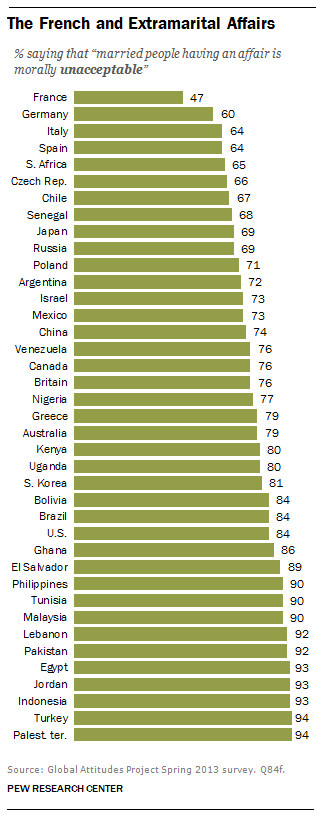
\includegraphics[width=0.95\linewidth]{images/Libro-img016.jpg}
  \begin{minipage}{\linewidth}
    \caption{Paesi dove l'infedeltà è più accettata}
  \end{minipage}
\end{wrapfigure}

Secondo i dati raccolti su base europea dall'IFOP (istituto francese di opinione pubblica) il 45\% degli italiani ha dichiarato di
aver tradito il partner almeno una volta contro il 43\% della Francia, il 39\% della Spagna e il 36\% della Gran
Bretagna. Di cui solo un 27\% di italiani si è pentito mentre in Francia e Germania 28\%, Spagna 36\% e Gran Bretagna 50\%. 

Secondo una ricerca mondiale condotta da Pew
Research\endnote{\raggedright\url{https://www.pewresearch.org/fact-tank/2014/01/14/french-more-accepting-of-infidelity-than-people-in-other-countries/}} il nostro paese appare molto più laico di quello che si pensa, infatti solo il 64\% degli italiani pensa che
l'infedeltà sia moralmente inaccettabile, piazzandosi al terzo posto dietro a Germania 60\% e
Francia 47\%, contro l'84\% degli USA e il 76\% dei Britannici. Sempre l'IFOP
ci riporta che, nonostante l'Italia sia la patria del cattolicesimo, per il 56\% degli italiani si
può essere innamorati del proprio partner e comunque tradirlo e, per il 63\% si può essere innamorati di due persone
contemporaneamente. Il 21\% degli intervistati ha una stabile e duratura relazione con l'amante,
mentre il 41\% ha avventure occasionali. Il 43\% degli infedeli si aspetta di essere perdonato e in effetti le
statistiche ci dicono che questo accade nel 70\% dei casi. Il 76\% degli Italiani dichiarato che rimanere fedeli è
possibile, tuttavia, i dati sull’infedeltà suggeriscono che questa norma morale non sempre corrisponde ai comportamenti. Come tradimento viene considerato: baciare alla francese (77\%), avere rapporti orali/sessuali (89\%), che raggiunge il 92\% se la pratica è regolare. 

\needspace{4cm}
\begin{figure}[H]
  \centering
  \begin{tikzpicture}
    \begin{axis}[
      ybar,
      xlabel={Categoria},
      ylabel={Valore},
      xtick=data,
      symbolic x coords={1, 2 - 3, 3 - 9, 9 - 25},
      ]
      \addplot coordinates {(1,27) (2 - 3,36) (3 - 9,58) (9 - 25,49)}; 
      \addplot coordinates {(1,21) (2 - 3,11) (3 - 9,46) (9 - 25,36)}; 
      \legend{Maschi, Femmine}
    \end{axis}
  \end{tikzpicture}
  \caption{Sondaggio IPSOS che mostra la percentuale di tradimento (y) nei vari anni di matrimonio (x) in Italia. Tra il secondo e il terzo anno di matrimonio, la disparità nei tassi di tradimento tra maschi e femmine tende ad aumentare, un periodo in cui generalmente nasce il primo figlio. Questa nuova fase può essere vissuta in modo differente dai due partner: in alcuni casi, l'impegno totale della donna nel nuovo ruolo di madre può portare a un cambiamento nelle attenzioni percepite dal partner, una dinamica talvolta espressa dai mariti come una 'trascuratezza'}
\end{figure}

Non è una questione di genere, infatti guardando diverse zone del mondo e periodi storici, possiamo trovare alcune
tribù, come quella in degli zo'é in Amazzonia che sono poligami sia gli uomini che le donne, anche se non possiamo generalizzare universalmente. Nella
società zo'é tutti sono eguali, e per tradizione non esistono leader.

Essere in una coppia aperta, di per sé, non rappresenta un problema morale: in un certo senso non si fa nulla contro il partner, ma semplicemente qualcosa con un’altra persona. Che si esca con un amico o si vada a letto con un amante, la quotidianità dell’altro non cambia automaticamente.

Il punto critico, però, non è l’azione in sé, ma l’accordo implicito che regola la relazione. Se non si è chiarito insieme che si è in una coppia aperta, l'altro, credendo nel patto di esclusività, rinuncerà a certe possibilità, convinto che anche noi lo stiamo facendo. In questo caso, il tradimento mina la libertà dell’altro senza che lo sappia.

Proviamo a fare lo sforzo di prendere in considerazione l'idea che la monogamia, o l'esclusività nei rapporti, possa persistere non solo per ragioni puramente razionali, ma anche perché profondamente radicata in dinamiche emotive come il desiderio di sicurezza, l'intimità esclusiva, la gestione della gelosia e la prevenzione della paura dell'abbandono o il bisogno di controllo.

Allo stesso tempo, quando proviamo attrazione per un’altra persona, sentiamo il bisogno di giustificarci o colpevolizzarci, come se il desiderio fosse una minaccia alla relazione. Ma l'idea che 'se desidero qualcun altro, allora c'è qualcosa che non va con il mio partner' è una convinzione che può essere profondamente influenzata dalla cultura monogama, piuttosto che essere una verità universale e intrinseca alla natura del desiderio.

D’altronde, siamo convinti che se fossimo con una persona idealizzata, come una celebrità, non proveremmo attrazione per altri. Ma la realtà dimostra il contrario: anche chi ha avuto relazioni con persone bellissime, famose o carismatiche ha sperimentato il desiderio per altri e, in alcuni casi, ha tradito. Questo suggerisce che il desiderio non si spegne con la mera idealizzazione, poiché è una forza complessa che non è sempre puramente razionale e può manifestarsi verso più individui.

\begin{mdframed}[linewidth=1pt]
A chi piacciono le donne magre e gli uomini muscolosi?

Secondo uno studio dell'Università di Saint Andrews, in Scozia sono in pochi ad apprezzare queste caratteristiche. Con
un campione di 146 uomini e donne eterosessuali di età compresa tra i 18 e 31 anni è stato chiesta ai partecipanti di
guardare delle immagini e scegliere quelle che preferivano come fisico ideale per se stessi e per il loro partner per
una relazione breve e quello per una relazione lunga. Gli uomini hanno sopravvalutato l'aspetto muscoloso nelle
preferenze delle donne, e le donne hanno sopravvalutato la magrezza nel corpo femminile. Inoltre, le percezioni errate
erano più marcate quando si pensava a relazioni più brevi.
\end{mdframed}

Secondo uno studio della Florida State University pubblicato nel 2018, in alcuni casi un aumento dell'autostima legato alla soddisfazione sessuale nella coppia può coincidere con una maggiore propensione al tradimento, ma questo fenomeno è influenzato anche da altri fattori psicologici e relazionali. Altre volte invece succede l'opposto. Siccome non ci si sente meritevoli di amore,
inconsciamente si cerca un'avventura, anche dando poca attenzione al non essere scoperti, proprio
per distruggere quella relazione e giustificare quello che si pensava. La profezia che si auto avvera.
Secondo una ricerca condotta da Selterman e il suo team nel 2023, è emerso che alcuni individui possono provare amore verso il proprio partner e, allo stesso tempo, intraprendere rapporti extraconiugali, senza necessariamente sperimentare sensi di colpa. Questo porta a una riflessione amara che contraddice l'idea comune secondo cui l'infedeltà è sintomo di problemi nella relazione. L'amore può non bastare a garantire la fedeltà e, in alcuni casi, il desiderio sessuale può prevalere sull'amore stesso\endnote{\raggedright\url{https://www.ncbi.nlm.nih.gov/pmc/articles/PMC10069361/}}.

Non possiamo quindi decidere di essere o non essere attratti da una persona, possiamo però, scegliere di non farlo
diventare un problema cosi da avere più energie cognitive da dedicare a come gestire la situazione.

Nel racconto biblico dell'adultera, quando le persone stanno per lapidarla, Gesù dice: Chi è senza peccato scagli la
prima pietra. Pian piano i presenti iniziarono a far cadere le pietre a terra e, i primi furono i più anziani e per
ultimi i giovani. Questo perché gli anziani, con più esperienza, riconoscono le contraddizioni
dell'essere umano e sanno, che anche loro, in una certa situazione, avrebbero potuto compiere
questo gesto sbagliato. L'atto del perdono, è un atto di riconoscimento verso se stessi e delle proprie contraddizioni.

Possiamo vedere le cose per ciò che sono, un infatuazione è
un infatuazione, non ha altri messaggi nascosti, inconsci, non significa ne che la nostra relazione stia andando male,
ne che lei/lui sia giusta/o per noi. Secondo Esther Perel in Così fan
tutti\endnote{\raggedright\url{https://www.amazon.it/dp/B07CT6NRQ5/}}, quando un matrimonio finisce per iniziare una nuova storia con
l'amante, questa nuova coppia tenderà ad avere una stabilità minore rispetto a quelle iniziate in altri modi. Sembra strano, in
quanto si è messo a rischio così tanto con un divorzio e tutto ciò che ne consegue. Ma quando subentra la quotidianità
del “porta fuori la spazzatura” e “abbassa la tavoletta” la magia è potrebbe svanire. Il problema non è quindi la
quotidianità che è inevitabile, ma etichettare la quotidianità alla banalità, alla noia, al problema a qualcosa di sbagliato che non dovrebbe esistere tra innamorati\endnote{\raggedright\url{https://www.stateofmind.it/2021/01/tradimento-relazioni-sentimentali/}}.

la Psicologia dell'adulterio è falsata dalla morale convenzionale che nei paesi monogami,
l'attrazione per una persona non possa coesistere con il serio affetto per
un'altra. Ma la realtà è più complessa di così - Bertrand Russell (Matrimonio e
morale\endnote{\raggedright\url{https://www.amazon.it/dp/B08ZNR576M}}).
Alcuni dati osservano quanto il fenomeno sia diffuso, superando anche il 40\% in alcuni paesi monogami\endnote{\raggedright\url{https://worldpopulationreview.com/country-rankings/infidelity-rates-by-country}}.
Sulla confessione del tradimento ci sono diverse teorie, alcuni sostengono che sia preferibile non confessare. I dati hanno permesso di avere diversi campioni di coppie con tradimenti confessati e non e, in alcuni casi, le coppie riescono a superare episodi di infedeltà e mantenere la relazione, ma l'esito varia molto a seconda delle circostanze e delle modalità con cui l'infedeltà viene gestita. Il rischio della confessione può non portare a qualcosa di positivo, ma solo al ferire l'altra persona. La confessione per qualcuno potrebbe essere solo un condividere e alleggerirsi un po' di questo dolore e senso di colpa. 
Ogni caso poi va visto separatamente, se il tuo partner potrebbe scoprirlo, o potrebbe sentirsi umiliato/a perché persone in comune potrebbero saperlo, è giusto che venga a saperlo da voi piuttosto che in modo ancora più spiacevole da altri.

Molte volte il disagio che sentiamo non è tanto per via dall'attrazione che sentiamo per
un'altra persona, ma il sentirsi sbagliati, diversi, da quello che culturalmente viene ritenuta la
norma, ovvero la monogamia in questo caso, ma il discorso può essere esteso a molti disagi. Oltre a
questo, bisogna comunque fare una scelta e, come spesso accade, ogni scelta comporta una rinuncia. Da una parte
chiudere la relazione principale con tutto ciò che ne comporta, divorzi, figli, casa ecc…
dall'altra parte rinunciare all'altra relazione con la perdita
dell'effetto vivificante e dell'arricchimento che potrebbe portare. 

Per concludere non so cosa sia meglio, forse dipende da persona a persona, ci sono pro e contro in entrambe le scelte,
quello che importa è che entrambi siano d'accordo e consapevoli della propria scelta. Qualsiasi
cosa decidiamo essere giusta per noi, non deve essere un modo per fuggirsi. Ad esempio per qualcuno il poliamore
potrebbe essere un modo per non impegnarsi, per altri, la monogamia è la scelta che non riceverà critiche dall'esterno.

\noindent \textbf{\large Può durare? E come?} \\
Secondo Massimo Recalcati un amore dura quando un corpo sa rivelarsi sempre nuovo, come un libro o una canzone che,
anche dopo anni, non via ha ancora stufato. Un'altra caratteristica, contraria
all'amore romantico della televisione che ci ha imposto un immaginario romantico irrealizzabile è
la solitudine. È importante ritagliarsi dei momenti di solitudine per rimanere due individui distinti, con le proprie
personalità, riuscendo a non fondersi in un unico piatto elemento. Una coppia esiste non per fondersi, o per avere
interessi comuni. Ma per realizzare la propria natura. Anzi, a volte avere interessi comuni potrebbe essere uno
svantaggio, perché si avrebbe meno tempo per stare da soli, cosa controintuitiva ma necessaria. Questo comporta che ci
saranno delle differenze tra i due partner e, alcune di queste potrebbero essere etichettate come difetti.
L'errore è aspettarsi il principe azzurro o l'equivalente femminile,
perfetto, senza difetti, perché questo ci potrebbe portarci a voler cambiare l'altro. Molto
spesso capita di allontanarsi dal partner perché “è cambiato” è anche possibile che il nostro partner fosse sempre stato così, solo che non
volevamo vederlo, perché ci siamo innamorati dell'innamoramento invece che della persona. Se
chiedessimo a una persona, cosa ti piace del tuo partner? E lei rispondesse: mi porta fuori a mangiare, mi compra i
fiori, mi dice cose carine ecc… Noteremmo che non ci ha detto molto di cosa le piace di lui, ma solo cosa lui fa per
lei. 
Vorresti che il tuo compagno/a ti dica le cose carine? Ma forse non è nella sua natura\endnote{\raggedright\url{https://www.youtube.com/watch?v=tRbGdjIgLE4}}.
Come abbiamo visto, quando cerchiamo di cambiare l'altro, potremmo ottenere
l'effetto paradossale di ottenere l'esatto contrario, ad esempio, una persona
fedele potrebbe diventare un traditore. In amore o ti fidi o non ti fidi, perché scovare un tradimento è più difficile di
quanto si pensi. Se cerchiamo prove che confermino un sospetto, troveremo cose neutre ma che dal nostro punto di vista
saranno invece sospette, portando anche un innocente ad apparire come un traditore. Una buona relazione non ti limita,
non ci sono giochi di potere, ricatti: se mi ami allora… O ad esempio, dare al partner tutto ciò che vorremmo che
ci desse in modo da pretendere che anche quest'ultimo ricambi e, facendolo sentire in colpa
qualora non soddisfasse le nostre tacite richieste. Ignorando che magari anche il nostro partner sta dando alla
relazione quello che lui vorrebbe ricevere, in quanto crede che possa far piacere, anche se non in linea con quanto
aspettato dall'altra parte, generando così un senso di inadeguatezza nonostante questo impegno mal
orientato, causa della cattiva o assente comunicazione.

Possiamo capire cos'è importante per noi e, se il nostro partner è in linea con questi desideri, dovremmo imparare ad apprezzare o, quantomeno accettare i suoi difetti. Di conseguenza il litigare non diventa un campanello d'allarme che segnala un problema
nella coppia, ma è la naturale dinamica di qualsiasi tipo di relazione che dura nel tempo. Anzi, al contrario se si
litiga poco potrebbe celarsi un'eccessiva accondiscendenza da parte di uno dei due partner. Il
problema è quando si litiga troppo e male, questo logora il rapporto.
L'ideale, più che litigare, è cercare di discutere, in maniera assertiva, cercando di dire quello che dobbiamo dire ma tenendo dei toni contenuti e senza essere offensivi.

Secondo uno studio della Northwestern University c'è un buon esercizio che permette di allenarci a vedere i motivi del
disaccordo e, dura solo sette minuti per tre volte all'anno. Bisogna scrivere del più recente
conflitto avuto con il partner assumendo il punto di vista di un'ipotetica terza persona che desidera il bene di
entrambi. Le coppie che hanno svolto questo esercizio non litigavano meno delle altre, ma tornavano più facilmente ad
uno stato di serenità.

Capita spesso di dire che incontriamo sempre le persone sbagliate. Se succede sempre però potremmo avere una responsabilità in questi episodi. 
Ad esempio: un individuo che si ritiene vulnerabile, per via delle sue esperienze passate nei
momenti di difficoltà, in un momento di stress, potrebbe porsi con rabbia, suscitando nel suo interlocutore un normale
distanziamento, freddezza, o abbandono, confermando così l'idea che aveva di sé stesso.\endnote{\raggedright\url{https://www.stateofmind.it/2020/06/attaccamento-disregolazione-emotiva/}}.

\begin{mdframed}[linewidth=1pt]
Qual è la durata ideale di un rapporto sessuale?

Secondo un sondaggio del 2008 pubblicato sul Journal of Sexual Medicine, terapeuti sessuali statunitensi e canadesi indicano una durata media “sufficiente” del rapporto penetrativo tra 7 e 13 minuti, ma si tratta di una media statistica e non di una misura ideale valida per tutti. La soddisfazione sessuale dipende da molte variabili soggettive, emotive e relazionali. In alcune persone, una durata troppo prolungata può talvolta generare distrazione o affaticamento, mentre sotto i 7 minuti è probabile che almeno uno dei due partner resti insoddisfatto.
Un altro studio, dell’Università di York in Canada, sostiene che il sesso programmato può essere tanto appassionato e gratificante quanto quello spontaneo. Nonostante la percezione comune che il sesso spontaneo sia più soddisfacente, i risultati di due studi suggeriscono che il sesso programmato può talvolta superare le aspettative di soddisfazione nella vita reale.
\end{mdframed}

Se ci sono dieci cose positive e una negativa, non facciamo diventare questo unico difetto il tutto di quella persona.

Quali sono i motivi più frequenti che possono portare alla rottura di una coppia?
\endnote{\raggedright\url{https://www.stateofmind.it/2021/07/relazioni-sentimentali-durature/}}

\begin{enumerate}
\item Soldi: un partner disapprova le spese dell'altro\newline
Possibile soluzione: si può discutere per stabilire un budget per le spese personali o extra
\item Sesso: ci si accusa di essere troppo pigri o inibiti \newline
Suggerimento: comunicazione
\item Gelosia\newline
Soluzione: Senza fiducia è difficile che una comunicazione possa funzionare
\item Tempo libero: dove andiamo, film, serie TV, a volte nascondono un modo per stabilire chi comanda \newline
Suggerimento: fare un po' per uno trovando il bello nelle scelte altrui
\item Parenti \newline
Suggerimento: cercare di frenare i genitori
\item Figli
\item Amici del partner \newline
Suggerimento: tolleranza
\item Casa e faccende domestiche \newline
Suggerimento: fare una tabella delle mansioni
\item Animali domestici
\end{enumerate}
Come spesso si legge, effettivamente, uno degli strumenti per riuscire a mantenere un buon rapporto è la comunicazione,
che non significa parlare tanto. Come scritto in L'arte di non amareggiarsi la
vita\endnote{\raggedright\url{https://www.amazon.it/dp/B00B0ZN91G} }, un giorno alla settimana compilare la "Lista
di suggerimenti con amore" e consegnarla al proprio compagno. Questa lista conterrà ciò che vorremmo cambiare del nostro partner. La peculiarità di questa lista è che ogni suggerimento va concluso con questa
frase: "…ma se non lo farai, ti amerò ugualmente per il resto dei miei giorni". 

La sessuologa Emily Nagoski
consiglia di ritagliarsi uno spazio, volontariamente, dove ci si mette a letto, sentendo il contatto della pelle del
partner, per creare l'atmosfera e far nascere il
desiderio\endnote{\raggedright\url{https://www.ted.com/talks/emily_nagoski_how_couples_can_sustain_a_strong_sexual_connection_for_a_lifetime}
}.
Emmanuele Jannini, sessuologo e docente all'Università dell'Aquila. «Noi studiosi diciamo che una coppia che non lo pratica è come se fosse muta e sorda, ma ciò non toglie che due partner possano stare bene insieme anche senza quel canale di comunicazione. È vero che molte coppie "scoppiano" perché non c'è più intesa sessuale, ma vuol dire che non sono riuscite a trovare altri modi per comunicare. Non mi stupisce che le ricerche in questo campo diano risultati contrastanti».

Se si ha meno voglia di fare sesso, non significa che le cose stiano andando male. Stando spesso assieme è normale che
il desiderio si affievolisca. Inoltre, come spiega Yuri Ohlrichs, capita di associare al sesso nelle relazioni a lungo
termine all'avere dei figli, e magari, in questo momento non ne senti il bisogno. Anche qua
percepiamo più il problema in relazione agli altri e a ciò che riteniamo dovrebbe esserci piuttosto che della questione
in sé. Non tutte le relazioni sono uguali e con i medesimi bisogni o che le vostre serate sul divano debbano per questo
sembrarvi meno preziose rispetto a coppie con una vita sessuale più
attiva\endnote{\raggedright\url{https://www.vice.com/it/article/xgdv4z/calo-desiderio-sessuale-in-coppia}}.

\begin{mdframed}[linewidth=1pt]
Possono essere utili le pause di riflessione e i tira e molla?

No secondo un team di studiosi delle università del Missouri e dell'Ilinois. Analizzando un campione di 545 persone
hanno notato più alti livelli di ansia e depressione che alla lunga portano al deterioramento del rapporto. I motivi che hanno portato all'allontanamento possono persistere anche dopo la fine del rapporto, soprattutto se non vengono elaborati consapevolmente. Non sempre una pausa porta a cambiamenti significativi, soprattutto se non è accompagnata da una riflessione autentica o da un confronto costruttivo.
\end{mdframed}

Ne il segreto dell'amore felice\endnote{\raggedright\url{https://www.amazon.it/dp/B00GH162G2/}} ho trovato dei
pensieri che si fondano sul non farsi domande riguardo i temi dell'amore, liberarsi dai giudizi e
vivere le esperienze per come sono. Non chiedersi se siamo innamorati, non dirlo agli altri per non rischiare di far sfumare quello
che proviamo. Se analizziamo e riempiamo di giudizi i nostri sentimenti, rischiamo di rovinarli. Non sforziamoci di
farlo durare se vogliamo che duri, questo potrebbe farci comportare in maniera esagerata, allontanado l'altra persona.
Non pretendere di innamorarti “come una volta”. Non esiste amore con la “a” maiuscola o minuscola. Abbiamo una lista
delle caratteristiche che deve avere l'amore per essere con la “a” maiuscola:
l'età, interessi, hobby, aspirazioni, status, se vuole figli ecc…. Ma così invece di un sogno,
rischia di diventare una gabbia, perché se, quando incontriamo qualcuno, controlliamo la nostra lista e, se manca qualcosa allora
dobbiamo soffrire o lasciare perdere questa persona impedendoci questa esperienza.

Alcune persone lamentano di non riuscire a trovare storie serie, attribuendo la causa alla mancanza di impegno altrui. Tuttavia, talvolta, queste stesse persone possono essere attratte da dinamiche relazionali meno impegnative. In questo scenario, a causa di giudizi culturali negativi verso tali scelte, può svilupparsi una narrazione che attribuisce le difficoltà a fattori esterni, anziché riconoscere i propri bisogni o schemi inconsci.

Le persone che incontriamo sono la scintilla. Quando senti di innamorarti di un'altra persona, la tua mente non ti sta chiedendo di
scegliere tra le due persone. Ti sta solo mostrando che c'è un lato di te che vuole emergere\endnote{\raggedright\url{https://youtu.be/lPRLiwrUrNA}}. 

Nel suo libro possiamo trovare alcune storie. Una paziente racconta che da due anni ha una relazione molto
importante con un uomo più grande, sposato e con due figli e questa cosa la fa soffrire. Se una relazione diventa
dolorosa in alcuni casi può dipendere dall'aver introdotto le nostre definizioni e i nostri progetti di vita. Possiamo solo goderci le cose
come capitano, altrimenti rischiamo di trasformale in un inferno di aspettative che raramente si avverano. Una tua
parte si è innamorata proprio di questa situazione, forse non vuole che si trasformi in un matrimonio, non possiamo
sapere i suoi piani, possiamo viverla per come è. Non esistono scelte sbagliate per la nostra crescita. Noi facciamo le
scelte che facciamo perché in quel momento, per la nostra maturità avevamo bisogno proprio di questo. 
Detto così forse può sembrare qualcosa di magico, ma in realtà è abbastanza spiegabile. Quando ci troviamo di fronte ad una scelta difficile, la difficoltà è data molto spesso dalla mancanza di informazioni, dal non aver riferimenti passati e così via. Per fare una scelta più consapevole dovremmo quindi provare una delle due strade ma a volte è difficile tornare indietro per diversi motivi. A volte abbiamo così poche informazioni che potremmo fare una scelta a caso che sarebbe uguale, ma a meno che non utilizziamo una monetina, non sarà davvero casuale la nostra scelta. La nostra sarà infine una scelta "intuitiva", o per meglio dire, dipendente da una serie di concomitanze, come ad esempio le pressioni sociali esterne, la nostra biologia, l'idea che abbiamo imparato sulle cose, l'avversione o propensione al rischio, le nostre insicurezze e l'elenco potrebbe andare avanti all'infinito. Quel che è certo è che noi, alla fine di tutto abbiamo scelto quella cosa, non sapremo tutte le concause che ci hanno portato a quella decisione, ma sta di fatto che l'abbiamo scelta e siamo stati noi a farlo. Nell'atto pratico possono esserci scelte sbagliate con il senno del poi, ma per quanto riguarda la nostra maturità, la nostra crescita, avevamo bisogno proprio di prendere quella decisione, anche solo per poterla escludere in un futuro, per vivere senza rimpianti, o per fare scelte più consapevoli. In quel momento dovevamo fare quella scelta, per sapere se quella strada, che credevamo la più probabile, era davvero giusta per noi. Questo ci potrebbe portarci anche a conoscerci un pochino meglio e se in un futuro faremo scelte diverse, dipenderà da quello che abbiamo etichettato come "errore", che se non avessimo fatto in passato avremmo forse commesso nel presente. Non decidiamo casualmente, per esserlo davvero, dovremmo lanciare una monetina e, probabilmente, l'attimo prima di scoprire il risultato sapremmo cosa vorremmo. Magari ci diciamo: un po' spererei in questo risultato… 

\begin{mdframed}[linewidth=1pt]
Secondo uno studio della Northwestern University (Usa) un esercizio per mantenere alta la soddisfazione della coppia è
scrivere su un foglio di carta circa il conflitto più recente con il partner assumendo il punto di vista di
un'ipotetica terza persona che desidera il bene di entrambi. Lo studio ha osservato che un esercizio di sette minuti, svolto tre volte all'anno, può essere un valido strumento per migliorare la gestione dei conflitti e favorire un più rapido ritorno alla serenità all'interno della coppia, contribuendo a diminuire l'impatto negativo degli scontri.\endnote{\raggedright\url{https://www.focus.it/comportamento/psicologia/come-non-litigare-con-partner-salvare-crisi-coppia} }.
\end{mdframed}

\noindent \textbf{\large Comunicazione} \\
Ne gli uomini vengono da Marte le donne da
Venere\endnote{\raggedright\url{https://www.amazon.it/dp/B00AA6F2OI}} leggiamo di alcune
differenze comportamentali tra uomini e donne, che però non si conoscono, tendiamo così ad avere aspettative sbagliate.
Pensiamo che se il nostro partner non si comporta come faremmo noi, c'è un problema. 

Secondo John Gray quando un uomo affronta stress o problemi, tende a ritirarsi emotivamente per riflettere e trovare soluzioni da solo. Durante questo periodo, l'uomo può sembrare distante o poco comunicativo, ma è un processo temporaneo che gli permette di ritrovare l'equilibrio. Le donne, invece, affrontano lo stress cercando connessione emotiva. Quando si sentono sopraffatte, esprimendo i loro sentimenti condividendo le preoccupazioni con persone di fiducia. Questo processo le aiuta a elaborare le emozioni e a sentirsi comprese e sostenute.
Di conseguenza, secondo questa visione, gli uomini comunicano principalmente per risolvere problemi e trasmettere informazioni, mentre le donne lo fanno per connettersi emotivamente e costruire relazioni.
Una donna potrebbe interpretare il ritiro emotivo dell'uomo come disinteresse, mentre l'uomo potrebbe non comprendere il bisogno della donna di parlare dei problemi. Riconoscere e rispettare questi diversi approcci può favorire una maggiore empatia e connessione tra i partner.

Va precisato che seppur il libro di Gray abbia avuto un impatto significativo nella cultura popolare, le sue affermazioni non nascono da uno studio scientifico. Le differenze tra uomini e donne esistono, ma sono spesso minime e influenzate da fattori sociali e culturali piuttosto che da distinzioni biologiche nette. Pertanto, è importante considerare ogni individuo nella sua unicità, evitando generalizzazioni basate sul genere.

Diversi studi hanno cercato di indagare questi fenomeni nelle coppie durante i conflitti o, più in generale, in situazioni di stress. Questi studi hanno trovato il cosiddetto pattern "demand/withdraw": una persona (spesso la donna) tende a cercare connessione e a voler discutere il problema (demand), mentre l’altra (spesso l’uomo) si ritira cercando soluzioni in autonomia (withdraw)\endnote{\raggedright\url{https://www.frontiersin.org/journals/psychology/articles/10.3389/fpsyg.2023.1217513/full}} \endnote{\raggedright\url{https://pubmed.ncbi.nlm.nih.gov/39049455/}} \endnote{\raggedright\url{https://www.frontiersin.org/journals/psychology/articles/10.3389/fpsyg.2021.794942/full}} \endnote{\raggedright\url{https://psycnet.apa.org/buy/1991-01045-001}}. Queste tendenze sono medie statistiche e non valgono per tutti gli individui: esistono uomini che cercano il dialogo e donne che preferiscono il ritiro, anche in funzione dello stile di attaccamento e della personalità.

Tornando al libro di Gray, generalizzando, dare un consiglio a una donna è segno d'interesse. Per una donna, se una cosa funziona, può
funzionare ancora meglio. Mentre gli uomini, orientati alla soluzione, non cambiano qualcosa che funziona. infatti gli
uomini possono reagire male ai tentativi di correggerli o di cambiarli. I consigli non richiesti possono essere percepiti da
un uomo come mancanza di fiducia e competenza nelle sue capacità. Come se fosse rotto e andasse aggiustato. Quando una
donna, invece, esterna i suoi sentimenti, l'uomo talvolta pensa che sia in cerca di soluzioni più che di
comprensione. Così la donna potrebbe sentire sminuiiti i suoi problemi, perché percepisce che secondo l'uomo
si possano risolvere con un paio di consigli che gli sono venuti in mente in quel momento, perché è in questo modo
che comunica disponibilità. Alcuni uomini possono interpretare frasi come “Non usciamo mai” come la richiesta di una soluzione al suo cruccio. 
Così risponde: “non è vero, siamo uscititi settimana scorsa”. Di conseguenza lei la percepisce come un tentativo di sminuire i suoi sentimenti e di
liquidarla con una risposta facile. Quando un uomo vede che il suo consiglio e la sua disponibilità non sono stati
apprezzati, troverà difficile continuare ad ascoltare la sua compagna, perché non si sente utile, cosa per lui
importante, ignorando che per una donna invece, già il parlare dei propri problemi equivale a sollecitare una soluzione.
Quando gli uomini diventano consapevoli di questo aspetto, si sentono sollevati nel sapere che non è una loro
responsabilità risolvere i problemi delle loro compagne. Gli uomini quando parlano tendono a scambiare informazioni,
mentre le donne emozioni. Quando un uomo si ritira nel suo mondo interiore e, la donna se ne accorge,
siccome lei difficilmente reagirebbe in questo modo, mostra il suo interesse domandando se va tutto bene. In questo modo però, senza volere, sta bloccando un momento di introspezione a cui l'uomo potrebbe rispondere con un “va tutto bene”. Gli uomini solitamente tendono a chiudersi nel silenzio piuttosto che esternare un disagio e spiegare di aver bisogno solo di un po' di tempo per restare da soli. Una donna però può percepire questo silenzio, talvolta erroneamente, come un “non voglio parlare con te”. Uomini e donne vivono queste fasi ciclicamente. A volte gli uomini tendono ad
allontanarsi, per poi riavvicinarsi, magari proprio nel momento in cui la donna cerca maggiore intimità. Allo stesso
modo anche le donne ciclicamente possono sentire un vuoto, dove cercano amore, attenzioni e sostegno, per poi tornare nuovamente piene di energia e con molto da offrire. 

Quando uno dei due partner è troppo presente, per l'altro potrebbe diventare più faticosa la relazione, uscire assieme, le telefonate, impegni e così via. Così, senza accorgersi, si potrebbe creare una distanza. Altre volte succede, più per
l'uomo e la sua necessità di risolvere i problemi, che affiancandosi ad una persona poco indipendente, che negli anni non ha coltivato una solida rete relazionale e di interessi, senta la responsabilità di dover provvedere all'altra persona. Al contrario, persone troppo autonome
potrebbero lanciare il messaggio: io non ho bisogno di te. In questi casi il partner che percepisce questa distanza, che potrebbe aver contribuito a creare, anche se inconsapevolmente, potrebbe aggravare la situazione accusando il partner portandolo in alcuni casi a sentirsi come il problema, quando magari invece è stata una reazione
comprensibile. Quando la discussione inizia a far leva sui sensi di colpa, non porta necessariamente la ragione all'accusatore, ma quando si è coinvolti direttamente è difficile osservare queste dinamiche con lucidità e distacco, portandoci talvolta anche a credere di essere davvero noi il problema.

In una discussione per comunicare in maniera efficace possiamo seguire questi punti:
1. Validare le emozioni:
"Mi rendo conto che ti sei sentito ignorato ieri sera, e mi dispiace."

2. Esplorare con domande aperte:
"Cosa ti ha fatto sentire così? È stato qualcosa che ho detto o fatto?"

3. Esprimere il proprio punto di vista con rispetto:
"Ero davvero esausto e non me ne sono reso conto, ma non volevo ferirti."

4. Cercare soluzioni comuni:
"C'è un modo per trovare un compromesso che vada bene a entrambi?"

Ma perché uomini e donne sono così diversi? Lo psicologo John Gottman, uno dei più grandi studiosi della relazione di
coppia, ha tentato di dare una spiegazione in Intelligenza emotiva per la
coppia\endnote{\raggedright\url{https://www.amazon.it/dp/B00G6KL9DU}}. È stato osservato che lo stress può influenzare la produzione di latte nelle donne in fase di allattamento, suggerendo un possibile vantaggio evolutivo per chi riusciva a regolare più efficacemente le emozioni. Tuttavia, le differenze nei meccanismi di risposta allo stress tra uomini e donne sono complesse e influenzate anche da fattori culturali, oltre che biologici. 
Secondo le osservazioni di John Gottman, durante i conflitti alcuni uomini possono mostrare una maggiore attivazione fisiologica, che rende difficile calmarsi e comunicare. Le donne, in media, tendono più spesso a cercare strategie di regolazione emotiva orientate alla riconciliazione, ma si tratta di tendenze generali che non valgono per tutti i casi.
Per questo motivo gli uomini tendono ad andare di più sulla difensiva durante un conflitto, talvolta in maniera vittimistica,
bellicosa o silenziosa.

Un altro tema frequente è quello che vede il nostro partner coinvolto in una disputa: se non condividiamo il suo punto
di vista dobbiamo dirglielo o dobbiamo sostenerlo? Entrambe le cose secondo John Gottman, ma con i giusti momenti.
Inizialmente il nostro partner si rivolgerà a noi per cercare aiuto emotivo e non necessariamente per un consiglio, quindi potremmo sostenerlo. Quando la carica emotiva sarà passata, allora potremmo, in punta di piedi, provare a fargli vedere il
nostro punto di vista. La base per affrontare i problemi è la stessa: Comunicare accettazione della personalità ma non del comportamento con il fine di trovare un compromesso.
Le persone sono spesso più propense a cambiare quando si sentono accettate e apprezzate per come sono. Se un vostro amico dimentica l'ombrello
in giro, semplicemente gli dite: “Hai dimenticato l'ombrello”, non ci salterebbe in mente di
dire: Ma che cos'hai? Non fai altro che dimenticare in giro gli oggetti. Per
l'amor del cielo, cerca di stare più attento! 

Esempio: due partner fermi sul problema dell'ordine della casa. Lei vorrebbe che lui sia più ordinato,
mentre lui vuole dedicarsi alle sue cose nel tempo libero quando è a casa. Quali sono i desideri che stanno dietro
questa richiesta? Per lei un senso di ordine e, per lui, il bisogno di libertà a casa sua. Per trovare un compromesso
possiamo individuare le aree non negoziabili. Lei non può accettare i piatti e il bagno sporco, lui invece non vuole
rimettere in ordine le sue carte finito di lavorare, perché lo costringerebbe a riorganizzarle nuovamente il giorno
seguente. Fortunatamente le aree non negoziabili non sono in contrasto tra loro, così possiamo lavorare su delle aree
di flessibilità: Lei può vivere con un po' di disordine, a patto che il bagno e la cucina siano
puliti. Lui può lavare i piatti e il bagno a patto di non doverlo fare in continuazione. Lei non lo assillerà con la
mania dell'ordine più di una volta alla settimana, ma se lui non si comporterà come è stato
stabilito, lei raccoglierà tutto e glielo metterà sul pavimento del suo studio di casa. Lei probabilmente odierà sempre il disordine
e, lui odierà sempre l'ordine, per questo entrambi dovranno stare attenti di continuo a rispettare
i patti. Stare assieme richiede un certo impegno, contrariamente a quello che la filmografia ci ha insegnato. Sempre secondo John Gottman le coppie che funzionano condividono 5 ore o più di qualità alla settimana con il proprio partner,
inoltre, non bisogna avere paura della discordia o di litigare, questo infatti non è sinonimo che il rapporto stia
andando in una direzione sbagliata. Non sempre il diverbio si risolve discutendo all'infinito.
Molti rapporti durano felicemente nascondendosi delle cose che fanno arrabbiare l'altro. 
Tuttavia, ignorare sistematicamente i problemi può, a lungo andare, minare l’intimità e la comunicazione.
Altri ancora, quando litigano, chiudono la discussione, magari momentaneamente, o anche no e, ognuno si allontana per
dedicarsi ai propri hobby. Per qualcuno invece l'amore non è al primo posto spiega Ombretta
Cecchini\endnote{\raggedright\url{https://www.spreaker.com/user/dott.ssa\_ombrettacecchini/non-sei-la-sua-priorita} }. Una persona
potrebbe amare il volontariato e essere meno dedito verso il partner. Questo non significa essere egoisti, anaffettivi
o narcisisti. Non tutti sono uguali o hanno lo stesso modo di amare. Altri urlano e gridano, poi ad un certo punto uno
dei due tira fuori la lingua e fa il bambino per sciogliere la tensione, questo è quello che si chiama: tentativo di
riparazione. Spesso è controproducente affrontare un diverbio quando l'altro non ne ha alcuna
intenzione, magari è meglio aspettare un momento migliore, specie se l'altro sta facendo qualcosa
che gli piace. Insomma, la regola è che tante volte non c'è una regola, ogni coppia deve trovare
il suo modo, il suo equilibrio. Può essere utile però distinguere nella coppia i problemi risolvibili e quelli irrisolvibili che si presentano perpetuamente. Se l'altra persona non le piace una cosa e non c'è verso che le piacerà mai, è inutile insistere, quella persona ha tutto il diritto di avere le sue preferenze e l'unica cosa che possiamo fare è accettarlo o trovare un compromesso\endnote{\raggedright\url{https://youtu.be/dB3UNx96_RU}}. 

In Quiet\endnote{\raggedright\url{https://www.amazon.it/dp/8845294064} } di Susan Cain viene riportato un esempio dove un marito,
rassettato la cucina, la mattina seguente sente urlare: "Questa cucina è un porcile!" Entrando e
guardandosi attorno, si possono notare al massimo tre o quattro bicchieri in giro. La foga di quei momenti per Jennifer
è del tutto naturale, è il suo modo di dire: Cavoli, mi piacerebbe che tenessi un po' più in ordine la cucina. Se me lo
comunicasse in questi termini le risponderei: Piacerebbe anche a me, amore, scusami se non l'ho fatto. Invece in questo
modo aggressivo potrebbe sorgere una risposta altrettanto violenta. Nel nostro esempio però, il marito ha
riconosciuto che questo è il modo in cui la moglie si esprime e che non è poi la fine del mondo.

Gary Chapman ne i cinque linguaggi dell'amore\endnote{\raggedright\url{https://www.amazon.it/dp/8801023723} } ha individuato cinque
modalità che le persone ricercano nel proprio partner.

\begin{enumerate}
\item Parole di rassicurazione e apprezzamento: Se una moglie vuole che il marito imbianchi le pareti non deve porsi
pretendendolo in continuazione. Se lo si dice una volta, la persona ha l'informazione, dirlo altre mille volte spesso porta con sè il messaggio di una pretesa e imposizione autoritaria. Molto più efficace è invece comunicare apprezzamento per tutte le altre
cose buone che fa, come portare fuori la spazzatura.
\item Momenti speciali: Quando un coniuge critica il partner perché lavora troppo, o perché esce spesso con gli amici,
non sta dicendo che odia il suo lavoro, ma semplicemente vede in questo l'oggetto che sottrae a
lei o a lui il tempo che vorrebbe che venisse dedicato. Per queste persone, che ricercano momenti speciali da passare
assieme, anche parlare risulta difficile mentre si guarda la televisione, perchè cercano di dedicare ai giusti momenti una condivisione sincera.
\item Ricevere Doni: Non devono essere per forza dei doni costosi, anche in questo caso è il pensiero quello che conta.
\item Gesti di servizio: Fare qualcosa per l'altro come pulire, lavare, tagliare l'erba eccetera.
\item Bisogni fisici: Come ricercare carezze, abbracci o sesso ad esempio. 
\end{enumerate}
Come possiamo capire con quale linguaggio vorremmo che il nostro partner utilizzasse con noi? E quale vorrebbe che noi
utilizzassimo con lui o lei?

\begin{itemize}
\item Fare una lista delle cose che vorremmo dal partner: Quello che troviamo scritto non deve essere svolto per forza,
ma va preso in considerazione in quanto per l'altra persona rappresenta un modo di sentirsi amata.
\item Cosa ci ferisce? Gary Chapman suggerisce di portare attenzione a ciò che ci ferisce, a volte può essere più
rappresentativo rispetto a ciò che desideriamo. Quindi se ci ferisce quando il nostro partner ci scredita, forse il
nostro linguaggio d'amore è il primo. Se ci avvilisce ricevere pochi doni, forse il nostro linguaggio d'amore è il
terzo e, così via.
\item Come comunichiamo? Chiedersi quale linguaggio utilizziamo più frequentemente per esprimere amore al nostro
partner. Ricordiamo però che può capitare che una persona esprimi amore in un modo ma poi lo ricerchi in un altro.
\item Il partner ideale: Se pensiamo al nostro partner ideale o alla nostra relazione duranti i primi mesi, cosa ci
veniva dato che apprezzavamo di più?
\end{itemize}

Ma come dobbiamo comportarci se noi ci impegniamo verso il nostro partner ma lui o lei non fa altrettanto con noi?
Non dovremmo forzare il cambiamento negli altri, al massimo possiamo influenzare le dinamiche relazionali attraverso il nostro comportamento e modo di comunicare.
Si dovrebbe comunicare amore perché
si sente il bisogno di farlo, non perché così l'altro si sentirà in dovere di fare altrettanto.
Indicativamente comunque, quando ci si pone in maniera amorevole, dall'altra parte ci sarà una certa propensione a
ridarlo indietro, ma magari comunicato in un modo che non in linea con quello che cerchiamo. In questo caso, se vogliamo
che il nostro partner comunichi con noi, nel nostro linguaggio, dovremmo fare delle richieste specifiche, quindi evitare
di dire: vorrei passare più tempo assieme, ma preferire un meno generico: sabato vorrei fare una passeggiata con te in
questo posto di pomeriggio.

Giorgio Nardone in Correggimi se sbaglio\endnote{\raggedright\url{https://www.amazon.it/dp/8862209797} } punta
l'attenzione sulle cose che non si dovrebbero dire ma in cui troppo spesso inciampiamo, come ad
esempio: recriminare, rinfacciare o dire “te l'avevo detto”. Anche quando dici “ho rinunciato a questo per te”, hai potenzialmente preparato una rivalsa, un rinfacciare qualcosa, ponendoti in modo da avere potere sull'altro. Altre volte invece ci sono delle zone grigie, come il puntualizzare. Puntualizzare è giusto, ma se viene
fatto con troppa insistenza il nostro interlocutore non si sentirà più in un rapporto paritetico perché potrebbe
iniziare a supporre che gli stiamo insegnando come stare al mondo o, come dovrebbero andare le cose. A volte, queste
modalità sono più sottili da individuare come dannose. Frasi come: lo faccio solo per te, ci mettono in una condizione
emotiva ambivalente: Da una parte ci sentiamo di ringraziare il nostro interlocutore per la sua generosità, ma allo
stesso tempo ci sentiamo in difficoltà a farlo, in quanto questa gentilezza non è stata né desiderata né
richiesta, inoltre lo percepiamo come un sacrificio unidirezionale. Non dovremmo far pesare
all'altro quello che facciamo per lui. Non dire: lascia, faccio io o si, ok va bene, ma si poteva
fare di meglio, possono far sentire squalificate le capacità altrui.

Possiamo chiederci: Voglio trovare una soluzione/compromesso o voglio solo vincere il dibattito? 

\subsubsection{Perdono}
L'etimologia della parola perdono è formata dalle parole per e dono. Un dono che doniamo a noi
stessi e all'altro. Il perdono può aiutarci a liberarci dal rancore e dalla voglia di vendetta, facilitando il nostro benessere emotivo. 
Percepiamo il perdono come qualcosa che porta con sé un costo, una perdita, elevata a volte. Ma nell'ottica del
dono possiamo cercare di viverlo con gratitudine, anche se è più facile dirlo che farlo. Se perdoni accetti quello
che è successo e che le cose potrebbero non tornare più come prima. Al contrario infatti, se perdoni per manipolare l'altro, al
fine che tutto torni come prima, neghi questa genuinità di abbandono, rischiando di non perdonare per davvero.

Il perdono non vuol dire dimenticare. Non è un amnesia. Il concetto di perdono è espresso bene nella parabola del figlio
prodigo\endnote{Vangelo secondo Luca 15,11-32}. La parabola si riferisce al figlio di un uomo che scappa di casa
disobbedendo e sperperando tutti i soldi del padre. Ridotto alla fame il figlio torna a casa vergognandosi di quello
che ha fatto. Il padre lo accoglierà abbracciandolo e facendo una festa. Importante è lasciare il tempo
all'altro di accettare le scuse.

“Perdona gli altri, non perché essi meritano il perdono, ma perché tu meriti la pace” - Buddha

Se non ti senti di perdonare, non devi farlo per forza. Forse una parte di te vuole mantenere le distanze. Non
sentirti a disagio se non riesci a perdonare. Perdona solo se ti fa stare bene. Indicativamente comunque, secondo gli studi di Lee ed Enright, perdonare influisce
positivamente sulla nostra salute fisica\endnote{\raggedright\url{https://www.stateofmind.it/2021/06/perdono-salute-fisica/}}.

Non fare mai del bene se non sei preparato all'ingratitudine – Enzo Ferrari

Un idea ancora più dirompente l'ho sentita in una domanda posta a Sadhguru\endnote{\raggedright\url{https://www.youtube.com/watch?v=3UmEDNLyQYU}} dove una ragazza chiede: Perdonare le persone è difficile, come possiamo fare?
Per perdonare qualcuno devi prima criminalizzarlo e poi perdonarlo. 
Una persona ha fatto quello che ha fatto perché è il meglio che ha saputo fare, se avesse saputo fare di meglio in quel momento, lo avrebbe fatto. Quindi io ti accetto così per come sei, non c'è da perdonare. Se ti perdono, talvolta, è perché prima ti ho dato una colpa da cui poterti eventualmente assolvere. Nessuno è perfetto, puoi decidere di accettare e interagire con loro oppure no. Non giocare a fare d
Dio e dire chi ha la colpa e chi è perdonato. Se criminalizzi qualcuno, per quanto ti sforzi di perdonarlo rischi di continuare a percepirlo colpevole nella tua mente in una certa misura.
Se troviamo una persona egoista è perché forse ha avuto questi esempi e in un certo momento della sua vita questa sua strategia relazionale ha funzionato e, inconsapevolmente la ripropone non per farti volutamente del male, ma perché forse è solo quello che sa fare e tutti abbiamo comportamenti che possono non piacere agli altri.

\needspace{4cm}
\begin{mdframed}[linewidth=1pt]
Esperimento di Harlow sull'attaccamento tra madre e figlio 

\needspace{4cm}
\begin{wrapfigure}{i}{9cm}
  \centering
  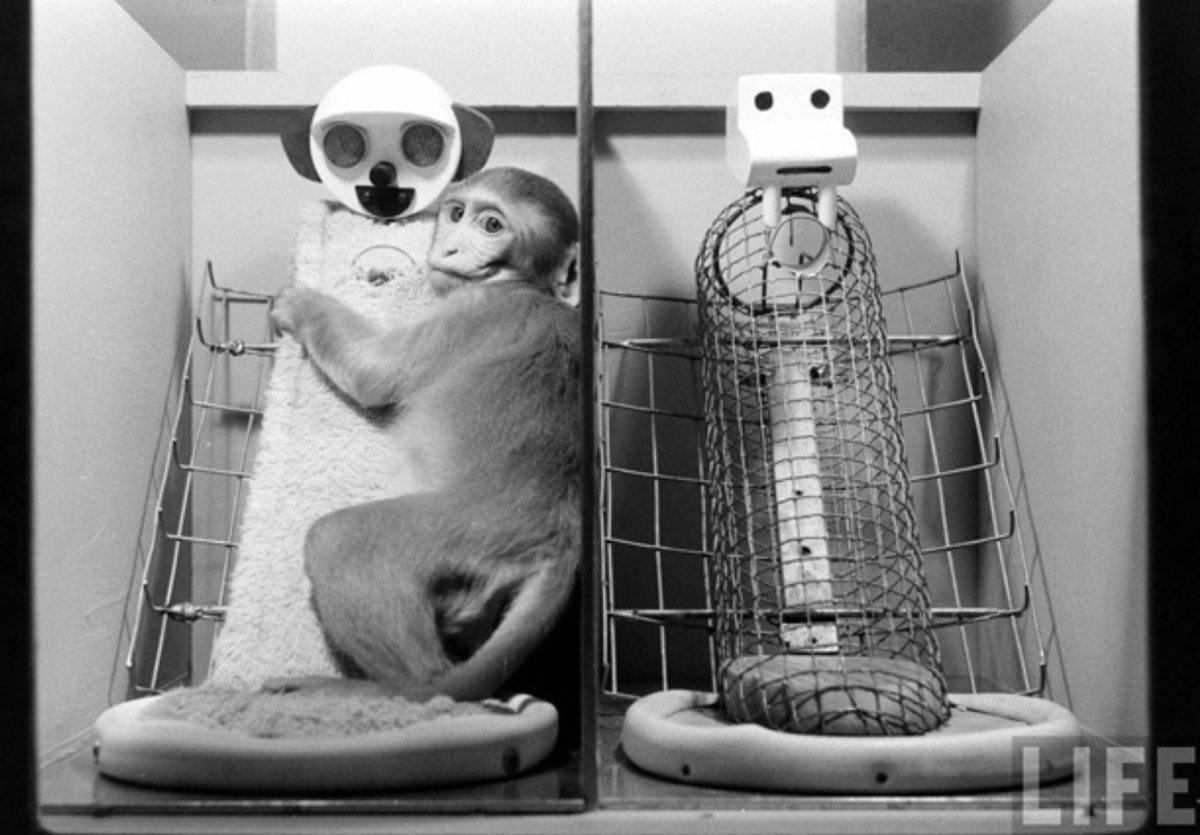
\includegraphics[width=0.95\linewidth]{images/Libro-img017.jpg}
  \begin{minipage}{\linewidth}
    \caption{Esperimento di Harry Frederick Harlow}
  \end{minipage}
\end{wrapfigure}

All'epoca dell'esperimento, nel 1958 si pensava che il legame tra madre e
figlio dipendesse in misura maggiore per il neonato da un soddisfacimento dei propri desideri primari, come
mangiare e bere. Harry Frederick Harlow per il suo esperimento prenderà dei neonati di macachi invece di umani, siccome
sono autonomi nel movimenti già tra i 2 e i 10 giorni di vita e dimostrano affettività in modo simile a noi. Harlow
costruisce poi due madri surrogate dove la base è un cilindro fatto da una rete metallica e una testa di legno. Una
ricoperta da un panno caldo e morbido l'altra dotata di un meccanismo per nutrire il piccolo.
L'esperimento, è stato riproposto diverse volte e in alcuni casi dotavano la “madre morbida” anche
del dispositivo di nutrimento. In qualunque caso i piccoli di macaco hanno scelto la “mamma morbida” spostandosi
verso l'altra solo quando avevano fame.

Questa è per Harlow una scoperta sensazionale, ne deduce che non c'entrava il soddisfacimento della fame e della sete. La vera funzione dell'allattamento, è quella di avere un contatto intimo
con la madre. Anche in momenti di paura, indotta con un giocattolo meccanico i piccoli macachi si rifugiavano dalla “mamma morbida”. Nei momenti di tranquillità i macachi si sentivano liberi di scoprire
l'ambiente circostante solo in presenza della madre surrogata. Quando la madre viene tolta
dall'ambiente del macaco, quest'ultimo si mostra impaurito restando
accovacciati e iniziando a dondolare. Harlow mette così in crisi le teorie dell'epoca
sull'attaccamento ma anche a livello socioeconomico, minando la certezza assoluta che le madri
debbano restare a casa dal lavoro dopo il parto, in quanto, anche l'uomo può soddisfare i bisogni affettivi del neonato.

Purtroppo anche questo è stato un esperimento un po' crudele, di cui abbiamo alcune testimonianze
video\endnote{\raggedright\url{https://www.youtube.com/watch?v=\_O60TYAIgC4} }
\endnote{\raggedright\url{https://www.stateofmind.it/2016/04/attaccamento-esperimento-di-harlow/}}.
\end{mdframed} 

\noindent \textbf{\large Quando è finita?} \\
Ma come si fa a capire quando una relazione è finita? A volte ci siamo talmente dentro da non riuscire a vedere la nostra relazione in maniera abbastanza 
obiettiva. La paura di restare soli, la routine,
l'abitudine, ci portano a vedere questo come la nostra normalità, finendo talvolta per accettare situazioni asfissianti e tossiche. 

Di seguito alcuni segnali\endnote{\raggedright\url{https://www.ted.com/talks/katie_hood_the_difference_between_healthy_and_unhealthy_love}}:

\begin{itemize}
\item La relazione non ci sta potenziando ma ci sottrae energie.
\item I litigi sono più frequenti e immotivati 
\item Il partner vi sottrae da amicizie, passioni, famiglia, facendo commenti sulle persone e, facendo insorgere il germe del dubbio anche se infondato.
\end{itemize}

\begin{mdframed}[linewidth=1pt]
Marcel Proust scrivendo La prigioniera mostra il protagonista rinchiudere Albertine, di cui era innamorato, per gelosia e, vedere l'attrazione per
lei scesendere. In questo paradosso dell'amore siamo gratificati e attratti dal partner che sceglie noi, nella misura in cui lui o lei è libera ma, in quanto libera, può decidere di non sceglierci più.

La gelosia inoltre, per qualcuno è conferma dell'amore verso di noi, ma se troppa e protratta nel
tempo, potrebbe portarci a desiderare proprio ciò che il partner vuole prevenire. Essere costantemente oggetto di sospetto e accuse di infedeltà può generare frustrazione e distanza emotiva e, in alcuni casi può contribuire a comportamenti disfunzionali, anche se non rappresenta una causa diretta e universale dell’infedeltà.

In un caso riportato in Amore e disamore\endnote{\raggedright\url{https://www.amazon.it/dp/8833316432} }, a fine terapia di coppia dove
lei ha tradito lui, quest'ultimo, ritrovata la serenità, si trova a dire alla sua compagna,
facendole l'occhiolino, come gesto d'intesa: “esci pure e, divertiti”. Il
terapeuta gli fa notare che, senza saperlo, questo gesto è stato molto strategico, perché così dicendole ha realizzato
un paradosso comunicativo: 'Se sono io a spingerti fra le braccia di un altro, non solo ti tolgo
la componente trasgressiva, ma mi dimostro molto sicuro di me stesso'.
\end{mdframed}

Ma quando finisce una relazione, riusciamo a migliorare per la prossima? E a non riproporre più gli stessi comportamenti? Spesso, senza un lavoro consapevole, si osserva una tendenza a replicare i modelli relazionali appresi, poiché sono profondamente radicati nel nostro modo di interagire\endnote{Johnson, M. D., \& Neyer, F. J. (2019). (Eventual) stability and change
across partnerships. Journal of Family Psychology, 33(6), 711–721. doi:10.1037/fam0000523
\raggedright\url{https://pubmed.ncbi.nlm.nih.gov/30802084/}}
\endnote{\raggedright\url{https://www.stateofmind.it/2019/09/relazioni-sentimentali-cambiamento/}}. Possiamo cercare di cambiare diventando consapevoli di noi stessi e dei nostri difetti, in modo da prestare più facilmente attenzione,
quando questi nostri comportamenti si manifestano e, a quel punto trovare modi per intervenire. 

Quando una relazione finisce siamo attratti dal fuggire il dolore, che ha invece motivo d'esserci,
solitamente in modi dannosi, dal chiodo scaccia chiodo all'odiare tutto ciò che è stato. Se
impariamo a stare nel dolore, senza giudizio, possiamo portare a casa qualcosa per il futuro.

La crisi spesso non è crisi di coppia, ma crisi di uno degli elementi della coppia. Per curare
una crisi di coppia bisogna partire da curare noi stessi. Dedichiamoci più tempo evitando di pensare che tutto tornerà come prima. Forse non succederà e, la nostra relazione andrà in altri territori in altre direzioni inesplorate.

\begin{mdframed}[linewidth=1pt]
I maschi pensano solo a quello!

Uno dei fattori che può influenzare dipende da un
fattore religioso e culturale che associa la vergogna al sesso. Con il tempo sta diventando meno un tabù, per entrambi i sessi, ma c'è ancora un divario che pone la donna in una misura di maggiore vergogna rispetto all'uomo. Il secondo motivo è evolutivo. Biologicamente
non siamo troppo diversi dagli uomini delle caverne che dovevano lottare per la propria sopravvivenza. Al fine di
conservare la specie, la riproduzione è necessaria, ma per la femmina il compito è più gravoso e rischioso. Infatti una gravidanza richiede più energie, risorse, si può morire di parto, anche quando nasce il
bambino, c'è l'allattamento, le cure, ecc… Dal punto di vista evolutivo, i maschi della specie umana possono aver sviluppato una maggiore propensione alla ricerca di opportunità sessuali, in parte perché il loro investimento biologico immediato nella riproduzione è inferiore rispetto a quello femminile\endnote{Trivers, R.L. (1972). Parental investment and sexual selection. In B. Campbell (Ed.), Sexual selection and the descent of man (pp. 136–179). Chicago, IL: Aldine}
\endnote{\raggedright\url{https://www.stateofmind.it/2020/03/attrazione-sessuale-riconoscimento/}}.

Anche per questi motivi, alcuni studi mostrano come il desiderio sessuale all'interno della coppia tende a diminuire
maggiormente per le femmine rispetto ai maschi, soprattutto dopo la gravidanza e il parto. Questo può portare al
declino della soddisfazione relazionale della coppia\endnote{McNulty, J. K., Maxwell, J. A., Meltzer, A. L., \&
Baumeister, R. F. (2019). Sex-Differentiated Changes in Sexual Desire Predict Marital Dissatisfaction. Archives of
sexual behavior, 48(8), 2473-2489. \raggedright\url{https://pubmed.ncbi.nlm.nih.gov/31471791/} }
\endnote{\raggedright\url{https://www.stateofmind.it/2020/04/cambiamento-desiderio-sessuale/} }.
\end{mdframed}

\noindent \textbf{\large Figli} \\
Non ne so molto di figli, ma ho comunque raccolto qualcosa, nel caso un giorno mi servisse.

\textbf{Rimpianti}

La letteratura scientifica riporta che il rimpianto legato alla genitorialità è un fenomeno minoritario ma significativo. In una ricerca condotta su campioni nazionali in Polonia, Germania e Stati Uniti si stima che tra il 8\% e il 17\% dei genitori esprimano rimpianto per aver avuto figli, con valori più elevati in Polonia, e tale sentimento risulterebbe associato a una maggiore incidenza di esperienze infantili avverse, peggioramento della salute mentale e fisica, burnout genitoriale e problematiche economiche o coniugali\endnote{\raggedright\url{https://pubmed.ncbi.nlm.nih.gov/34288933}}.

Parallelamente, uno studio pubblicato su Journal of Child and Family Studies ha analizzato strumenti per misurare il rimpianto genitoriale, confermando che vi è una correlazione tra questo stato d’animo e il burnout, la depressione e una minore soddisfazione di vita\endnote{\raggedright\url{https://link.springer.com/article/10.1007/s10826-024-02988-8}}. La ricerca però è limitata da un numero ristretto e non rappresentativo di partecipanti, con prevalenza di madri, e da un contesto socio-culturale molto specifico, che ne riduce l’applicabilità a popolazioni più ampie.

In conclusione, sebbene la maggioranza dei genitori non provi rimpianto, una fetta rilevante — fino al 1 su 6 — sì, e in questi casi le conseguenze psicologiche e sociali possono essere rilevanti.  

\textbf{Frasi diseducative}\endnote{\raggedright\url{https://www.vice.com/it/article/k7akpm/frasi-genitori-diseducative}}

\begin{itemize}
\item Abbandono

\begin{itemize}
\item Frasi

\begin{itemize}
\item “Se non ti sbrighi ti lascio qui”
\item “Se fai così la mamma/il papà va via”
\end{itemize}
\item Problema: Questo può far emergere l’ansia da separazione, che nei bambini piccoli può essere vissuta come una minaccia intensa e destabilizzante.
\item La soluzione: Il nostro obiettivo non è far sentire abbandonato nostro figlio ma che si velocizzi e non si
disperdi. Giriamo la frase al positivo, invece di “se non fai…” diventa invece “se fai questo…”, o ancora dire “ok, ti
do dieci minuti per finire con l'altalena e poi andiamo”, aiutano a imparare concetti importanti
come il compromesso.”
\end{itemize}
\item Minacce e ricatti

\begin{itemize}
\item Frasi

\begin{itemize}
\item "Guarda che se urli ti porto dallo psicologo/in collegio"
\item “Se non ti comporti bene vedi cosa ti faccio”
\item “Se non fai i compiti, non ti compro quel giocattolo”
\end{itemize}
\item Problema: Premi e punizioni, se mal utilizzati o eccessivi, possono essere poco funzionali. Il bambino, in certi casi, potrebbe focalizzarsi più sul premio/punizione che sul comportamento in sé, tendendo a soddisfare le aspettative dell'adulto senza comprenderne appieno la logica sottostante. Tuttavia, se impiegati con attenzione e in modo educativo, possono guidare il comportamento. Se un bambino commette un errore, può tornare a giocare solo dopo aver sistemato la situazione.
\item La soluzione: Sottolineare i comportamenti positivi, in modo che il bambino si soffermi a riflettere su questa
acquisizione positiva”. Allo stesso modo fare per i comportamenti negativi, spronando il bambino a migliorarsi. 
Le punizioni, se percepite come ingiuste o umilianti, possono aumentare comportamenti oppositivi e ridurre la motivazione intrinseca del bambino.
Invece di dire: “non puoi giocare al Pc perché non hai finito i compiti”, anticipare dicendo: 
“non appena avrai finito i compiti, potrai giocare”. O ancora dire: "bravi, che siete così tranquilli!" invece di "quanto durerà questa calma?".
O si potrebbe porlo sottoforma di gioco, dando 5 monete virtuali o giocattolo e dire: ogni volta che ti comporti male perdi un soldo e, a fine giornata ricevi un premio, come il gelato o una conseguenza.
\end{itemize}
\item Insegnamenti sulla morale

\begin{itemize}
\item Frasi:

\begin{itemize}
\item “È un mondo difficile, è meglio se lo impari subito”
\item "Mangia tutto che nel mondo ci sono bambini che muoiono di fame"
\item “Quando sarai grande potrai fare quello che vuoi, adesso no”
\end{itemize}
\item Problema: Secondo alcuni esperti, le frasi sulla morale possono essere più una esternazione delle difficoltà che prova
l'adulto, ma traslate sul bambino spesso in negativo e/o in maniera punitiva.
\item Soluzione: Per insegnare la morale può essere una buona idea raccontare o leggere delle storie.
\end{itemize}
\item Confronti con coetanei e adulti

\begin{itemize}
\item Frasi:

\begin{itemize}
\item “Perché non sei come tuo cugino, che è così ubbidiente?"
\item “Sei come tuo padre/tua madre”
\item “Faccio io, che tu non sei capace”
\end{itemize}
\item Problema: rischiamo di intaccarne l'autostima e la sicurezza del bambino, necessarie per
affrontare il futuro. 
\item Soluzione: Paragonare il bambino di oggi con quello di ieri, ad esempio: “sono contento perché al parco hai
giocato con tutti i bambini, e avete condiviso i giochi”.
\end{itemize}
\item Stereotipi e paura del giudizio sociale

\begin{itemize}
\item Frasi:

\begin{itemize}
\item “Non piangere, non vorrai che dicano che sei una femminuccia”
\item “Tu sei una signorina, non devi fare così”
\item “No questo giocattolo non è adatto per te, compriamone un altro” 
\end{itemize}
\item Problema: Gli schemi sono rassicuranti e sapere che nostro figlio/a si comporta come dovrebbe comportarsi, ci fa
sentire dei bravi genitori, ma talvolta potrebbe limitare l'emergere dell'unicità del bambino.
\item Soluzione: Individuare se il bambino si comporta in maniera oggettivamente sbagliata o solo socialmente sbagliata.
Nel secondo caso possiamo lasciarlo esprimere. Nel primo caso spiegare che si comprende il suo stato
d'animo ma il suo comportamento non è accettabile. In altre parole dire: “hai sbagliato” e non
“sei sbagliato”. Fare capire che anche gli adulti sbagliano e che non c'è crescita senza errore, ma che è importante
rimediare ai propri sbagli. Per calmare i neonati è stato studiato\endnote{\raggedright\url{https://www.cell.com/current-biology/fulltext/S0960-9822(22)01363-X}} che tenerli in braccio e camminare per 5 minuti, poi sedersi per almeno 8 minuti prima di adagiarli nel lettino. Camminare riduce il pianto e stabilizza il battito cardiaco, mentre sedersi subito non produce lo stesso effetto.
\end{itemize}
\end{itemize}

\textbf{Divorzio}

In Intelligenza emotiva per la coppia\endnote{\raggedright\url{https://www.amazon.it/dp/8817069124}} John Gottman scrive che è
decisamente dannoso allevare bambini in una casa in cui si scatenano le dinamiche di ostilità dei genitori. Un
tranquillo divorzio è meglio di un matrimonio conflittuale. 

\textbf{Incentivi e disincentivi}
In uno studio citato su "Come diventare indistraibili" fatto su persone che volevano smettere di fumare, i partecipanti sono stati suddivisi in due gruppi: il primo riceveva un premio di 800 dollari se riusciva a smettere di fumare, mentre il secondo doveva pagare 150 dollari se falliva. I risultati hanno osservato un tasso di successo più alto nel gruppo che rischiava una penalità, suggerendo che quando vogliamo creare una nuova abitudine (come andare in palestra o meditare), potrebbe essere più efficace stabilire una “penalità”, come perdere 100 euro o donarli in beneficenza, piuttosto che un premio. Tuttavia, la strategia del disincentivo sembra funzionare meglio per obiettivi immediati. Per obiettivi a lungo termine, potrebbe invece risultare più vantaggioso scegliere un incentivo.
Un genitore potrebbe così chiedere al figlio, anche se piccolo, quanto tempo ritiene ragionevole trascorrere davanti agli schermi e, insieme, trovare strumenti utili, come timer o la modalità “non disturbare”, per rispettare tale impegno. In questo modo, il figlio sarà più responsabile nel rispettare il limite, poiché sarà stato lui stesso a decidere di farlo, e non il genitore a imporlo.

Alcuni studi\endnote{\raggedright\url{https://pubmed.ncbi.nlm.nih.gov/38073304/}} \endnote{\raggedright\url{https://pmc.ncbi.nlm.nih.gov/articles/PMC11514152/}} \endnote{\raggedright\url{https://pubmed.ncbi.nlm.nih.gov/32759160/}} suggeriscono che, sebbene la genitorialità permissiva possa derivare da un sentimento di calore e affetto, la mancanza di limiti e di una disciplina coerente può contribuire allo sviluppo di ansia nei bambini. Questo effetto sembra essere più pronunciato nei bambini più piccoli, poiché gli adolescenti possono rispondere in modo diverso agli stili genitoriali permissivi. È importante notare che la genitorialità è solo uno dei tanti fattori che influenzano la salute mentale di un bambino. Anche il temperamento individuale, i fattori ambientali e il contesto culturale giocano un ruolo significativo. Tuttavia, l'adozione di un approccio genitoriale equilibrato che combina calore e struttura appropriata, spesso definito genitorialità autorevole, è stata associata a esiti psicologici più favorevoli nei bambini.

Secondo Lenore Skenazy, negli ultimi anni, a causa di un'eccessiva sorveglianza da parte dei genitori ha portato a una generazione di bambini più ansiosi e depressi, e, di conseguenza, anche i loro genitori soffrono maggiormente di ansia. Questo fenomeno si è aggravato dall'uso degli smartphone che consentono un monitoraggio costante.
Per ristabilire l'equilibrio, Skenazy propone di "riprogrammare" la nostra mentalità e superare la paura ingiustificata che i nostri figli possano essere rapiti. Le statistiche osservano che il rischio di rapimento da parte di sconosciuti è quasi nullo. Inoltre, quando i bambini sono lasciati liberi di esplorare e affrontare piccole sfide da soli, imparano a comunicare, a negoziare e a risolvere i problemi. Acquisendo autonomia, diventano più resilienti e sicuri di sé\endnote{\raggedright\url{https://www.ted.com/talks/lenore_skenazy_why_you_should_spend_less_time_with_your_kids}}.

\textbf{Internet e videogiochi}

Al massimo un'ora al giorno durante la settimana, 4 durante i week-end. Questo è ciò che è emerso da uno studio del
Center for Gambling Studies della Rutgers University pubblicato su Computers in Human Behaviour. Analizzando i dati del
China Education Panel Survey, dove sono stati intervistati e seguiti circa 10.000 studenti delle scuole medie, i
ricercatori hanno osservato che i bambini che usavano Internet, social media o videogiochi per 4 o più ore al giorno
avevano una probabilità 4 volte maggiore di saltare la scuola rispetto a quelli che non lo facevano, mostrando livelli
di impegno scolastico inferiori. Viceversa, chi usava Internet e videogame per meno di un'ora al giorno, sperimentava
meno noia a scuola, ottenendo migliori risultati. 

\textbf{Film violenti}

È importante limitare l’esposizione dei bambini a contenuti violenti, anche se mascherati da intrattenimento. Se esposti, è fondamentale discuterne insieme, evidenziando le conseguenze reali della violenza e promuovendo l’empatia. Altrimenti, il bambino potrebbe interpretare il silenzio assenso dei
genitori come tacita approvazione di quello che è appena stato visto.

\textbf{Mangiare}

Vuoi che tuo figlio mangi gli spinaci? Non serve forzarlo, ma dimostragli quanto ti piacciono. In generale, anche al di
fuori del mangiare, il buon esempio funziona anche per altre cose, come ad esempio se vuoi che leggano di più.

\textbf{Dormire}

Per aiutare i bambini a dormire meglio, è importante considerare diverse strategie. Prima di tutto, è consigliabile
ridurre i riposini diurni e stabilire una routine che comprenda attività rassicuranti come la lettura di una storia o
il bagno. Una luce soffusa può creare un'atmosfera tranquilla nella stanza. Inoltre, insegnare ai bambini a dormire
autonomamente è un obiettivo importante, anche se potrebbe richiedere pazienza. Infine, è essenziale essere flessibili
e valutare se sia il momento giusto per separarsi durante il sonno, ascoltando le esigenze individuali del bambino.

\clearpage\section{Società}
Di fronte a ideologie spesso in conflitto, qual è il percorso che può portarci a una convivenza più sostenibile?

Il liberalismo nasce da un’idea semplice ma rivoluzionaria: l’essere umano è libero di scegliere come vivere, credere, pensare, lavorare, amare. Secondo questa visione, il ruolo dello Stato non è quello di indirizzare la vita dei cittadini, ma di garantire che ogni individuo possa esprimersi pienamente, senza subire coercizioni né imposizioni da parte di chi presume di sapere come gli altri dovrebbero vivere, purché ciò non limiti la libertà altrui. Questo principio, che potrebbe sembrare astratto o ideale, ha invece trovato concretezza in molte delle democrazie più stabili e avanzate del mondo.

Il liberalismo è soprattutto un’etica della convivenza. Esso valorizza il pluralismo, cioè l’idea che una società sana non sia uniforme, ma composta da una molteplicità di opinioni, fedi, culture e voci. Questa apertura non è sinonimo di relativismo o disordine, ma di fiducia nella forza dell’argomentazione pacifica, del dibattito, della tolleranza reciproca. È proprio dalla pluralità di opinioni che possono emergere nuove soluzioni, invece di affrontare nuove sfide con vecchie idee.

Una delle qualità principali del liberalismo è il modo in cui riesce a coniugare l'autonomia individuale con l'ordine collettivo. Non propone l’assenza di regole, né promuove un’autorità cieca: piuttosto, disegna uno spazio politico in cui le istituzioni esistono per servire i cittadini, e non per dominarli. Lo Stato liberale è uno Stato di diritto: vincolato da una costituzione, da leggi chiare e da limiti al potere all'interno dei quali è consentito il massimo grado di libertà. La libertà assoluta non sarebbe auspicabile, perché anche noi facciamo parte di quella collettività che potrebbe essere danneggiata dalla libertà illimitata degli altri. Se ognuno potesse agire senza limiti, rischieremmo di perdere più libertà a causa delle azioni altrui che non quelle che rinunciamo entrando in una società liberale. Il liberalismo è la modalità che più di tutte le altre massimizza la libertà individuale senza che vengano imposti valori morali assoluti e, cerca di garantire che persone diverse possano convivere pacificamente, pur avendo credenze, culture e stili di vita differenti.

\clearpage\subsection{Ecologia}

\noindent \textbf{\large Orologio dell'apocalisse} \\
Doomsday Clock in inglese, è un orologio metaforico creato nel 1947 dalla rivista Bulletin of the Atomic Scientists, fondata da scienziati dell’Università di Chicago che indica la vicinanza alla fine dell'umanità,
rappresentata dalla mezza notte. Ogni anno studiosi e ricercatori ricalcolano quanti minuti mancano alla mezza notte,
ovvero alla fine dell'umanità tirando in avanti o indietro le lancette. Inizialmente
quest'orologio rappresentava solo le minacce nucleari dal 2007 considera qualsiasi evento tra cui il
riscaldamento globale. Il 1991 è stato il momento più lontano dall'apocalisse, 17 minuti,
siccome in quell'anno venne firmato il trattato di riduzione delle armi strategiche, L'URSS venne sciolta e finì la
guerra fredda. il 1991 è stato l'anno migliore anche grazie agli anni precedenti dove USA e URSS hanno firmato il
Intermediate-Range Nuclear Forces Treaty, Firma del trattato INF, Cadde il muro di Berlino, Alcune nazioni dell'Europa
dell'est diventano indipendenti dall'URSS. L'anno più vicino alla mezzanotte fino a quel momento è stato il 2020, per il continuo
riarmo nucleare, e la mancanza di azioni da parte delle grandi potenze nel contrastare i cambiamenti climatici.

\needspace{4cm}
\begin{figure}[H]
  \centering
  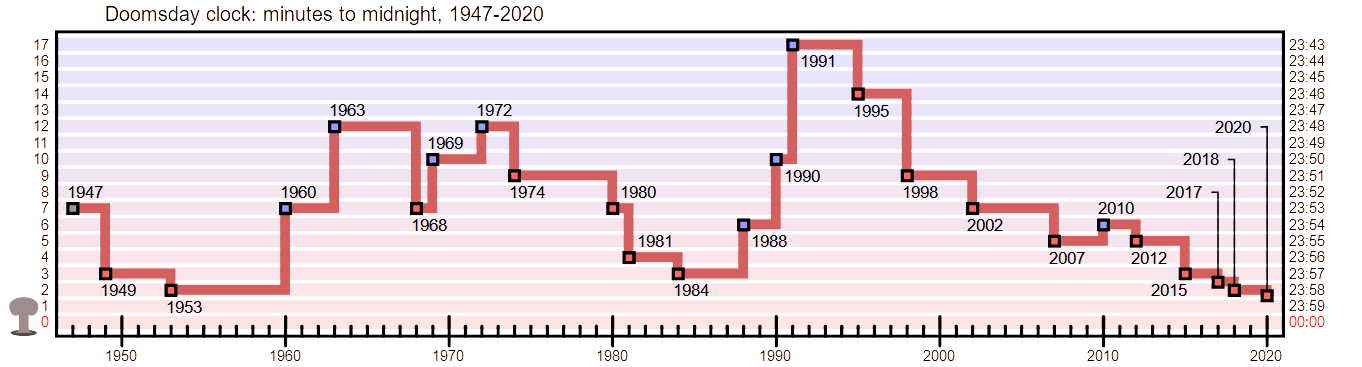
\includegraphics[width=0.95\linewidth]{images/Libro-img018.png}
  \caption{Di Fastfission 15:00, 14 April 2008 (UTC) - Opera
propria, Pubblico dominio, \raggedright\url{https://commons.wikimedia.org/w/index.php?curid=1575536}}
\end{figure}

\noindent \textbf{\large Overshoot Day} \\
L'Overshoot Day è il giorno in cui l'umanità ha consumato tutte le risorse naturali (inclusa la capacità di assorbire i nostri rifiuti, come l'anidride carbonica) che la Terra è in grado di rigenerare in un intero anno.

Nel 2019 l'overshoot day è stato il 29 luglio, questo vuol dire che per 5 mesi siamo stati in
debito con la terra e abbiamo utilizzato risorse che si sono accumulate molti anni fa quando riuscivamo ad essere in
credito col pianeta.

Questa data in realtà è peggio di quanto sembri, perché nel mondo ci sono paesi ad alto reddito occidentali con il loro tenore di vita e i
paesi a basso reddito con utilizzo di risorse molto inferiori alle nostre.

L'overshoot day dell'Europa nel 2019 è stato il 10 maggio e, per l'Italia il
15 maggio.

Come potete vedere da questo grafico l'ultima volta che siamo riusciti a consumare meno risorse di
quante ne siano state prodotte è stato il 1970, quando c'erano circa 3,7 miliardi di persone, da
allora il giorno si è avvicinato sempre di
più\endnote{\raggedright\url{https://www.overshootday.org/newsroom/press-release-july-2019-italian/} }.

Sul sito ufficiale potete calcolare il vostro personale overshoot day:

www.footprintcalculator.org 

e vedere l'impronta ecologica di ogni stato:

data.footprintnetwork.org

L’estinzione di specie, umana inclusa, non rappresenta un disallineamento intenzionale della natura, bensì l’esito di dinamiche ecologiche e selettive: se un organismo non trova più risorse, tende a scomparire, finché non si ristabilisce un nuovo equilibrio tra domanda e offerta ambientale.

Alcuni studi (IPCC e ricerche recenti) osservano che, se le emissioni non saranno drasticamente ridotte, entro il 2050 molte aree, soprattutto tropicali e subtropicali, potrebbero diventare difficile da abitare a causa di ondate di calore estremo, siccità o innalzamento del livello del mare\endnote{\raggedright\url{https://arxiv.org/abs/2212.04474}}. Questo ha portato alla nascita di alcuni movimenti come il no-fly, dove le persone rinunciano all'aereo come mezzo di trasporto preferendo il treno.

\needspace{4cm}
\begin{figure}[H]
  \centering
  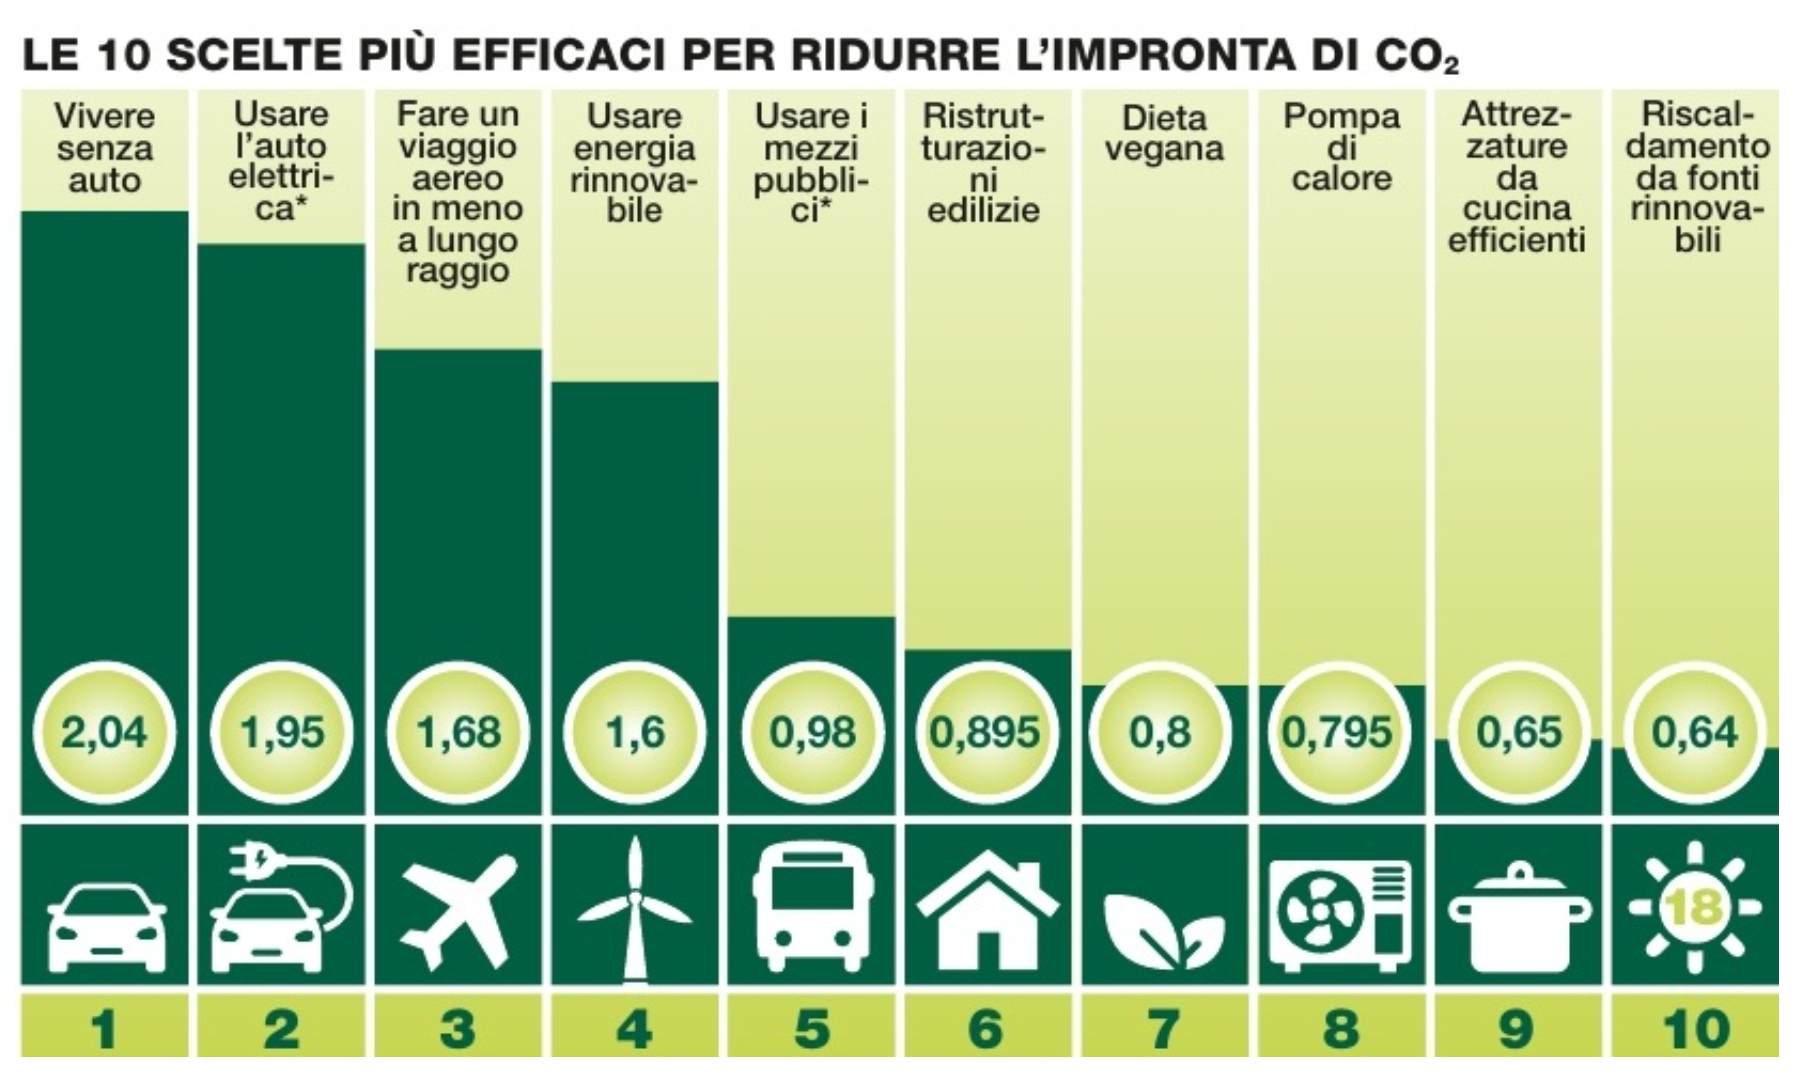
\includegraphics[width=0.95\linewidth]{images/Libro-img019.jpg}
  \caption{Tratto da un ritaglio di giornale (Focus)}
\end{figure}

\begin{table}[]
\begin{tabular}{lllll}
Mezzo di trasporto & Media di passeggeri & Emissioni (g CO2/(km * passeggeri) & & \\
Aeroplano & 88 & 285 & & \\
Nave & - & 245 & & \\
Grande macchina & 1,5 & 158 & & \\
Piccola Macchina & 1,5 & 104 & & \\
Moto & 1,2 & 72 & & \\
Pullman & 12,7 & 68 & & \\
Grande macchina & 4 & 55 & & \\
Piccola macchina & 4 & 42 & & \\
Treno & 156 & 14 & & \\
Bicicletta & 1 & 0 & & 
\end{tabular}
\end{table}

Le navi da crociera emettono ingenti quantità di CO2\endnote{\raggedright\url{https://en.wikipedia.org/wiki/Environmental\_impact\_of\_transport}} e altri inquinanti per passeggero/km, posizionandosi generalmente tra i mezzi di trasporto più impattanti, anche se in specifici scenari di altissimo carico e lunghi viaggi le emissioni pro capite possono avvicinarsi a quelle di auto o autobus.. A seguire il trasporto
su gomma, quindi macchine, furgoni, camion, bus ecc… dove il rapporto di C02 prodotta per chilometro è più efficiente rispetto a navi e aerei, ma per via della loro numerosità e tempo di utilizzo sono i mezzi di trasporto ad
oggi più inquinanti. Infine abbiamo il treno che si conferma, con un ampio margine, il mezzo più ecologico, anche
rispetto alle auto elettriche per via dell'elevato numero di passeggeri che un solo mezzo può
trasportare. 
La scelta del treno, riducendo le macchine in circolazione permette quindi la diminuzione di CO2 di ridurre il
traffico, aumentare la sicurezza stradale.

\noindent \textbf{\large Cambiamento climatico} \\
Una delle critiche al cambiamento climatico, portata avanti da alcune persone, che sostengono di sentire più freddo rispetto ad anni fa. 
Meno 33 gradi a Chicago, meno 35 gradi in Nord
Dakota con venti freddi a meno 52 gradi. Questo dipende da diversi fattori, il primo è confondere il meteo con il clima. Il meteo fa riferimento ad un tempo e uno spazio limitato. Mentre il clima si riferisce a tempi più lunghi,
nell'ordine di 150 anni e globalmente. Un altro motivo, che spiega questi fenomeni è il vortice polare, che possiamo vederlo come
un anello di venti freddi che ruota attorno al Polo Nord. Con il surriscaldamento terreste, questo vortice è diventato
irregolare, disegnando onde più ampie in alcune aree e più ristrette in altre. Nei punti più ampi verranno quindi
coinvolte dal freddo aree dove solitamente il clima è più mite. 

Negli ultimi 70 anni alcuni scienziati hanno osservato che il clima si sta raffreddando, ma il resto della comunità
scientifica non si è ritrovata con questi dati, infatti 13 dei 14 anni più caldi si sono verificati proprio nel
ventunesimo secolo. Considerare solo la temperatura può essere fuorviante, abbiamo altri indici come lo scioglimento
dei ghiacci, l'innalzamento dei mari. Anche questi dati possono essere travisati. Possiamo sostenere che negli ultimi anni i ghiacci sono aumentati del 40\%. Questa non sarebbe una notizia falsa, ma decontestualizzata. Come possiamo vedere dal seguente grafico, l'estensione del ghiaccio ha un andamento altalenante, ma la tendenza è comunque a calare.

\needspace{4cm}
\begin{figure}[H]
  \centering
  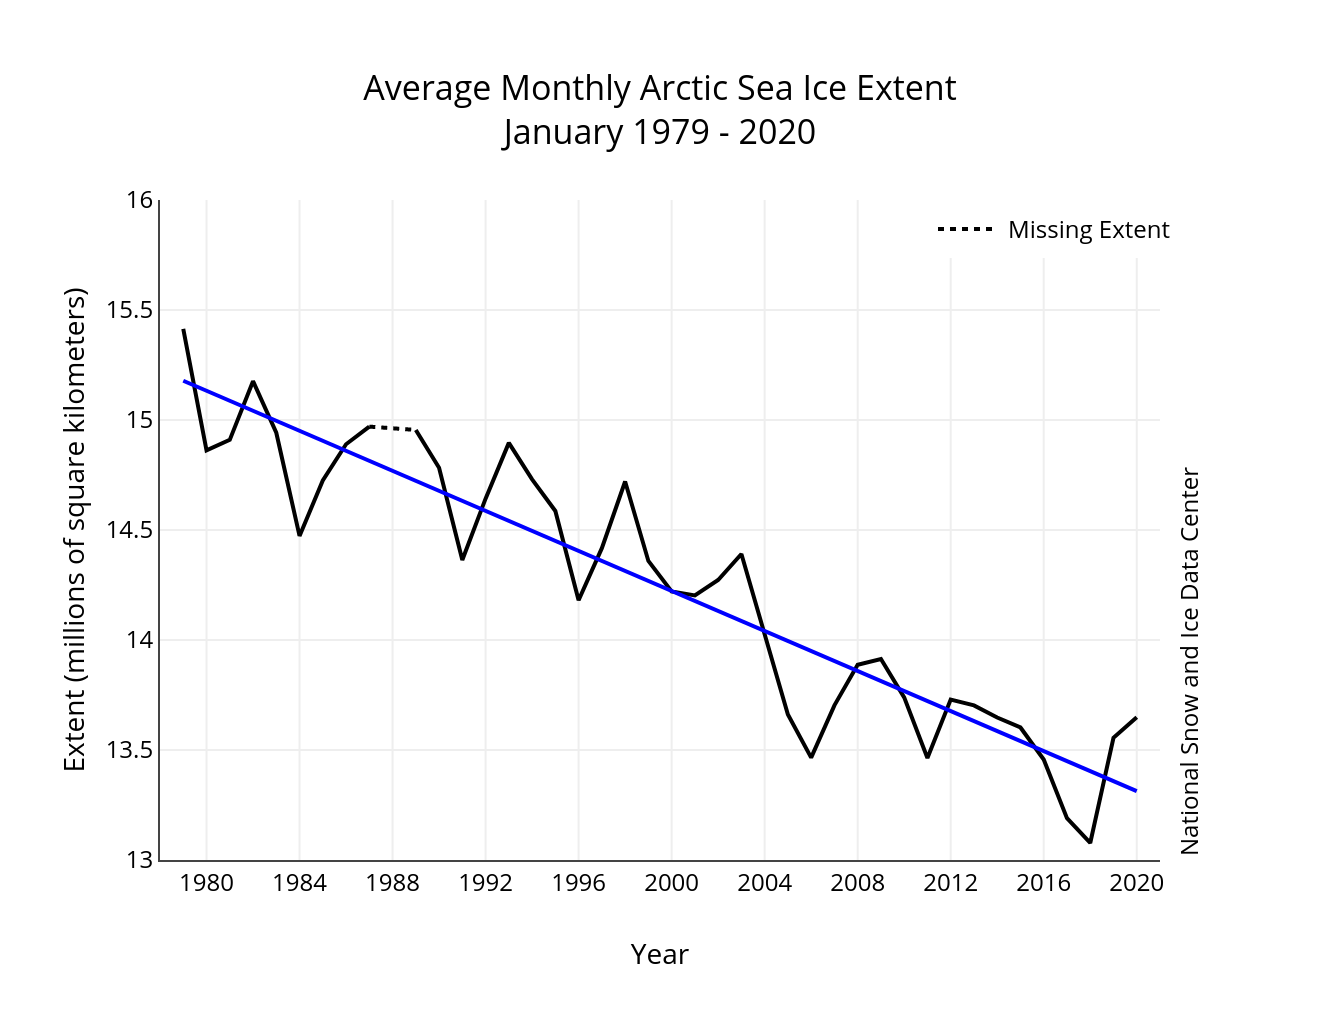
\includegraphics[width=0.95\linewidth]{images/Libro-img021.png}
  \caption{L'estensione mensile del ghiaccio di gennaio per il
periodo 1979-2020 mostra un calo del 3,15 percento per decennio. Credits: \href{https://nsidc.org/arcticseaicenews/2020/02/}{National Snow and Ice Data Center}}
\end{figure}

Il modo più giusto di guardare questo grafico è quindi la linea blu e non l'ultimo pezzo di linea nera. Questo genere di lettura viene fatta su qualsiasi cosa, è un'arma molto usata in molte forme di negazionismo, fake news e complotti.

Il maggiore responsabile del surriscaldamento globale è la CO2, di cui però sappiamo che gli esseri umani sono responsabili della
produzione di sole 30 gigatonnellate rispetto alle 780 emesse dall'oceano e dal
terreno. Il pianeta terra ha però le risorse per riassorbire queste 780 gigatonnellate a patto che ci siano sufficienti
piante. Per questo motivo si sente spesso parlare del problema della deforestazione, oltre ad altri problemi che porta
con se, come la riduzione di biodiversità vegetale e animale, che a cascata fa sparire altre specie utili alla nostra
sopravvivenza. Secondo lo studio “Deforestation and world population sustainability: a quantitative
analysis”\endnote{\raggedright\url{https://www.nature.com/articles/s41598-020-63657-6}} , pubblicato a maggio 2020 su Scientific
Reports di Nature, il ritmo attuale della deforestazione, se mantenuto, potrebbe compromettere seriamente la capacità della Terra di sostenere l'attuale popolazione umana entro i prossimi 20-40 anni, portando a scenari critici di collasso demografico.

La CO2 porta a diversi effetti a catena. L'aumento della temperatura provoca una maggiore evaporazione dell'acqua, che forma più nuvole. Il ruolo delle nuvole nel bilancio energetico è complesso: possono contribuire all'effetto serra intrappolando il calore, ma possono anche riflettere la luce solare nello spazio. Tuttavia, l'effetto serra in generale è il fenomeno per cui alcuni gas nell'atmosfera intrappolano il calore riflesso dalla Terra, impedendogli di disperdersi nello spazio e causando un ulteriore aumento della temperatura.

\clearpage
\noindent \textbf{\large Dieta} \\

\begin{wraptable}{r}{6cm}
\centering
\caption{\raggedright\url{https://it.wikipedia.org/wiki/Impatto\_ambientale\_dell\%27industria\_dei\_cibi\_animali}}
\begin{tabular}{|m{3cm}|m{2cm}|}
\hline
Alimento &
Impronta idrica (in litri per kg)\\\hline
carne di manzo &
15 400\\\hline
carne di pecora &
10 400\\\hline
carne di maiale &
5990\\\hline
burro &
5550\\\hline
carne di capra &
5520\\\hline
formaggio &
5060\\\hline
carne di pollo &
4330\\\hline
uova &
3300\\\hline
riso &
2500\\\hline
soia &
2145\\\hline
pasta &
1850\\\hline
pane &
1608\\\hline
grano &
1827\\\hline
mais &
1220\\\hline
latte di mucca (1 litro) &
1020\\\hline
tè (1 litro) &
480\\\hline
cetriolo &
350\\\hline
zucca &
350\\\hline
patate &
290\\\hline
cavolo &
280\\\hline
lattuga &
240\\\hline
pomodori &
200\\\hline
\end{tabular}
\end{wraptable}

Cosa centra la dieta con il cambiamento climatico? Quello della sostenibilità alimentare è un problema molto complesso che cercheremo di osservare attraverso alcuni grafici e tabelle, come quella qui a fianco. Per le principali famiglie di alimenti possiamo conoscere l'impatto idrico, di CO2, sulla deforestazione ecc... In che modo un alimento può avere un impatto ambientale? L'atto di mangiare non inquina, ma il modo in cui vengono prodotti gli alimenti potrebbe. Alcuni alimenti hanno bisogno di diversi passaggi industriali con macchinari che hanno un consumo elevato, questi cibi sono definiti processati, ma non riguarda solo questa tipologia. Come possiamo notare dalla tabella qui a fianco sull'impronta idrica, ma anche nei successivi grafici, la carne, soprattutto quella di bovino, copre le prime posizioni. Gli animali possiamo vederli come dei sistemi, di solito più sono grossi e meno sono efficienti. Per allevare gli animali serve cibo che prendiamo dai campi. Immaginate quanti chili di cibo mangia una mucca prima di essere macellata e soprattutto quanti litri d'acqua beve. La produzione di 1kg di carne di manzo comporta circa 15500 litri (94\% di ‘green water’ che non incide direttamente sui bacini idrici) e tra 300–1300 litri di acqua blu e grigia utilizzata). Ora immaginate di essere in una stanza e di avere da una parte
la nostra mucca macellata e dall'altra parte tutto quello che la mucca ha mangiato e bevuto durante la sua vita.
Se si dovesse scegliere tra consumare la carne della mucca o le risorse vegetali che essa ha impiegato per crescere, la logica dell'efficienza energetica suggerisce che le risorse vegetali dirette potrebbero sostenere un maggior numero di individui o per un periodo più lungo, data l'inefficienza della conversione energetica dalla biomassa vegetale a quella animale.

Quando una mucca mangia, convertirà una piccola parte di quel cibo in carne (3-5\%) e, il resto viene trasformato in peli, corna, ossa, zoccoli, sangue, gas, calore, movimento ecc...

Potremmo pensare che evitare la carne, possa impattare solo in minima parte sull'inquinamento globale, ma attualmente il 12-18\% delle emissioni di gas serra provengono da allevamenti animali\endnote{\raggedright\url{https://it.wikipedia.org/wiki/Impatto\_ambientale\_dell\%27industria\_dei\_cibi\_animali}}
(una buona parte prodotta anche dai gas intestinali e feci), e occorrono 15.500 litri di acqua per produrre 1 kg di carne di manzo, mentre per coltivare un chilo di grano servono tra i 500 e i 4mila litri.

\clearpage

\begin{wraptable}{l}{7.855cm}
\centering
\caption{\raggedright\url{https://it.wikipedia.org/wiki/Impatto\_ambientale\_dell\%27industria\_dei\_cibi\_animali}}
\begin{tabular}{|m{3.575cm}|m{3.576cm}|}
\hline
\multicolumn{2}{|m{7.3510003cm}|}{Cause di deforestazione dell'Amazzonia brasiliana}\\\hline
Pascolo del bestiame  &
65-70\%\\\hline
Agricoltura su piccola scala &
20-25\%\\\hline
Agricoltura su larga scala &
5-10\%\\\hline
Taglio del legname &
2-3\%\\\hline
Altro &
1-2\%\\\hline
\end{tabular}
\end{wraptable}

Bojana Bajzelj professoressa di ingegneria a Cambridge osservò che l'efficienza media di un allevamento che converte
del foraggio vegetale in carne è meno del 3\%, e più carne mangiamo, più terre coltivabili vengono utilizzate
per produrre risorse alimentari per gli animali che forniscono carne per gli umani. 
Se coltivassimo un terreno con la soia produrremmo il 314\%\endnote{\raggedright\url{https://humaneherald.org/wp-content/uploads/2019/05/calories-and-protein-produced-per-acre-1.pdf}} di proteine in più rispetto alla carne di pollo e 1800\%\endnote{\raggedright\url{https://faunalytics.org/alternative-protein-production-counting-the-calories/}} in più rispetto alla carne bovina.
Attualmente siamo 8 miliardi ma stiamo coltivando proteine per sfamarne 10 miliardi, solo che più della metà è
destinata agli animali negli allevamenti\endnote{Fonte: World Bank}. La produzione di carne è anche il principale
fattore della deforestazione, sia per far pascolare il bestiame sia per creare coltivazioni per sfamarlo.

Di seguito un grafico che mostra le emissioni di CO2 per grammo di proteine. Vediamo Quindi come un grammo di carne
bovina emetta molta più CO2 rispetto a grano, mais e legumi. 

Fagioli, verdure (non coltivate in serra) e, alcuni pesci allevati in modo sostenibile, hanno un
rapporto vantaggioso tra salute e costi ambientali. Sono in pari invece alimenti come latte, yogurt, uova, e le verdure
coltivate in serra. Mentre svantaggiosi gli alimenti come carne di manzo, carni lavorate, maiale e agnello, che hanno
mostrato elevati costi sanitari e ambientali. Una porzione da circa 200g di carne bovina equivalgono a ~4–6kg CO2-eq, corrispondenti a un’automobile media per 20km!

\needspace{4cm}
\begin{figure}[H]
\centering
\begin{tikzpicture}
\begin{axis}[
    xbar, xmin=0,
    width=12cm, enlarge y limits=0.5,
    xlabel={Emissioni (kg CO2-eq per kg di prodotto)},
    symbolic y coords={Legumi, Mais, Grano, Radici Amidacee, Uova, Pesca non a strascico, Latteria, Pollame, Maiale, Acquacoltura non a ricircolo,Pesca a strascico, Acquacoltura a ricircolo, Carne Di Ruminanti},
    ytick=data,
    nodes near coords, nodes near coords align={horizontal},
    ]
\addplot coordinates {(0.25,Legumi) (1.2,Mais) (1.2,Grano) (1.7,Radici Amidacee) (6.8,Uova) (8.6,Pesca non a strascico) (9.1,Latteria) (10,Pollame) (10,Maiale) (12,Acquacoltura non a ricircolo) (26,Pesca a strascico) (30,Acquacoltura a ricircolo) (62,Carne Di Ruminanti)};
\end{axis}
\end{tikzpicture}
\caption{Emissioni medie di gas a effetto serra per i diversi tipi di alimenti espressi in g di CO2-Ceq per g di proteine}
\end{figure}

Quindi è meglio diventare vegani, vegetariani o rimanere onnivori dal punto di vista ambientale?

Molti hanno trattato questo fenomeno, dal
Guardian\endnote{\raggedright\url{https://www.theguardian.com/lifeandstyle/2010/jul/18/vegetarianism-save-planet-environment} }
all'Onu\endnote{\raggedright\url{http://www.unep.org/resourcepanel/Portals/24102/PDFs/PriorityProductsAndMaterials\_Report.pdf}
} che da uno studio del 2010 sostiene che allontanandosi dai prodotti animali si otterrebbe un sostanziale cambiamento
sugli effetti ambientali.

In una ricerca\endnote{\raggedright\url{https://now.tufts.edu/news-releases/us-land-capacity-feeding-people-could-expand-dietary-changes}
} pubblicata lo scorso luglio sulla rivista Elementa, un team di scienziati della Friedman School of Nutrition Science
and Policy della Tufts University ha analizzato dieci diverse diete - dall'alimentazione americana media attuale, a una
dieta onnivora, a una puramente vegana - e ha stabilito quale di queste permetterebbe di sfamare più persone con lo
sfruttamento dei terreni agricoli degli Stati Uniti. La dieta peggiore è risultata quella americana ricca di carne,
grassi e dolcificanti, circa l'80\% delle terre coltivabili è utilizzata per cibo animale, la
migliore, a sorpresa, quella vegetariana e non vegana. La motivazione è che i terreni adibiti all'allevamento, se gestiti in modo non sostenibile, possono degradarsi e perdere fertilità nel tempo, rendendo difficile o impossibile la coltivazione successiva di ortaggi o piante da frutto senza interventi significativi di ripristino.

Fortunatamente una dieta vegetariana è possibile facilmente senza squilibri alimentari se fatta nel modo corretto, a dispetto di quella vegana dove bisogna stare più attenti.
Alcuni studi epidemiologici stimano che una parte delle morti per tumori o malattie cardiovascolari (alcune percentuali limitate) sia attribuibile all’eccessivo consumo di carne rossa. Queste analisi suggeriscono inoltre potenziali risparmi nei costi sanitari.
Il mio intento non è quello di farvi diventare vegetariani, infatti, se riuscissimo a rimuovere o anche solo a ridurre la carne di manzo, come abbiamo visto dai precedenti grafici, riusciremmo a ridurre già moltissimo sull'ambiente, anche senza rinunciare a tutta la carne.
Anche le nuove alternative come la carne coltivata in laboratorio o i grilli, per quanto siano promettenti, ad oggi hanno un efficienza non troppo differente da quella del pollo.

\needspace{4cm}
\begin{wrapfigure}{i}{9cm}
  \centering
  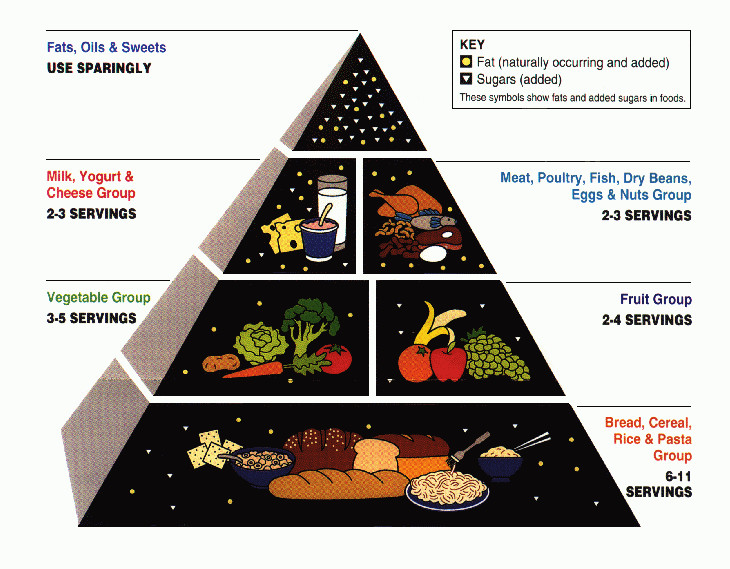
\includegraphics[width=0.95\linewidth]{images/Libro-img059.jpg}
  \begin{minipage}{\linewidth}
    \caption{By The food pyramid, from http://www.nal.usda.gov/fnic/Fpyr/pyramid.gif, Public Domain,
\raggedright\url{https://commons.wikimedia.org/w/index.php?curid=680809}}
  \end{minipage}
\end{wrapfigure}

Un ulteriore fortuna vuole che le diete più sane, sono anche quelle che hanno un minore impatto ambientale, come possiamo notare nella piramide
alimentare c'è molta frutta e verdura, oltre a suggerire di evitare cibi elaborati, insaccati e salumi, dichiarati cancerogeni
dall'OMS\endnote{\raggedright\url{http://www.thelancet.com/journals/lanonc/article/PIIS1470-2045\%2815\%2900444-1/fulltext}} e ridurre la carne rossa, massimo due porzioni a settimana. Secondo uno studio dell'Università del Michigan, attraverso modelli di valutazione dell'impatto sulla salute, si è stimato che il consumo di un solo hot dog potrebbe essere associato a una perdita di circa 36 minuti di vita in salute. I calcoli hanno evidenziato che, negli USA, il consumo di ogni grammo di carne lavorata potrebbe comportare una diminuzione proporzionale di secondi di vita in salute.

\needspace{4cm}
Di seguito possiamo vedere quanto viene consumato un certo alimento nelle varie aree del mondo e quanto invece andrebbe
consumato (dieta di riferimento) rappresentato dalla linea
tratteggiata\endnote{\raggedright\url{https://www.semanticscholar.org/paper/Faculty-Opinions-recommendation-of-Food-in-the-the-Symonds/8826b114812333f7b154b6d8a1886a66ed09da31\#paper-header}}. La carne rossa nel nord America supera il 600\% del consumo consigliato.

\begin{figure}[H]
  \begin{minipage}{17cm}
    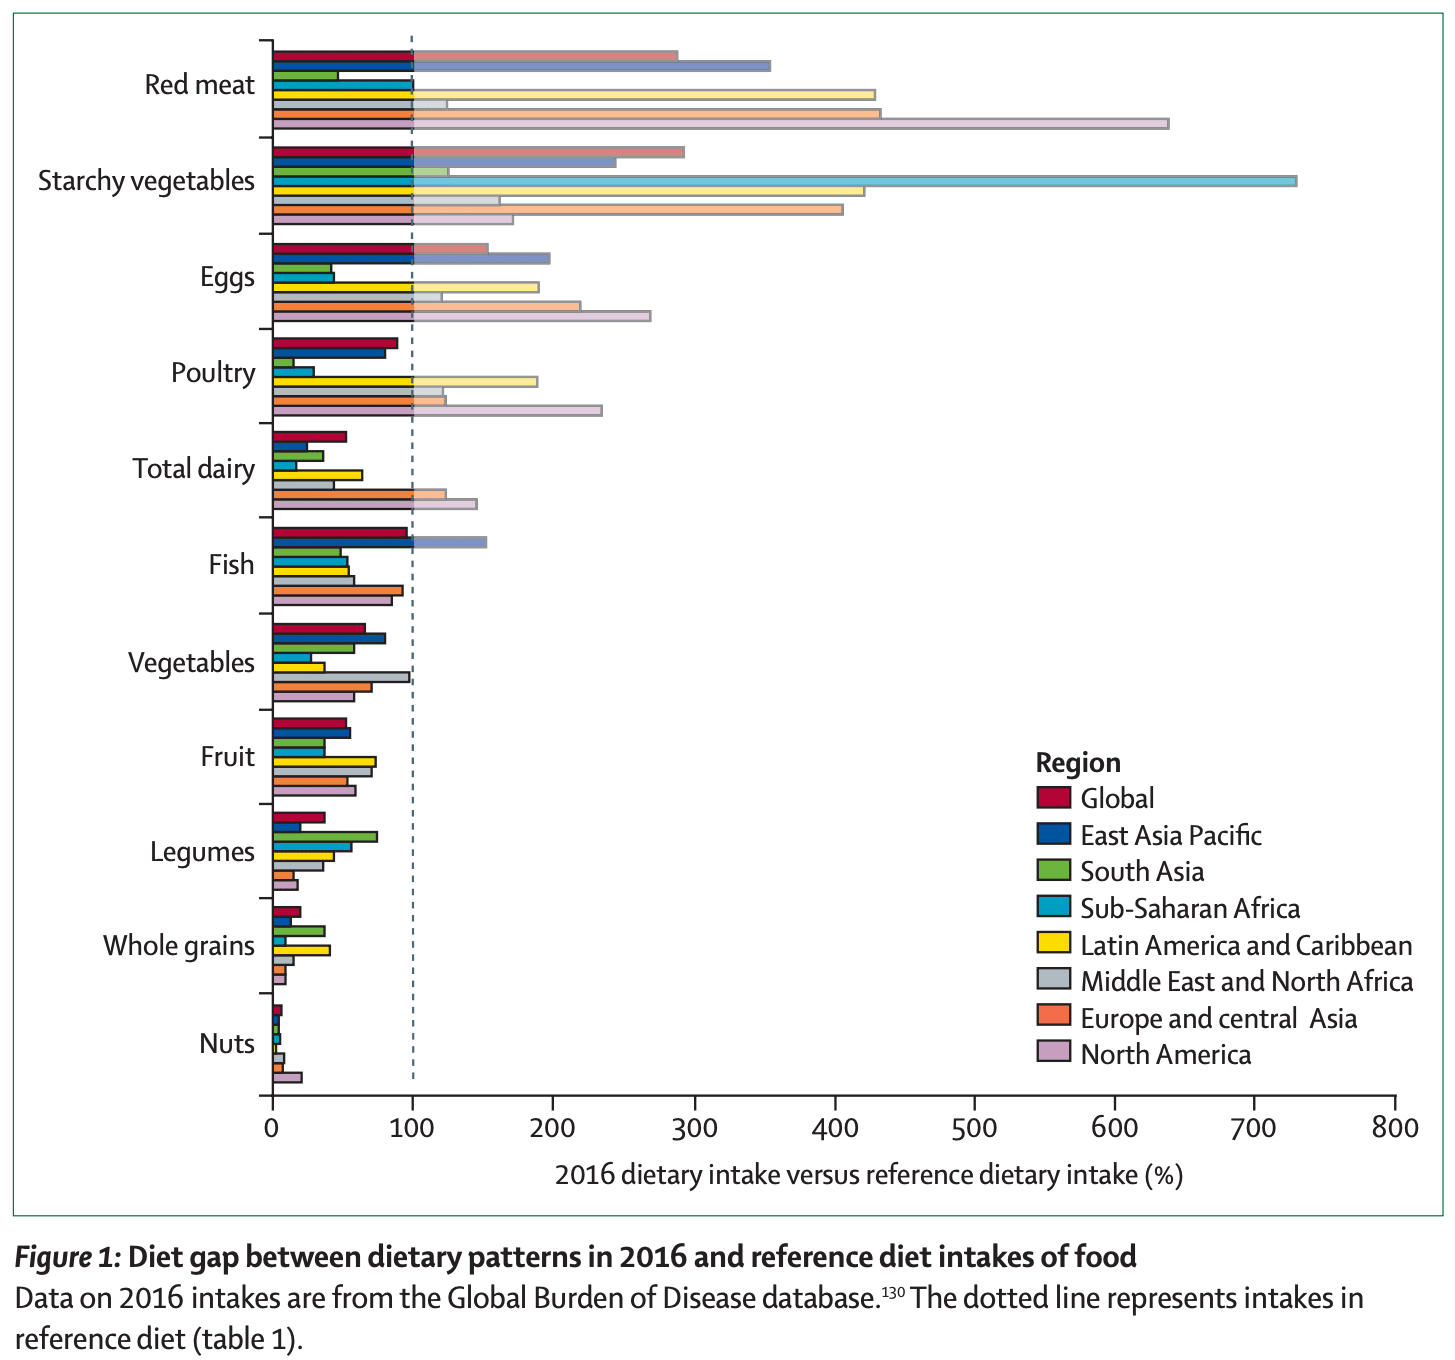
\includegraphics[width=17cm]{images/Libro-img023.png}
    \caption{Sull'asse Y, leggendo dall'alto verso il basso troviamo, carne rossa, verdure
amidacee, uova, pollame, latticini, pesce, vegetali, frutta, legum, cereali integrali, noccioline. 
Nella legenda troviamo: Globale, Asia dell'est, Sud Asia, Africa subsahariana, America latina e Caraibi, nord Africa e Medio Oriente, Europa e Asia centrale, nord America }
  \end{minipage}
\end{figure}

In alternativa al vegetarianesimo sono nate alcune alternative

\begin{itemize}
\item Mangiare gli “invasori”: Ci sono alcune specie aliene, ovvero che non sono originarie di un certo luogo, come
per esempio la nutria o il pesce siluro in Italia, che sono stati importati da altri paesi. Queste specie, non
trovando predatori naturali si stanno moltiplicando, diventando un problema per altre specie animali, vegetali e
per l'ecosistema in generale. Seppur ogni creatura meriti di vivere, la proliferazione di questi animali invasivi spesso comporta un impatto devastante sugli ecosistemi e sulla biodiversità locale. Tuttavia, è importante notare che l'effettivo bilancio netto positivo in termini di vite salvate e impatti sull'ecosistema, derivante dal consumo di queste specie, è un ambito che richiede ulteriori evidenze e studi approfonditi. Per saperne di più potete visitare eattheinvaders.org
\item Reducetariani e flexitariani: Alternative al vegetarianesimo dove entrambe si impegnano a ridurre il consumo di carne, i primi per l'ambiente e i secondi per la propria salute. In realtà la maggioranza delle persone che si identificano come vegetariane sono reducetariani o flexitariani, in quanto può capitare che durante l'anno consumino carne. Purtroppo, per anni, alcune forme di promozione del messaggio vegetariano e vegano hanno adottato toni giudicanti, implicando che 'voi siete sbagliati e dovreste vergognarvi mentre noi siamo buoni'. Questo ha contribuito a creare un certo imbarazzo o diffidenza quando qualcuno si definisce vegetariano, anche se si chiarisce che non è intenzione giudicare le scelte alimentari altrui. Con il termine reducetariano rimuoviamo questo
linea così netta tra un gruppo e l'altro, risultando più inclusivo. Talmente inclusivo che tutti
possiamo diventare reducetariani. Se tutti noi seguissimo una dieta del “lunedì senza carne”, astenendoci dal mangiare
carne ogni lunedì, avremmo un miliardo di vegetariani in più dall'oggi al domani, con ciò che questo comporta come impatto ambientale.
\end{itemize}

\begin{mdframed}[linewidth=1pt]
Anche l'attuale eccesso di cibi processati, di igiene, di farmaci, soprattutto antibiotici, assunti
direttamente o indirettamente tramite una dieta di carne contribuiscono a danneggiare un'utile popolazione
del nostro intestino, il microbiota. Un microbiota indebolito da un ambiente eccessivamente pulito e
dall'utilizzo massivo di antibiotici potrebbe essere una delle cause della grande diffusione di
allergie degli ultimi decenni. La letteratura evidenzia infatti come il nostro sistema immunitario diventi davvero
efficiente se fin dalla nascita si viene a contatto con una quantità sufficiente di germi e parassiti. 
\end{mdframed}

\needspace{4cm}
\noindent \textbf{\large Cosa si può fare?} \\

\begin{wrapfigure}{i}{9cm}
  \centering
  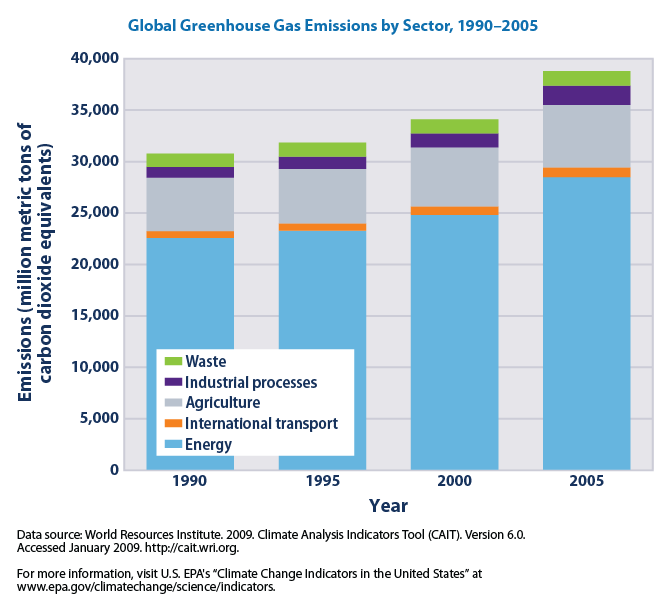
\includegraphics[width=0.95\linewidth]{images/Libro-img024.png}
  \begin{minipage}{\linewidth}
    \caption{Legenda tradotta: Rifiuti, processi industriali,
agricoltura, trasporti internazionali e energia. 
Credits: By US Environmental Protection Agency - Climate Change Indicators in the United States: Figure 2. Global
Greenhouse Gas Emissions by Sector, 1990-2005. Page 12 of PDF. Published 2010., Public Domain,
\raggedright\url{https://commons.wikimedia.org/w/index.php?curid=20445607} }
  \end{minipage}
\end{wrapfigure}

Per riuscire in questa sfida ecologica siamo chiamati a fare dei cambiamenti individuali, come l'alimentazione, riciclare, prestare attenzione ai modi che utilizziamo per spostarci
ecc… Le scelte più importanti che possono abbassare il nostro impatto ambientale, non comportano necessariamente una riduzione del tenore di
vita, ma un cambiamento. L'importanza di queste scelte non vanno viste soltanto per preservare il
pianeta del futuro, di quando non ci saremo più, ma anche per quello attuale. In Europa un decesso su otto è dovuto
all'inquinamento\endnote{\raggedright\url{https://it.euronews.com/my-europe/2020/09/08/europa-un-cittadino-su-8-muore-per-inquinamento-e-fattori-ambientali}}. 
A volte può risultare difficile fare cambiamenti che possano ridurre le proprie emissioni, ma possiamo
riassorbirle. Ci sono siti come Treedom, ZeroCO2 e Ecosia che tra le varie cose permettono, di farci piantare alberi in
giro per il mondo. Alcune campagne promuovono l’uso di progetti di riforestazione o tecnologie di cattura del carbonio, ma queste andrebbero considerate complementari, non sostitutive, rispetto alla riduzione delle emissioni alla fonte. 
Secondo il database ‘Carbon Majors’ (CDP), 100 aziende fossili hanno generato il 71\% delle emissioni industriali cumulative nel periodo 1988‑2015, considerando le emissioni scope 1‑3\endnote{\raggedright\url{https://www.theguardian.com/sustainable-business/2017/jul/10/100-fossil-fuel-companies-investors-responsible-71-global-emissions-cdp-study-climate-change}}. Cosa producono queste aziende? Principalmente energia bruciando combustibili fossili, carbone, petrolio. La
produzione di energia è infatti il settore principalmente responsabile nell'emissione di gas
serra, come possiamo vedere nel grafico qui a fianco.

\needspace{4cm}
\begin{figure}[H]
  \centering
  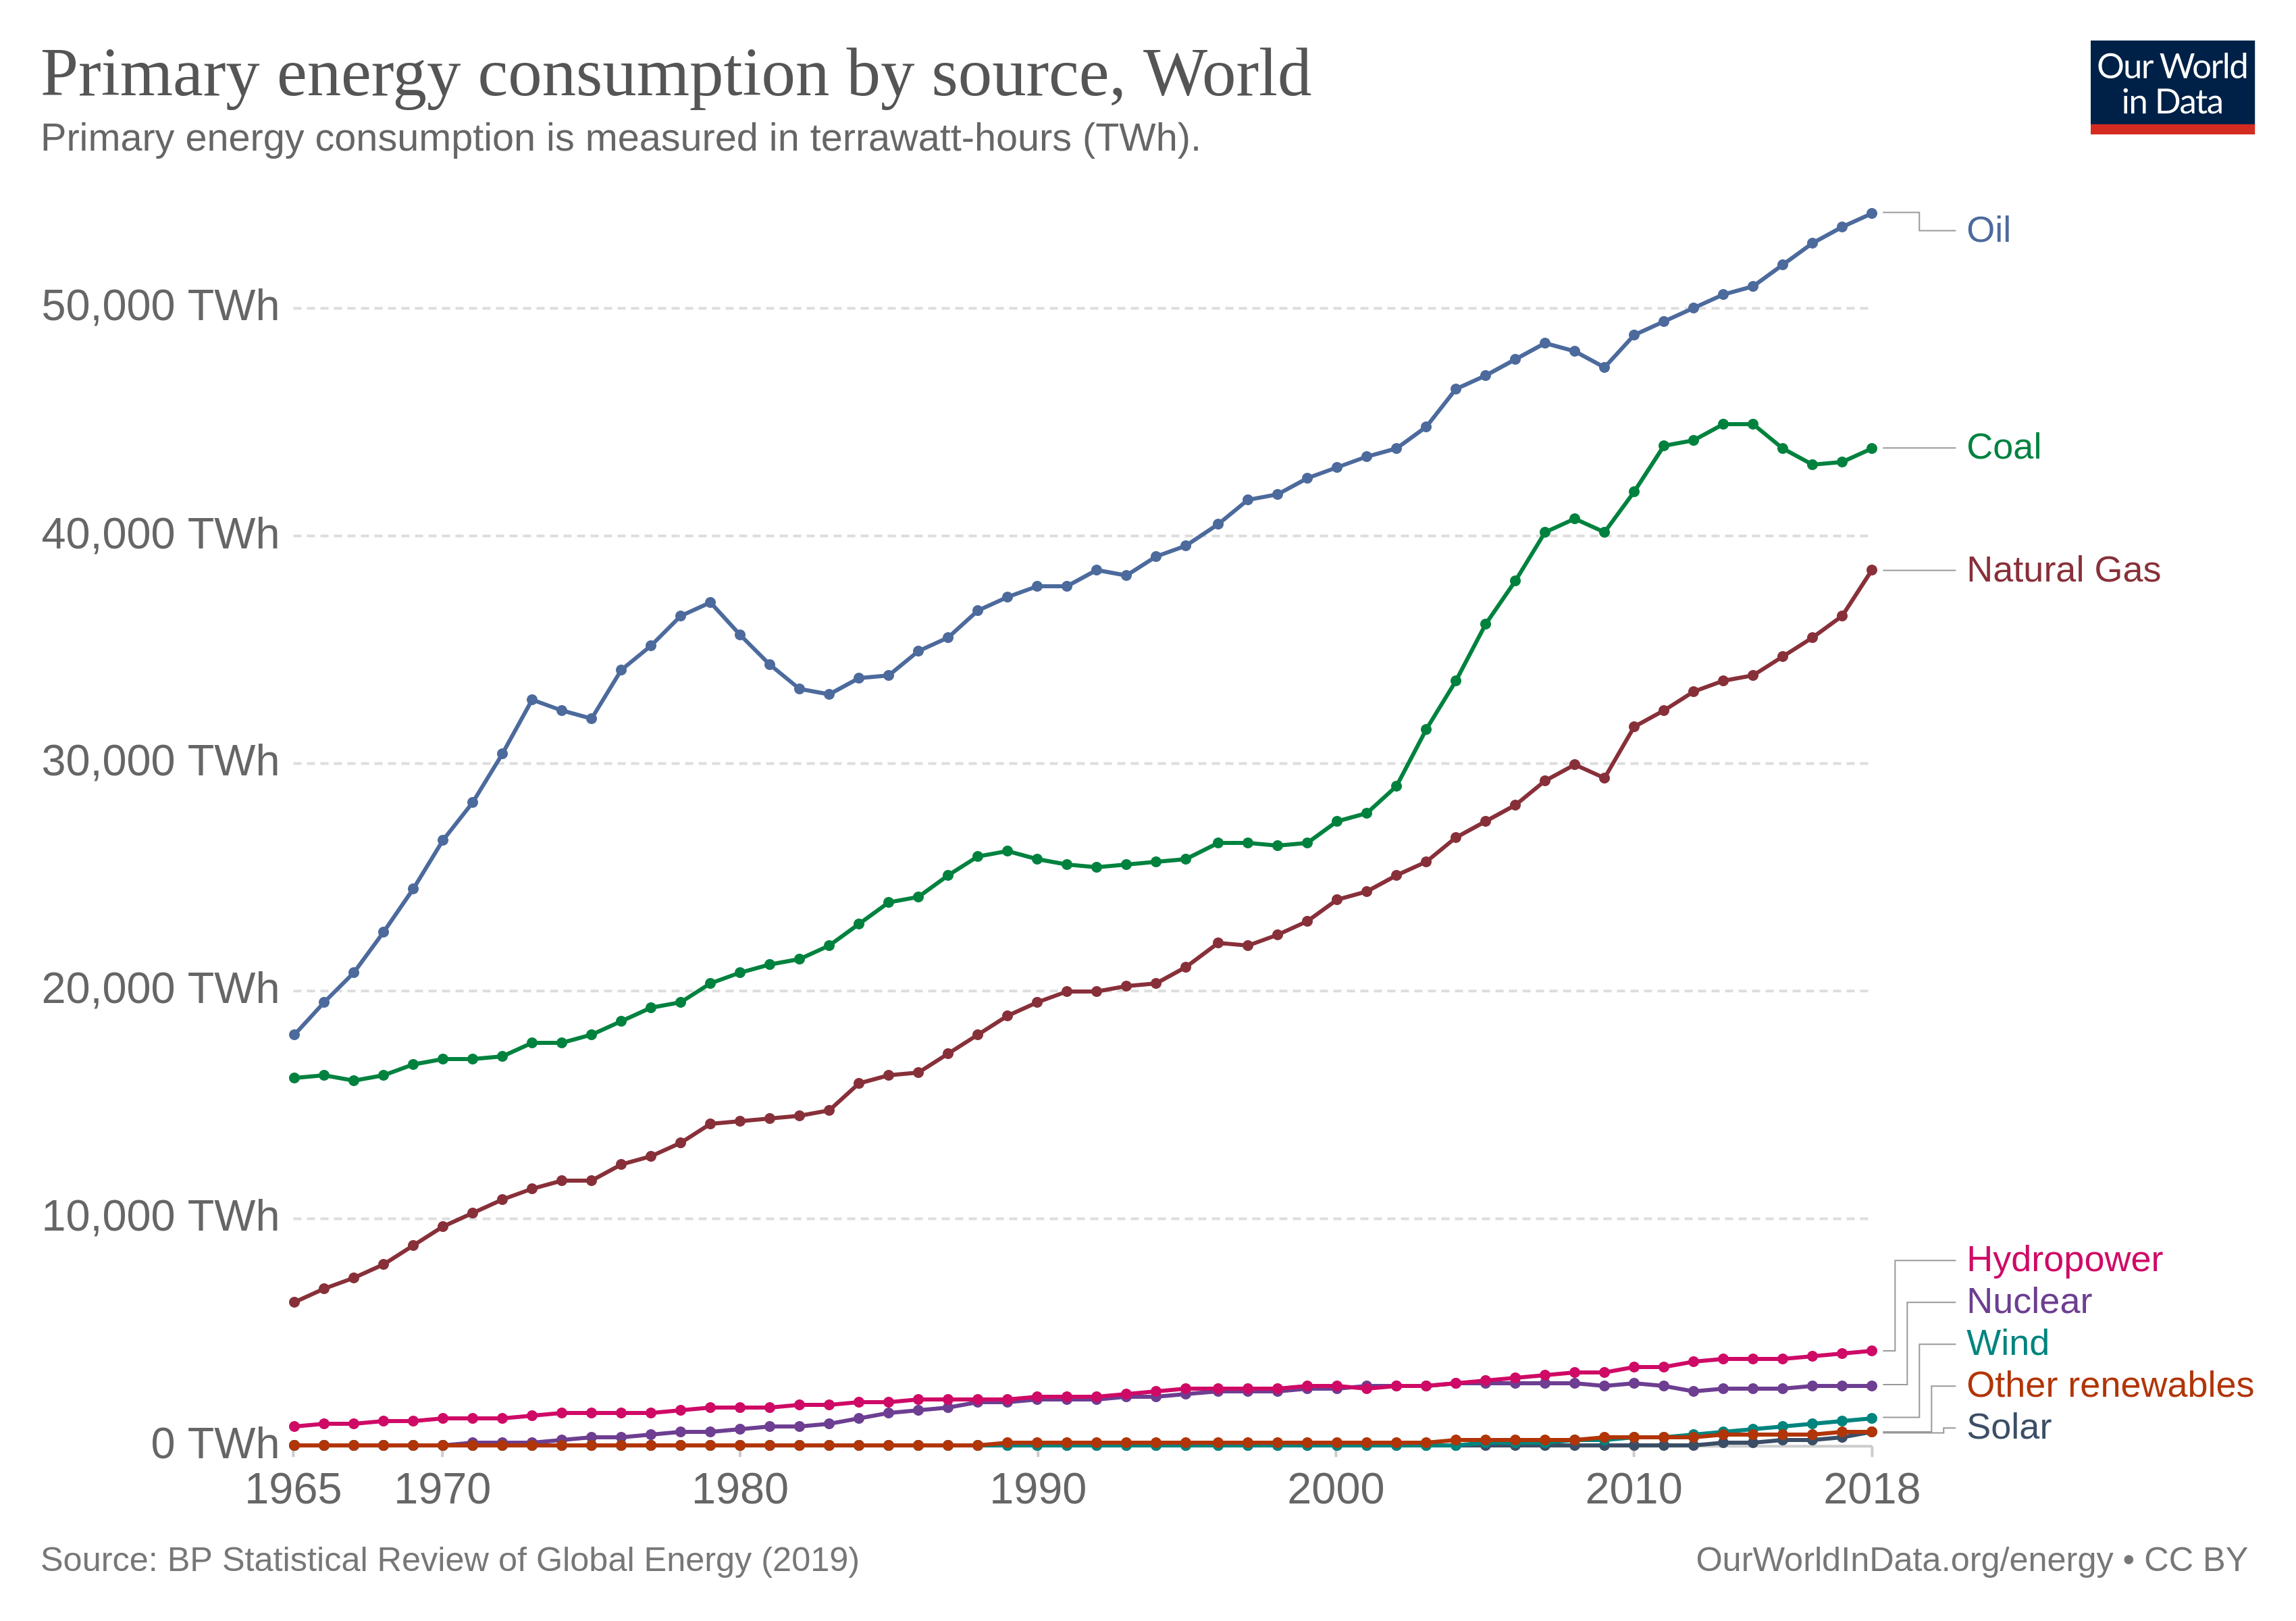
\includegraphics[width=0.95\linewidth]{images/Libro-img025.png}
  \caption{Dall'alto verso il basso: Petrolio, carbone, gas naturale, idroelettrico, nucleare, eolico, altro e solare
  Credits: \raggedright\url{https://ourworldindata.org/energy} }
\end{figure}

Seppur l'impiego di carbone, petrolio e gas naturali per la produzione energetica non siano più
metodi all'avanguardia, sono ancora molto diffusi. Potremmo essere portati a pensare che comprando
una macchina elettrica e scaldando casa con l'elettricità il grosso
dell'energia che utilizzeremo sarà pulita. Questo però dipende in realtà da come viene prodotta la
corrente, infatti ad oggi, l'energia elettrica viene prodotta principalmente da carbone e gas
naturale. Nel grafico a torta qui a fianco possiamo vedere la situazione mondiale, ma anche in Italia, come riportato
dal Wwf\endnote{\raggedright\url{https://www.wwf.it/il\_pianeta/clima\_ed\_energia/fermiamo\_il\_carbone/}}
l'11,6\% della produzione elettrica deriva dal carbone mentre troppe centrali termoelettriche
lavorano per un terzo della loro potenzialità. In Italia possiamo generare una potenza doppia al picco massimo mai
raggiunto, per cui potremmo chiudere o convertire in centrali green tutte quelle più inquinanti. Quindi scegliere di
scaldare casa con una pompa di calore e comprare una macchina elettrica è può essere una buona idea se il vostro
fornitore di corrente la produce tramite fonti rinnovabili. Questo è un esempio di scelta che non impatta sul nostro
tenore di vita. Anche in Italia abbiamo fornitori che producono corrente al 100\% da fonti rinnovabili e il prezzo è lo
stesso di fornitori che utilizzano combustibili fossili.

\needspace{4cm}
\begin{figure}[H]
  \centering
  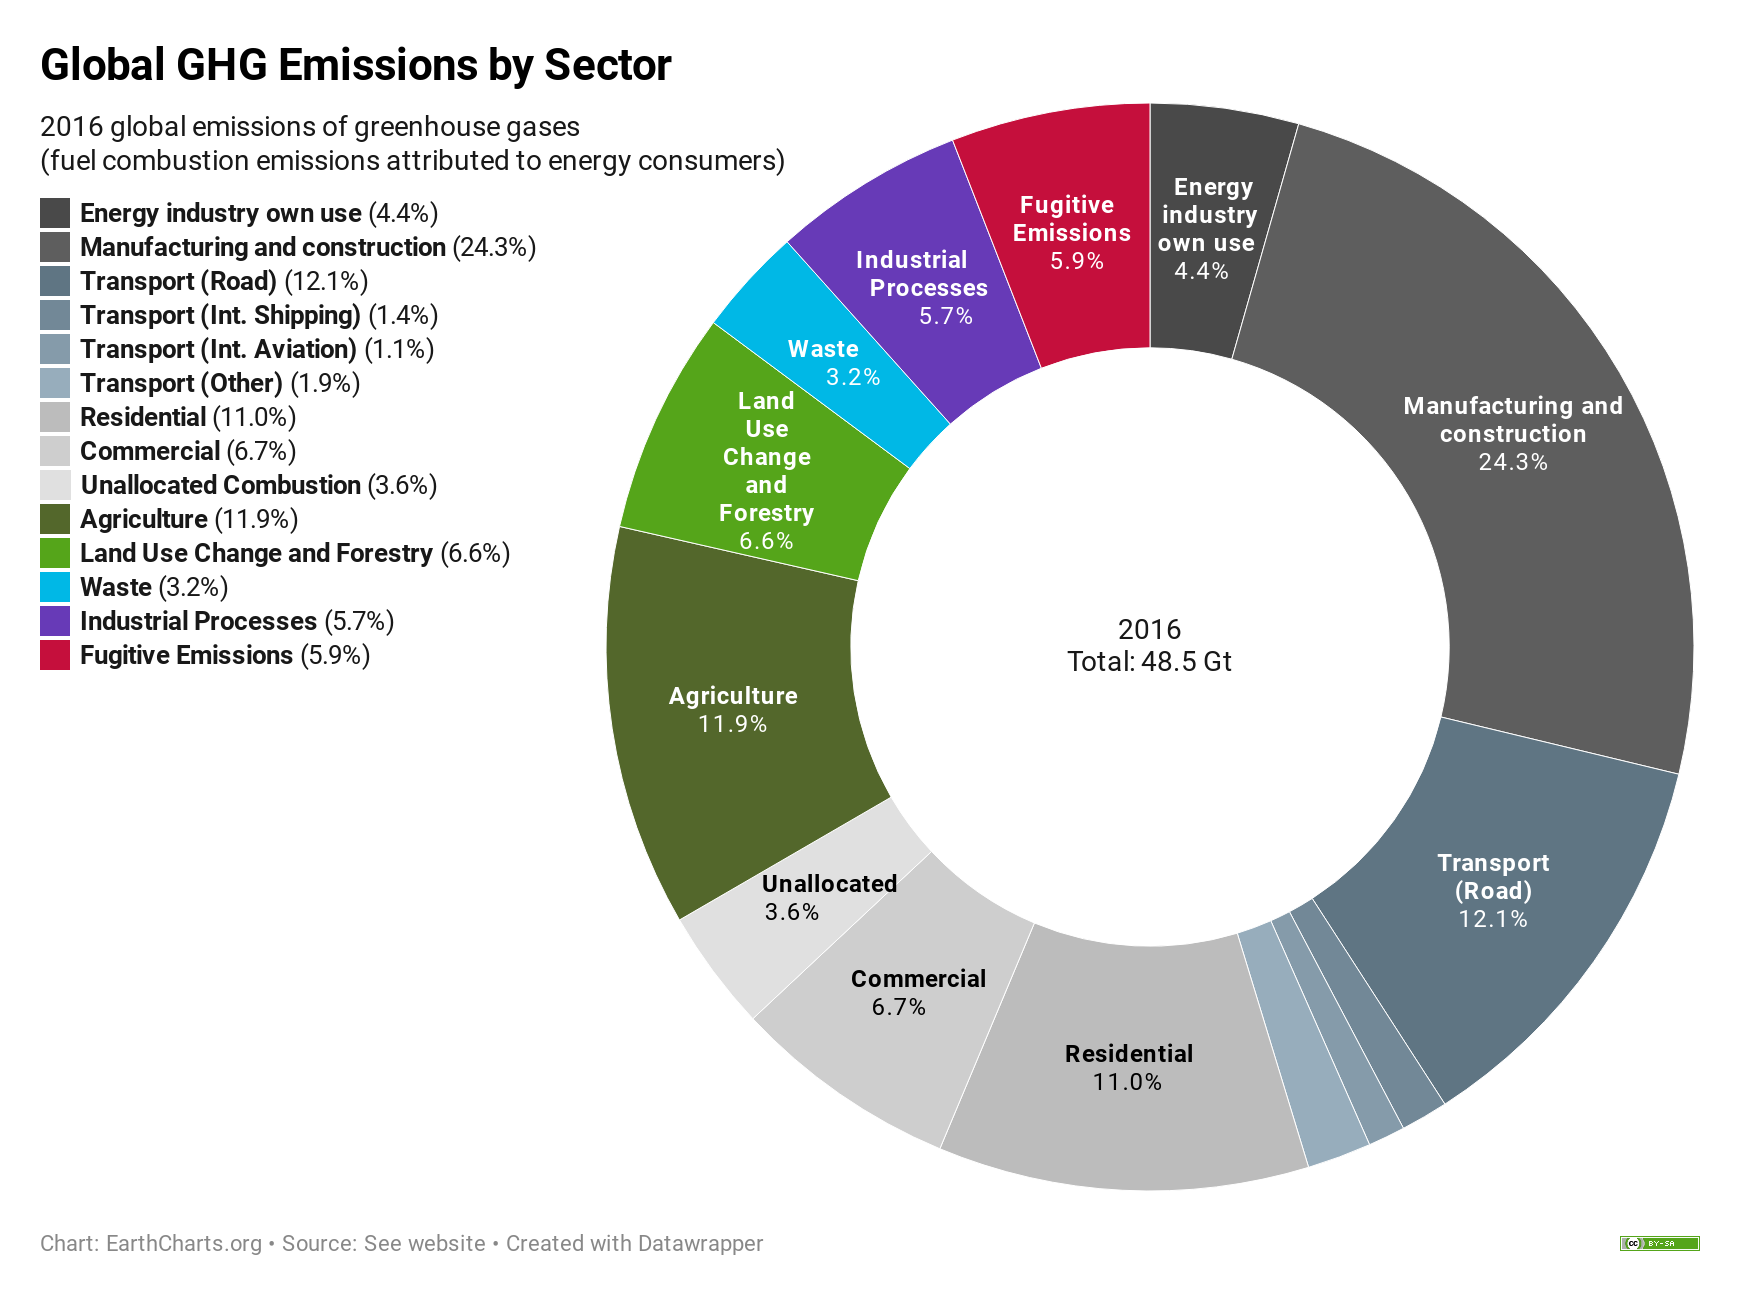
\includegraphics[width=0.95\linewidth]{images/Libro-img026.png}
  \caption{Grafico con le emissioni globali di gas serra del 2016 per settore. 
Credits: By Simon Rayner / EarthCharts - EarthCharts Website (\raggedright\url{http://earthcharts.org/),}
\raggedright\url{http://earthcharts.org/wp-content/uploads/2020/03/Emissions-Sources.png,} CC BY-SA 4.0,
\raggedright\url{https://commons.wikimedia.org/w/index.php?curid=87783234}}
\end{figure}

Quindi è vero che ci sono 100 aziende che sono responsabili del 71\% dell'inquinamento, quindi
anche con lo sforzo della collettività e l'ottimizzazione dei nostri consumi, nella nostra vita
privata, possiamo andare a lavorare solo su una percentuale minore del restante 29\%. O forse no? Le aziende rispondono
in funzione della legge economica della domanda e dell'offerta, Le aziende rispondono anche alla legge economica della domanda e dell'offerta; pertanto, se un numero significativo di industrie e privati cittadini orientasse i propri acquisti verso energia prodotta in maniera pulita, queste aziende sarebbero fortemente incentivate a riconsiderare e accelerare la propria transizione verso una produzione più sostenibile per rimanere competitive. 
Credo comunque sia molto difficile sperare in un cambiamento collettivo e, che i cambiamenti più efficaci sono quelli politici che scoraggino scelte problematiche, ma anche in questo caso dev'esserci una certa pressione da parte dei cittadini che spinga in una certa direzione.
La tendenza, sia nel privato che nelle aziende è tendenzialmente positiva, infatti l'impiego di energie prodotte da fonti
rinnovabili è sempre maggiore di anno in anno, a discapito dei combustibili fossili.

Diversi enti stanno facendo proprio questo, chiamare persone all'azione attraverso eventi,
manifestazioni, petizioni ecc… Potete rimanere informati sugli eventi attraverso i siti o le pagine social, tra i più
importanti possiamo trovare:

greenpeace.org/italy

wwf.it

footprintnetwork.org

fridaysforfutureitalia.it 



E siti di petizioni online:

avaaz.org

wemove.eu

change.org


Potete trovare ulteriori informazioni e grafici su
Wikipedia\endnote{\raggedright\url{https://en.wikipedia.org/wiki/World\_energy\_consumption}}
\endnote{\raggedright\url{https://en.wikipedia.org/wiki/Greenhouse\_gas}}.


\begin{mdframed}[linewidth=1pt]
Uno studio pubblicato su Science Advances\endnote{\raggedright\url{https://www.science.org/doi/epdf/10.1126/sciadv.adh8263}} ha evidenziato che per combattere l’inquinamento indoor non basta semplicemente areare gli ambienti, poiché i composti organici volatili (VOC), che includono sostanze nocive come l’ammoniaca e il benzene, tendono a depositarsi sulle superfici e a rilasciarsi gradualmente nell’aria. La ricerca ha confrontato l’efficacia della ventilazione, sia naturale che con purificatori, con quella della pulizia manuale, scoprendo che attività come passare l’aspirapolvere, spolverare e lavare i pavimenti sono più efficaci nel rimuovere i VOC. Tuttavia, la ventilazione rimane superiore per quanto riguarda l’eliminazione delle polveri sottili, un altro importante fattore dell’inquinamento domestico.
\end{mdframed}

Gli italiani sono spesso abbastanza esterofili e, su tanti aspetti abbiamo anche ragione ad esserlo. Ma ci sono cose, davvero
importanti di cui dobbiamo essere orgogliosi. Abbiamo un ottimo sistema sanitario e in generale il
welfare\endnote{\raggedright\url{https://en.wikipedia.org/wiki/List\_of\_countries\_by\_social\_welfare\_spending}}, ammortizzatori
sociali, malattia, maternità, ferie ecc… Inoltre tra i paesi più industrializzati l'Italia si distingue per un consumo pro capite relativamente basso e sta investendo molte risorse nella conversione verso fonti rinnovabili.

Si potrebbero sollevare diverse critiche sull'Italia, come il fatto che ci sia una forte pressione
fiscale, ma come possiamo vedere nelle mappe qui di seguito, welfare e tasse vanno abbastanza di pari passo anche per gli altri paesi europei. 
Questo non ci deve portare al nazionalismo più cieco, l'Italia ha anche una pressione fiscale alta perché è tra i paesi che evadono di più il fisco, più numerosi altri problemi, come ad esempio l'occupazione.

\needspace{4cm}
\begin{table}[H]
\centering
\caption{Possiamo notare una correlazione tra tasse e welfare. Le mappe sono focalizzate solo sull'Europa in quanto nel resto del mondo non si hanno dati, come potete constatare entrando nella fonte. Inoltre la testa della classifica è composta da stati europei: 1° Francia, 2° Finlandia 3° Belgio 4° Italia, 5° Danimarca, il Giappone si trova in 11° posizione, Nuova Zelanda 21° e Stati Uniti al 23.}
\begin{tabular}{cc}
  \begin{subfigure}{0.5\textwidth}
    \centering
    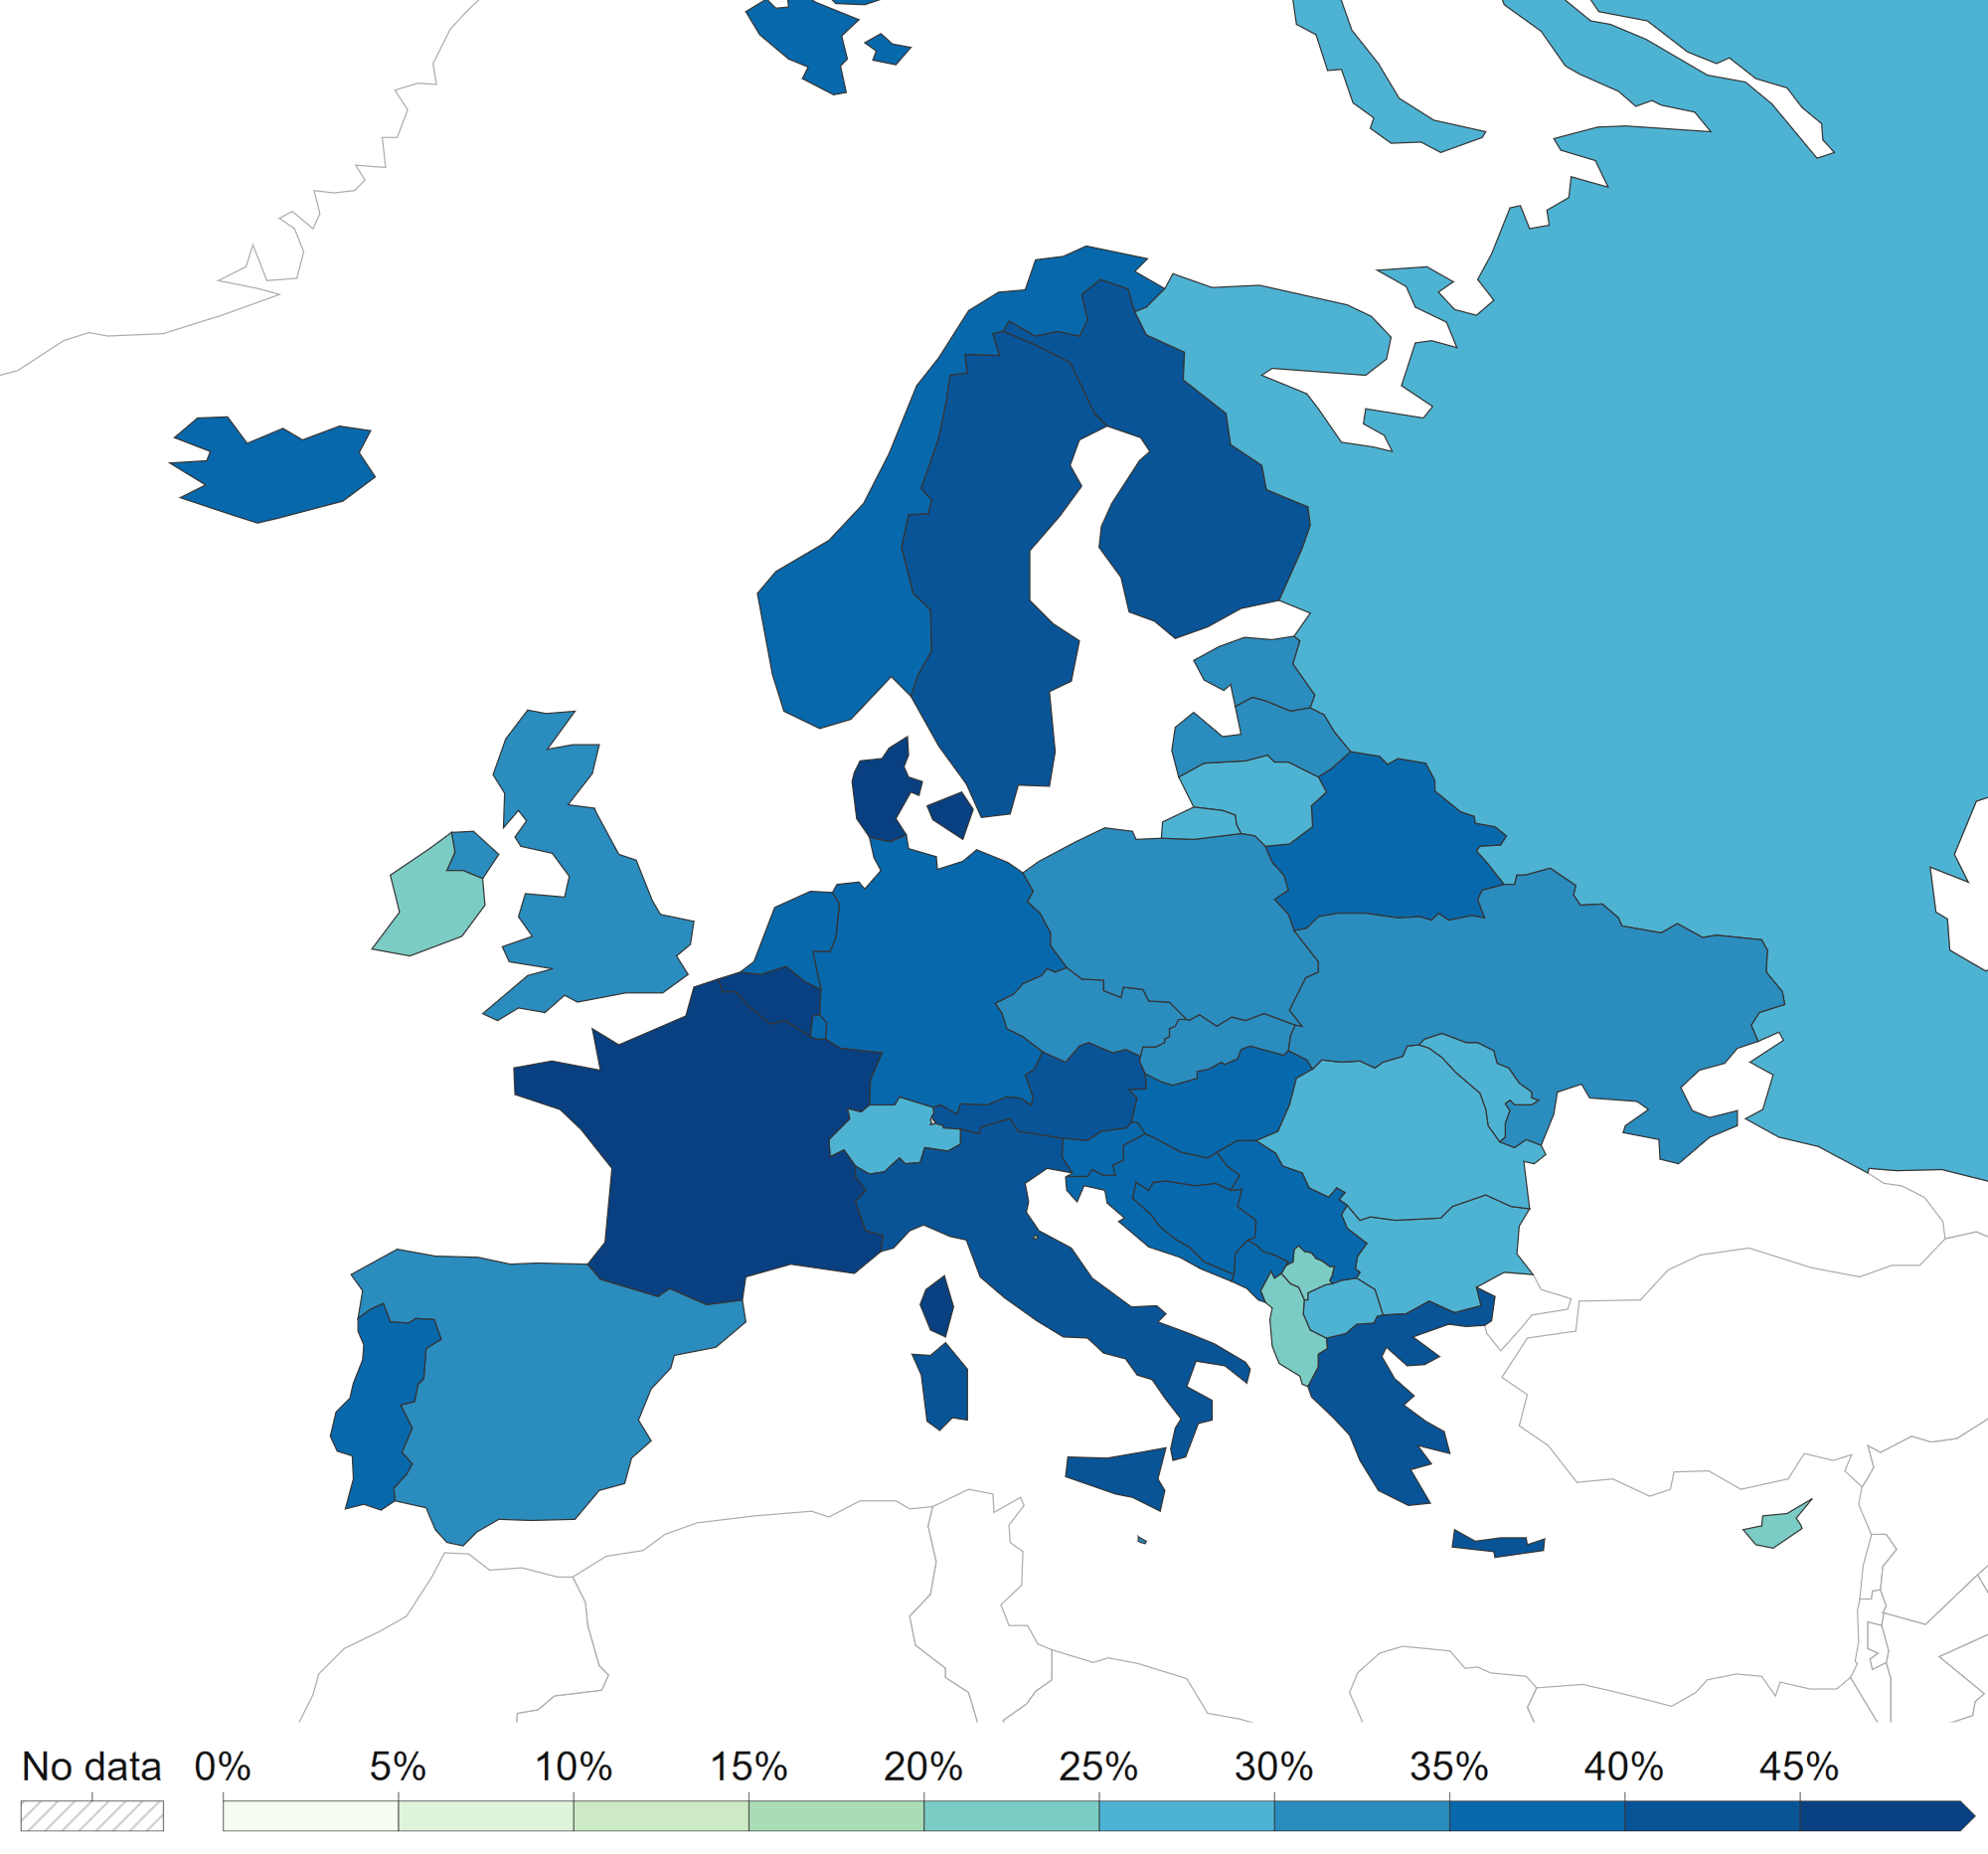
\includegraphics[width=0.8\linewidth]{images/Libro-img028.png}
    \caption{Entrate fiscali totali, 2016 - Fonte: \raggedright\url{https://ourworldindata.org/grapher/total-tax-revenues-gdp?tab=map\&time=2016}}
  \end{subfigure}
  &
  \begin{subfigure}{0.5\textwidth}
    \centering
    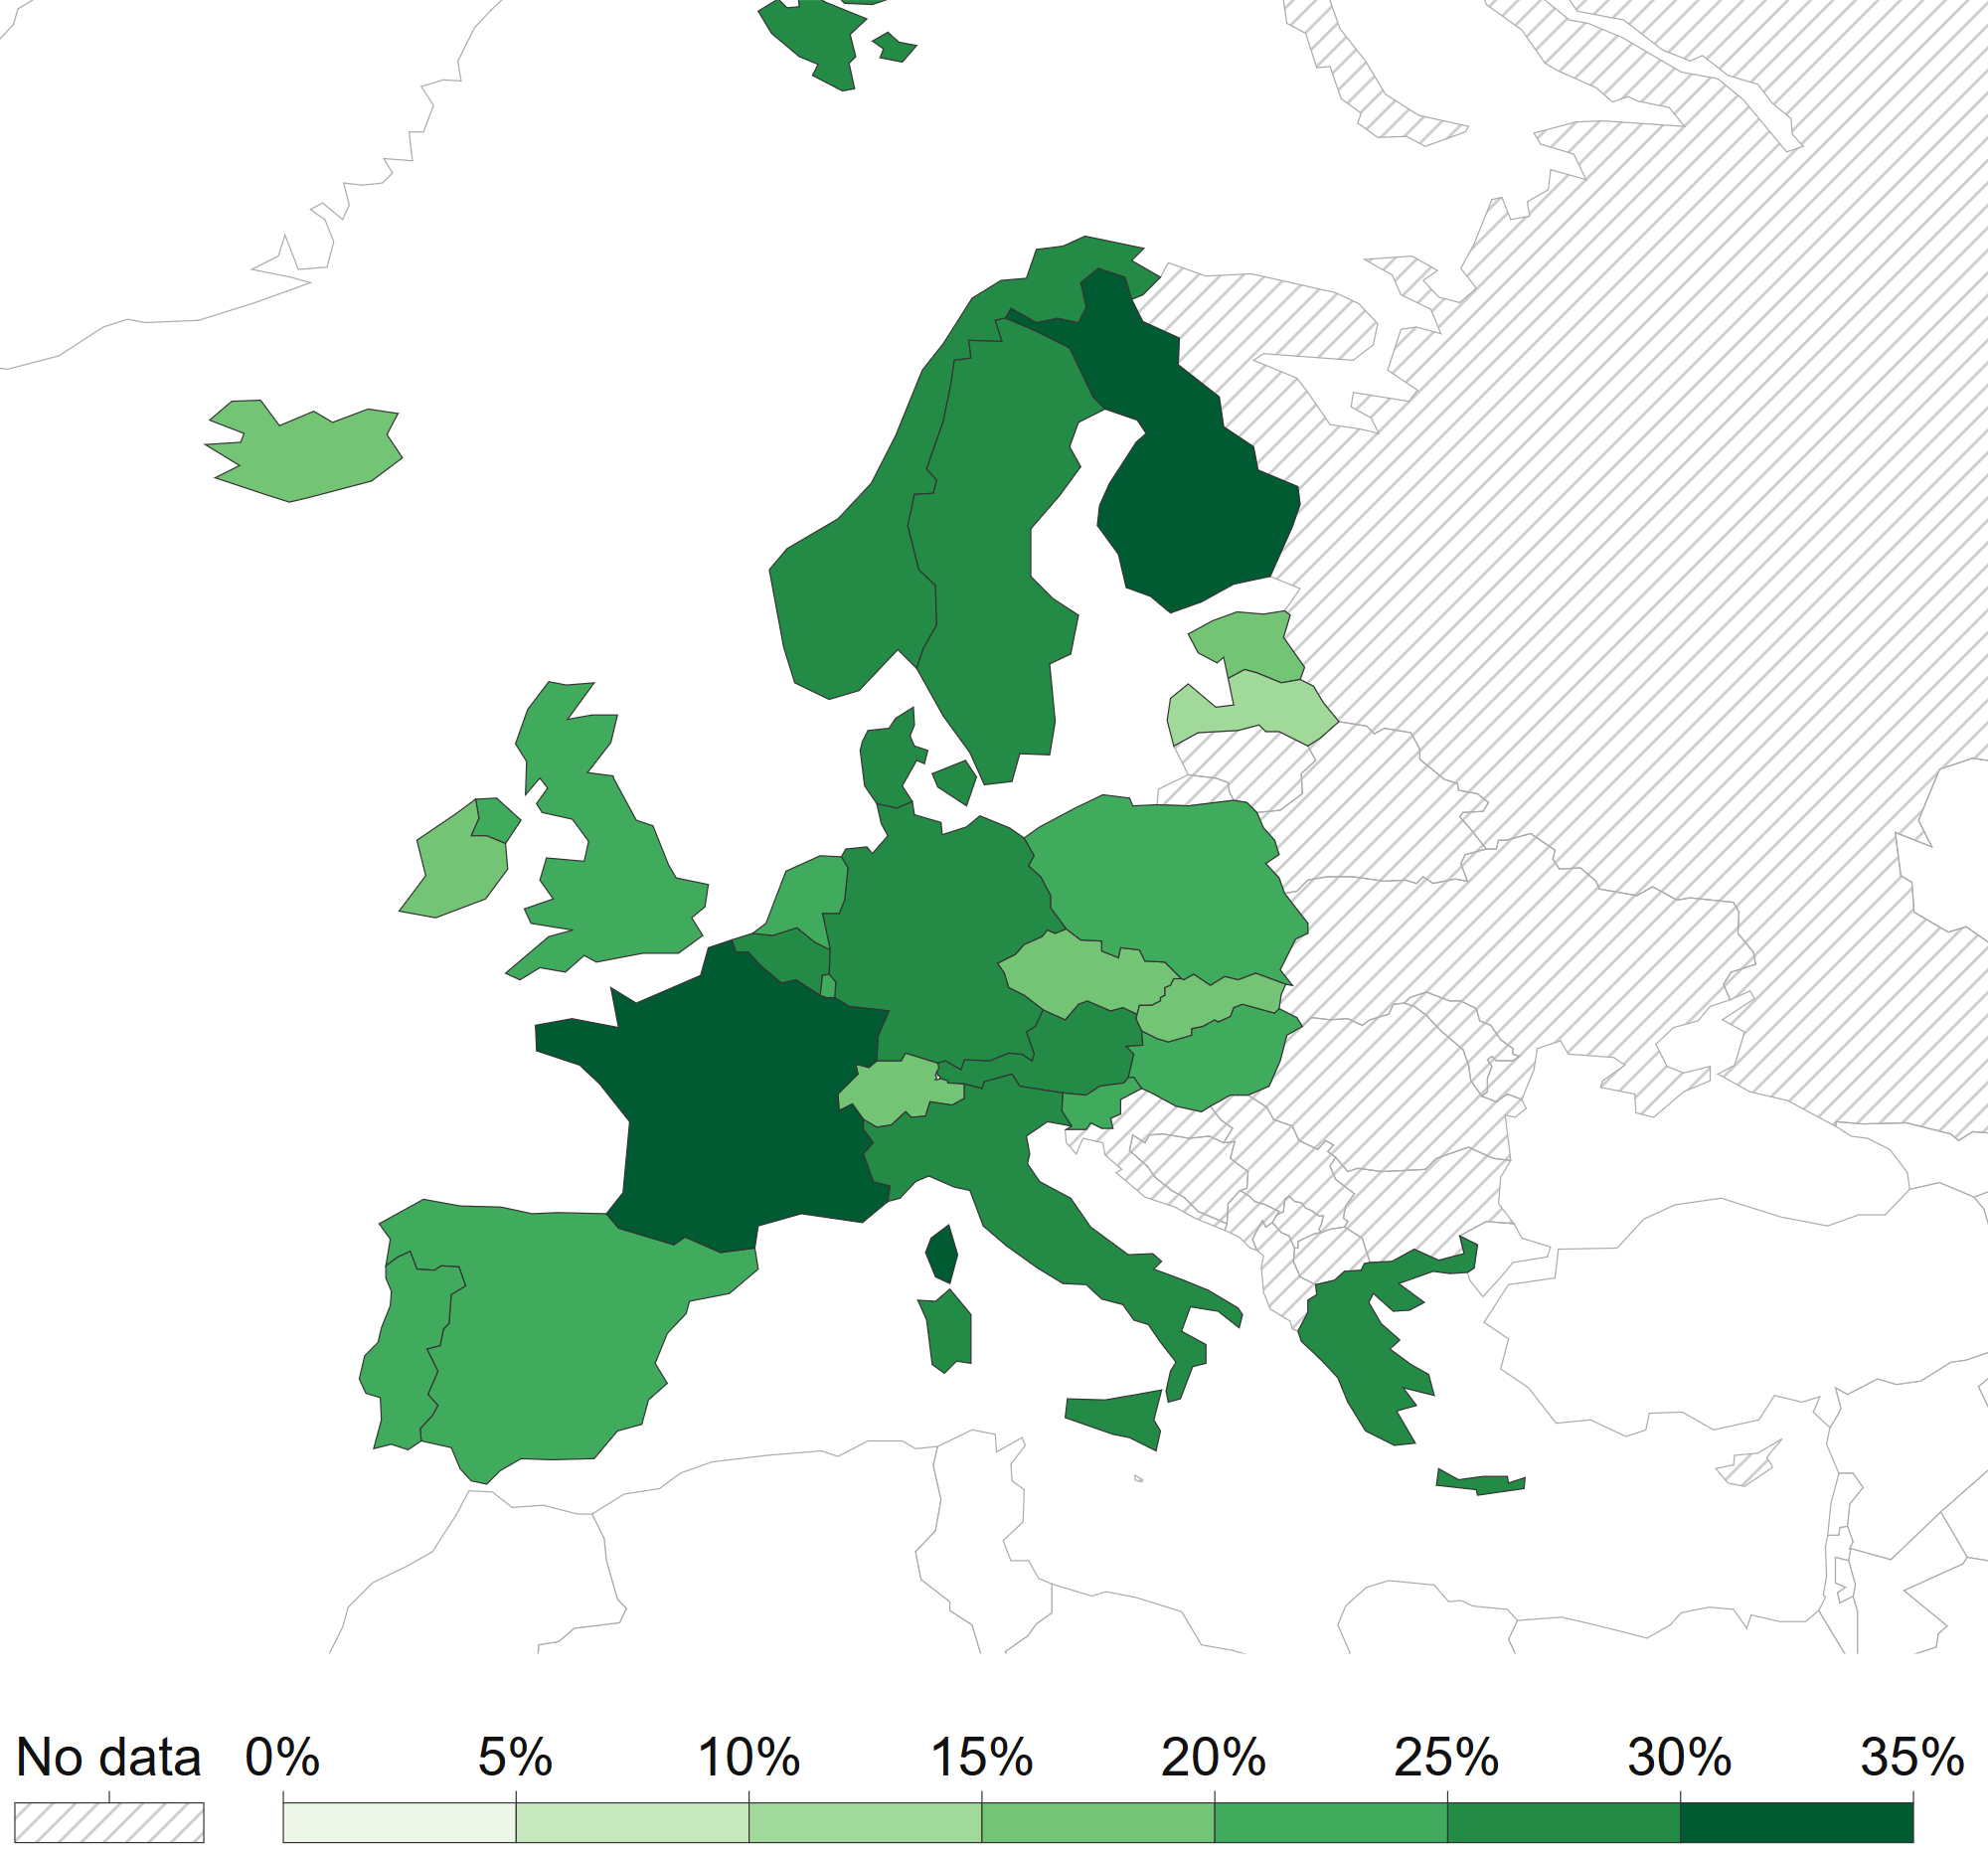
\includegraphics[width=0.8\linewidth]{images/Libro-img029.png}
    \caption{Spesa pubblica sociale in percentuale del PIL, 2016 - Fonte: \raggedright\url{https://ourworldindata.org/grapher/social-spending-oecd-longrun?tab=map}}
  \end{subfigure}
\end{tabular}
\end{table}

Anni fa, scaricando i dati di sugli indici di pace, clima, potere d'acquisto, welfare, sistema sanitario, istruzione, morti per abuso di sostanze, salute mentale e suicidi, ho creato una pagina web\endnote{\raggedright\url{https://iacoposk8.github.io/projects/best-country/}} dove poter assegnare un importanza da 1 a 100 a questi fattori per generare una classifica dei paesi più adatti a noi. Lasciando tutto a 100 l'Italia è in seconda posizione sotto la Danimarca.

\needspace{4cm}
\begin{figure}[H]
  \centering
  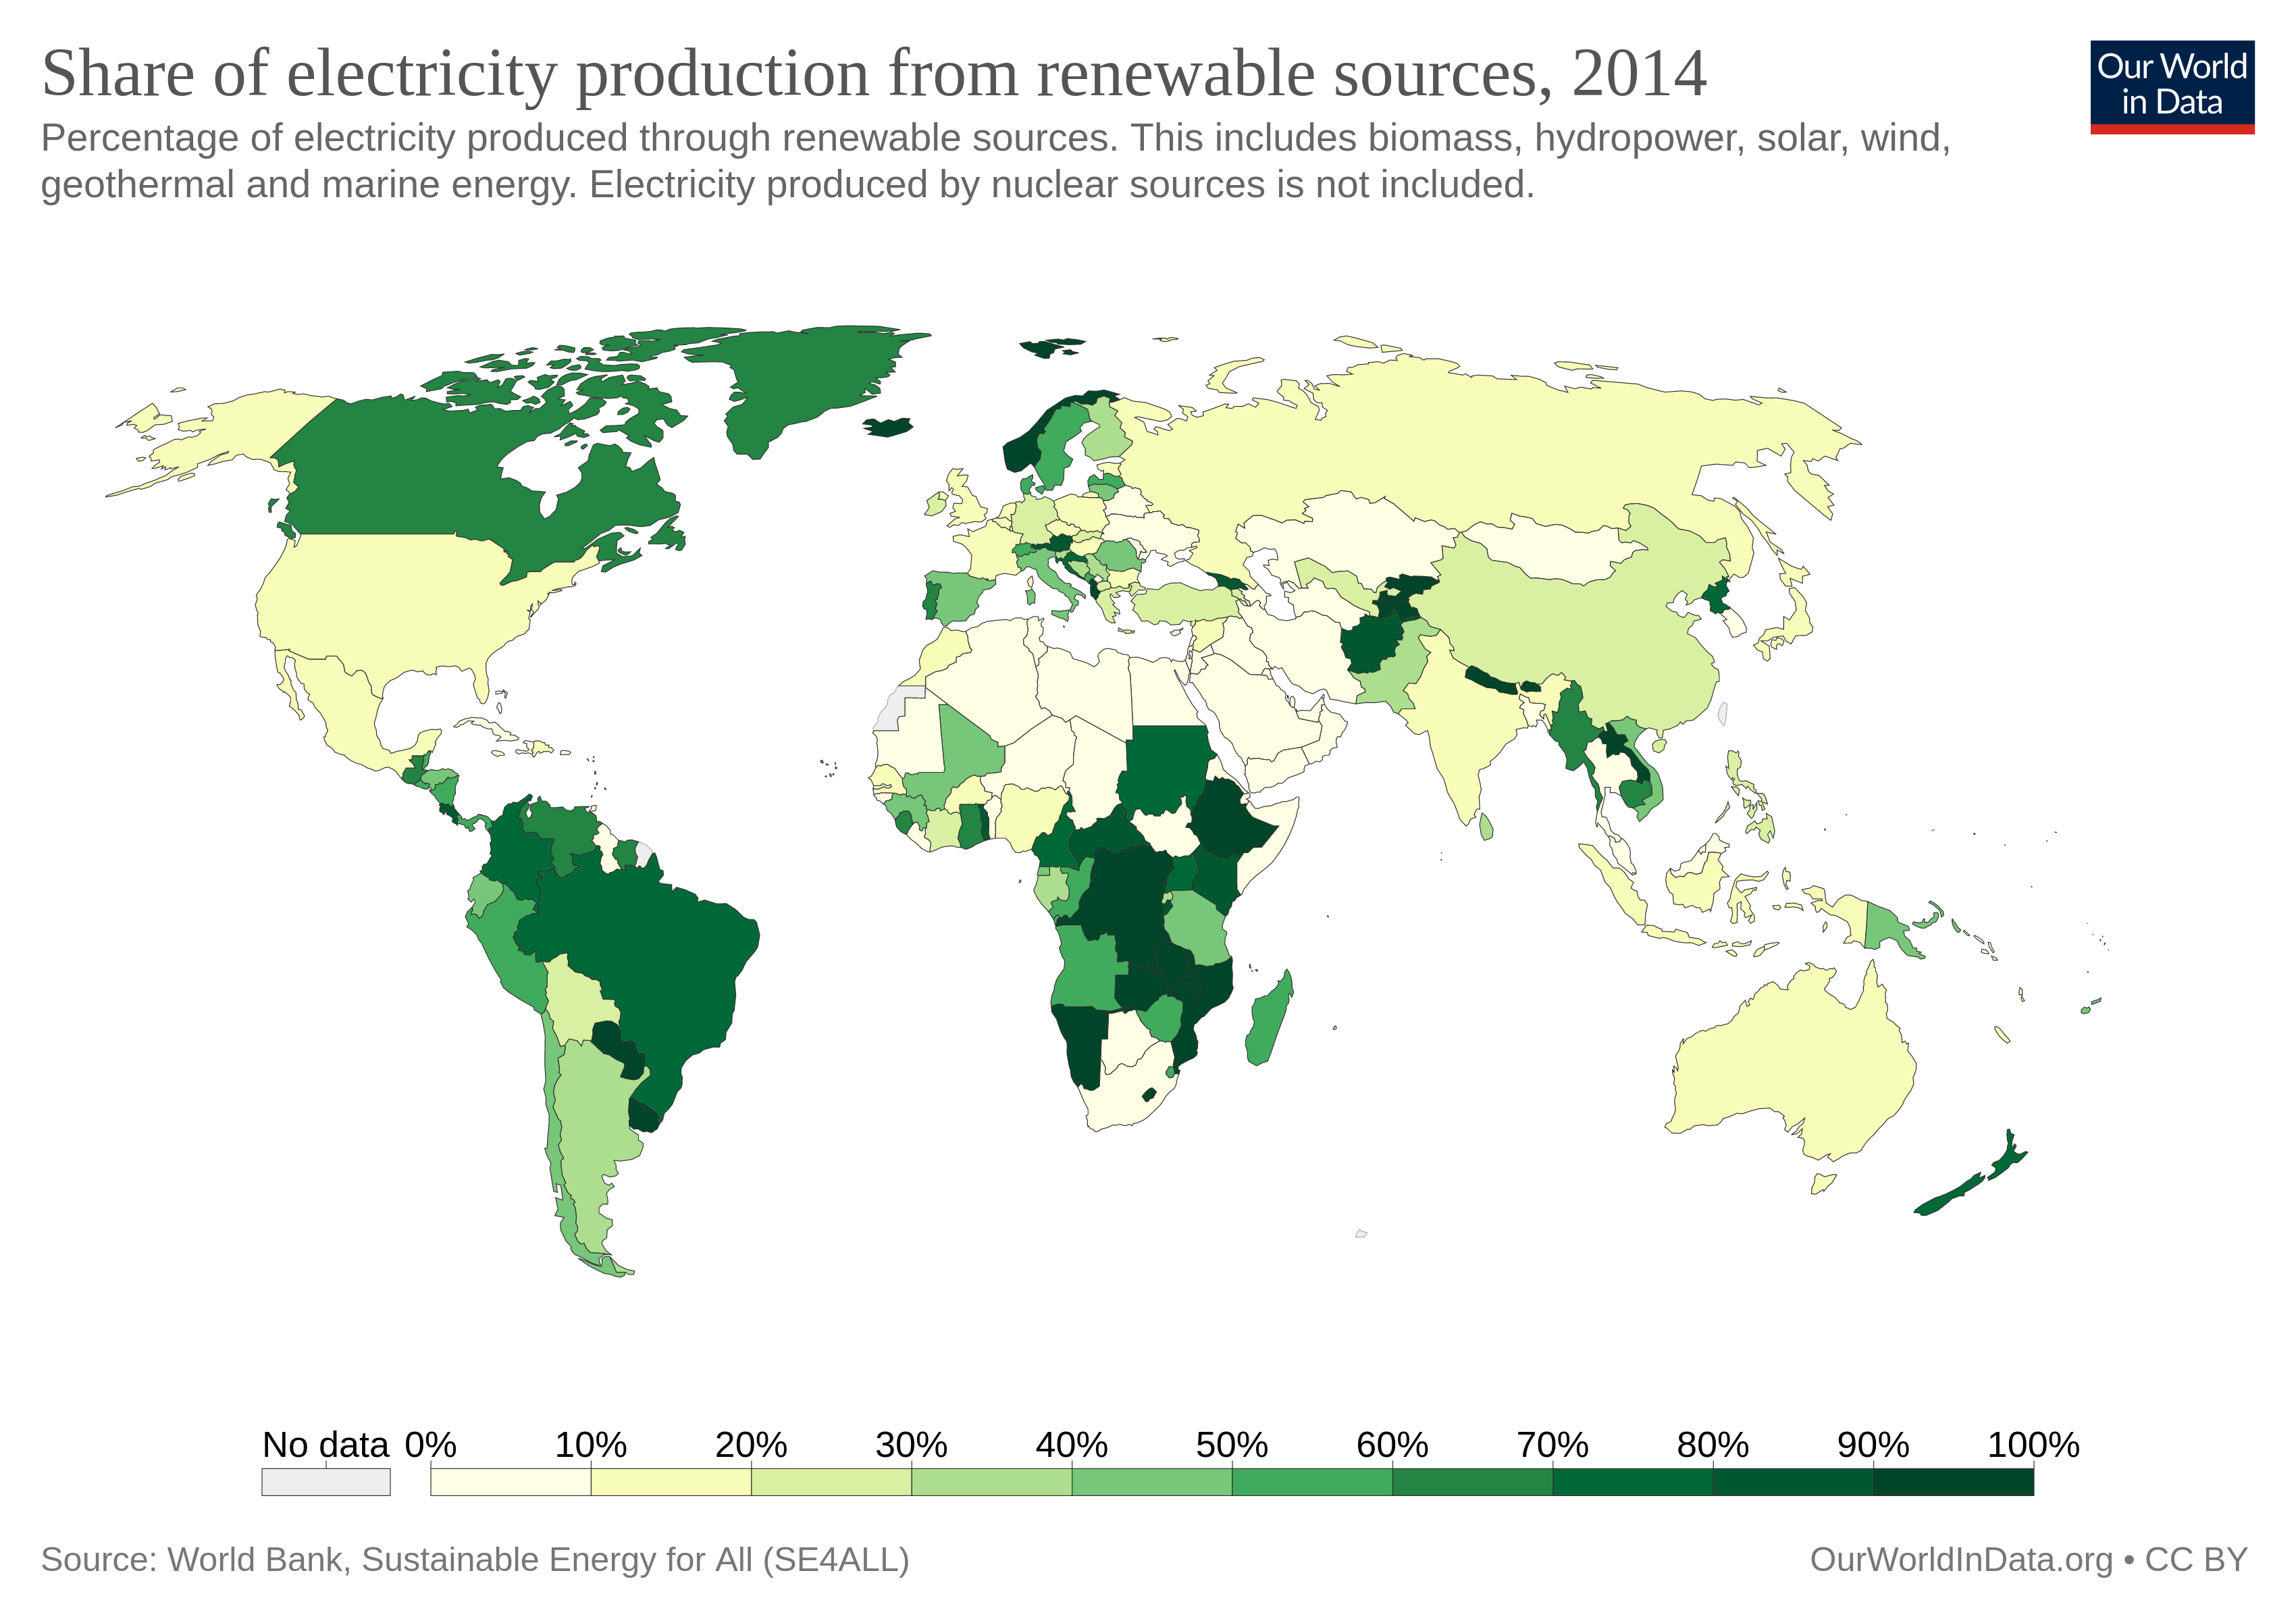
\includegraphics[width=0.95\linewidth]{images/Libro-img027.png}
  \caption{Percentuale di elettricità prodotta attraverso fonti rinnovabili nel 2014. 
Credits: \raggedright\url{https://ourworldindata.org/energy}}
\end{figure}

Le strade percorribili per ridurre la C02 sono tantissime e quotidianamente nascono nuove idee e nuove soluzioni.
Le fonti rinnovabili come l'eolico e il solare, essendo per natura intermittenti e legate alle condizioni meteo, presentano sfide di gestione legate alla loro variabilità nella fornitura di energia. Queste sfide richiedono soluzioni innovative come sistemi di accumulo, gestione intelligente della rete e una diversificazione del mix energetico per garantire l'equilibrio tra domanda e offerta. Un impianto sottostimato non fornirebbe
energia sufficiente a tutti mentre se venisse generata corrente in esubero, a lungo andare provocherebbe problemi
all'impianto elettrico. Tra i vari metodi green, troviamo anche le centrali nucleari. Quando pensiamo alle
centrali nucleari ci viene in mente subito Chernobyl e Fukushima e di conseguenza a radiazioni, morte, disastri, bombe ecc… 
Ma osserviamo il seguente grafico.

\needspace{4cm}
\begin{figure}[H]
  \begin{minipage}{17cm}
    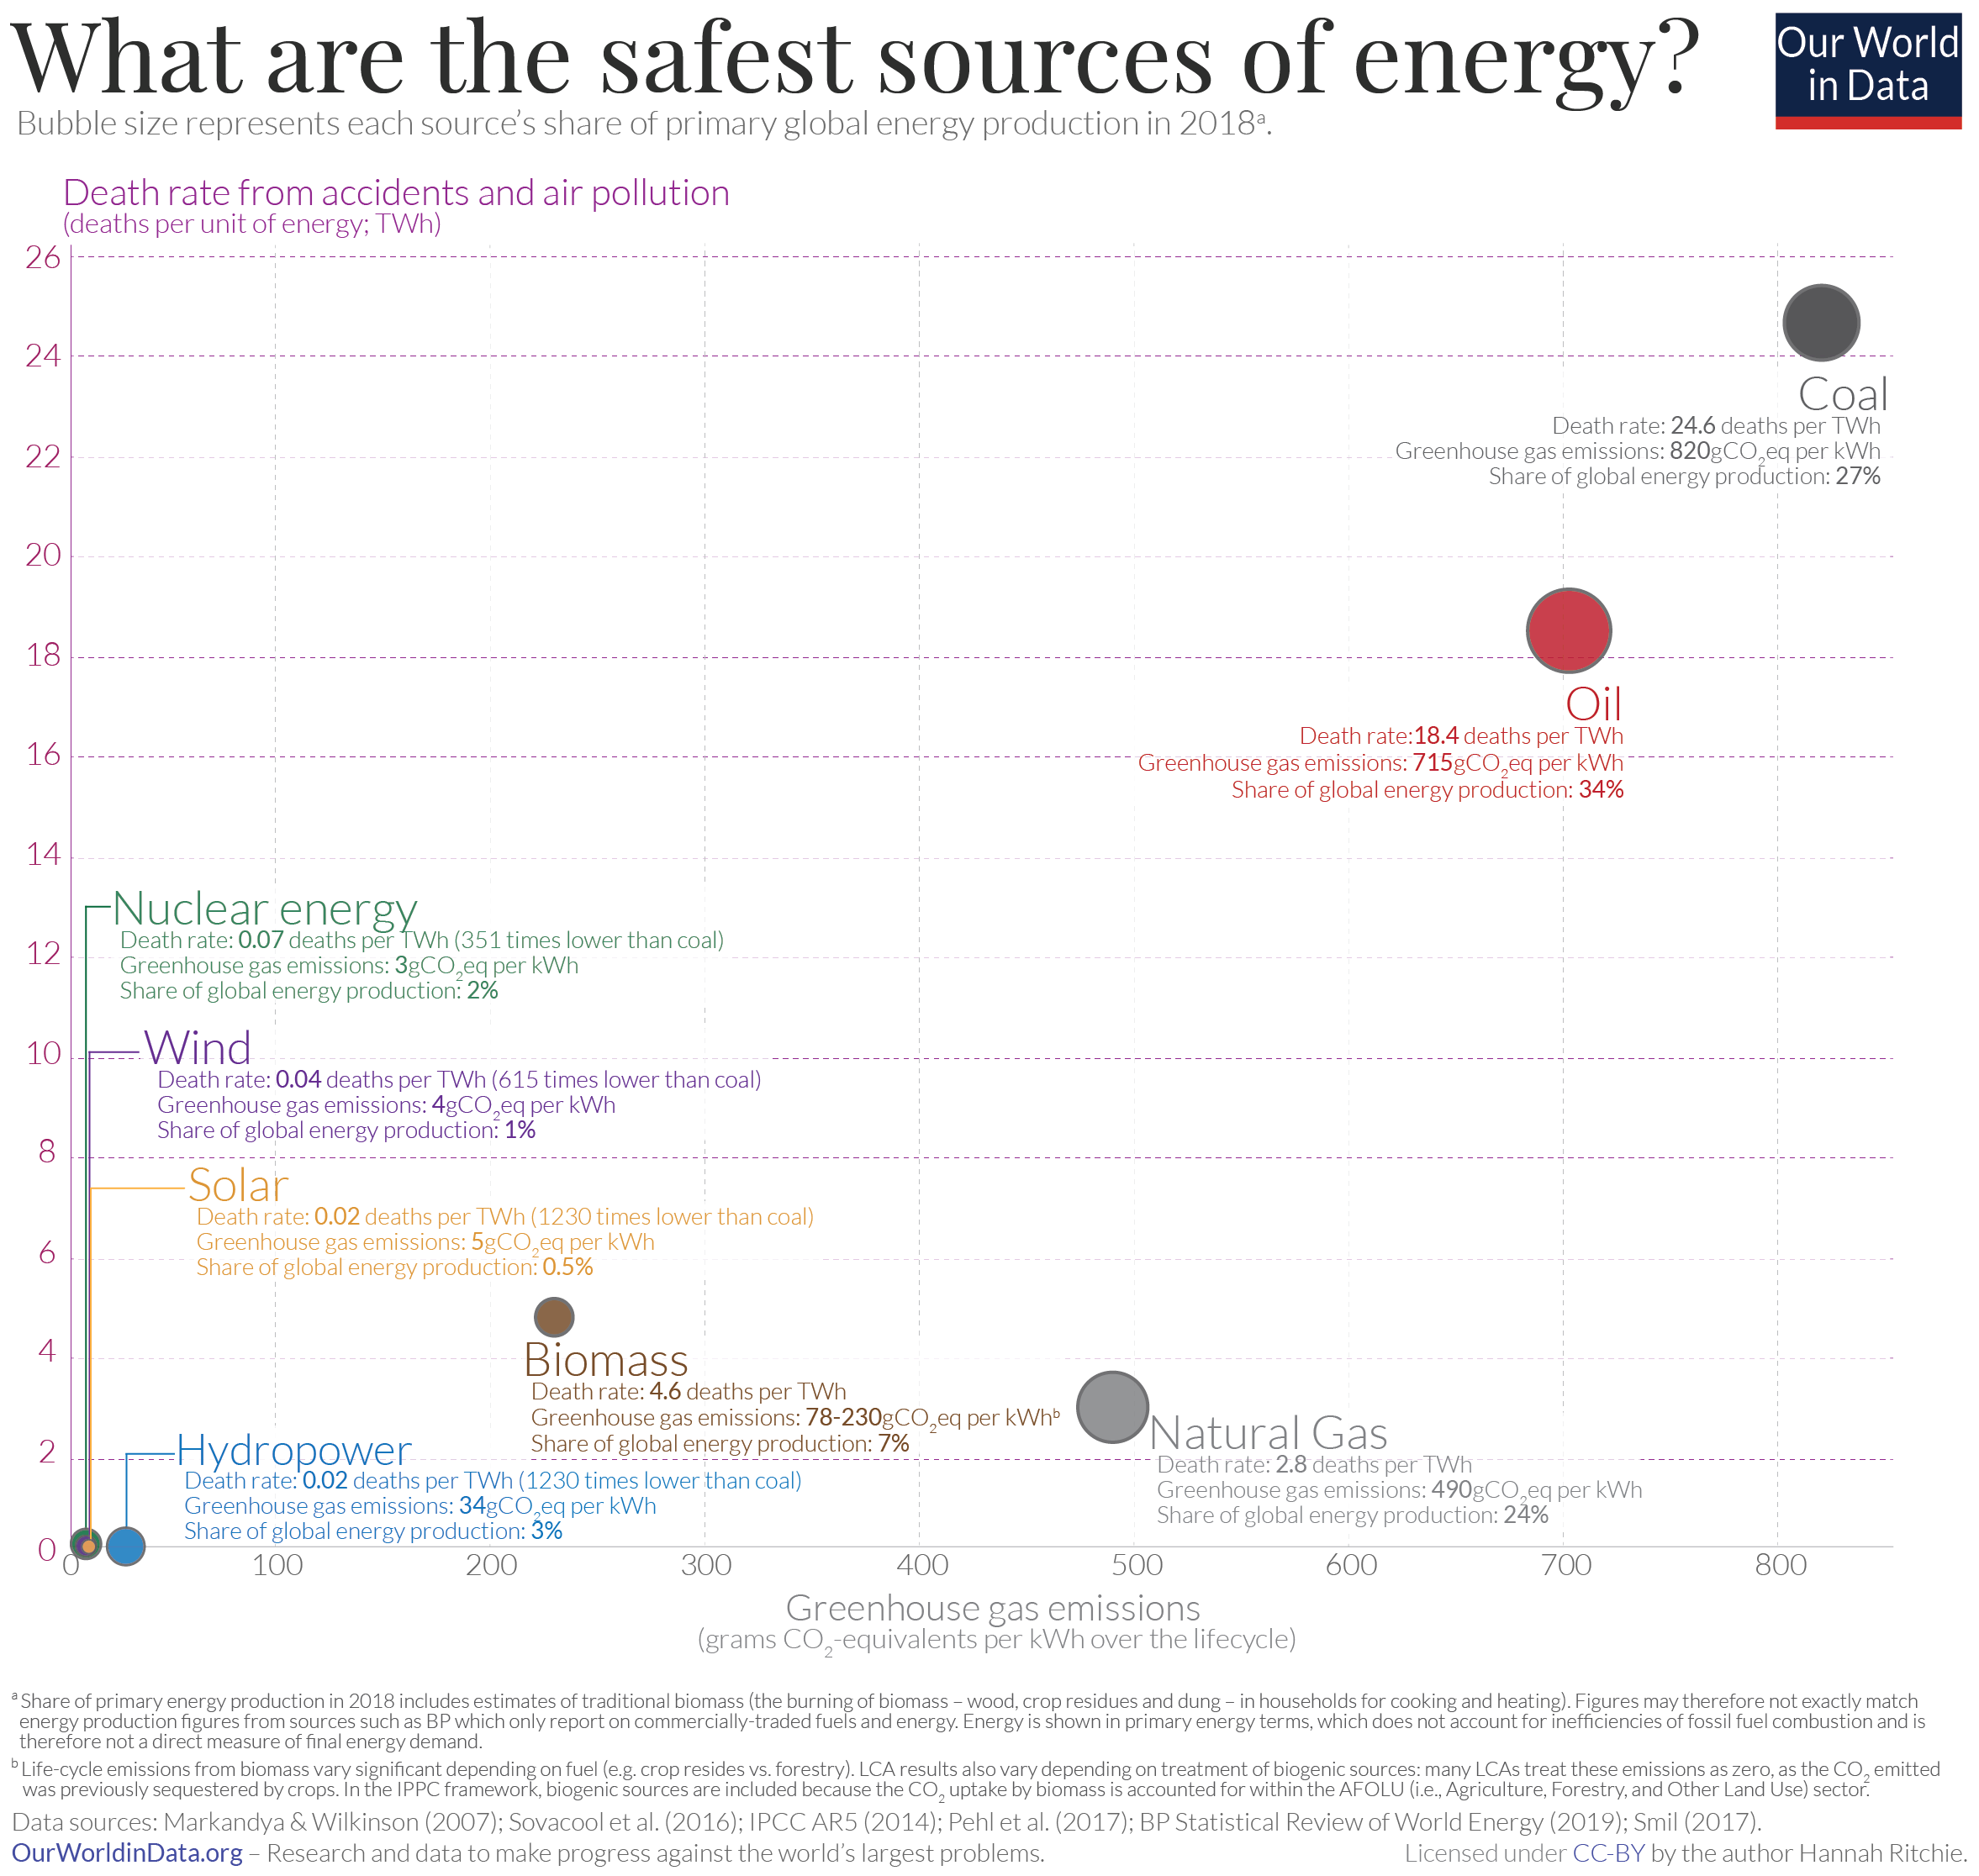
\includegraphics[width=17cm]{images/Libro-img030.png}
    \caption{Credits: \raggedright\url{https://ourworldindata.org/energy} }
  \end{minipage}
\end{figure}

In questo grafico possiamo vedere sull'asse x i gas serra prodotti dalle varie fonti di energia e,
sull'asse y, il numero di morti che ha provocato ogni terawattora. Vediamo come ci sia una
correlazione tra inquinamento e morte. In testa il carbone, seguito da petrolio, gas naturali e biomasse. Possiamo
notare come il nucleare abbia ucciso molte meno persone rispetto al carbone (351 volte meno). Se consideriamo che l'incidente di Chernobyl fu dovuto in gran parte a un reattore con un design intrinsecamente difettoso e a gravi errori operativi, e quello di Fukushima a un evento naturale di portata eccezionale che superò le misure di sicurezza, le moderne centrali nucleari incorporano tecnologie e protocolli di sicurezza avanzati che mirano a ridurre ulteriormente il rischio di incidenti e le potenziali conseguenze. Le centrali nucleari producono scorie radioattive,
ma se isolate correttamente non saranno disperse nell'ambiente. Da queste preoccupazioni nasce il progetto
TerraPower\endnote{\raggedright\url{https://it.wikipedia.org/wiki/TerraPower}} di Bill Gates, che si impegna a risolvere questi due
problemi. L'azienda sta sviluppando una nuova tipologia di reattore chiamata traveling wave reactor (TWR). A differenza dei reattori nucleari tradizionali, che utilizzano uranio arricchito come combustibile e richiedono frequenti interventi umani, il TWR è progettato per funzionare per decenni con minimo intervento umano.
Inoltre, il TWR utilizza uranio impoverito, un sottoprodotto abbondante delle attuali tecnologie nucleari, come combustibile, il che potrebbe permettere di riutilizzare materiali considerati scorie nei reattori convenzionali. Inoltre, come ha spiegato Solomon Goldstein-Rose in un
Ted\endnote{\raggedright\url{https://www.ted.com/talks/solomon_goldstein_rose_how_much_clean_electricity_do_we_really_need}} non basterà convertire la produzione attuale di corrente da combustibile fossile a fonti rinnovabili, servirà
produrne 12 volte tanto. Questo perché molti strumenti stanno diventando elettrici, nella mobilità e non sono, inoltre
i paesi in via di sviluppo cresceranno, aumentando di conseguenza il loro fabbisogno energetico. In più avremo bisogno
di nuove tecnologie, come quelle impiegate nella rimozione del carbonio prodotto negli anni e, anche questo necessiterà
di energie. Per questi motivi, secondo diversi esperti, il nucleare sarà indispensabile e forse non sufficiente.

Al contempo, altri ricerche sono contrarie a queste tecnologie in quanto, nel caso dell'Italia, già
ad oggi, come visto nel precedente grafico, produce già il 40\% di elettricità da fonti
rinnovabili\endnote{\raggedright\url{https://ourworldindata.org/grapher/share-electricity-renewables}}
\endnote{\raggedright\url{https://www.terna.it/it/sistema-elettrico/statistiche/pubblicazioni-statistiche} } e, secondo Enel e The
European House, il nostro paese potrà raggiungere la quasi completa decarbonizzazione entro il 2050 e senza bisogno di
energia
nucleare\endnote{\raggedright\url{https://www.ambrosetti.eu/news/net-zero-e-conomy-2050-roadmap-di-decarbonizzazione-per-leuropa/}}.
La costruzione di centrali nucleari inoltre richiede molto tempo e denaro, ma sostenitori invece\endnote{\raggedright\url{https://www.ted.com/talks/isabelle_boemeke_nuclear_power_is_our_best_hope_to_ditch_fossil_fuels}} portano altri esempi, di come la Francia sia riuscita a costruire 45 reattori in 15 anni. O più di recente, Giappone, Cina e Corea hanno costruito reattori in 6 anni circa.

\begin{mdframed}[linewidth=1pt]
Attenzione alla lavatrice

Diverse delle micro plastiche presenti negli oceani arrivano dalle lavatrici. Lavaggi troppo caldi oltre a rovinare
gli indumenti possono separare delle micro fibre dai nostri capi che verranno poi rilasciati
nell'acqua. Una delle migliori scelte ecologiche è proprio impostare un ciclo di lavaggio breve e
con temperature non superiori a 20 °C, utilizzando un additivo igienizzante se vogliamo sentirci più protetti dai
batteri. Oltre all'ambiente questa scelta preserverà più a lungo forma e colore dei vostri capi,
riducendo il rilascio di microfibre sintetiche nell'ambiente fino al 52\% oltre a un consumo inferiore di acqua ed
elettricità. Questo è quello a cui sono arrivati i ricercatori dell'Università di Leeds
(UK)\endnote{\raggedright\url{https://www.sciencedirect.com/science/article/abs/pii/S0143720819320431}}.
\end{mdframed}

\subsection{Sicurezza}
Premetto dicendo che l'utilizzare la storia come filtro per interpretare il presente, secondo me, può essere fuorviante, poiché richiede una notevole capacità di astrazione. Ad esempio, confrontare il riarmo che precedette la Prima Guerra Mondiale con il riarmo attuale è problematico: all’epoca, gli Stati europei si osservavano con sospetto reciproco, e ogni incremento militare generava timore nei vicini. Inoltre, non esisteva ancora la deterrenza nucleare. Per questo, anche se le dinamiche possono sembrare simili, il contesto storico è così diverso da rendere difficile una lettura delle due situazioni. 

Può succedere che le persone, come singoli individui o come gruppo di una società, nel cercare
di risolvere un problema, causato da una catena di avvenimenti, guardino solo l'ultimo anello
tentando di risolvere solo quello. Se noi eliminiamo solo lo strato più superficiale senza intervenire sulla
causa che sta alla base, il problema potrebbe ritornare in futuro.

Perché ci sono persone che minano il tessuto sociale rendendo difficile la convivenza, commettendo atti criminali?
Come possiamo evitare che ciò accada a più livelli? Da chi ruba a chi si fa esplodere per un credo?
Chi di noi si farebbe esplodere per denaro o qualsiasi altro motivo? Credo nessuno.
Le motivazioni dietro gesti così estremi sono complesse e multifattoriali. In alcuni casi, condizioni di estrema povertà possono spingere individui a compiere atti disperati, anche per sostenere la propria famiglia.
Allo stesso modo ci si può trovare a rubare quando non abbiamo una rete di supporto e stiamo attraversando un lungo periodo di indigenza.
Non sempre chiaramente, alcuni potrebbero commettere questi atti per fanatismo o avidità.
La povertà o più in generale la necessità possono favorire la criminalità, ma non sono la sola causa, esistono infatti paesi con un PIL basso ma con altrettanto bassi livelli di criminalità come il Bhutan ad esempio.

Tutto questo per dire che non basta semplicemente mettere più disincentivi per scoraggiare la criminalità, seppur sembri sufficiente, ma bisognerebbe capire l'origine del problema, crimine per crimine e capire come intervenire alla radice.

Il carcere ad esempio si è spesso osservato essere una misura inefficace, infatti circa il 70\% dei detenuti, una volta scontata la pena, dopo un breve periodo di libertà, finirà nuovamente in detenzione. Non esiste infatti una correlazione tra numero di carceri o detenuti e sicurezza del paese. Il carcere quindi non è la misura migliore per rieducare le persone, ma è necessaria nel caso in cui un individuo possa essere pericoloso per gli altri.
I Reati violenti si attestano sotto il 10\% in numerose stime, quindi per la maggioranza dei detenuti è possibile pensare a misure che possano davvero rieducarli.
Qualcuno potrebbe dire: perché andrebbero aiutati? Anche egoisticamente la detenzione è un costo, quindi se riuscissimo a trasformare delle persone da spesa a contribuenti sarebbe l'ideale. Ogni anno le carceri costano tre miliardi di cui il 70\% va al personale interno e il 2\% a realtà esterne,
assistenti sociali ecc…
Nel libro "Abolire il carcere. Una ragionevole proposta per la sicurezza dei cittadini" \endnote{\raggedright\url{https://www.amazon.it/dp/8832964961}} si valutano alcune alternative come affidamento, servizi sociali e domiciliari, che hanno portato il tasso
di recidività dal 70\% al 20\%. Anche chi esce con l'indulto ha meno probabilità di entrare nuovamente in carcere. 
Uno dei motivi per cui il carcere ha un alta recidività, dipende anche dal non intervento delle cause che hanno portato quella persona a delinquere.
Se una persona ruba perché non ha soldi, una volta uscita dal carcere si ritroverà nella stessa situazione.
Se volesse cambiare vita potrebbe cercare un lavoro, ma negli anni di detenzione non avrà potuto ampliare il suo curriculum di esperienze lavorative e talvolta anche di istruzione. Inoltre, avere un buco nel curriculum è penalizzante nel trovare una occupazione. 
Se siamo senza una rete di supporto, più il tempo di disoccupazione aumenta, più le probabilità di ritornare a delinquere aumentano.
In carcere succede che le persone, oltre alla libertà, vengono privati anche di affetti e intimità, in quanto andare
a trovare un carcerato è piuttosto complicato, anche i parenti, iniziano a fare visita sempre meno. 
Un individuo che ha vissuto in un ambiente ostile, tra guardie e detenuti, spesso esce dal carcere con un atteggiamento ancora più incattivito nei confronti del Sistema. Non solo cercherà di non farsi beccare la prossima volta, ma durante la detenzione potrebbe aver stretto legami con altre persone che gli hanno insegnato nuovi modi per delinquere.
Ma possiamo fare un’altra scelta: possiamo trasformare la popolazione carceraria da costo a risorsa, impiegandola in lavori socialmente utili o in aziende agricole e artigiane, che spesso hanno bisogno di manodopera stagionale. In questo modo i detenuti vengono realmente reinseriti nella società, non isolati, imparano un mestiere e conoscono persone in grado di offrire una nuova possibilità.
È anche così che si protegge la collettività: riducendo la recidiva e creando ponti tra il dentro e il fuori. Lo stress che le forze dell’ordine affrontano ogni giorno ci consente a noi di vivere serenamente, e per questo meritano rispetto. Ma il loro lavoro sarà ancora più efficace se sarà parte di un sistema che non si limita a punire, ma che educa, responsabilizza e reintegra.

La pena dovrebbe essere commisurata al reato. Una persona
che commette un reato economico generalmente dovrà essere punita economicamente, non con la libertà.
Dico generalmente perché abbiamo casi in cui un truffatore rovina migliaia di famiglie o evasori fiscali seriali che sottraggono miliardi allo stato. Molti in questi casi sosterrebbero che il danno sociale è così vasto da meritare una pena detentiva.

Se si depenalizzassero le droghe leggere, la popolazione carceraria andrebbe a calare in quanto molti dei detenuti
hanno una condanna per spaccio. Questo porterebbe ad avere meno processi e quindi una giurisdizione più veloce ed efficiente,
ma anche più soldi da impegnare in attività di recupero del carcerato. Il Portogallo ad esempio ha depenalizzato il
consumo di tutte le droghe nel 2001, sia leggere che non e, con ottimi risultati: Secondo un rapporto del 2017
dell'Institute of Labor
Economics\endnote{\raggedright\url{https://www.iza.org/publications/dp/10895/going-after-the-addiction-not-the-addicted-the-impact-of-drug-decriminalization-in-portugal}}, la depenalizzazione “ha contribuito a un calo nel numero di sequestri di eroina e cocaina, una diminuzione del
numero di reati e decessi per droga e una diminuzione del numero di pazienti che entrano in cura”. 

Oltre ad intervenire sul lavoro è importante lavorare sull'istruzione, in quanto correlata alla delinquenza\endnote{\raggedright\url{https://italiaindati.com/carceri-in-italia/}}.

\begin{mdframed}[linewidth=1pt]
Avere un'arma in casa ci rende più sicuri?

Secondo numerosi studi, la risposta è negativa. Un'analisi di 15 studi ha rilevato che tenere un'arma da fuoco in casa quasi raddoppia la probabilità di essere assassinati. Uno studio della Emory University\endnote{\raggedright\url{https://journals.lww.com/jtrauma/Abstract/1998/08000/Injuries\_and\_Deaths\_Due\_to\_Firearms\_in\_the\_Home.10.aspx}}, condotto su 626 casi avvenuti in casa in tre città statunitensi (Memphis, Seattle e Galveston), ha osservato che gli spari accidentali sono quattro volte più frequenti di quelli per autodifesa, mentre quelli per compiere un'aggressione o un omicidio sono sette volte superiori, e undici volte più frequenti sono i colpi per suicidio. Secondo il Injury Control Research Center di Harvard, le armi sono usate per autodifesa in meno dell'1\% delle aggressioni con una vittima. John Donohue, economista della Stanford University, ha osservato nel 2017 che la riduzione dei requisiti per il porto d'armi in uno Stato porta a un aumento dei crimini violenti.

In Italia, non esiste un rapporto ufficiale del Viminale sugli omicidi con armi da fuoco legalmente detenute, una mancanza significativa. Un’indagine svolta da Fire-Transcrime in collaborazione con l'Università Cattolica di Milano ha osservato che, nei paesi europei, gli omicidi con armi da fuoco tra il 2010 e il 2015 hanno causato vittime principalmente in ambito familiare (34\%) e interpersonale (32\%), mentre solo il 21\% è attribuibile a gruppi criminali organizzati, il 10\% ad atti criminali e il 3\% a motivi socio-politici. Questo suggerisce che in Europa, e presumibilmente anche in Italia, la maggior parte degli omicidi con armi da fuoco avviene in contesti familiari o interpersonali (66\%)\endnote{\raggedright\url{https://www.rivistailmulino.it/a/legittima-difesa-una-modifica-ingannevole-e-pericolosa}}.

Prima di ipotizzare una legalizzazione più estesa della legittima difesa armata, sarebbe opportuno introdurre incentivi per l'installazione di sistemi di sicurezza passivi, come antifurti, videosorveglianza o dispositivi dissuasivi non letali. Questi strumenti, oltre a essere più sicuri, contribuiscono a prevenire i reati senza introdurre nuovi rischi all'interno delle abitazioni.

In sintesi, gli studi suggeriscono che la presenza di armi in casa non aumenta la sicurezza personale, ma accresce il rischio di incidenti. Questi incidenti stanno portando a soluzioni creative come la PaintCam\endnote{\raggedright\url{https://www.kickstarter.com/projects/paintcam/paintcam-face-recognition-and-paintball-firing-security-system}} una videocamera di sorveglianza che spara vernice e lacrimogeni agli intrusi.
\end{mdframed}

\needspace{8cm}
\begin{mdframed}[linewidth=1pt]
Droga
\begin{wrapfigure}{i}{4.972cm}
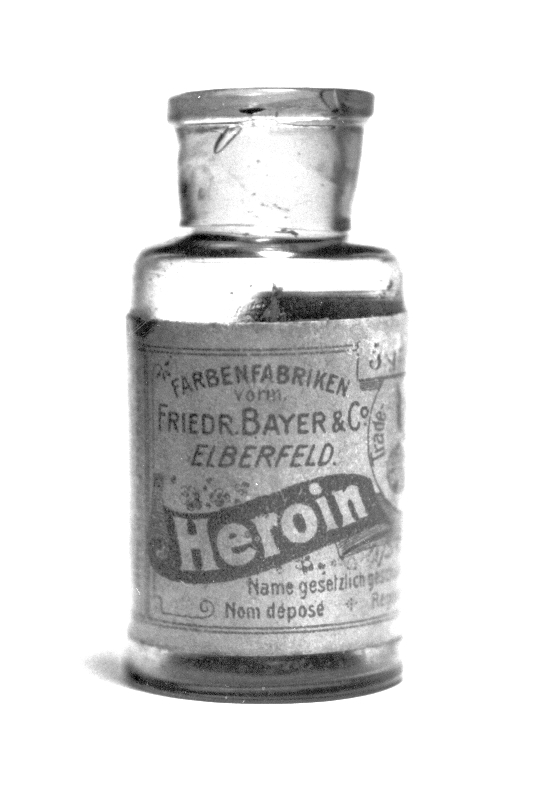
\includegraphics[width=4.972cm,height=7.287cm]{images/Libro-img054.jpg}
\caption*{Di Mpv\_51 at English Wikipedia - Transferred from English Wikipedia, Pubblico dominio, \raggedright\url{https://commons.wikimedia.org/w/index.php?curid=546164} }
\end{wrapfigure}

Ginevra, in Svizzera, a fine degli anni 80 si è trovata ad affrontare una crisi sanitaria legata al consumo di eroina e dell'HIV. Le due
strade percorribili al fine di risolvere questo problema, principalmente sono due, liberalizzazione o repressione. Ginevra ha scelto la
prima strada, in una maniera più attiva di altri esempi che abbiamo sparsi per il mondo. Hanno compreso che l’eliminazione totale della droga non è realistico, e si sono focalizzati su misure pragmatiche di riduzione del danno. 
Il loro obiettivo non è rimuovere la droga ma tutte le problematiche che ruotano
attorno ad essa come violenza e salute. Così è stata adibita una struttura dove gli vengono fornite siringe nuove,
preservativi e assistenza medica. Nel 1898 la Bayer sintetizzò e brevettò la diacetilmorfina (heroin), vendendola inizialmente come rimedio medico, incluso in contesti pediatrici. Veniva esportata in 23 paesi di tutto il mondo. Quando si resero conto della fortissima
dipendenza che dava il farmaco venne ritirato dal commercio lasciando però un sacco di persone dipendenti che
continuarono a ricercarla sul mercato nero, dove però la purezza arriva al massimo al 15\% il resto è tutto “taglio”
tra cui può essere fatto con pezzi di intonaco, terra, calmanti. L'eroina pura ha un effetto molto potente e dura qualche ora, così si può ridurre il consumo a una volta al giorno. Lo stato non rende dipendenti le persone da questa sostanza, quando arrivano in questi centri lo sono già. Rispetto alla
situazione in cui arrivano, ovvero dipendenti e con rischio di prendere infezioni e di logorare il loro organismo, loro
cercano di rimuovere questi problemi correlati, tranne la dipendenza. I requisiti sono l'aver provato almeno due trattamenti in passato che però non hanno funzionato. I trattamenti possono essere la disintossicazione, il metadone o altre sostanze. I pazienti raccontano che prima si facevano anche sette o otto volte al giorno, ora, con l'eroina
pura basta una sola volta. Se una persona fa uso di una sostanza otto volte al giorno, tutta la giornata è impiegata
nella ricerca della sostanza non lasciandogli tempo per fare altro. Riducendo il consumo a una sola volta invece possono
andare a lavoro e avere il resto della giornata per condurre una vita normale. Questo è solo uno dei tanti benefici, gli altri sono: diminuzione criminalità, diminuzione dell'HIV e di altre infezioni, e miglioramenti della salute mentale. Inoltre, anche se allo stato non interessasse della salute dei tossicodipendenti ma
solo di spendere meno soldi, questa potrebbe essere una scelta efficace, siccome costa meno pagare l'eroina
che pagare le spese mediche per curarli quando arrivano troppo malati, con l'HIV o altre infezioni, oltre a tutti i problemi legati alla violenza. La società è piena di droghe più dannose e che danno dipendenza, come l'alcol, il
tabacco, le medicine, antidolorifici, psicofarmaci. Non è vero che una cosa legale fa meno male di una non legale.
In alcuni paesi che hanno depenalizzato o regolamentato droghe, come il Portogallo, hanno studi che mostrano come i tassi di consumo non sono cresciuti e in alcuni casi sono diminuiti leggermente, ma i risultati variano tra contesti e classi di sostanze. 
Questo potrebbe avere un effetto positivo anche sui giovani. Se prendiamo ad esempio le sigarette, un
minorenne non può comprarle, l'unica cosa che può fare è recarsi ad un distributore automatico e,
con la complicità di un adulto, che gli presterà un documento, potrà acquistarle. Nel caso dell'alcol è più difficile ancora, siccome il controllo dell'identità passa da un essere umano e non da una macchina. Anche qua, un minorenne può accedere a questa sostanza, ma
solo con l'approvazione di un adulto. Nel caso della marijuana un minorenne può comprarla senza
nessun vincolo o complicità di un adulto. Quindi con il sistema attuale i minorenni hanno un accesso più complicato
a sostanze controllate e un accesso facilitato a sostanze di cui non c'è controllo della qualità.
\end{mdframed}

\begin{mdframed}[linewidth=1pt]
La caccia è utile?

La caccia, inizialmente nata con l'obiettivo della sopravvivenza è diventata ai giorni nostri uno
strumento per controllare che una specie animale non diventi troppo presente e, anche, per fini ludici. Gli animalisti
da anni si battono contro questa pratica, ma se sparisse, il numero di certi animali crescerebbe fuori controllo? In
Italia, uno degli animali che crea più preoccupazione sotto questo punto di vista è il cinghiale. Secondo
dati ISPRA (Istituto superiore per la protezione e la ricerca ambientale) i cinghiali sono raddoppiati in 10 anni,
passando da 500 mila del 2010 a 1 milione nel 2020 nonostante il numero dei cacciatori sia stabile dal
1980\endnote{\raggedright\url{https://www.researchgate.net/publication/269636662\_Wild\_boar\_populations\_up\_numbers\_of\_hunters\_down\_A\_review\_of\_trends\_and\_implications\_for\_Europe}}. In alcuni casi, la pressione venatoria può paradossalmente contribuire all’aumento della popolazione di cinghiali, soprattutto quando altera la struttura sociale e favorisce una riproduzione anticipata o più intensa.

Il cinghiale vive in gruppi familiari matriarcali guidati da una vecchia femmina, chiamata matrona, che vive in un
territorio più ampio di un grande maschio dominante detto salengano. In alcune condizioni ecologiche e sociali, i cinghiali mostrano una gerarchia che può limitare la riproduzione alle femmine dominanti, ma è stato osservato che anche femmine subalterne e giovani possono contribuire alla riproduzione, soprattutto in contesti favorevoli.
Queste condizioni normali vengono alterate dalla caccia, siccome le matrone e il salengano sono i primi a morire in
quanto impegnati a far scappare giovani e cuccioli. In queste condizioni alterate dalla caccia, l'assenza delle figure dominanti, come le matrone e i salengani, può indebolire le strutture sociali consolidate. Questo può ridurre il controllo riproduttivo naturale, portando un numero maggiore di individui subalterni, compresi i maschi più giovani, a contribuire alla riproduzione. Inizia così una fase
riproduttiva intensa, che vista la giovane età, può moltiplicare rapidamente la popolazione. 
A confermarlo indirettamente sono gli stessi cacciatori, che tra le regole stilate e che normano la
cosiddetta “caccia di selezione” c'è una logica piramidale che prevede di uccidere in misura maggiore gli individui più
anziani e in misura minore i giovani e cuccioli, svecchiando così la popolazione di ungulati, lasciando in maggioranza
la fascia di età più fertile\endnote{\raggedright\url{https://www.fondazioneuna.org/news/guida-alla-caccia-di-selezione/}}.

Ho individuato 26 studi che esplorano i legami tra pressione venatoria, struttura sociale dei cinghiali e dinamiche riproduttive; alcuni suggeriscono un effetto imprevisto della caccia sulla crescita demografica\endnote{\par 1) Apollonio M., R. Putman, S. Grignolio \& L. Bartoš 2011. Hunting seasons in relation to
biological breeding seasons and the implications for the control or regulation of ungulate populations. In: M.
Apollonio, R. Andersen \& R. Putman (eds.), Ungulate management in Europe: Problems and practices, Cambridge University
Press, London, UK: 80-105.\par 2) Cahill S. \& D. Llimona 2004. Demographics of a wild boar Sus scrofa Linnaeus, 1758
population on a metropolitan park in Barcelona. In: C. Fonseca, J. Herrero, A. Luís \& A. M. V. M. Soares (eds.), Wild
boar research 2002, 4th International wild boar symposium, Galemys, 16 (n° especial): 37-52.\par 3) Canu A., Scandura,
E. Merli, R. Chirichella, E. Bottero, F. Chianucci, A. Cutini \& M. Apollonio 2015. Reproductive phenology and
conception synchrony in a natural wild boar population. Hystrix 26 (2): 77-84.\par 4) Dardaillon M. 1988. Wild boar
social groupings and their seasonal changes in the Camargue, southern France. Z. Säugetierkunde 53: 22-30.\par 5)
Delcroix I., R. Mauget \& J. P. Signoret 1990. Existence of synchronization of reproduction at the level of the social
group of the European wild boar (Sus scrofa). J. Repr. Fert. 89: 613-617.\par 6) Eisenberg J. F. \& M. Lockhart 1972.
An ecological reconnaisance of Wilpattu National Park, Ceylon. Smithsonian Inst. Press, Washington, D. C.\par 7)
Gamelon M., A. Besnard, J.-M. Gaillard, S. Servanty, E. Baubet, S. Brandt \& O. Gimenez 2011. High hunting pressure
selects for earlier birth date: wild boar as a case study. Evolution 65 (11): 3100-3112.\par 8) Gayet T., S. Devillard,
M. Gamelon, S. Brandt, L. Say \& E. Baubet 2016. On the evolutionary consequences of increasing litter size with
multiple paternity in wild boar (Sus scrofa scrofa). Evolution 70 (6): 1386–1397.\par 9) Graves H. B. 1984. Behaviour
and Ecology of Wild and Feral Swine (Sus scrofa). Journal of Animal Science 58 (2): 482–492.\par 10) Herrero J., A.
García-Serrano \& R. García-Gonzalez, 2008. Reproductive and demographic parameters in two Iberian wild boar Sus scrofa
populations. Acta theriologica 53 (4): 355-364.\par 11) Istituto nazionale per la fauna selvatica (2002). Gli Ungulati
in Italia. Status, distribuzione, consistenza, gestione e prelievo venatorio. Istituto nazionale per la fauna selvatica
“Alessandro Chigi”, 61 pp.\par 12) Ježek M. 2012. The influence of sex mature of wild boar to reproduction in the Czech
republic. Vliv pohlavního dospívání na reprodukci prasete divokého v České Republice. Doctoral thesis. Disertační
práce. Praha, 72 pp.\par 13) Kaminski G., S. Brandt, E. Baubet \& C. Baudoin 2005. Life-history patterns in female wild
boars (Sus scrofa): mother-daughter postweaning associations. Canadian Journal of Zoology 83: 474-480.\par 14) Marsan
A., L. Schenone \& S. Spanò 2000. Il cinghiale in Liguria. II edizione. Regione Liguria, Struttura allevamento, caccia
e pesca, 103 pp., 4 tavv.\par 15) Marsan A., S. Spanò \& C. Tognoni 1995. Management attempts of wild boar (Sus scrofa
scrofa L.): first results and ongoing researches in Northern Apennines. Ibex 3: 219-221.\par 16) Massei G., J.
Kindberg, A. Licoppe, D. Gačić, N. Šprem, J. Kamler, E. Baubet, U. Hohmann, A. Monaco, J. Ozoliņš, S. Cellina, T.
Podgórski, C. Fonseca, N. Markov, B. Pokorny, C. Rosell \& A. Náhlik 2015. Wild boar populations up, numbers of hunters
down? A review of trends and implications for Europe. Pest Management Science 71 (4): 492-500.\par 17) Mauget R. 1982.
Seasonality of reproduction in the wild boar. In: D. J. A. Cole \& G. R. Foxcroft (eds.), Control of pig reproduction,
Butterworth, London: 509–526.\par 18) Mazzoni della Stella R., F. Calovi \& L. Burrini 1995. The wild boar management
in a province of the Central Italy. Ibex 3: 213-216.\par 19) Meynhardt H. 1986. Schwarzwild-Report. Mein Leben unter
Wildschweinen. Naumann, Leipzig, 223 pp.\par 20) Moretti M. 1995. Birth distribution, structure and dynamics of a
hunted mountain population of wild boars (Sus scrofa L.), Ticino, Switzerland. Ibex 3: 192-196.\par 21) Oliver W. \& K.
Leus 2011. Sus scrofa. IUCN Red List of threatened species, version 2011.2, 6 pp.\par 22) Scillitani L., A. Monaco \&
S. Toso 2010. Do intensive drive hunts affect wild boar (Sus scrofa) spatial behaviour in Italy? Some evidences and
management implications. European Journal of Wildlife Research 56 (3): 307–318.\par 23) Servanty S., J.-M. Gaillard, C.
Toïgo, S. Brandt \& E. Baubet 2009. Pulsed resources and climate-induced variation in the reproductive traits of wild
boar under high hunting pressure. J. animal ecology 78 (6): 1278-1290.\par 24) Thurfjell H., G. Spong \& G. Ericsson
2013. Effects of hunting on wild boar Sus scrofa behaviour. Wildlife Biology 19 (1): 87-93.\par 25) Toïgo C., S.
Servanty, J.-M. Gaillard, S. Brandt \& E. Baubet 2008. Disentangling natural from hunting mortality in an intensively
hunted wild boar population. J. Wildlife Management 72 (7): 1532-1539.\par 26) Scillitani L., A. Monaco \& S. Toso
2010. Do intensive drive hunts affect wild boar (Sus scrofa) spatial behaviour in Italy? Some evidences and management
implications. European Journal of Wildlife Research 56 (3): 307–318. }. Sebbene esistano posizioni che sostengono l'utilità della caccia per il controllo numerico, le evidenze che ho riscontrato mettono in luce soprattutto il ruolo dei cacciatori nei censimenti, piuttosto che una chiara efficacia nel contenere la crescita delle popolazioni. 

Se così fosse, quello che ne resta è lo scopo ludico che però, a fronte di un danno
ambientale così importante, è difficilmente giustificabile. Immagino sia stimolante seguire le tracce, stanare la preda, ma è
possibile farlo anche senza un fucile, tanti, con l'aumento di popolarità della fotografia, preferiscono questa modalità per non rinunciare all'aspetto ludico.

Quindi quali soluzioni ci possono essere? Come spesso accade in questi casi, In condizioni favorevoli, alcuni ecosistemi mostrano una buona capacità di resilienza, ma il ritorno a un equilibrio ecologico non è garantito né sempre spontaneo. In Italia negli ultimi anni si sta assistendo a una ricomparsa del
lupo, unico predatore dei grandi ungulati presenti sul territorio. Possiamo trovare un virtuoso esempio del Parco
Nazionale del Gran Paradiso che sta reintroducendo il lupo proprio per la sua azione predatoria utile nel controllo
numerico dei cinghiali. Uno dei problemi che ha portato alla crescita esponenziale dei cinghiali è stata proprio la
caccia smisurata del lupo in passato che l'ha quasi portato alla sua estinzione.
L’abbattimento non selettivo dei lupi può portare alla dispersione del branco, così i singoli individui, senza l'appoggio degli altri esemplari, non riescono più a cacciare alcune grandi prede selvatiche, portandoli in alcuni casi a rivolgersi a più facili prede domestiche, dalle
pecore ai piccoli cani. In un ecosistema in equilibrio, la densità dei carnivori tende ad autoregolarsi in funzione delle risorse disponibili, ma in contesti alterati questo equilibrio può essere compromesso.

Sembra che la legge in questo ambito sia orientata a tutelare l'attività venatoria più che l'equilibrio naturale, infatti, gli agricoltori, se cacciatori, possono abbattere animali sorpresi nei loro campi per tutto l'anno, anche fuori i periodi di caccia, ma non hanno l'obbligo di creare recinti elettrificati (disposti in maniera corretta) che si sono dimostrati negli anni molto efficaci per la protezione del bestiame. Le misure di protezione del bestiame, come recinti elettrificati e cani pastore, risulterebbero comunque necessarie, non solo per mitigare l'impatto dei predatori come il lupo. Una ricerca del Wwf condotta in Svizzera ha riportato che i lupi ogni anno uccidono circa 200 esemplari. In confronto, ogniestate negli alpeggi muoiono per malattia o cadute dai precipizi circa 4000 pecore perché non sufficientemente sorvegliate. Anche i dissuasori elettronici, lungo le strade boschive hanno dimostrato la loro efficacia nella riduzione degli incidenti stradali.

La vera paura però, non è quella che il lupo attacchi il bestiame, ma che attacchi l'uomo. Il lupo però è un animale schivo e ha paura dell'uomo. L'ultimo attacco ad una persona da parte di un lupo, in Italia, risale al 1800, tuttavia, a partire dal 2020 si sono verificati casi di ferimenti, tra cui una bambina di 11 anni in provincia di Chieti (2023) e un bambino vicino Roma (2024).
Per quanto riguarda gli orsi, in Italia si sono registrati 6 aggressioni di cui sono una mortale e, in Europa 19 in 15 anni di cui nessuna mortale. In caso di aggressione gli esperti consigliano di stare fermi parlando in modo pacato e di portare con sé uno spray urticante. Discorso analogo per i cinghiali che al di fuori degli incidenti stradali non hanno provocato vittime.
Tutto questo discorso non è per demonizzare l'abbattimento di animali come forma di contenimento di una specie aliena o non, anzi, in alcuni casi può rivelarsi essere una soluzione efficace. Il mio discorso vuole porre l'accento sulle decisioni prese per emotività, cultura, paura a dispetto di quelle che portano dei dati.
Molte più vittime dipendono dalla caccia in sé. Dal 2011 al 2021
(con una pandemia di mezzo che ha ridotto l'attività venatoria), i morti umani per colpa della caccia sono stati 209 con 682 i feriti, questo è ciò che emerge dai dati raccolti da vittimedellacaccia.org. La maggioranza delle vittime sono stati cacciatori, ma ci sono stati casi di gente che stava passeggiando nei boschi e
addirittura persone colpite mentre erano dentro casa loro. 
\end{mdframed}

\subsection{Lavoro e scuola}
Siamo portati a pensare che, per colpa dello Stato non
c'è lavoro. Qua potrei scatenare le ire di qualcuno, premetto che il mio discorso non è assoluto
ma relativo ad alcuni casi. Lo stato può fare tanto, ma anche le persone. Sarebbe bello vivere in un posto
dove ci devono dare il lavoro, ma nella realtà questo non é così automatico. Possiamo noi stessi investire sulla nostra
professionalità, se non sappiamo fare un lavoro di cui c'è bisogno, perché qualcuno dovrebbe volerci assumere? 
Non dico che dobbiamo
diventare tutti dei fisici aerospaziali, ma se uno entra in un'azienda edile e studia per prendere
brevetti o patenti per guidare la ruspa, il camion, la gru ecc… eserciterà una leva più vantaggiosa sul suo
futuro lavorativo rispetto ad altri. 
Allo stesso modo, se desideriamo cambiare lavoro, è importante agire con prudenza: non si dovrebbe lasciare il proprio impiego prima di averne assicurato un altro. Solo una volta trovata una nuova occupazione possiamo permetterci di abbandonare la precedente, evitando così di esporci a rischi.

La scuola potrebbe fare molto in questo senso invece, talvolta si limita a dare nozioni e meno strumenti. I ragazzi che oggi stanno frequentando scuola, saranno
i lavoratori del futuro, dove, ci saranno lavori che oggi ancora non esistono e le cui nozioni che possiamo offrire potrebbero invecchiare velocemente. Questo fenomeno potrebbe diventare più frequente in un mondo che cambia così velocemente e, sarà quindi sempre più difficile smettere di studiare a scuola finita. Per questo motivo credo che più che le nozioni, la scuola dovrebbe insegnare a pensare e, imparare a imparare, oltre alla gestione del tempo e interpersonale, risolvere problemi ecc… 

\begin{mdframed}[linewidth=1pt]
È stato osservato che una settimana lavorativa di quattro giorni porta benefici significativi sia per i dipendenti che per le aziende. Gli studi hanno osservato che può portare a un aumento della produttività, a un miglioramento del benessere dei dipendenti e a una riduzione dei livelli di stress. Le aziende che hanno implementato questo modello hanno riportato un maggiore impegno dei dipendenti, un minor tasso di turnover e un miglioramento dell'equilibrio tra lavoro e vita privata. La settimana lavorativa di quattro giorni ha anche implicazioni positive per l'ambiente, poiché può portare a una riduzione degli spostamenti e del consumo di energia \endnote{\raggedright\url{https://www.4dayweek.com/research}}.
\end{mdframed}

Capita spesso a scuola di giustificare una mancata consegna di un compito con frasi tipo: non lo sapevo fare, non me
l'hanno detto, non ci sono riuscito ecc… Sul posto di lavoro questa modalità rischia di portarci lavori precari. Quello che un datore di lavoro cerca è qualcuno a cui affidare un compito e sapere che lo porterà a termine. Una
volta usciti da scuola, anche se troviamo un posto di lavoro coerente con
quello che abbiamo studiato, spesso ci verranno comunque assegnati lavori che non sappiamo fare. La scuola ci può fornire gli strumenti per
arrivare alla soluzione di problemi nuovi, non importa come, utilizzando documentazioni, manuali, facendo prove,
chiedendo aiuto a un collega o su Google, l'importante è trovare una soluzione. 

\begin{mdframed}[linewidth=1pt]
In Danimarca, per affrontare il disagio giovanile e il bullismo, è stato introdotto un insegnamento speciale nelle scuole: l’empatia. Questo insegnamento, obbligatorio dal 1993, consiste in lezioni settimanali di un’ora per studenti dai 6 ai 16 anni. Durante queste lezioni, chiamate “Klassens tid”, gli alunni discutono dei loro problemi e cercano soluzioni insieme, imparando a rispettare i sentimenti degli altri senza giudicarli.

L’approccio danese al bullismo non è punitivo ma si basa sul senso di comunità, chiamato “fællesskab”. Alcuni osservatori collegano questo approccio a una cultura scolastica percepita come meno soggetta a bullismo. L’insegnamento dell’empatia aiuta a rafforzare le relazioni tra gli studenti, prevenire il bullismo e far sentire ogni bambino ascoltato e valorizzato \endnote{In Danish Schools, Empathy Is Taught to Students Aged 6 to 16. \raggedright\url{https://mymodernmet.com/empathy-classes-demark/}} \endnote{Denmark's Empathy Classes are Teaching Kids Not to Bully. \raggedright\url{https://www.goodnet.org/articles/denmarks-empathy-classes-are-teaching-kids-to-bully}} \endnote{Denmark's students have mandatory empathy classes as part of the school. \raggedright\url{https://scoop.upworthy.com/students-learn-empathy-in-denmark-schools-492761-492761}} \endnote{Empathy? In Denmark they’re learning it in school. \raggedright\url{https://www.peace-ed-campaign.org/empathy-in-denmark-theyre-learning-it-in-school/}}.
\end{mdframed}

In Italia ad esempio, abbiamo un basso livello di comprensione del testo ed è tramite questa capacità che possiamo
apprendere nuove conoscenze. Questo significa che una volta finita la scuola, che ci aiutava a comprendere, anche noi con lei,
rischiamo che faticheremo ad imparare. 
Concentrarsi sulla storia recente per capire perché alcune soluzioni ai
problemi, che vengono naturali e che sembrano logicamente funzionanti sono già state provate e hanno fallito, quindi
approfittare di quel tempo per sforzare il pensiero e fare un dibattito delle possibili alternative. Invece che avere
persone che hanno visto un po' di logaritmi, un po' di studio di funzioni assicurarsi che tutti
abbiano le competenze di algebra base per risolvere i problemi di tutti i giorni. 
Anche se nelle scuole
insegniamo la letteratura, la storia e l'arte potremmo avere adulti a cui non importa molto di tutto
questo e non ne avranno interesse ma che vivono bene lo stesso, sono perfettamente integrate con la società, non
tutti abbiamo gli stessi desideri e va bene così. 
Credo che tutte le materie siano importanti e possano arricchire molto, offrire
strumenti per affrontare la vita, le proprie emozioni, ma se non dovesse nascere interesse, va bene uguale. 
La cosa importante fondamentale, secondo me, è che una persona possa essere integrata nella società e che abbia gli strumenti per vivere e
lavorare. Successivamente l'individuo in maniera autonoma potrà interessarsi di tutte le altre
materie.
Un professore di italiano potrebbe chiedersi: cosa mi ha fatto innamorare della poesia? Quali sono le poesie che mi hanno cambiato la vita? 
Che mi hanno descritto così bene? E cercare di far scoccare nei
ragazzi la stessa scintilla che l'ha ha fatto appassionare a quella materia. 
Le metodologie potrebbero essere infinite, ad esempio con gite, giochi di ruolo, giochi di realtà virtuale,
videogame, rievocazioni storiche, film, ecc… Se uno si appassiona, coi mezzi di oggi può
trovarle autonomamente. Questa comunque non vuole essere una critica agli insegnanti che comunque seguono un programma.

\begin{mdframed}[linewidth=1pt]
Tecnica del pomodoro

La tecnica del pomodoro è un trucco che permette di studiare: alternare 25 minuti di concentrazione assoluta, seguiti da
5 minuti di pausa in cui vi rilassate e vi distendete per poi rimettervi al lavoro. Ogni 4 volte fate una pausa di una
mezz'oretta per poi rimettervi al lavoro nel pomeriggio. Le pause di 5 minuti permettono di
recuperare energie, non perdere il filo e riflettere ad un livello più o meno conscio di quello che è successo o su
quello che si è appreso. Immaginate
una persona di 40 anni, che guida indicativamente da metà della sua vita. Non sarà un pilota estremamente migliore
rispetto a quando aveva 25 anni e aveva solo 5 anni di guida alle spalle. Questo succede perché i primi mesi o anni di
guida, si da molta attenzione a quello che si sta facendo, con un ottica orientata al miglioramento. Raggiunto un buon
livello di guida, si va in “pilota automatico” rendendo il miglioramento quasi nullo.

Infine può aiutare lo studio un ambiente silenzioso. Il rumore sottrae energie
cognitive perché il nostro cervello, anche se non ci accorgiamo e riusciamo ad estraniarci per immergerci completamente
nello studio, deve analizzare ogni suono per valutare se portarlo alla nostra attenzione o meno, come ad esempio se
qualcuno ci chiama o ci avvisa di un pericolo.
\end{mdframed}

\begin{mdframed}[linewidth=1pt]
Nel libro 4 ore alla settimana\endnote{\raggedright\url{https://www.amazon.it/dp/8860521475}}, ho trovato alcune idee interessanti, altre invece mi sembravano approfittarsi in maniera più o meno velata un po' troppo delle persone:

\begin{itemize}
\item Chiedete il perdono non il permesso: Tante persone potrebbero fermare le vostre proposte prima che partano, ma potrebbero esitare a farlo se avete già iniziato a metterle in atto.
\item Formula di Pareto: Qual è il 20\% di fonti che causa l'80\% dei nostri problemi? E qual è il
20\% di fonti che produce l'80\% dei miei guadagni? Concentriamoci a eliminare quel 20\% di
problemi e quel 80\% di lavoro che ci da poco guadagno. Questa regola può essere utile in molti ambiti, soprattutto professionali, ma va applicata con cautela in contesti complessi come le relazioni personali.
\item Dedicate un periodo della giornata, anche solo di una o due ore, dove rispondete al telefono o alle email e
comunicatelo ai vostri clienti, magari con una segreteria telefonica o un risponditore automatico di email. Queste
attività vi interrompono continuamente dal vostro lavoro facendo calare la vostra efficienza. E se succede un
emergenza? L'autore del libro spiega come dal punto di vista personale di un cliente, tutto è un
emergenza, ma spesso non lo è, e questo disagio è destinato a risolversi da solo senza il nostro intervento. Altre volte
le persone telefonano alla prima difficoltà nell'utilizzo di un prodotto o di un servizio. Non
ricevendo risposta, presteranno più attenzione o leggeranno le istruzioni con più attenzione, riuscendo a risolvere il problema in
autonomia.
\item Evitare le riunioni o non farle durare più di 15 minuti. Spesso nelle riunioni si perde molto tempo e le
informazioni davvero utili che emergono sono poche. Una formula per evitare le riunioni potrebbe essere: vorrei
partecipare alla riunione, ma sono pieno di lavoro da sbrigare. Posso saltare per oggi? Avrei comunque la testa
altrove, mi rimetterò in pari facendomi raccontare tutto dal collega X. Va bene?
\item Nel libro l'autore racconta che all'università quando riceveva un brutto voto, chiedeva dei colloqui lunghissimi
coi professori, di ore a volte, per rivedere punto per punto la sua prova e discuterla, in modo che l'esaminatore ci
avrebbe pensato su due volte prima di dargli un brutto voto. Quindi quando non si ottiene quello che si vuole o veniamo
infastiditi possiamo rendere il disagio in modo da scoraggiare questo comportamento. Risulta più efficace però far emergere in modo assertivo il proprio disagio per indurre un cambiamento.
\end{itemize}
\end{mdframed}

\begin{mdframed}[linewidth=1pt]
Scioperi dei mezzi pubblici

Con un totale di 121 giornate all'anno, dato del 2017, i mezzi pubblici sono la categoria che
registra più scioperi, circa un quinto del totale. I motivi sono principalmente due: un forte sindacato e, soprattutto
perché ai vertici non troviamo opposizioni. Questo settore viene finanziato per il 70\% dallo stato e al 30\% dai
biglietti. Questo significa che sia che un mezzo pubblico vada o meno, il grosso delle entrate economiche non cambia,
anzi, paradossalmente è addirittura vantaggioso uno sciopero, in quanto si potrà risparmiare sul personale, la
manutenzione, il carburante ecc… Inoltre, una parte di quel 30\% sono abbonamenti, quindi i soldi sono già stati
presi indipendentemente che il servizio venga offerto o
meno\endnote{\raggedright\url{https://www.panorama.it/news/economia/scioperi-nei-trasporti-perche-italia-ce-ne-sono-tanti}}. 
Gli scioperi negli anni hanno portato a grandi conquiste per i lavoratori, ma non credo che questo sia il caso in cui sia necessario e in cui possa
di conseguenza anche funzionare. Le motivazioni che portano a scioperare sono diverse, dalla richiesta di aumento delle
assunzioni, all'aumento degli stipendi, nonostante non siano la categoria più svantaggiata in
quanto i loro salari vanno dai 1400 euro ai 2700 euro più i vari scatti di anzianità
e ben 14 mensilità\endnote{\raggedright\url{https://www.lavoro-economia.it/ccnl/ccnl.aspx?c=299} }. Credo che il trasporto pubblico sia
un grande servizio potenzialmente, che porta considerevoli vantaggi per la mobilità e l'ecologia,
ma i continui scioperi e, il pessimo servizio dato dai quotidiani ritardi su numerose tratte, portano molte persone ad abbandonarlo.

Secondo le politologhe americane Erica Chenoweth e Maria Stephan, autrici di Why civil resistance work, gli ingredienti per una protesta perfetta sono:
\begin{itemize}
\item Non violenza: Le proteste pacifiche tendono ad essere circa il doppio più efficaci di quelle violente perché possono attirare più persone e genere più consenso pubblico. La repressione di proteste pacifiche tende ad aumentare il supporto popolare e il voto a favore del cambiamento.
\item Numeri e diversità: Coinvolgere almeno il 3,5\% della popolazione aumenta le possibilità di successo. Una folla eterogenea (per età, classe, etnia) è preferibile rispetto all'avere solo una classe.
\item Organizzazione: I social facilitano la mobilitazione rapida, ma non garantiscono sostenibilità a lungo termine. Serve un lavoro dietro le quinte: coordinamento, decisioni collettive, gestione dei dissensi.
\item Messaggi chiari e comprensibili: Le richieste devono essere specifiche e ben comunicate. Troppe richieste o ambiguità portano a perdita di supporto e frammentazione del movimento.
\item Scegliere il momento giusto: Avere media, opinione pubblica e politica favorevoli aumenta l’impatto.
\end{itemize}
\end{mdframed}

\subsection{Immigrazione e diritti civili}

\subsubsection{Immigrazione e economia}
Per cercare di farmi un idea sull'impatto dell'immigrazione sull'economia ho cercato nei database scientifici. Contrariamente a quello che potevo immaginare, gli studi che ho trovato sembrano concordare sull'impatto positivo portato dall'immigrazione\endnote{\raggedright\url{https://ideas.repec.org/p/mse/cesdoc/13013.html}} \endnote{\raggedright\url{http://www.econstor.eu/handle/10419/94445}} \endnote{\raggedright\url{https://foreignpolicy.com/2019/11/01/immigration-wall-open-borders-trillion-dollar-idea/}}.

Un'ampia maggioranza, stimata intorno al 96\% degli economisti del lavoro, concorda sul fatto che i benefici netti dell'immigrazione superino i costi\endnote{\raggedright\url{http://dx.doi.org/10.1257/jep.25.3.83}}, rispecchiando un consenso significativo nella letteratura economica. Le posizioni che indicano un danno economico prevalente sono, in genere, meno rappresentate nella ricerca accademica e spesso oggetto di revisioni e dibattiti scientifici\endnote{\raggedright\url{https://www.foreignaffairs.com/reviews/review-essay/2013-12-16/let-people-go}}.

Il Centro Nazionale Francese per la Ricerca Scientifica, dell'Università Clermont-Auvergne e di Paris-Nanterre, usando i
dati economici di 15 diverse città dell'Europa Occidentale, tra cui l'Italia, raccolti tra il 1985
e il 2015\endnote{\raggedright\url{http://advances.sciencemag.org/content/4/6/eaaq0883}}, hanno riscontrato che i migranti permanenti hanno avuto un impatto
positivo sul PIL, è aumentato sensibilmente, il tasso di disoccupazione è sceso e, la
spesa pubblica relativa al peso economico dei rifugiati ha reso ben più consistente il guadagno sotto forma di
tasse.\endnote{\raggedright\url{https://www.ted.com/talks/nick_hanauer_the_dirty_secret_of_capitalism_and_a_new_way_forward/up-next}}

Questi effetti sono visibili in un periodo compreso indicativamente tra i tre e i sette
anni, quando alcuni di loro diventeranno cittadini a tutti gli effetti.

\needspace{4cm}
\begin{figure}[H]
  \centering
  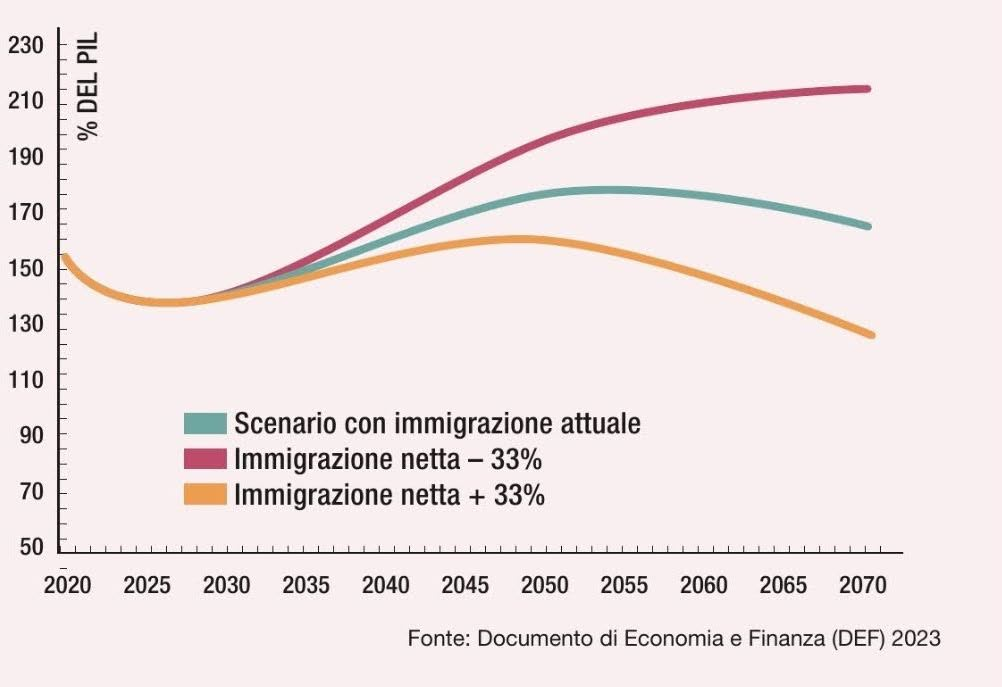
\includegraphics[width=0.95\linewidth]{images/Libro-img057.jpg}
\end{figure}

Secondo il ministero dell'Economia, un aumento della speranza di vita può ridurre la crescita del debito pubblico di 6 punti percentuali. Al contrario, una diminuzione della fertilità potrebbe far crescere il debito di circa 10 punti percentuali entro il 2070. Un aumento del 33\% dell'immigrazione potrebbe ridurre il debito pubblico rispetto al PIL di 35 punti percentuali nel 2070, mentre una diminuzione del 33\% degli immigrati potrebbe farlo aumentare di circa 45 punti.

L’immigrazione, inoltre, non è solo una questione di numeri o di impatto economico, ma riflette anche squilibri legati allo sfruttamento delle risorse nei Paesi d’origine, in cui l’Occidente ha avuto un ruolo determinante.

\subsubsection{Immigrazione e lavoro}
Confrontando i dati sui salari, occupazione\endnote{\raggedright\url{http://www.voxeu.org/article/how-immigrants-and-job-mobility-help-low-skilled-workers}} è stato notato che l'immigrazione non comporti perdite di posti di lavoro significative né riduzioni salariali diffuse per la forza lavoro locale. Gli impatti, positivi o negativi, sono generalmente lievi e localizzati\endnote{\raggedright\url{http://www.nber.org/papers/w21123}} \endnote{\raggedright\url{http://www.voxeu.org/article/immigration-trade-and-productivity-services}} \endnote{Burchardi et al., 2020\raggedright\url{https://papers.ssrn.com/sol3/papers.cfm?abstract_id=3582182}} \endnote{Penn Wharton Budget Model, 2016 \raggedright\url{https://budgetmodel.wharton.upenn.edu/issues/2016/1/27/the-effects-of-immigration-on-the-united-states-economy}} \endnote{Longhi et al., 2004 \raggedright\url{https://ideas.repec.org/p/wai/pscdps/dp-47.html}}.

Oltre che essere lavoratori, consumatori e contributori gli immigrati possono diventare imprenditori e creare nuovi
posti di lavoro.
Secondo fonti recenti, in Italia circa il 10\% delle imprese (in numero) è gestito da imprenditori stranieri.
Gli stranieri in Italia, sia imprenditori che dipendenti, producono un PIL di 139 miliardi di euro all'anno, quasi il 9\% del
totale. Quindi grazie all'imprenditorialità straniera si generano 1,2 nuovi posti di lavoro. 

Tito Boeri, ex presidente dell'INPS, Durante un intervento alla Camera dei Deputati nel 2018, affermò che:

“Senza immigrati l’INPS sarebbe in grossa difficoltà. I contributi versati dagli immigrati regolari sono fondamentali per sostenere il sistema pensionistico italiano.”

Ci sono poi diversi casi di lavoratori stranieri che vengono assunti in nero: una condizione che impedisce loro di contribuire regolarmente al sistema previdenziale. Tuttavia, questa responsabilità ricade principalmente sul datore di lavoro, non sul lavoratore stesso.

Nel dibattito pubblico, l’espressione “migranti economici” viene spesso usata in modo distorto, con l’intento di sminuire o delegittimare chi emigra per migliorare le proprie condizioni di vita. Si suggerisce che queste persone non fuggano dalla povertà, ma siano mosse dall’avidità o da un desiderio di arricchimento.
Ad esempio, se una persona davanti al supermercato chiede qualcosa da mangiare e tu le offri del cibo, ma lei ti risponde che preferisce dei soldi, non significa necessariamente che stia mentendo o approfittando. Magari ha già ricevuto abbastanza cibo durante la giornata e ora ha bisogno di soldi per pagare il gas, la luce, le bollette o l’affitto.

Tornando ai migranti economici, non è forse la stessa dinamica che porta molti occidentali a trasferirsi all’estero in cerca di migliori opportunità? Perché, allora, un italiano che emigra per lavoro viene visto come un “cervello in fuga” o una persona ambiziosa, mentre un immigrato viene spesso visto come un invasore o un approfittatore? Difficilmente qualcuno rischierebbe la vita in un viaggio estremo se non è spinto da condizioni intollerabili. Etichettarli come 'migranti economici' è riduttivo e spesso ingiusto.
Inoltre le attività economiche delle potenze occidentali, come l’estrazione di materie prime in queste regioni, possono contribuire a condizioni socio-economiche che favoriscono i flussi migratori.

\subsubsection{Immigrazione e sicurezza}
Più di un italiano su tre dichiara di percepire una bassa sicurezza nella zona in cui abita e, questa percezione è dovuta anche
all'immigrazione che in Italia ha visto u aumento nel corso degli anni\endnote{\raggedright\url{https://public.tableausoftware.com/views/denunce-2016/Dashboard7?:embed=y\&:toolbar=no\&:display\_count=no\&:showVizHome=no}}.

La gente teme che l'aumento d'immigrazione possa portare a dei problemi di
ordine pubblico e, anche in questo caso, possiamo chiedere aiuto ai dati per vedere se dal 2014 ci sono stati aumenti
di crimini.

Grazie al lavoro dell'Istat\endnote{\raggedright\url{http://dati.istat.it/index.aspx?queryid=3846} } possiamo vedere
che non abbiamo avuto un aumento della criminalità in generale, anzi, crimini diffusi tra cui furti e danneggiamenti
sono in calo, in aumento invece le truffe informatiche su cui però non possiamo trovare una correlazione con
l'immigrazione\endnote{\raggedright\url{https://public.tableau.com/views/denunce-2016/Dashboard6?:embed=y\&:display\_count=n\&:toolbar=n\&:origin=viz\_share\_link}}.

Va però ricordato che stiamo analizzando le denunce, non i reati realmente commessi, le motivazioni per cui le due cose
non vanno di pari passo sono molteplici, ad esempio come nella corruzione, riciclaggio, spaccio, i soggetti coinvolti,
da entrambe le parti non hanno vantaggi a denunciare il reato, o per un crimine troppo piccolo, sfiducia nelle forze
dell'ordine, sottostima del crimine e, la vergogna come nel caso di violenze sessuali.

\begin{mdframed}[linewidth=1pt]
Senza il denaro contante, la corruzione economica diventerebbe più complessa. Le alternative possibili sarebbero principalmente tre:

\begin{itemize}
\item Criptovalute e valute digitali: se utilizzate in modo anonimo — ad esempio tramite mixer o wallet non soggetti a procedure KYC (Know Your Customer) — possono svolgere un ruolo simile al contante.
\item Beni di lusso e scambi in natura: oggetti di valore come orologi, automobili, opere d’arte, oppure favori personali come assunzioni, incarichi o altri vantaggi non monetari, possono essere usati per trasferire valore in modo non tracciabile.
\item Fatture gonfiate e consulenze fittizie: si ricorre a strumenti legali in apparenza, come servizi professionali simulati o costi artificiosamente elevati, per mascherare pagamenti illeciti.
\end{itemize}
\end{mdframed}

Aumentando le persone in un paese, possono aumentare anche le possibilità di crimine, ma allo stesso modo, potrebbe succedere anche con un incremento della
natalità, incoraggiata dallo stato.

La percezione del numero totale di migranti può risultare deformata, infatti la percentuale di immigrati in Italia è del 9\%, una delle più basse in Europa, ma i sondaggi di Ipsos-Mori indicano che viene invece percepita come del 26\%, mentre la disoccupazione percepita al 49\% quando
in realtà è al 12\%\endnote{\raggedright\url{https://www.ipsos.com/ipsos-mori/en-uk/perceptions-are-not-reality-things-world-gets-wrong}}.

Quando si hanno molti dati possono essere usati per favorire una narrazione e non sempre è semplice notare la forzatura.
Ecco un esempio: Gli immigrati nelle carceri italiane sono 32\% mentre sul territorio sono circa il 9\%. Quindi gli immigrati delinquono più degli italiani.

Associare carcere e criminalità è un'idea intuitiva, ma a noi non interessa sapere chi c'è dentro il carcere. A noi interessa sapere se gli stranieri sono un problema per la sicurezza. Quindi perché non cercare direttamente informazioni sulla criminalità invece di portare dati sulle carceri?

Questo grafico mostra come negli ultimi 15 anni la criminalità in Italia continui a diminuire.

\needspace{4cm}
\begin{figure}[H] 
\centering
\floatsetup{valign=c}
\begin{subfigure}[b]{0.48\textwidth} 
\begin{tikzpicture}
\begin{axis}[
    xmin=2006, xmax=2020,
    ymin=0, ymax=3000000,
    xtick={2006,2008,...,2020},
    ytick={0,500000,1000000,1500000,2000000,2500000,3000000},
    xticklabel={\pgfmathprintnumber[int trunc]{\tick}}, 
    xticklabel style={rotate=45},
    legend style={at={(0.5,-0.15)},
    anchor=north,legend columns=-1},
    ymajorgrids=true,
    grid style=dashed,
    axis x line*=bottom, 
    axis y line*=left, 
    every axis x label/.style={at={(current axis.right of origin)},anchor=north west},
    every axis y label/.style={at={(current axis.above origin)},anchor=north east},
    scaled x ticks=false,
]
\addplot[
    color=blue,
    mark=square,
    ]
    coordinates {
    (2006,2771490)(2007,2933146)(2008,2709888)(2009,2629831)(2010,2621019)(2011,2763012)(2012,2818834)(2013,2892155)(2014,2812936)(2015,2687249)(2016,2487389)(2017,2429795)(2018,2371806)(2019,2301912)(2020,1900624)
    };
\end{axis}
\end{tikzpicture}
\caption{Denunce totali - Istat \raggedright\url{http://dati.istat.it/Index.aspx?DataSetCode=dccv_delittips}}
\label{fig:grafico1}
\end{subfigure}
\hfill
\begin{subfigure}[b]{0.48\textwidth} 
\begin{tikzpicture}
\begin{axis}[
    xmin=2006.5, xmax=2019.5, 
    ymin=0, ymax=350000,
    xtick={2006,2008,...,2020},
    ytick={0,50000,100000,150000,200000,250000,300000,350000},
    xticklabel={\pgfmathprintnumber[int trunc]{\tick}}, 
    xticklabel style={rotate=45}, 
    legend style={at={(0.5,-0.15)},
    anchor=north,legend columns=-1},
    ymajorgrids=true,
    grid style=dashed,
    axis x line*=bottom, 
    axis y line*=left, 
    every axis x label/.style={at={(current axis.right of origin)},anchor=north west},
    every axis y label/.style={at={(current axis.above origin)},anchor=north east},
    scaled x ticks=false, 
]
\addplot[
    color=blue,
    mark=square,
    ]
    coordinates {
    (2007,303339)(2008,302583)(2009,276481)(2010,274697)(2011,283508)(2012,290534)(2013,306840)(2014,308617)(2015,309373)(2016,261421)(2017,264197)(2018,279018)(2019,265061)(2020,241016)
    };
\end{axis}
\end{tikzpicture}
\caption{Denunce stranieri - Istat \raggedright\url{http://stra-dati.istat.it}}
\label{fig:grafico2}
\end{subfigure}
\label{fig:grafici_affiancati}
\end{figure}

Ma quindi come mai la popolazione carceraria non decresce allo stesso modo?

La popolazione carceraria non è uguale alla popolazione che ha infranto la legge. Anche escludendo i reati che non
prevedono la detenzione, dal conteggio sono comunque esclusi gli individui che hanno avuto accesso a misure alternative di
detenzione, come lavori socialmente utili o gli arresti domiciliari. Gli stranieri che riescono ad ottenere queste
misure alternative sono una minoranza, in quanto a volte non riescono a soddisfare i requisiti, come un domicilio o un lavoro stabile ecc…

Un'ulteriore problema è che guardare solamente il numero di carcerati non dice nulla sul reato commesso. Secondo dati Istat\endnote{\raggedright\url{https://www.istat.it/it/files/2015/03/detenuti-2015-1.pdf}} gli stranieri sono molto presenti per reati che vanno da zero a cinque anni mentre per reati maggiori troviamo più italiani.

In Italia esiste il reato di clandestinità che un italiano non potrà compiere. 
Questi sono solo alcuni esempi per dire che anche un dato vero, potrebbe non essere il corrispettivo del fenomeno che si vuole indagare e, suonando come ragionevole, risulta difficile non crederci.

Per comparare meglio queste due popolazioni, potremmo farlo meglio dividendo tra immigrato regolare, quindi con gli stessi diritti di un italiano e, immigrato irregolare. Un immigrato irregolare non ha il diritto di lavorare, quindi quelli più
bravi lavoreranno in nero. Ma in situazioni di estrema difficoltà, la sopravvivenza e la ricerca di mezzi di sussistenza possono spingere le persone a muoversi nell'illegalità, quando le alternative legali sono precluse o insufficienti. Così il reato di immigrazione è spesso legato ad altro, che può andare dal lavoro in nero, fino allo spaccio. 

Sarebbe interessante trovare il dato che differenzi gli immigrati in regolari e irregolari ma non è facile. Alcuni studi
(Crocitti, 2014\endnote{\raggedright\url{https://www.oxfordhandbooks.com/view/10.1093/oxfordhb/9780199859016.001.0001/oxfordhb-9780199859016-e-029}}) osservano come la percentuale dei migranti irregolari nelle carceri vari tra il 60 e l'80\% a
seconda del tipo di crimine. Secondo la ricerca sulla criminalità del Centro Studi e Ricerche Idos (F. Pittau, S.
Trasatti 2009) nel 2005 in Italia di 550.590 denunce solamente il 37.709 erano di stranieri regolari, quindi solo il
6.84\%\endnote{Marie - Pinotti, 2024\raggedright\url{https://www.aeaweb.org/articles?id=10.1257/jep.38.1.181}} \endnote{\raggedright\url{https://www.cambridge.org/core/journals/british-journal-of-political-science/article/terrorism-and-migration-an-overview/2D92D099D870D7D8E606C39E683D3E89}}.

Ma perché allora non si mettono in regola gli immigrati? 

Un primo problema l'abbiamo all'arrivo, molti migranti non hanno documenti o permessi per viaggiare legalmente in aereo perché difficile ottenere un visto dal paese di destinazione, costringendoli a tentare altre vie più pericolose. Quindi, sebbene possano acquistare un biglietto aereo, potrebbero essere intercettati dalle autorità di immigrazione all'aeroporto e respinti. Questo può portare i migranti a muoversi senza documenti d'identità, per paura di essere riconosciuti ed espulsi.

A marzo 2021 in Italia sono state registrate 207 mila domande di regolarizzazione, ma di queste soltanto 1.480 sono
giunte nella fase conclusiva: lo 0,7\% del totale. Anche una volta ottenuto il permesso, quando sarà scaduto ci si
potrebbe trovare nella condizione di averne diritto ma l'attesa renderà irregolare questa persona
per un certo periodo di tempo. Inoltre l'immigrazione è regolata con la legge Bossi Fini, fatta molti anni fa, quando il fenomeno era molto diverso,
che prevede l'ingresso di persone che abbiano già un contratto lavorativo prima di arrivare in Italia, un
requisito molto difficile da ottenere senza un colloquio di persona e senza conoscere bene la lingua. 
Lo scrupolo burocratico per mantenere la sicurezza dello stato, rischia di ottenere l'effetto opposto.

La regolarizzazione porterebbe nelle casse dello Stato 1,2 miliardi di euro, tra Irpef e contributi previdenziali. 

Anche per i minori, non esistendo agli occhi dello
stato, quando spariscono diventa quasi impossibile ritrovarli, rischiando di finire nelle reti dello spaccio e della prostituzione.
Semplificare la messa in regola degli stranieri, li può sottrarre da una vita pericolosa, importante sia per il
benessere delle persone e della comunità. 

Infine sul piano sociale, l'immigrazione arricchisce il tessuto culturale, introducendo nuove prospettive e tradizioni che possono rivitalizzare le società. Se all'inizio l'integrazione può presentare ostacoli e generare tensioni, come discusso nello studio "Public attitudes towards migrants: understanding cross‐national and individual differences"\endnote{\raggedright\url{https://pmc.ncbi.nlm.nih.gov/articles/PMC7801858/}}, nel corso del tempo gli immigrati e i loro discendenti tendono ad assimilare la lingua, i valori e le norme del paese ospitante, diventando membri attivi e contributivi della comunità. Non solo, i figli degli immigrati spesso abbracciano ideali progressisti, talvolta influenzando positivamente il panorama politico e contribuendo a plasmare politiche più inclusive e socialmente orientate, come evidenziato in  "Long-term political consequences of immigration: Voting preferences of immigrants’ children in European countries"\endnote{CEPR, 2022 \raggedright\url{https://cepr.org/voxeu/columns/long-term-political-consequences-immigration-voting-preferences-immigrants-children}}.

\begin{mdframed}[linewidth=1pt]
Il termine "buonismo" viene talvolta utilizzato per descrivere un atteggiamento considerato eccessivamente tollerante, adottato allo scopo di apparire virtuosi. Tuttavia, questo concetto non si applica automaticamente a ogni posizione contraria alla nostra. Chi nasce in un Paese con maggiori risorse e infrastrutture, come l’Italia, parte da condizioni di vantaggio rispetto a chi nasce in contesti più svantaggiati. Questa disparità non è frutto del merito individuale, ma di circostanze casuali. Di conseguenza, sostenere la necessità di pari opportunità non è una questione di buonismo, ma di riconoscimento di una disuguaglianza. L’obiettivo dovrebbe essere quello di garantire condizioni di partenza più eque per tutti.
\end{mdframed}

\subsubsection{Wokeism}
Il termine “wokeism” (in italiano “wokismo”) nasce con un’accezione positiva: descrive la consapevolezza e la sensibilità verso le ingiustizie sociali e politiche, come il razzismo, le discriminazioni di genere e le disuguaglianze sistemiche. Nel tempo, tuttavia, questo concetto si è caricato di sfumature critiche. In certi contesti, viene oggi impiegato per indicare un atteggiamento percepito come eccessivamente radicale, autoreferenziale o divisivo. Si tratta di un’evoluzione semantica significativa, che merita attenzione: movimenti nati con l’intento di promuovere inclusione possono, in alcune loro manifestazioni, finire per enfatizzare le differenze al punto da creare nuove forme di separazione.

Tradizionalmente, molte lotte sociali, in particolare quelle sostenute da movimenti progressisti, si sono fondate su una visione universalista. L’obiettivo era coinvolgere l’intera società in un processo di cambiamento, al di là delle identità individuali. La battaglia contro il razzismo, ad esempio, non veniva intesa come esclusiva delle persone nere, ma come una causa comune. Emblematico, in questo senso, è l’esempio della Marcia su Washington del 1963, guidata da Martin Luther King Jr., in cui persone bianche e nere marciarono fianco a fianco per i diritti civili.

Una componente più identitaria dell’attuale attivismo, tuttavia, propone una prospettiva differente: l’idea che la legittimità di parlare su certe tematiche dipenda strettamente dall’esperienza personale di discriminazione. In questa visione, solo le persone nere possono affrontare il tema del razzismo, solo le persone LGBTQ+ discutere delle questioni che le riguardano, solo le donne parlare di femminismo. Questo approccio nasce da esperienze concrete di esclusione, spesso aggravate da paternalismo e appropriazione indebita del discorso da parte di chi non ne ha vissuto le conseguenze. Tuttavia, se applicato rigidamente, può escludere interlocutori potenzialmente alleati e ostacolare un dialogo più ampio ed efficace.

In una società che aspira all’inclusività, l’obiettivo dovrebbe essere quello di avvicinare chi è ancora distante da certe sensibilità, non di allontanarlo. Il valore di un’idea risiede nella sua capacità di convincere, nella coerenza e nella forza delle sue argomentazioni, non nell’identità di chi la enuncia. Così come un critico cinematografico non deve necessariamente essere un regista per esprimere un parere fondato, allo stesso modo è possibile contribuire a una causa anche senza far parte del gruppo direttamente interessato.

È altrettanto importante riconoscere che molte rivendicazioni nascono da ferite ancora aperte e da un lungo processo di marginalizzazione. Tuttavia, una risposta costruita sulla contrapposizione identitaria rischia di replicare dinamiche di esclusione simili a quelle che si vorrebbero superare. Laddove si afferma una gerarchia morale fondata sull’identità, si corre il rischio di reintrodurre schemi chiusi, che non favoriscono il confronto e rendono difficile il cambiamento.

Alcuni episodi recenti evidenziano questa tensione. In alcune manifestazioni femministe, ad esempio, si sono adottate pratiche simboliche come la divisione tra uomini e donne nei cortei, con le donne in testa e gli uomini in coda. Sebbene il gesto abbia un valore simbolico chiaro, dare centralità alle protagoniste della lotta, può trasmettere un messaggio ambiguo, che sembra instaurare una gerarchia nella partecipazione. Anche nel simbolismo, è importante che il messaggio resti inclusivo e coerente con l’ideale di parità.

La legittimità del discorso non può essere ancorata unicamente all’identità. Quando si adottano criteri rigidi di appartenenza per definire chi può o non può esprimersi, si rischia di assorbire inconsapevolmente elementi tipici di logiche ideologiche identitarie che, storicamente, sono state utilizzate per escludere. Il sospetto verso chi dissente, l’ossessione per la purezza ideologica e la chiusura verso il diverso sono atteggiamenti che possono affiorare anche in contesti che si definiscono progressisti. Il fatto che un’ideologia si presenti con un linguaggio inclusivo non la rende automaticamente immune da derive dogmatiche.

Un caso spesso citato è la metafora proposta da Michela Murgia: “Nascere maschi in un sistema patriarcale e maschilista è un po' come essere figli maschi di un boss mafioso.” Si tratta di un’immagine potente, pensata per stimolare una riflessione sul ruolo della passività e della complicità involontaria nei sistemi di potere. Tuttavia, se interpretata in modo assoluto, questa metafora può suggerire l’idea di una colpa ereditaria e ineluttabile, lasciando poco spazio a percorsi individuali di consapevolezza e cambiamento. Una lettura rigida rischia di trasformare il discorso in una forma di moralismo che alimenta senso di colpa più che responsabilità attiva.

\begin{mdframed}[linewidth=1pt]
Il diritto delle donne a non diventare madri contro la propria volontà è una conquista fondamentale del femminismo. La legge italiana tutela questa autonomia riconoscendo, ad esempio, la possibilità di non riconoscere il bambino alla nascita e lasciarlo in ospedale in anonimato (DPR 396/2000), una misura essenziale in situazioni di vulnerabilità.
Questa protezione nasce dalla consapevolezza che donne e uomini sono diversi, anche biologicamente. Per questo è giusto che esistano tutele specifiche per le donne, come il divieto di licenziamento in gravidanza, perché gli uomini, per ovvie ragioni, non vivranno mai quella condizione. Queste misure non creano disparità, ma servono a riequilibrare le differenze di partenza.
Tuttavia, proprio in nome dell’equità, è importante riflettere su una disparità ancora poco discussa: se la donna decide di proseguire la gravidanza anche contro il volere dell’uomo, quest’ultimo non ha alcuno strumento legale per rifiutare la paternità. Al contrario, può essere riconosciuto come padre con sentenza, anche contro la sua volontà, e obbligato a contribuire economicamente al mantenimento del bambino, anche con prove genetiche. Il rifiuto agli esami può essere usato come indizio a suo sfavore.
La legge nasce per tutelare il diritto del minore, e questo è sacrosanto. Tuttavia, si può rilevare un'asimmetria normativa: mentre lo Stato prevede la possibilità per la madre di non riconoscere il bambino alla nascita, proteggendo così la sua autonomia e garantendo la tutela del minore, non esiste un analogo strumento legale che consenta all'uomo di rifiutare la paternità prima della nascita, neppure in situazioni complesse come quelle derivanti da inganni (es. manomissione di contraccettivi\endnote{\url{https://www.salute.gov.it/portale/donna/dettaglioContenutiDonna.jsp?id=1011&area=Salute\%20donna&menu=nascita}} \endnote{\url{https://www.laleggepertutti.it/91330_figlio-da-coppia-non-sposata-se-un-genitore-non-vuol-riconoscere-il-bambino}}). La legge non tutela nessuno dei due sessi da questo tipo di raggiri, che possono colpire tanto uomini quanto donne.
Il femminismo ha lottato per liberare le donne dalla maternità forzata. Estendere questo principio anche agli uomini non è maschilismo, ma un tentativo di perseguire una maggiore coerenza. Non si tratta di negare tutele alle donne, ma di chiedere parità di libertà e di responsabilità per entrambi i genitori, nel rispetto delle differenze.
Una genitorialità ideale, in un contesto di parità, si fonda sulla scelta condivisa e consapevole di entrambi i partner, evitando imposizioni legali unilaterali, pur riconoscendo il ruolo della legge nel tutelare i diritti fondamentali del minore. Quando non c’è consenso reciproco, dovrebbe essere chi sceglie di diventare genitore ad assumersene il carico, o in alternativa, lo Stato, assecondando la giustizia riproduttiva e parità tra i sessi, non in contrapposizione, ma in alleanza.
\end{mdframed}

È essenziale distinguere tra la legittimità dell’esperienza soggettiva e la sua elevazione a criterio assoluto di giudizio. Ogni interpretazione parziale della realtà rischia di diventare distorsiva se non è accompagnata da apertura al confronto e da un riscontro empirico più ampio. È come guardare il mondo da una piccola finestra e credere che quello sia tutto il mondo.

Questo schema mentale, che si ritrova in varie forme di discriminazione, dal razzismo all’omofobia, dalla misoginia alla misandria, comporta un significativo impoverimento del pensiero critico. Si tratta di una logica che riduce l’individuo alla sua appartenenza, annullando la complessità della sua storia personale: i percorsi di crescita, le difficoltà superate, le responsabilità assunte, le scelte compiute, le occasioni in cui ci si è messi in discussione.

Secondo questa visione, qualsiasi sforzo di autodeterminazione rischia di essere vanificato da una classificazione identitaria rigida, dal genere, al paese o perfino al segno zodiacale. È un approccio che esclude a priori e non ammette possibilità di trasformazione.

Ogni etichetta è una semplificazione. La bontà di un’idea non dipende dalla sua autodefinizione, ma dai suoi effetti e dalla sua apertura al confronto. Anche ideologie autoritarie si sono presentate come “democratiche” (Corea del Nord). Come ricorda Umberto Eco ne Il fascismo eterno\endnote{\raggedright\url{https://www.amazon.it/dp/8893442418}}, l’autoritarismo può indossare molte maschere, anche quelle apparentemente progressiste. Per questo, la vigilanza critica non può essere prerogativa di una parte sola.

Anche quando si trattano temi culturali complessi, è utile evitare spiegazioni riduttive. È vero che le donne subiscono una pressione estetica maggiore, ma è altrettanto vero che il giudizio proviene anche da altri soggetti femminili. La mercificazione del corpo femminile coinvolge più attori, anche inconsapevoli. Dinamiche come l’ottenimento di vantaggi attraverso il fascino fisico non vanno banalizzate né moralizzate, ma riconosciute come parte di un sistema che tende a premiare certi comportamenti.

Analogamente, esistono doppi standard poco analizzati. Una donna che dichiara di preferire uomini alti non viene generalmente criticata; un uomo che esprime una preferenza per donne magre può invece essere accusato di superficialità. Questo esempio non vuole negare le disuguaglianze che colpiscono le donne, ma suggerire la necessità di un’analisi più equilibrata e coerente anche all’interno dei movimenti di critica sociale.

In un contesto di crescente attenzione alle identità, la tentazione di definire se stessi attraverso etichette rigide è forte. Tuttavia, in alcuni casi, proprio la fluidità identitaria e la libertà dal bisogno di etichettarsi possono aprire nuovi spazi di autenticità. L’adesione a un’ideologia, per quanto giusta nelle sue intenzioni, non dovrebbe mai trasformarsi in una gabbia all'interno della quale le nostre idee faticano a sfuggire.

Anche sul piano culturale e mediatico, alcune forzature rischiano di compromettere l’efficacia comunicativa. Negli anni ’90, molte opere inserivano personaggi appartenenti a minoranze in modo spontaneo e narrativamente coerente. Serie come La Tata, Willy, il principe di Bel-Air, I Robinson, Buffy, Xena o 8 sotto un tetto presentavano donne forti, persone nere senza che la loro identità fosse il centro della narrazione. Questi elementi, da soli, non determinano la qualità di un film. La sua riuscita dipende soprattutto dalla recitazione, dalla regia, dalla trama e da altri aspetti artistici fondamentali. L’inclusione funzionava perché parte integrata del racconto, non c'erano forzature.
Una narrazione ben costruita ci permette di immergerci nella storia anche senza identificarci direttamente con i personaggi, anche se questi non condividono con noi caratteristiche superficiali come sesso, orientamento sessuale, colore della pelle e così via. Anzi, è proprio questa distanza a rappresentare la vera ricchezza del racconto: se una storia parla esattamente di te, senza offrirti prospettive nuove, allora sarà difficilmente arricchente.

Un caso letterario emblematico si è verificato nel 2021, quando il Premio Planeta è stato assegnato a Carmen Mola, autrice di romanzi noir noti per le protagoniste femminili forti e l’approccio a tematiche sociali complesse. Durante la cerimonia, si è scoperto che dietro lo pseudonimo si celavano in realtà tre autori spagnoli: Jorge Díaz, Agustín Martínez e Antonio Mercero. La rivelazione ha generato un ampio dibattito, sollevando interrogativi sull’impatto che l’identità dell’autore può avere sulla ricezione di un’opera. 

Infine, è importante ricordare che la colpevolizzazione difficilmente produce cambiamento: irrigidisce le posizioni e indebolisce il dialogo. Le battaglie sociali non si impongono: si condividono, si costruiscono insieme. L’urgenza morale non può sostituire la necessità di persuasione. Chi non partecipa a una determinata lotta non è necessariamente complice: può essere impegnato su altri fronti altrettanto validi.

Se è vero che statisticamente uomini e donne mostrano propensioni diverse, è altrettanto vero che qualità come forza, empatia, determinazione o cura non hanno genere. Attraverso la collaborazione, persone con esperienze e caratteristiche diverse possono contribuire in modo complementare al progresso della collettività. Invece di screditare le differenze altrui, sarebbe più costruttivo riconoscere e valorizzare le peculiarità di ciascuno, mettendole a disposizione degli altri in una prospettiva di cooperazione e condivisione.

\begin{mdframed}[linewidth=1pt]
Quando satira, ironia e black humor vanno oltre?

A volte è difficile fare qualcosa di divertente senza offendere qualcuno. Anche uno scherzo ad un amico spesso, almeno
in maniera minima, punta a creare un fastidio/lesione, perché si spaventa, perché viene bagnato, perché gli nascondiamo qualcosa ecc… La satira e
il black humor utilizzano spesso elementi di comicità che si basano sul ledere qualcosa. Queste modalità comiche sono
le più rischiose perché vanno a toccare argomenti su cui l'opinione pubblica è più sensibile, come
guerra, disabilità, morte, malattia, orientamento religioso, sessuale, discriminazioni razziali, di genere, violenze
sessuali anche su minori. Non è un caso che le tematiche siano così sensibili, perché uno degli scopi della satira è
proprio quello di portare le persone a ragionare su certi temi, usando la comicità come pretesto per arrivare ad un
pubblico più vasto. Un altro degli obiettivi che si prefigge la satira è quello di stemperare e cercare di portare un
sorriso anche nel dramma. La satira e il black humor cercano di sovvertire il perbenismo, il politicamente corretto, il
bigottismo e tutto ciò che culturalmente è sempre stato un tabù. Tutto ciò che è soggettivo o che culturalmente non si
può toccare la satira va a toccarla apposta. Quasi come un esercizio atto a liberarsi da questa morale che ci dice in
cosa credere, cosa è giusto e cos'è sbagliato, in maniera cieca senza possibilità di rimetterla in discussione. 

Ma quando questa comicità si spinge oltre? Il fatto che qualcuno si senta offeso non può essere l'unico metro di giudizio,
specialmente in questo periodo, lo possiamo vedere sulla rete, la gente si offende per tutto, sia che si critichi una
squadra di calcio fino al beniamino della serie TV. Quindi per qualcuno satira e black humor sono una modalità di
espressione che non deve avere limiti.

Dall'altro lato si usa il black humor in maniera un po' furba in alcuni casi e
un po' pavida negli altri. Su internet circolano meme di Black humor dove però al loro interno non sono presenti elementi comici, rimanendo così solo il black. Questo tipo di tentato umorismo cerca di degradare e
deridere la sofferenza altrui. In questi casi la domanda che sorge spontanea è: perché senti il bisogno di svilire
qualcuno gratuitamente? Se non c'è umorismo, non c'è una critica sociale, cosa resta? Mancano gli elementi umoristici che possono essere giochi parole, situazioni paradossali, doppi sensi, ironia ecc… Sono solo un insieme
di termini culturalmente mal visti che orbitano attorno alla discriminazione sessuale, di genere, razziale o religiosa. Ma senza almeno un elemento comico cosa resta? Il tranello a questo punto prevede che se non ridi è colpa tua perché sei un boomer, un bigotto, una persona triste, uno senza umorismo ecc… non perché la battuta non fa ridere.
Gli stratagemmi per porsi superiori agli altri sono tanti, uno di questi è il termine cringe, che come il back humor, a volte nasconde le cose che vogliamo allontanare, su cui siamo più fragili e ci imbarazzano, riducendolo a meme per fare finta di averne preso le distanze.

Altre volte si vuole insultare una persona o un gruppo e, quando gli altri si arrabbiano ci si mette in salvo con la scusa: era solo una battuta!

Se un cantante, un film o un videogame parla di violenza, come per la satira, si ha un contesto dove si sa che quel messaggio ha uno scopo di intrattenimento o di denuncia ma che non rappresenta l'idea del suo creatore. Anzi, spesso il suo creatore la pensa esattamente nel modo opposto. Quando ci sono dei troll online, in tv o nella radio il discorso cambia. Persone che divulgano messaggi pericolosi ora sono potuti venire allo scoperto con il trolling, perché in questo modo hanno un ancora di salvataggio, possono dire che loro non la pensano così, stavano solo trollando, rendendo più difficile distinguere critica sociale dall'abuso.
Anche qua, il fatto che qualcuno si diverta a offendere la gente invece che farla ridere, dice più di loro che di chi stanno attaccando.
Idealmente la satira punta a stimolare una riflessione critica, quello è uno degli scopi, anche se qualcuno potrebbe rimanere offeso.

Bisogna chiedersi: cos'è che c'è di divertente? Qual è l'elemento comico oltre al lessico e al toccare tematiche sensibili? Se non si riesce a trovare un motivo, allora forse sono stati gli altri a dirci che è
divertente e, noi stiamo solo ripetendo questo messaggio. E così ridiamo della morte, delle guerre e delle malattie riducendoli a meme, credendo di emanciparci ma finendo talvolta per conformarsi. Quando la satira non ha un messaggio di denuncia, spesso la usiamo per tentare di esorcizzare
qualcosa che ci spaventa ma con l'effetto di svilire qualcosa di importante che ci riguarda. A volte ridiamo di un meme
tragico, per non affrontare quanto quella cosa abbia a che fare con noi. Detto questo non voglio demonizzare il meme o il black humor, come credo che si sia già intuito, ma se reagiamo come reagirebbero tutti, rischiamo ancora una volta di non essere autentici.

La satira come detto può essere uno strumento per ridimensionare le persone mettendole davanti alle proprie idiosincrasie. Ma cosa vogliamo ottenere? Ne vale la pena? Rischiamo di compromettere il rapporto o far rimanere male qualcuno per qualcosa di poco conto? Mettere sempre in ridicolo gli altri e, senza utilizzare questo come pretesto per denunciare cose importanti, che senso ha? Se metti sempre e tutto in ridicolo cos'è importante per te? Sembra quasi di scappare dalle questioni che ad un certo livello non ci fanno stare sereni.
Il meme o la satira, mi porta a capire qualcosa? Avvicinandomi di conseguenza a quell'oggetto di discussione che solitamente crea frizione? O lo uso per prendere in giro e di conseguenza allontanarmici? Muoiono persone in un incidente o una guerra: rido per esorcizzare che questo a me non capiterà? o per far vedere che io sono uno tutto di un pezzo e che non sono così sensibile? perché in generale fai quel che fai?

Se troppo spesso il dibattito pubblico sembra un meme continuo, non stupisce se anche noi per primi discutiamo in questo modo.

Una battuta fatta ad un gruppo di amici o ad un pubblico più vasto che può essere uno spettacolo dal vivo, la TV, la
carta stampata o i social network deve avere un attenzione diversa. Se facciamo una battuta razzista e i nostri amici sanno che non lo siamo, ha un peso diverso
rispetto ad una battuta fatta da un razzista o uno di cui non conosciamo le sue poizioni. Poi uno potrebbe dire: non è affar mio se questa persona si
offende perché legata a delle vecchie idee culturali di cosa si può dire e cosa no. Ma la domanda è sempre quella: qual è il tuo obiettivo? Farlo ridere? O rovinare il vostro rapporto? Ne vale la pena?

Dietro ad una battuta spesso ci sono ore di studio per trovare il giusto equilibrio tra ironia e spunti di riflessione. Con questo non possiamo limitare l'umorismo ai soli professionisti, ma sarebbe preferibile che qualsiasi battuta ironica fosse frutto di un'elaborazione volta a evitare fraintendimenti. Anche qua è giusto chiedersi: ne vale la pena? Il messaggio che voglio dare è abbastanza importante da giustificare l'ira di qualcuno? Questa battuta potrebbe portare più persone a ridere o a riflettere rispetto a quelli che invece farò arrabbiare?

Tanto dipende da chi è a fare humor. Se un nero fa una battuta sul razzismo è meno probabilme che qualcuno etichetti il comico come razzista rendendo più chiara l'ironia. Mentre se un bianco insiste con battute sui neri, può nascere un sospetto sulla sua possibile intenzione razzista.

Questo non significa che sia autorizzato a fare battute solo chi fa parte di un certo gruppo. Ma come si capisce se questa persona è ironica o cova sentimenti negativo verso il suo target? Può essere utile conoscere il
suo trascorso e cos'ha affermato o scritto negli anni in merito ai temi oggetto della sua ironia.

il fatto che si possa dire tutto non vuol dire che si debba dire tutto, c'è sempre modo e maniera -
Pif\endnote{\raggedright\url{https://www.ansa.it/puglia/notizie/2022/03/31/bifst-pif-la-satira-non-deve-essere-necessariamente-cattiva\_6e16d720-9984-489b-8b1c-6d38471ab607.html}}
\end{mdframed}

\begin{mdframed}[linewidth=1pt]
Un esempio di come le esigenze personali a volte siano contrarie a quelle sociali? Secondo dati riportati da siti commerciali per adulti come GameLink, alcuni degli Stati con legislazioni più restrittive verso i diritti LGBTQ+, come il North Carolina e il Mississippi, risultano tra quelli con un’elevata fruizione di contenuti pornografici a tematica gay o trans. Tuttavia, tali dati non provengono da fonti ufficiali e non permettono di trarre conclusioni definitive\endnote{\raggedright\url{https://www.vice.com/it/article/wdwm75/gli-stati-omofobi-sono-anche-quelli-che-scaricano-piu-porno-trans-e-gay}}.

Quindi sono pro matrimoni gay, ma per le adozioni? Qua non mi sento di esprimere una mia idea ma affidarmi a quanto scritto nel dossier\endnote{\raggedright\url{http://www.voxdiritti.it/stepchild-adoption-dagli-psicologi-un-dossier-che-dimostra-come-lomogenitorialita-non-influisca-sul-benessere-psicologico-dei-figli/}} presentato dall'Ordine degli Psicologi del Lazio contenete oltre 70 studi, svolti tra 1972 e il 2015. 

Il presidente dell'Ordine degli Psicologi del Piemonte, Alessandro Lombardo, Spiega che per la salute psicologica del
bambino non sembrano esserci problemi a crescere all'interno di una famiglia arcobaleno: "Il
vero problema nel crescere in famiglie omogenitoriali, ciò che le differenzia dalle altre famiglie, è il contesto più o
meno omofobico nel quale vivono. Questo, sì, fa la differenza. Per il resto, saranno buoni genitori, pessimi genitori,
come lo possiamo essere tutti. […] Non esiste, se non nei codici culturali, un unico modello di famiglia. È chiaro
quindi che il salto è culturale, del tipo di società che vogliamo e dobbiamo
essere"\endnote{\raggedright\url{https://www.vice.com/it/article/5gn7ba/intervista-ordine-psicologi-vendola-778}}. Inoltre legalmente un bambino può crescere con un solo genitore in casi particolari di divorzi, quindi se puo crescere bene con un solo genitore, che per forza di cose avrà un solo sesso, potrà crescere altrettanto bene con due genitori dello stesso sesso.
\end{mdframed}

\begin{mdframed}[linewidth=1pt]
Bufale sul fascismo

A volte può risultare difficile definire il fascismo in quanto non nasce da una letteratura o da una sua filosofia, ma attinge da tante idee anche contrastanti tra loro. 
Il fascismo in Italia nacque in un contesto di forte conflitto sociale, soprattutto nel periodo successivo alla Prima Guerra Mondiale (il cosiddetto Biennio Rosso, 1919-1920), caratterizzato da scioperi, occupazioni delle fabbriche e tensioni tra lavoratori e industriali.
Molti proprietari terrieri e industriali, preoccupati per la crescente influenza socialista e comunista, finanziarono e sostennero i Fasci di Combattimento di Benito Mussolini, che si distinsero per le loro azioni violente contro sindacati, lavoratori in sciopero e organizzazioni di sinistra. Persone della stessa classe sociale divise in chi combatteva contro il padrone e chi combatteva gli altri lavoratori perché foraggiati dal padrone.
Per questo guardo con un po' di sospetto i discorsi che cercando di riqualificare il fascismo distinguendolo da quello prima della guerra mondiale e quello durante e post, assumendo che prima del conflitto non fosse così male. Il mio scetticismo verso tale distinzione deriva dalla constatazione che il fascismo, fin dalle sue origini, è stato profondamente caratterizzato da un fine prevaricatorio e dalla violenza come strumento di affermazione e mantenimento del potere, aspetti che lo rendono intrinsecamente antidemocratico. Questa natura violenta e totalitaria, culminata anche nelle atrocità della guerra, è la ragione fondamentale per cui l'apologia del fascismo è vietata, al di là del solo conflitto mondiale. Mi risulta difficile, per questi motivi, pensare che un italiano possa non essere antifascista\endnote{\raggedright\url{https://www.vice.com/it/article/d3894m/bufale-storiche-sul-fascismo-mussolini-pensioni-tredicesima-terremoto}} \endnote{\raggedright\url{https://www.youtube.com/watch?v=2SkwzYjycq4}}.

\begin{itemize}
\item Mussolini ha creato le pensioni: La fonte più autorevole per conoscere la storia della previdenza sociale in
Italia è il sito dell'INPS\endnote{\raggedright\url{https://www.inps.it} } Dove possiamo trovare la voce “storia”
nel menu e leggere che sono state create nel 1898, quando Mussolini aveva 15 anni. Nel 1919
l'iscrizione alla cassa è diventata obbligatoria (3 anni prima dell'avvento
del fascismo), tuttavia la pensione sociale vera e propria viene istituita nel 1969 (24 anni dopo la morte del Duce).
La prima cassa per la malattia invece è stata creata nel è del 1947 (2 anno dopo la caduta del fascismo).
\item Mussolini ha creato la tredicesima: nel 1937 effettivamente venne introdotta la “gratifica natalizia” riservata
solo agli impiegati dell'industria e non agli operai. Per gli operai però vennero aumentate le ore
di lavoro e l'obbligo di straordinari. La tredicesima per come la conosciamo oggi, ovvero quella
estesa a tutti i lavoratori è stata introdotta dal 1960 (17 anni dopo il fascismo).
Durante un periodo storico caratterizzato dalla perdita dei diritti politici, le riforme vennero utilizzate come mezzo di controllo sociale, offrendo benefici il cui accesso era ampiamente regolato dal partito unico, come pensioni, malattia, cassa integrazione ecc… Il potenziamento dello stato sociale rappresentava anche una strategia economica chiave del regime totalitario fascista, che mirava a integrare tutti gli aspetti della vita individuale e sociale nel sistema statale e dittatoriale. Tutto passava attraverso loro, quindi o eri con loro o non avevi servizi.
\item Quando c'era lui i treni arrivavano in orario: In quanto simbolo di ordine e efficienza la
propaganda fascista puntava molto su questo punto. La stampa locale in quanto sotto regime era costretta a scrivere
questo, ma leggendo quella estera troviamo ministri e giornalisti tra cui Alexander Cockburn o George Seldes
scrivere di treni sistematicamente in ritardo e attese di almeno un quarto d'ora ai passaggi a livello.
\item Mussolini ha creato la cassa integrazione: La cassa integrazione venne attivata dal 1947, due anni dopo la morte
di Mussolini.
\item Mussolini ha fatto tanto per i lavori: Ha vietato gli scioperi, ha sciolto i sindacati e per alcune categorie di
lavoratori ha aumentato le ore di lavoro.
\item Mussolini non era razzista: Numerosi storici concordano che le leggi razziali non fossero state introdotte per
pressioni dalla Germania ma in maniera autonoma dal governo fascista.
\item Mussolini ha valorizzato le donne: Diede il voto alle donne, ma solo a un ristrettissimo numero, per poi rimuovere
questo privilegio tre mesi dopo. Fu vietato loro di partecipare a concorsi per uffici amministrativi, insegnare materie
scientifiche negli istituti tecnici, e lettere e filosofia nei licei, ne 1938 venne varata una legge che diceva che
nelle aziende dovevano esserci meno del 10\% di donne. Stupro e incesto erano solo atti contro la morale e poi normò il
matrimonio riparatore, ovvero, se stupravi una donna bastava che la sposassi per sistemare tutto.
\item Solo il fascismo ha portato il pareggio di bilancio: Successe davvero nel 1925 grazie ad Alberto De Stefani
spingendo per la liberalizzazione dell'economia, contendendo l'inflazione, riducendo la spesa pubblica e la
disoccupazione. La sua politica di "neoliberismo autoritario" era però vista di cattivo
occhio sia dalla parte più radicale del fascismo, che soprattutto da latifondisti, industriali e grandi capitalisti.
Tuttavia, queste politiche di liberalizzazione, pur avendo inizialmente portato al pareggio di bilancio, erano difficilmente sostenibili nel contesto ideologico del regime e furono presto sostituite da un'economia sempre più autarchica e bellicista, fattori che avrebbero contribuito in modo significativo al successivo declino economico del paese. Per citare un articolo\endnote{\raggedright\url{http://www.butac.it/leggende-urbane-ed-economia-fascista/} } che si è occupato di smontare questo mito, "un modello che è crollato su se stesso non è il miglior modello."
\item Mussolini ha bonificato molti territori italiani: Le bonifiche in Italia sono state avviate già precedentemente
dal governo Facta e il fascismo ne ha portate a termine solo 6\%.
\item Mussolini sconfisse la mafia: È vero che tra il 1925 e il 1929 il regime fascista avviò una campagna repressiva contro la mafia in Sicilia, guidata dal prefetto Cesare Mori, che portò all’arresto di migliaia di sospetti mafiosi e alla condanna di numerosi boss. Questa repressione fu effettivamente efficace nel breve termine e ridusse visibilmente l'influenza mafiosa. Tuttavia, le motivazioni erano più legate al controllo dello Stato che a un reale impegno antimafia, e la mafia si riorganizzò rapidamente dopo la caduta del fascismo, in parte grazie all'appoggio degli Alleati nel dopoguerra.
\item Mussolini ha fatto rispettare l’Italia nel mondo conquistando nuove terre: Le campagne coloniali italiane sotto Mussolini furono caratterizzate da inefficienza e disorganizzazione, con un uso sproporzionato di risorse rispetto ai risultati ottenuti. La guerra in Libia, durata dieci anni, fu segnata dalla violenza contro i civili, nonostante la resistenza fosse costituita da piccole bande di guerriglieri. Anche in Somalia, le azioni violente furono guidate dal desiderio di gloria personale piuttosto che da obiettivi strategici, gravando pesantemente sulle finanze statali. L'intervento in Etiopia vide l'impiego di un enorme contingente militare e l'uso di tattiche che violavano le norme internazionali sulla protezione dei civili. Queste azioni includevano il bombardamento della Croce Rossa, un atto senza precedenti volto a impedire l'assistenza agli etiopi e a nascondere le atrocità commesse. Pietro Badoglio, divenuto generale dell'esercito, fu responsabile di bombardamenti intensivi tra il 1935 e il 1936.
\item L'estrema destra ha fatto meno vittime dell'estrema sinistra: Il dibattito sulle vittime del comunismo e del fascismo richiede una distinzione tra il comunismo come ideale teorico e i regimi storici che si sono dichiarati comunisti. Nessuno stato ha mai realizzato pienamente il modello comunista previsto da Marx, che immaginava una società senza stato e senza classi. Regimi come quello di Stalin si sono invece distaccati dagli ideali marxisti, accentrando il potere, limitando le libertà e mantenendo i mezzi di produzione sotto il controllo del partito, anziché del popolo. Molti comunisti critici di Stalin sottolineano che il suo operato non rappresenta il comunismo, mentre il fascismo è solitamente definito proprio dalle azioni e dalle ideologie di figure come Hitler e Mussolini. Anche la Cina, pur governata dal Partito Comunista, mescola elementi di socialismo e capitalismo, rendendo complesso definirla pienamente comunista. Inoltre, il ruolo dell’Unione Sovietica nella sconfitta del nazismo è stato cruciale, ma deve essere considerato insieme al contributo degli Alleati occidentali, che hanno fornito supporto militare ed economico decisivo. Un’analisi equilibrata e basata su fonti solide consente di affrontare queste tematiche evitando generalizzazioni o distorsioni.
\item Mussolini ha fatto la scuola pubblica, educazione fisica, autostrade, case:

\begin{itemize}
\item La scuola pubblica nasce nel 1861 con la legge Casati 
\item L'educazione fisica viene introdotta nel 1848 e diventa obbligatoria nel 1859 
\item La prima autostrada venne creata nel 1921 dall'ingegnere Piero Puricelli (governo Giolitti)
\item La legge sulle case popolari è del 1903 del senatore Luigi Luzzanti
\item la prima cassa mutua di assistenza per malattia nasce nel 1947, due anni dopo la caduta del fascismo
\item Nel 1927 fu istituita l'imposta sul celibato. Tutti i celibi di età compresa tra i 25 e i 65 anni, a seconda
dell'età e del reddito, dovevano pagare una tassa/multa.

Dal 1925 al 1936 il meridione ha vissuto i cosiddetti "anni della disperazione": il
ventennio fascista è il periodo storico in cui aumenta di più il divario tra nord e sud
\end{itemize}
\item Mussolini e il servizio militare: L'invasione dell'Italia verso altre
nazioni come Grecia, Libia, Etiopia, Eritrea, Somalia, Albania sono state promosse e dirette da Benito Mussolini, il quale ne fu il principale ideatore e artefice. Nonostante la sua spinta colonialistica e relativo bisogno di militarizzare il paese, Benito scappò in Svizzera per sfuggire al servizio militare, vivendo come immigrato clandestino e sprovvisto di documenti.
\end{itemize}
“Tutti coloro che dimenticano il loro passato, sono condannati a riviverlo”

Primo Levi

Viviamo in un mondo dove siamo, me compreso, viziati. I diritti spesso prevalgono sui doveri. Forse coloro che dicono di essere fascisti, dovrebbero considerare con più prudenza cosa significherebbe davvero vivere in un regime fascista. Rinunciare alle vacanze, in quanto gli spostamenti erano controllati dall'"Opera Nazionale Dopolavoro" e, anche la mobilità interna al paese necessitava di un'autorizzazione dalla autorità locali. O dover rinunciare al sushi, all'iPhone, e a tutto ciò che non è italiano in quanto il regime fascista promuoveva l'autarchia. In generale a rinunciare a tutte le libertà, anche quelle più personali, come decidere di restare single o avere più amanti, visto la "tassa sul celibato", che imponeva un tributo agli uomini non sposati con l'obiettivo di aumentare la natalità.

Allo stesso tempo penso che sia rischioso trasmettere ai giovani l'idea che "quelli sono i cattivi," perché questo approccio potrebbe avere l’effetto opposto: renderli attratti proprio da ciò che viene stigmatizzato. Gli adolescenti, infatti, spesso sviluppano una naturale inclinazione alla ribellione e possono essere portati a cercare ciò che è percepito come proibito o tabù. Inoltre credo che le nostre costituzioni moderne siano abbastanza solide e ben strutturate da impedire un ritorno a regimi autoritari come il fascismo, e gli eventi degli ultimi anni sembrano andare in questa direzione.

Il sistema costituzionale garantisce un equilibrio tra i poteri dello Stato, impedendo che uno solo di essi possa prevalere sugli altri e accentrare il potere. Questa divisione tra esecutivo, legislativo e giudiziario funge da meccanismo di controllo reciproco, assicurando che nessuno possa abusare della propria autorità. Inoltre, le libertà fondamentali, come la libertà di espressione, di associazione e di stampa, rappresentano pilastri essenziali della democrazia. Anche nei momenti di crisi, la protezione di questi diritti consente alla società di rimanere vigile e di opporsi a qualsiasi tentativo di autoritarismo.

Quando ci si trova di fronte a idee fasciste, penso che sia più utile affrontarle con un approccio critico ma non aggressivo. Demonizzare chi le sostiene, spesso produce l'effetto di rafforzare la loro ostilità e senso di appartenenza a quel gruppo. Non si vuole depenalizzare il fascismo, ma massimizzare le possibilità di un dialogo costruttivo. Per cambiare la mentalità di qualcuno, è fondamentale cercare di comprendere le sue ragioni e controbattere con argomentazioni razionali, evitando di alimentare un clima di odio e scontro. Attraverso la critica ragionata e il confronto aperto si può sperare di ottenere un vero cambiamento nelle convinzioni delle persone.
\end{mdframed}

\begin{mdframed}[linewidth=1pt]
Paradosso della tolleranza

Enunciato dal filosofo Karl Popper. Un paradosso che ritrovo molto spesso nei gruppi di estrema destra. Da questi
gruppi però viene spesso travisato, spiegando che vietare di essere fascisti è un imposizione da parte del governo a non poter
esprimere le proprie idee. Come succedeva nel regime fascista. Come se la democrazia attuale non fosse migliore del
regime. Essere intolleranti verso gli intolleranti li rende uguali a loro. 
Tuttavia, questa è una semplificazione errata: le moderne democrazie limitano solo espressioni che incitano all’odio o alla violenza, in accordo con i principi costituzionali.
Popper sostiene, paradossalmente appunto, che l'intolleranza nei confronti dell'intolleranza sia la condizione necessaria per preservare la natura tollerante della stessa società. Qui sta il paradosso! Questo è un problema linguistico, essere intolleranti verso gli intolleranti suona molto sbagliato. Lo Stato, per garantire la convivenza civile e la tutela dei diritti, impone limiti alla libertà individuale quando essa rischia di ledere quella altrui: vieta atti come il furto, l’omicidio o la violenza sessuale proprio per proteggere i diritti fondamentali delle persone. La regola a cui tanti stati tendono è consentire tutto, tranne quello che limita la libertà altrui, come l'intolleranza. Visto sotto questo aspetto suona molto diverso rispetto a “intolleranza verso l'intolleranza”. Assume un significato condivisibile che ci rendono chiare le conclusioni di Popper.
\end{mdframed}

\subsection{Economia}
L'economia globale si trova costantemente di fronte alla sfida di scegliere la strategia migliore per stimolare la crescita e garantire il benessere generale. I governi si trovano costantemente a dover scegliere tra diverse strategie economiche per stimolare la crescita e garantire il benessere. Tra queste, vi è il dibattito sull'efficacia del ridurre la tassazione per le imprese, con l'obiettivo di incentivare investimenti e creazione di posti di lavoro, oppure del destinare risorse direttamente ai lavoratori per sostenere i consumi e stimolare la domanda aggregata.

Chi sostiene la riduzione delle tasse per le imprese afferma che minori oneri fiscali permettono di reinvestire più risorse in attività produttive. Ad esempio, una riforma fiscale attuata in Quebec nel 2014 per le piccole imprese ha portato a un aumento dell'occupazione dell'1,8\% e a una crescita del 4,4\% del capitale investito, con effetti positivi anche sui salari dei lavoratori\endnote{\raggedright\url{https://www.semanticscholar.org/paper/0f622cbbde03d78428715456806f511e6c07e843}}. Un'analisi di 42 studi ha mostrato che non sembrano esserci forti evidenze che osservano come la riduzione delle tasse alle imprese porti automaticamente a una crescita economica\endnote{\raggedright\url{https://www.semanticscholar.org/paper/c548ad8581664ba0791b22652d5d1b2e2cf1d4db}}. Inoltre, negli Stati Uniti, studi condotti a livello statale mostrano che tassare i redditi più alti non ha un impatto chiaro sull’economia\endnote{\raggedright\url{https://www.semanticscholar.org/paper/5e8a9ce9adb49d586344f1cabd8e0dae053e2761}}.

Dall'altra parte, le politiche che sostengono direttamente i lavoratori si basano sull'idea che il motore principale dell'economia sia la domanda. Trasferire risorse ai lavoratori aumenta il reddito disponibile, soprattutto per chi tende a spendere una quota maggiore di quanto guadagna. Nei programmi di stimolo adottati nell'Eurozona, si è visto che ogni 30.000 euro di spesa pubblica ha creato un nuovo posto di lavoro, con un moltiplicatore di produzione di 2,0 e un moltiplicatore occupazionale di 1,4\endnote{\raggedright\url{https://www.semanticscholar.org/paper/9cca9e2ac4ac345bd78f5f7a72db7f071436dc1a}}. Durante la pandemia di COVID-19, i sussidi di disoccupazione condizionati alla perdita di lavoro hanno avuto un impatto positivo, mentre quelli incondizionati hanno prodotto effetti meno significativi\endnote{\raggedright\url{https://www.semanticscholar.org/paper/fab2ba9ce43f752b3c76e5be613277bda54c07b4}}.

L'efficacia di questi interventi dipende anche dal momento in cui vengono attuati. Dopo la crisi finanziaria del 2008, il pacchetto di stimolo ARRA negli Stati Uniti ha avuto effetti più forti nelle aree con alta disoccupazione, con un moltiplicatore di 1 posto di lavoro ogni 100.000 dollari spesi, mentre ha avuto un impatto minimo nelle zone con mercato del lavoro già saturo\endnote{\raggedright\url{https://www.semanticscholar.org/paper/73a41fcc4d316219c8d261f9ff600cbc0fb53d2c}}.

Le reazioni delle imprese agli incentivi fiscali variano a seconda di come sono strutturati gli sgravi. In Canada, le riduzioni fiscali per le piccole imprese hanno portato a un aumento del 2,4\% delle buste paga, del 4,4\% degli investimenti in capitale e dell'1,3\% dei salari dei lavoratori\endnote{\raggedright\url{https://www.semanticscholar.org/paper/0f622cbbde03d78428715456806f511e6c07e843}}. Tuttavia, quando i tagli fiscali sono generalizzati, molte aziende preferiscono distribuire dividendi agli azionisti piuttosto che investire in crescita\endnote{\raggedright\url{https://www.semanticscholar.org/paper/e5f4f347b87a245b0bc820df444ddb95acea5e3b}}. Anche il settore in cui opera l'impresa conta molto: le aziende tecnologiche tendono a reagire meglio agli incentivi rispetto a quelle manifatturiere, per via dei costi elevati di innovazione\endnote{\raggedright\url{https://www.semanticscholar.org/paper/0f622cbbde03d78428715456806f511e6c07e843}}.

Dal lato del mercato del lavoro, i sussidi alla disoccupazione possono stimolare l'economia locale. Tra il 2008 e il 2014, l'estensione dei sussidi negli Stati Uniti ha aumentato l'attività economica locale tra lo 0,7\% e l'1,2\% all'anno\endnote{\raggedright\url{https://www.semanticscholar.org/paper/2b93b59409dcecff4aacc3876fd3758342ca00a5}}. Tuttavia, se prolungati troppo a lungo, questi aiuti rischiano di ridurre l'incentivo a tornare al lavoro, soprattutto quando il mercato del lavoro inizia a riprendersi\endnote{\raggedright\url{https://www.semanticscholar.org/paper/000bf6d62468cc4b0fd35d3ca0690790a73566e9}}.

Confrontando gli effetti economici delle due politiche, emerge che i trasferimenti ai lavoratori hanno generalmente un impatto maggiore sulla creazione di posti di lavoro rispetto agli sgravi fiscali per le imprese. Durante la riforma fiscale TCJA del 2017 negli Stati Uniti, il moltiplicatore della crescita è stato stimato in 1,5, con un costo di 105.000 dollari per ogni posto di lavoro creato\endnote{\raggedright\url{https://www.semanticscholar.org/paper/e51a54c23853ccb392d3806b6caf09c5e44cc612}}. In confronto, l'estensione dei sussidi di disoccupazione ha avuto un moltiplicatore di 1,92, anche se ogni posto di lavoro creato ha avuto un costo più elevato di 232.268 dollari\endnote{\raggedright\url{https://www.semanticscholar.org/paper/000bf6d62468cc4b0fd35d3ca0690790a73566e9}}.

La scelta tra riduzioni fiscali per le imprese e aiuti diretti ai lavoratori non dovrebbe essere vista come un'alternativa rigida. Le politiche fiscali più efficaci combinano entrambi gli approcci, adattandosi al ciclo economico. Nei periodi di recessione, sembrano preferibili aiuti diretti per stimolare la domanda. In fasi di espansione, gli incentivi alle imprese possono favorire l'innovazione e la crescita a lungo termine. L'equilibrio tra questi strumenti è essenziale per garantire uno sviluppo economico sostenibile.

L'economia può essere letta attraverso due dinamiche fondamentali: quella del consumo (in cui il denaro viene utilizzato per acquistare beni e servizi) e quella della produzione (in cui il denaro viene investito in strumenti produttivi, creando lavoro, beni, servizi e reddito).

Perché un paese cresca in modo sano e sostenibile, è necessario che queste due forze rimangano in equilibrio.
Se l’economia è sbilanciata verso il consumo e l’offerta di beni e servizi non riesce a tenere il passo, si può generare inflazione: è quanto avvenne negli Stati Uniti durante gli anni '70, culminando nella cosiddetta “grande inflazione” dei primi anni ’80.
Al contrario, se la capacità produttiva supera la domanda effettiva (cioè ciò che le persone e le imprese possono permettersi di acquistare), si rischia una recessione. Questo tipo di squilibrio ha contribuito alla crisi del 2008, originata però anche da fattori finanziari come la deregolamentazione e la bolla dei mutui.

In questo contesto, un ruolo cruciale è svolto dalla Federal Reserve, che utilizza lo strumento dei tassi di interesse per cercare di mantenere l’equilibrio tra domanda e offerta.
Quando l’economia è surriscaldata e l’inflazione aumenta, la Fed può alzare i tassi, incentivando il risparmio e raffreddando i consumi. Al contrario, in caso di rallentamento economico o recessione, può abbassare i tassi per stimolare il credito e la spesa.

Il liberismo sostiene il libero funzionamento del mercato con un intervento statale minimo. Tuttavia, l’assenza di regole adeguate può favorire la concentrazione del potere economico e la formazione di monopoli, che rischiano di perseguire interessi privati a scapito del bene comune.
Lo Stato, quindi, non interviene per ostacolare l’economia, ma per garantire beni e servizi essenziali come l’istruzione, la sanità, la tutela dell’ambiente e la stabilità macroeconomica, assicurando che il mercato operi nell’interesse della collettività.

Questo non va confuso con il capitalismo o con il consumismo. Il capitalismo, specialmente nella sua declinazione più orientata al consumismo, rischia talvolta di trasformare l'economia in un fine autoreferenziale, promuovendo una crescita continua che può apparire scollegata dal reale soddisfacimento dei bisogni umani e dal benessere collettivo.
Il capitalismo, seppur in modo indiretto, ha contribuito a generare benessere. Tuttavia si può essere critici su alcune sue dinamiche: ad esempio, aziende economicamente sane possono essere spinte a licenziare personale soltanto perché la loro crescita non soddisfa le aspettative di rendimento degli azionisti.
In un sistema fondato su risorse finite, l’ideologia della crescita illimitata si rivela insostenibile. Un modello capitalistico orientato alla crescita illimitata può portare alla ricerca costante di nuovi spazi da cui estrarre materie prime, trovare manodopera a basso costo e aprire mercati di consumo, specialmente nei paesi meno sviluppati. Questa dinamica rischia di perpetuare cicli di disuguaglianza e un consumo insostenibile, mettendo a rischio le basi della sostenibilità sociale e ambientale.

\begin{mdframed}[linewidth=1pt]
Risparmio

Anche se il denaro non dà la felicità (a meno che non sia speso per ottenere più tempo libero\endnote{\raggedright\url{https://www.pnas.org/doi/10.1073/pnas.1706541114}}) la sicurezza economica favorisce una vita più serena. Evitare finanziamenti, salvo casi necessari come l’acquisto di casa o la sostituzione di beni essenziali, è fondamentale: gli interessi sono denaro perso e possono raddoppiare il costo reale.
Poiché molti gestiscono uno stipendio medio, il risparmio è spesso la strada più praticabile per raggiungere stabilità.
Potremmo infatti non diventare mai ricchi e va bene così al fine del nostro benessere.
\begin{itemize}
\item Monitorare le spese tramite app bancarie aiuta a identificare gli eccessi. 
\item Ridurre piccole spese quotidiane come caffè o sigarette può portare a risparmi importanti nel tempo. Eliminare il superfluo è il modo più semplice per risparmiare.
\item Fare attenzione alle macro-spese come casa e auto.
\end{itemize}

in Italia un’auto nuova costa mediamente 28.000–30.000 euro \endnote{\raggedright\url{https://pneusnews.it/2025/01/08/record-mercato-auto-2024-oltre-47-miliardi-di-euro-spesi-dagli-italiani-per-comprare-nuove-auto-3-prezzo-medio-a-30-000-euro/}} \endnote{\raggedright\url{https://www.quattroruote.it/news/mercato/2025/01/02/mercato_italiano_spesa_prezzi_2024.html}} \endnote{\raggedright\url{https://www.wallstreetitalia.com/auto-prezzo-medio-in-italia-schizza-a-30-000-euro-43-rispetto-a-prima-del-covid/}}, ma con utilitarie a chilometro zero da meno di 15.000 euro si possono risparmiare circa 15.000 euro ogni 10–11 anni.
Secondo Revolut (novembre 2023), il 32\% degli italiani risparmia circa 100 euro al mese, pari a 11,5 anni di mensilità. Ripetendo questa scelta su cinque auto nella vita, il risparmio potenziale supera i 75.000 euro: in alcune zone, l’equivalente di una casa.

\begin{table}[H]
\centering
\caption{Confronto costi tra auto economica, media ed elettrica\\
*ogni 3 anni\\
**guasti, batteria, freni, ecc.}
\begin{tabular}{|l|r|r|r|r|r|r|}
\hline
Voce di spesa & \multicolumn{3}{c|}{Costo annuo (€)} & \multicolumn{3}{c|}{Costo totale 10 anni (€)} \\
\cline{2-7}
 & \begin{tabular}{@{}c@{}}Auto\\economica\end{tabular} & \begin{tabular}{@{}c@{}}Auto\\media\end{tabular} & \begin{tabular}{@{}c@{}}Auto\\elettrica\end{tabular} & \begin{tabular}{@{}c@{}}Auto\\economica\end{tabular} & \begin{tabular}{@{}c@{}}Auto\\media\end{tabular} & \begin{tabular}{@{}c@{}}Auto\\elettrica\end{tabular} \\
\hline
Prezzo acquisto & 14.000 & 28.000 & 32.000 & 14.000 & 28.000 & 32.000 \\
\hline
Carburante & $\sim$1.500 & $\sim$1.800 & $\sim$45 & 15.000 & 18.000 & 450 \\
\hline
Assicurazione & 450 & 700 & 450 & 4.500 & 7.000 & 4.500 \\
\hline
Bollo auto & 150 & 300 & 0 & 1.500 & 3.000 & 0 \\
\hline
Tagliandi & 400 & 600 & 150 & 4.000 & 6.000 & 1.500 \\
\hline
Revisione biennale & 80 & 80 & 40 & 400 & 400 & 400 \\
\hline
Cambio gomme* & $\sim$300 & $\sim$450 & 135 & 900 & 1.350 & 1.350 \\
\hline
Extra** & 300 & 500 & 200 & 3.000 & 5.000 & 2.000 \\
\hline
\hline
\textbf{Totale stimato} & \textbf{4.330} & \textbf{6.875} & \textbf{4.220} & \textbf{43.300} & \textbf{68.750} & \textbf{42.200} \\
\hline
\end{tabular}
\end{table}

In questa tabella il confronto è stato effettuato tra auto nuove, che a prima vista possono sembrare più costose rispetto a un’auto usata. Tuttavia, considerando la maggiore longevità e affidabilità nel tempo, il rapporto costi-benefici rende spesso l’auto nuova la scelta economicamente più vantaggiosa.
Inoltre, trovare alternative al carburante tradizionale, come l’elettrico o l’ibrido, contribuirà ulteriormente a ridurre i costi complessivi di gestione.
\end{mdframed}

\begin{mdframed}[linewidth=1pt]
Obsolescenza programmata

L'obsolescenza programmata è una strategia economica che definisce la durata di un prodotto in modo
da limitarla. Il prodotto dopo un certo tempo di utilizzo smette di funzionare oppure diventa semplicemente superato
rispetto ai nuovi modelli anche se talvolta non presentano interessanti caratteristiche aggiuntive rispetto a quello vecchio.

Fino a poco tempo fa, con le lampadine a incandescenza non era raro che
una si bruciasse e andasse sostituita. Eppure, a Liverpool in California esiste una lampadina in una caserma dei
pompieri che è accesa dal 1901, quindi, tecnologicamente, è possibile creare una lampadina praticamente eterna (anche se a bassa potenza). Nel dicembre 1924 a Ginevra, il Cartello Phoebus concordò di standardizzare la durata delle lampadine a circa 1.000 ore, sanzionando i produttori le cui lampadine superavano questo limite. Come mai presero questa decisione? Con la rivoluzione industriale e
l'introduzione della produzione in serie grazie a macchinari capaci di lavorare molto più veloce
di un gruppo di persone. Questo ha potuto permettere un abbassamento dei costi dei prodotti, ma nonostante questo, la
produzione era talmente efficiente che si aveva un offerta molto più alta della richiesta di allora. 
Una volta che tutte le persone avessero comprato abbastanza lampadine per illuminare casa, le aziende temevano un rallentamento delle vendite dovuto al ciclo di consumo limitato, portando a riflessioni su forme di stimolo della domanda, come l’obsolescenza programmata. 
Verso il 1932, il broker Bernard London pubblicò un pamphlet intitolato Ending the Depression Through Planned Obsolescence in cui proponeva di assegnare una durata legale ai prodotti, in modo da stimolare consumi e occupazione. L’idea non fu accolta né adottata ufficialmente. L'idea però rimase latente per anni e nel dopoguerra riaffiorò. Il designer statunitense Brooke
Stevens non obbligò le persone a comprare i suoi prodotti, ma indusse il desiderio grazie al marketing e al design
seducendo il consumatore a volere il prodotto più nuovo, più moderno, più bello. Nelle persone
dev'esserci l'idea che quello che hanno, anche se funziona, a un certo punto
non lo vogliono più, perché desiderano la versione più moderna. Non sono obbligati ma indotti
e sedotti a farlo. Quando l'unico accorgimento adottato per rendere obsoleto un prodotto prima del tempo è la
pubblicità si può parlare di obsolescenza percepita o
simbolica\endnote{\raggedright\url{https://it.wikipedia.org/wiki/Obsolescenza\_programmata}}.

Mentre in passato l'obsolescenza programmata richiedeva uno studio chimico per definire il ciclo di
vita di un prodotto, oggi, con la diffusione dell'elettronica le cose si sono semplificate. Per
esempio basta non fornire più gli aggiornamenti per le vecchie versioni di un dispositivo o rendere le applicazioni
incompatibili. O creare degli aggiornamenti che riducano la durata della batteria com'è stato
condannato dall'Antitrust per aziende come Apple a Samsung. Apple in particolare pianifica l'uscita di nuovi prodotti con cadenza regolare anche senza significativi cambiamenti. 

Werner Scholz, direttore dell'associazione tedesca dei costruttori di elettrodomestici, ha espresso dubbi sulla
lungimiranza dell'obsolescenza programmata in quanto, gli acquirenti delusi di un prodotto migreranno poi verso le
aziende capaci di creare prodotti durevoli nel tempo. A meno che ci sia un controllo di lobbi che regolamentano la
produzione di un prodotto come nel caso del cartello Phoebus. Però, proprio le lampadine stesse sono riuscite ad uscire
da questa logica grazie a Warner Philips che mise in commercio le lampadine a LED della durata di 25 anni, indirizzando anche
gli altri produttori a creare prodotti di qualità equiparabile.

La questione dell'obsolescenza programmata può sembrare sbagliata senza nessuna discussione, un
sopruso a discapito dei consumatori. Purtroppo però, senza di essa potremmo avere alcuni problemi. Questa strategia
consente mantenere alti i consumi e la produzione dando lavoro a più persone. 
Se un buon numero di persone iniziasse a possedere un certo bene, senza la necessità di comprarne uno nuovo, le fabbriche potrebbero trovarsi ad affrontare un forte calo di domanda che nei casi peggiori potrebbe portare al licenziamento o fallimento dell'attività.
Quindi l'obsolescenza programmata va gestita con leggi che garantiscano standard di durabilità, possibilità di
sostituire i pezzi principali e garanzie estendibili.
\end{mdframed}

\begin{mdframed}[linewidth=1pt]
Nel confronto tra smartphone, troviamo dispositivi Android spesso migliori degli iPhone sotto diversi aspetti hardware: processori più potenti, maggiore quantità di RAM, schermi con refresh rate più alti, batterie più capienti e fotocamere all’avanguardia. Inoltre, il rapporto qualità-prezzo è spesso più vantaggioso: a parità di specifiche, molti modelli Android possono costare la metà o meno.

Dal punto di vista della sicurezza, iOS offre un sistema più chiuso e controllato, che può essere preferibile per utenti inesperti. Tuttavia, chi utilizza Android con consapevolezza, può raggiungere un livello di sicurezza comparabile, senza rinunciare a libertà e flessibilità.

In termini di innovazione, Apple può migliorare solo sé stessa, mentre Android beneficia della competizione tra decine di produttori. Ogni miglioramento introdotto da un’azienda, porta benefici all’intero sistema Android, favorendo una crescita collettiva e più dinamica.

Apple, pur beneficiando dall'open source, mantenendo un ecosistema chiuso, non condivide il proprio codice e limita fortemente l’interoperabilità. Al contrario, Google e la community Android mettono a disposizione strumenti potenti e open source, come TensorFlow, Flutter, Firebase e molte librerie pubbliche che chiunque può usare anche al di fuori di applicazioni di cui Android beneficerebbe. Questo contribuisce in modo concreto alla crescita della tecnologia accessibile.

Anche sulla semplicità di utilizzo, molte funzioni sono più rapide e personalizzabili su Android: ad esempio, accedere alle impostazioni del Wi-Fi con una pressione prolungata sul menu a tendina, usare due app in split screen o cambiare app predefinite sono operazioni immediate. iOS, invece, spesso richiede più passaggi o non consente queste opzioni.

Infine, la presunta durabilità superiore dei prodotti Apple non è sempre confermata nella pratica. Molti utenti riportano un degrado della batteria già nel primo anno e un calo di performance dopo gli aggiornamenti software. Anche le statistiche sull’assistenza vedono Apple in svantaggio rispetto alla concorrenza.
\end{mdframed}

\clearpage\section{Conclusione}

\noindent \textbf{\large Copertine} \\

Le due copertine di questo libro raccontano un unico viaggio: quello dello sguardo.
La copertina iniziale ci invita a distogliere l'attenzione dalla tempesta dei pensieri che infuria nella mente, per portarla alla solida serenità della montagna delle sensazioni corporee.
La serenità non è una destinazione, ma una direzione dello sguardo.

La copertina finale vede la stessa stanza che può apparire come una prigione grigia o un luogo pieno di vita. Non è la realtà a cambiare, ma la qualità del nostro sguardo.
Il viaggio non è verso un luogo sereno, ma verso uno sguardo sereno.

Questo libro è un invito a compiere questo spostamento: imparare a spostare l'attenzione dai pensieri a ciò che è importante per noi, a scegliere di vedere il bicchiere mezzo pieno invece che mezzo vuoto. 
La pace non si trova al di là della tempesta, ma nello sguardo calmo che la osserva.

\noindent \textbf{\large Finale} \\

E siamo giunti alla fine di questo viaggio nella "Via di Mezzo". Spero che queste pagine siano state piacevoli e vi abbiano offerto interessanti spunti di riflessione.

Abbiamo esplorato le distorsioni della realtà, i bias cognitivi, le trappole del pensiero dogmatico e l'importanza della consapevolezza. Abbiamo visto come le nostre menti, seppur geniali, siano anche vulnerabili, e come la cultura e le nostre stesse esperienze possano plasmare la nostra percezione del mondo.

Poi ci siamo addentrati nel tema della felicità, nei suoi falsi miti e promesse illusorie. La felicità non è una meta da raggiungere, ma un modo di affrontare il viaggio, un'attitudine a vivere nel presente, ad accettare l'imperfezione e a trovare un significato nelle nostre azioni.
Infine, abbiamo toccato temi delicati come le relazioni, il lavoro, l'ecologia, la guerra e la morte.

"La via di mezzo" non è un compromesso vile, ma un tentativo di abbracciare la complessità, di comprendere le ragioni degli altri e di agire con consapevolezza, pur nell'incertezza. È un cammino di continua ricerca, di messa in discussione, di equilibrio tra ragione ed emozione, tra individuo e società, tra libertà e responsabilità.

Spero che questo libro vi abbia stimolato a vivere con autenticità e a trovare il vostro personale equilibrio.

\clearpage\section{Riferimenti}
\theendnotes

\clearpage
\newgeometry{a4paper, margin=0cm}

% Inserisce l'immagine di copertina su tutta la pagina
\begin{figure}[htbp]
    \centering
    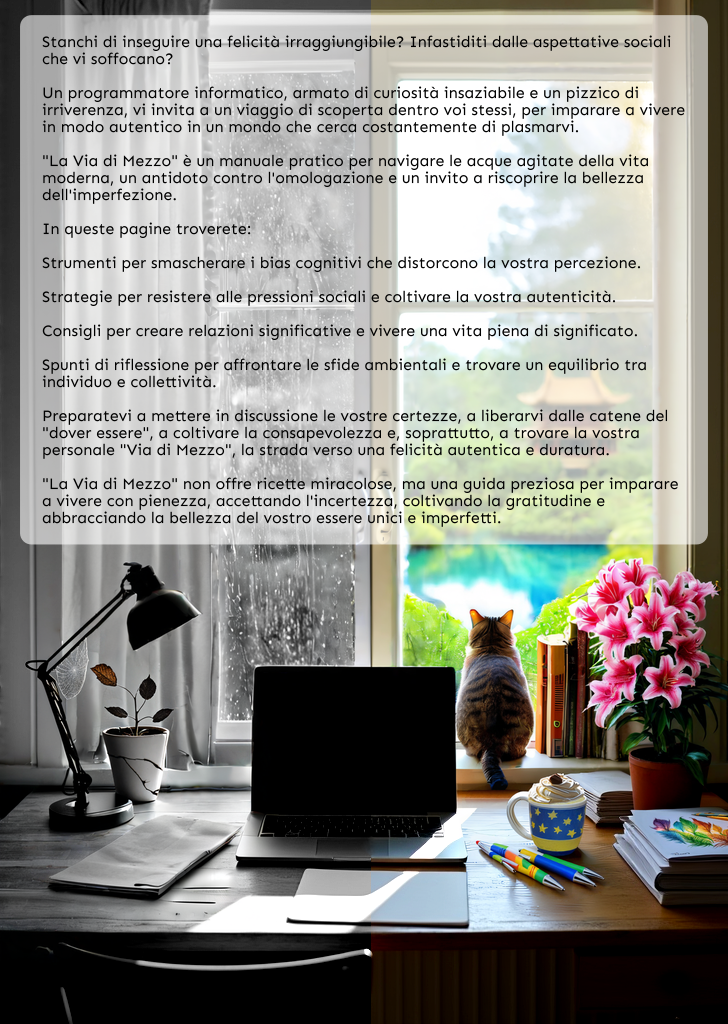
\includegraphics[width=\paperwidth,height=\paperheight]{images/cover_back.png}
    \vspace{-\baselineskip} % Rimuove lo spazio extra sotto l'immagine
\end{figure}

\end{document}